% !TEX root = ../Elements.tex
%%%%%%
% BOOK 10
%%%%%%
\pdfbookmark[0]{Book 10}{book10}
\pagestyle{empty}
\begin{center}
{\Huge ELEMENTS BOOK 10}\\
\spa\spa\spa
{\huge\it Incommensurable Magnitudes\symbolfootnote[2]{The theory of incommensurable magntidues set out in this
book is generally attributed to Theaetetus of Athens. In the footnotes
throughout this book, $k$, $k'$, {\rm etc.}\ stand for distinct ratios
of positive integers.}}
\end{center}
\vspace{3cm}
% Removed epsf size command
\centerline{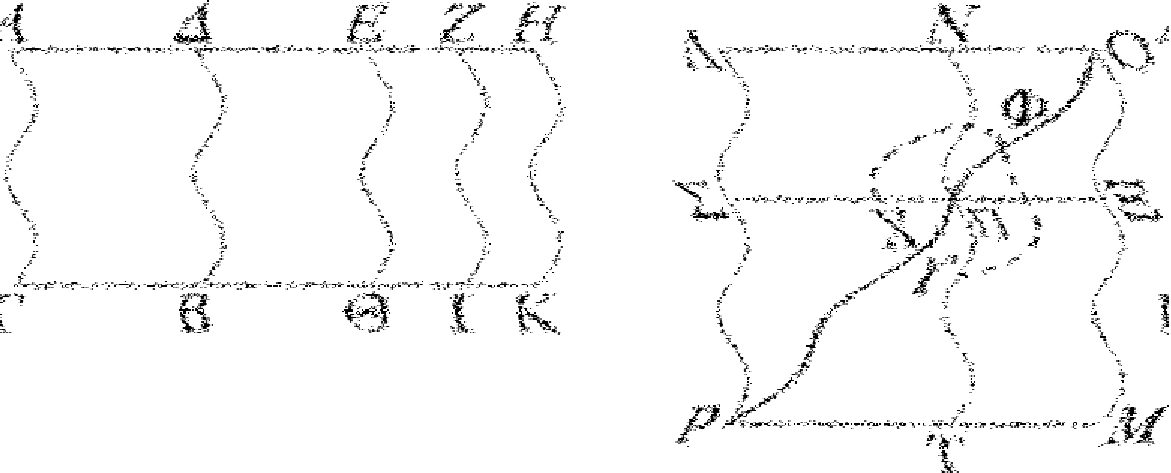
\includegraphics{Book10/front.pdf}}
\newpage

%%%%%%%
% Definitions
%%%%%%%
\pdfbookmark[1]{Definitions I}{def10.1}
\pagestyle{fancy}
\cfoot{\gr{\kern -.7pt }}
\lhead{\large\gr{ΣΤΟΙΘΕΙΩΝ \kern -.7pt {10}.}}
\rhead{\large ELEMENTS BOOK 10}
\begin{Parallel}{}{} 
\ParallelLText{
\begin{center}
\large{\gr{<'Οροι}.}
\end{center}\vspace*{-7pt}

\ggn{1}.~\gr{Σύμμετρα μεγέθη λέγεται τὰ τῶ| α\kern -.7pt  ὐτῶ| μετρῳ
μετρούμενα, ἀσύμμετρα δέ, <ῶν μ\kern -.7pt  ηδὲν ἐνδέθεται κοινὸν
μέτρον γενέσθαι.}

\ggn{2}.~\gr{Εὐθεῖαι δυνάμει σύμμετροί εἰσιν, <όταν τὰ ἀπ>
α\kern -.7pt  ὐτῶν τετράγωνα τῶ| α\kern -.7pt  ὐτῶ| θωρίῳ μετρῆται, ἀσύμμετροι
δέ, <όταν τοῖξ ἀπ> α\kern -.5pt  ὐτῶν τετραγώνοιξ μ\kern -.3pt  ηδὲν ἐνδέθηται θωρίον
κοινὸν μέτρον γενέσθαι.}

\ggn{3}.~\gr{Τούτων ὑποκειμένων δείκνυται, <ότι τῆ| προτεθείσῃ
εὐθείᾳ ὑπάρθουσιν εὐθεῖαι πλήθει >άπειροι σύμμετροί
τε καὶ ἀσύμμετροι αἱ μὲν μ\kern -.7pt  ήκει μόνον, αἱ δὲ καὶ δυνάμει.
καλείσθω ο>ῦν ἡ μὲν προτεθεῖσα εὐθεῖα <ρητή, καὶ
αἱ ταύτῃ σύμμετροι ε>ίτε μ\kern -.7pt  ήκει καὶ δυνάμει ε>ίτε
δυνάμει μόνον <ρηταί, αἱ δὲ ταύτῃ ἀσύμμετροι >άλογοι καλείσθωσαν.}

\ggn{4}.~\gr{Καὶ τὸ μὲν ἀπὸ τῆξ προτεθείσηξ εὐθείαξ τετράγω\-νον <ρητόν,
καὶ τὰ τούτῳ σύμμετρα <ρητά, τὰ δὲ τούτῳ ἀσύμμετρα >άλογα
καλείσθω, καὶ αἱ δυνάμεναι α\kern -.7pt  ὐτὰ >άλογοι, εἰ μὲν τετράγωνα
ε>ίη, α\kern -.7pt  ὐταὶ αἱ πλευραί, εἰ δὲ <έτερά τινα εὐθύγραμμα, αἱ
>ίσα α\kern -.5pt  ὐτοῖξ τετράγωνα ἀναγράφουσαι.}}

\ParallelRText{
\begin{center}
{\large Definitions}
\end{center}

1.~Those magnitudes   measured by the
same measure are said (to be) commensurable, but (those)
of which no (magnitude) admits to be  a common measure (are said to be)
incommensurable.$^\dag$

2.~(Two) straight-lines are commensurable in square$^\ddag$ when the squares on
them are measured by the same area, but (are) incommensurable (in square)
when no area admits to be a common measure of the squares on them.$^\S$

3.~These things being assumed, it is proved that there
exist an infinite multitude of straight-lines commensurable and
incommensurable with an assigned straight-line---those  (incommensurable) in length only, and
those also (commensurable or incommensurable) in square.$^\P$ 
Therefore, let
the assigned straight-line be called rational. And (let) the (straight-lines) commensurable
with it, either in length and square, or in square only, (also be called) rational. But let the (straight-lines) incommensurable with it be called
irrational.$^\ast$ 

4.~And let the square on the assigned straight-line be called  rational. And (let areas) commensurable with it (also be called) rational. But  (let areas) incommensurable with it (be called) irrational, and (let) their square-roots$^\$$ (also be called) irrational---the sides themselves, if the (areas)
are squares, and the (straight-lines) describing squares equal to them, if the (areas) are some other rectilinear (figure).$^\flat$}
\end{Parallel}

{\footnotesize\noindent $^\dag$ In other words, two magnitudes $\alpha$ and
$\beta$ are commensurable if $\alpha:\beta::1:k$, and incommensurable otherwise.\\[0.5ex]
$^\ddag$ Literally, ``in power''.\\[0.5ex]
$^\S$  In other words, two straight-lines of length $\alpha$ and $\beta$ are commensurable in square if $\alpha : \beta::1:k^{1/2}$,  and incommensurable in square otherwise. Likewise, the straight-lines
are commensurable in length if $\alpha:\beta::1:k$, and incommensurable in length otherwise.\\[0.5ex]
$^\P$ To be more exact, straight-lines can either be commensurable in square only, incommensurable in length only, or commenusrable/incommensurable in both
length and square, with an assigned straight-line.\\[0.5ex]
$^\ast$ Let the length of the assigned straight-line be unity. Then rational
straight-lines have lengths expressible as $k$ or $k^{1/2}$, depending on whether the lengths are commensurable in length, or in square only, respectively,
with unity.  All other straight-lines are irrational.\\[0.5ex]
$^\$$ The square-root of an area is the length of the side of an equal area square.\\[0.5ex]
$^\flat$ The area of the  square 
on the assigned straight-line is unity. Rational areas are expressible as $k$.  All other areas are irrational. Thus, squares whose
sides are of rational length have  rational areas, and {\rm vice versa}.}

%%%%%%
% Prop 10.1
%%%%%%
\pdfbookmark[1]{Proposition 10.1}{pdf10.1}
\begin{Parallel}{}{} 
\ParallelLText{
\begin{center}
{\large \ggn{1}.}
\end{center}\vspace*{-7pt}

\gr{Δύο μεγεθῶν ἀνίσων ἐκκειμένων, ἒαν ἀπὸ τοῦ μείζονοξ ἀφαιρεθῆ| μεῖζον >ὴ τὸ <ήμισυ καὶ τοῦ καταλειπομένου μεῖζον >ὴ
τὸ <ήμισυ, καὶ τοῦτο ἀεὶ γίγνηται, λειφθήσεταί τι μέγεθοξ, <ὸ >έσται
>έλασσον τοῦ ἐκκειμένου ἐλάσσονοξ μεγέθουξ.}

\gr{>'Εστω δύο μεγέθη >άνισα τὰ ΑΒ, Γ, <ῶν μεῖζον τὸ ΑΒ; λέγω, <ότι,
ἐαν ἀπὸ τοῦ ΑΒ ἀφαιρεθῆ| μεῖζον >ὴ τὸ <ήμισυ
καὶ τοῦ καταλειπομένου μεῖζον >ὴ τὸ <ήμισυ, καὶ τοῦτο ἀεὶ
γίγνηται, λειφθήσεταί τι μέγεθοξ, <ὸ >έσται >έλασσον τοῦ Γ μεγέθουξ.}\\~\\~\\~\\

% Removed epsf size command
\centerline{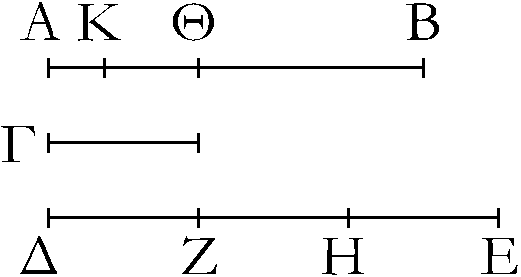
\includegraphics{Book10/fig001g.pdf}}

\gr{Τὸ Γ γὰρ πολλαπλασιαζόμενον >έσται ποτὲ τοῦ ΑΒ μεῖζον. πεπολλαπλασιάσθω, καὶ >έστω τὸ ΔΕ τοῦ μὲν Γ πολλαπλάσιον, τοῦ δὲ ΑΒ
μεῖζον, καὶ διῃρήσθω τὸ ΔΕ εἰξ τὰ τῶ| Γ >ίσα τὰ ΔΖ, ΖΗ, ΗΕ,
καὶ ἀφῃρήσθω ἀπὸ μὲν τοῦ ΑΒ μεῖζον >ὴ τὸ <ήμισυ τὸ ΒΘ,
ἀπὸ δὲ τοῦ ΑΘ μεῖζον >ὴ τὸ <ήμισυ τὸ ΘΚ, καὶ τοῦτο
ἀεὶ γιγνέσθω, <έωξ >ὰν αἱ ἐν τῶ| ΑΒ διαιρέσειξ ἰσοπληθεῖξ
γένωνται ταῖξ ἐν τῶ| ΔΕ διαιρέσεσιν.}

\gr{>'Εστωσαν ο>ῦν αἱ ΑΚ, ΚΘ, ΘΒ διαιρέσειξ ἰσοπληθεῖξ ο>ῦσαι ταῖξ
ΔΖ, ΖΗ, ΗΕ; καὶ ἐπεὶ μεῖζόν ἐστι τὸ ΔΕ τοῦ ΑΒ, καὶ ἀφή|ρηται
ἀπὸ μὲν τοῦ ΔΕ >έλασσον τοῦ ἡμίσεωξ τὸ ΕΗ, ἀπὸ δὲ τοῦ ΑΒ
μεῖζον >ὴ τὸ <ήμισυ τὸ ΒΘ, λοιπὸν >άρα τὸ ΗΔ λοιποῦ τοῦ ΘΑ
μεῖζόν ἐστιν. καὶ ἐπεὶ μεῖζόν ἐστι τὸ ΗΔ τοῦ ΘΑ, καὶ
ἀφή|ρηται τοῦ μὲν ΗΔ <ήμισυ τὸ ΗΖ, τοῦ δὲ ΘΑ μεῖζον >ὴ
τὸ <ήμισυ τὸ ΘΚ, λοιπὸν >άρα τὸ ΔΖ λοιποῦ τοῦ ΑΚ μεῖζόν ἐστιν.
>ίσον δὲ τὸ ΔΖ τῶ| Γ; καὶ τὸ Γ >άρα τοῦ ΑΚ μεῖζόν ἐστιν.
>έλασσον >άρα τὸ ΑΚ τοῦ Γ.}

\gr{Καταλείπεται >άρα ἀπὸ τοῦ ΑΒ μεγέθουξ τὸ ΑΚ μέγεθοξ >έλασσον >ὸν
τοῦ ἐκκειμένου ἐλάσσονοξ μεγέθουξ τοῦ Γ; <όπερ >έδει δεῖχαι.}\,---\,\gr{ὁμοίωξ δὲ δειθθήσεται, κ>ὰν ἡμίση >ῆ| τὰ ἀφαιρούμενα.}}

\ParallelRText{
\begin{center}
{\large Proposition 1}$^\dag$
\end{center}

If, from
the greater of two unequal magnitudes (which are) laid out,  (a part) greater than half is subtracted, and (if from) the remainder (a part) greater than
half (is subtracted), and (if) this happens continually, then some magnitude will (eventually) be left which
will be less than the  lesser laid out magnitude.

Let $AB$ and $C$ be two unequal magnitudes, of which (let) $AB$ (be) the greater. I say that if (a part) greater than half is subtracted  from $AB$,
and (if a part) greater than half (is subtracted) from the remainder, and (if) this happens
continually, then some magnitude will (eventually) be left which will be less
than the magnitude $C$. 

% Removed epsf size command
\centerline{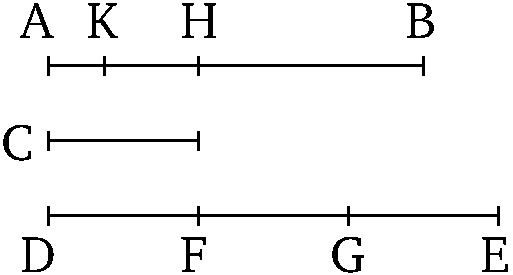
\includegraphics{Book10/fig001e.pdf}}

For $C$, when multiplied (by some number), will sometimes be greater than $AB$ [Def.~5.4]. Let it 
 be (so) multiplied. And let $DE$ be (both) a multiple of $C$, and greater
than $AB$. And let $DE$ be divided into the (divisions) $DF$, $FG$,
$GE$, equal to $C$. And   let $BH$, (which is) greater than half, be subtracted from $AB$. And  (let) $HK$, (which is) greater than half, (be subtracted) from $AH$. And let this happen continually, until the divisions in
$AB$ become equal in number to the divisions in $DE$.

Therefore, let the divisions (in $AB$) be $AK$, $KH$, $HB$, being equal in number to $DF$, $FG$, $GE$.  And since $DE$ is greater than $AB$, and $EG$, (which is) less than half, has been subtracted from $DE$, and $BH$, (which is) greater
than half, from $AB$, the remainder $GD$ is thus greater than the remainder
$HA$. And since $GD$ is greater than $HA$, and the half $GF$ has been
subtracted from $GD$, and $HK$, (which is) greater than half, from $HA$,
the remainder $DF$ is thus greater than the remainder $AK$. And $DF$
(is) equal to $C$. $C$ is thus also greater than $AK$.
Thus, $AK$ (is) less than $C$.

Thus, the magnitude $AK$,  which is less
than the lesser laid out magnitude $C$, is left over from the magnitude $AB$. (Which is) the very thing it was required to show. --- (The theorem) can similarly be proved even if  the
(parts) subtracted are halves.}
\end{Parallel}
{\footnotesize\noindent $^\dag$ This theorem is the basis of the so-called {\rm method of exhaustion}, and is generally attributed to Eudoxus of Cnidus.}

%%%%%%
% Prop 10.2
%%%%%%
\pdfbookmark[1]{Proposition 10.2}{pdf10.2}
\begin{Parallel}{}{} 
\ParallelLText{
\begin{center}
{\large \ggn{2}.}
\end{center}\vspace*{-7pt}

\gr{Ἐὰν δύο μεγεθῶν [ἐκκειμένων] ἀνίσων ἀνθυφαιρουμένου ἀεὶ
τοῦ ἐλάσσονοξ ἀπὸ τοῦ μείζονοξ τὸ καταλειπόμενον μ\kern -.7pt  ηδέποτε
καταμετρῆ| τὸ πρὸ ἑαυτοῦ, ἀσύμμετρα >έσται τὰ μεγέθη.}\\

% Removed epsf size command
\centerline{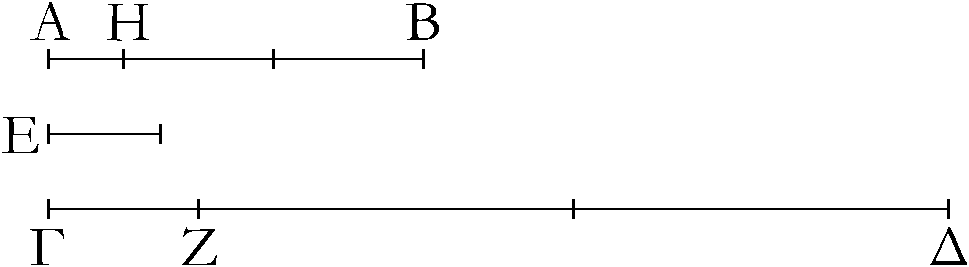
\includegraphics{Book10/fig002g.pdf}}

\gr{Δύο γὰρ μεγεθῶν >όντων ἀνίσων τῶν ΑΒ, ΓΔ καὶ ἐλάσσονοξ
τοῦ ΑΒ ἀνθυφαιρουμένου ἀεὶ τοῦ ἐλάσσονοξ ἀπὸ τοῦ μείζονοξ τὸ
περιλειπόμενον μ\kern -.7pt  ηδέποτε καταμετρείτω τὸ πρὸ ἑαυτοῦ; λέγω, <ότι
ἀσύμμετρά ἐστι τὰ ΑΒ, ΓΔ μεγέθη.}

\gr{Εἰ γάρ ἐστι σύμμετρα, μετρήσει τι α\kern -.7pt  ὐτὰ μέγεθοξ. μετρείτω, εἰ δυνατόν,
καὶ >έστω τὸ Ε; καὶ τὸ μὲν ΑΒ τὸ ΖΔ καταμετροῦν λειπέτω ἑαυτοῦ
>έλασσον τὸ ΓΖ, τὸ δὲ ΓΖ τὸ ΒΗ καταμετροῦν λειπέτω ἑαυτοῦ
>έλασσον τὸ ΑΗ, καὶ τοῦτο ἀεὶ γινέσθω, <έωξ ο<ῦ λειφθῆ| τι
μέγεθοξ, <ό ἐστιν >έλασσον τοῦ Ε. γεγονέτω, καὶ λελείφθω τὸ ΑΗ
>έλασσον τοῦ Ε. ἐπεὶ ο>ῦν τὸ Ε τὸ ΑΒ μετρεῖ, ἀλλὰ τὸ ΑΒ τὸ
ΔΖ μετρεῖ, καὶ τὸ Ε >άρα τὸ ΖΔ μετρήσει. μετρεῖ δὲ καὶ <όλον
τὸ ΓΔ; καὶ λοιπὸν >άρα τὸ ΓΖ μετρήσει. ἀλλὰ τὸ ΓΖ τὸ ΒΗ μετρεῖ;
καὶ τὸ Ε >άρα τὸ ΒΗ μετρεῖ. μετρεῖ δὲ καὶ <όλον τὸ ΑΒ; καὶ λοιπὸν
>άρα τὸ ΑΗ μετρήσει, τὸ μεῖζον τὸ >έλασσον; <όπερ ἐστὶν ἀδύνατον.
οὐκ >άρα τὰ ΑΒ, ΓΔ μεγέθη μετρήσει τι μέγεθοξ; ἀσύμμετρα >άρα
ἐστὶ τὰ ΑΒ, ΓΔ μεγέθη.}

\gr{Ἐὰν >άρα δύο μεγεθῶν ἀνίσων, καὶ τὰ ἑχῆξ.}}

\ParallelRText{
\begin{center}
{\large Proposition 2}
\end{center}

If the remainder of two unequal magnitudes (which are) [laid out] never measures the (magnitude) before it, (when) the lesser (magnitude is) continually subtracted in turn from the greater, then the (original) magnitudes will be incommensurable.

% Removed epsf size command
\centerline{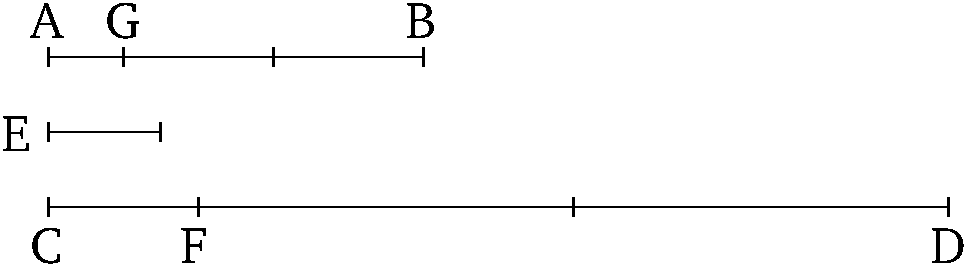
\includegraphics{Book10/fig002e.pdf}}

For, $AB$ and $CD$ being two unequal magnitudes, and $AB$ (being) the lesser, let the remainder
never measure the (magnitude) before it,
(when) the lesser (magnitude is) continually subtracted in turn from the greater. I say that
the magnitudes $AB$ and $CD$ are incommensurable.

For if they are commensurable then some magnitude will measure them (both). If possible, let it
(so) measure (them),  and let it be $E$. And let $AB$ leave $CF$
less than itself (in) measuring $FD$, and let $CF$ leave $AG$ less than
itself (in) measuring $BG$, and let this happen continually, until  some magnitude which is less than  $E$ is left. Let (this) have occurred,$^\dag$ and
let $AG$, (which is) less than $E$, be left. Therefore, since
$E$ measures $AB$, but $AB$ measures $DF$, $E$ will thus also measure $FD$. And it also measures the whole (of) $CD$. Thus, it will
also measure the remainder  $CF$. But, $CF$ measures $BG$. Thus,
$E$ also measures $BG$. And it also measures the whole (of) $AB$. 
Thus, it will also measure the remainder $AG$, the greater (measuring)
the lesser. The very thing is impossible. Thus, some magnitude cannot
measure (both) the magnitudes $AB$ and $CD$. Thus, the
magnitudes $AB$ and $CD$ are incommensurable [Def.~10.1].

Thus, if \ldots of two unequal magnitudes, and so on \ldots.}
\end{Parallel}
{\footnotesize\noindent$^\dag$ The fact that this will eventually occur is guaranteed by
Prop.~10.1.}

%%%%%%
% Prop 10.3
%%%%%%
\pdfbookmark[1]{Proposition 10.3}{pdf10.3}
\begin{Parallel}{}{} 
\ParallelLText{
\begin{center}
{\large \ggn{3}.}
\end{center}\vspace*{-7pt}

\gr{Δύο μεγεθῶν συμμέτρων δοθέντων τὸ μέγιστον α\kern -.7pt  ὐτῶν κοινὸν
μέτρον εὑρεῖν.}

% Removed epsf size command
\centerline{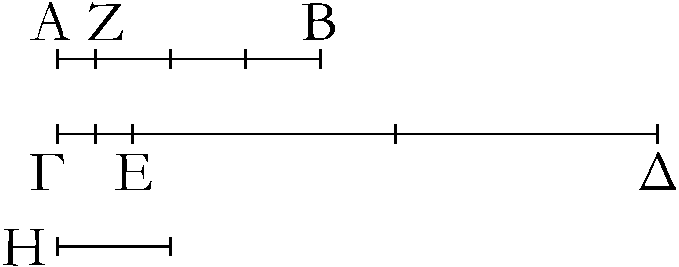
\includegraphics{Book10/fig003g.pdf}}

\gr{>'Εστω τὰ δοθέντα δύο μεγέθη σύμμετρα τὰ ΑΒ, ΓΔ, <ῶν
>έλασσον τὸ ΑΒ; δεῖ δὴ τῶν ΑΒ, ΓΔ τὸ μέγιστον κοινὸν μέτρον
εὑρεῖν.}

\gr{Τὸ ΑΒ γὰρ μέγεθοξ >ήτοι μετρεῖ τὸ ΓΔ >ὴ ο>ύ. εἰ
μὲν ο>ῦν μετρεῖ, μετρεῖ δὲ καὶ ἑαυτό, τὸ ΑΒ >άρα τῶν
ΑΒ, ΓΔ κοινὸν μέτρον ἐστίν; καὶ φανερόν, <ότι καὶ
μέγιστον. μεῖζον γὰρ τοῦ ΑΒ μεγέθουξ τὸ ΑΒ οὐ
μετρήσει.}

\gr{μ\kern -.7pt  ὴ μετρείτω δὴ τὸ ΑΒ τὸ ΓΔ. καὶ ἀνθυφαιρουμένου ἀεὶ τοῦ ἐλάσσονοξ ἀπὸ τοῦ  μείζονοξ, τὸ περιλειπόμενον μετρήσει
ποτὲ τὸ πρὸ ἑαυτοῦ διὰ τὸ μ\kern -.7pt  ὴ ε>ῖναι ἀσύμμετρα τὰ
ΑΒ, ΓΔ; καὶ τὸ μὲν ΑΒ τὸ ΕΔ καταμετροῦν λειπέτω ἑαυτοῦ
>έλασσον τὸ ΕΓ, τὸ δὲ ΕΓ τὸ ΖΒ καταμετροῦν λειπέτω ἑαυτοῦ
>έλασσον τὸ ΑΖ, τὸ δὲ ΑΖ τὸ ΓΕ μετρείτω.}

\gr{Ἐπεὶ ο>ῦν τὸ ΑΖ τὸ ΓΕ μετρεῖ, ἀλλὰ τὸ ΓΕ τὸ ΖΒ μετρεῖ, καὶ
τὸ ΑΖ >άρα τὸ ΖΒ μετρήσει. μετρεῖ δὲ καὶ ἑαυτό; καὶ <όλον >άρα
τὸ ΑΒ μετρήσει τὸ ΑΖ. ἀλλὰ τὸ ΑΒ τὸ ΔΕ μετρεῖ; καὶ τὸ ΑΖ >άρα
τὸ ΕΔ μετρήσει. μετρεῖ δὲ καὶ τὸ ΓΕ; καί <όλον >άρα τὸ ΓΔ
μετρεῖ; τὸ ΑΖ >άρα τῶν ΑΒ, ΓΔ κοινὸν μέτρον ἐστίν. λέγω δή,
<ότι καὶ μέγιστον. εἰ γὰρ μ\kern -.7pt  ή, >έσται τι μέγεθοξ μεῖζον τοῦ ΑΖ,
<ὸ
μετρήσει τὰ ΑΒ, ΓΔ. >έστω τὸ Η. ἐπεὶ ο>ῦν τὸ Η τὸ ΑΒ
μετρεῖ, ἀλλὰ τὸ ΑΒ τὸ ΕΔ μετρεῖ, καὶ τὸ Η >άρα τὸ ΕΔ μετρήσει. μετρεῖ δὲ καὶ <όλον τὸ ΓΔ; καὶ λοιπὸν >άρα τὸ ΓΕ μετρήσει
τὸ Η. ἀλλὰ τὸ ΓΕ τὸ ΖΒ μετρεῖ; καὶ τὸ Η >άρα
τὸ ΖΒ μετρήσει. μετρεῖ δὲ καὶ <όλον τὸ ΑΒ, καὶ λοιπὸν τὸ ΑΖ
μετρήσει, τὸ μεῖζον τὸ >έλασσον; <όπερ ἐστὶν ἀδύνατον. οὐκ
>άρα μεῖζόν τι μέγεθοξ τοῦ ΑΖ τὰ ΑΒ, ΓΔ μετρήσει; τὸ ΑΖ >άρα
τῶν ΑΒ, ΓΔ τὸ μέγιστον κοινὸν μέτρον ἐστίν.}

\gr{Δύο >άρα μεγεθῶν συμμέτρων δοθέντων τῶν ΑΒ, ΓΔ τὸ μέγιστον
κοινὸν μέτρον η<ύρηται; <όπερ
>έδει δεῖχαι.}\\~\\~\\~\\~\\~\\~\\

\begin{center}
{\large \gr{Πόρισμα}.}
\end{center}\vspace*{-7pt}

\gr{Ἐκ δὴ τούτου φανερόν, <ότι, ἒαν μέγεθοξ δύο μεγέθη μετρῆ|, καὶ
τὸ μέγιστον α\kern -.7pt  ὐτῶν κοινὸν μέτρον μετρήσει.}}

\ParallelRText{
\begin{center}
{\large Proposition 3}
\end{center}

To find the greatest common measure of two
given commensurable magnitudes.

% Removed epsf size command
\centerline{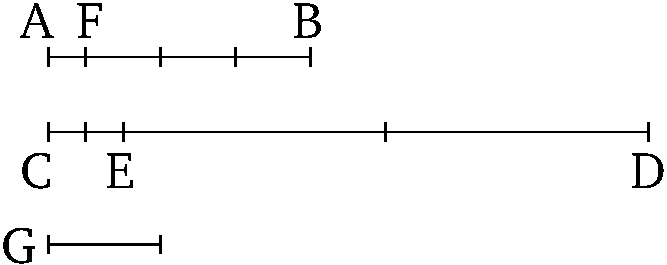
\includegraphics{Book10/fig003e.pdf}}

Let $AB$ and $CD$ be the two given magnitudes, of which (let) $AB$ (be)
the lesser. So, it is required to find the greatest common measure of
$AB$ and $CD$.

For the magnitude $AB$ either measures, or (does) not (measure), $CD$. Therefore, if
it measures ($CD$), and (since) it also measures itself, $AB$ is thus
a common measure of $AB$ and $CD$. And (it is) clear that (it is) also
(the) greatest. For a (magnitude) greater than magnitude $AB$ cannot
measure $AB$.

So let $AB$ not measure $CD$. And continually subtracting in turn the lesser 
(magnitude) from the greater, the remaining (magnitude) will (at) some time measure the (magnitude)
before it, on account of $AB$ and $CD$ not being incommensurable [Prop.~10.2]. And let $AB$ leave $EC$ less than
itself (in) measuring $ED$, and let $EC$ leave $AF$ less than itself (in)
measuring $FB$, and let $AF$ measure $CE$.

Therefore, since $AF$ measures $CE$, but $CE$ measures $FB$, $AF$
will thus also measure $FB$. And it also measures itself. Thus, $AF$
will also measure the whole (of) $AB$. But, $AB$ measures $DE$. Thus, $AF$
will also measure $ED$. And it also measures $CE$. Thus, it also measures the whole of $CD$. Thus, $AF$ is a common measure of $AB$ and $CD$.
So I say that (it is) also (the) greatest (common measure). For, if not,
there will be some magnitude, greater than $AF$, which will measure
(both) $AB$ and $CD$. Let it be $G$. Therefore, since $G$ measures $AB$,
but $AB$ measures $ED$, $G$ will thus also measure $ED$. And
it also measures the whole of $CD$. Thus, $G$ will also measure the remainder $CE$.
But $CE$ measures $FB$. Thus, $G$ will also measure $FB$. And
it also measures the whole (of) $AB$. And (so) it will measure the
remainder $AF$, the greater (measuring) the lesser. The very thing is impossible. Thus, some magnitude greater than $AF$ cannot measure
(both) $AB$ and $CD$. Thus, $AF$ is the greatest common measure of
$AB$ and $CD$.

Thus, the greatest common measure of two given commensurable magnitudes, $AB$ and $CD$, has been found. (Which is) the very thing
it was required to show.\\

\begin{center}
{\large Corollary}
\end{center}\vspace*{-7pt}

So (it is) clear, from this, that if a magnitude measures two magnitudes
then it will also measure their greatest common measure.}
\end{Parallel}

%%%%%%
% Prop 10.4
%%%%%%
\pdfbookmark[1]{Proposition 10.4}{pdf10.4}
\begin{Parallel}{}{} 
\ParallelLText{
\begin{center}
{\large \ggn{4}.}
\end{center}\vspace*{-7pt}

\gr{Τριῶν μεγεθῶν συμμέτρων δοθέντων τὸ μέγιστον α\kern -.7pt  ὐτῶν
κοινὸν μέτρον εὑρεῖν.}

% Removed epsf size command
\centerline{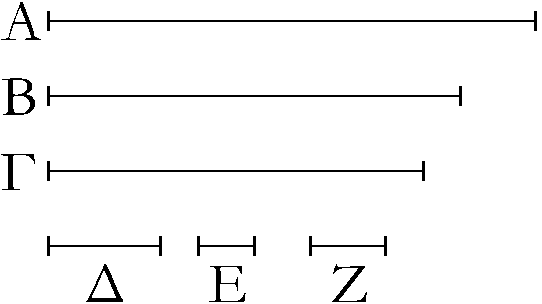
\includegraphics{Book10/fig004g.pdf}}

\gr{>'Εστω τὰ δοθέντα τρία μεγέθη σύμμετρα τὰ Α, Β, Γ; δεῖ δὴ τῶν
Α, Β, Γ τὸ μέγιστον κοινὸν μέτρον εὑρεῖν.}

\gr{Εἰλήφθω γὰρ δύο τῶν Α, Β τὸ μέγιστον κοινὸν μέτρον, καὶ >έστω
τὸ Δ; τὸ δὴ Δ τὸ Γ >ήτοι μετρεῖ >ὴ ο>ύ [μετρεῖ]. μετρείτω πρότερον.
ἐπεὶ ο>ῦν τὸ Δ τὸ Γ μετρεῖ, μετρεῖ δὲ καὶ τὰ Α, Β, τὸ Δ >άρα
τὰ Α, Β, Γ μετρεῖ; τὸ Δ >άρα τῶν Α, Β, Γ κοινὸν μέτρον ἐστίν.
καὶ φανερόν, <ότι καὶ μέγιστον; μεῖζον γὰρ τοῦ Δ μεγέθουξ τὰ Α, Β
οὐ μετρεῖ.}

\gr{μ\kern -.7pt  ὴ μετρείτω δὴ τὸ Δ τὸ Γ. λέγω πρῶτον, <ότι
σύμμετρά ἐστι τὰ Γ, Δ. ἐπεὶ γὰρ σύμμετρά ἐστι τὰ Α, Β, Γ, μετρήσει τι 
α\kern -.7pt  ὐτὰ μέγεθοξ, <ὸ δηλαδὴ καὶ τὰ Α, Β μετρήσει; <ώστε καὶ τὸ τῶν
Α, Β μέγιστον κοινὸν μέτρον τὸ Δ μετρήσει. μετρεῖ δὲ καὶ τὸ Γ;
<ώστε τὸ εἰρημένον μέγεθοξ μετρήσει τὰ Γ, Δ; σύμμετρα >άρα 
ἐστὶ τὰ Γ, Δ. εἰλήφθω ο>ῦν α\kern -.5pt  ὐτῶν τὸ μέγιστον κοινὸν μέτρον,
καὶ >έστω τὸ Ε. ἐπεὶ ο>ῦν τὸ Ε τὸ Δ μετρεῖ, ἀλλὰ τὸ Δ τὰ Α, Β
μετρεῖ, καὶ τὸ Ε >άρα τὰ Α, Β μετρήσει. μετρεῖ δὲ καὶ τὸ Γ.
τὸ Ε >άρα τὰ Α, Β, Γ μετρεῖ; τὸ Ε >άρα τῶν Α, Β, Γ κοινόν ἐστι
μέτρον. λέγω δή, <ότι καὶ μέγιστον. εἰ γὰρ δυνατόν, >έστω τι τοῦ
Ε μεῖζον μέγεθοξ τὸ Ζ, καὶ μετρείτω τὰ Α, Β, Γ. καὶ ἐπεὶ τὸ
Ζ τὰ Α, Β, Γ μετρεῖ, καὶ τὰ Α, Β >άρα μετρήσει καὶ τὸ τῶν Α, Β
μέγιστον κοινὸν μέτρον μετρήσει. τὸ δὲ τῶν Α, Β μέγιστον κοινὸν
μέτρον ἐστὶ τὸ Δ; τὸ Ζ >άρα τὸ Δ μετρεῖ. μετρεῖ δὲ καὶ τὸ Γ; τὸ Ζ
>άρα τὰ Γ, Δ μετρεῖ; καὶ τὸ τῶν Γ, Δ >άρα μέγιστον κοινὸν
μέτρον μετρήσει τὸ Ζ. >έστι δὲ τὸ Ε; τὸ Ζ >άρα τὸ Ε μετρήσει,
τὸ μεῖζον τὸ >έλασσον; <όπερ ἐστὶν ἀδύνατον. οὐκ >άρα μεῖζόν
τι τοῦ Ε μεγέθουξ [μέγεθοξ] τὰ Α, Β, Γ μετρεῖ; τὸ Ε >άρα τῶν Α, Β, Γ τὸ μέγιστον κοινὸν μέτρον ἐστίν, ἒαν μ\kern -.3pt  ὴ μετρῆ| τὸ Δ τὸ Γ, ἒαν
δὲ μετρῆ|, α\kern -.7pt  ὐτὸ τὸ Δ.}

\gr{Τριῶν >άρα μεγεθῶν συμμέτρων δοθέντων τὸ μέγιστον κοινὸν
μέτρον η<ύρηται [<όπερ >έδει δεῖχαι].}\\~\\~\\~\\~\\~\\~\\~\\~\\~\\

\begin{center}
{\large \gr{Πόρισμα}.}
\end{center}\vspace*{-7pt}

\gr{Ἐκ δὴ τούτου φανερόν, <ότι, ἒαν μέγεθοξ τρία μεγέθη μετρῆ|, καὶ
τὸ μέγιστον α\kern -.7pt  ὐτῶν κοινὸν μέτρον μετρήσει.}

\gr{Ὁμοίωξ δὴ καὶ ἐπὶ πλειόνων τὸ μέγιστον κοινὸν
μέτρον ληφθήσεται, καὶ τὸ πόρισμα προθωρήσει. <όπερ >έδει δεῖχαι.}}

\ParallelRText{
\begin{center}
{\large Proposition 4}
\end{center}

To find the greatest common measure of three
given commensurable magnitudes.

% Removed epsf size command
\centerline{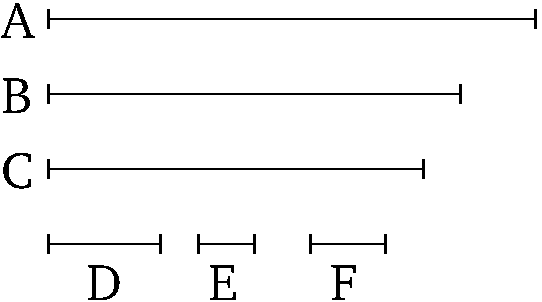
\includegraphics{Book10/fig004e.pdf}}

Let $A$, $B$, $C$ be the three given commensurable magnitudes. So
it is required to find the greatest common measure of $A$, $B$, $C$.

For let the greatest common measure of the two (magnitudes)
$A$ and $B$ be taken [Prop.~10.3],
and let it be $D$. So $D$ either measures, or [does] not
[measure], $C$. Let it, first of all, measure ($C$). Therefore, since
$D$ measures $C$, and it also measures $A$ and $B$, $D$ thus
measures $A$, $B$, $C$. Thus, $D$ is a common measure of $A$, $B$, $C$.
And (it is) clear that (it is) also (the) greatest (common measure). For
no magnitude larger than $D$ measures (both) $A$ and $B$.

So let $D$ not measure $C$. I say, first, that $C$ and $D$ are
commensurable. For if $A$, $B$, $C$ are commensurable then some
magnitude will measure them which will clearly also measure $A$ and $B$.
Hence, it will also measure $D$, the greatest common measure of $A$ and $B$ [Prop.~10.3~corr.]. And it also measures
$C$. Hence, the aforementioned magnitude will measure (both)
$C$ and $D$. Thus, $C$ and $D$ are commensurable [Def.~10.1]. Therefore, let their
greatest common measure be taken [Prop.~10.3], and let it be $E$. Therefore, since
$E$ measures $D$, but $D$ measures (both) $A$ and $B$, $E$ will
thus also measure $A$ and $B$. And it also measures $C$. Thus,
$E$ measures $A$, $B$, $C$. Thus, $E$ is a common measure of $A$, $B$, $C$.  So I say that (it is) also (the) greatest (common measure). For, if
possible, let $F$ be some magnitude greater than $E$, and let it
measure $A$, $B$, $C$. And since $F$ measures $A$, $B$, $C$, it will
thus also measure $A$ and $B$, and  will (thus) measure the greatest common measure of $A$ and $B$ [Prop.~10.3~corr.].  And
$D$ is the greatest common measure of $A$ and $B$.  Thus, $F$ measures $D$. And it also measures $C$. Thus, $F$ measures (both) $C$ and $D$.
Thus, $F$ will also measure the greatest common measure of $C$ and $D$  [Prop.~10.3~corr.].
And it is $E$. Thus, $F$ will measure $E$, the greater (measuring)
the lesser. The very thing is impossible. Thus, some [magnitude]
greater than the magnitude $E$ cannot measure $A$, $B$, $C$. Thus,
if $D$ does not
measure $C$ then
$E$ is the greatest common measure of $A$, $B$, $C$.  And if it does measure ($C$) then $D$ itself (is the
greatest common measure).

Thus, the greatest common measure  of three given
commensurable magnitudes has been found.  [(Which is) the very thing it was required to
show.]\\

\begin{center}
{\large Corollary}
\end{center}\vspace*{-7pt}

So (it is) clear, from this, that if a magnitude measures three
magnitudes then it will also measure their greatest common measure.

So, similarly, the greatest common measure of more (magnitudes) can also be
taken, and the (above) corollary will go forward. (Which is) the very thing
it was required to show.}
\end{Parallel}

%%%%%%
% Prop 10.5
%%%%%%
\pdfbookmark[1]{Proposition 10.5}{pdf10.5}
\begin{Parallel}{}{} 
\ParallelLText{
\begin{center}
{\large \ggn{5}.}
\end{center}\vspace*{-7pt}

\gr{Τὰ σύμμετρα μεγέθη πρὸξ >άλληλα λόγον >έθει, <ὸν ἀριθμὸξ πρὸξ
ἀριθμόν.}

% Removed epsf size command
\centerline{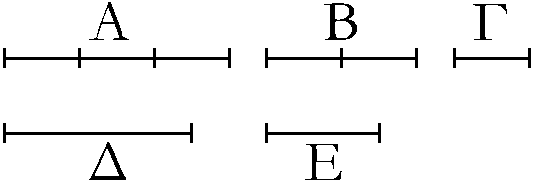
\includegraphics{Book10/fig005g.pdf}}

\gr{>'Εστω σύμμετρα μεγέθη τὰ Α, Β; λέγω, <ότι τὸ Α πρὸξ τὸ Β λόγον >έθει,
<ὸν ἀριθμὸξ πρὸξ ἀριθμόν.}

\gr{Ἐπεὶ γὰρ σύμμετρά ἐστι τὰ Α, Β, μετρήσει τι α\kern -.7pt  ὐτὰ μέγεθοξ. μετρείτω,
καὶ >έστω τὸ Γ. καὶ ὁσάκιξ τὸ Γ τὸ Α μετρεῖ, τοσα\kern -.7pt  ῦται μονάδεξ
>έστωσαν ἐν τῶ| Δ, ὁσάκιξ δὲ τὸ Γ τὸ Β μετρεῖ, τοσα\kern -.5pt  ῦται μονάδεξ
>έστωσαν ἐν τῶ| Ε.}

\gr{Ἐπεὶ ο>ῦν τὸ Γ τὸ Α μετρεῖ κατὰ τὰξ ἐν τῶ| Δ μονάδαξ, 
μετρεῖ δὲ καὶ ἡ μονὰξ τὸν Δ κατὰ τὰξ ἐν α\kern -.7pt  ὐτῶ| μονάδαξ,
ἰσάκιξ
>άρα ἡ μονὰξ τὸν Δ μετρεῖ ἀριθμὸν καὶ τὸ Γ μέγεθοξ τὸ Α; >έστιν
>άρα ὡξ τὸ Γ πρὸξ τὸ Α, ο<ύτωξ ἡ μονὰξ πρὸξ τὸν Δ; ἀνάπαλιν
>άρα, ὡξ τὸ Α πρὸξ τὸ Γ, ο<ύτωξ ὁ Δ πρὸξ τὴν μονάδα. πάλιν
ἐπεὶ τὸ Γ τὸ Β μετρεῖ κατὰ τὰξ ἐν τῶ| Ε μονάδαξ, μετρεῖ
δὲ καὶ ἡ μονὰξ τὸν Ε κατὰ τὰξ ἐν α\kern -.7pt  ὐτῶ| μονάδαξ, ἰσάκιξ
>άρα ἡ μονὰξ τὸν Ε μετρεῖ καὶ τὸ Γ τὸ Β; >έστιν >άρα ὡξ τὸ Γ
πρὸξ τὸ Β, ο<ύτωξ ἡ μονὰξ πρὸξ τὸν Ε. ἐδείθθη δὲ καὶ ὡξ τὸ
Α πρὸξ τὸ Γ, ὁ Δ πρὸξ τὴν μονάδα; δι> >ίσου >άρα ἐστὶν ὡξ τὸ
Α πρὸξ τὸ Β, ο<ύτωξ ὁ Δ ἀριθμὸξ πρὸξ τὸν Ε.}

\gr{Τὰ >άρα σύμμετρα μεγέθη τὰ Α, Β πρὸξ >άλληλα λόγον >έθει,
<ὸν ἀριθμὸξ ὁ Δ πρὸξ ἀριθμὸν τὸν Ε; <όπερ >έδει δεῖχαι.}}

\ParallelRText{
\begin{center}
{\large Proposition 5}
\end{center}

Commensurable magnitudes have to one another the
ratio which (some) number (has) to (some) number.

% Removed epsf size command
\centerline{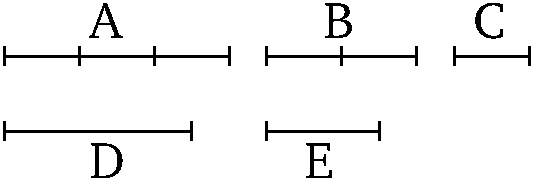
\includegraphics{Book10/fig005e.pdf}}

Let $A$ and $B$ be commensurable magnitudes. I say that $A$ has to $B$
the ratio which (some) number (has) to (some) number.

For if $A$ and $B$ are commensurable (magnitudes) then some magnitude
will measure them. Let it (so) measure (them), and let it be $C$. And
as many times as $C$ measures $A$, so many units let there be in
$D$. And as many times as $C$ measures $B$, so many units let there be
in $E$.

Therefore, since $C$ measures $A$ according to the units in $D$, and
a unit also measures $D$ according to the units in it,  a unit thus measures the
number $D$ as many times as the magnitude $C$ (measures) $A$. 
Thus, as $C$ is to $A$, so a unit (is) to $D$ [Def.~7.20].$^\dag$ Thus, inversely, as $A$ (is) to $C$, so
$D$ (is) to a unit [Prop.~5.7~corr.]. Again, since
$C$ measures $B$ according to the units in $E$, and a unit also measures $E$ according to the units in it,   a unit thus measures $E$ the
same number of times that $C$ (measures) $B$. Thus, as $C$ is to $B$, so
a unit (is) to $E$ [Def.~7.20]. And it was also
shown that as $A$ (is) to $C$, so $D$ (is) to a unit. Thus, via equality,
as $A$ is to $B$, so the number $D$ (is) to the (number) $E$ [Prop.~5.22].

Thus, the commensurable magnitudes $A$ and $B$ have to one another
the ratio which the number $D$ (has) to the number $E$. (Which is) the
very thing it was required to show.}
\end{Parallel}
{\footnotesize\noindent$^\dag$ There is a slight logical gap here, since Def.~7.20  applies to four numbers, rather than two number and two magnitudes.}

%%%%%%
% Prop 10.6
%%%%%%
\pdfbookmark[1]{Proposition 10.6}{pdf10.6}
\begin{Parallel}{}{} 
\ParallelLText{
\begin{center}
{\large \ggn{6}.}
\end{center}\vspace*{-7pt}

\gr{Ἐὰν δύο μεγέθη πρὸξ >άλληλα λόγον >έθῃ, <ὸν ἀριθμὸξ πρὸξ
ἀριθμόν, σύμμετρα >έσται τὰ μεγέθη.}\\

% Removed epsf size command
\centerline{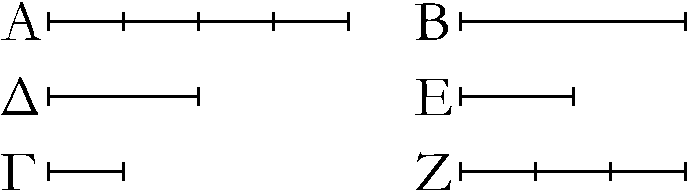
\includegraphics{Book10/fig006g.pdf}}

\gr{Δύο γὰρ μεγέθη τὰ Α, Β πρὸξ >άλληλα λόγον ἐθέτω, <ὸν ἀριθμὸξ
ὁ Δ πρὸξ ἀριθμὸν τὸν Ε; λέγω, <ότι σύμμετρά ἐστι τὰ Α, Β
μεγέθη.}

\gr{<'Οσαι γάρ εἰσιν ἐν τῶ| Δ μονάδεξ, εἰξ τοσα\kern -.7pt  ῦτα >ίσα
διῃρήσθω τὸ Α, καὶ ἑνὶ α\kern -.7pt  ὐτῶν >ίσον >έστω τὸ Γ; <όσαι
δέ εἰσιν ἐν τῶ| Ε μονάδεξ, ἐκ τοσούτων μεγεθῶν >ίσων
τῶ| Γ συγκείσθω τὸ Ζ.}

\gr{Ἐπεὶ ο>ῦν, <όσαι εἰσὶν ἐν τῶ| Δ μονάδεξ, τοσα\kern -.7pt  ῦτά εἰσι
καὶ ἐν τῶ| Α μεγέθη >ίσα τῶ| Γ, <ὸ >άρα μέροξ ἐστὶν ἡ μονὰξ
τοῦ Δ, τὸ α\kern -.7pt  ὐτὸ μέροξ ἐστὶ καὶ τὸ Γ τοῦ Α; >έστιν >άρα ὡξ τὸ Γ
πρὸξ τὸ Α, ο<ύτωξ ἡ μονὰξ πρὸξ τὸν Δ. μετρεῖ δὲ ἡ
μονὰξ τὸν Δ ἀριθμόν; μετρεῖ >άρα καὶ τὸ Γ τὸ Α. καὶ ἐπεί ἐστιν
ὡξ τὸ Γ πρὸξ τὸ Α, ο<ύτωξ ἡ μονὰξ πρὸξ τὸν Δ [ἀριθμόν],
ἀνάπαλιν >άρα ὡξ τὸ Α πρὸξ τὸ Γ, ο<ύτωξ ὁ Δ ἀριθμὸξ πρὸξ
τὴν μονάδα. πάλιν ἐπεί, <όσαι εἰσὶν ἐν τῶ| Ε μονάδεξ,
τοσα\kern -.5pt  ῦτά εἰσι καὶ ἐν τῶ| Ζ >ίσα τῶ| Γ, >έστιν >άρα ὡξ
τὸ Γ πρὸξ τὸ Ζ, ο<ύτωξ ἡ μονὰξ πρὸξ τὸν Ε [ἀριθμόν]. ἐδείθθη
δὲ καὶ ὡξ τὸ Α πρὸξ τὸ Γ, ο<ύτωξ ὁ Δ πρὸξ τὴν μονάδα; δι>
>ίσου >άρα ἐστὶν ὡξ τὸ Α πρὸξ τὸ Ζ, ο<ύτωξ ὁ Δ πρὸξ τὸν
Ε. ἀλλ> ὡξ ὁ Δ πρὸξ τὸν Ε, ο<ύτωξ ἐστὶ τὸ Α πρὸξ τὸ Β; καὶ
ὡξ >άρα τὸ Α πρὸξ τὸ Β, ο<ύτωξ καὶ πρὸξ τὸ Ζ. τὸ Α >άρα πρὸξ
ἑκάτερον τῶν Β, Ζ τὸν α\kern -.3pt  ὐτὸν >έθει λόγον; >ίσον >άρα ἐστὶ
τὸ Β τῶ| Ζ. μετρεῖ δὲ τὸ Γ τὸ Ζ; μετρεῖ >άρα καὶ τὸ Β. ἀλλὰ
μ\kern -.7pt  ὴν καὶ τὸ Α; τὸ Γ >άρα τὰ Α, Β μετρεῖ. σύμμετρον >άρα ἐστὶ
τὸ Α τῶ| Β.}

\gr{Ἐὰν >άρα δύο μεγέθη πρὸξ >άλληλα, καὶ τὰ ἑχῆξ.}\\

\begin{center}
{\large \gr{Πόρισμα}.}
\end{center}\vspace*{-7pt}

\gr{Ἐκ δὴ τούτου φανερόν, <ότι, ἒαν >ῶσι δύο ἀριθμοί, ὡξ οἱ
Δ, Ε, καὶ εὐθεῖα, ὡξ ἡ Α, δύνατόν ἐστι ποιῆσαι ὡξ ὁ Δ ἀριθμὸξ
πρὸξ τὸν Ε ἀριθμόν, ο<ύτωξ τὴν εὐθεῖαν πρὸξ εὐθεῖαν. ἒαν δὲ καὶ
τῶν 
Α, Ζ μέση ἀνάλογον ληφθῆ|, ὡξ ἡ Β, >έσται ὡξ ἡ Α πρὸξ τὴν Ζ,
ο<ύτωξ τὸ ἀπὸ τῆξ Α πρὸξ τὸ ἀπὸ τῆξ Β, τουτέστιν ὡξ ἡ
πρώτη πρὸξ τὴν τρίτην, ο<ύτωξ τὸ ἀπὸ τῆξ πρώτηξ πρὸξ τὸ ἀπὸ
τῆξ δευτέραξ τὸ <όμοιον καὶ ὁμοίωξ ἀναγραφόμενον. ἀλλ> ὡξ
ἡ Α πρὸξ τὴν Ζ, ο<ύτωξ ἐστὶν ὁ Δ ἀριθμοξ πρὸξ τὸν Ε ἀριθμόν;
γέγονεν >άρα καὶ ὡξ ὁ 
Δ ἀριθμὸξ πρὸξ τὸν Ε ἀριθμόν, ο<ύτωξ
τὸ ἀπὸ τῆξ Α εὐθείαξ πρὸξ τὸ ἀπὸ τῆξ Β εὐθείαξ; <όπερ
>έδει δεῖχαι.}}

\ParallelRText{
\begin{center}
{\large Proposition 6}
\end{center}

If two magnitudes have to one another the ratio
which (some) number (has) to (some) number then the magnitudes
will be commensurable.

% Removed epsf size command
\centerline{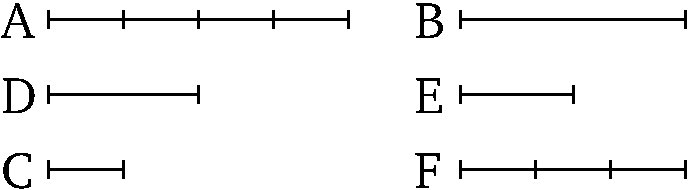
\includegraphics{Book10/fig006e.pdf}}

For let the two magnitudes $A$ and $B$ have to one another the ratio which
the number $D$ (has) to the number $E$. I say that the magnitudes $A$ and $B$ are commensurable.

For, as many units as there are in $D$, let $A$ be divided into so many
equal (divisions). And let $C$ be equal to one of them. And as many
units as there are in $E$, let $F$ be the sum  of so many magnitudes equal to
$C$.

Therefore, since as many units as there are in $D$, so many magnitudes equal to $C$ are also in $A$, therefore whichever part a unit is of $D$, $C$ is also
the same part of $A$. Thus, as $C$ is to $A$, so a unit (is) to $D$ [Def.~7.20]. And a unit measures the number $D$.
Thus, $C$ also measures $A$. And since as $C$ is to $A$, so a unit (is) to
the [number] $D$, thus, inversely, as $A$ (is) to $C$, so the number $D$
(is) to a unit [Prop.~5.7~corr.]. Again, since as many 
units as there are in $E$,  so many (magnitudes) equal to $C$ are also in $F$,
thus as $C$ is to $F$, so a unit (is) to the [number] $E$ [Def.~7.20]. And it was also shown that as $A$ (is) to $C$, so $D$ (is) to a unit. Thus, via equality, as $A$ is to $F$, so $D$ (is)
to $E$ [Prop.~5.22]. But, as $D$ (is) to $E$, 
so $A$ is to $B$. And thus as $A$ (is) to $B$, so (it) also is to $F$ [Prop.~5.11]. Thus,
$A$ has the same ratio to each of $B$ and $F$. Thus, $B$ is equal to
$F$ [Prop.~5.9]. And $C$ measures $F$. Thus,
it also measures $B$. But, in fact, (it) also (measures) $A$. Thus, $C$ measures (both) $A$ and $B$. Thus, $A$ is commensurable with $B$ [Def.~10.1].

Thus,  if two magnitudes \ldots to one another, and so on \ldots.\\

\begin{center}
{\large Corollary}
\end{center}\vspace*{-7pt}

So it is clear, from this, that if there are two numbers, like $D$ and $E$, and
a straight-line, like $A$, then it is possible to contrive that as the number $D$ (is)
to the number $E$, so the straight-line (is) to (another) straight-line ({\rm i.e.,} $F$). And if the mean proportion, (say) $B$,  is taken of $A$ and $F$, 
then as $A$ is to $F$, so the (square) on $A$ (will be) to the (square)
on $B$. That is to say, as the first (is) to the third, so the
(figure) on the first (is) to the similar, and similarly described, (figure) on the second [Prop.~6.19~corr.]. But, as $A$ (is) to
$F$, so the number $D$ is to the number $E$. Thus, it has also been contrived
that as the number $D$ (is) to the number $E$, so the (figure) on the
straight-line $A$ (is) to the (similar figure) on the straight-line $B$. (Which is)
the very thing it was required to show.}
\end{Parallel}

%%%%%%
% Prop 10.7
%%%%%%
\pdfbookmark[1]{Proposition 10.7}{pdf10.7}
\begin{Parallel}{}{} 
\ParallelLText{
\begin{center}
{\large\ggn{7}.}
\end{center}\vspace*{-7pt}

\gr{Τὰ ἀσύμμετρα μεγέθη πρὸξ >άλληλα λόγον οὐκ >έθει, <ὸν ἀριθμὸξ
πρὸξ ἀριθμόν.}

\gr{>'Εστω ἀσύμμετρα μεγέθη τὰ Α, Β; λέγω, <ότι τὸ Α πρὸξ τὸ Β
λόγον οὐκ >έθει, <ὸν ἀριθμὸξ πρὸξ ἀριθμόν.}\\

% Removed epsf size command
\centerline{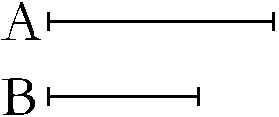
\includegraphics{Book10/fig007g.pdf}}

\gr{Εἰ γὰρ >έθει τὸ Α πρὸξ τὸ Β λόγον, <ὸν ἀριθμὸξ πρὸξ ἀριθμόν,
σύμμετρον >έσται τὸ Α τῶ| Β. οὐκ >έστι δέ; οὐκ >άρα τὸ Α πρὸξ
τὸ Β λόγον >έθει, <ὸν ἀριθμὸξ πρὸξ ἀριθμόν.}

\gr{Τὰ >άρα ἀσύμμετρα μεγέθη πρὸξ >άλληλα λόγον οὐκ >έθει, καὶ
τὰ ἑχῆξ.}}

\ParallelRText{
\begin{center}
{\large Proposition 7}
\end{center}

Incommensurable magnitudes do not
have to one another the ratio which (some) number (has) to (some)
number.

Let $A$ and $B$ be incommensurable magnitudes. I say that $A$ does not
have to $B$ the ratio which (some) number (has) to (some) number.

% Removed epsf size command
\centerline{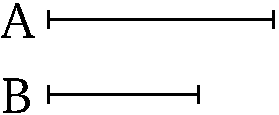
\includegraphics{Book10/fig007e.pdf}}

For if $A$ has to $B$ the ratio which (some) number (has) to (some)
number then $A$ will be commensurable with $B$ [Prop.~10.6]. But it is not. Thus, $A$ does not
have to $B$ the ratio which (some) number (has) to (some) number.

Thus, incommensurable numbers do not have to one another, and
so on \ldots.}
\end{Parallel}

%%%%%%
% Prop 10.8
%%%%%%
\pdfbookmark[1]{Proposition 10.8}{pdf10.8}
\begin{Parallel}{}{} 
\ParallelLText{
\begin{center}
{\large \ggn{8}.}
\end{center}\vspace*{-7pt}

\gr{Ἐὰν δύο μεγέθη πρὸξ >άλληλα λόγον μ\kern -.7pt  ὴ >έθῃ, <ὸν ἀριθμὸξ πρὸξ
ἀριθμόν, ἀσύμμετρα >έσται τὰ μεγέθη.}\\

% Removed epsf size command
\centerline{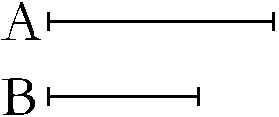
\includegraphics{Book10/fig007g.pdf}}

\gr{Δύο γὰρ μεγέθη τὰ Α, Β πρὸξ >άλληλα λόγον μ\kern -.7pt  ὴ ἐθέτω, <ὸν 
ἀριθμὸξ πρὸξ ἀριθμόν; λέγω, <ότι ἀσύμμετρά ἐστι τὰ Α, Β
μεγέθη.}

\gr{Εἰ γὰρ >έσται σύμμετρα, τὸ Α πρὸξ τὸ Β λόγον <έχει, <ὸν ἀριθμὸξ
πρὸξ ἀριθμόν. οὐκ >έθει δέ. ἀσύμμετρα >άρα ἐστὶ τὰ Α, Β μεγέθη.}

\gr{Ἐὰν >άρα δύο μεγέθη πρὸξ >άλληλα, καὶ τὰ ἑχῆξ.}}

\ParallelRText{
\begin{center}
{\large Proposition 8}
\end{center}

If two magnitudes do not have to one another the
ratio which (some) number (has) to (some) number then the magnitudes
will be incommensurable.

% Removed epsf size command
\centerline{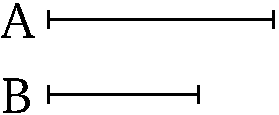
\includegraphics{Book10/fig007e.pdf}}

For let the two magnitudes $A$ and $B$ not have to one another the ratio
which (some) number (has) to (some) number. I say that the magnitudes
$A$ and $B$ are incommensurable.

For if they are commensurable, $A$ will have to $B$ the ratio which (some)
number (has) to (some) number [Prop.~10.5]. But it does not have (such a ratio).
Thus, the magnitudes $A$ and $B$ are incommensurable.

Thus, if two magnitudes \ldots to one another, and so on \ldots.\\~\\}
\end{Parallel}

%%%%%%
% Prop 10.9
%%%%%%
\pdfbookmark[1]{Proposition 10.9}{pdf10.9}
\begin{Parallel}{}{} 
\ParallelLText{
\begin{center}
{\large \ggn{9}.}
\end{center}\vspace*{-7pt}

\gr{Τὰ ἀπὸ τῶν μ\kern -.7pt  ήκει συμμέτρων εὐθειῶν τετράγωνα πρὸξ >άλληλα
λόγον >έθει, <ὸν τετράγωνοξ ἀριθμὸξ πρὸξ τετράγωνον ἀριθμόν;
καὶ τὰ τετράγωνα τὰ πρὸξ >άλληλα λόγον >έθοντα, <ὸν τετράγωνοξ ἀριθμὸξ πρὸξ τετράγωνον ἀριθμόν, καὶ τὰξ πλευρὰξ <έχει μ\kern -.7pt  ήκει
συμμέτρουξ. τὰ δὲ ἀπὸ τῶν μ\kern -.5pt  ήκει ἀσυμμέτρων εὐθειῶν
τετράγωνα πρὸξ >άλληλα λόγον οὐκ >έθει,  <όνπερ
τετράγωνοξ ἀριθμὸξ πρὸξ τετράγωνον ἀριθμόν; καὶ τὰ τετράγωνα
τὰ πρὸξ >άλληλα λόγον μ\kern -.3pt  ὴ >έθοντα, <ὸν τετράγωνοξ ἀριθμὸξ
πρὸξ τετράγωνον ἀριθμόν, οὐδὲ τὰξ πλευρὰξ <έχει μ\kern -.7pt  ήκει
συμμέτρουξ.}\\

% Removed epsf size command
\centerline{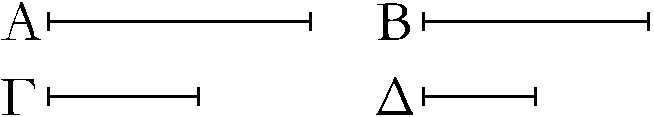
\includegraphics{Book10/fig009g.pdf}}

\gr{>'Εστωσαν γὰρ αἱ Α, Β μ\kern -.7pt  ήκει σύμμετροι; λέγω, <ότι τὸ ἀπὸ τῆξ
Α τετράγωνον πρὸξ τὸ ἀπὸ τῆξ Β τετράγωνον λόγον >έθει,
<ὸν τετράγωνοξ ἀριθμὸξ πρὸξ τετράγωνον ἀριθμόν.}

\gr{Ἐπεὶ γὰρ σύμμετρόξ ἐστιν ἡ Α τῆ| Β μ\kern -.7pt  ήκει, ἡ Α >άρα πρὸξ τὴν
Β λόγον >έθει, <ὸν ἀριθμὸξ πρὸξ ἀριθμόν. ἐθέτω, <ὸν ὁ Γ πρὸξ
τὸν Δ. ἐπεὶ ο>ῦν ἐστιν ὡξ ἡ Α πρὸξ τὴν Β, ο<ύτωξ ὁ Γ
πρὸξ τὸν Δ, ἀλλὰ τοῦ μὲν τῆξ Α πρὸξ τὴν Β λόγου διπλασίων
ἐστὶν ὁ τοῦ ἀπὸ τῆξ Α τετραγώνου πρὸξ τὸ ἀπὸ τῆξ Β τετράγωνον;
τὰ γὰρ <όμοια σθήματα ἐν διπλασίονι λόγῳ ἐστὶ τῶν
ὁμολόγων πλευρῶν; τοῦ δὲ τοῦ Γ [ἀριθμοῦ] πρὸξ τὸν Δ
[ἀριθμὸν] λόγου διπλασίων ἐστὶν ὁ τοῦ ἀπὸ τοῦ Γ
τετραγώνου πρὸξ τὸν ἀπὸ τοῦ Δ τετράγωνον; δύο γὰρ τετραγώνων
ἀριθμῶν ε<ῖξ μέσοξ ἀνάλογόν ἐστιν ἀριθμόξ, καί ὁ τετράγωνοξ
πρὸξ τὸν τετράγωνον [ἀριθμὸν] διπλασίονα λόγον >έθει, >ήπερ
ἡ πλευρὰ πρὸξ τὴν πλευράν; >έστιν >άρα καὶ ὡξ τὸ ἀπὸ τῆξ
Α τετράγωνον πρὸξ τὸ ἀπὸ τῆξ Β τετράγωνον, ο<ύτωξ ὁ 
ἀπὸ τοῦ Γ τετράγωνοξ [ἀριθμὸξ] πρὸξ τὸν ἀπὸ τοῦ Δ [ἀριθμοῦ]
τετράγωνον [ἀριθμόν].}

\gr{Ἀλλὰ δὴ >έστω ὡξ τὸ ἀπὸ τῆξ Α τετράγωνον πρὸξ τὸ ἀπὸ
τῆξ Β, ο<ύτωξ ὁ ἀπὸ τοῦ Γ τετράγωνοξ πρὸξ τὸν ἀπὸ τοῦ
Δ [τετράγωνον]; λέγω, <ότι σύμμετρόξ ἐστιν ἡ Α τῆ| Β μ\kern -.7pt  ήκει.}

\gr{Ἐπεὶ γάρ ἐστιν ὡξ τὸ ἀπὸ τῆξ Α τετράγωνον πρὸξ τὸ ἀπὸ
τῆξ Β [τετράγωνον], ο<ύτωξ ὁ ἀπὸ τοῦ Γ τετράγωνοξ πρὸξ
τὸν ἀπὸ τοῦ Δ [τετράγωνον], ἀλλ> ὁ μὲν τοῦ ἀπὸ τῆξ Α
τετραγώνου πρὸξ τὸ ἀπὸ τῆξ Β [τετράγωνον] λόγοξ
διπλασίων ἐστὶ τοῦ τῆξ Α πρὸξ τὴν Β λόγου, ὁ δὲ τοῦ ἀπὸ τοῦ Γ [ἀριθμοῦ]
τετραγώνου [ἀριθμοῦ] πρὸξ τὸν ἀπὸ τοῦ Δ [ἀριθμοῦ]
τετράγωνον [ἀριθμὸν] λόγοξ διπλασίων ἐστὶ τοῦ τοῦ Γ
[ἀριθμοῦ] πρὸξ τὸν Δ [ἀριθμὸν] λόγου, >έστιν >άρα καὶ ὡξ
ἡ Α πρὸξ τὴν Β, ο<ύτωξ ὁ Γ [ἀριθμὸξ] πρὸξ τὸν Δ [ἀριθμόν]. ἡ Α >άρα πρὸξ τὴν Β λόγον >έθει, <ὸν ἀριθμὸξ ὁ Γ
πρὸξ ἀριθμὸν τὸν Δ; σύμμετροξ >άρα ἐστὶν ἡ Α τῆ| Β μ\kern -.7pt  ήκει.}

\gr{Ἀλλὰ δὴ ἀσύμμετροξ >έστω ἡ Α τῆ| Β μ\kern -.7pt  ήκει; λέγω, <ότι τὸ
ἀπὸ τῆξ Α τετράγωνον πρὸξ τὸ ἀπὸ τῆξ Β [τετράγωνον] λόγον
οὐκ >έθει, <ὸν τετράγωνοξ ἀριθμὸξ πρὸξ τετράγωνον ἀριθμόν.}

\gr{Εἰ γὰρ >έθει τὸ ἀπὸ τῆξ Α τετράγωνον πρὸξ τὸ ἀπὸ τῆξ Β
[τετράγωνον] λόγον, <ὸν τετράγωνοξ ἀριθμὸξ πρὸξ τετράγωνον
ἀριθμόν, σύμμετροξ >έσται ἡ Α τῆ| Β. οὐκ >έστι δέ; οὐκ  >άρα τὸ
ἀπὸ τῆξ Α τετράγωνον πρὸξ τὸ ἀπὸ τῆξ Β [τετράγωνον] λόγον
>έθει, <ὸν τετράγωνοξ ἀριθμὸξ πρὸξ τετράγωνον ἀριθμόν.}

\gr{Πάλιν δὴ τὸ ἀπὸ τῆξ Α τετράγωνον πρὸξ τὸ ἀπὸ τῆξ Β
[τετράγωνον] λόγον μ\kern -.7pt  ὴ ἐθέτω, <ὸν τετράγωνοξ ἀριθμὸξ πρὸξ
τετράγωνον ἀριθμόν; λέγω, <ότι ἀσύμμετρόξ ἐστιν ἡ Α τῆ| Β
μ\kern -.7pt  ήκει.}

\gr{Εἰ γάρ ἐστι σύμμετροξ ἡ Α τῆ| Β, <έχει τὸ ἀπὸ τῆξ Α πρὸξ
τὸ ἀπὸ τῆξ Β λόγον, <ὸν τετράγωνοξ ἀριθμὸξ πρὸξ
τετράγωνον ἀριθμόν. οὐκ >έθει δέ; οὐκ >άρα σύμμετρόξ ἐστιν
ἡ Α τῆ| Β μ\kern -.7pt  ήκει.}

\gr{Τὰ >άρα ἀπὸ τῶν μ\kern -.7pt  ήκει συμμέτρων, καὶ τὰ ἑχῆξ.}\\~\\~\\

\begin{center}
{\large \gr{Πόρισμα}.}
\end{center}

\gr{Καὶ φανερὸν ἐκ τῶν δεδειγμένων >έσται, <ότι αἱ μ\kern -.7pt  ήκει σύμμετροι
πάντωξ καὶ δυνάμει, αἱ δὲ δυνάμει οὐ πάντωξ καὶ μ\kern -.7pt  ήκει.}}

\ParallelRText{
\begin{center}
{\large Proposition 9}
\end{center}

Squares on straight-lines (which are) commensurable in length have to one another the ratio which (some) square number (has) to (some)
square number. And squares having to one another the ratio which (some)
square number (has) to (some) square number will also have sides (which are)
commensurable in length. But squares on straight-lines (which are) incommensurable
in length do not have to one another the ratio which (some) square
number (has) to (some) square number. And squares not having
to one another the ratio which (some) square number (has) to (some)
square number will not have sides (which are) commensurable in length either.

% Removed epsf size command
\centerline{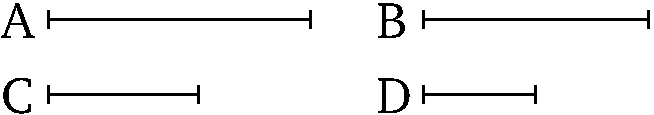
\includegraphics{Book10/fig009e.pdf}}

For let $A$ and $B$ be (straight-lines which are) commensurable in length.
I say that the square on $A$ has to the square on $B$ the ratio
which (some) square number (has) to (some) square number.

For since $A$ is commensurable in length with $B$, $A$ thus
has to $B$ the ratio which (some) number (has) to (some) number [Prop.~10.5]. Let it have (that) which $C$ (has) to $D$.
Therefore, since as $A$ is to $B$, so $C$ (is) to $D$. But the (ratio)
of the square on $A$ to the square on $B$ is the square of the
ratio of $A$ to $B$. For similar figures are in the squared ratio of (their) corresponding sides [Prop.~6.20~corr.].
And the (ratio) of the square on $C$ to the square on $D$ is the
square of the ratio of the [number] $C$ to the [number] $D$.
For there exits one number in mean proportion to two square numbers,
and (one) square (number) has to the (other) square [number] a squared ratio
with respect to (that) the side (of the former has) to the side (of the latter)
[Prop.~8.11]. And, thus,  as the square on $A$
is to the square on $B$, so the square  [number] on the (number) $C$ (is) to
the square [number] on the [number] $D$.$^\dag$

And so let the square on $A$ be to the (square) on $B$ as the
square (number) on $C$ (is) to the [square] (number) on $D$. I say
that $A$ is commensurable in length  with $B$.

For since as the square on $A$ is to the [square] on $B$, so the
square (number) on $C$ (is) to the [square] (number) on $D$. But,
the ratio of the square on $A$ to the (square) on $B$ is the square
of the (ratio) of $A$ to $B$ [Prop.~6.20 corr.].
And the (ratio) of the square [number] on the [number] $C$ to
the square [number] on the [number] $D$ is the square of the ratio
of the [number] $C$ to the [number] $D$ [Prop.~8.11].  Thus, as $A$ is to $B$, so the
[number] $C$ also (is) to the [number] $D$.
$A$, thus,  has to $B$ the ratio
which the number $C$ has to the number $D$. Thus, $A$ is
commensurable in length with $B$ [Prop.~10.6].$^\ddag$

And so let $A$ be incommensurable in length with $B$. I say that
 the square on $A$ does not have to the [square] on $B$ the ratio
which (some) square number (has) to (some) square number.

For if the square on $A$ has to the [square] on $B$ the ratio which
(some) square number (has) to (some) square number then $A$
will be commensurable (in length) with $B$. But it is not. Thus, the square on $A$
does not have to the [square] on the $B$ the ratio which (some)
square number (has) to (some) square number.

So, again, let the square on $A$ not have to the [square] on $B$
the ratio which (some) square number (has) to (some) square number.
I say that $A$ is incommensurable in length with $B$.

For if $A$ is commensurable (in length) with $B$ then  the 
(square) on $A$ will have to the (square) on $B$ the ratio which (some) square
number (has) to (some) square number. But it does not have (such a ratio). 
Thus, $A$ is not commensurable in length with $B$.

Thus, (squares) on (straight-lines which are) commensurable in length,
and so on \ldots.\\

\begin{center}
{\large Corollary}
\end{center}\vspace*{-7pt}

And it will be clear, from (what) has been demonstrated, that (straight-lines)
commensurable in length (are) always also (commensurable) in square, 
but (straight-lines commensurable) in square (are) not always also (commensurable)
in length.}
\end{Parallel}
{\footnotesize\noindent$^\dag$ There is an unstated assumption here that if $\alpha:\beta::\gamma:\delta$ then $\alpha^2:\beta^2::\gamma^2:\delta^2$.\\[0.5ex]
$^\ddag$ There is an unstated
assumption here that if $\alpha^2:\beta^2::\gamma^2:\delta^2$ then $\alpha:\beta::\gamma:\delta$.}

%%%%%%
% Prop 10.10
%%%%%%
\pdfbookmark[1]{Proposition 10.10}{pdf10.10}
\begin{Parallel}{}{} 
\ParallelLText{
\begin{center}
{\large \ggn{10}.}
\end{center}\vspace*{-7pt}

\gr{Τῆ| προτεθείσῃ εὐθείᾳ προσευρεῖν δύο εὐθείαξ ἀσυμμέτ\-ρουξ,
τὴν μὲν μ\kern -.7pt  ήκει μόνον, τὴν δὲ καὶ δυνάμει.}\\

% Removed epsf size command
\centerline{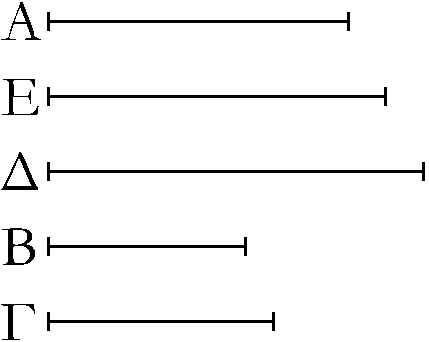
\includegraphics{Book10/fig010g.pdf}}

\gr{>'Εστω ἡ προτεθεῖσα εὐθεῖα ἡ Α; δεῖ δὴ τῆ| Α προσευρεῖν
δύο εὐθείαξ ἀσυμμέτρουξ, τὴν μὲν μ\kern -.7pt  ήκει μόνον, τὴν δὲ
καὶ δυνάμει.}

\gr{Ἐκκείσθωσαν γὰρ δύο αριθμοὶ οἱ Β, Γ πρὸξ ἀλλήλουξ λόγον
μ\kern -.7pt  ὴ >έθοντεξ, <ὸν τετράγωνοξ ἀριθμὸξ πρὸξ τετράγωνον
ἀριθμόν, τουτέστι μ\kern -.7pt  ὴ <όμοιοι ἐπίπεδοι, καὶ γεγονέτω
ὡξ ὁ Β πρὸξ τὸν Γ, ο<ύτωξ τὸ ἀπὸ τῆξ Α τετράγωνον πρὸξ
τὸ ἀπὸ τῆξ Δ τετράγωνον; ἐμάθομεν γάρ; σύμμετρον >άρα τὸ
ἀπὸ τῆξ Α τῶ| ἀπὸ τῆξ Δ. καὶ ἐπεὶ ὁ Β πρὸξ τὸν Γ λόγον
οὐκ >έθει, <ὸν τετράγωνοξ ἀριθμὸξ πρὸξ τετράγωνον ἀριθμόν,
οὐδ> >άρα τὸ ἀπὸ τῆξ Α πρὸξ τὸ ἀπὸ τῆξ Δ λόγον >έθει,
<ὸν τετράγωνοξ ἀριθμὸξ πρὸξ τετράγωνον ἀριθμόν; ἀσύμμετροξ
 >άρα ἐστὶν
ἡ Α τῆ| Δ μ\kern -.5pt  ήκει. εἰλήφθω τῶν Α, Δ μέση ἀνάλογον ἡ Ε; >έστιν
>άρα ὡξ ἡ Α πρὸξ τὴν Δ, ο<ύτωξ τὸ ἀπὸ τῆξ Α τετράγωνον
πρὸξ τὸ ἀπὸ τῆξ Ε. ἀσύμμετροξ δέ ἐστιν ἡ Α τῆ| Δ μ\kern -.3pt  ήκει;
ἀσύμμετρον >άρα ἐστὶ καὶ τὸ ἀπὸ τῆξ Α τετράγωνον
τῶ| ἀπὸ τῆξ Ε τετραγώνῳ; ἀσύμμετροξ >άρα ἐστὶν ἡ Α τῆ|
Ε δυνάμει.}

\gr{Τὴ| >άρα προτεθείσῃ εὐθείᾳ τῆ| Α προσεύρηνται δύο εὐθεῖαι
ἀσύμμετροι αἱ Δ, Ε, μ\kern -.7pt  ήκει μὲν μόνον ἡ Δ,
δυνάμει δὲ καὶ μ\kern -.7pt  ήκει δηλαδὴ ἡ Ε [<όπερ >έδει δεῖχαι].}}

\ParallelRText{
\begin{center}
{\large Proposition 10}$^\dag$
\end{center}

To find two straight-lines incommensurable
with a given straight-line, the one (incommensurable) in length only,
the other also (incommensurable) in square.

% Removed epsf size command
\centerline{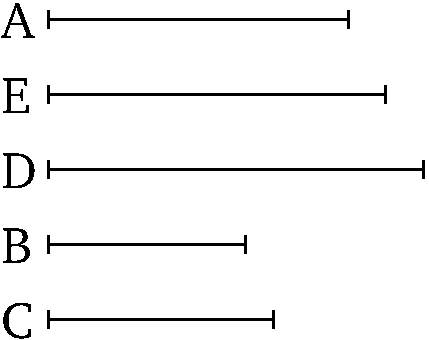
\includegraphics{Book10/fig010e.pdf}}

Let $A$ be the given straight-line. So it is required to find two straight-lines
incommensurable with $A$, the one (incommensurable) in length only,
the other also (incommensurable) in square.

For let two numbers, $B$ and $C$,  not having to one another
the ratio which (some) square number (has) to (some) square number---that
is to say, not (being) similar plane (numbers)---be taken. And let it be contrived
that as $B$ (is) to $C$, so the square on $A$ (is) to the square on $D$.
For we learned (how to do this) [Prop.~10.6 corr.].
Thus, the (square) on $A$ (is) commensurable with the (square) on $D$
[Prop.~10.6]. And since $B$ does not have to $C$ the
ratio which (some) square number (has) to (some) square number, the
(square) on $A$ thus does not have to the (square) on $D$ the ratio which (some) square number (has) to (some) square number either. Thus, $A$ is
incommensurable in length with $D$ [Prop.~10.9].
Let the (straight-line) $E$ (which is) in mean proportion to $A$ and $D$ 
be taken [Prop.~6.13]. Thus, as $A$ is to $D$, so the square on $A$ (is) to the (square)
on $E$ [Def.~5.9]. And $A$ is incommensurable in length with $D$. Thus, the square on $A$ is also incommensurble
with the square on $E$ [Prop.~10.11]. 
Thus, $A$ is incommensurable in square with $E$.

Thus, two straight-lines, $D$ and $E$, (which are) incommensurable with the given
straight-line $A$, be found, the one, $D$, (incommensurable)
in length only, the other, $E$, (incommensurable) in square, and, clearly, also in length. [(Which is) the very thing it was required to show.]}
\end{Parallel}
{\footnotesize\noindent$^\dag$ This whole proposition is regarded by Heiberg as an interpolation into the original text.}

%%%%%%
% Prop 10.11
%%%%%%
\pdfbookmark[1]{Proposition 10.11}{pdf10.11}
\begin{Parallel}{}{} 
\ParallelLText{
\begin{center}
{\large \ggn{11}.}
\end{center}\vspace*{-7pt}

\gr{Ἐὰν τέσσαρα μεγέθη ἀνάλογον >ῆ|, τὸ δὲ πρῶτον τῶ| δευτέρῳ
σύμμετρον >ῆ|, καὶ τὸ τρίτον τῶ| τετάρτῳ σύμμετρον >έσται; κ>ὰν
τὸ πρῶτον τῶ| δευτέρῳ ἀσύμμετρον >ῆ|, καὶ τὸ τρίτον τῶ|
τετάρτῳ ἀσύμμετρον >έσται.}\\

% Removed epsf size command
\centerline{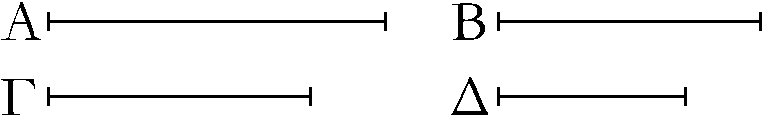
\includegraphics{Book10/fig011g.pdf}}

\gr{>'Εστωσαν τέσσαρα μεγέθη ἀνάλογον τὰ Α, Β, Γ, Δ, ὡξ τὸ Α
πρὸξ τὸ Β, ο<ύτωξ τὸ Γ πρὸξ τὸ Δ, τὸ Α δὲ τῶ| Β σύμμετρον
>έστω; λέγω,  <ότι καὶ τὸ Γ τῶ| Δ σύμμετρον >έσται.}

\gr{Ἐπεὶ γὰρ σύμμετρόν ἐστι τὸ Α τῶ| Β, τὸ Α >άρα πρὸξ τὸ Β
λόγον >έθει, <ὸν ἀριθμὸξ πρὸξ ἀριθμόν. καί ἐστιν ὡξ τὸ Α
πρὸξ τὸ Β, ο<ύτωξ τὸ Γ πρὸξ τὸ Δ; καὶ τὸ Γ >άρα πρὸξ τὸ Δ
λόγον >έθει, <ὸν ἀριθμὸξ πρὸξ ἀριθμόν; σύμμετρον >άρα
ἐστὶ τὸ Γ τῶ| Δ.}

\gr{Ἀλλὰ δὴ τὸ Α τῶ| Β ἀσύμμετρον >έστω; λέγω, <ότι καὶ τὸ
Γ τῶ| Δ ἀσύμμετρον >έσται. ἐπεὶ γὰρ ἀσύμμετρόν ἐστι
τὸ Α τῶ| Β, τὸ Α >άρα πρὸξ τὸ Β λόγον οὐκ >έθει, <ὸν ἀριθμὸξ
πρὸξ ἀριθμόν. καί ἐστιν ὡξ τὸ Α πρὸξ τὸ Β, ο<ύτωξ τὸ Γ πρὸξ τὸ Δ;
οὐδὲ τὸ Γ >άρα πρὸξ τὸ Δ λόγον >έθει, <ὸν ἀριθμὸξ πρὸξ
ἀριθμόν; ἀσύμμετρον >άρα ἐστὶ τὸ Γ τῶ| Δ.}

\gr{Ἐὰν >άρα τέσσαρα μεγέθη, καὶ τὰ ἑχῆξ.}}

\ParallelRText{
\begin{center}
{\large Proposition 11}
\end{center}

If four magnitudes are proportional, and the
first is commensurable with the second, then the third will also be
commensurable with the fourth. And if the first is incommensurable with
the second, then the third will also be incommensurable with the fourth.

% Removed epsf size command
\centerline{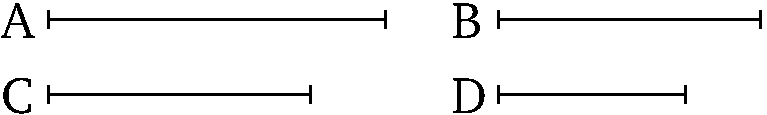
\includegraphics{Book10/fig011e.pdf}}

Let $A$, $B$, $C$, $D$ be four proportional magnitudes, (such that) as
$A$ (is) to $B$, so $C$ (is) to $D$. And let $A$ be commensurable
with $B$. I say that $C$ will also be commensurable with $D$.

For since $A$ is commensurable with $B$, $A$ thus has to $B$ the ratio
which (some) number (has) to (some) number [Prop.~10.5]. And as $A$ is to $B$, so $C$ (is) to $D$. Thus, $C$ also has to $D$ the ratio which (some) number (has) to
(some) number. Thus, $C$ is commensurable with $D$ [Prop.~10.6].

And so let $A$ be incommensurable with $B$. I say that $C$ will also
be incommensurable with $D$. For since $A$ is incommensurable with
$B$, $A$ thus does not have to $B$ the ratio which  (some) number (has) to
(some) number [Prop.~10.7]. And as $A$ is to $B$, so $C$ (is) to $D$. Thus, $C$ does not have to $D$ the ratio which (some) number (has) to
(some) number either. Thus, $C$ is incommensurable with $D$ [Prop.~10.8].

Thus, if four magnitudes, and so on \ldots.}
\end{Parallel}

%%%%%%
% Prop 10.12
%%%%%%
\pdfbookmark[1]{Proposition 10.12}{pdf10.12}
\begin{Parallel}{}{} 
\ParallelLText{
\begin{center}
{\large \ggn{12}.}
\end{center}\vspace*{-7pt}

\gr{Τὰ τῶ| α\kern -.7pt  ὐτῶ| μεγέθει σύμμετρα καὶ ἀλλήλοιξ ἐστὶ σύμμετρα.}

\gr{Ἑκάτερον γὰρ τῶν Α, Β τῶ| Γ >έστω σύμμετρον. λέγω, <ότι
καὶ τὸ Α τῶ| Β ἐστι σύμμετρον.}

\gr{Ἐπεὶ γὰρ σύμμετρόν ἐστι τὸ Α τῶ| Γ, τὸ Α >άρα πρὸξ τὸ Γ λόγον
>έθει, <ὸν ἀριθμὸξ πρὸξ ἀριθμόν. ἐθέτω, <ὸν ὁ Δ πρὸξ τὸν Ε.
πάλιν, ἐπεὶ σύμμετρόν ἐστι τὸ Γ τῶ| Β, τὸ Γ >άρα πρὸξ τὸ Β λόγον
>έθει, <ὸν ἀριθμὸξ πρὸξ ἀριθμόν. ἐθέτω, <ὸν ὁ Ζ πρὸξ τὸν Η.
καὶ λόγων δοθέντων ὁποσωνοῦν τοῦ τε, <ὸν >έθει ὁ Δ πρὸξ τὸν
Ε, καὶ ὁ Ζ πρὸξ τὸν Η εἰλήφθωσαν ἀριθμοὶ ἑχῆξ ἐν τοῖξ δοθεῖσι
λόγοιξ οἱ Θ, Κ, Λ; <ώστε ε>ῖναι ὡξ μὲν τὸν Δ πρὸξ τὸν Ε, ο<ύτωξ
τὸν Θ πρὸξ τὸν Κ, ὡξ δὲ τὸν Ζ πρὸξ τὸν Η, ο<ύτωξ  τὸν Κ πρὸξ τὸν Λ.}\\~\\~\\

% Removed epsf size command
\centerline{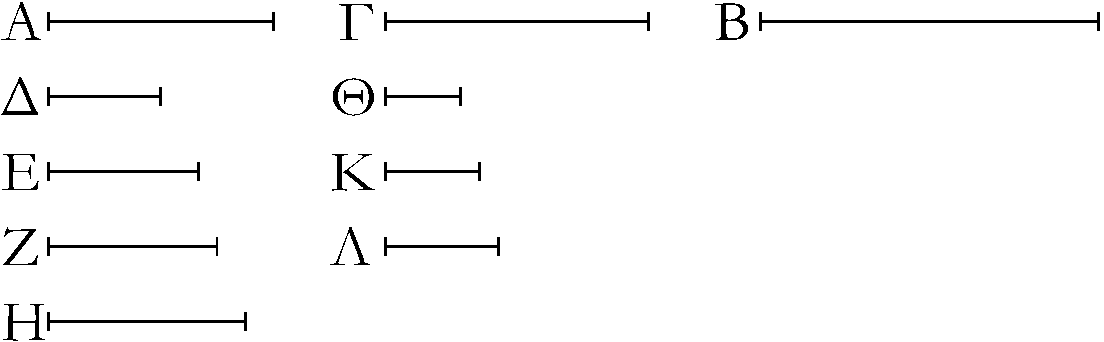
\includegraphics{Book10/fig012g.pdf}}

\gr{Ἐπεὶ ο>ῦν ἐστιν ὡξ τὸ Α πρὸξ τὸ Γ, ο<ύτωξ ὁ Δ πρὸξ τὸν Ε,
ἀλλ> ὡξ ὁ Δ πρὸξ τὸν Ε, ο<ύτωξ ὁ Θ πρὸξ τὸν Κ, >έστιν >άρα
καὶ ὡξ τὸ Α πρὸξ τὸ Γ, ο<ύτωξ ὁ Θ πρὸξ τὸν Κ. πάλιν, ἐπεί ἐστιν
ὡξ τὸ Γ πρὸξ τὸ Β, ο<ύτωξ ὁ Ζ πρὸξ τὸν Η, ἀλλ> ὡξ ὁ Ζ πρὸξ
τὸν Η, [ο<ύτωξ] ὁ Κ πρὸξ τὸν Λ, καὶ ὡξ >άρα τὸ Γ πρὸξ
τὸ Β, ο<ύτωξ ὁ Κ πρὸξ τὸν Λ. >έστι δὲ καὶ ὡξ τὸ Α πρὸξ τὸ
Γ, ο<ύτωξ ὁ Θ πρὸξ τὸν Κ; δι> >ίσου >άρα ἐστὶν ὡξ τὸ Α πρὸξ
τὸ Β, ο<ύτωξ ὁ Θ πρὸξ τὸν Λ. τὸ Α >άρα πρὸξ τὸ Β λόγον
>έθει, <ὸν ἀριθμὸξ ὁ Θ πρὸξ ἀριθμὸν τὸν Λ;
σύμμετρον >άρα ἐστὶ τὸ Α τῶ| Β.}

\gr{Τὰ >άρα τῶ| α\kern -.7pt  ὐτῶ| μεγέθει σύμμετρα καὶ ἀλλήλοιξ ἐστὶ
σύμμετρα; <όπερ >έδει δεῖχαι.}}

\ParallelRText{
\begin{center}
{\large Proposition 12}
\end{center}

(Magnitudes) commensurable with the same magnitude are also commensurable with one another.

For let $A$ and $B$ each be commensurable with $C$. I say that
$A$ is also commensurable with $B$.

For since $A$ is commensurable with $C$, $A$ thus has to $C$ the
ratio which (some) number (has) to (some) number [Prop.~10.5]. Let it have (the ratio) which $D$ (has)
to $E$. Again, since $C$ is commensurable with $B$, $C$ thus has to $B$
the ratio which (some) number (has) to (some) number [Prop.~10.5].  Let it have (the ratio) which $F$ (has) to $G$. And for any multitude whatsoever of given ratios---(namely,) those
which $D$ has to $E$, and $F$ to $G$---let the numbers $H$, $K$, $L$
(which are) continuously (proportional) in the(se) given ratios be taken [Prop.~8.4]. Hence, as $D$ is to $E$, so $H$ (is) to $K$, and as $F$ (is) to $G$, so $K$ (is) to $L$.

% Removed epsf size command
\centerline{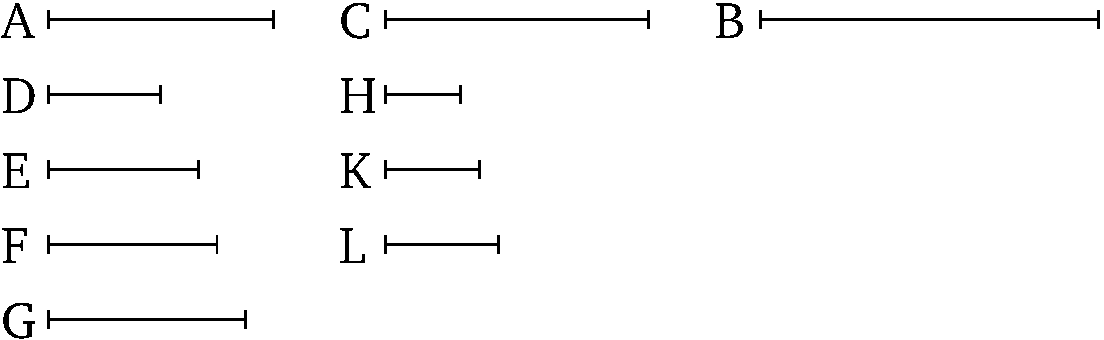
\includegraphics{Book10/fig012e.pdf}}

Therefore, since as $A$ is to $C$, so $D$ (is) to $E$, but as $D$ (is) to 
$E$, so $H$ (is) to $K$, thus also as $A$ is to $C$, so $H$ (is) to $K$
[Prop.~5.11]. Again, since as $C$ is to $B$, 
so $F$ (is) to $G$, but as $F$ (is) to $G$, [so] $K$ (is) to $L$, 
thus also as $C$ (is) to $B$, so $K$ (is) to $L$ [Prop.~5.11]. And also as $A$ is to $C$, so $H$ (is) to $K$. Thus, via equality, as $A$ is to $B$, so $H$ (is) to $L$ [Prop.~5.22]. Thus, $A$ has to $B$ the ratio
which the number $H$ (has) to the number $L$. Thus, $A$ is commensurable
with $B$ [Prop.~10.6].

Thus, (magnitudes) commensurable with the same magnitude are also commensurable with one another. (Which is) the very thing it was required
to show.}
\end{Parallel}

%%%%%%
% Prop 10.13
%%%%%%
\pdfbookmark[1]{Proposition 10.13}{pdf10.13}
\begin{Parallel}{}{} 
\ParallelLText{
\begin{center}
{\large\ggn{13}.}
\end{center}\vspace*{-7pt}

\gr{Ἐὰν >ῆ| δύο μεγέθη σύμμετρα, τὸ δὲ <έτερον α\kern -.7pt  ὐτῶν μεγέθει
τινὶ ἀσύμμετρον >ῆ|, καὶ τὸ λοιπὸν τῶ| α\kern -.7pt  ὐτῶ|
ἀσύμμετρ\-ον >έσται.}\\

% Removed epsf size command
\centerline{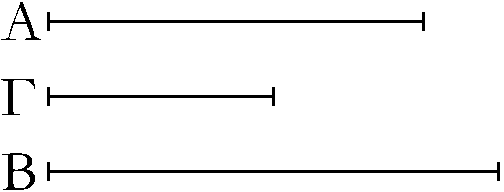
\includegraphics{Book10/fig013g.pdf}}

\gr{>'Εστω δύο μεγέθη σύμμετρα τὰ Α, Β, τὸ δὲ <έτερον α\kern -.7pt  ὐτῶν
τὸ Α >άλλῳ τινὶ τῶ| Γ ἀσύμμετρον >έστω; λέγω, <ότι καὶ τὸ
λοιπὸν τὸ Β τῶ| Γ ἀσύμμετρόν ἐστιν.}

\gr{Εἰ γάρ ἐστι σύμμετρον τὸ Β τῶ| Γ, ἀλλὰ καὶ τὸ Α
τῶ| Β σύμμετρόν ἐστιν, καὶ τὸ Α >άρα τῶ| Γ σύμμετρόν
ἐστιν. ἀλλὰ καὶ ἀσύμμετρον; <όπερ ἀδύνατον. οὐκ >άρα
σύμμετρόν ἐστι τὸ Β τῶ| Γ; ἀσύμμετρον >άρα.}

\gr{Ἐὰν >άρα >ῆ| δύο μεγέθη σύμμετρα, καὶ τὰ ἑχῆξ.}}

\ParallelRText{
\begin{center}
{\large Proposition 13}
\end{center}

If two magnitudes are commensurable, and
one of them is incommensurable  with some magnitude, then the remaining (magnitude)
will also be incommensurable with it.

% Removed epsf size command
\centerline{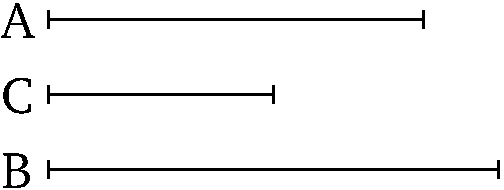
\includegraphics{Book10/fig013e.pdf}}

Let $A$ and $B$ be two commensurable magnitudes, and let one
of them, $A$, be incommensurable with some other (magnitude),
$C$. I say that the remaining (magnitude), $B$, is also incommensurable
with $C$.

For if $B$ is commensurable with $C$, but $A$ is also commensurable
with $B$, $A$ is thus also commensurable with $C$ [Prop.~10.12]. But, (it is) also incommensurable (with
$C$). The very thing (is) impossible. Thus, $B$ is not commensurable
with $C$. Thus, (it is) incommensurable.

Thus, if two magnitudes are commensurable, and so on \ldots.}
\end{Parallel}

%%%%%%
% Prop 10.13a
%%%%%%
\begin{Parallel}{}{} 
\ParallelLText{
\begin{center}
{\large \gr{Λῆμμα}.}
\end{center}\vspace*{-7pt}

\gr{Δύο δοθεισῶν εὐθειῶν ἀνίσων εὑρεῖν, τίνι μεῖζον δύναται
ἡ μείζων τῆξ ἐλάσσονοξ.}\\

% Removed epsf size command
\centerline{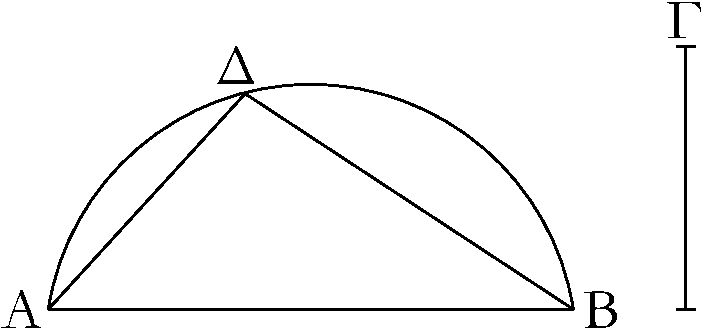
\includegraphics{Book10/fig013ag.pdf}}

\gr{>'Εστωσαν αἱ δοθεῖσαι δύο >άνισοι εὐθεῖαι αἱ ΑΒ, Γ, <ῶν μείζων
>έστω ἡ ΑΒ; δεῖ δὴ εὑρεῖν, τίνι μεῖζον δύναται ἡ ΑΒ τῆξ Γ.}

\gr{Γεγράφθω ἐπὶ τῆξ ΑΒ ἡμικύκλιον τὸ ΑΔΒ, καὶ
εἰξ α\kern -.7pt  ὐτὸ ἐνηρμόσθω τῆ| Γ >ίση ἡ ΑΔ, καὶ ἐπεζεύθθω ἡ ΔΒ.
φανερὸν δή, <ότι ὀρθή ἐστιν ἡ ὑπὸ ΑΔΒ γωνία, καὶ <ότι
ἡ ΑΒ τῆξ ΑΔ, τουτέστι τῆξ Γ, μεῖζον δύναται τῆ| ΔΒ.}

\gr{Ὁμοίωξ δὲ καὶ δύο δοθεισῶν εὐθειῶν ἡ δυναμένη α\kern -.7pt  ὐτὰξ εὑρίσκεται ο<ύτωξ.}

\gr{>'Εστωσαν αἱ δοθεῖσαι δύο εὐθεῖαι αἱ ΑΔ, ΔΒ, καὶ δέον >έστω
εὑρεῖν τὴν δυναμένην α\kern -.7pt  ὐτάξ. κείσθωσαν γάρ, <ώστε ὀρθὴν
γωνίαν περιέθειν τὴν ὑπὸ ΑΔ, ΔΒ, καὶ ἐπεζεύθθω ἡ ΑΒ; φανερὸν
πάλιν, <ότι ἡ τὰξ ΑΔ, ΔΒ δυναμένη ἐστὶν ἡ ΑΒ; <όπερ
>έδει δεῖχαι.}}

\ParallelRText{
\begin{center}
{\large Lemma}
\end{center}

For two given unequal straight-lines, to find by (the square on) which (straight-line)
the square on the greater (straight-line is) larger   than (the square on) the lesser.$^\dag$

% Removed epsf size command
\centerline{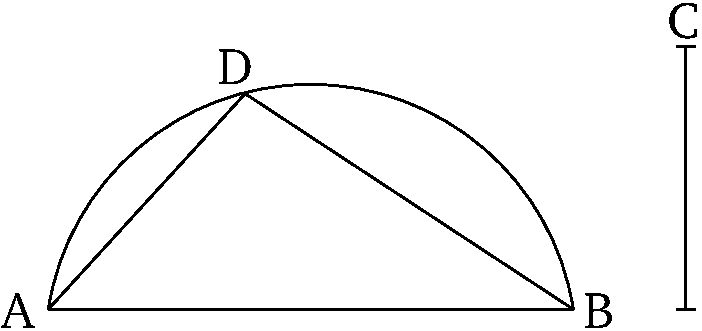
\includegraphics{Book10/fig013ae.pdf}}

Let $AB$ and $C$ be the two given unequal straight-lines, and let $AB$
be the greater of them. So it is required to find by (the square on) which (straight-line)  the square on $AB$ (is) greater  than (the square on) $C$.

Let the semi-circle $ADB$ be described on $AB$.  And let $AD$,
equal to $C$, be inserted into it [Prop.~4.1]. 
And let $DB$ be joined. So (it is) clear that the angle $ADB$
is  a right-angle [Prop.~3.31], and that the square on $AB$
(is) greater than (the square on) $AD$---that is to say, (the square on) $C$---by (the square on) $DB$ [Prop.~1.47].

And, similarly, the square-root of (the sum of the squares on) two given straight-lines
is also found likeso.

Let $AD$ and $DB$ be the two given straight-lines. And let it
be necessary to find the square-root of (the sum of the squares on) them. For let
them be laid down such as to encompass a right-angle---(namely), that (angle encompassed) by
$AD$ and $DB$. And let $AB$ be joined. (It is) again clear that $AB$ is the square-root of   (the sum of the squares on) $AD$ and $DB$ [Prop.~1.47]. (Which is) the very thing it was required to show.}
\end{Parallel}
{\footnotesize\noindent$^\dag$ That is, if $\alpha$ and $\beta$ are the lengths of two given straight-lines, with $\alpha$ being greater
than $\beta$, to find a straight-line of length $\gamma$ such that $\alpha^2=\beta^2+\gamma^2$. Similarly, we can also find $\gamma$
such that $\gamma^2=\alpha^2+\beta^2$.}

%%%%%%
% Prop 10.14
%%%%%%
\pdfbookmark[1]{Proposition 10.14}{pdf10.14}
\begin{Parallel}{}{} 
\ParallelLText{
\begin{center}
{\large \ggn{14}.}
\end{center}\vspace*{-7pt}

\gr{Ἐὰν τέσσαρεξ εὐθεῖαι ἀνάλογον >ῶσιν, δύνηται δὲ ἡ πρώτη
τῆξ δευτέραξ μεῖζον τῶ| ἀπὸ συμμέτρου ἑαυτῆ| [μ\kern -.7pt  ήκει],
καὶ ἡ τρίτη τῆξ τετάρτηξ μεῖζον δυνήσεται τῶ| ἀπὸ συμμέτρου
ἑαυτῆ| [μ\kern -.7pt  ήκει]. καὶ ἒαν ἡ πρώτη τῆξ δευτέραξ μεῖζον δύνηται
τῶ| ἀπὸ ἀσυμμέτρου ἑαυτῆ| [μ\kern -.5pt  ήκει], καὶ ἡ τρίτη τῆξ τετάρτηξ
μεῖζον δυνήσεται τῶ| ἀπὸ ἀσυμμέτρου ἑαυτῆ| [μ\kern -.3pt  ήκει].}

\gr{>'Εστωσαν τέσσαρεξ εὐθεῖαι ἀνάλογον αἱ Α, Β, Γ, Δ, ὡξ ἡ Α
πρὸξ τὴν Β, ο<ύτωξ ἡ Γ πρὸξ τὴν Δ, καὶ ἡ Α μὲν τῆξ Β μεῖζον
δυνάσθω τῶ| ἀπὸ τῆξ Ε, ἡ δὲ Γ τῆξ Δ μεῖζον δυνάσθω
τῶ| ἀπὸ τῆξ Ζ; λέγω, <ότι, ε>ίτε σύμμετρόξ ἐστιν ἡ Α τῆ| Ε,
σύμμετρόξ ἐστι καὶ ἡ Γ τῆ| Ζ, ε>ίτε ἀσύμμετρόξ ἐστιν ἡ Α
τῆ| Ε, ἀσύμμετρόξ ἐστι καὶ ὁ Γ τῆ| Ζ.}\\~\\~\\~\\~\\~\\

% Removed epsf size command
\centerline{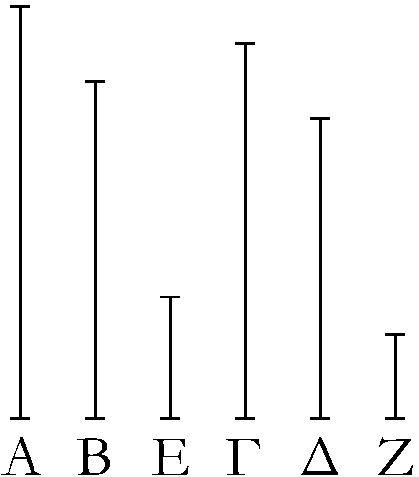
\includegraphics{Book10/fig014g.pdf}}

\gr{Ἐπεὶ γάρ ἐστιν ὡξ ἡ Α πρὸξ τὴν Β, ο<ύτωξ ἡ Γ πρὸξ τὴν
Δ, >έστιν >άρα καὶ ὡξ τὸ ἀπὸ τῆξ Α πρὸξ τὸ ἀπὸ τῆξ Β,
ο<ύτωξ τὸ ἀπὸ τῆξ Γ πρὸξ τὸ ἀπὸ τῆξ Δ. ἀλλὰ τῶ| μὲν
ἀπὸ τῆξ Α >ίσα ἐστὶ τὰ ἀπὸ τῶν Ε, Β, τῶ| δὲ ἀπὸ τῆξ Γ
>ίσα ἐστὶ τὰ ἀπὸ τῶν Δ, Ζ. >έστιν >άρα ὡξ τὰ ἀπὸ τῶν Ε, Β
πρὸξ τὸ ἀπὸ τῆξ Β, ο<ύτωξ τὰ ἀπὸ τῶν Δ, Ζ πρὸξ τὸ ἀπὸ
τῆξ Δ; διελόντι >άρα ἐστὶν ὡξ τὸ ἀπὸ τῆξ Ε πρὸξ τὸ ἀπὸ
τῆξ Β, ο<ύτωξ τὸ ἀπὸ τῆξ Ζ πρὸξ τὸ ἀπὸ τῆξ Δ; >έστιν >άρα
καὶ ὡξ ἡ Ε πρὸξ τὴν Β, ο<ύτωξ ἡ Ζ πρὸξ τὴν Δ; ἀνάπαλιν
>άρα ἐστὶν ὡξ ἡ Β πρὸξ τὴν Ε, ο<ύτωξ ἡ Δ πρὸξ τὴν Ζ. >έστι
δὲ καὶ ὡξ ἡ Α πρὸξ τὴν Β, ο<ύτωξ ἡ Γ πρὸξ τὴν Δ; δι> >ίσου
>άρα ἐστὶν ὡξ ἡ Α πρὸξ τὴν Ε, ο<ύτωξ ἡ Γ πρὸξ τὴν Ζ.
ε>ίτε ο>ῦν σύμμετρόξ ἐστιν ἡ Α τῆ| Ε, συμμετρόξ ἐστι
καὶ ἡ Γ τῆ| Ζ, ε>ίτε ἀσύμμετρόξ ἐστιν ἡ Α τῆ| Ε, ἀσύμμετρόξ
ἐστι καὶ ἡ Γ τῆ| Ζ.}

\gr{Ἐὰν >άρα, καὶ τὰ ἑχῆξ.}}

\ParallelRText{
\begin{center}
{\large Proposition 14}
\end{center}

If four straight-lines are proportional, and the
square on the first is greater  than (the square on) the second  by the (square) on (some straight-line) commensurable [in length] with the first, then the
square on the  third will also
be greater  than (the square on) the fourth by the (square) on (some straight-line) commensurable [in length]
with the third. And if the
square on the first is greater  than (the  square on) the second  by the (square) on (some straight-line) incommensurable [in length] with the first, then the square on the third will also
be greater than (the  square on) the fourth by the (square) on (some straight-line) incommensurable [in length]
with the third. 

Let $A$, $B$, $C$, $D$ be four proportional straight-lines, (such that)
as $A$ (is) to $B$, so $C$ (is) to $D$. And let the square on $A$ be greater 
than (the square on) $B$ by the (square) on $E$, and let the square on $C$ be greater
than (the square on) $D$ by the (square) on $F$. I say that 
$A$ is either commensurable (in length) with $E$, and $C$ is also commensurable with $F$, or $A$ is incommensurable (in length) with $E$, and $C$ is also incommensurable with $F$.

% Removed epsf size command
\centerline{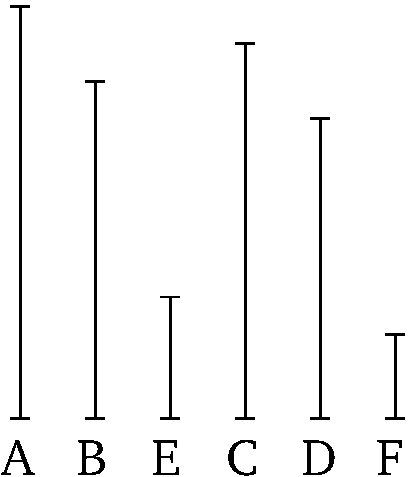
\includegraphics{Book10/fig014e.pdf}}

For since as $A$ is to $B$, so $C$ (is) to $D$, thus as the (square) on $A$
is to the (square) on $B$, so the (square) on $C$  (is) to the (square) on $D$
[Prop.~6.22]. But the (sum of the squares) on $E$ and $B$ is equal to the (square) on $A$, and the (sum of the squares) on 
$D$ and $F$ is equal to the (square) on $C$.
Thus, as the (sum of the squares) on $E$ and $B$ is to the (square) on
$B$, so the (sum of the squares) on $D$ and $F$ (is) to the (square)
on $D$.
 Thus, via separation, as the (square) on $E$ is to the (square) on $B$, so the (square) on $F$ (is) to the (square)
on $D$ [Prop.~5.17]. Thus, also, as $E$ is to $B$,
so $F$ (is) to $D$ [Prop.~6.22]. 
 Thus, inversely,  as $B$ is to $E$, so $D$ (is) to $F$ [Prop.~5.7~corr.]. But, as $A$ is to $B$, so 
 $C$ also (is) to $D$. Thus, via equality, as $A$ is to $E$, so $C$ (is) to $F$
 [Prop.~5.22]. Therefore, $A$ is either commensurable (in length)
 with $E$, and $C$ is also commensurable with $F$, or $A$ is
 incommensurable (in length) with $E$, and $C$ is also incommensurable with $F$ [Prop.~10.11].
 
 Thus, if, and so on \ldots.}
\end{Parallel}

%%%%%%
% Prop 10.15
%%%%%%
\pdfbookmark[1]{Proposition 10.15}{pdf10.15}
\begin{Parallel}{}{} 
\ParallelLText{
\begin{center}
{\large \ggn{15}.}
\end{center}\vspace*{-7pt}

\gr{Ἐὰν δύο μεγέθη σύμμετρα συντεθῆ|, καὶ τὸ <όλον ἑκατέρῳ α\kern -.7pt  ὐτῶν
σύμμετρον >έσται; κ>ὰν τὸ <όλον ἑνὶ α\kern -.7pt  ὐτῶν σύμμετρον >ῆ|, καὶ
τὰ ἐχ ἀρθῆξ μεγέθη σύμμετρα >έσται.}

\gr{Συγκείσθω γὰρ δύο μεγέθη σύμμετρα τὰ ΑΒ, ΒΓ;  λέγω, <ότι καὶ
<όλον τὸ ΑΓ ἑκατέρῳ τῶν ΑΒ, ΒΓ ἐστι σύμμετρον.}\\~\\~\\

% Removed epsf size command
\centerline{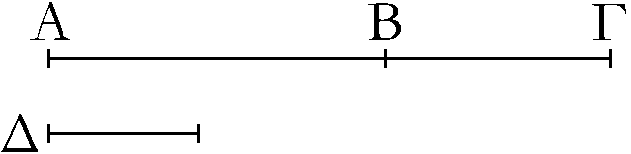
\includegraphics{Book10/fig015g.pdf}}

\gr{Ἐπεὶ γὰρ σύμμετρά ἐστι τὰ ΑΒ, ΒΓ, μετρήσει τι α\kern -.7pt  ὐτὰ μέγεθοξ.
μετρείτω, καὶ >έστω τὸ Δ. ἐπεὶ ο>ῦν τὸ Δ τὰ ΑΒ, ΒΓ μετρεῖ,
καὶ <όλον τὸ ΑΓ μετρήσει. μετρεῖ δὲ καὶ τὰ ΑΒ, ΒΓ. τὸ Δ >άρα
τὰ ΑΒ, ΒΓ, ΑΓ μετρεῖ; σύμμετρον >άρα ἐστὶ τὸ ΑΓ ἑκατέρῳ
τῶν ΑΒ, ΒΓ.}

\gr{Ἀλλὰ δὴ τὸ ΑΓ >έστω σύμμετρον τῶ| ΑΒ; λέγω δή, <ότι καὶ τὰ
ΑΒ, ΒΓ σύμμετρά ἐστιν.}

\gr{Ἐπεὶ γὰρ σύμμετρά ἐστι τὰ ΑΓ, ΑΒ, μετρήσει τι α\kern -.7pt  ὐτὰ μέγεθοξ.
μετρείτω, καὶ >έστω τὸ Δ. ἐπεὶ ο>ῦν τὸ Δ τὰ ΓΑ, ΑΒ
μετρεῖ, καὶ λοιπὸν >άρα τὸ ΒΓ μετρήσει. μετρεῖ δὲ καὶ τὸ ΑΒ;
τὸ Δ >άρα τὰ ΑΒ, ΒΓ μετρήσει; σύμμετρα >άρα ἐστὶ τὰ ΑΒ, ΒΓ.}

\gr{Ἐὰν >άρα δύο μεγέθη, καὶ τὰ ἑχῆξ.}}

\ParallelRText{
\begin{center}
{\large Proposition 15}
\end{center}

If two commensurable magnitudes are
added together then the whole will also be commensurable
with each of them. And if the whole is commensurable with one of
them then the original magnitudes will also be commensurable (with one another).

For let the two commensurable magnitudes $AB$ and $BC$ be laid
down together. I say that the whole $AC$ is also commensurable with
each of $AB$ and $BC$.

% Removed epsf size command
\centerline{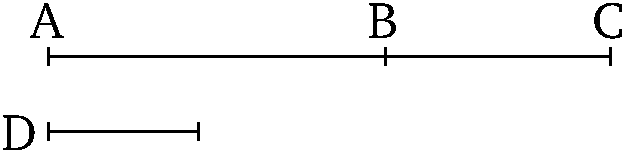
\includegraphics{Book10/fig015e.pdf}}

For since $AB$ and $BC$ are commensurable, some  magnitude will
measure them. Let it (so) measure (them), and let it be $D$. Therefore,
since $D$ measures (both) $AB$ and $BC$, it will also measure the
whole $AC$. And it also measures $AB$ and $BC$. Thus, $D$
measures  $AB$, $BC$, and $AC$. Thus, $AC$ is commensurable
with each of $AB$ and $BC$ [Def.~10.1].

And so let $AC$ be commensurable with $AB$. I say that $AB$ and
$BC$ are also commensurable.

For since $AC$ and $AB$ are commensurable, some  magnitude
will measure them. Let it (so) measure (them), and let it be $D$. Therefore,
since $D$ measures (both) $CA$ and $AB$, it will thus also
measure the remainder $BC$. And it also measures $AB$. Thus, $D$ will
measure (both) $AB$ and $BC$. Thus, $AB$ and $BC$ are commensurable [Def.~10.1].

Thus, if two magnitudes, and so on \ldots.}
\end{Parallel}

%%%%%%
% Prop 10.16
%%%%%%
\pdfbookmark[1]{Proposition 10.16}{pdf10.16}
\begin{Parallel}{}{} 
\ParallelLText{
\begin{center}
{\large \ggn{16}.}
\end{center}\vspace*{-7pt}

\gr{Ἐὰν δύο μεγέθη ἀσύμμετρα συντεθῆ|, καὶ τὸ <όλον ἑκατέρῳ
α\kern -.7pt  ὐτῶν ἀσύμμετρον >έσται; κ>ὰν τὸ <όλον ἑνὶ α\kern -.7pt  ὐτῶν
ἀσύμμετρον >ῆ|, καὶ τὰ ἐχ ἀρθῆξ μεγέθη ἀσύμμετρα >έσται.}\\~\\

% Removed epsf size command
\centerline{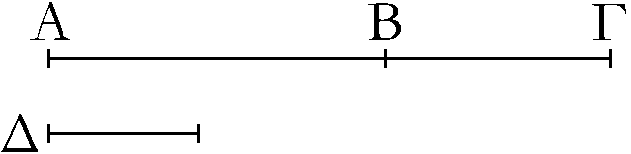
\includegraphics{Book10/fig015g.pdf}}

\gr{Συγκείσθω γὰρ δύο μεγέθη ἀσύμμετρα τὰ ΑΒ, ΒΓ; λέγω, <ότι
καὶ <όλον τὸ ΑΓ ἑκατέρῳ τῶν ΑΒ, ΒΓ ἀσύμμετρόν ἐστιν.}

\gr{Εἰ γὰρ μ\kern -.7pt  ή ἐστιν ἀσύμμετρα τὰ ΓΑ, ΑΒ, μετρήσει τι [α\kern -.7pt  ὐτὰ]
μέγεθοξ. μετρείτω, εἰ δυνατόν, καὶ >έστω τὸ Δ. ἐπεὶ ο>ῦν
τὸ Δ τὰ ΓΑ, ΑΒ μετρεῖ, καὶ λοιπὸν >άρα τὸ ΒΓ μετρήσει. μετρεῖ
δὲ καὶ τὸ ΑΒ; τὸ Δ >άρα τὰ ΑΒ, ΒΓ μετρεῖ. σύμμετρα >άρα ἐστὶ
τὰ ΑΒ, ΒΓ; ὑπέκειντο δὲ καὶ ἀσύμμετρα; <όπερ ἐστὶν ἀδύνατον.
οὐκ >άρα τὰ ΓΑ, ΑΒ μετρήσει τι μέγεθοξ; ἀσύμμετρα >άρα
ἐστὶ τὰ ΓΑ, ΑΒ. ὁμοίωξ δὴ δείχομεν,  <ότι καὶ τὰ ΑΓ, ΓΒ
ἀσύμμετρά ἐστιν. τὸ ΑΓ >άρα ἑκατέρῳ τῶν ΑΒ, ΒΓ ἀσύμμετρόν
ἐστιν.}

\gr{Ἀλλὰ δὴ τὸ ΑΓ ἑνὶ τῶν ΑΒ, ΒΓ ἀσύμμετρον >έστω. >έστω δὴ
πρότερον τῶ| ΑΒ; λέγω, <ότι καὶ τὰ ΑΒ, ΒΓ ἀσύμμετρά ἐστιν.
εἰ γὰρ >έσται σύμμετρα, μετρήσει τι α\kern -.7pt  ὐτὰ μέγεθοξ. μετρείτω,
καὶ >έστω τὸ Δ. ἐπεὶ ο>ῦν τὸ Δ τὰ ΑΒ, ΒΓ μετρεῖ, καὶ
<όλον >άρα τὸ ΑΓ μετρήσει. μετρεῖ δὲ καὶ τὸ ΑΒ; τὸ Δ >άρα
τὰ ΓΑ, ΑΒ μετρεῖ. σύμμετρα >άρα ἐστὶ τὰ ΓΑ, ΑΒ; ὑπέκειτο
δὲ καὶ ἀσύμμετρα; <όπερ ἐστὶν ἀδύνατον. οὐκ >άρα τὰ ΑΒ, ΒΓ
μετρήσει τι μέγεθοξ; ἀσύμμετρα >άρα ἐστὶ τὰ ΑΒ, ΒΓ.}

\gr{Ἐὰν >άρα δύο μεγέθη, καὶ τὰ ἑχῆξ.}}

\ParallelRText{
\begin{center}
{\large Proposition 16}
\end{center}

If two incommensurable magnitudes are
added together then the whole will also be incommensurable with
each of them. And if the whole is incommensurable with one of them then
the original magnitudes will also be incommensurable (with one another).

% Removed epsf size command
\centerline{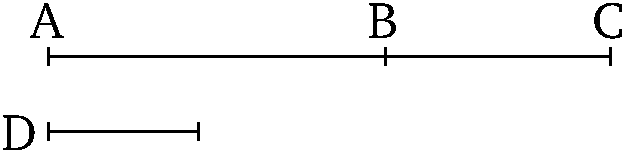
\includegraphics{Book10/fig015e.pdf}}

For let the two incommensurable magnitudes $AB$ and $BC$ be
laid down together. I say that that the whole $AC$ is also
incommensurable with each of $AB$ and $BC$.

For if $CA$ and $AB$ are not incommensurable then some magnitude
will measure [them]. If possible, let it (so) measure (them), and let it
be $D$. Therefore, since $D$ measures (both) $CA$ and $AB$, it will
thus also measure the remainder $BC$. And it also measures $AB$.
Thus, $D$ measures (both) $AB$ and $BC$. Thus, $AB$ and $BC$ are
commensurable [Def.~10.1]. But they were also assumed (to be) incommensurable.
The very thing is impossible. Thus, some magnitude cannot
measure (both) $CA$ and $AB$. Thus, $CA$ and $AB$ are incommensurable [Def.~10.1]. So, similarly, we can show that $AC$ and
$CB$ are also incommensurable. Thus, $AC$ is incommensurable with each
of $AB$ and $BC$.

And so let $AC$ be incommensurable with one of $AB$ and $BC$. So
let it, first of all, be incommensurable with $AB$. I say that $AB$ and
$BC$ are also incommensurable. For if they are commensurable then
some magnitude will measure them. Let it (so) measure (them), and let it
be $D$. Therefore, since $D$ measures (both) $AB$ and $BC$, 
it will thus also measure the whole  $AC$. And it also measures $AB$. 
Thus, $D$ measures (both) $CA$ and $AB$. Thus, $CA$ and $AB$
are commensurable  [Def.~10.1]. But they
were also assumed (to be) incommensurable. The very thing is
impossible. Thus, some magnitude cannot measure (both) $AB$ and
$BC$. Thus, $AB$ and $BC$ are incommensurable  [Def.~10.1].

Thus, if two\ldots magnitudes, and so on \ldots.}
\end{Parallel}

%%%%%%
% Prop 10.16a
%%%%%%
\begin{Parallel}{}{} 
\ParallelLText{
\begin{center}
{\large \gr{Λῆμμα}.}
\end{center}\vspace*{-7pt}

\gr{Ἐὰν παρά τινα εὐθεῖαν παραβληθῆ| παραλληλόγραμ\-μον ἐλλεῖπον
ε>ίδει τετραγώνῳ, τὸ παραβληθὲν >ίσον ἐστὶ τῶ| ὑπὸ τῶν
ἐκ τῆξ παραβολήξ γενομένων τμ\kern -.7pt  ημάτων τῆξ εὐθείαξ.}\\

% Removed epsf size command
\centerline{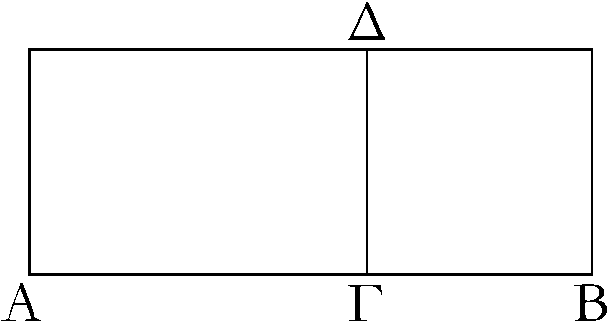
\includegraphics{Book10/fig016ag.pdf}}

\gr{Παρὰ γὰρ εὐθεῖαν τὴν ΑΒ παραβεβλήσθω παραλληλόγραμμον τὸ
ΑΔ ἐλλεῖπον ε>ίδει τετραγώνῳ τῶ| ΔΒ;
λέγω, <ότι >ίσον ἐστὶ τὸ ΑΔ τῶ| ὑπὸ τῶν ΑΓ, ΓΒ.}

\gr{Καί ἐστιν α\kern -.7pt  ὐτόθεν φανερόν; ἐπεὶ γὰρ τετράγωνόν ἐστι τὸ ΔΒ,
>ίση ἐστὶν ἡ ΔΓ τῆ| ΓΒ, καί ἐστι τὸ ΑΔ τὸ ὑπὸ τῶν
ΑΓ, ΓΔ, τουτέστι τὸ ὑπὸ τῶν ΑΓ, ΓΒ.}

\gr{Ἐὰν >άρα παρά τινα εὐθεῖαν, καὶ τὰ ἑχῆξ.}}

\ParallelRText{
\begin{center}
{\large Lemma}
\end{center}

If a parallelogram,$^\dag$
 falling short by a square figure, is applied to some straight-line then the applied (parallelogram) is equal (in area) to the (rectangle contained) by the
pieces of the straight-line created via the application (of the parallelogram).

% Removed epsf size command
\centerline{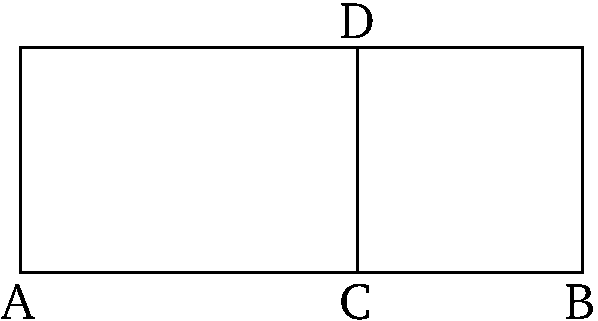
\includegraphics{Book10/fig016ae.pdf}}

For let the parallelogram $AD$, falling short by the square figure $DB$, be applied to the straight-line $AB$. I say that $AD$ is equal to
the (rectangle contained) by $AC$ and $CB$.

And it is immediately obvious. For since $DB$ is a square, $DC$ is
equal to $CB$. And $AD$ is the (rectangle contained) by $AC$ and
$CD$---that is to say, by $AC$ and $CB$.

Thus, if \ldots to some straight-line, and so on \ldots.}
\end{Parallel}
{\footnotesize\noindent$^\dag$  Note that this lemma only applies to rectangular parallelograms.}

%%%%%%
% Prop 10.17
%%%%%%
\pdfbookmark[1]{Proposition 10.17}{pdf10.17}
\begin{Parallel}{}{} 
\ParallelLText{
\begin{center}
{\large \ggn{17}.}
\end{center}\vspace*{-7pt}

\gr{Ἐὰν >ῶσι δύο εὐθεῖαι >άνισοι, τῶ| δὲ τετράτῳ μέρει τοῦ ἀπὸ
τῆξ ἐλάσσονοξ >ίσον παρὰ τὴν μείζονα παραβληθῆ| ἐλλεῖπον
ε>ίδει τετραγώνῳ καὶ εἰξ σύμμετρα α\kern -.7pt  ὐτὴν διαιρῆ| μ\kern -.7pt  ήκει, ἡ
μείζων τῆξ ἐλάσσονοξ μεῖζον δυνήσεται τῶ| ἀπὸ συμμέτου
ἑαυτῆ| [μ\kern -.5pt  ήκει]. καὶ ἒαν ἡ μείζων τῆξ ἐλάσσονοξ μεῖζον
δύνηται τῶ| ἀπὸ συμμέτρου ἑαυτῆ| [μ\kern -.3pt  ήκει], τῶ| δὲ τετράρτῳ τοῦ
ἀπὸ τῆξ ἐλάσσονοξ >ίσον παρὰ τὴν μείζονα παραβληθῆ| ἐλλεῖπον
ε>ίδει τετραγώνῳ, εἰξ σύμμετρα α\kern -.7pt  ὐτὴν διαιρεῖ μ\kern -.7pt  ήκει.}

\gr{>'Εστωσαν δύο εὐθεῖαι >άνισοι αἱ Α, ΒΓ, <ῶν μείζων
ἡ ΒΓ, τῶ| δὲ τετράρτῳ μέρει τοῦ ἀπὸ ἐλάσσονοξ
τῆξ Α, τουτέστι τῶ| ἀπὸ τῆξ ἡμισείαξ τῆξ Α, >ίσον παρὰ
τὴν ΒΓ παραβεβλήσθω ἐλλεῖπον ε>ίδει τετραγώνῳ, καὶ >έστω
τὸ ὑπὸ τῶν ΒΔ, ΔΓ, σύμμετροξ δὲ >έστω ἡ ΒΔ τῆ| ΔΓ
μ\kern -.7pt  ήκει; λέγω, <ὸτι ἡ ΒΓ τῆξ Α μεῖζον δύναται τῶ| ἀπὸ
συμμέτρου ἑαυτῆ|.}\\~\\~\\~\\~\\~\\~\\~\\

% Removed epsf size command
\centerline{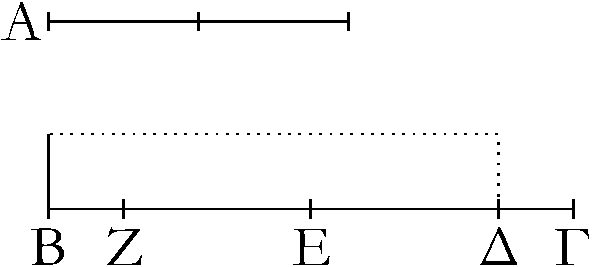
\includegraphics{Book10/fig017g.pdf}}

\gr{Τετμ\kern -.7pt  ήσθω γὰρ ἡ ΒΓ δίθα κατὰ τὸ Ε σημεῖον, καὶ κείσθω τῆ| ΔΕ
>ίση ἡ ΕΖ. λοιπὴ >άρα ἡ ΔΓ >ίση ἐστὶ τῆ| ΒΖ. καὶ ἐπεὶ εὐθεῖα
ἡ ΒΓ τέτμ\kern -.7pt  ηται εἰξ μὲν >ίσα κατὰ τὸ Ε, εἰξ δὲ >άνισα κατὰ τὸ Δ,
τὸ >άρα ὑπὸ ΒΔ, ΔΓ περειθόμενον ὀρθογώνιον μετὰ τοῦ ἀπὸ
τῆξ ΕΔ τετραγώνου >ίσον ἐστὶ τῶ| ἀπὸ τῆξ ΕΓ τετραγώνῳ;
καὶ τὰ τετραπλάσια; τὸ >άρα τετράκιξ ὑπὸ τῶν ΒΔ, ΔΓ μετὰ τοῦ
τετραπλασίου τοῦ ἀπὸ τῆξ ΔΕ >ίσον ἐστὶ τῶ| τετράκιξ ἀπὸ
τῆξ ΕΓ τετραγώνῳ.
ἀλλὰ τῶ| μὲν τετραπλασίῳ τοῦ ὑπὸ τῶν ΒΔ, ΔΓ >ίσον ἐστὶ
τὸ ἀπὸ τῆξ Α τετράγωνον, τῶ| δὲ τετραπλασίῳ τοῦ ἀπὸ τῆξ
ΔΕ >ίσον ἐστὶ τὸ ἀπὸ τῆξ ΔΖ τετράγωνον; διπλασίων γάρ
ἐστιν ἡ ΔΖ τῆξ ΔΕ. τῶ| δὲ τετραπλασίῳ τοῦ ἀπὸ τῆξ ΕΓ >ίσον
ἐστὶ τὸ ἀπὸ τῆξ ΒΓ τετράγωνον; διπλασίων γάρ ἐστι πάλιν
ἡ ΒΓ τῆξ ΓΕ. τὰ >άρα ἀπὸ τῶν Α, ΔΖ τετράγωνα >ίσα ἐστὶ
τῶ| ἀπὸ τῆξ ΒΓ τετράγωνῳ; <ώστε τὸ ἀπὸ τῆξ ΒΓ τοῦ ἀπὸ
τῆξ Α μεῖζόν ἐστι τῶ| ἀπὸ τῆξ ΔΖ; ἡ ΒΓ >άρα τῆξ Α μεῖζον
δύναται τῆ| ΔΖ. δεικτέον, <ότι καὶ σύμμετρόξ ἐστιν ἡ ΒΓ τῆ|
ΔΖ. ἐπεὶ γὰρ σύμμετρόξ ἐστιν ἡ ΒΔ τῆ|
ΔΓ μ\kern -.5pt  ήκει, σύμμετροξ >άρα ἐστὶ καὶ ἡ ΒΓ τῆ| ΓΔ μ\kern -.3pt  ήκει. ἀλλὰ
ἡ ΓΔ ταῖξ ΓΔ, ΒΖ ἐστι σύμμετροξ μ\kern -.7pt  ήκει; >ίση γάρ
ἐστιν ἡ ΓΔ τῆ| ΒΖ. καὶ ἡ ΒΓ >άρα σύμμετρόξ ἐστι ταῖξ ΒΖ, ΓΔ
μ\kern -.7pt  ήκει; <ώστε καὶ λοιπῆ| τῆ| ΖΔ σύμμετρόξ ἐστιν ἡ ΒΓ μ\kern -.7pt  ήκει;
ἡ ΒΓ >άρα τῆξ Α μεῖζον δύναται τῶ| ἀπὸ
συμμέτρου ἑαυτῆ|.}

\gr{Ἀλλὰ δὴ ἡ ΒΓ τῆξ Α μεῖζον δυνάσθω τῶ| ἀπὸ συμμέτρου
ἑαυτῆ|, τῶ| δὲ τετράτρῳ τοῦ ἀπὸ τῆξ Α >ίσον παρὰ τὴν ΒΓ
παραβεβλήσθω ἐλλεῖπον ε>ίδει τετραγώνῳ, καὶ >έστω τὸ ὑπὸ
τῶν ΒΔ, ΔΓ. δεικτέον, <ότι σύμμετρόξ ἐστιν ἡ ΒΔ τῆ| ΔΓ
μ\kern -.7pt  ήκει.}

\gr{Τῶν γὰρ α\kern -.7pt  ὐτῶν κατασκευασθέντων ὁμοίωξ δείχομεν, <ότι
ἡ ΒΓ τῆξ Α μεῖζον δύναται τῶ| ἀπὸ τῆξ ΖΔ.
δύναται δὲ ἡ ΒΓ τῆξ Α μεῖζον τῶ| ἀπὸ συμμέτρου ἑαυτῆ|.
σύμμετροξ >άρα ἐστὶν ἡ ΒΓ τῆ| ΖΔ μ\kern -.7pt  ήκει;
<ώστε καὶ λοιπῆ| συναμφοτέρῳ τῆ| ΒΖ, ΔΓ σύμμετρόξ
ἐστιν ἡ ΒΓ μ\kern -.5pt  ήκει. ἀλλὰ συναμφότεροξ ἡ ΒΖ, ΔΓ σύμμετρόξ
ἐστι τῆ| ΔΓ [μ\kern -.3pt  ήκει]. <ώστε καὶ ἡ ΒΓ τῆ| ΓΔ σύμμετρόξ
ἐστι μ\kern -.7pt  ήκει; καὶ διελόντι >άρα ἡ ΒΔ τῆ| ΔΓ ἐστι σύμμετροξ
μ\kern -.7pt  ήκει.}

\gr{Ἐὰν >άρα >ῶσι δύο εὐθεῖαι >άνισοι, καὶ τὰ ἑχῆξ.}}

\ParallelRText{
\begin{center}
{\large Proposition 17}$^\dag$
\end{center}

If there are two unequal straight-lines,
and a (rectangle) equal to the fourth part of the (square) on the
lesser, falling short by a square figure, is applied to the greater, and
divides it into (parts which are) commensurable in length, then
 the  square on the greater  will be  larger than (the  square on) the lesser  by the (square)
on (some straight-line) commensurable [in length] with the greater.
And if the square on the greater is larger than (the square on) the lesser  by the (square)
on (some straight-line) commensurable [in length] with the greater, and
a (rectangle) equal to the fourth (part) of the (square) on the lesser,
falling short by a square figure, is applied to the greater, then it divides it into (parts
which are) commensurable in length.

Let $A$ and $BC$ be two unequal straight-lines, of which (let) $BC$ (be) the
greater. And let a (rectangle) equal to the fourth part of the (square) on the
lesser, $A$---that is, (equal) to the (square) on half of $A$---falling short by a
square figure, be applied to $BC$. And let it be the (rectangle contained) by $BD$ and $DC$ [see previous lemma]. And let $BD$ be commensurable in length with
$DC$. I say that that the square on $BC$ is greater than the (square on) $A$ by (the square on some straight-line) commensurable (in length) with ($BC$).

% Removed epsf size command
\centerline{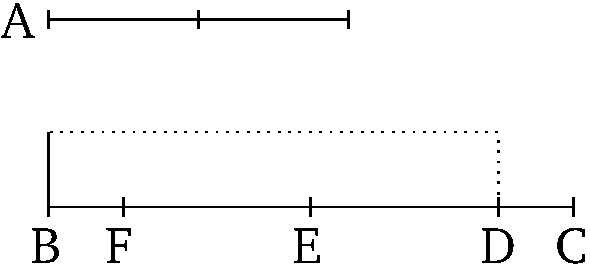
\includegraphics{Book10/fig017e.pdf}}

For let $BC$ be cut in  half at the point $E$ [Prop. 1.10]. And let $EF$ be made equal to
$DE$ [Prop.~1.3]. Thus, the remainder $DC$
is equal to $BF$. And since the straight-line $BC$ has been cut into equal
(pieces) at $E$, and into unequal (pieces) at $D$, the rectangle contained by
$BD$ and $DC$, plus the square on $ED$, is thus equal to the square on $EC$ [Prop.~2.5]. (The same) also (for) the quadruples.  
Thus, four times the (rectangle contained) by $BD$ and $DC$, plus
the quadruple of the (square) on $DE$, is equal to four times the square on 
$EC$. But, the square on $A$ is equal to the quadruple of the (rectangle
contained) by $BD$ and $DC$, and the square on $DF$ is equal to
the quadruple of the (square) on $DE$. For $DF$ is double $DE$. 
And the square on  $BC$ is equal to the quadruple of the (square) on $EC$.
For, again, $BC$ is double $CE$. Thus, the (sum of the) squares on $A$ and
$DF$ is equal to the square on $BC$. Hence, the (square) on $BC$
is greater than the (square) on $A$ by the (square) on $DF$. Thus,
$BC$ is greater in square than $A$ by $DF$. It must also be shown that $BC$
is commensurable (in length) with $DF$. For since $BD$ is commensurable in length
with $DC$, $BC$ is thus also commensurable in length with $CD$ [Prop.~10.15]. 
But, $CD$ is commensurable in length with $CD$ plus $BF$. For $CD$ is equal
to $BF$ [Prop.~10.6].  Thus, $BC$ is also commensurable in length with $BF$ plus $CD$
[Prop.~10.12]. Hence, $BC$ is also commensurable
in length with the remainder $FD$ [Prop.~10.15]. Thus, the square on $BC$ is
greater than (the square on) $A$ by the (square) on (some straight-line)
commensurable (in length) with ($BC$).

And so let the square on $BC$ be greater than the (square on) $A$ by the
(square) on (some straight-line) commensurable (in length) with ($BC$). And let
a (rectangle) equal to the fourth (part) of the (square) on $A$, falling
short by a square figure, be applied to $BC$. And let it be
the (rectangle contained) by $BD$ and $DC$. It must be shown that $BD$
is commensurable in length with $DC$.

For, similarly, by the same construction, we can  show that the
square on $BC$ is greater than the (square on) $A$ by the (square) on $FD$.
And the square on $BC$ is greater than the (square on) $A$ by the
(square) on (some straight-line) commensurable (in length) with ($BC$).  Thus, $BC$ is
commensurable in length with $FD$. Hence, $BC$ is also commensurable in length with the remaining sum of $BF$ and $DC$ [Prop.~10.15]. But, the sum of $BF$ and $DC$
is commensurable [in length] with $DC$ [Prop.~10.6]. Hence, $BC$ is also
commensurable in length with $CD$ [Prop.~10.12]. 
Thus, via separation, $BD$ is also commensurable in length with $DC$ [Prop.~10.15].

Thus,  if there are two unequal straight-lines, and so on \ldots.}
\end{Parallel}
{\footnotesize\noindent$^\dag$ This proposition states that if $\alpha\,x-x^2=\beta^2/4$ (where $\alpha=BC$, $x=DC$,
and $\beta=A$) then $\alpha$ and $\sqrt{\alpha^2-\beta^2}$ are commensurable when $\alpha-x$ are $x$ are commensurable, and {\rm vice versa}.}

%%%%%%
% Prop 10.18
%%%%%%
\pdfbookmark[1]{Proposition 10.18}{pdf10.18}
\begin{Parallel}{}{} 
\ParallelLText{
\begin{center}
{\large\ggn{18}.}
\end{center}\vspace*{-7pt}

\gr{Ἐὰν >ῶσι δύο εὐθεῖαι >άνισοι, τῶ| δὲ τετάρτῳ μέρει τοῦ ἀπὸ
τῆξ ἐλάσσονοξ >ίσον παρὰ τὴν μείζονα παραβληθῆ| ἐλλεῖπον ε>ίδει
τετραγώνῳ, καὶ εἰξ ἀσυμμετρα α\kern -.7pt  ὐτὴν διαιρῆ| [μ\kern -.7pt  ήκει], ἡ μείζων
τῆξ ἐλάσσονοξ μεῖζον δυνήσεται τῶ| ἀπὸ ἀσυμμέτρου ἑαυτῆ|.
καὶ ἒαν ἡ μείζων τῆξ ἐλάσσονοξ μεῖζον δύνηται τῶ| ἀπὸ
ἀσυμμέτρου ἑαυτῆ|, τῶ| δὲ τετράρτῳ τοῦ ἀπὸ τῆξ ἐλάσσονοξ
>ίσον παρὰ τὴν μείζονα παραβληθῆ| ἐλλεῖπον ε>ίδει τετραγώνῳ,
εἰξ ἀσύμμετρα α\kern -.5pt  ὐτὴν διαιρεῖ [μ\kern -.3pt  ήκει].}

\gr{>'Εστωσαν δύο εὐθεῖαι >άνισοι αἱ Α, ΒΓ, <ῶν μείζων ἡ ΒΓ, τῶ|
δὲ τετάρτῳ [μέρει] τοῦ ἀπὸ τῆξ ἐλάσσονοξ τῆξ Α >ίσον παρὰ
τὴν ΒΓ παραβεβλήσθω ἐλλεῖπον ε>ίδει τετραγώνῳ, καὶ >έστω
τὸ ὑπὸ τῶν ΒΔΓ, ἀσύμμετροξ δὲ >έστω ἡ ΒΔ τῆ| ΔΓ μ\kern -.7pt  ήκει;
λέγω, <ότι ἡ ΒΓ τῆξ Α μεῖζον δύναται τῶ| ἀπὸ ἀσυμμέτρου
ἑαυτῆ|.}\\~\\~\\~\\~\\~\\~\\

% Removed epsf size command
\centerline{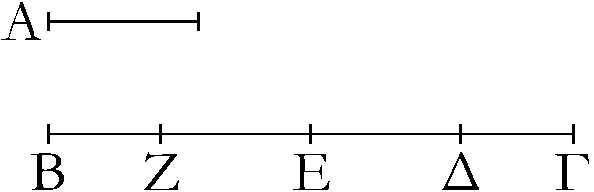
\includegraphics{Book10/fig018g.pdf}}

\gr{Τῶν γὰρ α\kern -.7pt  ὐτῶν κατασκευασθέντων τῶ| πρότερον ὁμοίωξ δείχομεν,
<ότι ἡ ΒΓ τῆξ Α μεῖζον δύναται τῶ| ἀπὸ τῆξ ΖΔ. δεικτέον
[ο>ῦν], <ότι ἀσύμμετρόξ ἐστιν ἡ ΒΓ τῆ| ΔΖ μ\kern -.7pt  ήκει. ἐπεὶ γὰρ
ἀσύμμετρόξ ἐστιν ἡ  ΒΔ τῆ| ΔΓ μ\kern -.5pt  ήκει, ἀσύμμετροξ >άρα ἐστὶ καὶ
ἡ ΒΓ τῆ| ΓΔ μ\kern -.3pt  ήκει. ἀλλὰ ἡ ΔΓ σύμμετρόξ ἐστι συναμφοτέραιξ
ταῖξ ΒΖ, ΔΓ; καὶ ἡ ΒΓ >άρα ἀσύμμετρόξ ἐστι συναμφοτέραιξ
ταῖξ ΒΖ, ΔΓ. <ώστε καὶ λοιπῆ| τῆ| ΖΔ ἀσύμμετρόξ  >έστιν ἡ ΒΓ
μ\kern -.7pt  ήκει. καὶ ἡ ΒΓ τῆξ Α μεῖζον δύναται τῶ| ἀπὸ τῆξ ΖΔ; ἡ ΒΓ
>άρα τῆξ Α μεῖζον δύναται τῶ| ἀπὸ ἀσυμμέτρου ἑαυτῆ|.}

\gr{Δυνάσθω δὴ πάλιν ἡ ΒΓ τῆξ Α μεῖζον τῶ| ἀπὸ ἀσυμμέτρ\-ου
ἑαυτῆ|, τῶ| δὲ τετάρτῳ τοῦ ἀπὸ τῆξ Α >ίσον παρὰ τὴν
ΒΓ παραβεβλήσθω ἐλλεῖπον ε>ίδει τετραγώνῳ, καὶ >έστω τὸ ὑπὸ τῶν
ΒΔ, ΔΓ. δεικτέον, <ότι ἀσύμμετρόξ ἐστιν ἡ ΒΔ τῆ| ΔΓ μ\kern -.7pt  ήκει.}

\gr{Τῶν γὰρ α\kern -.7pt  ὐτῶν κατασκευασθέντων ὁμοίωξ δείχομεν, <ότι
ἡ ΒΓ τῆξ Α μεῖζον δύναται τῶ| ἀπὸ τῆξ ΖΔ. ἀλλὰ ἡ ΒΓ
τῆξ Α μεῖζον δύναται τῶ| ἀπὸ ἀσυμμέτρου ἑαυτῆ|. ἀσύμμετροξ
>άρα ἐστὶν ἡ ΒΓ τῆ| ΖΔ μ\kern -.7pt  ήκει; <ώστε καὶ λοιπῆ| συναμφοτέρῳ
τῆ| ΒΖ, ΔΓ ἀσύμμετρόξ ἐστιν ἡ ΒΓ. ἀλλὰ συναμφότεροξ ἡ ΒΖ,
ΔΓ τῆ| ΔΓ σύμμετρόξ ἐστι μ\kern -.5pt  ήκει; καὶ ἡ ΒΓ >άρα τῆ| ΔΓ
ἀσύμμετρόξ ἐστι μ\kern -.3pt  ήκει; <ώστε καὶ διελόντι ἡ ΒΔ τῆ| ΔΓ
ἀσύμμετρόξ ἐστι μ\kern -.7pt  ήκει.}

\gr{Ἐὰν >άρα >ῶσι δύο εὐθεῖαι, καὶ τὰ ἑχῆξ.}}

\ParallelRText{
\begin{center}
{\large Proposition 18}$^\dag$
\end{center}

If there are two unequal straight-lines,
and a (rectangle) equal to the fourth part of the (square) on the
lesser, falling short by a square figure, is applied to the greater, and
divides it into (parts which are) incommensurable [in length], then
 the  square on the greater  will be  larger than the  (square on the) lesser  by the (square)
on (some straight-line) incommensurable  (in length) with the greater.
And if the square on the greater is larger than the (square on the) lesser  by the (square)
on (some straight-line) incommensurable  (in length) with the greater, and
a (rectangle) equal to the fourth (part) of the (square) on the lesser,
falling short by a square figure, is applied to the greater, then it divides it into (parts
which are) incommensurable [in length].

Let $A$ and $BC$ be two unequal straight-lines, of which (let) $BC$ (be) the
greater. And let a (rectangle) equal to the fourth [part] of the (square) on the
lesser, $A$, falling short by a
square figure, be applied to $BC$. And let it be the (rectangle contained) by $BDC$. And let $BD$ be incommensurable in length with
$DC$. I say that that the square on $BC$ is greater than the (square on) $A$ by the (square) on (some straight-line) incommensurable (in length) with ($BC$).

% Removed epsf size command
\centerline{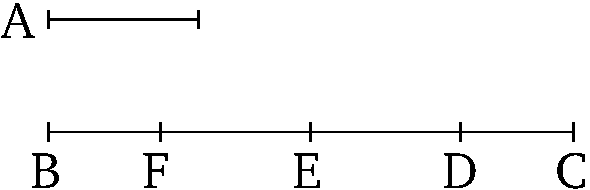
\includegraphics{Book10/fig018e.pdf}}

For, similarly, by the same construction as before, we can show that
the square on $BC$ is greater than the (square on) $A$ by the (square)
on $FD$. [Therefore] it must be shown that $BC$ is incommensurable
in length
with $DF$. For since $BD$ is incommensurable in length with $DC$, $BC$
is thus also incommensurable in length with $CD$ [Prop.~10.16]. But, $DC$ is commensurable (in length) with the sum of 
$BF$ and $DC$ [Prop.~10.6]. And, thus,
$BC$ is incommensurable (in  length) with the sum of $BF$ and $DC$ [Prop.~10.13]. Hence, $BC$ is also incommensurable in length with the remainder $FD$ [Prop.~10.16]. And the square on $BC$ is greater than the (square on) $A$ by the (square) on $FD$. Thus, the square on $BC$
is greater than the (square on) $A$ by the (square) on (some straight-line) incommensurable
(in length) 
with ($BC$).

So, again, let the square on $BC$ be greater than the (square on) $A$ by
the (square) on (some straight-line) incommensurable (in length) with ($BC$). And let a (rectangle) equal to the fourth [part] of the (square) on  $A$, falling short by a
square figure, be applied to $BC$.  And let it be the (rectangle contained) by $BD$ and $DC$. It must be shown that $BD$ is incommensurable in length with $DC$.

For, similarly, by the same construction, we can show that the square on $BC$ is greater than the (square) on $A$ by the (square) on $FD$. But,
the square on $BC$ is greater than the (square) on $A$ by the (square) on (some straight-line)
incommensurable (in length) with ($BC$). Thus, $BC$ is incommensurable in length with
$FD$. Hence, $BC$ is also incommensurable (in length) with the remaining sum of $BF$ and
$DC$ [Prop.~10.16]. But, the sum of
$BF$ and $DC$ is commensurable in length with $DC$ [Prop.~10.6]. Thus, $BC$ is also incommensurable
in length with $DC$ [Prop.~10.13]. Hence, via
separation, $BD$ is
also incommensurable in length with $DC$ [Prop.~10.16].

Thus,  if there are two \ldots straight-lines, and so on \ldots.}
\end{Parallel}
{\footnotesize\noindent$^\dag$ This proposition states that if $\alpha\,x-x^2=\beta^2/4$ (where $\alpha=BC$, $x=DC$,
and $\beta=A$) then $\alpha$ and $\sqrt{\alpha^2-\beta^2}$ are incommensurable when $\alpha-x$ are $x$ are incommensurable, and {\rm vice versa}.}

%%%%%%
% Prop 10.19
%%%%%%
\pdfbookmark[1]{Proposition 10.19}{pdf10.19}
\begin{Parallel}{}{} 
\ParallelLText{
\begin{center}
{\large \ggn{19}.}
\end{center}\vspace*{-7pt}

\gr{Τὸ ὑπὸ <ρητῶν μ\kern -.7pt  ήκει συμμέτρων  εὐθειῶν περιεχόμενον ὀρθογώνιον <ρητόν ἐστιν.}

\gr{Ὑπὸ γὰρ <ρητῶν μ\kern -.7pt  ήκει συμμέτρων εὐθειῶν τῶν
ΑΒ, ΒΓ ὀρθογώνιον περιεθέσθω τὸ ΑΓ; λέγω, <ότι <ρητόν ἐστι
τὸ ΑΓ.}\\

% Removed epsf size command
\centerline{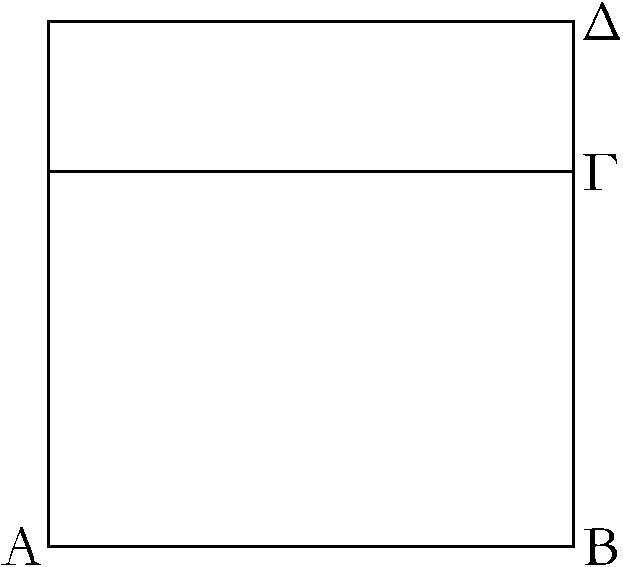
\includegraphics{Book10/fig019g.pdf}}

\gr{Ἀναγεγράφθω γὰρ ἀπὸ τῆξ ΑΒ τετράγωνον τὸ ΑΔ;
<ρητὸν >άρα ἐστὶ τὸ ΑΔ. καὶ ἐπεὶ σύμμετρόξ ἐστιν ἡ
ΑΒ τῆ| ΒΓ μ\kern -.7pt  ήκει, >ίση δέ ἐστιν ἡ ΑΒ τῆ| ΒΔ, σύμμετροξ
>άρα ἐστὶν ἡ ΒΔ τῆ| ΒΓ μ\kern -.7pt  ήκει. καί ἐστιν ὡξ ἡ ΒΔ πρὸξ τὴν
 ΒΓ, ο<ύτωξ τὸ ΔΑ πρὸξ τὸ ΑΓ. σύμμετρον
>άρα ἐστὶ τὸ ΔΑ τῶ| ΑΓ. <ρητὸν δὲ τὸ ΔΑ; <ρητὸν >άρα ἐστὶ
καὶ τὸ ΑΓ.}

\gr{Τὸ >άρα ὑπὸ <ρητῶν μ\kern -.7pt  ήκει συμμέτρων, καὶ τὰ ἑχῆξ.}}

\ParallelRText{
\begin{center}
{\large Proposition 19}
\end{center}

The rectangle contained by rational straight-lines
(which are) commensurable in length is rational.

For let the rectangle $AC$ be enclosed by the rational straight-lines
$AB$ and $BC$ (which are) commensurable in length. I say that
$AC$ is rational.

% Removed epsf size command
\centerline{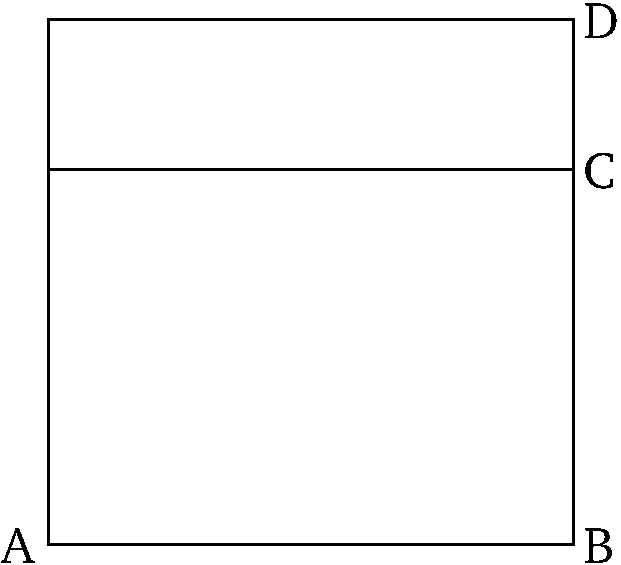
\includegraphics{Book10/fig019e.pdf}}

For let the square $AD$ be described on $AB$.  $AD$ is thus rational [Def.~10.4]. And since $AB$ is commensurable in length with $BC$, and $AB$ is equal to $BD$, $BD$ is thus
commensurable in  length with $BC$.  And as $BD$ is to
$BC$, so $DA$ (is) to $AC$ [Prop.~6.1]. Thus,
$DA$ is commensurable with $AC$ [Prop.~10.11]. 
And $DA$ (is) rational. Thus, $AC$ is also rational [Def.~10.4].
Thus,  the \ldots by rational straight-lines
\ldots commensurable, and so on \ldots.}
\end{Parallel}

%%%%%%
% Prop 10.20
%%%%%%
\pdfbookmark[1]{Proposition 10.20}{pdf10.20}
\begin{Parallel}{}{} 
\ParallelLText{
\begin{center}
{\large \ggn{20}.}
\end{center}\vspace*{-7pt}

\gr{Ἐὰν <ρητὸν παρὰ <ρητὴν παραβληθῆ|, πλάτοξ ποιεῖ <ρητὴν καὶ σύμμετρον τῆ|, παρ> <ὴν παράκειται, μ\kern -.7pt  ήκει.}\\~\\

% Removed epsf size command
\centerline{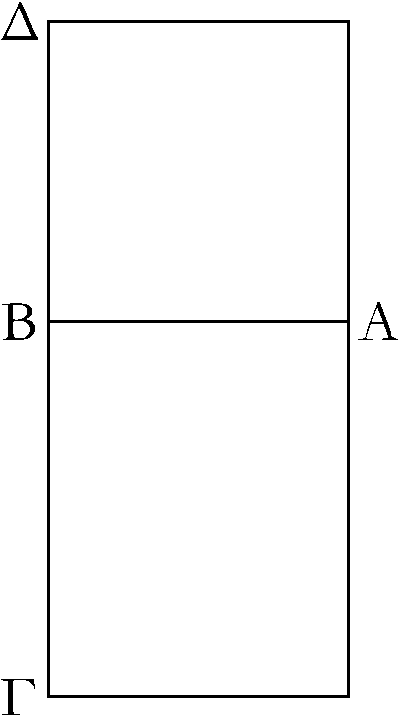
\includegraphics{Book10/fig020g.pdf}}

\gr{<Ρητὸν γὰρ τὸ ΑΓ παρὰ <ρητὴν τὴν ΑΒ παραβεβλήσθω πλάτοξ ποιοῦν τὴν ΒΓ; λέγω, <ότι
<ρητή ἐστιν ἡ ΒΓ καὶ σύμμετροξ τῆ| ΒΑ μ\kern -.7pt  ήκει.}

\gr{Ἀναγεγράφθω γὰρ ἀπὸ τῆξ ΑΒ τετράγωνον τὸ ΑΔ;
<ρητὸν >άρα ἐστὶ τὸ ΑΔ. <ρητὸν δὲ καὶ τὸ ΑΓ; σύμμετρον >άρα
ἐστὶ τὸ ΔΑ τῶ| ΑΓ. καί ἐστιν ὡξ τὸ ΔΑ πρὸξ τὸ ΑΓ, ο<ύτωξ
ἡ ΔΒ πρὸξ τὴν ΒΓ. σύμμετροξ >άρα ἐστὶ καὶ ἡ ΔΒ τῆ| ΒΓ;
>ίση δὲ ἡ ΔΒ τῆ| ΒΑ; σύμμετροξ >άρα καὶ ἡ
ΑΒ τῆ| ΒΓ.
<ρητὴ δέ ἐστιν ἡ ΑΒ; <ρητὴ >άρα ἐστὶ καὶ ἡ ΒΓ καὶ
σύμμετροξ τῆ| ΑΒ μ\kern -.7pt  ήκει.}

\gr{Ἐὰν >άρα <ρητὸν παρὰ <ρητὴν παραβληθῆ|, καὶ τὰ ἑχῆξ.}}

\ParallelRText{
\begin{center}
{\large Proposition 20}
\end{center}

If a rational (area) is applied to a rational (straight-line) then it produces as breadth  a (straight-line which is) rational, and commensurable in length
with the (straight-line) to which it is applied.

% Removed epsf size command
\centerline{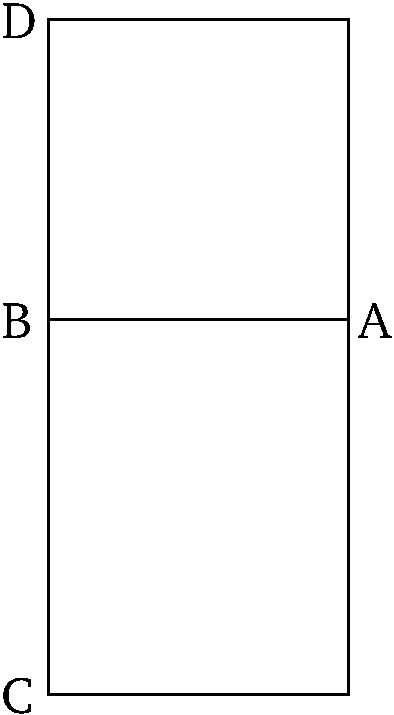
\includegraphics{Book10/fig020e.pdf}}

For let the rational (area) $AC$ be applied to the rational (straight-line) $AB$, producing the (straight-line) $BC$ as breadth. I say that
$BC$ is rational, and commensurable in length with $BA$.

For let the square $AD$ be described on $AB$. $AD$ is thus rational
[Def.~10.4]. And $AC$ (is) also rational. $DA$
is thus commensurable  with $AC$. And as $DA$ is to $AC$, so $DB$ (is)
to $BC$ [Prop.~6.1]. Thus, $DB$ is also
commensurable (in length) with $BC$ [Prop.~10.11]. And $DB$ (is) equal to $BA$. Thus, $AB$ (is)
also commensurable (in length) with $BC$. And $AB$ is rational. Thus, $BC$ is
also rational, and commensurable in length with $AB$ [Def.~10.3]. 

Thus, if  a rational (area) is applied to a rational (straight-line), and so
on \ldots.}
\end{Parallel}

%%%%%%
% Prop 10.21
%%%%%%
\pdfbookmark[1]{Proposition 10.21}{pdf10.21}
\begin{Parallel}{}{} 
\ParallelLText{
\begin{center}
{\large \ggn{21}.}
\end{center}\vspace*{-7pt}

\gr{Τὸ ὑπὸ <ρητῶν δυνάμει μόνον συμμέτρων εὐθειῶν περιεχόμενον
ὀρθογώνιον >άλογόν ἐστιν, καὶ ἡ δυναμένη α\kern -.7pt  ὐτὸ >άλογόξ ἐστιν,
καλείσθω δὲ μέση.}

% Removed epsf size command
\centerline{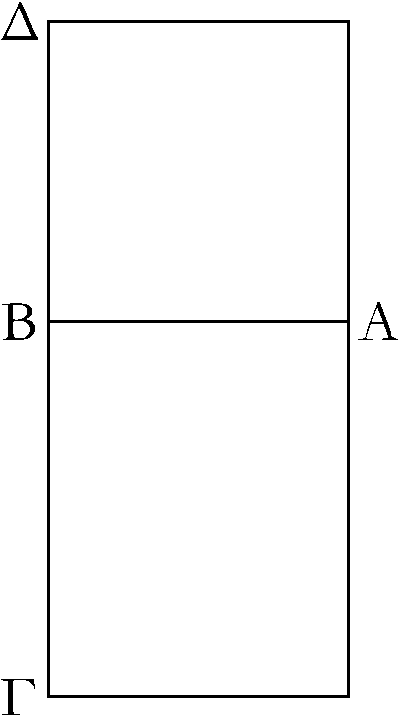
\includegraphics{Book10/fig020g.pdf}}

\gr{Ὑπὸ γὰρ <ρητῶν δυνάμει μόνον συμμέτρων εὐθειῶν τῶν
ΑΒ, ΒΓ ὀρθογώνιον περιεθέσθω τὸ ΑΓ; λέγω, <ότι >άλογόν ἐστι
τὸ ΑΓ, καὶ ἡ δυναμένη α\kern -.7pt  ὐτὸ >άλογόξ ἐστιν, καλείσθω δὲ μέση.}

\gr{Ἀναγεγράφθω γὰρ ἀπὸ τῆξ ΑΒ τετράγωνον τὸ ΑΔ; <ρητὸν >άρα
ἐστὶ τὸ ΑΔ. καὶ ἐπεὶ ἀσύμμετρόξ ἐστιν ἡ ΑΒ τῆ| ΒΓ μ\kern -.7pt  ήκει;
δυνάμει γὰρ μόνον ὑπόκεινται σύμμετροι; >ίση δὲ ἡ ΑΒ τῆ|
ΒΔ, ἀσύμμετροξ >άρα ἐστὶ καὶ ἡ ΔΒ τῆ| ΒΓ μ\kern -.7pt  ήκει. καί ἐστιν
ὡξ ἡ ΔΒ πρὸξ τὴν ΒΓ, ο<ύτωξ τὸ ΑΔ πρὸξ τὸ ΑΓ; ἀσύμμετρον
>άρα [ἐστὶ] τὸ ΔΑ τῶ| ΑΓ. <ρητὸν δὲ τὸ ΔΑ; >άλογον >άρα ἐστὶ
τὸ ΑΓ; <ώστε καὶ ἡ δυναμένη τὸ ΑΓ [τουτέστιν ἡ >ίσον α\kern -.5pt  ὐτῶ|
τετράγωνον δυναμένη] >άλογόξ ἐστιν, καλείσθω δε μέση; <όπερ >έδει
δεῖχαι.}}

\ParallelRText{
\begin{center}
{\large Proposition 21}
\end{center}

The rectangle contained by rational straight-lines (which are) commensurable in square only is irrational, and its square-root  is irrational---let it be called medial.$^\dag$

% Removed epsf size command
\centerline{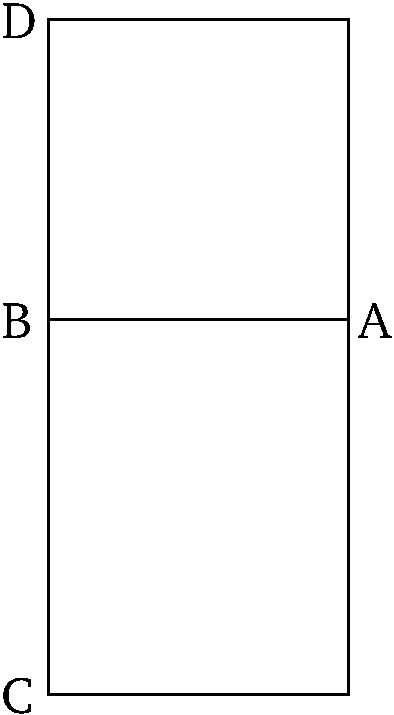
\includegraphics{Book10/fig020e.pdf}}

For let the rectangle $AC$ be contained by the rational straight-lines $AB$ and $BC$  (which are) commensurable in square only. I say that $AC$ is irrational, and
its square-root is irrational---let it be called
medial.

For let the square $AD$ be described on  $AB$. $AD$ is thus
rational [Def.~10.4]. And since $AB$ is incommensurable in length with $BC$. For they were assumed to be commensurable in square only. And $AB$ (is) equal to $BD$. $DB$ is thus
also incommensurable in length with $BC$. And as $DB$ is to $BC$, so
$AD$ (is) to $AC$ [Prop.~6.1]. Thus, $DA$ [is]
incommensurable with $AC$ [Prop.~10.11]. And $DA$ (is) rational. Thus, $AC$ is irrational [Def.~10.4]. Hence, its square-root [that is to say, the square-root of the square equal to it] is also irrational [Def.~10.4]---let it be called medial. (Which is) the
very thing it was required to show.}
\end{Parallel}
{\footnotesize\noindent$^\dag$ 
Thus, a medial straight-line has a length expressible as $k^{1/4}$.}

%%%%%%
% Prop 10.21a
%%%%%%
\begin{Parallel}{}{} 
\ParallelLText{
\begin{center}
{\large \gr{Λῆμμα}.}
\end{center}\vspace*{-7pt}

\gr{Ἐὰν >ῶσι δύο εὐθεῖαι, >έστιν ὡξ ἡ πρώτη πρὸξ τὴν
δευτέραν, ο<ύτωξ τὸ ἀπὸ τῆξ πρώτηξ πρὸξ τὸ ὑπὸ
τῶν δύο εὐθειῶν.}\\

% Removed epsf size command
\centerline{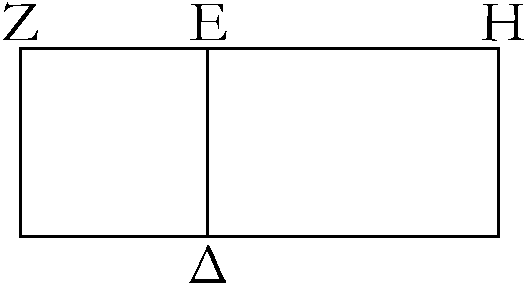
\includegraphics{Book10/fig021ag.pdf}}

\gr{>'Εστωσαν δύο εὐθεῖαι αἱ ΖΕ, ΕΗ. λέγω, <ότι ἐστὶν ὡξ ἡ ΖΕ
πρὸξ τὴν ΕΗ, ο<ύτωξ τὸ ἀπὸ τῆξ ΖΕ πρὸξ τὸ ὑπὸ τῶν
ΖΕ, ΕΗ.}

\gr{Ἀναγεγράφθω γὰρ ἀπὸ τῆξ ΖΕ τετράγωνον τὸ ΔΖ, καὶ συμπεπληρώσθω
τὸ ΗΔ. ἐπεὶ ο>ῦν ἐστιν ὡξ ἡ ΖΕ πρὸξ τὴν ΕΗ, ο<ύτωξ
τὸ ΖΔ πρὸξ τὸ ΔΗ, καί ἐστι τὸ μὲν ΖΔ τὸ ἀπὸ τῆξ ΖΕ, τὸ δὲ
ΔΗ τὸ ὑπὸ τῶν ΔΕ,  ΕΗ, τουτέστι τὸ ὑπὸ τῶν ΖΕ, ΕΗ, >έστιν
>άρα ὡξ ἡ ΖΕ πρὸξ τὴν ΕΗ, ο<ύτωξ τὸ ἀπὸ τῆξ ΖΕ πρὸξ
τὸ ὑπὸ τῶν ΖΕ, ΕΗ. ὁμοίωξ δὲ καὶ ὡξ τὸ ὑπὸ
τῶν ΗΕ, ΕΖ πρὸξ τὸ ἀπὸ τῆξ ΕΖ, τουτέστιν ὡξ τὸ ΗΔ πρὸξ τὸ ΖΔ,
ο<ύτωξ ἡ ΗΕ πρὸξ τὴν ΕΖ; <όπερ >έδει δεῖχαι.}}

\ParallelRText{
\begin{center}
{\large Lemma}
\end{center}

If there are two straight-lines then as the first is to the second, so the
(square) on the first (is) to the (rectangle contained) by the two straight-lines.

% Removed epsf size command
\centerline{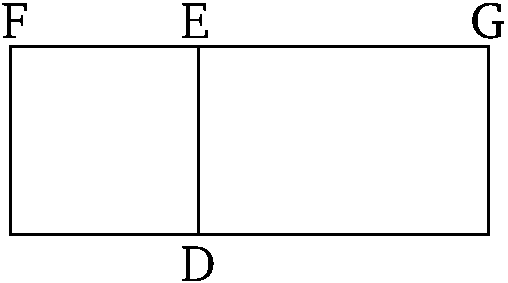
\includegraphics{Book10/fig021ae.pdf}}

Let $FE$ and $EG$ be two straight-lines. I say that as $FE$ is to $EG$,
so the (square) on $FE$ (is) to the (rectangle contained) by $FE$ and $EG$.

For let the square $DF$ be described on $FE$. And let $GD$ 
be completed. Therefore, since as $FE$ is to $EG$, so
$FD$ (is) to $DG$ [Prop.~6.1], and
$FD$ is the (square) on  $FE$, and $DG$ the (rectangle contained) by $DE$ and $EG$---that is to say,
the (rectangle contained) by $FE$ and $EG$---thus as $FE$ is to $EG$,
so the (square) on $FE$ (is) to the (rectangle contained) by $FE$ and $EG$. 
And also, similarly, as the (rectangle contained) by $GE$ and $EF$ is to the
(square on) $EF$---that is to say, as $GD$ (is) to $FD$---so $GE$
(is) to $EF$. (Which is) the very thing it was required to show.}
\end{Parallel}

%%%%%%
% Prop 10.22
%%%%%%
\pdfbookmark[1]{Proposition 10.22}{pdf10.22}
\begin{Parallel}{}{} 
\ParallelLText{
\begin{center}
{\large \ggn{22}.}
\end{center}\vspace*{-7pt}

\gr{Τὸ ἀπὸ μέσηξ παρὰ <ρητὴν παραβαλλόμενον πλάτοξ ποιεῖ <ρητὴν καὶ
ἀσύμμετρον τῆ|, παρ> <ὴν παράκειται, μ\kern -.7pt  ήκει.}

\gr{>'Εστω μέση μὲν ἡ Α, <ρητὴ δὲ ἡ ΓΒ, καὶ τῶ| ἀπὸ
τῆξ Α >ίσον παρὰ τὴν ΒΓ παραβεβλήσθω θωρίον ὀρθογώνιον τὸ ΒΔ
πλάτοξ ποιοῦν τὴν ΓΔ; λέγω, <ότι <ρητή ἐστιν ἡ ΓΔ καὶ
ἀσύμμετροξ τῆ| ΓΒ μ\kern -.7pt  ήκει.}\\~\\~\\

% Removed epsf size command
\centerline{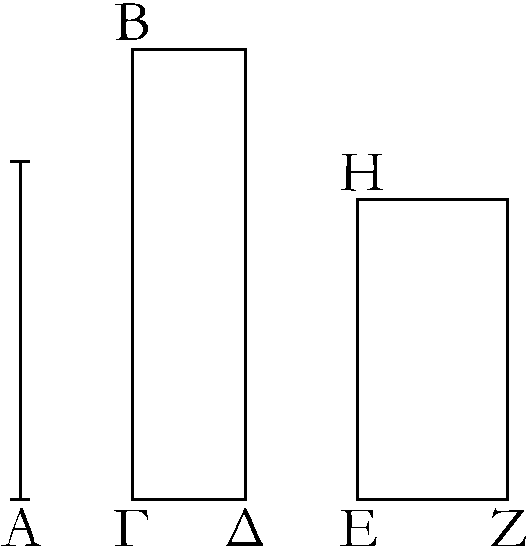
\includegraphics{Book10/fig022g.pdf}}

\gr{Ἐπεὶ γὰρ μέση ἐστὶν ἡ Α, δύναται θωρίον περιεχόμενον ὑπὸ
<ρητῶν δυνάμει μόνον συμμέτρων. δυνάσθω
τὸ ΗΖ. δύναται δὲ καὶ τὸ ΒΔ; >ίσον >άρα ἐστὶ τὸ ΒΔ τῶ| ΗΖ.
>έστι δὲ α\kern -.7pt  ὐτῶ| καὶ ἰσογώνιον; τῶν δὲ >ίσων τε καὶ ἰσογωνίων
παραλληλογράμμων ἀντιπεπόνθασιν αἱ πλευραὶ αἱ περὶ τὰξ
>ίσαξ  γωνίαξ; ἀνάλογον >άρα ἐστὶν ὡξ ἡ ΒΓ πρὸξ τὴν
ΕΗ, ο<ύτωξ ἡ ΕΖ πρὸξ τὴν ΓΔ. >έστιν >άρα καὶ ὡξ τὸ ἀπὸ
τῆξ ΒΓ πρὸξ τὸ ἀπὸ τῆξ ΕΗ, ο<ύτωξ τὸ ἀπὸ
 τῆξ ΕΖ πρὸξ τὸ ἀπὸ τῆξ ΓΔ. σύμμετρον δέ ἐστι τὸ ἀπὸ
τῆξ ΓΒ τῶ| ἀπὸ τῆξ ΕΗ; <ρητὴ γάρ ἐστιν ἑκατέρα α\kern -.7pt  ὐτῶν;
σύμμετρον >άρα ἐστὶ καὶ τὸ ἀπὸ τῆξ ΕΖ τῶ| ἀπὸ
τῆξ ΓΔ. <ρητὸν δέ ἐστι τὸ ἀπὸ τῆξ ΕΖ; <ρητὸν >άρα ἐστὶ
καὶ τὸ ἀπὸ τῆξ ΓΔ; <ρητὴ >άρα ἐστὶν ἡ ΓΔ. καὶ ἐπεὶ
ἀσύμμετρόξ ἐστιν ἡ ΕΖ τῆ| ΕΗ μ\kern -.5pt  ήκει; δυνάμει
γὰρ μόνον εἰσὶ σύμμετροι; ὡξ δὲ ἡ ΕΖ πρὸξ τὴν ΕΗ,
ο<ύτωξ τὸ ἀπὸ τῆξ ΕΖ πρὸξ τὸ ὑπὸ τῶν ΖΕ, ΕΗ, ἀσύμμετρον
>άρα [ἐστὶ] τὸ ἀπὸ τῆξ ΕΖ τῶ| ὑπὸ τῶν ΖΕ, ΕΗ. ἀλλὰ τῶ|
μὲν ἀπὸ τῆξ ΕΖ σύμμετρόν ἐστι τὸ ἀπὸ τῆξ ΓΔ; <ρηταὶ
γάρ εἰσι δυνάμει; τῶ| δὲ ὑπὸ τῶν ΖΕ, ΕΗ σύμμετρόν ἐστι
τὸ ὑπὸ τῶν ΔΓ, ΓΒ; >ίσα γάρ ἐστι τῶ| ἀπὸ τῆξ Α; ἀσύμμετρον
>άρα ἐστὶ καὶ τὸ ἀπὸ τῆξ ΓΔ τῶ| ὑπὸ τῶν ΔΓ, ΓΒ. ὡξ δὲ
τὸ ἀπὸ τῆξ ΓΔ πρὸξ τὸ ὑπὸ τῶν ΔΓ, ΓΒ, ο<ύτωξ
ἐστὶν ἡ ΔΓ πρὸξ τὴν ΓΒ; ἀσύμμετροξ >άρα ἐστὶν
ἡ ΔΓ τῆ| ΓΒ μ\kern -.3pt  ήκει. <ρητὴ >άρα ἐστὶν ἡ ΓΔ καὶ ἀσύμμετροξ
τῆ| ΓΒ μ\kern -.7pt  ήκει; <όπερ >έδει δεῖχαι.}}

\ParallelRText{
\begin{center}
{\large Proposition 22}
\end{center}

The square on a medial (straight-line), being
applied to a rational (straight-line), produces as breadth a (straight-line which
is) rational, and incommensurable in length with the (straight-line) to which it is applied.

Let $A$ be a medial (straight-line), and $CB$ a rational (straight-line),
and let the rectangular area $BD$, equal to the (square) on $A$, 
 be applied to $BC$, producing $CD$ as breadth. I say that
$CD$ is rational, and incommensurable in  length with $CB$.

% Removed epsf size command
\centerline{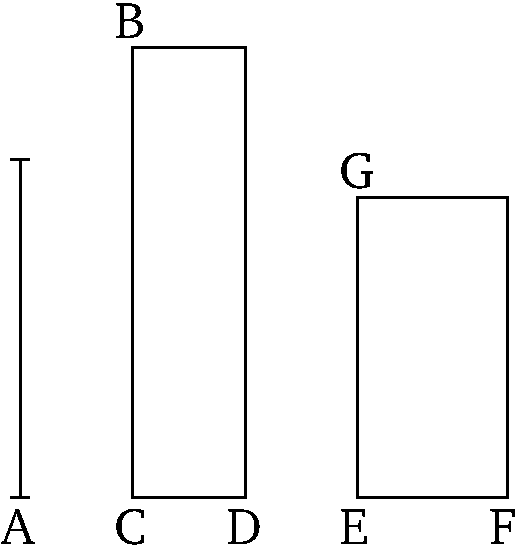
\includegraphics{Book10/fig022e.pdf}}

For since $A$ is medial, the square on it is equal to a (rectangular) area
contained by rational (straight-lines which are) commensurable in square
only [Prop.~10.21]. Let the square on ($A$) be equal
to $GF$. And the square on ($A$) is also equal to $BD$. Thus, $BD$
is equal to $GF$. And ($BD$) is also equiangular with ($GF$). And for equal and
equiangular parallelograms, the sides about the equal angles are
reciprocally proportional [Prop.~6.14]. 
Thus, proportionally,  as $BC$ is to $EG$, so $EF$ (is) to $CD$.
And, also, as the (square) on $BC$ is to the (square) on $EG$, so
the (square) on $EF$ (is) to the (square) on $CD$ [Prop.~6.22]. 
And the (square) on $CB$ is commensurable with the (square) on $EG$.
For they are each rational. Thus, the (square) on $EF$ is also commensurable
with the (square) on $CD$ [Prop.~10.11]. And
the (square) on $EF$ is rational. Thus, the (square) on $CD$ is also rational
[Def.~10.4]. Thus, $CD$ is rational.
And since $EF$ is incommensurable in length with
$EG$. For they are commensurable in square only. And as $EF$ (is) to $EG$,
so the (square) on $EF$ (is) to the (rectangle contained) by $FE$ and $EG$ 
[see previous lemma]. The (square) on $EF$ [is] thus incommensurable with the (rectangle contained) by $FE$ and $EG$ [Prop.~10.11]. But, the (square) on $CD$
is commensurable with the (square) on $EF$. For they are rational
in square.
And the (rectangle contained) by $DC$ and $CB$ is commensurable
with the (rectangle contained) by $FE$ and $EG$. For they are (both)
equal to the (square) on $A$. Thus, the (square) on $CD$ is also
incommensurable with the (rectangle contained) by $DC$ and $CB$
[Prop.~10.13]. And as the (square) on $CD$
(is) to the (rectangle contained) by $DC$ and $CB$, so $DC$ is to $CB$ [see
previous lemma]. Thus, $DC$ is incommensurable in length with $CB$
[Prop.~10.11]. Thus, $CD$ is rational, and
incommensurable in length with $CB$. (Which is) the very thing it was required to show.}
\end{Parallel}
{\footnotesize\noindent$^\dag$  Literally, ``rational''.\\}

%%%%%%%
% Prop 10.23
%%%%%%%
\pdfbookmark[1]{Proposition 10.23}{pdf10.23}
\begin{Parallel}{}{} 
\ParallelLText{
\begin{center}
{\large \ggn{23}.}
\end{center}\vspace*{-7pt}

\gr{Ἡ  τῆ| μέσῃ σύμμετροξ μέση ἐστίν.}

\gr{>'Εστω μέση ἡ Α, καὶ τῆ| Α σύμμετροξ >έστω ἡ Β; λέγω, <ότι καὶ
ἡ Β μέση ἐστίν.}

\gr{Ἐκκείσθω γὰρ <ρητὴ ἡ ΓΔ, καὶ τῶ| μὲν ἀπὸ τῆξ
Α >ίσον παρὰ τὴν ΓΔ παραβεβλήσθω θωρίον ὀρθογώνιον τὸ ΓΕ πλάτοξ
ποιοῦν τὴν ΕΔ; <ρητὴ >άρα ἐστὶν ἡ ΕΔ καὶ ἀσύμμετροξ τὴ|
ΓΔ μ\kern -.7pt  ήκει. τῶ| δὲ ἀπὸ τῆξ Β >ίσον παρὰ τὴν ΓΔ παραβεβλήσθω
θωρίον ὀρθογώνιον τὸ ΓΖ πλάτοξ ποιοῦν τὴν ΔΖ. ἐπεὶ ο>ῦν
σύμμετρόξ ἐστιν ἡ Α τῆ| Β, σύμμετρόν ἐστι καὶ τὸ ἀπὸ τῆξ Α τῶ|
ἀπὸ τῆξ Β. ἀλλὰ τῶ| μὲν ἀπὸ τῆξ Α >ίσον ἐστὶ τὸ ΕΓ, τῶ|
δὲ ἀπὸ τῆξ Β >ίσον ἐστὶ τὸ ΓΖ; σύμμετρον >άρα ἐστὶ τὸ ΕΓ τῶ| ΓΖ. καί ἐστιν ὡξ τὸ ΕΓ πρὸξ τὸ ΓΖ, ο<ύτωξ ἡ ΕΔ πρὸξ τὴν
ΔΖ; σύμμετροξ >άρα ἐστὶν ἡ ΕΔ τῆ| ΔΖ μ\kern -.7pt  ήκει. <ρητὴ δέ ἐστιν
ἡ ΕΔ καὶ ἀσύμμετροξ τῆ| ΔΓ μ\kern -.5pt  ήκει; <ρητὴ >άρα ἐστὶ καὶ ἡ ΔΖ
καὶ ἀσύμμετροξ τῆ| ΔΓ μ\kern -.3pt  ήκει; αἱ ΓΔ, ΔΖ >άρα <ρηταί εἰσι
δυνάμει μόνον σύμμετροι. ἡ δὲ τὸ ὑπὸ <ρητῶν δυνάμει
μόνον συμμέτρων δυναμένη μέση ἐστίν. ἡ >άρα τὸ ὑπὸ τῶν
ΓΔ, ΔΖ δυναμένη μέση ἐστίν; καὶ δύναται τὸ ὑπὸ τῶν ΓΔ, ΔΖ
ἡ Β; μέση >άρα ἐστὶν ἡ Β.}\\~\\~\\~\\~\\

% Removed epsf size command
\centerline{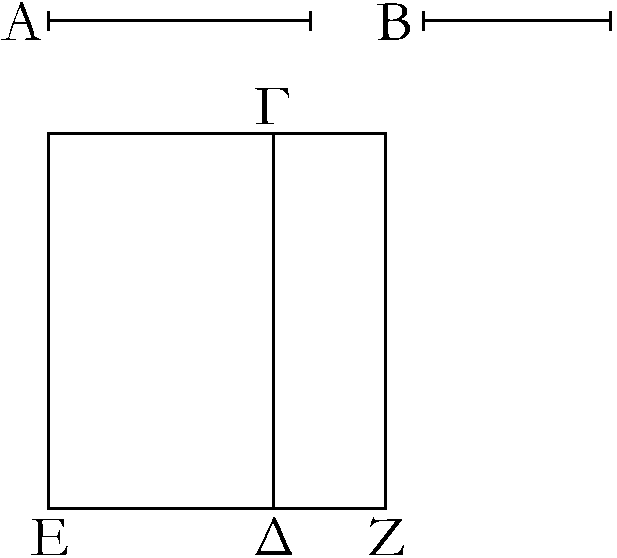
\includegraphics{Book10/fig023g.pdf}}

\begin{center}~\\
{\large \gr{Πόρισμα}.}
\end{center}\vspace*{-7pt}

\gr{Ἐκ δὴ τούτου φανερόν, <ότι τὸ τῶ| μέσῳ θωρίῳ σύμμετρ\-ον μέσον
ἐστίν.}}

\ParallelRText{
\begin{center}
{\large Proposition 23}
\end{center}

A (straight-line) commensurable with
a medial (straight-line) is medial.

Let $A$ be a medial (straight-line), and let $B$ be commensurable with $A$.
I say that $B$ is also a medial (staight-line).

Let the rational (straight-line) $CD$ be set out, and let the rectangular
area $CE$, equal to the (square) on $A$, be applied to $CD$,
producing $ED$ as width. $ED$ is thus rational, and incommensurable
in length with $CD$ [Prop.~10.22]. And
let the rectangular area $CF$, equal to the (square) on $B$, be
applied to $CD$, producing $DF$ as width.
Therefore, since $A$ is commensurable with $B$, the (square) on $A$
is also commensurable with the (square) on $B$.  But, $EC$ is equal
to the (square) on $A$, and $CF$ is equal to the (square) on $B$. Thus,
$EC$ is commensurable with $CF$. And as $EC$ is to $CF$, so $ED$ (is)
to $DF$ [Prop.~6.1]. Thus, $ED$ is commensurable
in  length with $DF$ [Prop.~10.11]. And $ED$
is rational, and incommensurable in length with $CD$.  $DF$ is thus
 also rational [Def.~10.3], and incommensurable in length with $DC$  [Prop.~10.13]. Thus,
 $CD$ and $DF$ are rational, and commensurable in square only.
 And the square-root of a (rectangle contained) by rational (straight-lines which are)
 commensurable in square only is medial [Prop.~10.21]. Thus, the square-root of the
 (rectangle contained) by $CD$ and $DF$ is medial.
 And the square on $B$ is equal to
 the (rectangle contained) by $CD$ and $DF$. Thus, $B$ is a medial (straight-line).
 
% Removed epsf size command
\centerline{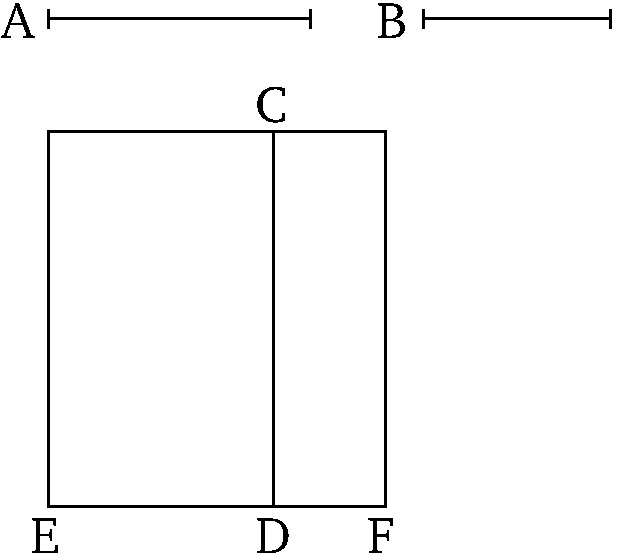
\includegraphics{Book10/fig023e.pdf}}
 
\begin{center}~\\
 {\large Corollary}
 \end{center}\vspace*{-7pt}
 
 And (it is) clear, from this, that an (area) commensurable with a medial 
 area$^\dag$ is medial.}
\end{Parallel}
{\footnotesize\noindent$^\dag$ A medial area is equal to the square on some medial straight-line. Hence, a medial area is expressible as $k^{1/2}$.}
 
%%%%%%
% Prop 10.24
%%%%%%
\pdfbookmark[1]{Proposition 10.24}{pdf10.24}
\begin{Parallel}{}{} 
\ParallelLText{
\begin{center}
{\large \ggn{24}.}
\end{center}\vspace*{-7pt}

\gr{Τὸ ὑπὸ μέσων μ\kern -.7pt  ήκει συμμέτρων εὐθειῶν  περιεχόμενον
ὀρθογώνιον μέσον
ἐστίν.}

\gr{Ὑπὸ γὰρ μέσων μ\kern -.7pt  ήκει συμμέτρων εὐθειῶν τῶν ΑΒ, ΒΓ
περιεθέσθω ὀρθογώνιον τὸ ΑΓ; λέγω, <ότι τὸ ΑΓ μέσον ἐστίν.}

\gr{Ἀναγεγράφθω γὰρ ἀπὸ τῆξ ΑΒ τετράγωνον τὸ ΑΔ; μέσον >άρα
ἐστὶ τὸ ΑΔ. καὶ ἐπεὶ σύμμετρόξ ἐστιν ἡ ΑΒ τῆ| ΒΓ
μ\kern -.7pt  ήκει, >ίση δὲ ἡ ΑΒ τῆ| ΒΔ, σύμμετροξ >άρα ἐστὶ καὶ ἡ ΔΒ τῆ|
ΒΓ μ\kern -.7pt  ήκει; <ώστε καὶ τὸ ΔΑ τῶ| ΑΓ σύμμετρόν ἐστιν. μέσον
δὲ τὸ ΔΑ; μέσον >άρα καὶ τὸ ΑΓ; <όπερ >έδει δεῖχαι.}\\~\\~\\

% Removed epsf size command
\centerline{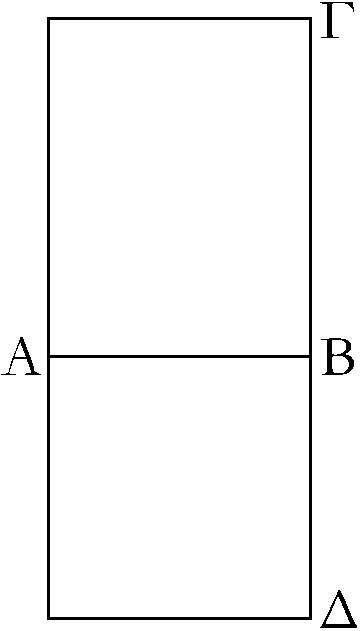
\includegraphics{Book10/fig024g.pdf}}
}

\ParallelRText{
\begin{center}
{\large Proposition 24}
\end{center}

A rectangle contained by medial straight-lines
(which are) commensurable in length is medial.

For let the rectangle $AC$ be contained by the medial straight-lines
$AB$ and $BC$ (which are) commensurable in length. I say that $AC$
is medial.

For let the square $AD$ be described on $AB$. $AD$ is thus medial [see previous footnote]. And since $AB$ is commensurable in length
with $BC$, and $AB$ (is) equal to $BD$, $DB$ is thus also commensurable
in length with $BC$. Hence, $DA$ is also commensurable with $AC$
[Props.~6.1, 10.11].
And $DA$ (is) medial. Thus, $AC$ (is) also medial [Prop.~10.23~corr.]. (Which is) the very thing it
was required to show.

% Removed epsf size command
\centerline{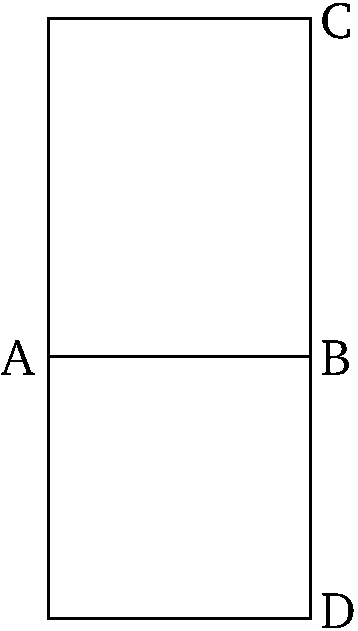
\includegraphics{Book10/fig024e.pdf}}}
\end{Parallel}

%%%%%%
% Prop 10.25
%%%%%%
\pdfbookmark[1]{Proposition 10.25}{pdf10.25}
\begin{Parallel}{}{} 
\ParallelLText{
\begin{center}
{\large \ggn{25}.}
\end{center}\vspace*{-7pt}

\gr{Τὸ ὑπὸ μέσων δυνάμει μόνον  συμμέτρων εὐθειῶν περιεχόμενον
ὀρθογώνιον >ήτοι <ρητὸν >ὴ μέσον ἐστίν.}

% Removed epsf size command
\centerline{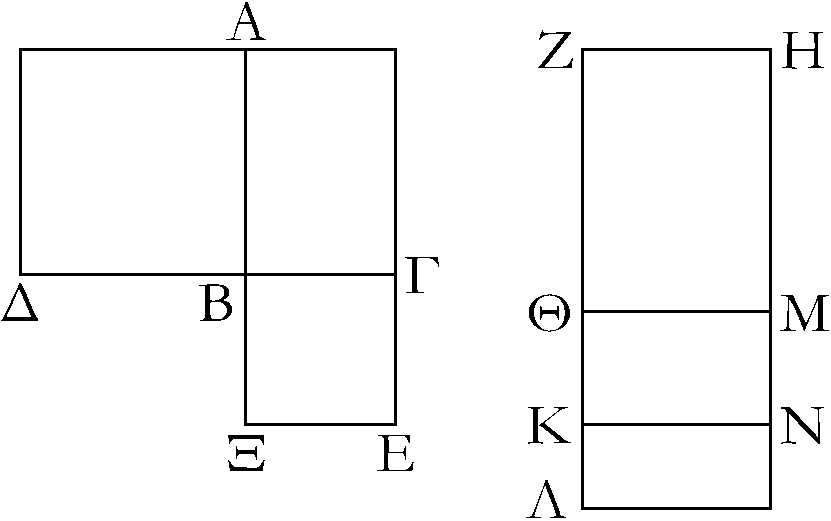
\includegraphics{Book10/fig025g.pdf}}

\gr{Ὑπὸ γὰρ μέσων δυνάμει μόνον συμμέτρων εὐθειῶν τῶν ΑΒ, ΒΓ
ὀρθογώνιον περιεθέσθω τὸ ΑΓ; λέγω, <ότι τὸ ΑΓ >ήτοι <ρητὸν
>ὴ μέσον ἐστίν.}

\gr{Ἀναγεγράφθω γὰρ ἀπὸ τῶν ΑΒ, ΒΓ τετράγωνα τὰ ΑΔ, ΒΕ; μέσον
>άρα ἐστὶν ἑκάτερον τῶν ΑΔ, ΒΕ. καὶ ἐκκείσθω <ρητὴ ἡ ΖΗ, καὶ
τῶ| μὲν ΑΔ >ίσον παρὰ τὴν ΖΗ παραβεβλήσθω ὀρθογώνιον παραλληλόγραμμον τὸ ΗΘ πλάτοξ ποιοῦν τὴν ΖΘ, τῶ| δὲ ΑΓ >ίσον
παρὰ τὴν ΘΜ παραβεβλήσθω ὀρθογώνιον παραλληλόγραμμον τὸ ΜΚ πλάτοξ
ποιοῦν τὴν ΘΚ, καὶ >έτι τῶ| ΒΕ >ίσον ὁμοίωξ παρὰ τὴν
ΚΝ παραβεβλήσθω τὸ ΝΛ πλάτοξ ποιοῦν τὴν ΚΛ; ἐπ> εὐθείαξ
>άρα εἰσὶν αἱ ΖΘ, ΘΚ, ΚΛ. ἐπεὶ ο>ῦν μέσον ἐστὶν ἑκάτερον
τῶν ΑΔ, ΒΕ, καί ἐστιν >ίσον τὸ μὲν ΑΔ τῶ| ΗΘ, τὸ δὲ ΒΕ τῶ|
ΝΛ, μέσον >άρα καὶ ἑκάτερον τῶν ΗΘ, ΝΛ. καὶ παρὰ <ρητὴν
τὴν ΖΗ παράκειται; <ρητὴ >άρα ἐστὶν ἑκατέρα τῶν ΖΘ, ΚΛ καὶ
ἀσύμμετροξ τῆ| ΖΗ μ\kern -.7pt  ήκει. καὶ ἐπεὶ σύμμετρόν ἐστι τὸ ΑΔ
τῶ| ΒΕ, σύμμετρον >άρα ἐστὶ καὶ τὸ ΗΘ τῶ| ΝΛ. καί ἐστιν
ὡξ τὸ ΗΘ πρὸξ τὸ ΝΛ, ο<ύτωξ ἡ ΖΘ πρὸξ τὴν ΚΛ;
σύμμετροξ >άρα ἐστὶν ἡ ΖΘ τῆ| ΚΛ μ\kern -.7pt  ήκει. αἱ ΖΘ, ΚΛ
>άρα <ρηταί εἰσι μ\kern -.5pt  ήκει σύμμετροι; <ρητὸν >άρα ἐστὶ τὸ ὑπὸ
τῶν ΖΘ, ΚΛ. καὶ ἐπεὶ >ίση ἐστὶν ἡ μὲν ΔΒ τῆ| ΒΑ, ἡ δὲ
ΧΒ τῆ| ΒΓ, >έστιν >άρα ὡξ ἡ ΔΒ πρὸξ τὴν ΒΓ, ο<ύτωξ ἡ ΑΒ
πρὸξ τὴν ΒΧ. ἀλλ> ὡξ μὲν ἡ ΔΒ πρὸξ τὴν ΒΓ, ο<ύτωξ
τὸ ΔΑ πρὸξ τὸ ΑΓ; ὡξ δὲ ἡ ΑΒ πρὸξ τὴν ΒΧ, ο<ύτωξ 
τὸ ΑΓ πρὸξ τὸ ΓΧ; >έστιν >άρα ὡξ τὸ ΔΑ πρὸξ τὸ ΑΓ, ο<ύτωξ
τὸ ΑΓ πρὸξ τὸ ΓΧ. >ίσον δέ ἐστι τὸ μὲν ΑΔ τῶ| ΗΘ, τὸ δὲ
ΑΓ τῶ| ΜΚ, τὸ δὲ ΓΧ τῶ| ΝΛ; >έστιν >άρα ὡξ τὸ ΗΘ πρὸξ τὸ ΜΚ,
ο<ύτωξ τὸ ΜΚ πρὸξ τὸ ΝΛ; >έστιν >άρα καὶ ὡξ
ἡ ΖΘ πρὸξ τὴν ΘΚ, ο<ύτωξ ἡ ΘΚ πρὸξ τὴν ΚΛ; τὸ >άρα ὑπὸ
τῶν ΖΘ, ΚΛ >ίσον ἐστὶ τῶ| ἀπὸ τῆξ ΘΚ. <ρητὸν δὲ τὸ ὑπὸ
τῶν ΖΘ, ΚΛ; <ρητὸν >άρα ἐστὶ καὶ τὸ ἀπὸ τῆξ ΘΚ; <ρητὴ >άρα ἐστὶν
ἡ ΘΚ. καὶ εἰ μὲν σύμμετρόξ ἐστι τῆ| ΖΗ μ\kern -.3pt  ήκει, <ρητόν ἐστι
τὸ ΘΝ; εἰ δὲ ἀσύμμετρόξ ἐστι τῆ| ΖΗ μ\kern -.7pt  ήκει, αἱ ΚΘ, ΘΜ <ρηταί
εἰσι δυνάμει μόνον σύμμετροι; μέσον >άρα τὸ ΘΝ. τὸ ΘΝ
>άρα >ήτοι <ρητὸν >ὴ μέσον ἐστίν. >ίσον δὲ τὸ ΘΝ τῶ| ΑΓ; τὸ
ΑΓ >άρα >ήτοι <ρητὸν >ὴ μέσον ἐστίν.}

\gr{Τὸ >άρα ὑπὸ μέσων δυνάμει μόνον συμμέτρων, καὶ τὰ εχῆξ.}}

\ParallelRText{
\begin{center}
{\large Proposition 25}
\end{center}

The rectangle contained by medial
straight-lines (which are) commensurable in square only is either
rational or medial.

% Removed epsf size command
\centerline{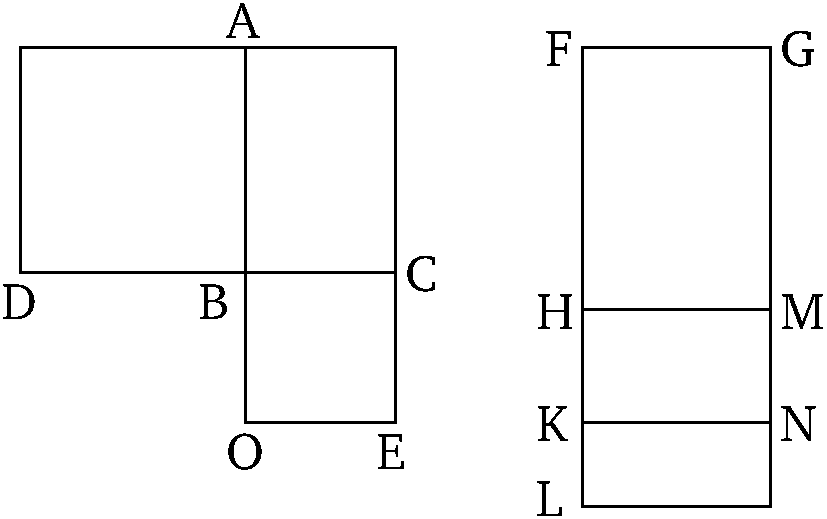
\includegraphics{Book10/fig025e.pdf}}

For let the rectangle $AC$ be contained by the medial straight-lines
$AB$ and $BC$ (which are) commensurable in square only. I say that
$AC$ is either rational or medial.

For let the squares $AD$ and $BE$ be described on (the straight-lines) $AB$ and
$BC$ (respectively). $AD$ and $BE$ are thus each medial. And let
the rational (straight-line) $FG$ be laid out. And let the rectangular parallelogram $GH$, equal to $AD$, be applied to $FG$, producing
$FH$ as breadth. And let the rectangular parallelogram $MK$, equal to $AC$, be applied to $HM$, producing $HK$ as breadth. And,
finally, let $NL$, equal to $BE$, have similarly been applied to $KN$,
producing $KL$ as breadth. Thus, $FH$, $HK$, and $KL$ are in
a straight-line.  Therefore, since $AD$ and $BE$ are each medial, and
$AD$ is equal to $GH$, and $BE$ to $NL$, $GH$ and $NL$ (are)
thus each also medial. And they are applied to the rational (straight-line)
$FG$. $FH$ and $KL$ are thus each rational, and incommensurable in length
with $FG$ [Prop.~10.22]. And since
$AD$ is commensurable with $BE$, $GH$ is thus also commensurable
with $NL$. And as $GH$ is to $NL$, so $FH$ (is) to $KL$ [Prop.~6.1]. Thus, $FH$ is commensurable
in length with $KL$ [Prop.~10.11]. Thus, 
$FH$ and $KL$ are rational (straight-lines which are) commensurable in length. Thus, the (rectangle contained) by $FH$ and $KL$ is rational
[Prop.~10.19]. And since $DB$ is equal to $BA$,
and $OB$ to $BC$, thus as $DB$ is to $BC$, so $AB$ (is) to $BO$.
But, as $DB$ (is) to $BC$, so $DA$ (is) to $AC$ [Props.~6.1]. 
And as $AB$ (is) to $BO$, so $AC$ (is)
to $CO$ [Prop.~6.1]. Thus, as $DA$ is to $AC$, so $AC$ (is)
to $CO$. And $AD$ is equal to $GH$,
and $AC$ to $MK$, and $CO$ to $NL$. Thus, as $GH$ is to $MK$,
so $MK$ (is) to $NL$. Thus, also, as $FH$ is to $HK$, so $HK$ (is) to
$KL$ [Props.~6.1, 5.11]. Thus, the (rectangle contained) by
$FH$ and $KL$ is equal to the (square) on $HK$ [Prop.~6.17]. And the (rectangle contained) by
$FH$ and $KL$ (is) rational. Thus, the (square) on $HK$ is also
rational. Thus, $HK$ is rational. And if it is commensurable in length with
$FG$ then $HN$ is rational [Prop.~10.19]. 
And if it is incommensurable in length with $FG$ then $KH$ and $HM$
are rational (straight-lines which are) commensurable in square only: thus,
$HN$ is medial [Prop.~10.21]. Thus, $HN$ is
either rational or medial. And $HN$ (is) equal to $AC$. Thus, $AC$
is either rational or medial.

Thus, the \ldots by medial
straight-lines (which are) commensurable in square only, and so on \ldots.}
\end{Parallel}

%%%%%%
% Prop 10.26
%%%%%%
\pdfbookmark[1]{Proposition 10.26}{pdf10.26}
\begin{Parallel}{}{} 
\ParallelLText{
\begin{center}
{\large \ggn{26}.}
\end{center}\vspace*{-7pt}

\gr{Μέσον μέσου οὐθ ὑπερέθει <ρητῶ|.}\\

% Removed epsf size command
\centerline{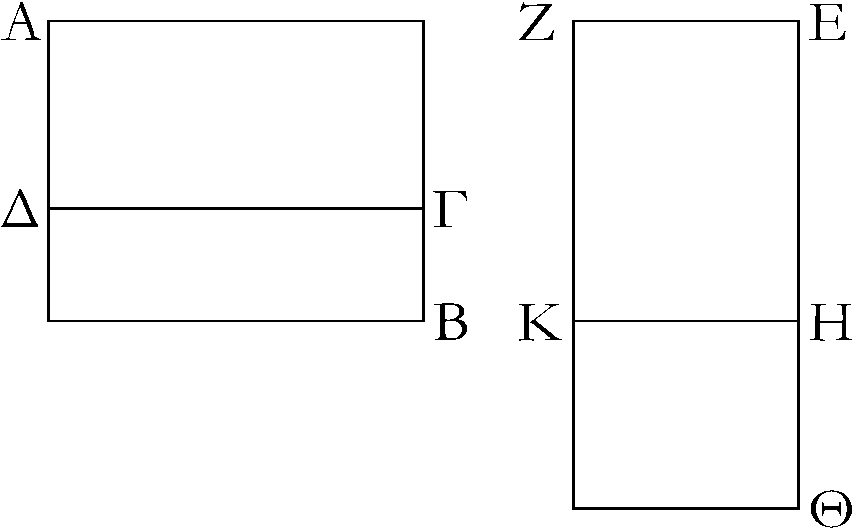
\includegraphics{Book10/fig026g.pdf}}

\gr{Εἰ γὰρ δυνατόν, μέσον τὸ ΑΒ μέσου τοῦ ΑΓ ὑπερεθέτω
<ρητῶ| τῶ| ΔΒ, καὶ ἐκκείσθω <ρητὴ ἡ ΕΖ, καὶ τῶ| ΑΒ
>ίσον παρὰ τὴν ΕΖ παραβεβλήσθω παραλληλόγραμμον ὀρθογώνιον
τὸ ΖΘ πλάτοξ ποιοῦν τὴν ΕΘ, τῶ| δὲ ΑΓ >ίσον ἀφῃρήσθω τὸ ΖΗ;
λοιπὸν >άρα τὸ ΒΔ λοιπῶ| τῶ| ΚΘ ἐστιν >ίσον. <ρητὸν δέ ἐστι
τὸ ΔΒ; <ρητὸν >άρα ἐστὶ καὶ τὸ ΚΘ. ἐπεὶ ο>ῦν μέσον ἐστὶν
ἑκάτερον τῶν ΑΒ, ΑΓ, καί ἐστι τὸ μὲν ΑΒ τῶ| ΖΘ >ίσον,
τὸ δὲ ΑΓ τῶ| ΖΗ, μέσον >άρα καὶ ἑκάτερον τῶν ΖΘ, ΖΗ. καὶ
παρὰ <ρητὴν τὴν ΕΖ παράκειται; <ρητὴ >άρα ἐστὶν ἑκατέρα
τῶν ΘΕ, ΕΗ καὶ ἀσύμμετροξ τῆ| ΕΖ μ\kern -.7pt  ήκει. καὶ ἐπεὶ <ρητόν
ἐστι τὸ ΔΒ καί ἐστιν >ίσον τῶ| ΚΘ, <ρητὸν >άρα ἐστὶ καὶ τὸ
ΚΘ. καὶ παρὰ <ρητὴν τὴν ΕΖ παράκειται; <ρητὴ >άρα ἐστὶν ἡ ΗΘ
καὶ σύμμετροξ τῆ| ΕΖ μ\kern -.7pt  ήκει. ἀλλά καὶ ἡ ΕΗ <ρητή ἐστι καὶ
ἀσύμμετροξ τῆ| ΕΖ μ\kern -.5pt  ήκει; ἀσύμμετροξ >άρα ἐστὶν ἡ ΕΗ
τῆ| ΗΘ μ\kern -.3pt  ήκει. καί ἐστιν ὡξ ἡ ΕΗ πρὸξ τὴν ΗΘ, ο<ύτωξ τὸ
ἀπὸ τῆξ ΕΗ πρὸξ τὸ ὑπὸ τῶν ΕΗ, ΗΘ; ἀσύμμετρον
>άρα ἐστὶ τὸ ἀπὸ τῆξ ΕΗ τῶ| ὑπὸ τῶν ΕΗ, ΗΘ. ἀλλὰ
τῶ| μὲν ἀπὸ τῆξ ΕΗ σύμμετρά ἐστι τὰ ἀπὸ τῶν ΕΗ, ΗΘ 
τετράγωνα; <ρητὰ γὰρ ἀμφότερα;
τῶ| δὲ ὑπὸ τῶν ΕΗ, ΗΘ σύμμετρόν ἐστι τὸ δὶξ ὑπὸ τῶν
ΕΗ, ΗΘ; διπλάσιον γάρ ἐστιν α\kern -.7pt  ὐτοῦ; ἀσύμμετρα >άρα ἐστὶ
τὰ ἀπὸ τῶν ΕΗ, ΗΘ τῶ| δὶξ ὑπὸ τῶν ΕΗ, ΗΘ; καὶ συναμφότερα >άρα
τά τε ἀπὸ τῶν ΕΗ, ΗΘ καὶ τὸ δὶξ ὑπὸ τῶν ΕΗ, ΗΘ, <όπερ
ἐστὶ τὸ ἀπὸ τῆξ ΕΘ, ἀσύμμετρόν ἐστι τοῖξ ἀπὸ τῶν ΕΗ, ΗΘ.
<ρητὰ δὲ τὰ ἀπὸ τῶν ΕΗ, ΗΘ; >άλογον >άρα τὸ ἀπὸ
τῆξ ΕΘ. >άλογοξ >άρα ἐστὶν ἡ ΕΘ. ἀλλὰ καὶ <ρηρή;
<όπερ ἐστὶν ἀδύνατον.}

\gr{Μέσον >άρα μέσου οὐθ ὑπερέθει <ρητῶ|; <όπερ >έδει
δεῖχαι.}}

\ParallelRText{
\begin{center}
{\large Proposition 26}
\end{center}

A medial (area) does not exceed a medial
(area) by a rational (area).$^\dag$

% Removed epsf size command
\centerline{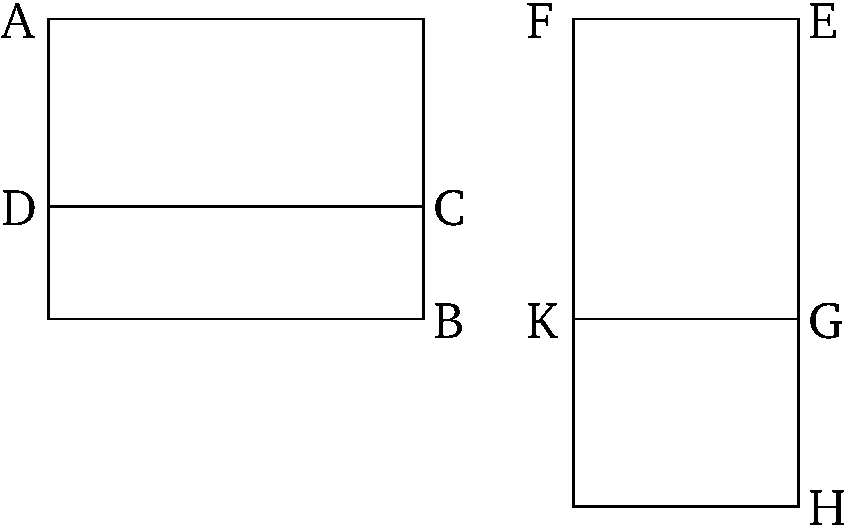
\includegraphics{Book10/fig026e.pdf}}

For, if possible, let the medial (area) $AB$ exceed the medial (area) $AC$
by the rational (area) $DB$. And let the rational (straight-line)
$EF$ be laid down. And let the rectangular parallelogram $FH$, equal to $AB$, be
applied to to $EF$, producing $EH$ as breadth. And let $FG$, equal to
$AC$, be cut off (from $FH$). Thus, the remainder $BD$
is equal to the remainder $KH$. And $DB$ is rational. Thus, $KH$
is also rational. Therefore, since $AB$ and $AC$ are each medial, and
$AB$ is equal to $FH$, and $AC$ to $FG$, $FH$ and $FG$ are thus each also medial. And they are applied to the rational (straight-line)
$EF$. Thus, $HE$ and $EG$ are each rational, and incommensurable
in length with $EF$ [Prop.~10.22]. 
And since $DB$ is rational, and is equal to $KH$, $KH$ is thus  also
rational. And ($KH$) is  applied to the rational (straight-line)
$EF$. $GH$ is thus rational, and commensurable in length with
$EF$ [Prop.~10.20]. But, $EG$ is also
rational, and incommensurable in length with $EF$. Thus, $EG$ is
incommensurable in length with $GH$ [Prop.~10.13]. And as $EG$ is to $GH$, so the
(square) on $EG$ (is) to the (rectangle contained) by $EG$ and
$GH$ [Prop.~10.13~lem.]. Thus, the (square)
on $EG$ is incommensurable with the (rectangle contained) by 
$EG$ and $GH$ [Prop.~10.11]. 
But, the (sum of the) squares on $EG$ and $GH$ is commensurable with
the (square) on $EG$. For ($EG$ and $GH$ are) both rational.
And twice the (rectangle contained) by $EG$ and $GH$ is commensurable
with the (rectangle contained) by $EG$ and $GH$ [Prop.~10.6]. For (the former) is double the latter.
Thus, the (sum of the squares) on $EG$ and $GH$ is incommensurable
with twice the (rectangle contained) by $EG$ and $GH$
[Prop.~10.13]. 
And thus the sum of the (squares) on $EG$ and $GH$ plus twice the (rectangle contained) by
$EG$ and $GH$, that is the (square) on $EH$ [Prop.~2.4], is incommensurable with the (sum
of the squares) on $EG$ and $GH$ [Prop.~10.16].
And the (sum of the squares) on $EG$ and $GH$ (is) rational. 
Thus, the (square) on $EH$ is irrational [Def.~10.4].
Thus, $EH$ is irrational  [Def.~10.4]. But,
(it is) also rational. The very thing is impossible.

Thus, a medial (area) does not exceed a medial
(area) by a rational (area). (Which is) the very thing it was required to show.}
\end{Parallel}
{\footnotesize\noindent$^\dag$ In other words, $\sqrt{k}-\sqrt{k'}\neq k''$.}

%%%%%%
% Prop 10.27
%%%%%%
\pdfbookmark[1]{Proposition 10.27}{pdf10.27}
\begin{Parallel}{}{} 
\ParallelLText{
\begin{center}
{\large \ggn{27}.}
\end{center}\vspace*{-7pt}

\gr{Μέσαξ εὑρεῖν δυνάμει μόνον συμμέτρουξ <ρητὸν περιεθούσαξ.}\\

% Removed epsf size command
\centerline{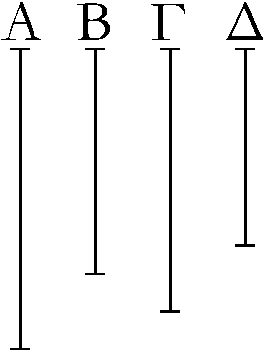
\includegraphics{Book10/fig027g.pdf}}

\gr{Ἐκκείσθωσαν δύο <ρηταὶ δυνάμει μόνον σύμμετροι αἱ
Α, Β, καὶ εἰλήφθω τῶν Α, Β μέση ἀνάλογον ἡ Γ, καὶ γεγονέτω
ὡξ ἡ Α πρὸξ τὴν Β, ο<ύτωξ ἡ Γ πρὸξ τὴν Δ.}

\gr{Καὶ ἐπεὶ αἱ Α, Β <ρηταί εἰσι δυνάμει μόνον σύμμετροι, τὸ
>άρα ὑπὸ τῶν Α, Β, τουτέστι τὸ ἀπὸ τῆξ Γ, μέσον ἐστίν.
μέση >άρα ἡ Γ. καὶ ἐπεί ἐστιν ὡξ ἡ Α πρὸξ τὴν Β,
[ο<ύτωξ] ἡ Γ πρὸξ τὴν Δ, αἱ δὲ Α, Β δυνάμει μόνον [εἰσὶ]
σύμμετροι, καὶ αἱ Γ, Δ >άρα δυνάμει μόνον εἰσὶ σύμμετροι. καί
ἐστι μέση ἡ Γ; μέση >άρα καὶ ἡ Δ. αἱ Γ, Δ >άρα μέσαι εἰσὶ
δυνάμει μόνον σύμμετροι. λέγω, <ότι καὶ <ρητὸν περιέθουσιν.
ἐπεὶ γάρ ἐστιν ὡξ ἡ Α πρὸξ τὴν Β, ο<ύτωξ ἡ Γ πρὸξ
τὴν Δ, ἐναλλὰχ >άρα ἐστὶν ὡξ ἡ Α πρὸξ τὴν Γ, ἡ Β
πρὸξ τὴν Δ. ἀλλ> ὡξ ἡ Α πρὸξ τὴν Γ, ἡ Γ πρὸξ τὴν Β; καὶ ὡξ
>άρα ἡ Γ πρὸξ τὴν Β, ο<ύτωξ ἡ Β πρὸξ τὴν Δ; τὸ >άρα
ὑπὸ τῶν Γ, Δ >ίσον ἐστὶ τῶ| ἀπὸ τῆξ Β. <ρητὸν δὲ τὸ
ἀπὸ τῆξ Β; <ρητὸν >άρα [ἐστὶ] καὶ τὸ ὑπὸ τῶν
Γ, Δ.}

\gr{Ε<ύρηνται >άρα μέσαι δυνάμει μόνον σύμμετροι <ρητὸν περιέθουσαι;
<όπερ >έδει δεῖχαι.}}

\ParallelRText{
\begin{center}
{\large Proposition 27}
\end{center}

To find (two) medial (straight-lines), containing a rational (area), (which are) commensurable in square only.

% Removed epsf size command
\centerline{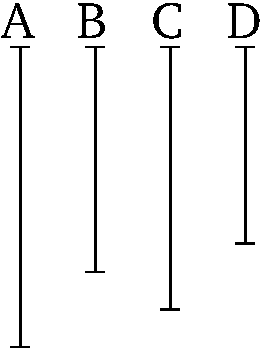
\includegraphics{Book10/fig027e.pdf}}

Let the two rational (straight-lines) $A$ and $B$, (which are) commensurable
in square only, be laid down. And let $C$---the mean proportional (straight-line) to
$A$ and $B$---be taken [Prop.~6.13]. 
And let it be contrived that as $A$ (is) to $B$, so $C$ (is) to $D$
[Prop.~6.12].

And since the rational (straight-lines) $A$ and $B$ are commensurable in square only,  the (rectangle contained) by $A$ and $B$---that is to
say, the (square) on $C$ [Prop.~6.17]---is thus medial
[Prop~10.21]. Thus, $C$ is medial
[Prop.~10.21]. And since as $A$ is to $B$, [so]
$C$ (is) to $D$, and $A$ and $B$ [are] commensurable in square only, 
$C$ and $D$ are thus also commensurable in square only [Prop.~10.11]. And $C$ is medial.
Thus, $D$ is also medial [Prop.~10.23]. 
Thus, $C$ and $D$ are medial (straight-lines which are) commensurable
in square only. I say that they also contain a rational (area).
For since as $A$ is to $B$, so $C$ (is) to $D$, thus, alternately,
as $A$ is to $C$, so $B$ (is) to $D$ [Prop.~5.16]. 
But, as $A$ (is) to $C$, (so) $C$ (is) to $B$. 
And thus as $C$ (is) to $B$, so $B$ (is) to $D$ [Prop.~5.11].
 Thus, the (rectangle contained) by $C$ and $D$ is equal to the (square) on $B$ [Prop.~6.17]. And the (square) on $B$ (is) rational. Thus, the (rectangle contained) by $C$ and $D$ [is] also rational.
 
Thus, (two) medial (straight-lines, $C$ and $D$), containing a rational (area), (which are) commensurable in square only, be found.$^\dag$ (Which is) the very thing it was required to show.}
\end{Parallel}
{\footnotesize\noindent$^\dag$ $C$ and $D$ have lengths $k^{1/4}$ and $k^{3/4}$ times that of $A$, respectively, where the length of $B$ is $k^{1/2}$ times that of $A$.}

%%%%%%
% Prop 10.28
%%%%%%
\pdfbookmark[1]{Proposition 10.28}{pdf10.28}
\begin{Parallel}{}{} 
\ParallelLText{
\begin{center}
{\large\ggn{28}.}
\end{center}\vspace*{-7pt}

\gr{Μέσαξ εὑρεῖν δυνάμει μόνον συμμέτρουξ μέσον πειριεθούσαξ.}

% Removed epsf size command
\centerline{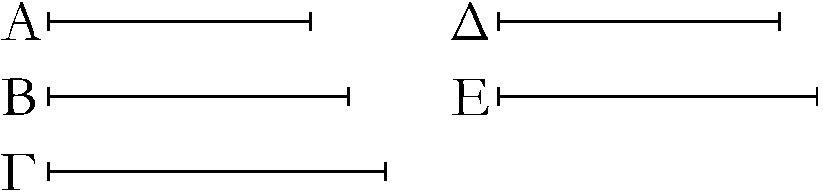
\includegraphics{Book10/fig028g.pdf}}

\gr{Ἐκκείσθωσαν [τρεῖξ] <ρηταὶ δυνάμει μόνον σύμμετροι αἱ Α, Β, Γ,
καὶ εἰλήφθω τῶν Α, Β μέση ἀνάλογον ἡ Δ, καὶ γεγονέτω ὡξ ἡ
Β πρὸξ τὴν Γ, ἡ Δ πρὸξ τὴν Ε.}

\gr{Ἐπεὶ αἱ Α, Β <ρηταί εἰσι δυνάμει μόνον σύμμετροι, τὸ >άρα
ὑπὸ τῶν Α, Β, τουτέστι τὸ ἀπὸ τῆξ Δ, μέσον ἐστὶν. μέση >άρα
ἡ Δ. καὶ ἐπεὶ αἱ Β, Γ δυνάμει μόνον εἰσὶ σύμμετροι, καί
ἐστιν ὡξ ἡ Β πρὸξ τὴν Γ,  ἡ Δ πρὸξ τὴν Ε, καὶ αἱ Δ, Ε >άρα
δυνάμει μόνον εἰσὶ σύμμετροι. μέση δὲ ἡ Δ; μέση >άρα καὶ
ἡ Ε; αἱ Δ, Ε >άρα μέσαι εἰσὶ δυνάμει μόνον σύμμετροι. λέγω
δή, <ότι καὶ μέσον περιέθουσιν. ἐπεὶ γάρ ἐστιν ὡξ ἡ Β
πρὸξ τὴν Γ, ἡ Δ πρὸξ τὴν Ε, ἐναλλὰχ >άρα ὡξ ἡ Β πρὸξ
τὴν Δ, ἡ Γ πρὸξ τὴν Ε. ὡξ δὲ ἡ Β πρὸξ τὴν Δ, ἡ Δ πρὸξ
τὴν Α; καὶ ὡξ <άρα ἡ Δ πρὸξ τὴν Α, ἡ Γ πρὸξ τὴν Ε;
τὸ >άρα ὑπὸ τῶν Α, Γ >ίσον ἐστὶ τῶ| ὑπὸ τῶν Δ, Ε.
μέσον δὲ τὸ ὑπὸ τῶν Α, Γ; μέσον >άρα καὶ τὸ ὑπὸ τῶν
Δ, Ε.}

\gr{Ἐ<ύρηνται >άρα μέσαι δυνάμει μόνον σύμμετροι μέσον περιέθουσαι;
<όπερ >έδει δεῖχαι.}}

\ParallelRText{
\begin{center}
{\large Proposition 28}
\end{center}

To find (two) medial (straight-lines),
containing a medial (area), (which are)
commensurable in square only.

% Removed epsf size command
\centerline{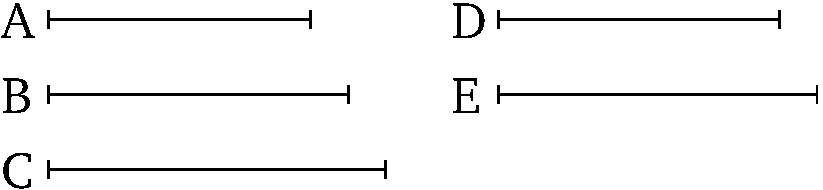
\includegraphics{Book10/fig028e.pdf}}

Let the [three] rational (straight-lines) $A$, $B$, and $C$, (which are)
commensurable in square only, be laid down. And let, $D$,  the mean proportional
(straight-line) to $A$ and $B$, be taken [Prop.~6.13]. And let it be contrived that as
$B$ (is) to $C$, (so) $D$ (is) to $E$ [Prop.~6.12].

Since the rational (straight-lines) $A$ and $B$ are commensurable in square only, the (rectangle contained) by $A$ and $B$---that is to say, the
(square) on $D$ [Prop.~6.17]---is medial
[Prop.~10.21]. Thus, $D$ (is) medial [Prop.~10.21]. And
since $B$ and $C$ are commensurable in square only, and as $B$ is to $C$, (so) $D$ (is) to $E$, $D$ and $E$ are thus commensurable in square
only [Prop.~10.11]. And $D$ (is) medial.
$E$ (is) thus also medial [Prop.~10.23].
Thus, $D$ and $E$ are medial (straight-lines which are) commensurable
in square only. So, I say that they also enclose a medial (area). For since
as $B$ is to $C$, (so) $D$ (is) to $E$, thus, alternately, as $B$ (is) to $D$,
(so) $C$ (is) to $E$ [Prop.~5.16]. And as
$B$ (is) to $D$, (so) $D$ (is) to $A$. And thus as $D$ (is) to $A$, (so)
$C$ (is) to $E$. Thus, the (rectangle contained) by $A$ and $C$ is equal
to the (rectangle contained) by $D$ and $E$ [Prop.~6.16]. And the (rectangle contained) by 
$A$ and $C$ is medial [Prop.~10.21]. Thus, the (rectangle contained) by $D$ and $E$ (is)
also medial.

Thus, (two) medial (straight-lines, $D$ and $E$), containing a medial (area),
(which are) commensurable in square only, be found. (Which is)
the very thing it was required to show.}
\end{Parallel}
{\footnotesize\noindent$^\dag$ $D$ and $E$ have lengths $k^{1/4}$ and $k'^{1/2}/k^{1/4}$ times that of $A$, respectively, where the lengths of $B$ and $C$ are
$k^{1/2}$ and $k'^{1/2}$ times that of $A$, respectively.}

%%%%%%
% Prop 10.28a
%%%%%%
\begin{Parallel}{}{} 
\ParallelLText{
\begin{center}{\large \gr{Λῆμμα \kern -.7pt {1}.}}
\end{center}\vspace*{-7pt}

\gr{Εὑρειν δύο τετραγώνουξ ἀριθμούξ, <ώστε καὶ τὸν συγκείμενον
ἐχ α\kern -.7pt  ὐτῶν ε>ῖναι τετράγωνον.}

% Removed epsf size command
\centerline{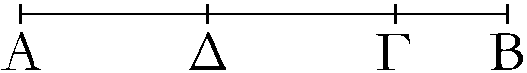
\includegraphics{Book10/fig028ag.pdf}}

\gr{Ἐκκείσθωσαν δύο ἀριθμοὶ οἱ ΑΒ, ΒΓ, >έστωσαν δὲ >ήτοι >άρτιοι
>ὴ περιττοί. καὶ ἐπεὶ, ἔαν τε ἀπὸ ἀρτίου >άρτιοξ ἀφαιρεθῆ|, ἔαν
τε ἀπὸ περισσοῦ περισσόξ, ὁ λοιπὸξ >άρτιόξ ἐστιν, ὁ λοιπὸξ
>άρα ὁ ΑΓ >άρτιόξ ἐστιν. τετμ\kern -.7pt  ήσθω ὁ ΑΓ δίθα κατὰ τὸ Δ. >έστωσαν
δὲ καὶ οἱ ΑΒ, ΒΓ >ήτοι <όμοιοι ἐπίπεδοι >ὴ τετράγωνοι,
ο<ὶ καὶ α\kern -.7pt  ὐτοὶ <όμοιοί εἰσιν ἐπίπεδοι;
 ὁ >άρα ἐκ τῶν
ΑΒ, ΒΓ μετὰ τοῦ ἀπὸ [τοῦ] ΓΔ τετραγώνου >ίσοξ ἐστὶ τῶ|
ἀπὸ τοῦ ΒΔ τετραγώνῳ. καί ἐστι τετράγωνοξ ὁ ἐκ
τῶν ΑΒ, ΒΓ, ἐπειδήπερ ἐδείθθη, <ότι, ἒαν δύο <όμοιοι
ἐπίπεδοι πολλαπλασιάσαντεξ ἀλλήλουξ ποιῶσι τινα, ὁ
γενόμενοξ τετράγωνόξ ἐστιν. ε<ύρηνται >άρα δύο τετράγωνοι ἀριθμοὶ
<ό τε ἐκ τῶν ΑΒ, ΒΓ καὶ ὁ ἀπὸ τοῦ ΓΔ, ο<ὶ συντεθέντεξ
ποιοῦσι τὸν ἀπὸ τοῦ ΒΔ τετράγωνον.}

\gr{Καὶ φανερόν, <ότι ε<ύρηνται πάλιν δύο τετράγωνοι
<ό τε ἀπὸ τοῦ ΒΔ καὶ ὁ ἀπὸ τοῦ ΓΔ, <ώστε τὴν ὑπεροθὴν
α\kern -.7pt  ὐτῶν τὸν ὑπὸ ΑΒ, ΒΓ ε>ῖναι τετράγωνον, <όταν
οἱ ΑΒ, ΒΓ <όμοιοι >ῶσιν ἐπίπεδοι. <όταν δὲ μ\kern -.7pt  ὴ >ῶσιν
<όμοιοι ἐπίπεδοι, ε<ύρηνται δύο τετράγωνοι <ό τε ἀπὸ
τοῦ ΒΔ καὶ ὁ ἀπὸ τοῦ ΔΓ, <ῶν ἡ ὑπεροθὴ ὁ ὑπὸ
τῶν ΑΒ, ΒΓ οὐκ >έστι τετράγωνοξ; <όπερ >έδει δεῖχαι.}}

\ParallelRText{
\begin{center}
{\large Lemma I}
\end{center}

To find two square numbers such that
the sum of them is also  square.

% Removed epsf size command
\centerline{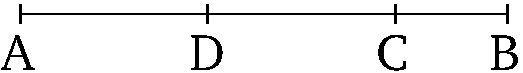
\includegraphics{Book10/fig028ae.pdf}}

Let the two numbers $AB$ and $BC$ be laid down. And let them
be either (both)  even or (both) odd. And since, if an even (number) is subtracted
from an even (number), or if an odd (number is subtracted) from an odd
(number), then the remainder is even [Props.~9.24, 9.26], the remainder $AC$ is thus even. Let
$AC$ be cut in half at $D$. And let $AB$ and $BC$ also be
either similar plane (numbers), or square (numbers)---which are themselves
also similar plane (numbers). Thus, the (number created) from (multiplying)  $AB$ and
$BC$, plus the square on $CD$, is equal to the square on $BD$ [Prop.~2.6].  And the (number created) from (multiplying) $AB$ and $BC$ is square---inasmuch as it was shown that
if two similar plane (numbers) make some (number) by multiplying
one another then the (number so) created is square [Prop.~9.1]. Thus, two square numbers be
found---(namely,) the (number created) from (multiplying) $AB$ and $BC$,
and the (square) on $CD$---which, (when) added (together),
make the square on $BD$.

And (it is) clear that two square (numbers) have again been found---(namely,) the (square) on $BD$, and the (square) on $CD$---such that their difference---(namely,) the (rectangle) contained by $AB$ and $BC$---is  square
whenever $AB$ and $BC$ are similar plane (numbers). But, when they are
not similar plane numbers, two square (numbers) be found---(namely,) the (square) on $BD$, and the (square) on $DC$---between which the difference---(namely,) the (rectangle) contained by $AB$ and $BC$---is
not  square. (Which is) the very thing it was required to show.}
\end{Parallel}

%%%%%%%
% Prop 10.28b
%%%%%%%
\begin{Parallel}{}{} 
\ParallelLText{
\begin{center}
{\large \gr{Λῆμμα \kern -.7pt {2}.}}
\end{center}\vspace*{-7pt}

\gr{Εὑρεῖν δύο τετραγώνουξ ἀριθμούξ, <ώστε τὸν ἐχ α\kern -.7pt  ὐτῶν συγκείμενον μ\kern -.7pt  ὴ ε>ῖναι τετράγωνον.}

% Removed epsf size command
\centerline{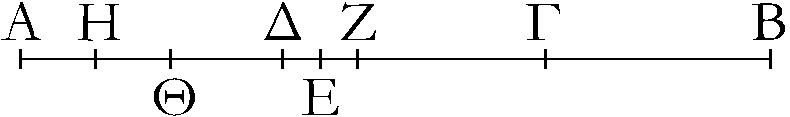
\includegraphics{Book10/fig028bg.pdf}}

\gr{>'Εστω γὰρ ὁ ἐκ τῶν ΑΒ, ΒΓ, ὡξ >έφαμεν, τετράγωνοξ, καὶ
>άρτιοξ ὁ ΓΑ, καὶ τετμ\kern -.7pt  ήσθω ὁ ΓΑ δίθα τῶ| Δ. φανερὸν δή,
<ότι ὁ ἐκ τῶν ΑΒ, ΒΓ τετράγωνοξ μετὰ τοῦ ἀπὸ [τοῦ]
ΓΔ τετραγώνου >ίσοξ ἐστὶ τῶ| ἀπὸ [τοῦ]
ΒΔ τετραγώνῳ. ἀφῃρήσθω μονὰξ ἡ ΔΕ; ὁ >άρα ἐκ τῶν ΑΒ, ΒΓ
μετὰ τοῦ ἀπὸ [τοῦ] ΓΕ ἐλάσσων ἐστὶ τοῦ ἀπὸ [τοῦ]
ΒΔ τετραγώνου. λέγω ο>ῦν, <ότι ὁ ἐκ τῶν ΑΒ, ΒΓ τετράγωνοξ μετὰ
τοῦ ἀπὸ [τοῦ] ΓΕ οὐκ >έσται τετράγωνοξ.}

\gr{Εἰ γὰρ >έσται τετράγωνοξ, >ήτοι >ίσοξ ἐστὶ τῶ| ἀπὸ [τοῦ]
ΒΕ >ὴ ἐλάσσων τοῦ ἀπὸ [τοῦ] ΒΕ, οὐκέτι δὲ καὶ μείζων, <ίνα
μ\kern -.7pt  ὴ τμ\kern -.7pt  ηθῆ| ἡ μονάξ. >έστω, εἰ δυνατόν, πρότερον ὁ ἐκ τῶν
ΑΒ, ΒΓ μετὰ τοῦ ἀπὸ ΓΕ >ίσοξ τῶ| ἀπὸ ΒΕ, καὶ >έστω τῆξ ΔΕ μονάδοξ διπλασίων ὁ ΗΑ. ἐπεὶ ο>ῦν <όλοξ ὁ ΑΓ <όλου
τοῦ ΓΔ ἐστι διπλασίων, <ῶν ὁ ΑΗ τοῦ ΔΕ ἐστι διπλασίων,
καὶ λοιπὸξ >άρα ὁ ΗΓ λοιποῦ τοῦ ΕΓ ἐστι διπλασίων;
δίθα >άρα τέτμ\kern -.5pt  ηται ὁ ΗΓ τῶ| Ε. ὁ >άρα ἐκ τῶν ΗΒ, ΒΓ
μετὰ τοῦ ἀπὸ ΓΕ >ίσοξ ἐστὶ τῶ| ἀπὸ ΒΕ τετραγώνῳ. 
ἀλλὰ καὶ
ὁ ἐκ τῶν ΑΒ, ΒΓ μετὰ τοῦ ἀπὸ ΓΕ >ίσοξ ὑπόκειται
τῶ| ἀπὸ [τοῦ] ΒΕ τετραγώνῳ; ὁ >άρα ἐκ τῶν ΗΒ, ΒΓ
μετὰ τοῦ ἀπὸ ΓΕ >ίσοξ ἐστὶ 
τῶ| ἐκ τῶν ΑΒ, ΒΓ μετὰ
τοῦ ἀπὸ ΓΕ. καὶ κοινοῦ ἀφαιρεθέντοξ τοῦ ἀπὸ ΓΕ συνάγεται
ὁ ΑΒ >ίσοξ τῶ| ΗΒ; <όπερ >άτοπον. οὐκ >άρα ὁ ἐκ τῶν ΑΒ, ΒΓ
μετὰ τοῦ ἀπὸ [τοῦ] ΓΕ >ίσοξ ἐστὶ τῶ| ἀπὸ ΒΕ. λέγω δή,
<ότι οὐδὲ ἐλάσσων τοῦ ἀπὸ ΒΕ. εἰ γὰρ δυνατόν, >έστω
τῶ| ἀπὸ ΒΖ >ίσοξ, καὶ τοῦ ΔΖ διπλασίων ὁ ΘΑ. καὶ συναθθήσεται
πάλιν διπλασίων ὁ ΘΓ τοῦ ΓΖ; <ώστε
καὶ τὸν ΓΘ δίθα τετμ\kern -.3pt  ῆσθαι κατὰ τὸ Ζ, καὶ διὰ τοῦτο
τὸν ἐκ τῶν ΘΒ, ΒΓ μετὰ τοῦ ἀπὸ ΖΓ >ίσον γίνεσθαι
τῶ| ἀπὸ ΒΖ. ὑπόκειται δὲ καὶ ὁ ἐκ τῶν ΑΒ, ΒΓ
μετὰ τοῦ ἀπὸ ΓΕ >ίσοξ τῶ| ἀπὸ ΒΖ. <ώστε καὶ ὁ ἐκ
τῶν ΘΒ, ΒΓ μετὰ τοῦ ἀπὸ ΓΖ >ίσοξ >έσται τῶ| ἐκ
τῶν ΑΒ, ΒΓ μετὰ τοῦ ἀπὸ ΓΕ; <όπερ >άτοπον. οὐκ
>άρα ὁ ἐκ τῶν ΑΒ, ΒΓ μετὰ τοῦ ἀπὸ ΓΕ >ίσοξ
ἐστὶ [τῶ|] ἐλάσσονι τοῦ ἀπὸ ΒΕ. ἐδείθθη δέ, <ότι οὐδὲ
[α\kern -.7pt  ὐτῶ|] τῶ| ἀπὸ ΒΕ. οὐκ >άρα ὁ ἐκ τῶν ΑΒ, ΒΓ μετὰ
τοῦ ἀπὸ ΓΕ τετράγωνόξ ἐστιν. <όπερ >έδει δεῖχαι.}}

\ParallelRText{
\begin{center}
{\large Lemma II}
\end{center}

To find two square numbers such that
the sum of them is not square.

% Removed epsf size command
\centerline{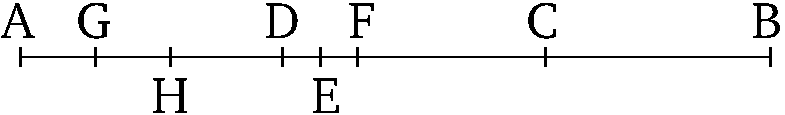
\includegraphics{Book10/fig028be.pdf}}

For let the (number created) from (multiplying) $AB$ and $BC$, as we said, be square.  And (let) $CA$ (be) even. And let $CA$ be
cut in half at $D$. So it is clear that the square (number created) from
(multiplying) $AB$ and $BC$, plus the square on $CD$, is equal to the
square on $BD$ [see previous lemma]. Let the unit $DE$ be subtracted (from $BD$).
Thus, the (number created) from (multiplying) $AB$ and $BC$, plus
the (square) on $CE$, is less than the square on $BD$. I say, therefore,
that the square (number created) from (multiplying) $AB$ and $BC$, plus the
(square) on $CE$, is not square.

For if it is square, it is either equal to the (square) on $BE$, or
less than the (square) on $BE$, but cannot    any more be greater  (than the square on $BE$), lest the unit be divided. First of all, if possible, let the
(number created) from (multiplying) $AB$ and $BC$, plus the (square) on
$CE$, be equal to the (square) on $BE$. And let $GA$ be double the unit
$DE$. Therefore, since the whole of $AC$ is double the whole
of $CD$, of which $AG$ is double $DE$, the remainder $GC$
is thus double the remainder $EC$. Thus, $GC$ has been cut in half at $E$.
Thus, the (number created) from (multiplying) $GB$ and $BC$,
plus the (square) on $CE$, is equal to the square on $BE$ [Prop.~2.6]. But, the (number created) from (multiplying) $AB$ and $BC$, plus the (square) on $CE$, was also assumed
 (to be) equal to the square on $BE$. Thus, the (number created) from
 (multiplying) $GB$ and $BC$, plus the (square) on $CE$, is equal to
 the (number created) from (multiplying)  $AB$ and $BC$, plus the
 (square) on $CE$. And subtracting the (square) on $CE$ from both, $AB$ is  inferred (to be) equal to $GB$. The very thing is absurd. Thus, the (number created) from (multiplying) $AB$ and $BC$, plus the (square) on
$CE$, is not equal to the (square) on $BE$. So I say that (it is) not
less than the (square) on $BE$ either. For, if possible, let it be equal to
the (square) on $BF$. And (let) $HA$ (be) double $DF$. And it
can again be inferred that $HC$ (is) double $CF$. Hence, $CH$ has
also been cut in half at $F$. And, on account of this, the (number created)
from (multiplying) $HB$ and $BC$, plus the (square) on $FC$, becomes
equal to the (square) on $BF$ [Prop.~2.6]. 
And the (number created) from (multiplying) $AB$ and $BC$, plus the
(square) on $CE$, was also
assumed (to be) equal to the (square) on $BF$.
Hence,
the (number created) from (multiplying) $HB$ and $BC$, plus the
(square) on $CF$, will also be equal to the
(number created) from (multiplying) $AB$ and $BC$, plus the (square) on $CE$. The very thing is
absurd. Thus, the (number created) from (multiplying) $AB$ and $BC$,
plus the (square) on $CE$, is not equal to less than the
(square) on $BE$. And it was shown that  (is it) not equal to the (square)
on $BE$ either. Thus, the (number created) from (multiplying)
$AB$ and $BC$, plus the  square on $CE$, is not square. (Which is)
the very thing it was required to show.}
\end{Parallel}

%%%%%%
% Prop 10.29
%%%%%%
\pdfbookmark[1]{Proposition 10.29}{pdf10.29}
\begin{Parallel}{}{} 
\ParallelLText{
\begin{center}
{\large \ggn{29}.}
\end{center}\vspace*{-7pt}

\gr{Εὑρεῖν δύο <ρητὰξ δυνάμει μόνον συμμέτρουξ, <ώστε τὴν μείζονα
τῆξ ἐλάσσονοξ μεῖζον δύνασθαι τῶ| ἀπὸ συμμέτρου ἑαυτῆ|
μ\kern -.7pt  ήκει.}\\~\\

% Removed epsf size command
\centerline{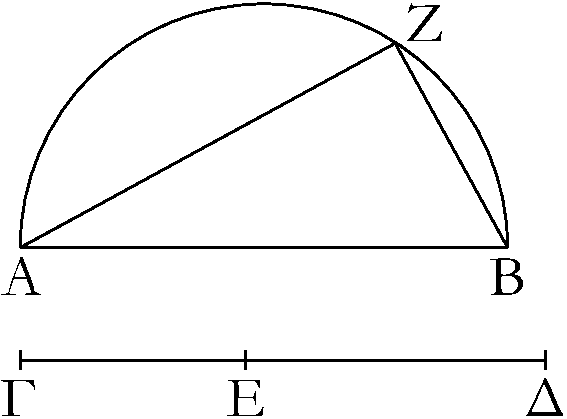
\includegraphics{Book10/fig029g.pdf}}

\gr{Ἐκκείσθω γάρ τιξ <ρητὴ ἡ ΑΒ καὶ δύο τετράγωνοι ἀριθμοὶ
οἱ ΓΔ, ΔΕ, <ώστε τὴν ὑπεροθὴν α\kern -.7pt  ὐτῶν τὸν ΓΕ μ\kern -.7pt  ὴ ε>ῖναι
τετράγωνον, καὶ γεγράφθω ἐπὶ τῆξ ΑΒ ἡμικύκλιον τὸ ΑΖΒ,
καὶ πεποιήσθω ὡξ ὁ ΔΓ πρὸξ τὸν ΓΕ, ο<ύτωξ τὸ ἀπὸ τῆξ ΒΑ
τετράγωνον πρὸξ τὸ ἀπὸ τῆξ ΑΖ τετράγωνον, καὶ ἐπεζεύθθω ἡ ΖΒ.}

\gr{Ἐπεὶ [ο>ῦν] ἐστιν ὡξ τὸ ἀπὸ τῆξ ΒΑ πρὸξ τὸ ἀπὸ τῆξ ΑΖ,
ο<ύτωξ ὁ ΔΓ πρὸξ τὸν ΓΕ, τὸ ἀπὸ τῆξ ΒΑ >άρα πρὸξ τὸ
ἀπὸ τῆξ ΑΖ λόγον >έθει, <όν ἀριθμὸξ ὁ ΔΓ πρὸξ ἀριθμὸν
τὸν ΓΕ; σύμμετρον >άρα ἐστὶ τὸ ἀπὸ τῆξ ΒΑ τῶ| ἀπὸ τῆξ
ΑΖ. <ρητὸν δὲ τὸ ἀπὸ τῆξ ΑΒ; <ρητὸν >άρα καὶ τὸ ἀπὸ
τῆξ ΑΖ; <ρητὴ >άρα καὶ ἡ ΑΖ. καὶ ἐπεὶ ὁ ΔΓ πρὸξ τὸν ΓΕ
λόγον οὐκ >έθει, <ὸν τετράγωνοξ ἀριθμὸξ πρὸξ τετράγωνον
ἀριθμόν,  οὐδὲ τὸ ἀπὸ τῆξ ΒΑ >άρα πρὸξ τὸ ἀπὸ τῆξ
ΑΖ λόγον >έθει, <ὸν τετράγωνοξ ἀριθμὸξ πρὸξ τετράγωνον
ἀριθμόν; ἀσύμμετροξ >άρα ἐστὶν ἡ ΑΒ τῆ| ΑΖ μ\kern -.7pt  ήκει; αἱ
ΒΑ, ΑΖ >άρα <ρηταί εἰσι δυνάμει μόνον σύμμετροι. καὶ ἐπεί
[ἐστιν] ὡξ ὁ ΔΓ πρὸξ τὸν ΓΕ, ο<ύτωξ τὸ ἀπὸ τῆξ ΒΑ πρὸξ
τὸ ἀπὸ τῆξ ΑΖ, ἀναστρέψαντι >άρα ὡξ ὁ ΓΔ πρὸξ τὸν
ΔΕ, ο<ύτωξ τὸ ἀπὸ τῆξ ΑΒ πρὸξ τὸ ἀπὸ τῆξ ΒΖ. ὁ δὲ
ΓΔ πρὸξ τὸν ΔΕ λόγον >έθει, <ὸν τετράγωνοξ ἀριθμὸξ
πρὸξ τετράγωνον ἀριθμόν; καὶ τὸ ἀπὸ τῆξ ΑΒ >άρα πρὸξ τὸ
ἀπὸ τῆξ ΒΖ λόγον >έθει, <ὸν τετράγωνοξ ἀριθμὸξ πρὸξ τετράγωνον
ἀριθμόν;
σύμμετροξ >άρα ἐστὶν ἡ ΑΒ
τῆ| ΒΖ μ\kern -.7pt  ήκει. καί ἐστι τὸ ἀπὸ τῆξ ΑΒ >ίσον τοῖξ ἀπὸ τῶν ΑΖ, ΖΒ; ἡ ΑΒ >άρα τῆξ ΑΖ μεῖζον δύναται τῆ|
ΒΖ συμμέτρῳ ἑαυτῆ|.}

\gr{Ε<ύρηνται >άρα δύο <ρηταὶ δυνάμει μόνον σύμμετροι αἱ ΒΑ, ΑΖ,
<ώστε τὴν μεῖζονα τὴν ΑΒ τῆξ ἐλάσσονοξ τῆξ ΑΖ μεῖζον δύνασθαι
τῶ| ἀπὸ τῆξ ΒΖ συμμέτρου ἑαυτῆ| μ\kern -.7pt  ήκει; <όπερ >έδει
δεῖχαι.}}

\ParallelRText{
\begin{center}
{\large Proposition 29}
\end{center}

To  find two rational (straight-lines which are)
commensurable in square only, such that the square on the greater is larger
than the (square on the) lesser by the (square) on (some straight-line which is) commensurable in length with the greater.

% Removed epsf size command
\centerline{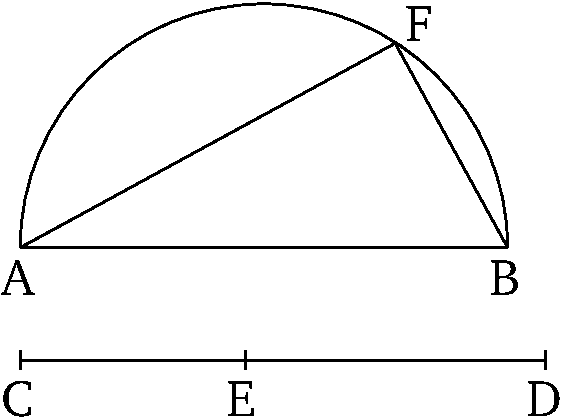
\includegraphics{Book10/fig029e.pdf}}

For let some rational (straight-line) $AB$ be laid down, and two
square numbers, $CD$ and $DE$, such that the difference between them, $CE$, is not square [Prop.~10.28 lem.~I]. 
And let the semi-circle $AFB$ be drawn on $AB$. And let
it be contrived that as $DC$ (is) to $CE$, so the square on $BA$
(is) to the square on $AF$ [Prop.~10.6~corr.].
And let $FB$ be joined.

\mbox{[}Therefore,] since as the (square) on $BA$ is to the (square) on $AF$,
so $DC$ (is) to $CE$, the (square) on $BA$ thus has to the (square)
on $AF$ the ratio which the number $DC$ (has) to the number $CE$.
Thus, the (square) on $BA$ is commensurable with the (square) on $AF$
[Prop.~10.6]. And the (square) on $AB$ (is)
rational [Def.~10.4]. Thus, the (square) on $AF$
(is) also rational. Thus, $AF$ (is) also rational. 
And since $DC$ does not have to $CE$ the ratio which
(some) square number (has) to (some) square number,  the (square)
on $BA$ thus does not have to the (square) on $AF$ the ratio which (some)
square number has to (some) square number either. Thus, $AB$ is incommensurable in length with $AF$ [Prop.~10.9].
Thus, the rational (straight-lines) $BA$
and $AF$ are commensurable in square only. And since as $DC$ [is] to $CE$, so the
(square) on $BA$ (is) to the (square) on $AF$, thus, via conversion,
as $CD$ (is) to $DE$, so the (square) on $AB$ (is) to the (square) on
$BF$ [Props.~5.19~corr., 3.31, 1.47]. And $CD$
has to $DE$ the ratio which (some) square number (has) to (some)
square number. Thus, the (square) on $AB$ also has to the (square) on
$BF$ the ratio which (some) square number has to (some) square number.
$AB$ is thus commensurable in length with $BF$ [Prop.~10.9]. And the (square) on $AB$
is equal to the (sum of the squares) on $AF$ and $FB$ [Prop.~1.47]. Thus, the
square on $AB$ is greater than (the square on) $AF$ by (the square on)
$BF$, (which is) commensurable (in length) with ($AB$).

Thus, two rational (straight-lines), $BA$ and $AF$, commensurable in square only, be found such that the square on the greater, $AB$, is larger
than (the square on) the lesser, $AF$, by the (square) on $BF$, (which is)
commensurable in length with ($AB$).$^\dag$ (Which is) the very thing it
was required to show.}
\end{Parallel}
{\footnotesize\noindent$^\dag$ $BA$ and $AF$
have lengths $1$ and $\sqrt{1-k^2}$ times that of $AB$, respectively, where $k=\sqrt{DE/CD}$.}

%%%%%%
% Prop 10.30
%%%%%%
\pdfbookmark[1]{Proposition 10.30}{pdf10.30}
\begin{Parallel}{}{} 
\ParallelLText{
\begin{center}
{\large \ggn{30}.}
\end{center}\vspace*{-7pt}

\gr{Εὑρεῖν δύο <ρητὰξ δυνάμει μόνον συμμέτρουξ, <ώστε τὴν
μείζονα τῆξ ἐλάσσονοξ μεῖζον δύνασθαι τῶ| ἀπὸ ἀσυμμέτρου
ἑαυτῆ| μ\kern -.7pt  ήκει.}\\~\\

% Removed epsf size command
\centerline{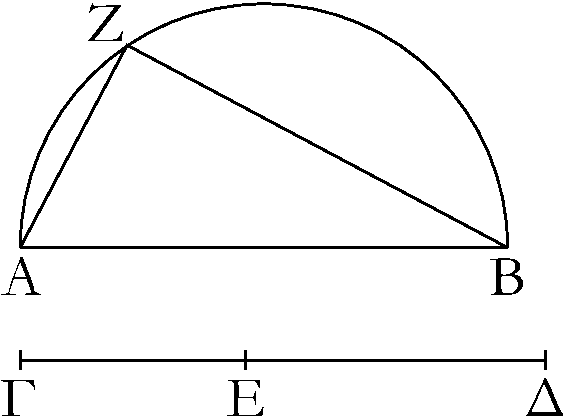
\includegraphics{Book10/fig030g.pdf}}

\gr{Ἐκκείσθω <ρητὴ ἡ ΑΒ καὶ δύο τετράγωνοι ἀριθμοὶ
οἱ ΓΕ, ΕΔ, <ώστε τὸν συγκείμενον ἐχ α\kern -.7pt  ὐτῶν τὸν ΓΔ μ\kern -.7pt  ὴ
ε>ῖναι τετράγωνον, καὶ γεγράφθω ἐπὶ τῆξ ΑΒ ἡμικύκλιον
τὸ ΑΖΒ, καὶ πεποιήσθω ὡξ ὁ ΔΓ πρὸξ τὸν ΓΕ, ο<ύτωξ
τὸ ἀπὸ τῆξ ΒΑ πρὸξ τὸ ἀπὸ τῆξ ΑΖ, καὶ ἐπεζεύθθω ἡ ΖΒ.}

\gr{Ὁμοίωξ δὴ δείχομεν τῶ| πρὸ τούτου, <ότι αἱ ΒΑ, ΑΖ <ρηταί
εἰσι δυνάμει μόνον σύμμετροι. καὶ ἐπεί ἐστιν ὡξ ὁ
ΔΓ πρὸξ τὸν ΓΕ, ο<ύτωξ τὸ ἀπὸ τῆξ ΒΑ πρὸξ τὸ ἀπὸ τῆξ
ΑΖ, ἀναστρέψαντι >άρα ὡξ ὁ ΓΔ πρὸξ τὸν ΔΕ, ο<ύτωξ τὸ ἀπὸ
τῆξ ΑΒ πρὸξ τὸ ἀπὸ τῆξ ΒΖ. ὁ δὲ ΓΔ πρὸξ τὸν ΔΕ λόγον
οὐκ >έθει, <ὸν τετράγωνοξ ἀριθμὸξ πρὸξ τετράγωνον ἀριθμόν;
οὐδ> >άρα τὸ ἀπὸ τῆξ ΑΒ πρὸξ τὸ ἀπὸ τῆξ ΒΖ λόγον
>έθει, <ὸν τετράγωνοξ ἀριθμὸξ πρὸξ τετράγωνον ἀριθμόν;
ἀσύμμετροξ >άρα ἐστὶν ἡ ΑΒ τῆ| ΒΖ μ\kern -.7pt  ήκει. καὶ δύναται
ἡ ΑΒ τῆξ ΑΖ μεῖζον τῶ| ἀπὸ τῆξ ΖΒ ἀσυμμέτρου
ἑαυτῆ|.}

\gr{Αἱ ΑΒ, ΑΖ >άρα <ρηταί εἰσι δυνάμει μόνον σύμμετροι, καὶ
ἡ ΑΒ τῆξ ΑΖ μεῖζον δύναται τῶ| ἀπὸ τῆξ ΖΒ
ἀσυμμέτρου ἑαυτῆ| μ\kern -.7pt  ήκει; <όπερ >έδει δεῖχαι.}}

\ParallelRText{
\begin{center}
{\large Proposition 30}
\end{center}

To find two rational (straight-lines which are)
commensurable in square only, such that the square on the greater
is larger than the (the square on)  lesser by the (square) on (some
straight-line which is) incommensurable in length with the greater.

% Removed epsf size command
\centerline{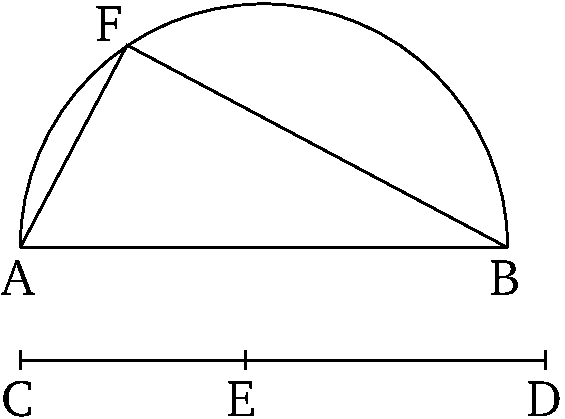
\includegraphics{Book10/fig030e.pdf}}

Let the rational (straight-line) $AB$ be laid out, and the two square
numbers, $CE$ and $ED$, such that the sum of them, $CD$,
is not square [Prop.~10.28~lem.~II].
And let the semi-circle $AFB$ be drawn on $AB$. And let it
be contrived that as $DC$ (is) to $CE$, so the (square) on
$BA$ (is) to the (square) on $AF$ [Prop.~10.6~corr].
And let $FB$ be joined.

So, similarly to the (proposition) before this, we can show that $BA$ and
$AF$ are rational (straight-lines which are) commensurable in square only.
And since as $DC$ is to $CE$, so the (square) on $BA$ (is) to the (square)
on $AF$, thus, via conversion, as $CD$ (is) to $DE$, so the (square) on
$AB$ (is) to the (square) on $BF$ [Props.~5.19~corr., 3.31, 1.47]. And
$CD$ does not have to $DE$ the ratio which (some) square number
(has) to (some) square number. Thus, the (square) on $AB$
does not have to the (square) on $BF$ the ratio which (some)
square number has to (some) square number either. Thus, $AB$ is
incommensurable in length with $BF$ [Prop.~10.9].
And the square on $AB$ is greater than the (square on) $AF$ by the
(square) on $FB$  [Prop.~1.47], (which is) incommensurable (in length) with ($AB$).

Thus, $AB$ and $AF$ are rational (straight-lines which are) commensurable
in square only, and the square on $AB$ is greater than (the square on) $AF$
by the (square) on $FB$, (which is) incommensurable (in length) with
 $(AB)$.$^\dag$ (Which is) the very thing it was required to show.}
\end{Parallel}
{\footnotesize\noindent$^\dag$ $AB$ and $AF$ have lengths $1$ and $1/\sqrt{1+k^2}$
times that of $AB$, respectively, where $k=\sqrt{DE/CE}$.}

%%%%%%
% Prop 10.31
%%%%%%
\pdfbookmark[1]{Proposition 10.31}{pdf10.31}
\begin{Parallel}{}{} 
\ParallelLText{
\begin{center}
{\large \ggn{31}.}
\end{center}\vspace*{-7pt}

\gr{Εὑρεῖν δύο μέσαξ δυνάμει μόνον συμμέτρουξ <ρητὸν περιεθούσαξ,
<ώστε τὴν μείζονα τῆξ ἐλάσσονοξ μεῖζον δύνασθαι τῶ| ἀπὸ
συμμέτρου ἑαυτῆ| μ\kern -.7pt  ήκει.}\\~\\

% Removed epsf size command
\centerline{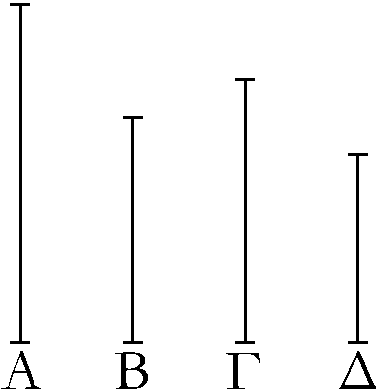
\includegraphics{Book10/fig031g.pdf}}

\gr{Ἐκκείσθωσαν δύο <ρηταὶ δυνάμει μόνον σύμμετροι αἱ Α, Β,
<ώστε τὴν Α μείζονα ο>ῦσαν τῆξ ἐλάσσονοξ τῆξ Β μεῖζον
δύνασθαι τῶ| ἀπὸ συμμέτρου ἑαυτῆ| μ\kern -.7pt  ήκει. καὶ τῶ| ὑπὸ
τῶν Α, Β >ίσον >έστω τὸ ἀπὸ τῆξ Γ. μέσον δὲ τὸ ὑπὸ
τῶν Α, Β; μέσον >άρα καὶ τὸ ἀπὸ τῆξ Γ; μέση >άρα καὶ ἡ Γ.
τῶ| δὲ ἀπὸ τῆξ Β >ίσον >έστω τὸ ὑπὸ τῶν Γ, Δ; <ρητὸν
δὲ τὸ ἀπὸ τῆξ Β; <ρητὸν >άρα καὶ τὸ ὑπὸ τῶν Γ, Δ. καὶ
ἐπεί ἐστιν ὡξ ἡ Α πρὸξ τὴν Β, ο<ύτωξ
τὸ ὑπὸ τῶν Α, Β πρὸξ τὸ ἀπὸ τῆξ Β, ἀλλὰ τῶ| μὲν
ὑπὸ τῶν Α, Β >ίσον ἐστὶ τὸ ἀπὸ τῆξ Γ, τῶ| δὲ ἀπὸ
τῆξ Β >ίσον τὸ ὑπὸ τῶν Γ, Δ, ὡξ >άρα ἡ Α πρὸξ τὴν Β,
ο<ύτωξ τὸ ἀπὸ τῆξ Γ πρὸξ τὸ ὑπὸ τῶν Γ, Δ. ὡξ δὲ
τὸ ἀπὸ τῆξ Γ πρὸξ τὸ ὑπὸ τῶν Γ, Δ, ο<ύτωξ ἡ Γ πρὸξ τὴν
Δ; καὶ ὡξ >άρα ἡ Α πρὸξ τὴν Β, ο<ύτωξ ἡ Γ πρὸξ τὴν Δ.
 σύμμετροξ δὲ ἡ Α τῆ| Β δυνάμει μόνον; σύμμετροξ
>άρα καὶ ἡ Γ τῆ| Δ δυνάμει μόνον. καί ἐστι μέση ἡ Γ;
μέση >άρα καὶ ἡ Δ. καὶ ἐπεί ἐστιν ὡξ ἡ Α πρὸξ τὴν
Β, ἡ Γ πρὸξ τὴν Δ, ἡ δὲ Α τῆξ Β μεῖζον δύναται τῶ|
ἀπὸ συμμέτρου ἑαυτῆ|, καὶ ἡ Γ >άρα τῆξ Δ μεῖζον
δύναται τῶ| ἀπὸ συμμέτρου ἑαυτῆ|.}

\gr{Ε<ύρηνται >άρα δύο μέσαι δυνάμει μόνον σύμμετροι
αἱ Γ, Δ <ρητὸν περιέθουσαι, καὶ ἡ Γ τῆξ Δ μεῖζον δυνάται
τῶ| ἀπὸ συμμέτρου ἑαυτῆ| μ\kern -.7pt  ήκει.}

\gr{Ὁμοίωξ δὴ δειθθήσεται καὶ τῶ| ἀπὸ ἀσυμμέτρου,
<όταν ἡ Α τῆξ Β μεῖζον δύνηται τῶ| ἀπὸ ἀσυμμέτρου
ἑαυτῆ|.}}

\ParallelRText{
\begin{center}
{\large Proposition 31}
\end{center}

To find two medial (straight-lines),
commensurable in square only, (and) containing a rational (area), such that
the square on the greater is larger than the (square on the) lesser by the
(square) on (some straight-line) commensurable in length with the greater.

% Removed epsf size command
\centerline{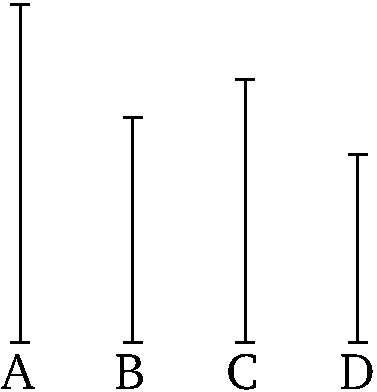
\includegraphics{Book10/fig031e.pdf}}

Let two rational (straight-lines), $A$ and $B$, commensurable in square only, 
be laid out, such that the square on the greater $A$ is larger than the (square on
the) lesser $B$ by the (square) on (some straight-line) commensurable
in length with ($A$) [Prop.~10.29]. And let the
(square) on $C$ be equal to the (rectangle contained) by $A$ and $B$.
And the (rectangle contained by) $A$ and $B$ (is) medial [Prop.~10.21]. Thus, the (square) on $C$ (is)
also medial. Thus, $C$ (is) also medial [Prop.~10.21]. And let the (rectangle contained) by $C$ and $D$
be equal to the (square) on $B$. And the (square)
on $B$ (is) rational. Thus, the (rectangle contained) by $C$ and $D$ (is)
also rational. And since as $A$ is to $B$, so the (rectangle contained) by
$A$ and $B$ (is) to the (square) on $B$ [Prop.~10.21~lem.], but the (square) on $C$
is equal to the (rectangle contained) by $A$ and $B$,  
and the (rectangle contained) by $C$ and $D$ to the (square) on
$B$, thus as $A$ (is) to $B$,
so the (square) on $C$ (is) to the (rectangle contained) by $C$ and $D$.
And as the (square) on $C$ (is) to the (rectangle contained) by $C$ and $D$,
so $C$ (is) to $D$ [Prop.~10.21~lem.].
And thus as $A$ (is) to $B$, so $C$ (is) to $D$. And $A$ is commensurable
in square only with $B$. Thus, $C$ (is) also commensurable in square
only with $D$ [Prop.~10.11]. And $C$ is medial.
Thus, $D$ (is) also medial [Prop.~10.23]. 
And since as $A$ is to $B$, (so) $C$ (is) to $D$, and the square on $A$
is greater than (the square on) $B$ by the (square) on (some straight-line)
commensurable (in length) with ($A$), the square on $C$
is thus also greater than (the square on) $D$ by the (square) on (some straight-line)
commensurable (in length) with ($C$) [Prop.~10.14]. 

Thus, two medial (straight-lines), $C$ and $D$, 
commensurable in square only, (and) containing a rational (area), be found. And the square on $C$ is greater than (the square on) $D$ by the
(square) on (some straight-line) commensurable in length with ($C$).$^\dag$

So, similarly, (the proposition) can also be demonstrated for  (some straight-line) incommensurable
(in length with $C$), provided that the square on $A$ is greater than (the square on $B$) by the (square) on (some straight-line) incommensurable (in length) with ($A$) [Prop.~10.30].$^\ddag$}
\end{Parallel}
{\footnotesize\noindent$^\dag$ $C$ and $D$ have lengths $(1-k^2)^{1/4}$ and $(1-k^2)^{3/4}$ times that of $A$, respectively, where $k$ is defined in the
footnote to Prop.~10.29.\\[0.5ex]
$^\ddag$ $C$ and $D$ would have lengths $1/(1+k^2)^{1/4}$ and $1/(1+k^2)^{3/4}$ times that of $A$, respectively, where $k$ is defined in the footnote to  Prop.~10.30.}

%%%%%%
% Prop 10.32
%%%%%%
\pdfbookmark[1]{Proposition 10.32}{pdf10.32}
\begin{Parallel}{}{} 
\ParallelLText{
\begin{center}
{\large \ggn{32}.}
\end{center}\vspace*{-7pt}

\gr{Εὑρεῖν δύο μέσαξ δυνάμει μόνον συμμέτρουξ μέσον περιεθούσαξ,
<ώστε τὴν μείζονα τῆξ ἐλάσσονοξ μεῖζον δύνασθαι τῶ| ἀπὸ
συμμέτρου ἑαυτῆ|.}\\~\\

% Removed epsf size command
\centerline{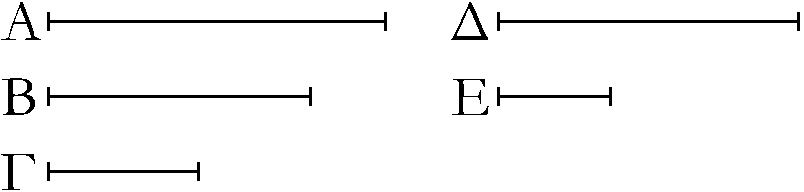
\includegraphics{Book10/fig032g.pdf}}

\gr{Ἐκκείσθωσαν τρεῖξ <ρηταὶ δυνάμει μόνον σύμμετροι αἱ Α, Β, Γ,
<ώστε τὴν Α τῆξ Γ μεῖζον δύνασθαι τῶ| ἀπὸ συμμέτρου
ἑαυτῆ|, καὶ τῶ| μὲν ὑπὸ τῶν Α, Β >ίσον >έστω τὸ ἀπὸ
τὴξ Δ. μέσον >άρα τὸ ἀπὸ τῆξ Δ; καὶ ἡ Δ >άρα μέση ἐστίν.
τῶ| δὲ ὑπὸ τῶν Β, Γ >ίσον >έστω τὸ ὑπὸ τῶν Δ, Ε. καὶ
ἐπεί ἐστιν ὡξ τὸ ὑπὸ τῶν Α, Β πρὸξ τὸ ὑπὸ τῶν Β, Γ, ο<ύτωξ
ἡ Α πρὸξ τὴν Γ, ἀλλὰ τῶ| μὲν ὑπὸ τῶν Α, Β >ίσον ἐστὶ τὸ
ἀπὸ τῆξ Δ, τῶ| δὲ ὑπὸ τῶν Β, Γ >ίσον τὸ ὑπὸ τῶν Δ, Ε, >έστιν
>άρα ὡξ ἡ Α πρὸξ τὴν Γ, ο<ύτωξ τὸ ἀπὸ τῆξ Δ πρὸξ
τὸ ὑπὸ τῶν Δ, Ε. ὡξ δὲ τὸ ἀπὸ τῆξ Δ πρὸξ τὸ ὑπὸ
τῶν Δ, Ε, ο<ύτωξ ἡ Δ πρὸξ τὴν Ε; καὶ ὡξ >άρα ἡ Α πρὸξ τὴν
Γ, ο<ύτωξ ἡ Δ πρὸξ τὴν Ε. σύμμετροξ δὲ ἡ Α τῆ| Γ δυνάμει [μόνον].
σύμμετροξ >άρα καὶ ἡ Δ τῆ| Ε δυνάμει μόνον. μέση δὲ ἡ Δ;
μέση >άρα καὶ ἡ Ε. καὶ ἐπεί ἐστιν ὡξ ἡ Α πρὸξ τὴν Γ, ἡ Δ πρὸξ
τὴν Ε, ἡ δὲ Α τῆξ Γ μεῖζον δύναται τῶ| ἀπὸ συμμέτρου
ἑαυτῆ|, καὶ ἡ Δ >άρα τῆξ Ε μεῖζον δυνήσεται τῶ| ἀπὸ
συμμέτρου ἑαυτῆ|. λέγω δή, <ότι καὶ μέσον ἐστὶ τὸ ὑπὸ
τῶν Δ, Ε. ἐπεὶ γὰρ >ίσον ἐστὶ τὸ ὑπὸ τῶν
Β, Γ τῶ| ὑπὸ τῶν Δ, Ε, μέσον δὲ τὸ ὑπὸ τῶν Β, Γ [αἱ γὰρ
Β, Γ <ρηταί εἰσι δυνάμει μόνον σύμμετροι], μέσον >άρα καὶ
τὸ ὑπὸ τῶν Δ, Ε.}

\gr{Ε<ύρηνται >άρα δύο μέσαι δυνάμει μόνον σύμμετροι αἱ Δ, Ε
μέσον περιέθουσαι, <ώστε τὴν μείζονα τῆξ ἐλάσσονοξ
μεῖζον δύνασθαι τῶ| ἀπὸ συμμέτρου ἑαυτῆ|.}

\gr{Ὁμοίωξ δὴ πάλιν διεθθήσεται καὶ τῶ| ἀπὸ ἀσυμμέτρ\-ου, <όταν
ἡ Α τῆξ Γ μεῖζον δύνηται τῶ| ἀπὸ ἀσυμμέτρου ἑαυτῃ.}}

\ParallelRText{
\begin{center}
{\large Proposition 32}
\end{center}

To find two medial (straight-lines), commensurable in square only, (and) containing a medial (area), such that
the square on the greater is larger than the (square on the) lesser by the
(square) on (some straight-line) commensurable (in length) with the greater.

% Removed epsf size command
\centerline{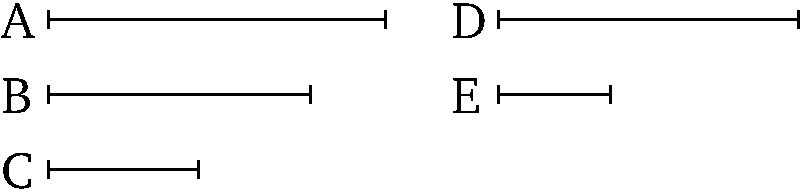
\includegraphics{Book10/fig032e.pdf}}

Let three rational (straight-lines), $A$, $B$ and $C$, commensurable
in square only, be laid out such that the square on $A$ is greater
than (the square on $C$) by the (square) on (some straight-line)
commensurable (in length) with ($A$) [Prop.~10.29].
And let the (square) on $D$ be equal to the (rectangle contained) by $A$ and
$B$. Thus, the (square) on $D$ (is) medial. Thus, $D$ is also
medial [Prop.~10.21].  And let the 
(rectangle contained) by $D$ and $E$ be equal to the (rectangle contained)
by $B$ and $C$. And since as the (rectangle contained) by $A$ and $B$
is to the (rectangle contained) by $B$ and $C$, so $A$ (is) to $C$
[Prop.~10.21~lem.], but the (square) on $D$
is equal to the (rectangle contained) by $A$ and $B$, and the
(rectangle contained) by $D$ and $E$ to the (rectangle contained) by
$B$ and $C$, thus as $A$ is to $C$, so the (square) on $D$ (is) to
the (rectangle contained) by $D$ and $E$. And as the (square) on $D$
(is) to the (rectangle contained) by $D$ and $E$, so $D$ (is) to $E$ [Prop.~10.21~lem.]. And thus as
$A$ (is) to $C$, so $D$ (is) to $E$. And $A$ (is) commensurable in square
[only] with $C$. Thus, $D$ (is) also commensurable in square only
with $E$ [Prop.~10.11]. And $D$ (is) medial.
Thus, $E$ (is) also medial [Prop.~10.23]. And
since as $A$ is to $C$, (so) $D$ (is) to $E$, and the square on $A$
is greater than (the square on) $C$ by the (square)
on (some straight-line) commensurable (in length) with ($A$),  the square on $D$
will thus also be greater than (the square on) $E$ by the (square) on (some straight-line)
commensurable (in length) with ($D$) [Prop.~10.14].
So, I also say that the (rectangle contained) by $D$ and $E$ is medial.
For since the (rectangle contained) by $B$ and $C$ is equal to the
(rectangle contained) by $D$ and $E$, and the (rectangle contained)
by $B$ and $C$ (is) medial [for $B$ and $C$ are rational
(straight-lines which are) commensurable in square only] [Prop.~10.21], the (rectangle contained) by $D$ and
$E$ (is) thus also medial.

Thus, two medial (straight-lines), $D$ and $E$, commensurable in square only, (and) containing a medial (area), be found such that
the square on the greater is larger than the (square on the) lesser by the
(square) on (some straight-line) commensurable (in length) with the greater.$^\dag$.

So, similarly, (the proposition) can again also be demonstrated for
(some straight-line) incommensurable (in length with the greater), provided that
the square on $A$ is greater than (the square on) $C$ by the (square)
on (some straight-line) incommensurable (in length) with ($A$) [Prop.~10.30].$^\ddag$}
\end{Parallel}
{\footnotesize\noindent $^\dag$ $D$ and $E$ have lengths $k'^{1/4}$ and $k'^{1/4}\sqrt{1-k^2}$ times that of $A$, respectively, where the length of $B$ is $k'^{1/2}$ times that of $A$, and $k$ is defined in the footnote to
Prop.~10.29.\\[0.5ex]
$^\ddag$ $D$ and $E$ would have lengths $k'^{1/4}$ and $k'^{1/4}/\sqrt{1+k^2}$ times that of $A$, respectively, where the length of $B$ is $k'^{1/2}$ times that of $A$, and $k$ is defined in the footnote to
Prop.~10.30.}

%%%%%%
% Prop 10.32a
%%%%%%
\begin{Parallel}{}{} 
\ParallelLText{
\begin{center}
{\large \gr{Λῆμμα}.}
\end{center}\vspace*{-7pt}

\gr{>'Εστω τρίγωνον ὀρθογώνιον τὸ ΑΒΓ ὀρθὴν >έθον τὴν Α, καὶ
>ήθθω κάθετοξ ἡ ΑΔ; λέγω, <ότι τὸ μὲν ὑπὸ τῶν
ΓΒΔ >ίσον ἐστὶ τῶ| ἀπὸ τῆξ ΒΑ, τὸ δὲ ὑπὸ τῶν ΒΓΑ
>ίσον τῶ| ἀπὸ τῆξ ΓΑ, καὶ τὸ ὑπὸ τῶν ΒΔ, ΔΓ >ίσον τῶ|
ἀπὸ τῆξ ΑΔ, καὶ >έτι τὸ ὑπὸ τῶν ΒΓ, ΑΔ >ίσον [ἐστὶ]
τῶ| ὑπὸ τῶν ΒΑ, ΑΓ.}

\gr{Καὶ πρῶτον, <ότι τὸ ὑπὸ τῶν ΓΒΔ >ίσον [ἐστὶ] τῶ|
ἀπὸ τῆξ ΒΑ.}\\~\\~\\

% Removed epsf size command
\centerline{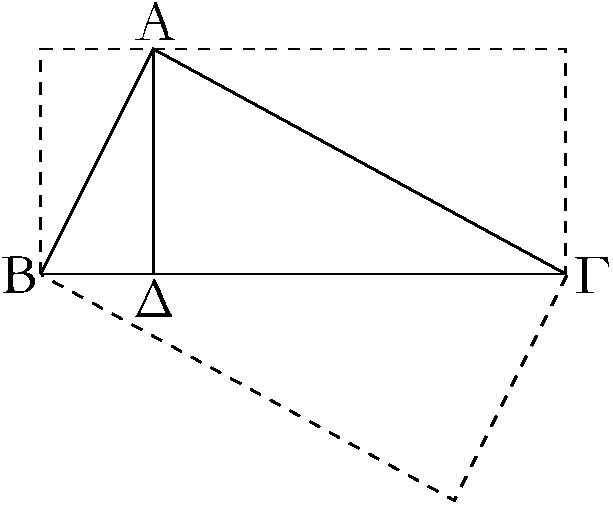
\includegraphics{Book10/fig032ag.pdf}}

\gr{Ἐπεὶ γὰρ ἐν ὀρθογωνίῳ τριγώνῳ ἀπὸ τῆξ ὀρθῆξ γωνίαξ
ἐπὶ τὴν βάσιν κάθετοξ >ῆκται ἡ ΑΔ, τὰ ΑΒΔ, ΑΔΓ >άρα τρίγωνα
<όμοιά ἐστι τῶ| τε <όλῳ τῶ| ΑΒΓ καὶ ἀλλήλοιξ. καὶ ἐπεὶ
<όμοιόν ἐστι τὸ ΑΒΓ τρίγωνον τῶ| ΑΒΔ τριγώνῳ, >έστιν
>άρα ὡξ ἡ ΓΒ πρὸξ τὴν ΒΑ, ο<ύτωξ ἡ ΒΑ πρὸξ τὴν ΒΔ;
τὸ >άρα ὑπὸ τῶν ΓΒΔ >ίσον ἐστὶ τῶ| ἀπὸ τῆξ ΑΒ.}

\gr{Διὰ τὰ α\kern -.7pt  ὐτὰ δὴ καὶ τὸ ὑπὸ τῶν ΒΓΔ >ίσον ἐστὶ τῶ|
ἀπὸ τῆξ ΑΓ.}

\gr{Καὶ ἐπεί, ἒαν ἐν ὀρθογωνίῳ τριγώνῳ ἀπὸ τῆξ ὀρθῆξ
γωνίαξ ἐπὶ τὴν βάσιν κάθετοξ ἀθθῆ|, ἡ ἀθθεῖσα τῶν τῆξ
βάσεωξ τμ\kern -.7pt  ημάτων μέση ἀνάλογόν ἐστιν, >έστιν >άρα ὡξ ἡ
ΒΑ πρὸξ τὴν ΔΑ, ο<ύτωξ ἡ ΑΔ πρὸξ τὴν ΔΓ; τὸ >άρα ὑπὸ
τῶν ΒΔ, ΔΓ >ίσον ἐστὶ τῶ| ἀπὸ τῆξ ΔΑ.}

\gr{Λέγω, <ότι καὶ τὸ ὑπὸ τῶν ΒΓ, ΑΔ >ίσον ἐστὶ τῶ| ὑπὸ
τῶν ΒΑ, ΑΓ. ἐπεὶ γὰρ, ὡξ >έφαμεν, <όμοιόν ἐστι
τὸ ΑΒΓ τῶ| ΑΒΔ, >έστιν >άρα ὡξ ἡ ΒΓ πρὸξ τὴν ΓΑ,
ο<ύτωξ ἡ ΒΑ πρὸξ τὴν ΑΔ. τὸ >άρα ὑπὸ τῶν ΒΓ, ΑΔ >ίσον
ἐστὶ τῶ| ὑπὸ τῶν ΒΑ, ΑΓ; <όπερ >έδει δεῖχαι.}}

\ParallelRText{
\begin{center}
{\large Lemma}
\end{center}

Let $ABC$ be a right-angled triangle having
the (angle) $A$ a right-angle. And let the perpendicular $AD$ be
drawn. I say that the (rectangle contained) by $CBD$ is equal to the
(square) on $BA$, and the (rectangle contained) by $BCD$ (is)
equal to the (square) on $CA$, and the (rectangle contained) by
$BD$ and $DC$ (is) equal to the (square) on $AD$, and, further, the
(rectangle contained) by $BC$ and $AD$ [is] equal to the (rectangle
contained) by $BA$ and $AC$.

And, first of all, (let us prove) that the (rectangle contained) by
$CBD$ [is] equal to the (square) on $BA$.

% Removed epsf size command
\centerline{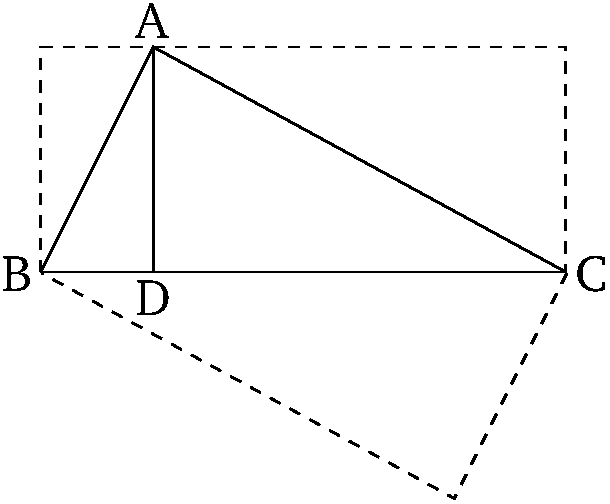
\includegraphics{Book10/fig032ae.pdf}}

For since $AD$ has been drawn from the right-angle  in a right-angled triangle,
perpendicular to the base, $ABD$ and $ADC$ are thus
triangles (which are) similar to the whole, $ABC$, and to one another
[Prop.~6.8]. And since triangle $ABC$ is
similar to triangle $ABD$, thus as $CB$ is to $BA$, so $BA$ (is)
to $BD$ [Prop.~6.4]. Thus, the
(rectangle contained) by $CBD$ is equal to the (square) on $AB$
[Prop.~6.17].

So, for the same (reasons), the (rectangle contained) by $BCD$
is also equal to the (square) on $AC$.

And since if a (straight-line) is drawn from the right-angle in a right-angled
triangle,  perpendicular to the base, the (straight-line so) drawn
is the mean proportional to the pieces of the base [Prop.~6.8~corr.], thus as $BD$ is to $DA$, so $AD$ (is) to $DC$. Thus, the (rectangle contained) by
$BD$ and $DC$ is equal to the (square) on $DA$ [Prop.~6.17]. 

I also say that the (rectangle contained) by $BC$ and
$AD$ is equal to the (rectangle contained) by $BA$ and $AC$.
For since,  as we said, $ABC$ is similar to $ABD$, thus as $BC$
is to $CA$, so $BA$ (is) to $AD$ [Prop.~6.4].
Thus, the (rectangle contained) by $BC$ and $AD$
is equal to the (rectangle contained) by $BA$ and $AC$ [Prop.~6.16].
(Which is) the very thing it was required to show.}
\end{Parallel}

%%%%%%
% Prop 10.33
%%%%%%
\pdfbookmark[1]{Proposition 10.33}{pdf10.33}
\begin{Parallel}{}{} 
\ParallelLText{
\begin{center}
{\large \ggn{33}.}
\end{center}\vspace*{-7pt}

\gr{Εὑρεῖν δύο εὐθείαξ δυνάμει ἀσυμμέτρουξ ποιούσαξ τὸ μὲν συγκείμενον ἐκ τῶν ἀπ> α\kern -.7pt  ὐτῶν τετραγώνων <ρητόν, τὸ
δ> ὑπ> α\kern -.7pt  ὐτῶν μέσον.}

\gr{Ἐκκείσθωσαν δύο <ρηταὶ δυνάμει μόνον σύμμετροι αἱ
ΑΒ, ΒΓ, <ώστε τὴν μείζονα τὴν ΑΒ τῆξ ἐλάσσονοξ
τῆξ ΒΓ μείζον δύνασθαι τῶ| ἀπὸ ἀσυμμέτρου ἑαυτῆ|,
καὶ τετμ\kern -.7pt  ήσθω ἡ ΒΓ δίθα κατὰ τὸ Δ, καὶ τῶ| ἀφ>
ὁποτέραξ τῶν ΒΔ, ΔΓ >ίσον παρὰ τὴν ΑΒ παραβεβλήσθω
παραλληλόγραμμον ἐλλεῖπον ε>ίδει τετραγώνῳ, καὶ >έστω τὸ ὑπὸ
τῶν ΑΕΒ, καὶ γεγράφθω ἐπὶ τῆξ ΑΒ ημικύκλιον τὸ ΑΖΒ, καὶ
>ήθθω τῆ| ΑΒ πρὸξ ὀρθὰξ ἡ ΕΖ, καὶ ἐπεζεύθθωσαν αἱ ΑΖ, ΖΒ.}\\~\\~\\

% Removed epsf size command
\centerline{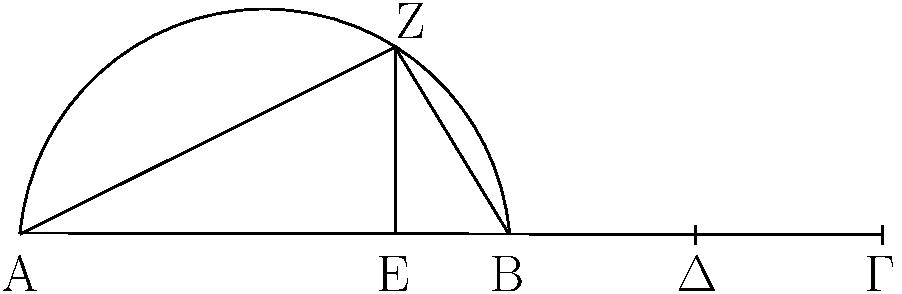
\includegraphics{Book10/fig033g.pdf}}

\gr{Καὶ ἐπεὶ [δύο] εὐθεῖαι >άνισοί εἰσιν αἱ ΑΒ, ΒΓ, καὶ ἡ ΑΒ
τῆξ ΒΓ μεῖζον δύναται τῶ| ἀπὸ ἀσυμμέτρου ἑαυτῆ|, τῶ|
δὲ τετάρτῳ τοῦ ἀπὸ τῆξ ΒΓ, τουτέστι τῶ| ἀπὸ τῆξ ἡμισείαξ
α\kern -.7pt  ὐτῆξ, >ίσον παρὰ τὴν ΑΒ παραβέβληται παραλληλόγραμμον
ἐλλεῖπον ε>ίδει τετραγώνῳ καὶ ποιεῖ τὸ ὑπὸ τῶν ΑΕΒ,
ἀσύμμετροξ >άρα ἐστὶν ἡ ΑΕ τῆ| ΕΒ. καί ἐστιν ὡξ ἡ ΑΕ πρὸξ
ΕΒ, ο<ύτωξ τὸ ὑπὸ τῶν ΒΑ, ΑΕ πρὸξ τὸ ὑπὸ τῶν ΑΒ, ΒΕ, >ίσον
δὲ τὸ μὲν ὑπὸ τῶν ΒΑ, ΑΕ τῶ| ἀπὸ τῆξ ΑΖ, τὸ δὲ ὑπὸ
τῶν ΑΒ, ΒΕ τῶ| ἁπὸ τῆξ
 ΒΖ; ἀσύμμετρον
>άρα ἐστὶ τὸ ἀπὸ τῆξ ΑΖ τῶ| ἀπὸ τῆξ ΖΒ; αἱ ΑΖ, ΖΒ
>άρα δυνάμει εἰσὶν ἀσύμμετροι. καὶ ἐπεὶ ἡ ΑΒ <ρητή ἐστιν,
<ρητὸν >άρα ἐστὶ καὶ τὸ ἀπὸ τῆξ ΑΒ; <ώστε καὶ τὸ συγκείμενον
ἐκ τῶν ἀπὸ τῶν ΑΖ, ΖΒ <ρητόν ἐστιν. καὶ ἐπεὶ πάλιν τὸ
ὑπὸ τῶν ΑΕ, ΕΒ >ίσον ἐστὶ τῶ| ἀπὸ τῆξ ΕΖ, ὑπόκειται
δὲ τὸ ὑπὸ τῶν ΑΕ, ΕΒ καὶ τῶ| ἀπὸ τῆξ ΒΔ >ίσον, >ίση
>άρα ἐστὶν ἡ ΖΕ τῆ| ΒΔ; διπλῆ >άρα ἡ ΒΓ  τὴξ ΖΕ; <ώστε
καὶ τὸ ὑπὸ τῶν ΑΒ, ΒΓ σύμμετρόν ἐστι τῶ| ὑπὸ τῶν
ΑΒ, ΕΖ. μέσον δὲ τὸ ὑπὸ τῶν ΑΒ, ΒΓ; μέσον >άρα καὶ τὸ ὑπὸ
τῶν ΑΒ, ΕΖ. >ίσον δὲ τὸ ὑπὸ τῶν ΑΒ, ΕΖ τῶ| ὑπὸ τῶν
ΑΖ, ΖΒ; μέσον >άρα καὶ τὸ ὑπὸ τῶν ΑΖ, ΖΒ. ἐδείθθη
δὲ καὶ <ρητὸν τὸ
 συγκείμενον ἐκ τῶν ἀπ>
α\kern -.7pt  ὐτῶν τετραγώνων.}

\gr{Ε<ύρηνται >άρα δύο εὐθεῖαι δυνάμει ἀσύμμετροι αἱ ΑΖ, ΖΒ ποιοῦσαι τὸ μὲν συγκείμενον ἐκ τῶν ἀπ> α\kern -.7pt  ὐτῶν τετραγώνων <ρητόν,
τὸ δὲ ὑπ> α\kern -.7pt  ὐτῶν μέσον; <όπερ >έδει δεῖχαι.}}

\ParallelRText{
\begin{center}
{\large Proposition 33}
\end{center}

To find two straight-lines (which are) incommensurable
in square, making the sum of the squares on them rational, and the (rectangle contained) by them medial.

Let the two rational (straight-lines) $AB$ and $BC$, (which are) commensurable in square only, be laid out such that the square on the greater, $AB$, is larger
than (the square on) the lesser, $BC$, by the (square) on (some straight-line which is) incommensurable (in length)
with ($AB$) [Prop.~10.30]. And let $BC$ be
cut in half at $D$. And let a parallelogram equal to the (square) on
either of $BD$ or $DC$, (and) falling short by a square figure, 
be applied to $AB$ [Prop.~6.28], and
let it be the (rectangle contained) by $AEB$. And let the semi-circle
$AFB$ be drawn on $AB$. And let $EF$ be
drawn at right-angles to $AB$. And let $AF$ and $FB$ be joined.

% Removed epsf size command
\centerline{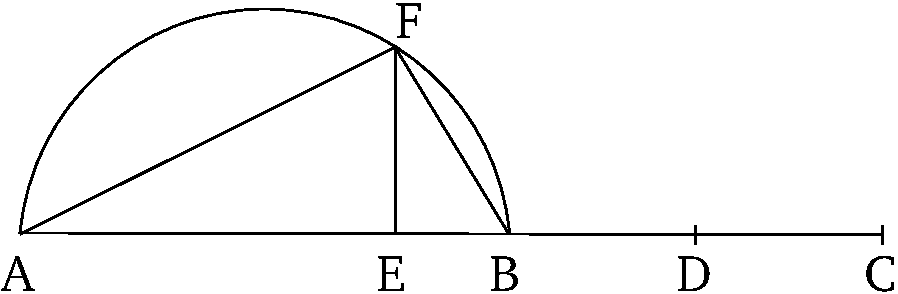
\includegraphics{Book10/fig033e.pdf}}

And since $AB$ and $BC$ are [two] unequal straight-lines, and the square
on $AB$ is greater than (the square on) $BC$ by the (square) on (some
straight-line which is) incommensurable (in length) with ($AB$). And a parallelogram,
equal to one quarter of the (square) on $BC$---that is to say, (equal) to the
(square) on half of it---(and) falling short by a square figure, has
been applied to $AB$, and  makes the (rectangle contained) by $AEB$.
$AE$ is thus incommensurable (in length) with $EB$ [Prop.~10.18]. And as $AE$ is to $EB$, so the
(rectangle contained) by $BA$ and $AE$ (is) to the (rectangle contained) by
$AB$ and $BE$.
 And the (rectangle contained) by $BA$ and $AE$ (is) equal to the (square) on $AF$, and the (rectangle contained) by $AB$ and $BE$ to the (square) on
$BF$ [Prop.~10.32~lem.]. The (square) on
$AF$ is thus incommensurable with the (square) on $FB$ [Prop.~10.11]. Thus, $AF$ and $FB$ are
incommensurable in square. And since $AB$ is rational,
the (square) on $AB$ is also rational. Hence, the sum of the
(squares) on $AF$ and $FB$ is also rational [Prop.~1.47]. And, again, since the (rectangle
contained) by $AE$ and $EB$ is equal to the (square) on $EF$, and
the (rectangle contained) by $AE$ and $EB$ 
was assumed (to be) equal to the (square) on $BD$, $FE$ is thus equal to $BD$. Thus, $BC$
is double $FE$. And hence the (rectangle contained) by $AB$ and $BC$ is commensurable with the (rectangle contained) by $AB$ and $EF$ [Prop.~10.6]. And the (rectangle contained) by
$AB$ and $BC$ (is) medial [Prop.~10.21]. 
Thus, the (rectangle contained) by $AB$ and $EF$ (is) also medial
[Prop.~10.23~corr.].  And the (rectangle contained)
by $AB$ and $EF$ (is) equal to the (rectangle contained) by $AF$ and $FB$
[Prop.~10.32~lem.]. Thus, the (rectangle
contained) by $AF$ and $FB$ (is) also medial. And the
sum of the squares on them was also shown (to be) rational.

Thus, the two straight-lines, $AF$ and $FB$, (which are)
incommensurable in  square, be found, making the
sum of the squares on them rational, and the (rectangle contained)
by them medial. (Which is) the very thing it was required to show.}
\end{Parallel}
{\footnotesize\noindent$^\dag$ $AF$ and $FB$ have lengths
$\sqrt{[1+k/(1+k^2)^{1/2}]/2}$ and $\sqrt{[1-k/(1+k^2)^{1/2}]/2}$
times that of $AB$, respectively, where $k$ is defined in the footnote
to Prop.~10.30.}

%%%%%%
% Prop 10.34
%%%%%%
\pdfbookmark[1]{Proposition 10.34}{pdf10.34}
\begin{Parallel}{}{} 
\ParallelLText{
\begin{center}
{\large \ggn{34}.}
\end{center}\vspace*{-7pt}

\gr{Εὑρεῖν δύο εὐθείαξ δυνάμει ἀσυμμέτρουξ ποιούσαξ τὸ μὲν
συγκείμενον ἐκ τῶν ἀπ> α\kern -.7pt  ὐτῶν τετραγώνων μέσον, τὸ δ>
ὑπ> α\kern -.7pt  ὐτῶν <ρητόν.}

% Removed epsf size command
\centerline{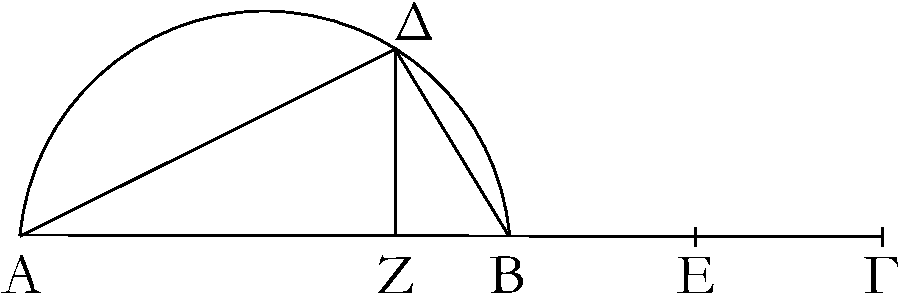
\includegraphics{Book10/fig034g.pdf}}

\gr{Ἐκκείσθωσαν δύο μέσαι δυνάμει μόνον σύμμετροι αἱ ΑΒ, ΒΓ <ρητὸν
περιέθουσαι τὸ ὑπ> α\kern -.7pt  ὐτῶν, <ώστε τὴν ΑΒ τῆξ ΒΓ μεῖζον δύνασθαι
τῶ| ἀπὸ ἀσυμμέτρου ἑαυτῆ|, καὶ γεγράφθω ἐπὶ τῆξ ΑΒ τὸ
ΑΔΒ ἡμικύκλιον, καὶ τετμ\kern -.7pt  ήσθω ἡ ΒΓ δίθα κατὰ τὸ Ε, καὶ
παραβεβλήσθω παρὰ τὴν ΑΒ τῶ| ἀπὸ τῆξ ΒΕ >ίσον
παραλληλόγραμμον ἐλλεῖπον ε>ίδει τετραγώνῳ τὸ ὑπὸ τῶν ΑΖΒ;
ἀσύμμετροξ >άρα [ἐστὶν] ἡ ΑΖ τῆ| ΖΒ μ\kern -.5pt  ήκει. καὶ >ήθθω ἀπὸ
τοῦ Ζ τῆ| ΑΒ πρὸξ ὀρθὰξ ἡ ΖΔ, καὶ ἐπεζεύθθωσαν αἱ ΑΔ, ΔΒ.}

\gr{Ἐπεὶ ἀσύμμετρόξ ἐστιν ἡ ΑΖ τῆ| ΖΒ, ἀσύμμετρον
>άρα ἐστὶ καὶ τὸ ὑπὸ τῶν ΒΑ, ΑΖ τῶ| ὑπὸ τῶν
ΑΒ, ΒΖ. >ίσον δὲ τὸ μὲν ὑπὸ τῶν ΒΑ, ΑΖ τῶ| ἀπὸ τῆξ
ΑΔ, τὸ δὲ ὑπὸ τῶν ΑΒ, ΒΖ τῶ| ἀπὸ τῆξ ΔΒ; ἀσύμμετρον
>άρα ἐστὶ καὶ τὸ ἀπὸ τῆξ ΑΔ τῶ| ἀπὸ τῆξ ΔΒ.
καὶ ἐπεὶ μέσον ἐστὶ τὸ ἀπὸ τῆξ ΑΒ, μέσον >άρα καὶ τὸ
συγκείμενον ἐκ τῶν ἀπὸ τῶν ΑΔ, ΔΒ. καὶ ἐπεὶ διπλῆ
ἐστιν ἡ ΒΓ τῆξ ΔΖ, διπλάσιον >άρα καὶ τὸ
ὑπὸ τῶν ΑΒ, ΒΓ τοῦ ὑπὸ τῶν ΑΒ, ΖΔ. <ρητὸν δὲ τὸ ὑπὸ
τῶν ΑΒ, ΒΓ; <ρητὸν >άρα καὶ τὸ ὑπὸ τῶν ΑΒ, ΖΔ. τὸ δὲ
ὑπὸ τῶν ΑΒ, ΖΔ >ίσον τῶ| ὑπὸ
τῶν ΑΔ, ΔΒ; <ώστε καὶ τὸ ὑπὸ τῶν ΑΔ, ΔΒ <ρητόν
ἐστιν.}

\gr{Ε<ύρηνται >άρα δύο εὐθεῖαι δυνάμει ἀσύμμετροι αἱ
ΑΔ, ΔΒ ποιοῦσαι τὸ [μὲν] συγκείμενον ἐκ τῶν ἀπ>
α\kern -.7pt  ὐτῶν τετραγώνων μέσον, τὸ δ> ὑπ> α\kern -.7pt  ὐτῶν <ρητόν;
<όπερ >έδει δεῖχαι.}}

\ParallelRText{
\begin{center}
{\large Proposition 34}
\end{center}

To find two straight-lines (which are) incommensurable in square, making the sum of the squares on them medial,
and the (rectangle contained) by them rational.

% Removed epsf size command
\centerline{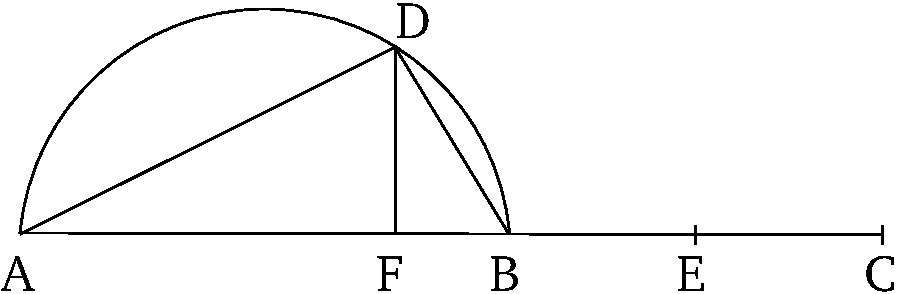
\includegraphics{Book10/fig034e.pdf}}

Let the two medial (straight-lines) $AB$ and $BC$,
(which are) commensurable in square only, be laid out having the
(rectangle contained) by them rational, (and) such that the square on
$AB$ is greater than (the square on) $BC$ by the (square) on (some straight-line)
incommensurable (in length) with ($AB$) [Prop.~10.31].
And let the semi-circle $ADB$ be drawn on $AB$.
And let $BC$ be cut in half at $E$. And let a (rectangular) parallelogram
equal to the (square) on $BE$, (and) falling short by a square figure,
be applied to $AB$, (and let it be) the (rectangle
contained by) $AFB$ [Prop.~6.28].
Thus, $AF$ [is] incommensurable in length with $FB$
[Prop.~10.18]. And let 
$FD$ be drawn from $F$ at right-angles to $AB$.
And let $AD$ and $DB$ be joined.

Since $AF$ is incommensurable (in length) with $FB$, the (rectangle contained) by
$BA$ and $AF$ is thus also incommensurable with the (rectangle contained)
by $AB$ and $BF$ [Prop.~10.11].  And the
(rectangle contained) by $BA$ and $AF$ (is) equal to the (square) on $AD$, and the (rectangle contained) by $AB$ and $BF$ to the (square) on $DB$
[Prop.~10.32~lem.]. Thus, the (square) on
$AD$ is also incommensurable with the (square) on $DB$. And
since the (square) on $AB$ is medial, the sum of the (squares) on
$AD$ and $DB$ (is) thus also medial [Props.~3.31, 1.47]. And since $BC$ is double $DF$ [see previous proposition], the (rectangle
contained) by $AB$ and $BC$ (is) thus also double the (rectangle contained)
by $AB$ and $FD$. And the (rectangle contained) by $AB$ and $BC$ (is)
rational. Thus, the (rectangle contained) by $AB$ and $FD$
(is) also rational [Prop.~10.6, Def.~10.4]. And the (rectangle contained) by
$AB$ and $FD$ (is) equal to the (rectangle contained) by $AD$ and $DB$
[Prop.~10.32~lem.]. And hence the (rectangle
contained) by $AD$ and $DB$ is rational.

Thus, two straight-lines, $AD$ and $DB$, (which are) incommensurable
in square, be found, making the sum of the squares on them medial,
and the (rectangle contained) by them rational.$^\dag$
(Which is) the very thing
it was required to show.}
\end{Parallel}
{\footnotesize\noindent$^\dag$ $AD$ and $DB$ have lengths $\sqrt{[(1+k^2)^{1/2}+k]/[2\,(1+k^2)]}$
and  $\sqrt{[(1+k^2)^{1/2}-k]/[2\,(1+k^2)]}$ times that of $AB$, respectively, where $k$ is defined in the footnote
to Prop.~10.29.}

%%%%%%
% Prop 10.35
%%%%%%
\pdfbookmark[1]{Proposition 10.35}{pdf10.35}
\begin{Parallel}{}{} 
\ParallelLText{
\begin{center}
{\large \ggn{35}.}
\end{center}\vspace*{-7pt}

\gr{Εὑρεῖν δύο εὐθείαξ δυνάμει ἀσυμμέτρουξ ποιούσαξ τό τε συγκείμενον ἐκ τῶν ἀπ> α\kern -.7pt  ὐτῶν τετραγώνων μέσον καὶ
τὸ ὑπ> α\kern -.7pt  ὐτῶν μέσον καὶ >έτι ἀσύμμετρον τῶ| συγκειμένῳ
ἐκ τῶν ἀπ> α\kern -.5pt  ὐτῶν τετραγώνῳ.}

% Removed epsf size command
\centerline{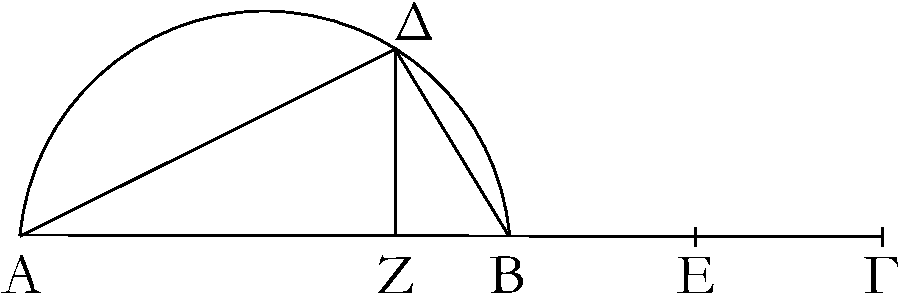
\includegraphics{Book10/fig034g.pdf}}

\gr{Ἐκκείσθωσαν δύο μέσαι δυνάμει μόνον σύμμετροι αἱ ΑΒ, ΒΓ
μέσον περιέθουσαι, <ώστε τὴν ΑΒ τῆξ ΒΓ μεῖζον δύνασθαι τῶ|
ἀπὸ ἀσυμμέτρου ἑαυτῆ|, καὶ γεγράφθω ἐπὶ τῆξ ΑΒ
ἡμικύκλιον τὸ ΑΔΒ, καὶ τὰ λοιπὰ γεγονέτω τοῖξ ἐπάνω
ὁμοίωξ.}

\gr{Καὶ ἐπεὶ ἀσύμμετρόξ ἐστιν ἡ ΑΖ τῆ| ΖΒ μ\kern -.7pt  ήκει, ἀσύμμετρ\-όξ
ἐστι καὶ ἡ ΑΔ τῆ| ΔΒ δυνάμει. καὶ ἐπεὶ μέσον ἐστὶ
τὸ ἀπὸ τῆξ ΑΒ, μέσον >άρα καὶ τὸ συγκείμενον ἐκ τῶν
ἀπὸ τῶν ΑΔ, ΔΒ. καὶ ἐπεὶ τὸ ὑπὸ τῶν ΑΖ, ΖΒ >ίσον
ἐστὶ τῶ| ἀφ> ἑκατέραξ τῶν ΒΕ, ΔΖ, >ίση >άρα
ἐστὶν ἡ ΒΕ τῆ| ΔΖ; διπλῆ >άρα ἡ ΒΓ τῆξ ΖΔ; <ώστε
καὶ τὸ ὑπὸ τῶν ΑΒ, ΒΓ διπλάσιόν ἐστι τοῦ ὑπὸ τῶν
ΑΒ, ΖΔ. μέσον δὲ τὸ ὑπὸ τῶν ΑΒ, ΒΓ; μέσον >άρα καὶ τὸ
ὑπὸ τῶν ΑΒ, ΖΔ. καί ἐστιν >ίσον τῶ| ὑπὸ τῶν ΑΔ, ΔΒ;
μέσον >άρα καὶ τὸ ὑπὸ τῶν ΑΔ, ΔΒ. καὶ ἐπεὶ ἀσύμμετρόξ
ἐστιν ἡ ΑΒ τῆ| ΒΓ μ\kern -.7pt  ήκει, σύμμετροξ δὲ ἡ ΓΒ τῆ| ΒΕ,
ἀσύμμετροξ >άρα καὶ ἡ ΑΒ τῆ| ΒΕ μ\kern -.5pt  ήκει; <ώστε καὶ τὸ ἀπὸ
τῆξ ΑΒ τῶ| ὑπὸ τῶν ΑΒ, ΒΕ ἀσύμμετρόν ἐστιν. ἀλλὰ
τῶ| μὲν ἀπὸ τῆξ ΑΒ >ίσα ἐστὶ τὰ ἀπὸ τῶν ΑΔ, ΔΒ, τῶ|
δὲ ὑπὸ τῶν ΑΒ, ΒΕ >ίσον ἐστὶ τὸ ὑπὸ τῶν ΑΒ,
ΖΔ, τουτέστι τὸ ὑπὸ τῶν ΑΔ, ΔΒ; ἀσύμμετρον >άρα
ἐστὶ τὸ συγκείμενον ἐκ τῶν ἀπὸ τῶν ΑΔ, ΔΒ
τῶ| ὑπὸ τῶν ΑΔ, ΔΒ.}

\gr{Ε<ύρηνται >άρα δύο εὐθεῖαι αἱ ΑΔ, ΔΒ δυνάμει ἀσύμμετροι
ποιοῦσαι τό τε συγκείμενον ἐκ τῶν ἀπ> α\kern -.7pt  ὐτῶν μέσον
καὶ τὸ ὑπ> α\kern -.7pt  ὐτῶν μέσον καὶ >έτι ἀσύμμετρον τῶ|
συγκειμένῳ ἐκ τῶν ἀπ> α\kern -.5pt  ὐτῶν τετραγώνων;
<όπερ >έδει δεῖχαι.}}

\ParallelRText{
\begin{center}
{\large Proposition 35}
\end{center}

To find two straight-lines (which are) incommensurable in square, making the sum of the squares on them medial,
and the (rectangle contained) by them medial, and, moreover,
incommensurable  with the sum of the squares on them.

% Removed epsf size command
\centerline{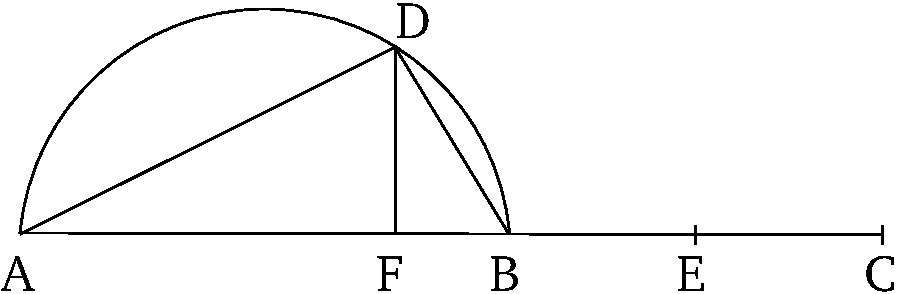
\includegraphics{Book10/fig034e.pdf}}

Let the two medial (straight-lines) $AB$ and $BC$, (which are) commensurable in square only, be laid out containing a medial (area), such
that the square on $AB$ is greater than (the square on) $BC$ by the
(square) on (some straight-line) incommensurable (in length) with ($AB$) [Prop.~10.32].  And let the semi-circle
$ADB$ be drawn on $AB$. And let the remainder (of the figure)
be generated similarly to the above (proposition).

And since $AF$ is incommensurable in length with $FB$ [Prop.~10.18], $AD$
is also incommensurable in square with $DB$ [Prop.~10.11]. And since the (square) on $AB$ is
medial, the sum of the (squares) on $AD$ and $DB$ (is) thus also
medial [Props.~3.31, 1.47]. And since the (rectangle
contained) by $AF$ and $FB$ is equal to the (square) on each of $BE$ and
$DF$, $BE$ is thus equal to $DF$. Thus, $BC$ (is) double $FD$. And
hence the (rectangle contained) by $AB$ and $BC$ is double the
(rectangle) contained by $AB$ and $FD$. And the (rectangle contained)
by $AB$ and $BC$ (is) medial. Thus, the (rectangle contained) by $AB$
and $FD$ (is) also medial. And it is equal to the (rectangle contained) 
by $AD$ and $DB$ [Prop.~10.32~lem.]. Thus, the
(rectangle contained) by $AD$ and $DB$ (is) also medial.
And since $AB$ is incommensurable in length with $BC$, and $CB$
(is) commensurable (in length) with $BE$, $AB$ (is) thus also incommensurable
in length with $BE$ [Prop.~10.13]. And hence the (square) on $AB$ is also incommensurable with the (rectangle contained) by $AB$ and $BE$ [Prop.~10.11]. But the (sum of the squares) on $AD$ and
$DB$ is equal to the (square) on $AB$ [Prop.~1.47].
And the (rectangle contained) by $AB$ and $FD$---that is to say, the (rectangle contained) by $AD$ and $DB$---is equal to the
(rectangle contained) by $AB$ and $BE$. Thus, the sum of the (squares) on
$AD$ and $DB$ is incommensurable with the (rectangle contained) by
$AD$ and $DB$.

Thus, two straight-lines, $AD$ and $DB$, (which are) incommensurable
in square, be found, making the sum of the (squares) on them
medial, and the (rectangle contained) by them medial, and, moreover, 
incommensurable  with the sum of the squares on them.$^\dag$
 (Which is) the
very thing it was required to show.}
\end{Parallel}
{\footnotesize\noindent$^\dag$ $AD$ and $DB$ have lengths
$k'^{1/4}\sqrt{[1+k/(1+k^2)^{1/2}]/2}$ and  $k'^{1/4}\sqrt{[1-k/(1+k^2)^{1/2}]/2}$ times that of $AB$, respectively, where $k$ and $k'$
are defined in the footnote to Prop.~10.32.}

%%%%%%
% Prop 10.36
%%%%%%
\pdfbookmark[1]{Proposition 10.36}{pdf10.36}
\begin{Parallel}{}{} 
\ParallelLText{
\begin{center}
{\large \ggn{36}.}
\end{center}\vspace*{-7pt}

\gr{Ἐὰν δύο <ρηταὶ δυνάμει μόνον σύμμετροι συντεθῶσιν, ἡ <όλη
>άλογόξ ἐστιν, καλείσθω δὲ ἐκ δύο ὀνομάτων.}\\

% Removed epsf size command
\centerline{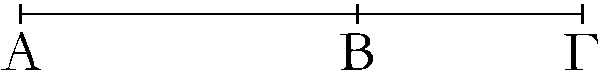
\includegraphics{Book10/fig036g.pdf}}

\gr{Συγκείσθωσαν γὰρ δύο <ρηταὶ δυνάμει μόνον σύμμετ\-ροι αἱ
ΑΒ, ΒΓ; λέγω, <ότι <όλη ἡ ΑΓ >άλογόξ ἐστιν.}

\gr{Ἐπεὶ γὰρ ἀσύμμετρόξ ἐστιν ἡ ΑΒ τῆ| ΒΓ μ\kern -.7pt  ήκει; δυνάμει
γὰρ μόνον εἰσὶ σύμμετροι; ὡξ δὲ ἡ ΑΒ πρὸξ τὴν ΒΓ, ο<ύτωξ
τὸ ὑπὸ τῶν ΑΒΓ πρὸξ τὸ ἀπὸ τῆξ ΒΓ, ἀσύμμετρον >άρα
ἐστὶ τὸ ὑπὸ τῶν ΑΒ, ΒΓ τῶ| ἀπὸ τῆξ ΒΓ. ἀλλὰ τῶ| μὲν
ὑπὸ τῶν ΑΒ, ΒΓ σύμμετρόν ἐστι τὸ δὶξ ὑπὸ τῶν ΑΒ, ΒΓ,
τῶ| δὲ ἀπὸ τῆξ ΒΓ σύμμετρά ἐστι τὰ ἀπὸ τῶν ΑΒ, ΒΓ;
αἱ γὰρ ΑΒ, ΒΓ <ρηταί εἰσι δυνάμει μόνον σύμμετροι; ἀσύμμετρον
>άρα ἐστὶ τὸ δὶξ ὑπὸ τῶν ΑΒ, ΒΓ τοῖξ
ἀπὸ τῶν ΑΒ, ΒΓ. καὶ συνθέντι τὸ δὶξ ὑπὸ τῶν ΑΒ, ΒΓ
μετὰ τῶν ἀπὸ τῶν ΑΒ, ΒΓ, τουτέστι τὸ ἀπὸ τῆξ ΑΓ,
ἀσύμμετρόν ἐστι τῶ| συγκειμένῳ ἐκ τῶν ἀπὸ τῶν ΑΒ, ΒΓ;
<ρητὸν δὲ τὸ συγκείμενον ἐκ τῶν ἀπὸ τῶν ΑΒ, ΒΓ;
>άλογον >άρα [ἐστὶ] τὸ ἀπὸ τῆξ ΑΓ; <ώστε καὶ ἡ ΑΓ >άλογόξ
ἐστιν, καλείσθω δὲ ἐκ δύο ὀνομάτων; <όπερ >έδει δεῖχαι.}}

\ParallelRText{
\begin{center}
{\large Proposition 36}
\end{center}

If two rational (straight-lines which are) commensurable
in square only are added together then the whole (straight-line) is irrational---let it
be called a binomial (straight-line).$^\dag$

% Removed epsf size command
\centerline{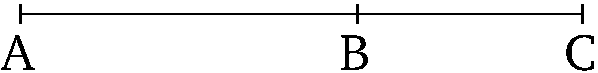
\includegraphics{Book10/fig036e.pdf}}

For let the two rational (straight-lines), $AB$ and $BC$, (which are)
commensurable in square only, be laid down together. I say that the
whole (straight-line), $AC$, is irrational.
For since $AB$ is incommensurable in length with $BC$---for they
are commensurable in square only---and as $AB$ (is) to $BC$, so
the (rectangle contained) by $ABC$ (is) to the (square) on $BC$, the (rectangle contained)
by $AB$ and $BC$ is thus incommensurable with the
(square) on $BC$ [Prop.~10.11]. But,
twice the (rectangle contained) by $AB$ and $BC$ is commensurable
with the (rectangle contained) by $AB$ and $BC$ [Prop.~10.6]. And (the sum of) the (squares) on
$AB$ and $BC$
 is commensurable with the (square) on $BC$---for the rational (straight-lines) $AB$ and $BC$ are commensurable in square only [Prop.~10.15].
Thus, twice the (rectangle contained) by $AB$ and $BC$ is incommensurable
with (the sum of) the (squares) on $AB$ and $BC$ [Prop.~10.13]. And, via composition, twice
the (rectangle contained) by $AB$ and $BC$, plus (the sum of) the (squares)
on $AB$ and $BC$---that is to say, the (square) on $AC$ [Prop.~2.4]---is incommensurable with the
sum of the (squares) on $AB$ and $BC$ [Prop.~10.16]. And the sum of the (squares) on $AB$ and $BC$ (is) rational. Thus, the (square) on $AC$ [is]
irrational [Def.~10.4]. Hence, $AC$
is also irrational [Def.~10.4]---let it be called
a binomial (straight-line).$^\ddag$  (Which is) the very thing it was required to show.}
\end{Parallel}
{\footnotesize\noindent$^\dag$ Literally, ``from two names".\\[0.5ex]
$^\ddag$ Thus, a binomial straight-line has a length
expressible as  $1 +k^{1/2}$ [or, more generally, $\rho\,(1+k^{1/2})$, where $\rho$ is rational---the same proviso applies to the definitions in the following propositions]. The binomial and the corresponding apotome, whose length is expressible as
$1-k^{1/2}$ (see Prop.~10.73), are
the positive roots of the quartic $x^4-2\,(1+k)\,x^2+ (1-k)^2 = 0$.}

%%%%%%
% Prop 10.37
%%%%%%
\pdfbookmark[1]{Proposition 10.37}{pdf10.37}
\begin{Parallel}{}{} 
\ParallelLText{
\begin{center}
{\large \ggn{37}.}
\end{center}\vspace*{-7pt}

\gr{Ἐὰν δύο μέσαι δυνάμει μόνον σύμμετροι συντεθῶσι <ρητὸν περιέθουσαι, ἡ <όλη >άλογόξ ἐστιν, καλείσθω δὲ ἐκ δύο μέσων
πρώτη.}\\

% Removed epsf size command
\centerline{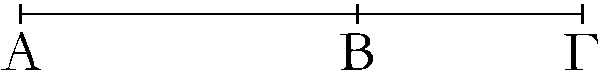
\includegraphics{Book10/fig036g.pdf}}

\gr{Συγκείσθωσαν γὰρ δύο μέσαι δυνάμει μόνον σύμμετ\-ροι αἱ ΑΒ, ΒΓ
<ρητὸν περιέθουσαι; λέγω, <ότι <όλη ἡ ΑΓ >άλογόξ ἐστιν.}

\gr{Ἐπεὶ γὰρ ἀσύμμετρόξ ἐστιν ἡ ΑΒ τῆ| ΒΓ μ\kern -.7pt  ήκει, καὶ τὰ ἀπὸ
τῶν ΑΒ, ΒΓ >άρα ἀσύμμετρά ἐστι τῶ| δὶξ ὑπὸ τῶν ΑΒ, ΒΓ;
καὶ συνθέντι τὰ ἀπὸ τῶν ΑΒ, ΒΓ μετὰ τοῦ δὶξ ὑπὸ τῶν ΑΒ, ΒΓ,
<όπερ ἐστὶ τὸ ἀπὸ τῆξ ΑΓ, ἀσύμμετρόν ἐστι τῶ| ὑπὸ τῶν
ΑΒ, ΒΓ.
<ρητὸν δὲ τὸ ὑπὸ τῶν ΑΒ, ΒΓ; ὑπόκεινται γὰρ αἱ ΑΒ, ΒΓ
<ρητὸν περιέθουσαι; >άλογον >άρα τὸ ἀπὸ τῆξ ΑΓ;
>άλογοξ >άρα ἡ ΑΓ, καλείσθω δὲ ἐκ δύο μέσων πρώτη; <όπερ
>έδει δεῖχαι.}}

\ParallelRText{
\begin{center}
{\large Proposition 37}
\end{center}

If two medial (straight-lines), commensurable in square only, which contain a rational (area), are added together then
the whole (straight-line) is irrational---let it be called a first bimedial (straight-line).$^\dag$

% Removed epsf size command
\centerline{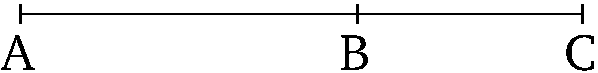
\includegraphics{Book10/fig036e.pdf}}

For let the  two medial (straight-lines), $AB$ and $BC$, 
commensurable in square only, (and) containing a rational (area), be laid down together. I say that the
whole (straight-line), $AC$, is irrational.

For since $AB$ is incommensurable in length with $BC$, (the sum of)
the (squares) on $AB$ and $BC$ is thus also incommensurable with twice
the (rectangle contained) by $AB$ and $BC$ [see previous proposition].
And, via composition, (the sum of) the (squares)  on $AB$ and $BC$,
plus twice the (rectangle contained) by $AB$ and $BC$---that is, 
the (square) on $AC$ [Prop.~2.4]---is incommensurable with the (rectangle contained) by $AB$ and $BC$
[Prop.~10.16]. And the (rectangle contained) by
$AB$ and $BC$ (is) rational---for $AB$ and $BC$ were assumed to
enclose a rational (area). Thus, the (square) on $AC$ (is) irrational. Thus, $AC$ (is) irrational [Def.~10.4]---let it be called
a first bimedial (straight-line).$^\ddag$
 (Which is) the very thing it was required to show.}
\end{Parallel}
{\footnotesize\noindent$^\dag$ Literally, ``first from two medials''.\\[0.5ex]
$^\ddag$ Thus, a first bimedial straight-line
has a length expressible as $k^{1/4}+k^{3/4}$. The first bimedial and the corresponding first apotome of a medial, whose length is expressible as
$k^{1/4}-k^{3/4}$ (see Prop.~10.74), are
the positive roots of the quartic $x^4-2\,\sqrt{k}\,(1+k)\,x^2+ k\,(1-k)^2 = 0$.}

%%%%%%
% Prop 10.38
%%%%%%
\pdfbookmark[1]{Proposition 10.38}{pdf10.38}
\begin{Parallel}{}{} 
\ParallelLText{
\begin{center}
{\large \ggn{38}.}
\end{center}\vspace*{-7pt}

\gr{Ἐὰν δύο μέσαι δυνάμει μόνον σύμμετροι συντεθῶσι μέσον περιέθουσαι, ἡ <όλη >άλογόξ ἐστιν, καλείσθω δὲ ἐκ δύο μέσων
δυετέρα.}\\

% Removed epsf size command
\centerline{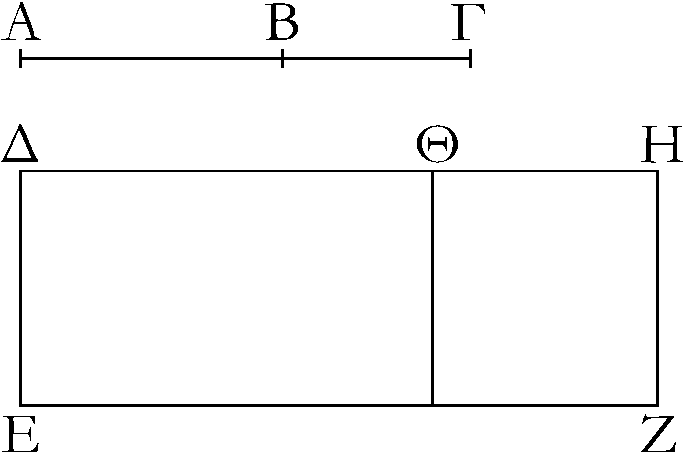
\includegraphics{Book10/fig038g.pdf}}

\gr{Συγκείσθωσαν γὰρ δύο μέσαι δυνάμει μόνον σύμμετ\-ροι αἱ ΑΒ, ΒΓ
μέσον περιέθουσαι; λέγω, <ότι >άλογόξ ἐστιν ἡ ΑΓ.}

\gr{Ἐκκείσθω γὰρ <ρητὴ ἡ ΔΕ, καὶ τῶ| ἀπὸ τῆξ ΑΓ >ίσον
παρὰ τὴν ΔΕ παραβεβλήσθω τὸ ΔΖ πλάτοξ ποιοῦν τὴν ΔΗ. καὶ
ἐπεὶ τὸ ἀπὸ τῆξ ΑΓ >ίσον ἐστὶ τοῖξ τε ἀπὸ τῶν ΑΒ, ΒΓ
καὶ τῶ| δὶξ ὑπὸ τῶν ΑΒ, ΒΓ, παραβεβλήσθω δὴ τοῖξ ἀπὸ τῶν
ΑΒ, ΒΓ παρὰ τὴν ΔΕ >ίσον τὸ ΕΘ; λοιπὸν >άρα τὸ ΘΖ >ίσον
ἐστὶ τῶ| δὶξ ὑπὸ τῶν ΑΒ, ΒΓ. καὶ ἐπεὶ μέση ἐστὶν ἑκατέρα
τῶν ΑΒ, ΒΓ, μέσα >άρα ἐστὶ καὶ τὰ ἀπὸ τῶν ΑΒ, ΒΓ. μέσον
δὲ ὑπόκειται καὶ τὸ δὶξ ὑπὸ τῶν ΑΒ, ΒΓ. καί ἐστι τοῖξ
μὲν ἀπὸ τῶν ΑΒ, ΒΓ >ίσον τὸ ΕΘ, τῶ| δὲ δὶξ ὑπὸ τῶν
ΑΒ, ΒΓ >ίσον τὸ ΖΘ; μέσον >άρα ἑκάτερον τῶν ΕΘ, ΘΖ. καὶ παρὰ
<ρητὴν τὴν ΔΕ παράκειται; <ρητὴ >άρα ἐστὶν ἑκατέρα τῶν
ΔΘ, ΘΗ καὶ ἀσύμμετροξ τῆ| ΔΕ μ\kern -.7pt  ήκει. ἐπεὶ ο>ῦν ἀσύμμετρόξ
ἐστιν ἡ ΑΒ τῆ| ΒΓ μ\kern -.7pt  ήκει, καί ἐστιν ὡξ ἡ ΑΒ πρὸξ τὴν ΒΓ, ο<ύτωξ
τὸ ἀπὸ τῆξ ΑΒ πρὸξ τὸ ὑπὸ τῶν ΑΒ, ΒΓ, ἀσύμμετρον >άρα ἐστὶ
τὸ ἀπὸ τῆξ ΑΒ τῶ| ὑπὸ τῶν ΑΒ, ΒΓ. ἀλλὰ τῶ| μὲν ἀπὸ τῆξ
ΑΒ σύμμετρόν ἐστι τὸ συγκείμενον ἐκ τῶν ἀπὸ τῶν ΑΒ, ΒΓ
τετραγώνων, τῶ| δὲ ὑπὸ τῶν ΑΒ, ΒΓ σύμμετρόν ἐστι τὸ δὶξ
ὑπὸ τῶν ΑΒ, ΒΓ. ἀσύμμετρον >άρα ἐστὶ τὸ συγκείμενον
ἐκ τῶν ἀπὸ τῶν ΑΒ, ΒΓ τῶ| δὶξ ὑπὸ τῶν ΑΒ, ΒΓ. ἀλλὰ
τοῖξ μὲν ἀπὸ τῶν ΑΒ, ΒΓ >ίσον ἐστὶ τὸ ΕΘ, τῶ| δὲ δὶξ ὑπὸ
τῶν ΑΒ, ΒΓ >ίσον
ἐστὶ τὸ ΘΖ. ἀσύμμετρον >άρα ἐστὶ τὸ ΕΘ τῶ| ΘΖ; <ώστε καὶ ἡ ΔΘ
τῆ| ΘΗ ἐστιν ἀσύμμετροξ μ\kern -.5pt  ήκει. αἱ ΔΘ, ΘΗ >άρα <ρηταί εἰσι
δυνάμει μόνον σύμμετροι. <ώστε ἡ ΔΗ >άλογόξ ἐστιν. <ρητὴ δὲ ἡ ΔΕ; τὸ δὲ ὑπὸ ἀλόγου καὶ <ρητῆξ περιεχόμενον ὀρθογώνιον
>άλογόν ἐστιν; >άλογον >άρα ἐστὶ τὸ ΔΖ θωρίον, καὶ ἡ δυναμένη
[α\kern -.3pt  ὐτὸ] >άλογόξ ἐστιν. δύναται δὲ τὸ ΔΖ ἡ ΑΓ; >άλογοξ >άρα
ἐστὶν ἡ ΑΓ, καλείσθω δὲ ἐκ δύο μέσων δευτέρα. <όπερ
>έδει δεῖχαι.}}

\ParallelRText{
\begin{center}
{\large Proposition 38}
\end{center}
If two medial (straight-lines), commensurable in
square only, which contain a medial (area), are added together then the
whole (straight-line) is irrational---let it be called a second bimedial
(straight-line).

% Removed epsf size command
\centerline{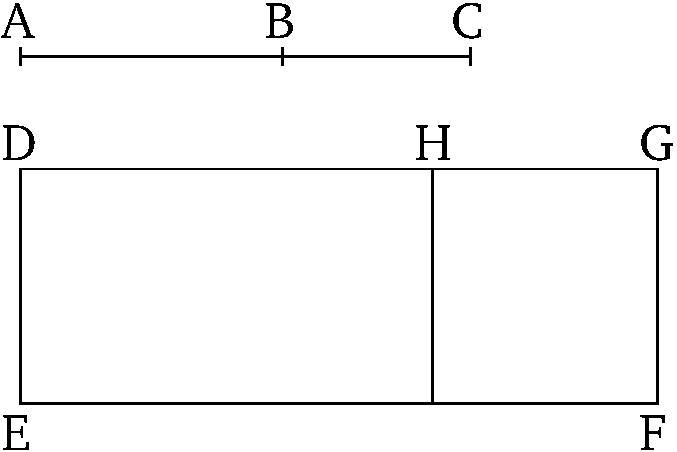
\includegraphics{Book10/fig038e.pdf}}

For let the  two medial (straight-lines), $AB$ and $BC$, 
commensurable in square only, (and) containing a medial (area), be laid down together [Prop.~10.28]. I say that $AC$ is irrational.

For let the rational (straight-line) $DE$ be laid down, and let (the rectangle) $DF$, equal
to the (square) on $AC$, be applied to $DE$, making $DG$ as breadth
[Prop.~1.44]. And since the
(square) on $AC$ is equal to (the sum of) the (squares) on $AB$ and $BC$,
plus twice the (rectangle contained) by $AB$ and $BC$ [Prop.~2.4], so let (the rectangle) $EH$, equal to
(the sum of) the squares on $AB$ and $BC$, be applied
to $DE$. The remainder $HF$ is thus equal to twice the (rectangle contained)
by $AB$ and $BC$. And since $AB$ and $BC$ are each medial, (the
sum of) the squares on $AB$ and $BC$ is thus also medial.$^\ddag$ And twice the (rectangle contained) by $AB$ and $BC$ was also assumed (to be) medial.
And $EH$ is equal to (the sum of) the squares on $AB$ and $BC$, and
$FH$ (is) equal to twice the (rectangle contained) by $AB$ and $BC$. 
Thus, $EH$ and $HF$ (are) each medial. And they were applied to the
rational (straight-line) $DE$. Thus, $DH$ and $HG$ are
each rational, and incommensurable in length with $DE$ [Prop.~10.22]. Therefore, since $AB$ is incommensurable in length with $BC$, and as $AB$ is to $BC$, so the
(square) on $AB$ (is) to the (rectangle contained) by $AB$ and $BC$ [Prop.~10.21~lem.], the (square) on $AB$
is thus incommensurable with the (rectangle contained) by $AB$ and $BC$
[Prop.~10.11]. But, the sum of the squares on $AB$ and $BC$ is commensurable with the (square) on $AB$ [Prop.~10.15], and twice the (rectangle contained)
by $AB$ and $BC$ is commensurable with the (rectangle contained) by $AB$ and $BC$ [Prop.~10.6]. Thus, the sum of
the (squares) on $AB$ and $BC$ is incommensurable with twice the (rectangle
contained) by $AB$ and $BC$ [Prop.~10.13].
But, $EH$ is equal to (the sum of) the squares on $AB$ and $BC$,
and $HF$ is equal to twice the (rectangle) contained by $AB$ and $BC$. Thus, $EH$ is incommensurable with $HF$. Hence, $DH$ is also
incommensurable in length with $HG$ [Props.~6.1, 10.11]. Thus, $DH$ and 
$HG$ are rational (straight-lines which are) commensurable in square only.
Hence, $DG$ is irrational [Prop.~10.36].
And  $DE$ (is) rational. And the rectangle contained by irrational and
rational (straight-lines) is irrational [Prop.~10.20].
The area $DF$ is thus irrational, and (so) the square-root [of it] is irrational
[Def.~10.4]. And  $AC$ is the square-root of $DF$. $AC$ is thus irrational---let it be called a second bimedial (straight-line).$^\S$ (Which is) the very thing it was required to show.}
\end{Parallel}
{\footnotesize\noindent$^\dag$ Literally, 
``second from two medials''.\\[0.5ex]
$^\ddag$ Since, by hypothesis, the squares on $AB$ and $BC$ are commensurable---see Props.~10.15, 10.23.\\[0.5ex]
$^\S$ Thus, a second bimedial straight-line
has a length expressible as $k^{1/4}+k'^{1/2}/k^{1/4}$. The second bimedial and the corresponding second apotome of a medial, whose length is expressible as
$k^{1/4}-k'^{1/2}/k^{1/4}$ (see Prop.~10.75), are
the positive roots of the quartic $x^4-2\,[(k+k')/\sqrt{k}\,]\,x^2+ [(k-k')^2/k] = 0$.}

%%%%%%
% Prop 10.39
%%%%%%
\pdfbookmark[1]{Proposition 10.39}{pdf10.39}
\begin{Parallel}{}{} 
\ParallelLText{
\begin{center}
{\large \ggn{39}.}
\end{center}\vspace*{-7pt}

\gr{Ἐὰν δύο εὐθεῖαι δυνάμει ἀσύμμετροι συντεθῶσι ποιοῦσ\-αι τὸ
μὲν συγκείμενον ἐκ τῶν ἀπ> α\kern -.7pt  ὐτῶν τετραγώνων <ρητόν, τὸ
δ> ὑπ> α\kern -.7pt  ὐτῶν μέσον, ἡ <όλη εὐθεῖα >άλογόξ ἐστιν, καλείσθω
δὲ μείζων.}\\

% Removed epsf size command
\centerline{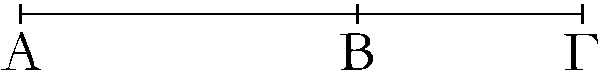
\includegraphics{Book10/fig036g.pdf}}

\gr{Συγκείσθωσαν γὰρ δύο εὐθεῖαι δυνάμει ἀσύμμετροι αἱ ΑΒ, ΒΓ
ποιοῦσαι τὰ προκείμενα; λέγω, <ότι >άλογόξ ἐστιν ἡ ΑΓ.}

\gr{Ἐπεὶ γὰρ τὸ ὑπὸ τῶν ΑΒ, ΒΓ μέσον ἐστίν, καὶ τὸ δὶξ [>άρα]
ὑπὸ τῶν ΑΒ, ΒΓ μέσον ἐστίν. τὸ δὲ συγκείμενον ἐκ τῶν
ἀπὸ τῶν ΑΒ, ΒΓ <ρητόν; ἀσύμμετρον >άρα ἐστὶ τὸ δὶξ ὑπὸ
τῶν ΑΒ, ΒΓ τῶ| συγκειμένῳ ἐκ τῶν ἀπὸ τῶν ΑΒ, ΒΓ;
 <ώστε καὶ τὰ ἀπὸ τῶν ΑΒ, ΒΓ μετὰ τοῦ δὶξ ὑπὸ
τῶν ΑΒ, ΒΓ, <όπερ ἐστὶ τὸ ἀπὸ τῆξ ΑΓ, ἀσύμμετρόν ἐστι
τῶ| συγκειμένῳ ἐκ τῶν ἀπὸ τῶν ΑΒ, ΒΓ [<ρητὸν δὲ τὸ συγμείμενον ἐκ τῶν ἀπὸ τῶν ΑΒ, ΒΓ]; >άλογον >άρα ἐστὶ
τὸ ἀπὸ τῆξ ΑΓ. <ώστε καὶ ἡ ΑΓ >άλογόξ ἐστιν, καλείσθω
δὲ μείζων. <όπερ >έδει δεῖχαι.}}

\ParallelRText{
\begin{center}
{\large Proposition 39}
\end{center}

If two straight-lines (which are) incommensurable
in square, making the sum of the squares on them
rational, and the (rectangle contained) by them medial,  are added together then the whole
straight-line is irrational---let it be called a major (straight-line).

% Removed epsf size command
\centerline{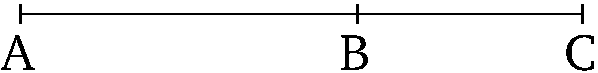
\includegraphics{Book10/fig036e.pdf}}

For let the two straight-lines, $AB$ and $BC$,  incommensurable
in square, and fulfilling  the  prescribed (conditions), be laid down together [Prop.~10.33]. I say that $AC$ is irrational.

For since the (rectangle contained) by $AB$ and $BC$ is medial, twice
the (rectangle contained) by $AB$ and $BC$ is [thus] also medial [Props.~10.6, 10.23~corr.].
And the sum of the (squares) on $AB$ and $BC$ (is) rational. Thus, twice
the (rectangle contained) by $AB$ and $BC$ is incommensurable with the
sum of the (squares) on $AB$ and $BC$ [Def.~10.4].
Hence, (the sum of) the squares on $AB$ and $BC$, plus twice the
(rectangle contained) by $AB$ and $BC$---that is, the (square) on $AC$ [Prop.~2.4]---is also
incommensurable with the sum of the (squares) on $AB$ and $BC$
[Prop.~10.16] [and the
sum of the (squares) on $AB$ and $BC$ (is) rational]. Thus, the (square) on $AC$ is irrational. Hence, $AC$ is also irrational [Def.~10.4]---let it be called a major (straight-line).$^\dag$ (Which is) the
very thing it was required to show.}
\end{Parallel}
{\footnotesize\noindent$^\dag$ Thus, a major straight-line
has a length expressible as $\sqrt{[1+k/(1+k^2)^{1/2}]/2} + \sqrt{[1-k/(1+k^2)^{1/2}]/2}$. The major and the corresponding minor, whose length is expressible as $\sqrt{[1+k/(1+k^2)^{1/2}]/2} - \sqrt{[1-k/(1+k^2)^{1/2}]/2}$ (see Prop.~10.76), are
the positive roots of the quartic $x^4-2\,x^2+ k^2/(1+k^2) = 0$.}

%%%%%%
% Prop 10.40
%%%%%%
\pdfbookmark[1]{Proposition 10.40}{pdf10.40}
\begin{Parallel}{}{} 
\ParallelLText{
\begin{center}
{\large\ggn{40}.}
\end{center}\vspace*{-7pt}

\gr{Ἐὰν δύο εὐθεῖαι δυνάμει ἀσύμμετροι συντεθῶσι ποιοῦσ\-αι τὸ μὲν
συγκείμενον ἐκ τῶν ἀπ> α\kern -.7pt  ὐτῶν τετραγώνων μέσον, τὸ δ> ὑπ>
α\kern -.7pt  ὐτῶν <ρητόν, ἡ <όλη εὐθεῖα >άλογόξ ἐστιν, καλείσθω δὲ
<ρητὸν καὶ μέσον δυναμένη.}\\~\\

% Removed epsf size command
\centerline{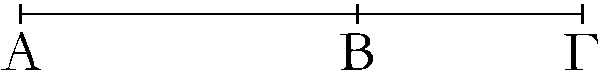
\includegraphics{Book10/fig036g.pdf}}

\gr{Συγκείσθωσαν γὰρ δύο εὐθεῖαι δυνάμει ἀσύμμετροι αἱ ΑΒ, ΒΓ
ποιοῦσαι τὰ προκείμενα; λέγω, <ότι >άλογόξ ἐστιν ἡ ΑΓ.}

\gr{Ἐπεὶ γὰρ τὸ συγκείμενον ἐκ τῶν ἀπὸ τῶν ΑΒ, ΒΓ μέσον
ἐστίν, τὸ δὲ δὶξ ὑπὸ τῶν ΑΒ, ΒΓ <ρητόν, ἀσύμμετρον
>άρα ἐστὶ τὸ συγκείμενον ἐκ τῶν ἀπὸ τῶν ΑΒ, ΒΓ τῶ| δὶξ
ὑπὸ τῶν ΑΒ, ΒΓ; <ώστε καὶ τὸ ἁπὸ τῆξ ΑΓ ἀσύμμετρόν ἐστι
τῶ| δὶξ ὑπὸ τῶν ΑΒ, ΒΓ. <ρητὸν δὲ τὸ δὶξ ὑπὸ τῶν ΑΒ, ΒΓ;
>άλογον >άρα τὸ ἀπὸ τῆξ ΑΓ. >άλογοξ >άρα ἡ ΑΓ, καλείσθω δὲ <ρητὸν
καὶ μέσον δυναμένη. <όπερ >έδει δεῖχαι.}}

\ParallelRText{
\begin{center}
{\large Proposition 40}
\end{center}

If two straight-lines (which are) incommensurable
in square, making the sum of the squares on them medial, 
and the (rectangle contained) by them rational, are added together then the whole straight-line
is irrational---let it be called the square-root of a rational plus a medial (area).

% Removed epsf size command
\centerline{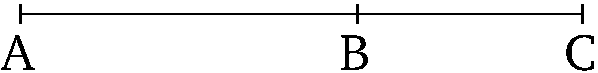
\includegraphics{Book10/fig036e.pdf}}

For let the two straight-lines, $AB$ and $BC$, incommensurable
in square, (and) fulfilling the prescribed (conditions), be laid down together [Prop.~10.34]. I say that $AC$ is irrational.

For since the sum of the (squares) on $AB$ and $BC$ is medial,
and twice the (rectangle contained) by $AB$ and $BC$ (is) rational, 
the sum of the (squares) on $AB$ and $BC$ is thus incommensurable
with twice the (rectangle contained) by $AB$ and $BC$. Hence, the (square)
on $AC$ is also incommensurable with twice the (rectangle contained)
by $AB$ and $BC$ [Prop.~10.16]. And twice the
(rectangle contained) by $AB$ and $BC$ (is) rational. The (square) on
$AC$ (is) thus irrational. Thus, $AC$ (is) irrational [Def.~10.4]---let it be called
the square-root of a rational plus a medial (area).$^\dag$
(Which is) the very thing it
was required to show.}
\end{Parallel}
{\footnotesize\noindent$^\dag$ Thus, the square-root
of a rational plus a medial (area)
has a length expressible as $\sqrt{[(1+k^2)^{1/2}+k]/[2\,(1+k^2)]} +\sqrt{[(1+k^2)^{1/2}-k]/[2\,(1+k^2)]}$. This  and the corresponding irrational with a minus sign, whose length is expressible as $\sqrt{[(1+k^2)^{1/2}+k]/[2\,(1+k^2)]} -\sqrt{[(1+k^2)^{1/2}-k]/[2\,(1+k^2)]}$
 (see Prop.~10.77), are the positive roots of the quartic $x^4-(2/\sqrt{1+k^2})\,x^2+ k^2/(1+k^2)^2 = 0$.} 
 
%%%%%%
% Prop 10.41
%%%%%%
\pdfbookmark[1]{Proposition 10.41}{pdf10.41}
\begin{Parallel}{}{} 
\ParallelLText{
\begin{center}
{\large\ggn{41}.}
\end{center}\vspace*{-7pt}

\gr{Ἐὰν δύο εὐθεῖαι δυνάμει ἀσύμμετροι συντεθῶσι ποιοῦσ\-αι τό
τε συγκείμενον ἐκ τῶν ἀπ> α\kern -.7pt  ὐτῶν τετραγώνων μέσον καὶ τὸ
ὑπ> α\kern -.7pt  ὐτῶν μέσον καὶ >έτι ἀσύμμετρον τῶ| συγκειμένῳ
ἐκ τῶν ἀπ> α\kern -.5pt  ὐτῶν τετραγώνων, ἡ <όλη εὐθεῖα >άλογόξ
ἐστιν, καλείσθω δὲ δύο μέσα δυναμένη.}\\

% Removed epsf size command
\centerline{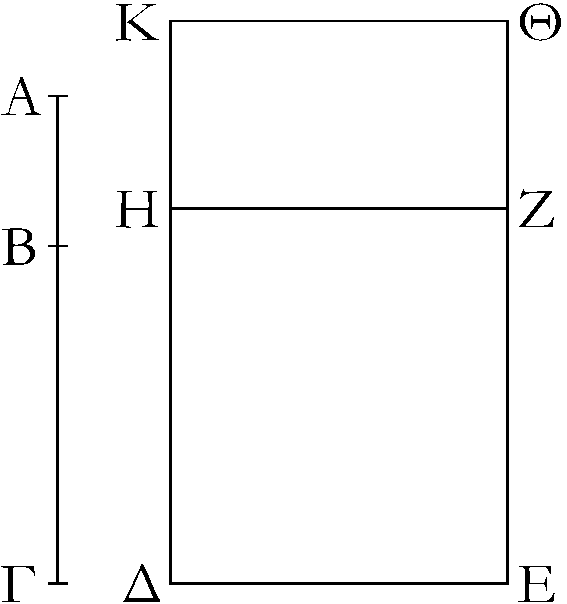
\includegraphics{Book10/fig041g.pdf}}

\gr{Συγκείσθωσαν γὰρ δύο εὐθεῖαι δυνάμει ἀσύμμετροι
αἱ ΑΒ, ΒΓ ποιοῦσαι τὰ προκείμενα; λέγω, <ότι ἡ ΑΓ >άλογόξ
ἐστιν.}

\gr{Ἐκκείσθω <ρητὴ ἡ ΔΕ, καὶ παραβεβλήσθω παρὰ τὴν ΔΕ τοῖξ μὲν ἀπὸ
τῶν ΑΒ, ΒΓ >ίσον τὸ ΔΖ, τῶ| δὲ δὶξ ὑπὸ τῶν ΑΒ, ΒΓ >ίσον
τὸ ΗΘ; <όλον >άρα τὸ ΔΘ >ίσον ἐστὶ τῶ| ἀπὸ τῆξ ΑΓ τετραγώνῳ.
καὶ ἐπεὶ μέσον ἐστὶ τὸ συγκείμενον ἐκ τῶν ἀπὸ τῶν
ΑΒ, ΒΓ, καί ἐστιν >ίσον τῶ| ΔΖ, μέσον >άρα ἐστὶ καὶ τὸ ΔΖ.
καὶ παρὰ <ρητὴν τὴν ΔΕ παράκειται; <ρητὴ >άρα ἐστὶν ἡ
ΔΗ καὶ ἀσύμμετροξ τῆ| ΔΕ μ\kern -.7pt  ήκει. διὰ τὰ α\kern -.7pt  ὐτὰ δὴ
καὶ ἡ ΗΚ <ρητή ἐστι καὶ ἀσύμμετροξ τῆ| ΗΖ, τουτέστι τῆ| ΔΕ, μ\kern -.5pt  ήκει.
καὶ ἐπεὶ ἀσύμμετρά ἐστι τὰ ἀπὸ τῶν ΑΒ, ΒΓ τῶ| δὶξ
ὑπὸ τῶν ΑΒ, ΒΓ, ἀσύμμετρόν ἐστι τὸ ΔΖ τῶ| ΗΘ; <ώστε καὶ ἡ
ΔΗ τῆ| ΗΚ ἀσύμμετρόξ ἐστιν. καὶ εἰσι <ρηταί; αἱ ΔΗ, ΗΚ
>άρα <ρηταί εἰσι δυνάμει μόνον σύμμετροι;
>άλογοξ >άρα ἐστὶν ἡ ΔΚ ἡ καλουμένη ἐκ δύο ὀνομάτων.
<ρητὴ δὲ ἡ ΔΕ; >άλογον >άρα ἐστὶ τὸ ΔΘ καὶ ἡ δυναμένη
α\kern -.3pt  ὐτὸ >άλογόξ ἐστιν. δύναται δὲ τὸ ΘΔ ἡ ΑΓ; >άλογοξ >άρα
ἐστὶν ἡ ΑΓ, καλείσθω δὲ δύο μέσα δυναμένη. <όπερ >έδει δεῖχαι.}}

\ParallelRText{
\begin{center}
{\large Proposition 41}
\end{center}

If two straight-lines (which are) incommensurable
in square, making the sum of the squares
on them medial, and the (rectangle contained) by them medial, and,
moreover, incommensurable with the sum of the squares on them, are added together then
the whole straight-line is irrational---let it be called the square-root
of (the sum of) two medial (areas).

% Removed epsf size command
\centerline{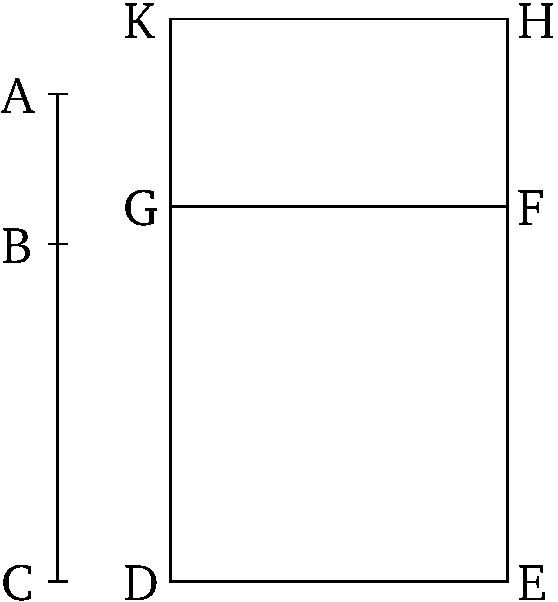
\includegraphics{Book10/fig041e.pdf}}

For let the two straight-lines, $AB$ and $BC$,  incommensurable
in square,  (and) fulfilling the prescribed (conditions), be laid down together
[Prop.~10.35]. I say that $AC$ is irrational.

Let the rational (straight-line) $DE$ be laid out, and let (the rectangle) $DF$,
equal to (the sum of) the (squares) on $AB$ and $BC$, and (the rectangle) $GH$, equal to twice the (rectangle contained) by
$AB$ and $BC$, be applied
to $DE$. Thus, the whole of $DH$ is equal to the square on $AC$
[Prop.~2.4]. And since the sum of the (squares)
on $AB$ and $BC$ is medial, and is equal to $DF$, $DF$ is thus also
medial. And it is applied to the rational (straight-line) $DE$. 
Thus, $DG$ is rational, and incommensurable in length with $DE$ [Prop.~10.22]. So, for the same (reasons), $GK$
is also rational, and incommensurable in length with $GF$---that is
to say, $DE$. And since (the sum of) the (squares) on $AB$ and $BC$
is incommensurable with twice the (rectangle contained) by $AB$ and
$BC$, $DF$ is incommensurable with $GH$.
Hence, $DG$ is also incommensurable (in length)
with $GK$ [Props.~6.1, 10.11]. And they are rational. Thus, $DG$ and
$GK$ are rational (straight-lines which are) commensurable in square only. Thus, $DK$ is irrational, and that (straight-line which is) called binomial 
[Prop.~10.36]. And $DE$ (is) rational.
Thus, $DH$ is irrational, and its square-root is irrational [Def.~10.4]. And $AC$ (is) the square-root of $HD$. Thus,
$AC$ is irrational---let it be called the square-root of (the sum of) two medial
(areas).$^\dag$ (Which is) the very thing it was required to show.}
\end{Parallel}
{\footnotesize\noindent$^\dag$ Thus, the square-root
of (the sum of) two medial (areas)
has a length expressible as $k'^{1/4}\left(\sqrt{[1+k/(1+k^2)^{1/2}]/2}
+\sqrt{[1-k/(1+k^2)^{1/2}]/2}\right)$. This  and the corresponding irrational with a minus sign, whose length is expressible as $k'^{1/4}\left(\sqrt{[1+k/(1+k^2)^{1/2}]/2}
-\sqrt{[1-k/(1+k^2)^{1/2}]/2}\right)$
 (see Prop.~10.78), are
the positive roots of the quartic $x^4-2\,k'^{1/2}\,x^2+ k'\, k^2/(1+k^2)= 0$.} 

%%%%%%
% Prop 10.41a
%%%%%%
\begin{Parallel}{}{} 
\ParallelLText{
\begin{center}
{\large \gr{Λῆμμα}.}
\end{center}\vspace*{-7pt}

\gr{<'Οτι δὲ αἱ εἰρημέναι >άλογοι μοναθῶξ διαιροῦνται εἰξ
τὰξ εὐθείαξ, ἐχ <ῶν σύγκεινται ποιουσῶν τὰ προκείμενα
ε>ίδη, δείχομεν >ήδη προεκθέμενοι λημμάτιον τοιοῦτον;}\\

% Removed epsf size command
\centerline{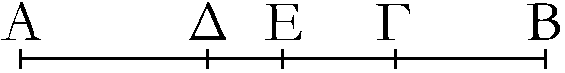
\includegraphics{Book10/fig041ag.pdf}}

\gr{Ἐκκείσθω εὐθεῖα ἡ ΑΒ καὶ τετμ\kern -.7pt  ήσθω ἡ <όλη εἰξ >άνισα
καθ> ἑκάτερον τῶν Γ, Δ, ὑποκείσθω δὲ μείζων ἡ ΑΓ τῆξ ΔΒ;
λέγω, <ότι τὰ ἀπὸ τῶν ΑΓ, ΓΒ μείζονά ἐστι τῶν ἀπὸ
τῶν ΑΔ, ΔΒ.}

\gr{Τετμ\kern -.7pt  ήσθω γὰρ ἡ ΑΒ δίθα κατὰ τὸ Ε. καὶ ἐπεὶ μείζων ἐστὶν
ἡ ΑΓ τῆξ ΔΒ, κοινὴ ἀφῃρήσθω ἡ ΔΓ; λοιπὴ >άρα ἡ ΑΔ λοιπῆξ
τῆξ ΓΒ μείζων ἐστίν. >ίση δὲ ἡ ΑΕ τῆ| ΕΒ; ἐλάττων
>άρα ἡ ΔΕ τῆξ ΕΓ; τὰ Γ, Δ >άρα σημεῖα οὐκ >ίσον
ἀπέθουσι τῆξ διθοτομίαξ. καὶ ἐπεὶ τὸ ὑπὸ τῶν ΑΓ, ΓΒ
μετὰ τοῦ ἀπὸ τῆξ ΕΓ >ίσον ἐστὶ τῶ| ἀπὸ τῆξ ΕΒ, ἀλλὰ
μ\kern -.7pt  ὴν καὶ τὸ ὑπὸ τῶν ΑΔ, ΔΒ μετὰ τοῦ ἀπὸ ΔΕ >ίσον
ἐστὶ τῶ| ἀπὸ τῆξ ΕΒ, τὸ >άρα ὑπὸ τῶν
ΑΓ, ΓΒ μετὰ τοῦ ἀπὸ τῆξ ΕΓ >ίσον ἐστὶ τῶ| ὑπὸ τῶν ΑΔ, ΔΒ μετὰ τοῦ ἀπὸ τῆξ ΔΕ; <ῶν τὸ ἀπὸ τῆξ ΔΕ
>έλασσόν ἐστι τοῦ ἀπὸ τῆξ ΕΓ; καὶ λοιπὸν >άρα τὸ ὑπὸ
τῶν ΑΓ, ΓΒ >έλασσόν ἐστι τοῦ ὑπὸ τῶν ΑΔ, ΔΒ. <ώστε
καὶ τὸ δὶξ ὑπὸ τῶν ΑΓ, ΓΒ >έλασσόν ἐστι τοῦ δὶξ ὑπὸ τῶν
ΑΔ, ΔΒ. καὶ λοιπὸν >άρα τὸ συγκείμενον ἐκ τῶν ἀπὸ τῶν
ΑΓ, ΓΒ μεῖζόν ἐστι τοῦ συγκειμένου ἐκ τῶν ἀπὸ τῶν
ΑΔ, ΔΒ. <όπερ >έδει δεῖχαι.}}

\ParallelRText{
\begin{center}
{\large Lemma}
\end{center}

We will now demonstrate that the aforementioned irrational (straight-lines)
 are uniquely divided into the straight-lines  of which they are the sum,
 and which produce the prescribed types, 
 (after) setting forth the following
 lemma.
 
 % Removed epsf size command
\centerline{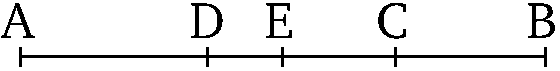
\includegraphics{Book10/fig041ae.pdf}}
 
 Let the straight-line $AB$ be laid out, and let the whole (straight-line) be cut
 into unequal parts at each of the (points) $C$ and $D$. And let $AC$ be assumed (to be) greater than $DB$. I say that (the sum of) the (squares) on
 $AC$ and $CB$ is greater than (the sum of) the (squares) on $AD$ and $DB$.
 
 For let $AB$ be cut in half at $E$. And since $AC$ is greater than
 $DB$, let $DC$ be subtracted from both. Thus, the remainder
 $AD$ is greater than the remainder $CB$. And $AE$ (is) equal to $EB$.
 Thus, $DE$ (is) less than $EC$. Thus, points $C$ and $D$ are not
 equally far from the point of bisection. And since the (rectangle
 contained) by $AC$ and $CB$, plus the (square) on $EC$,
 is equal to the (square) on $EB$ [Prop.~2.5], 
 but, moreover, the (rectangle contained) by $AD$ and $DB$, plus the
 (square) on $DE$, is also equal to the (square) on $EB$ [Prop.~2.5], the (rectangle contained) by $AC$ and
 $CB$, plus the (square) on $EC$, is thus equal to the (rectangle contained)
 by $AD$ and $DB$, plus the (square) on $DE$. And, of these, the
 (square) on $DE$ is less than the (square) on $EC$. And, thus, the remaining
 (rectangle contained) by $AC$ and $CB$ is  less than
 the (rectangle contained) by $AD$ and $DB$. And, hence, twice
 the (rectangle contained) by $AC$ and $CB$ is less than twice the
 (rectangle contained) by $AD$ and $DB$. And thus the remaining
 sum of the (squares) on $AC$ and $CB$ is greater than the sum of the
 (squares) on $AD$ and $DB$.$^\dag$  (Which is) the very thing it was required to show.}
\end{Parallel}
{\footnotesize\noindent$^\dag$ Since, $AC^{\,2}+CB^{\,2}+2\,AC\,CB=
 AD^{\,2}+DB^{\,2}
+2\,AD\,DB = AB^{\,2}$.} 

%%%%%%
% Prop 10.42
%%%%%%
\pdfbookmark[1]{Proposition 10.42}{pdf10.42}
\begin{Parallel}{}{} 
\ParallelLText{
\begin{center}
{\large \ggn{42}.}
\end{center}\vspace*{-7pt}

\gr{Ἡ ἐκ δύο ὀνομάτων κατὰ <ὲν μόνον σημεῖον διαιρεῖται εἰξ
τὰ ὀνόματα.}

% Removed epsf size command
\centerline{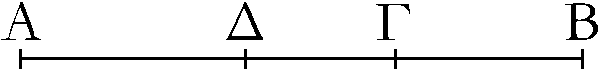
\includegraphics{Book10/fig042g.pdf}}

\gr{>'Εστω ἐκ δύο ὀνομάτων ἡ ΑΒ διῃρημένη εἰξ τὰ ὀνόματα
κατὰ τὸ Γ; αἱ ΑΓ, ΓΒ >άρα <ρηταί εἰσι δυνάμει μόνον σύμμετροι.
λέγω, <ότι ἡ ΑΒ κατ> >άλλο σημεῖον οὐ διαιρεῖται εἰξ δύο
<ρητὰξ δυνάμει μόνον συμμέτρουξ.}

\gr{Εἰ γὰρ δυνατόν, διῃρήσθω καὶ κατὰ τὸ Δ, <ώστε καὶ τὰξ ΑΔ,
ΔΒ <ρητὰξ ε>ῖναι δυνάμει μόνον συμμέτρουξ. φανερὸν δή,
<ότι ἡ ΑΓ τῆ| ΔΒ οὐκ >έστιν ἡ α\kern -.7pt  ὐτή. εἰ γὰρ δυνατόν,
>έστω. >έσται δὴ καὶ ἡ ΑΔ τῆ| ΓΒ ἡ α\kern -.7pt  ὐτή; καὶ >έσται
ὡξ ἡ ΑΓ πρὸξ τὴν ΓΒ, ο<ύτωξ ἡ ΒΔ πρὸξ τὴν ΔΑ,
καὶ >έσται ἡ ΑΒ κατὰ τὸ α\kern -.5pt  ὐτὸ τῆ| κατὰ τὸ Γ διαιρέσει διαιρεθεῖσα
καὶ κατὰ τὸ Δ; <όπερ οὐθ ὑπόκειται. οὐκ >άρα ἡ ΑΓ τῆ|
ΔΒ ἐστιν ἡ α\kern -.3pt  ὐτή. διὰ δὴ τοῦτο καὶ τὰ Γ, Δ σημεῖα
οὐκ >ίσον ἀπέθουσι τῆξ διθοτομίαξ. <ῶ| >άρα διαφέρει τὰ
ἀπὸ τῶν ΑΓ, ΓΒ τῶν ἀπὸ τῶν ΑΔ, ΔΒ, τούτῳ διαφέρει καὶ
τὸ δὶξ ὑπὸ τῶν ΑΔ, ΔΒ τοῦ δὶξ ὑπὸ τῶν ΑΓ, ΓΒ
διὰ τὸ καὶ τὰ ἀπὸ τῶν ΑΓ, ΓΒ μετὰ τοῦ δὶξ ὑπὸ τῶν
ΑΓ, ΓΒ καὶ τὰ ἀπὸ τῶν ΑΔ, ΔΒ μετὰ τοῦ δὶξ ὑπὸ τῶν
ΑΔ, ΔΒ >ίσα ε>ῖναι τῶ| ἀπὸ τῆξ ΑΒ. ἀλλὰ τὰ ἀπὸ
τῶν ΑΓ, ΓΒ τῶν ἀπὸ τῶν ΑΔ, ΔΒ διαφέρει <ρητῶ|;
<ρητὰ γὰρ ἀμφότερα; καὶ τὸ δὶξ >άρα ὑπὸ τῶν ΑΔ, ΔΒ
τοῦ δὶξ ὑπὸ τῶν ΑΓ, ΓΒ διαφέρει <ρητῶ| μέσα
>όντα; <όπερ >άτοπον; μέσον γὰρ μέσου οὐθ ὑπερέθει
<ρητῶ|.}

\gr{Οὐθ >άρα ἡ ἐκ δύο ὀνομάτων κατ> >άλλο καὶ >άλλο
σημεῖον διαιρεῖται; καθ> <ὲν >άρα μόνον; <όπερ
>έδει δεῖχαι.}}

\ParallelRText{
\begin{center}
{\large Proposition 42}
\end{center}
A binomial (straight-line) can be divided into
its (component) terms at one
point only.$^\dag$

% Removed epsf size command
\centerline{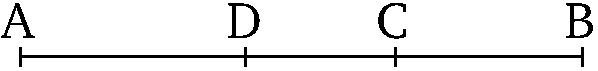
\includegraphics{Book10/fig042e.pdf}}

Let $AB$ be a binomial (straight-line) which has been divided into its
(component) terms at $C$. $AC$ and $CB$ are thus
rational (straight-lines which are) commensurable in square only [Prop.~10.36]. I say that $AB$ cannot be divided
at another point
into two rational (straight-lines which are) commensurable in square only.

For, if possible, let it also be divided at $D$, such that $AD$ and
$DB$ are also rational (straight-lines which are) commensurable in
square only. So, (it is) clear that $AC$ is not the same as $DB$.
For, if possible, let it be (the same). So, $AD$ will also be the same
as $CB$. And as $AC$ will be to $CB$, so $BD$ (will be) to $DA$.
And $AB$ will (thus) also be divided at $D$ in the same (manner) as the division at $C$. The very opposite was assumed. Thus, $AC$ is not the
same as $DB$. So, on account of this,  points $C$ and $D$ are
not equally far from the point of bisection. Thus, by whatever (amount the sum of) the (squares) on $AC$ and $CB$ differs from (the sum of) the
(squares) on $AD$ and $DB$, twice the (rectangle contained)
by $AD$ and $DB$ also differs from twice the (rectangle contained)
by $AC$ and $CB$ by this (same amount)---on account of both (the sum of) the (squares) on $AC$ and
$CB$, plus twice the (rectangle contained) by $AC$ and $CB$, and
(the sum of) the (squares) on $AD$ and $DB$, plus twice the
(rectangle contained) by $AD$ and $DB$,  being equal to the (square) on $AB$ [Prop.~2.4]. But, (the sum of) the
(squares) on  $AC$ and $CB$ differs from (the sum of) the (squares)
on $AD$ and $DB$ by a rational (area). For (they are) both rational (areas).
Thus, twice the (rectangle contained) by $AD$ and $DB$ also differs from
twice the (rectangle contained) by $AC$ and $CB$ by a
rational (area, despite both) being medial (areas) [Prop.~10.21]. The very thing is absurd. For a
medial (area) cannot exceed a medial (area) by a rational (area) [Prop.~10.26].

Thus, a binomial (straight-line) cannot be divided (into its component terms) at different points.
Thus, (it can be so divided) at one point only. (Which is) the very thing it
was required to show.}
\end{Parallel}
{\footnotesize\noindent$^\dag$ In other words, $k + k'^{1/2} = k'' + k'''^{1/2}$
has only one solution: {i.e.}, $k''=k$ and $k'''=k'$. Likewise,
$k^{1/2} + k'^{1/2} = k''^{1/2}+ k'''^{1/2}$ has only one solution:
{i.e.}, $k''=k$ and $k'''=k'$ (or, equivalently, $k''=k'$ and $k'''=k$).}

%%%%%%
% Prop 10.43
%%%%%%
\pdfbookmark[1]{Proposition 10.43}{pdf10.43}
\begin{Parallel}{}{} 
\ParallelLText{
\begin{center}
{\large \ggn{43}.}
\end{center}\vspace*{-7pt}

\gr{Ἡ ἐκ δύο μέσων πρώτη καθ> <ὲν μόνον σημεῖον διαιρεῖται.}\\

% Removed epsf size command
\centerline{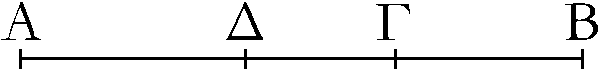
\includegraphics{Book10/fig042g.pdf}}

\gr{>'Εστω ἐκ δύο μέσων πρώτη ἡ ΑΒ διῃρημένη κατὰ τὸ Γ, <ώστε
τὰξ ΑΓ, ΓΒ μέσαξ ε>ῖναι δυνάμει μόνον συμμέτρουξ <ρητὸν
περιεθούσαξ; λέγω, <ότι ἡ ΑΒ κατ> >άλλο σημεῖον οὐ
διαιρεῖται.}

\gr{Εἰ γὰρ δυνατόν διῃρήσθω καὶ κατὰ τὸ Δ, <ώστε καὶ τὰξ ΑΔ, ΔΒ μέσαξ
ε>ῖναι δυνάμει μόνον συμμέτρουξ <ρητὸν περιεθούσαξ. ἐπεὶ
ο>ῦν, <ῶ| διαφέρει τὸ δὶξ ὑπὸ τῶν ΑΔ, ΔΒ τοῦ δὶξ
ὑπὸ τῶν ΑΓ, ΓΒ, τούτῳ διαφέρει τὰ ἀπὸ τῶν ΑΓ, ΓΒ τῶν ἀπὸ
τῶν ΑΔ, ΔΒ, <ρητῶ| δὲ διαφέρει τὸ δὶξ ὑπὸ τῶν ΑΔ, ΔΒ
τοῦ δὶξ ὑπὸ τῶν ΑΓ, ΓΒ; <ρητὰ γὰρ ἀμφότερα; <ρητῶ|
>άρα διαφέρει καὶ τὰ ἀπὸ τῶν ΑΓ, ΓΒ τῶν ἀπὸ τῶν ΑΔ, ΔΒ μέσα
>όντα; <όπερ >άτοπον.}

\gr{Οὐκ >άρα ἡ ἐκ δύο μέσων πρώτη κατ> >άλλο καὶ >άλλο
σημεῖον διαιρεῖται εἰξ τὰ ὀνόματα; καθ> <ὲν >άρα
μόνον; <όπερ >έδει δεῖχαι.}}

\ParallelRText{
\begin{center}
{\large Proposition 43}
\end{center}

A first bimedial (straight-line) can be divided (into its component terms) at
one point only.$^\dag$

% Removed epsf size command
\centerline{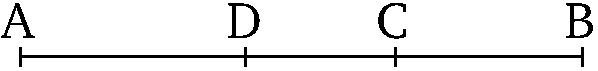
\includegraphics{Book10/fig042e.pdf}}

Let $AB$ be a first bimedial (straight-line) which has been divided at $C$, such
that $AC$ and $CB$ are medial (straight-lines), commensurable
in square only, (and) containing a rational (area) [Prop.~10.37].  I say that $AB$ cannot be (so) divided
at another point.

For, if possible, let it also be divided at $D$, such that $AD$ and
$DB$ are also medial (straight-lines), commensurable in square only, (and)
containing a rational (area). Since, therefore, by whatever (amount) twice the
(rectangle contained) by $AD$ and $DB$ differs from twice the (rectangle
contained) by $AC$ and $CB$, (the sum of) the (squares)
on $AC$ and $CB$ differs from (the sum of) the (squares) on $AD$ and
$DB$ by this (same amount) [Prop.~10.41~lem.]. And twice the (rectangle
contained) by  $AD$ and $DB$ differs from twice the (rectangle contained)
by $AC$ and $CB$ by a rational (area). For (they are) both
rational (areas). (The sum of) the (squares) on $AC$ and $CB$
thus differs from (the sum of) the (squares) on $AD$ and $DB$ by a
rational (area, despite both) being medial (areas). The very thing is
absurd [Prop.~10.26].

Thus,  a first bimedial (straight-line) cannot be divided into its (component)
terms at different points. Thus, (it can be so divided) at one
point only.
(Which is) the very thing it was required to show.}
\end{Parallel}
{\footnotesize\noindent$^\dag$ In other words, $k^{1/4} + k^{3/4} = k'^{1/4} + k'^{3/4}$
has only one solution: {i.e.}, $k'=k$.} 

%%%%%%
% Prop 10.44
%%%%%%
\pdfbookmark[1]{Proposition 10.44}{pdf10.44}
\begin{Parallel}{}{} 
\ParallelLText{
\begin{center}
{\large \ggn{44}.}
\end{center}\vspace*{-7pt}

\gr{Ἡ ἐκ δύο μέσων δευτέρα καθ> <ὲν μόνον σημεῖον διαιρεῖται.}

\gr{>'Εστω ἐκ δύο μέσων δευτέρα ἡ ΑΒ διῃρημένη κατὰ τὸ Γ, <ώστε
τὰξ ΑΓ, ΓΒ μέσαξ ε>ῖναι δυνάμει μόνον συμμέτρουξ μέσον
περιεθούσαξ; φανερὸν δή, <ότι τὸ Γ οὐκ >έστι κατὰ τῆξ διθοτομίαξ,
<ότι οὐκ εἰσὶ μ\kern -.7pt  ήκει σύμμετροι. λέγω, <ότι ἡ ΑΒ κατ> >άλλο
σημεῖον οὐ διαιρεῖται.}\\~\\~\\

% Removed epsf size command
\centerline{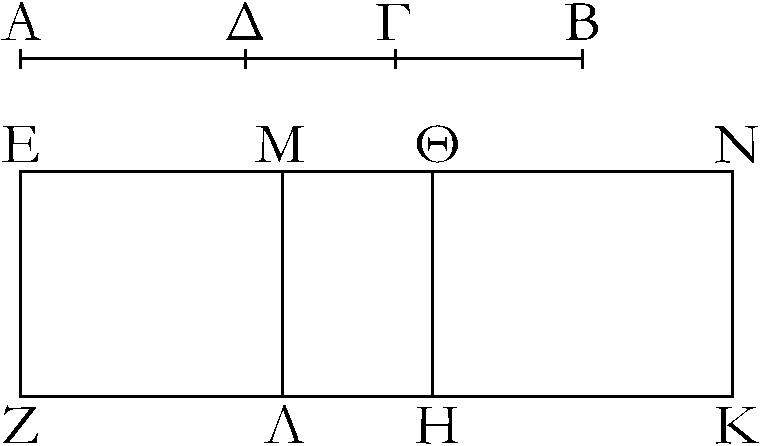
\includegraphics{Book10/fig044g.pdf}}

\gr{Εἰ γὰρ δυνατόν, διῃρήσθω καὶ κατὰ τὸ Δ, <ώστε τὴν ΑΓ τῆ|
ΔΒ μ\kern -.7pt  ὴ ε>ῖναι τὴν α\kern -.7pt  ὐτήν, ἀλλὰ μείζονα καθ> ὑπόθεσιν τὴν ΑΓ;
δῆλον δή, <ότι καὶ τὰ ἀπὸ τῶν ΑΔ, ΔΒ, ὡξ ἐπάνω ἐδείχαμεν,
ἐλάσσονα τῶν ἀπὸ τῶν ΑΓ, ΓΒ; καὶ τὰξ ΑΔ, ΔΒ μέσαξ ε>ῖναι
δυνάμει μόνον συμμέτρουξ μέσον περιεθούσαξ. καὶ ἐκκείσθω
<ρητὴ ἡ ΕΖ, καὶ τῶ| μὲν ἀπὸ τῆξ ΑΒ >ίσον παρὰ τὴν ΕΖ
παραλληλόγραμμον ὀρθογώνιον παραβεβλήσθω τὸ ΕΚ, τοῖξ
δὲ ἀπὸ τῶν ΑΓ, ΓΒ >ίσον ἀφῃρήσθω τὸ ΕΗ; λοιπὸν >άρα τὸ ΘΚ
>ίσον ἐστὶ τῶ| δὶξ ὑπὸ τῶν ΑΓ, ΓΒ. πάλιν δὴ τοῖξ ἀπὸ
τῶν ΑΔ, ΔΒ, <άπερ ἐλάσσονα ἐδείθθη τῶν ἀπὸ τῶν ΑΓ, ΓΒ, >ίσον
ἀφῃρήσθω τὸ ΕΛ; καὶ λοιπὸν >άρα τὸ ΜΚ >ίσον τῶ| δὶξ ὑπὸ τῶν
ΑΔ, ΔΒ. καὶ ἐπεὶ μέσα ἐστὶ τὰ ἀπὸ τῶν ΑΓ, ΓΒ, μέσον >άρα [καὶ]
τὸ ΕΗ. καὶ παρὰ <ρητὴν τὴν ΕΖ παράκειται; <ρητὴ >άρα ἐστὶν
ἡ ΕΘ καὶ ἀσύμμετροξ τῆ| ΕΖ μ\kern -.5pt  ήκει. διὰ τὰ α\kern -.3pt  ὐτὰ δὴ  καὶ ἡ ΘΝ
<ρητή ἐστι καὶ ἀσύμμετροξ τῆ| ΕΖ μ\kern -.7pt  ήκει. καὶ ἐπεὶ αἱ
ΑΓ, ΓΒ μέσαι εἰσὶ δυνάμει μόνον σύμμετροι, ἀσύμμετροξ >άρα
ἐστὶν ἡ ΑΓ τῆ| ΓΒ μ\kern -.7pt  ήκει. ὡξ δὲ ἡ ΑΓ πρὸξ τὴν ΓΒ, ο<ύτωξ
τὸ ἀπὸ τῆξ ΑΓ πρὸξ τὸ ὑπὸ τῶν ΑΓ, ΓΒ; ἀσύμμετρον
>άρα ἐστὶ τὸ ἀπὸ τῆξ ΑΓ τῶ| ὑπὸ τῶν ΑΓ, ΓΒ. ἀλλὰ
τῶ| μὲν ἀπὸ τῆξ ΑΓ σύμμετρά ἐστι τὰ ἀπὸ τῶν ΑΓ, ΓΒ; δυνάμει
γάρ εἰσι σύμμετροι αἱ ΑΓ, ΓΒ. τῶ| δὲ ὑπὸ τῶν ΑΓ, ΓΒ σύμμετρόν
ἐστι τὸ δὶξ ὑπὸ τῶν ΑΓ, ΓΒ. καὶ τὰ ἀπὸ τῶν ΑΓ, ΓΒ >άρα ἀσύμμετρά ἐστι τῶ| δὶξ ὑπὸ τῶν ΑΓ, ΓΒ. ἀλλὰ τοῖξ μὲν ἀπὸ
τῶν ΑΓ, ΓΒ >ίσον ἐστὶ τὸ ΕΗ, τῶ| δὲ δὶξ ὑπὸ τῶν ΑΓ, ΓΒ
>ίσον τὸ ΘΚ; ἀσύμμετρον >άρα ἐστὶ τὸ ΕΗ τῶ| ΘΚ; <ώστε καὶ ἡ
ΕΘ τῆ| ΘΝ ἀσύμμετρόξ ἐστι μ\kern -.7pt  ήκει. καί εἰσι <ρηταί; αἱ ΕΘ, ΘΝ
>άρα <ρηταί εἰσι δυνάμει μόνον σύμμετροι.
ἒαν δὲ δύο <ρηταὶ δυνάμει μόνον σύμμετροι
 συντεθῶσιν, ἡ <όλη 
>άλογόξ ἐστιν ἡ καλουμένη ἐκ δύο ὀνομάτων;
ἡ ΕΝ >άρα ἐκ δύο ὀνομάτων ἐστὶ διῃρημένη κατὰ τὸ
Θ. κατὰ τὰ α\kern -.7pt  ὐτὰ δὴ δειθθήσονται καὶ αἱ ΕΜ, ΜΝ
<ρηταὶ δυνάμει μόνον σύμμετροι; καὶ >έσται ἡ ΕΝ ἐκ δύο
ὀνομάτων κατ> >άλλο καὶ >άλλο διῃρημένη τό τε Θ καὶ τὸ Μ, καὶ
οὐκ >έστιν ἡ ΕΘ τῆ| ΜΝ ἡ α\kern -.7pt  ὐτή, <ότι
τὰ ἀπὸ τῶν ΑΓ, ΓΒ μείζονά ἐστι τῶν ἀπὸ τῶν ΑΔ, ΔΒ.
ἀλλὰ τὰ ἀπὸ τῶν ΑΔ, ΔΒ μείζονά ἐστι τοῦ δὶξ ὑπὸ
 ΑΔ, ΔΒ; πολλῶ| >άρα καὶ τὰ ἀπὸ τῶν ΑΓ, ΓΒ,
 τουτέστι τὸ ΕΗ, μεῖζόν ἐστι τοῦ δὶξ ὑπὸ τῶν ΑΔ, ΔΒ, τουτέστι
 τοῦ 
  ΜΚ; <ώστε καὶ ἡ ΕΘ τῆξ ΜΝ
μείζων ἐστίν. ἡ >άρα ΕΘ τῆ| ΜΝ οὐκ >έστιν ἡ α\kern -.7pt  ὐτή;
<όπερ >έδει δεῖχαι.}}

\ParallelRText{
\begin{center}
{\large Proposition 44}
\end{center}

A second bimedial (straight-line)  can be divided
(into its component terms)
at one point only.$^\dag$

Let $AB$ be a second bimedial (straight-line) which has  been divided at $C$, so that $AC$ and $BC$ are medial (straight-lines), commensurable in square
only, (and) containing a medial (area) [Prop.~10.38].
So, (it is) clear that $C$ is not 
(located) at the point of bisection, since ($AC$ and $BC$)
are not commensurable in length. I say that $AB$ cannot be (so) divided at another point.

% Removed epsf size command
\centerline{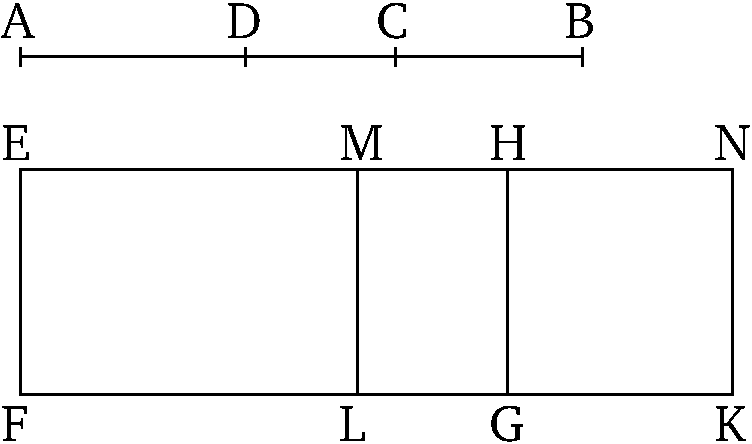
\includegraphics{Book10/fig044e.pdf}}

For, if possible, let it also have  been (so) divided at $D$, so that $AC$ is not the
same as $DB$, but $AC$ (is), by hypothesis, greater. So, (it is)  clear that
(the sum of) the (squares) on $AD$ and $DB$ is also less than (the sum of)
the (squares) on $AC$ and $CB$, as we showed above [Prop.~10.41~lem.].  And $AD$ and $DB$ are medial (straight-lines), commensurable in square only, (and)
containing a medial (area). And let the rational (straight-line) $EF$
be laid down. And let the rectangular parallelogram $EK$, equal to the (square) on $AB$, be applied to $EF$. And let $EG$, equal to
(the sum of) the (squares) on $AC$ and $CB$, be cut  off (from $EK$).
Thus, the remainder, $HK$, is equal to twice the (rectangle contained)
by $AC$ and $CB$ [Prop.~2.4]. So, again,
let $EL$, equal to  (the sum of) the (squares) on  $AD$ and $DB$---which was shown (to be) less than (the sum of) the (squares) on $AC$ and
$CB$---be cut off (from $EK$). And, thus, the remainder, $MK$,
(is) equal to twice the (rectangle contained) by $AD$ and $DB$. 
And since (the sum of) the (squares) on $AC$ and $CB$ is medial, $EG$ (is) thus [also]
medial. And it is applied to the rational (straight-line) $EF$. Thus, $EH$
is rational, and incommensurable in length with $EF$ [Prop.~10.22]. So, for the same (reasons), $HN$
is also rational, and incommensurable in length with $EF$. And since 
$AC$ and $CB$  are medial (straight-lines which are) commensurable
in square only, $AC$ is thus incommensurable in length with $CB$.
And as $AC$ (is) to $CB$, so the (square) on $AC$ (is) to the
(rectangle contained) by $AC$ and $CB$ [Prop.~10.21~lem.]. Thus, the (square) on $AC$ is
incommensurable with the (rectangle contained) by $AC$ and $CB$
[Prop.~10.11]. But, (the sum of) the (squares)
on $AC$ and $CB$ is commensurable with the (square) on $AC$.
For, $AC$ and $CB$ are commensurable in square [Prop.~10.15]. And
twice the (rectangle contained) by $AC$ and $CB$ is commensurable with the (rectangle contained) by $AC$ and $CB$ [Prop.~10.6]. And thus
(the sum of) the squares on $AC$ and $CB$ is incommensurable with twice
the (rectangle contained) by $AC$ and $CB$ [Prop.~10.13]. But, $EG$ is equal to (the sum
of) the (squares) on $AC$ and $CB$, and $HK$ equal to twice the (rectangle
contained) by $AC$ and $CB$. Thus, $EG$ is incommensurable
with $HK$. Hence, $EH$ is also incommensurable in length with  $HN$
[Props.~6.1, 10.11].
And (they are)  rational (straight-lines). Thus, $EH$ and $HN$ are rational
(straight-lines which are) commensurable in square only. And if two
rational (straight-lines which are) commensurable in square only are
added together then the whole (straight-line) is that irrational called
binomial [Prop.~10.36]. Thus, $EN$
is a binomial (straight-line) which has been divided (into its component terms) at $H$. So, according to
the same (reasoning), $EM$ and $MN$ can be shown (to be) rational
(straight-lines which are) commensurable in square only. And $EN$
will (thus) be a binomial (straight-line) which has been divided (into its component terms) at the different (points)
$H$ and $M$ (which is absurd [Prop.~10.42]).
And $EH$ is not the same as $MN$, since (the sum of) the
(squares) on $AC$ and $CB$ is greater than (the sum of) the (squares) on
$AD$ and $DB$. But, (the sum of) the (squares) on $AD$ and $DB$
is greater than twice the (rectangle contained) by $AD$ and $DB$ [Prop.~10.59~lem.]. Thus,  (the sum of) the (squares) on $AC$ and $CB$---that is to say, $EG$---is also much greater than twice the (rectangle contained) by 
$AD$ and $DB$---that is to say, $MK$. Hence, $EH$ is also greater
than $MN$ [Prop.~6.1]. Thus, $EH$ is not the same as $MN$. (Which is) the very thing
it was required to show.}
\end{Parallel}
{\footnotesize\noindent$^\dag$ In other words, $k^{1/4}+k'^{1/2}/k^{1/4}
= k''^{1/4}+k'''^{1/2}/k''^{1/4}$
has only one solution: {i.e.}, $k''=k$ and $k'''=k'$.}

%%%%%%
% Prop 10.45
%%%%%%
\pdfbookmark[1]{Proposition 10.45}{pdf10.45}
\begin{Parallel}{}{} 
\ParallelLText{\
\begin{center}
{\large\ggn{45}.}
\end{center}\vspace*{-7pt}

\gr{Ἡ μείζων κατὰ τὸ α\kern -.7pt  ὐτὸ μόνον σημεῖον διαιρεῖται.}\\

% Removed epsf size command
\centerline{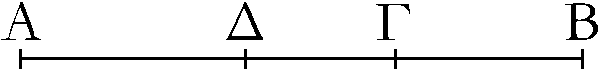
\includegraphics{Book10/fig042g.pdf}}

\gr{>'Εστω μείζων ἡ ΑΒ διῃρημένη κατὰ τὸ Γ, <ώστε τὰξ ΑΓ, ΓΒ
δυνάμει ἀσυμμέτρουξ ε>ῖναι ποιούσαξ τὸ μὲν συγκείμενον
ἐκ τῶν ἀπὸ τῶν ΑΓ, ΓΒ τετραγώνων <ρητόν, τὸ δ> ὑπὸ
τῶν ΑΓ, ΓΒ μέσον; λέγω, <ότι ἡ ΑΒ κατ> >άλλο σημεῖον οὐ
διαιρεῖται.}

\gr{Εἰ γὰρ δυνατόν, διῃρήσθω καὶ κατὰ τὸ Δ, <ώστε καὶ τὰξ ΑΔ, ΔΒ δυνάμει
ἀσυμμέτρουξ ε>ῖναι ποιούσαξ τὸ μὲν συγκείμενον ἐκ τῶν
ἀπὸ τῶν ΑΔ, ΔΒ <ρητόν, τὸ δ> ὑπ> α\kern -.7pt  ὐτῶν μέσον. καὶ ἐπεί,
<ῶ| διαφέρει τὰ ἀπὸ τῶν ΑΓ, ΓΒ τῶν ἀπὸ τῶν ΑΔ, ΔΒ,
τούτῳ διαφέρει καὶ τὸ δὶξ ὑπὸ τῶν ΑΔ, ΔΒ τοῦ δὶξ ὑπὸ
τῶν ΑΓ, ΓΒ, ἀλλὰ τὰ ἀπὸ τῶν ΑΓ, ΓΒ τῶν ἀπὸ τῶν
ΑΔ, ΔΒ ὑπερέθει <ρητῶ|; <ρητὰ γὰρ ἀμφότερα; καὶ τὸ δὶξ ὑπὸ
τῶν ΑΔ, ΔΒ >άρα τοῦ δὶξ ὑπὸ τῶν
ΑΓ, ΓΒ ὑπερέθει <ρητῶ| μέσα >όντα; <όπερ ἐστὶν
ἀδύνατον. οὐκ >άρα ἡ μείζων κατ> >άλλο καὶ >άλλο
σημεῖον διαιρεῖται; κατὰ τὸ α\kern -.7pt  ὐτὸ >άρα μόνον διαιρεῖται;
<όπερ >έδει δεῖχαι.}}

\ParallelRText{
\begin{center}
{\large Proposition 45}
\end{center}

A major (straight-line) can only  be divided (into
its component terms) at the same
point.$^\dag$

% Removed epsf size command
\centerline{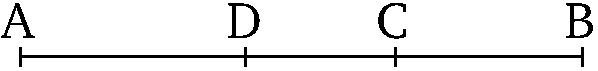
\includegraphics{Book10/fig042e.pdf}}

Let $AB$ be a major (straight-line) which has been divided at $C$, so
that $AC$ and $CB$ are incommensurable in square, making the sum
of the squares on $AC$ and $CB$ rational, and the (rectangle contained)
by $AC$ and $CD$ medial [Prop.~10.39].
I say that $AB$ cannot be (so) divided at another point.

For, if possible, let it also be divided at $D$, such that $AD$ and
$DB$ are also incommensurable in square, making the
sum of the (squares) on $AD$ and $DB$ rational, and the (rectangle contained) by them medial. And since, by whatever (amount the sum of)
the (squares) on $AC$ and $CB$ differs from (the sum of) the (squares)
on $AD$ and $DB$, 
twice the (rectangle contained) by $AD$ and $DB$ also differs from
twice the (rectangle contained) by $AC$ and $CB$ by this (same amount). But, (the sum of) the
(squares) on $AC$ and $CB$ exceeds (the sum of) the (squares) on
$AD$ and $DB$ by a rational (area). For (they are) both rational (areas). Thus, twice the
(rectangle contained) by $AD$ and $DB$ also exceeds twice the
(rectangle contained) by $AC$ and $CB$ by a rational (area), (despite both) being medial (areas).
The very thing is impossible [Prop.~10.26].
Thus, a major (straight-line) cannot be divided (into its component terms) at different points. Thus,
it can only be (so) divided at the same (point). (Which is) the very thing it was required to show.}
\end{Parallel}
{\footnotesize\noindent$^\dag$ In other words, $\sqrt{[1+k/(1+k^2)^{1/2}]/2} + \sqrt{[1-k/(1+k^2)^{1/2}]/2} =\sqrt{[1+k'/(1+k'^2)^{1/2}]/2} + \sqrt{[1-k'/(1+k'^2)^{1/2}]/2}$ has only one solution: {i.e.}, $k'=k$.}

%%%%%%
% Prop 10.46
%%%%%%
\pdfbookmark[1]{Proposition 10.46}{pdf10.46}
\begin{Parallel}{}{} 
\ParallelLText{
\begin{center}
{\large \ggn{46}.}
\end{center}\vspace*{-7pt}

\gr{Ἡ <ρητὸν καὶ μέσον δυναμένη καθ> <ὲν μόνον σημεῖον διαιρεῖται.}

% Removed epsf size command
\centerline{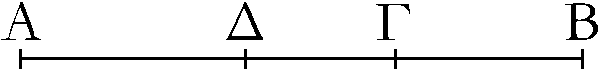
\includegraphics{Book10/fig042g.pdf}}

\gr{>'Εστω <ρητὸν καὶ μέσον δυναμένη ἡ ΑΒ διῃρημένη κατὰ τὸ Γ, <ώστε
τὰξ ΑΓ, ΓΒ δυνάμει ἀσυμμέτρουξ ε>ῖναι ποιούσαξ τὸ μὲν συγκείμενον ἐκ τῶν ἀπὸ τῶν ΑΓ, ΓΒ μέσον, τὸ δὲ δὶξ ὑπὸ
τῶν ΑΓ, ΓΒ <ρητόν; λέγω, <ότι ἡ ΑΒ κατ> >άλλο σημεῖον
οὐ διαιρεῖται.}

\gr{Εἰ γὰρ δυνατόν, διῃρήσθω καὶ κατὰ τὸ Δ, <ώστε καὶ τὰξ ΑΔ, ΔΒ
δυνάμει ἀσυμμέτρουξ ε>ῖναι ποιούσαξ τὸ μὲν συγκείμενον
ἐκ τῶν ἀπὸ τῶν ΑΔ, ΔΒ μέσον, τὸ δὲ δὶξ ὑπὸ
τῶν ΑΔ, ΔΒ <ρητόν. ἐπεὶ ο>ῦν, <ῶ| διαφέρει τὸ δὶξ ὑπὸ
τῶν ΑΓ, ΓΒ τοῦ δὶξ ὑπὸ τῶν ΑΔ, ΔΒ, τούτῳ διαφέρει καὶ
τὰ ἀπὸ τῶν ΑΔ, ΔΒ τῶν ἀπὸ τῶν ΑΓ, ΓΒ, τὸ δὲ δὶξ ὑπὸ
τῶν ΑΓ, ΓΒ 
 τοῦ δὶξ ὑπὸ τῶν ΑΔ, ΔΒ ὑπερέθει
<ρητῶ|, καὶ τὰ ἀπὸ τῶν ΑΔ, ΔΒ >άρα τῶν ἀπὸ τῶν ΑΓ, ΓΒ
ὑπερέθει <ρητῶ| μέσα >όντα; <όπερ ἐστὶν ἀδύνατον. οὐκ
>άρα ἡ <ρητὸν καὶ μέσον δυναμένη κατ> >άλλο
καὶ >άλλο σημεῖον διαιρεῖται. κατὰ <ὲν >άρα σημεῖον
διαιρεῖται; <όπερ >έδει δεῖχαι.}}

\ParallelRText{
\begin{center}
{\large Proposition 46}
\end{center}
The square-root of a rational plus a  medial
(area) can be divided (into its component terms) at  one point only.$^\dag$

% Removed epsf size command
\centerline{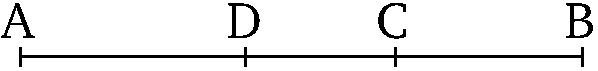
\includegraphics{Book10/fig042e.pdf}}

Let $AB$ be the square-root of a rational plus a medial (area) which has
been divided at $C$, so that $AC$ and $CB$ are incommensurable
in square, making the sum of the (squares) on $AC$ and $CB$ medial,
and twice the (rectangle contained) by $AC$ and $CB$ rational
[Prop.~10.40]. I say that $AB$ cannot be (so)
divided at another point.

For, if possible, let it also be divided at $D$, so that
$AD$ and $DB$ are also incommensurable in square, making the sum of 
the (squares) on $AD$ and $DB$ medial, and twice the (rectangle
contained) by $AD$ and $DB$ rational. Therefore, since by whatever
(amount) twice the (rectangle contained) by $AC$ and $CB$
differs from twice the (rectangle contained) by $AD$ and $DB$, (the sum of) the (squares) on  $AD$ and $DB$ also differs from (the sum of) the
(squares) on
$AC$ and $CB$ by this
(same amount). And twice the (rectangle contained) by $AC$ and $CB$
exceeds twice the (rectangle contained) by $AD$ and $DB$ by a
rational (area). (The sum of) the (squares)
on $AD$ and $DB$ thus also exceeds (the sum of) the (squares) on $AC$ and $CB$ by a rational (area),
(despite both) being medial (areas). The very thing is impossible [Prop.~10.26]. Thus, the square-root of a rational
plus a medial (area) cannot be divided (into its component terms) at different points. Thus, it
can  be (so) divided at one point (only). (Which is) the very thing it was required to
show.}
\end{Parallel}
{\footnotesize\noindent$^\dag$ In other words, $\sqrt{[(1+k^2)^{1/2}+k]/[2\,(1+k^2)]} +\sqrt{[(1+k^2)^{1/2}-k]/[2\,(1+k^2)]}=\sqrt{[(1+k'^2)^{1/2}+k']/[2\,(1+k'^2)]}$\\$ +\sqrt{[(1+k'^2)^{1/2}-k']/[2\,(1+k'^2)]}$
has only one solution: {i.e.}, $k'=k$.}

%%%%%%
% Prop 10.47
%%%%%%
\pdfbookmark[1]{Proposition 10.47}{pdf10.47}
\begin{Parallel}{}{} 
\ParallelLText{
\begin{center}
{\large \ggn{47}.}
\end{center}\vspace*{-7pt}

\gr{Ἡ δύο μέσα δυναμένη καθ> <ὲν μόνον σημεῖον διαιρεῖται.}\\

% Removed epsf size command
\centerline{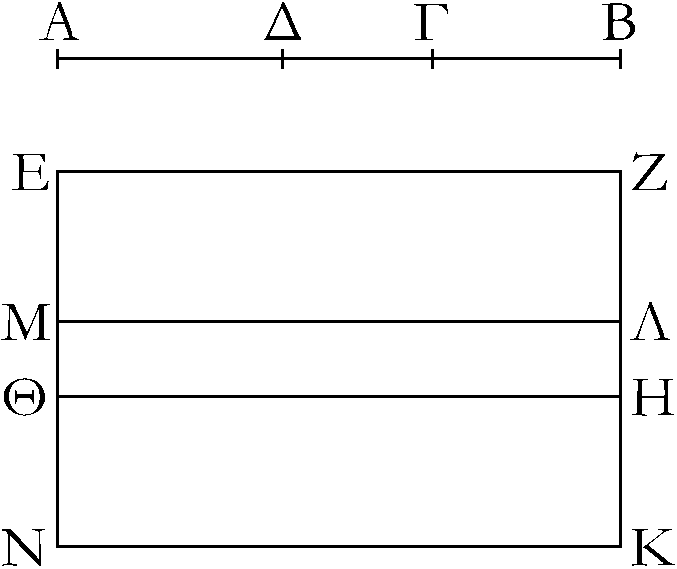
\includegraphics{Book10/fig047g.pdf}}

\gr{>'Εστω [δύο μέσα δυναμένη] ἡ ΑΒ διῃρημένη κατὰ τὸ Γ, <ώστε τὰξ
ΑΓ, ΓΒ δυνάμει ἀσυμμέτρουξ ε>ῖναι ποιούσαξ τό τε συγκείμενον
ἐκ τῶν ἀπὸ τῶν ΑΓ, ΓΒ μέσον καὶ τὸ ὑπὸ τῶν ΑΓ, ΓΒ μέσον
καὶ >έτι ἀσύμμετρον τῶ| συγκειμένῳ ἐκ τῶν ἀπ> α\kern -.7pt  ὐτῶν.
λέγω, <ότι ἡ ΑΒ κατ> >άλλο σημεῖον οὐ διαιρεῖται ποιοῦσα
τὰ προκείμενα.}

\gr{Εἰ γὰρ δυνατόν, διῃρήσθω κατὰ τὸ Δ, <ώστε πάλιν δηλονότι
τὴν ΑΓ τῆ| ΔΒ μ\kern -.7pt  ὴ ε>ῖναι τὴν α\kern -.7pt  ὐτήν, ἀλλὰ μείζονα καθ> ὑπόθεσιν
τὴν ΑΓ, καὶ ἐκκείσθω <ρητὴ ἡ ΕΖ, καὶ παραβεβλήσθω παρὰ τὴν ΕΖ
τοῖξ μὲν ἀπὸ τῶν ΑΓ, ΓΒ >ίσον τὸ ΕΗ, τῶ| δὲ δὶξ ὑπὸ τῶν
ΑΓ, ΓΒ >ίσον τὸ ΘΚ; <όλον >άρα τὸ ΕΚ >ίσον ἐστὶ τῶ| ἀπὸ
τῆξ ΑΒ  τετραγώνῳ. πάλιν δὴ παραβεβλήσθω παρὰ τὴν ΕΖ τοῖξ ἀπὸ
τῶν ΑΔ, ΔΒ >ίσον τὸ ΕΛ; λοιπὸν >άρα τὸ δὶξ ὑπὸ τῶν ΑΔ, ΔΒ
λοιπῶ| τῶ| ΜΚ >ίσον ἐστίν. καὶ ἐπεὶ μέσον ὑπόκειται τὸ συγκείμενον ἐκ τῶν ἀπὸ τῶν ΑΓ, ΓΒ, μέσον >άρα ἐστὶ καὶ
τὸ ΕΗ. καὶ παρὰ <ρητὴν τὴν ΕΖ παράκειται; <ρητὴ >άρα ἐστὶν
ἡ ΘΕ καὶ ἀσύμμετροξ τῆ| ΕΖ μ\kern -.5pt  ήκει. διὰ τὰ α\kern -.3pt  ὐτὰ δὴ καὶ ἡ ΘΝ
<ρητή ἐστι καὶ ἀσύμμετροξ τῆ| ΕΖ μ\kern -.7pt  ήκει. καὶ ἐπεὶ ἀσύμμετρόν
ἐστι τὸ συγκείμενον ἐκ τῶν ἀπὸ τῶν ΑΓ, ΓΒ τῶ| δὶξ ὑπὸ τῶν ΑΓ, ΓΒ, καὶ τὸ ΕΗ >άρα τῶ| ΗΝ ἀσύμμετρόν ἐστιν; <ώστε
καὶ ἡ ΕΘ τῆ| ΘΝ ἀσύμμετρόξ ἐστιν. καί εἰσι <ρηταί; αἱ ΕΘ,
ΘΝ >άρα <ρηταί εἰσι δυνάμει μόνον σύμμετροι; ἡ ΕΝ >άρα ἐκ
δύο ὀνομάτων ἐστὶ διῃρημένη κατὰ τὸ Θ. ὁμοίωξ
δὴ δείχομεν, <ότι καὶ κατὰ τὸ Μ διή|ρηται. καὶ οὐκ >έστιν ἡ ΕΘ
τῆ| ΜΝ ἡ α\kern -.7pt  ὐτή; ἡ >άρα ἐκ δύο ὀνομάτων κατ> >άλλο καὶ >άλλο
σημεῖον διή|ρηται; <όπερ ἐστίν >άτοπον. οὐκ >άρα ἡ δύο
μέσα δυναμένη κατ> ἀλλο καὶ >άλλο σημεῖον διαιρεῖται;
καθ> <ὲν >άρα μόνον [σημεῖον] διαιρεῖται.}}

\ParallelRText{
\begin{center}
{\large Proposition 47}
\end{center}

The square-root of (the sum of) two medial (areas) can be
divided (into its component terms) at one point only.$^\dag$

% Removed epsf size command
\centerline{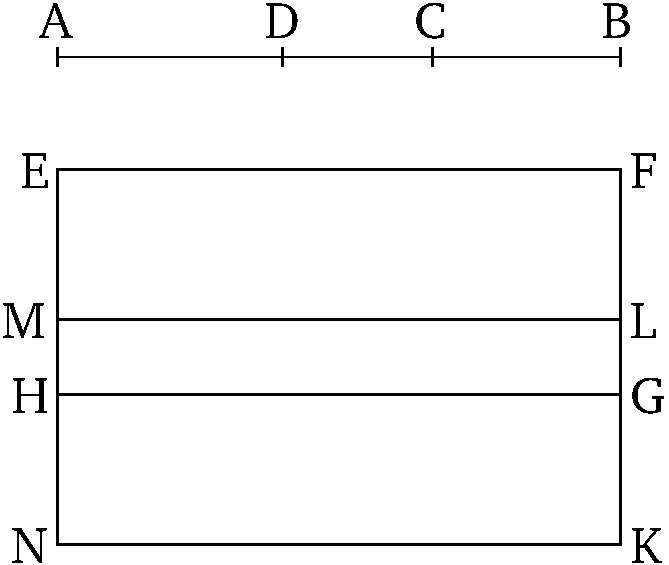
\includegraphics{Book10/fig047e.pdf}}

Let $AB$ be [the square-root of (the sum of) two medial (areas)] which has been divided
at $C$, such that $AC$ and $CB$ are incommensurable in square, making the
sum of the (squares) on $AC$ and $CB$ medial, and the (rectangle contained) by $AC$ and $CB$ medial, and, moreover, incommensurable
with the sum of the (squares) on ($AC$ and $CB$) [Prop.~10.41]. I say that $AB$ cannot be divided
at another point fulfilling the prescribed (conditions).

For, if possible, let it be divided at $D$, such that $AC$ is again
manifestly not the same as $DB$, but $AC$ (is), by hypothesis, greater.
And let the rational (straight-line) $EF$ be laid down. And let $EG$,
equal to (the sum of) the (squares) on $AC$ and $CB$, and $HK$, equal to twice the (rectangle contained) by $AC$ and $CB$,
be applied to $EF$. Thus, the whole of $EK$ is equal to the
square on $AB$ [Prop.~2.4]. So, again, let $EL$, equal to (the sum of) the (squares)
on $AD$ and $DB$, be applied to $EF$. Thus, the remainder---twice
the (rectangle contained) by $AD$ and $DB$---is equal to the remainder, $MK$. And since the sum of the (squares) on $AC$ and $CB$
was assumed (to be) medial, $EG$ is also medial. And it is applied
to the rational (straight-line) $EF$. $HE$ is thus rational, and incommensurable in length with $EF$ [Prop.~10.22].  So, for the same (reasons), 
$HN$ is also rational, and incommensurable in length with $EF$.
And since the sum of the (squares) on $AC$ and $CB$ is incommensurable
with twice the (rectangle contained) by $AC$ and $CB$, $EG$ is thus also
incommensurable with $GN$. Hence, $EH$ is also incommensurable with
$HN$ [Props.~6.1, 10.11].
And they are (both) rational (straight-lines). Thus, $EH$ and $HN$ are rational
(straight-lines which are) commensurable in  square only. Thus, $EN$
is a binomial (straight-line) which has been divided (into its component
terms) at $H$ [Prop.~10.36]. So, similarly, we can show that
it has also been (so) divided at $M$. And $EH$ is not the same  as $MN$. Thus,
a binomial (straight-line) has been divided (into its component
terms) at different points. The
very thing is absurd [Prop.~10.42]. Thus,
the square-root of (the sum of) two medial (areas) cannot be divided (into its component terms) at different
points. Thus, it can be (so) divided at one [point] only.}
\end{Parallel}
{\footnotesize\noindent$^\dag$ In other words, $k'^{1/4}\sqrt{[1+k/(1+k^2)^{1/2}]/2}
+k'^{1/4}\sqrt{[1-k/(1+k^2)^{1/2}]/2}=k'''^{1/4}\sqrt{[1+k''/(1+k''^2)^{1/2}]/2}$\\$
+k'''^{1/4}\sqrt{[1-k''/(1+k''^2)^{1/2}]/2}$ has only one solution: {i.e.}, $k''=k$ and $k'''=k'$.}

%%%%%%%%
% Definitions 2
%%%%%%%%
\pdfbookmark[1]{Definitions II}{def10.2}
\begin{Parallel}{}{} 
\ParallelLText{
\begin{center}
\large{\gr{<'Οροι δεύτεροι}.}
\end{center}\vspace*{-7pt}

\ggn{5}.~\gr{Ὑποκειμένηξ <ρητῆξ καὶ τῆξ ἐκ δύο ὀνομάτων
διῃρημένηξ εἰξ τὰ ὀνόματα, <ῆξ τὸ μεῖζον >όνομα
τοῦ ἐλάσσονοξ μεῖζον δύναται τῶ| ἀπὸ συμμέτρου ἑαυτῆ|
μ\kern -.7pt  ήκει, ἒαν μὲν τὸ μεῖζον >όνομα σύμμετρον >ῆ| μ\kern -.7pt  ήκει
τῆ| ἐκκειμένῃ <ρητῆ|, καλείσθω [ἡ <όλη] ἐκ δύο ὀνομάτων
πρώτη.}

\ggn{6}.~\gr{Ἐὰν δὲ τὸ ἐλάσσον >όνομα σύμμετρον >ῆ| μ\kern -.7pt  ήκει τῆ| ἐκκειμένῃ <ρητῆ|, καλείσθω ἐκ δύο ὀνομάτων δευτέρα.}

\ggn{7}.~\gr{Ἐὰν δὲ μ\kern -.7pt  ηδέτερον τῶν ὀνομάτων σύμμετρον >ῆ|
μ\kern -.7pt  ήκει τῆ| ἐκκειμένῃ <ρητῆ|, καλείσθω ἐκ δύο ὀνομάτων
τρίτη.}

\ggn{8}.~\gr{Πάλιν δὴ ἒαν τὸ μεῖζον >όνομα [τοῦ ἐλάσσονοξ]
μεῖζον δύνηται τῶ| ἀπὸ ἀσυμμέτρου ἑαυτῆ| μ\kern -.7pt  ήκει,
ἒαν μὲν τὸ μεῖζον >όνομα σύμμετρον >ῆ| μ\kern -.7pt  ήκει τῆ|
ἐκκειμένῃ <ρητῆ|, καλείσθω ἐκ δύο ὀνομάτων τετάρτη.}

\ggn{9}.~\gr{Ἐὰν δὲ τὸ >έλασσον, πέμπτη.}

\ggn{10}.~\gr{Ἐὰν δὲ μ\kern -.7pt  ηδέτερον, <έκτη.}}

\ParallelRText{
\begin{center}
{\large Definitions II}
\end{center}

5.~Given a rational (straight-line), and  a binomial (straight-line) which has been divided into its (component) terms, of which the square on the greater term
is larger than (the square on) the lesser  by the (square) on (some straight-line) commensurable in length with (the greater) then,
if the greater term is commensurable in length with the  rational (straight-line previously) laid out,
 let [the whole] (straight-line) be called a first binomial (straight-line).
 
6.~And if the lesser term is commensurable in length with the  rational (straight-line previously) laid
out then let (the whole straight-line) be called a
second binomial (straight-line).

7.~And if neither of the terms is commensurable in length with the 
rational (straight-line previously) laid out then let (the whole straight-line) be called a third
binomial (straight-line).

8.~So, again, if the square on the greater term is larger than (the
square on) [the lesser] by the (square) on (some straight-line)
incommensurable in length with (the greater) then, if the
greater term is commensurable in length with the  rational
(straight-line previously) laid out, let (the whole straight-line) be called a fourth
binomial (straight-line).

9.~And if the lesser (term is commensurable), a fifth (binomial straight-line).

10.~And if neither (term is commensurable), a sixth (binomial straight-line).}
\end{Parallel}

%%%%
%10.48
%%%%
\pdfbookmark[1]{Proposition 10.48}{pdf10.48}
\begin{Parallel}{}{}
\ParallelLText{
\begin{center}
{\large\ggn{48}.}
\end{center}\vspace*{-7pt}

\gr{Εὑρεῖν τὴν ἐκ δύο ὀνομάτων πρώτην.}

\gr{Ἐκκείσθωσαν δύο ἀριθμοὶ οἱ ΑΓ, ΓΒ, <ώστε τὸν συγκείμενον
ἐχ α\kern -.7pt  ὐτῶν τὸν ΑΒ πρὸξ μὲν τὸν ΒΓ λόγον >έθειν,
<ὸν τετράγωνοξ ἀριθμὸξ πρὸξ τετράγωνον ἀριθμόν, πρὸξ δὲ τὸν
ΓΑ λόγον μ\kern -.7pt  ὴ >έθειν, <ὸν τετράγωνοξ ἀριθμὸξ πρὸξ τετράγωνον
ἀριθμόν, καὶ ἐκκείσθω τιξ <ρητὴ ἡ Δ, καὶ τῆ| Δ σύμμετροξ
>έστω μ\kern -.5pt  ήκει ἡ ΕΖ. <ρητὴ >άρα ἐστὶ καὶ ἡ ΕΖ. καὶ γεγονέτω
ὡξ ὁ ΒΑ ἀριθμὸξ πρὸξ τὸν ΑΓ, ο<ύτωξ τὸ ἀπὸ τῆξ ΕΖ
πρὸξ τὸ ἀπὸ τῆξ ΖΗ. ὁ δὲ ΑΒ πρὸξ τὸν ΑΓ λόγον >έθει,
<ὸν ἀριθμὸξ πρὸξ ἀριθμόν; καὶ τὸ ἀπὸ τῆξ ΕΖ >άρα πρὸξ τὸ
ἀπὸ τῆξ ΖΗ λόγον >έθει, <ὸν ἀριθμὸξ πρὸξ ἀριθμόν; <ώστε
σύμμετρόν ἐστι τὸ ἀπὸ τῆξ ΕΖ τῶ| ἀπὸ τῆξ ΖΗ. καὶ ἐστι <ρητὴ
ἡ ΕΖ; <ρητὴ >άρα καὶ ἡ ΖΗ.
καὶ ἐπεὶ
ὁ ΒΑ πρὸξ τὸν ΑΓ λόγον οὐκ >έθει, <ὸν τετράγωνοξ ἀριθμὸξ
πρὸξ τετράγωνον ἀριθμόν, οὐδὲ τὸ ἀπὸ τῆξ ΕΖ >άρα πρὸξ τὸ
ἀπὸ τῆξ ΖΗ λόγον >έθει, <ὸν τετράγωνοξ ἀριθμὸξ πρὸξ τετράγωνον
ἀριθμόν; ἀσύμμετροξ >άρα ἐστὶν ἡ ΕΖ τῆ| ΖΗ μ\kern -.3pt  ήκει. αἱ ΕΖ,
ΖΗ >άρα <ρηταί εἰσι δυνάμει μόνον σύμμετροι; ἐκ δύο >άρα
ὀνομάτων ἐστὶν ἡ ΕΗ.
λέγω, <ότι καὶ πρώτη.}\\~\\~\\~\\~\\

% Removed epsf size command
\centerline{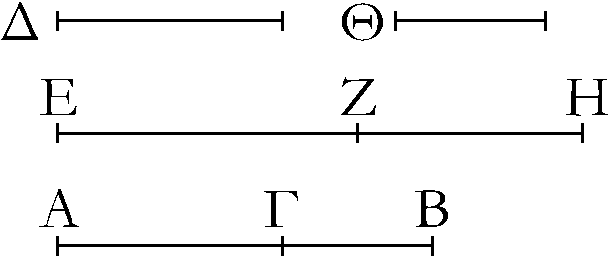
\includegraphics{Book10/fig048g.pdf}}

\gr{Ἐπεὶ γάρ ἐστιν ὡξ ὁ ΒΑ ἀριθμὸξ πρὸξ τὸν ΑΓ, ο<ύτωξ
τὸ ἀπὸ τῆξ ΕΖ πρὸξ τὸ ἀπὸ τῆξ ΖΗ, μείζων δὲ ὁ ΒΑ τοῦ
ΑΓ, μεῖζον >άρα καὶ τὸ ἀπὸ τῆξ ΕΖ τοῦ ἀπὸ τῆξ ΖΗ. >έστω
ο>ῦν τῶ| ἀπὸ τῆξ ΕΖ >ίσα τὰ ἀπὸ τῶν ΖΗ, Θ. καὶ
ἐπεί ἐστιν ὡξ ὁ ΒΑ πρὸξ τὸν ΑΓ, ο<ύτωξ τὸ ἀπὸ τῆξ
ΕΖ πρὸξ τὸ ἀπὸ τῆξ ΖΗ, ἀναστρέψαντι >άρα ἐστὶν ὡξ ὁ ΑΒ
πρὸξ τὸν ΒΓ, ο<ύτωξ τὸ ἀπὸ τῆξ ΕΖ πρὸξ τὸ ἀπὸ τῆξ Θ. ὁ δὲ
ΑΒ πρὸξ τὸν ΒΓ λόγον >έθει, <ὸν τετράγωνοξ ἀριθμὸξ πρὸξ τετράγωνον ἀριθμόν. καὶ τὸ ἀπὸ τῆξ ΕΖ >άρα πρὸξ τὸ ἀπὸ τῆξ Θ
λόγον >έθει, <ὸν τετράγωνοξ ἀριθμὸξ πρὸξ τετράγωνον ἀριθμόν.
σύμμετροξ >άρα ἐστὶν ἡ ΕΖ τῆ| Θ μ\kern -.7pt  ήκει; ἡ ΕΖ
>άρα τῆξ ΖΗ μεῖζον δύναται τῶ| ἀπὸ συμμέτρου ἑαυτῆ|. καί
εἰσι <ρηταὶ αἱ ΕΖ, ΖΗ, καὶ σύμμετροξ ἡ ΕΖ τῆ| Δ μ\kern -.7pt  ήκει.}

\gr{Ἠ ΕΗ >άρα ἐκ δύο ὀνομάτων ἐστὶ πρώτη; <όπερ
>έδει δεῖχαι.}}

\ParallelRText{
\begin{center}
{\large Proposition 48}
\end{center}

To find a first binomial (straight-line).

Let  two numbers $AC$ and $CB$ be laid down such that their sum
$AB$ has to $BC$ the ratio  which (some) square number (has) to (some)
square number, and does not have to $CA$ the ratio which (some)
square number (has) to (some) square number [Prop.~10.28~lem.~I]. And let some rational (straight-line) $D$ be laid down. And let $EF$ be commensurable in length with $D$. $EF$ is thus also rational [Def.~10.3]. 
And let it be contrived that as the number $BA$ (is) to $AC$, so the
(square) on $EF$ (is) to the (square) on $FG$ [Prop.~10.6~corr.]. And $AB$ has to $AC$ the ratio
which (some) number (has) to (some) number. Thus, the (square) on $EF$
also has to the (square) on $FG$ the ratio which (some) number
(has) to (some) number. Hence, the (square) on $EF$ is commensurable
with the (square) on $FG$ [Prop.~10.6].  And
$EF$ is rational. Thus, $FG$ (is) also rational. And since $BA$ does not
have to $AC$ the ratio which (some) square number (has) to (some)
square number, thus the (square) on $EF$ does not have to the (square)
on $FG$ the ratio which (some) square number (has) to (some) square number either. Thus, $EF$ is incommensurable in length with $FG$ [Prop~10.9]. $EF$ and $FG$ are thus rational
(straight-lines which are) commensurable in square only. Thus, $EG$
is a binomial (straight-line) [Prop.~10.36].
I say that (it is) also a first (binomial straight-line).

% Removed epsf size command
\centerline{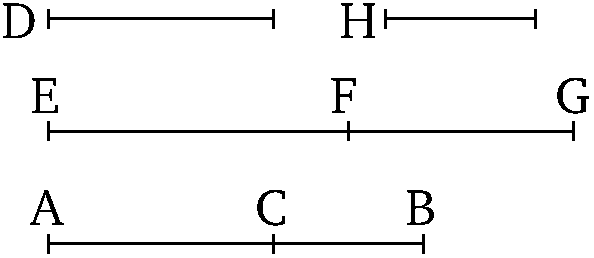
\includegraphics{Book10/fig048e.pdf}}

For since as the number $BA$ is to $AC$, so the (square) on $EF$ (is)
to the (square) on $FG$, and $BA$ (is) greater than $AC$, the
(square) on $EF$ (is) thus also greater than the (square) on $FG$ [Prop.~5.14]. Therefore, let (the sum of) the (squares)
on $FG$ and $H$ be equal to the (square) on $EF$. And since as $BA$
is to $AC$, so the (square) on $EF$ (is) to the (square) on $FG$, thus,
via conversion, as $AB$ is to $BC$, so the (square) on $EF$ (is) to
the (square) on $H$ [Prop.~5.19~corr.]. 
And $AB$ has to $BC$ the ratio which (some) square number (has) to
(some) square number. Thus, the (square) on $EF$ also has to
the (square) on $H$ the ratio which (some) square number (has) to
(some) square number. Thus,
$EF$ is commensurable in length with $H$  [Prop.~10.9]. Thus, the square on $EF$
is greater than (the square on) $FG$ by the (square) on (some straight-line)
commensurable (in length) with ($EF$). And $EF$ and $FG$ are rational (straight-lines). And $EF$ (is) commensurable in length with $D$.

Thus, $EG$ is a first binomial (straight-line) [Def.~10.5].$^\dag$
(Which is) the very thing it was required to show.}
\end{Parallel}
{\footnotesize\noindent $^\dag$If the rational straight-line has unit length then the length of a first binomial straight-line
is  $k+k\sqrt{1-k'^{\,2}}$. This, and the first apotome,
whose length is $k-k\,\sqrt{1-k'^{\,2}}$ [Prop.~10.85],
are the roots of $x^2- 2\,k\,x+k^2\,k'^{\,2}=0$.}  

%%%%
%10.49
%%%%
\pdfbookmark[1]{Proposition 10.49}{pdf10.49}
\begin{Parallel}{}{}
\ParallelLText{
\begin{center}
{\large\ggn{49}.}
\end{center}\vspace*{-7pt}

\gr{Εὑρεῖν τὴν ἐκ δύο ὀνομάτων δευτέραν.}

\gr{Ἐκκείσθωσαν δύο ἀριθμοὶ οἱ ΑΓ, ΓΒ, <ώστε τὸν συγκείμενον ἐχ
α\kern -.7pt  ὐτῶν τὸν ΑΒ πρὸξ μὲν τὸν ΒΓ λόγον >έθειν, <ὸν τετράγωνοξ
ἀριθμὸξ πρὸξ τετράγωνον ἀριθμόν, πρὸξ δὲ τὸν ΑΓ λόγον
μ\kern -.7pt  ὴ >έθειν, <ὸν τετράγωνοξ ἀριθμὸξ πρὸξ τετράγωνον ἀριθμόν,
καὶ ἐκκείσθω <ρητὴ ἡ Δ, καὶ τῆ| Δ σύμμετροξ >έστω ἡ ΕΖ μ\kern -.5pt  ήκει;
<ρητὴ
>άρα ἐστὶν ἡ ΕΖ. γεγονέτω δὴ καὶ ὡξ
ὁ ΓΑ ἀριθμὸξ πρὸξ τὸν ΑΒ, ο<ύτωξ τὸ ἀπὸ τῆξ ΕΖ πρὸξ
τὸ ἀπὸ τῆξ ΖΗ; σύμμετρον >άρα ἐστὶ τὸ ἀπὸ τῆξ ΕΖ τῶ|
ἀπὸ τῆξ ΖΗ. <ρητὴ >άρα ἐστὶ καὶ ἡ ΖΗ. καὶ ἐπεὶ ὁ ΓΑ ἀριθμὸξ
πρὸξ τὸν ΑΒ λὸγον οὐκ >έθει, <ὸν τετράγωνοξ ἀριθμὸξ πρὸξ
τετράγωνον ἀριθμόν, οὐδὲ τὸ ἀπὸ τῆξ ΕΖ πρὸξ τὸ ἀπὸ
τῆξ ΖΗ λόγον >έθει, <ὸν τετράγωνοξ ἀριθμὸξ
πρὸξ τετράγωνον ἀριθμόν. ἀσύμμετροξ >άρα ἐστὶν ἡ ΕΖ τῆ| ΖΗ
μ\kern -.3pt  ήκει; αἱ ΕΖ, ΖΗ >άρα <ρηταί εἰσι δυνάμει μόνον σύμμετροι;
ἐκ δύο >άρα ὀνομάτων ἐστὶν ἡ ΕΗ. δεικτέον δή, <ότι καὶ
δευτέρα.}\\~\\~\\~\\~\\

% Removed epsf size command
\centerline{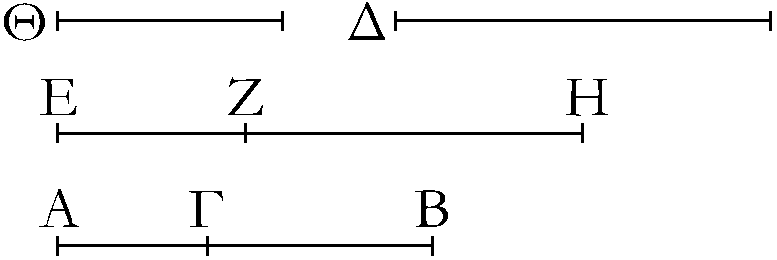
\includegraphics{Book10/fig049g.pdf}}

\gr{Ἐπεὶ γὰρ ἀνάπαλίν ἐστιν ὡξ ὁ ΒΑ ἀριθμὸξ πρὸξ τὸν ΑΓ,
ο<ύτωξ τὸ ἀπὸ τῆξ ΗΖ πρὸξ τὸ ἀπὸ τῆξ ΖΕ, μείζων δὲ ὁ
ΒΑ τοῦ ΑΓ, μεῖζον >άρα [καὶ] τὸ ἀπὸ τῆξ ΗΖ τοῦ ἀπὸ τῆξ
ΖΕ. >έστω τῶ| ἀπὸ τῆξ ΗΖ >ίσα τὰ ἀπὸ τῶν ΕΖ, Θ; ἀναστρέψαντι
>άρα ἐστὶν ὡξ ὁ ΑΒ πρὸξ τὸν ΒΓ, ο<ύτωξ τὸ ἀπὸ
τῆξ ΖΗ πρὸξ τὸ ἀπὸ τῆξ Θ. ἀλλ> ὁ ΑΒ πρὸξ τὸν ΒΓ
λόγον >έθει, <ὸν τετράγωνοξ ἀριθμὸξ πρὸξ τετράγωνον ἀριθμόν;
καὶ τὸ ἀπὸ τῆξ ΖΗ >άρα πρὸξ τὸ ἀπὸ τῆξ Θ λόγον
>έθει, <ὸν τετράγωνοξ ἀριθμὸξ πρὸξ τετράγωνον ἀριθμόν.
σύμμετροξ >άρα ἐστὶν ἡ ΖΗ τῆ| Θ μ\kern -.7pt  ήκει; <ώστε ἡ ΖΗ
τῆξ ΖΕ μεῖζον δύναται τῶ| ἀπὸ συμμέτρου ἑαυτῆ|. καί
εἰσι <ρηταὶ αἱ ΖΗ, ΖΕ δυνάμει μόνον σύμμετροι, καὶ τὸ ΕΖ
>έλασσον >όνομα τῆ| ἐκκειμένῃ <ρητῆ| σύμμετρόν
ἐστι τῆ| Δ μ\kern -.7pt  ήκει.}

\gr{Ἡ ΕΗ >άρα ἐκ δύο ὀνομάτων ἐστὶ δευτέρα; <όπερ >έδει δεῖχαι.
}}

\ParallelRText{
\begin{center}
{\large Proposition 49}
\end{center}

To find a second binomial (straight-line).

Let the two numbers $AC$ and $CB$ be laid down such that their sum $AB$
has to $BC$ the ratio which (some) square number (has) to (some)
square number, and does not have to $AC$ the ratio which (some)
square number (has) to (some) square number [Prop.~10.28~lem.~I]. And let the rational (straight-line) $D$ be laid down. And let $EF$ be commensurable in length with $D$.
$EF$ is thus a rational (straight-line).
So, let it also be contrived that as the number $CA$ (is) to $AB$,
so the (square) on $EF$ (is) to the (square) on $FG$ [Prop.~10.6~corr.]. Thus, the (square) on $EF$
is commensurable with the (square) on $FG$ [Prop.~10.6]. Thus, $FG$ is also a rational
(straight-line). And since the number $CA$ does not have to $AB$ the ratio
which (some) square number (has) to (some) square number, the
(square) on $EF$ does not have to the (square) on $FG$ the ratio
which (some) square number (has) to (some) square number either.
Thus, $EF$  is incommensurable in length with $FG$ [Prop.~10.9]. $EF$ and $FG$
are thus rational (straight-lines which are) commensurable in square only.
Thus, $EG$ is a binomial (straight-line) [Prop.~10.36]. So, we must show
that (it is) also a second (binomial straight-line).

% Removed epsf size command
\centerline{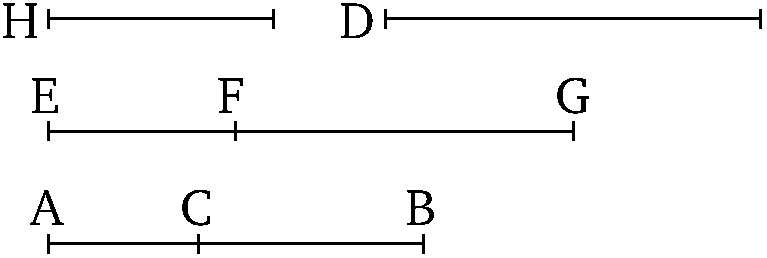
\includegraphics{Book10/fig049e.pdf}}

For since, inversely, as the number $BA$ is to $AC$, so the (square)
on $GF$ (is) to the (square) on $FE$ [Prop.~5.7 corr.],
and $BA$ (is) greater than $AC$, the (square) on $GF$ (is)
thus [also] greater than the (square) on $FE$ [Prop.~5.14]. Let (the sum of) the (squares) on $EF$ and $H$ be equal to the (square) on $GF$. Thus, via conversion, as 
$AB$ is to $BC$, so the (square) on $FG$ (is) to the (square) on $H$
[Prop.~5.19~corr.]. But, $AB$ has to $BC$ the
ratio which (some) square number (has) to (some) square number. Thus,
the (square) on $FG$ also has to the (square) on $H$ the ratio
which (some) square number (has) to (some) square number. Thus,
$FG$ is commensurable in length with $H$ [Prop.~10.9]. Hence, the square on $FG$ is
greater than (the square on) $FE$ by the (square) on (some straight-line)
commensurable in length with ($FG$). And $FG$ and $FE$ are rational (straight-lines which
are) commensurable in square only. And  the lesser term $EF$ is commensurable in length with the rational (straight-line) $D$ (previously)
laid down.

Thus, $EG$ is a second binomial (straight-line) [Def. 10.6].$^\dag$ (Which is) the very thing it
was required to show.}
\end{Parallel}
{\footnotesize\noindent $^\dag$ If the rational straight-line has unit length then the length of a second binomial straight-line
is  $k/\sqrt{1-k'^{\,2}}+k$. This, and the second apotome,
whose length is $k/\sqrt{1-k'^{\,2}}-k$ [Prop.~10.86],
are the roots of $x^2- (2\,k/\sqrt{1-k'^{\,2}})\,x+k^2\,[k'^{\,2}/(1-k'^{\,2})]=0$.}  

%%%%
%10.50
%%%%
\pdfbookmark[1]{Proposition 10.50}{pdf10.50}
\begin{Parallel}{}{}
\ParallelLText{
\begin{center}
{\large \ggn{50}.}
\end{center}\vspace*{-7pt}

\gr{Εὑρεῖν τὴν ἐκ δύο ὀνομάτων τρίτην.}

\gr{Ἐκκείσθωσαν δύο ἀριθμοὶ οἱ ΑΓ, ΓΒ, <ώστε τὸν συγκείμενον
ἐχ α\kern -.7pt  ὐτῶν τὸν ΑΒ πρὸξ μὲν τὸν ΒΓ λόγον >έθειν, <ὸν τετράγωνοξ
ἀριθμὸξ πρὸξ τετράγωνον ἀριθμόν, πρὸξ δὲ τὸν ΑΓ λόγον μ\kern -.7pt  ὴ
>έθειν, <ὸν τετράγωνοξ ἀριθμὸξ πρὸξ τετράγωνον ἀριθμόν. ἐκκείσθω
δέ τιξ καὶ >άλλοξ μ\kern -.5pt  ὴ τετράγωνοξ ἀριθμὸξ ὁ Δ, καὶ πρὸξ ἑκάτερον
τῶν ΒΑ, ΑΓ λόγον μ\kern -.3pt  ὴ ἐθέτω, <ὸν τετράγωνοξ ἀριθμὸξ πρὸξ τετράγωνον ἀριθμόν; καὶ ἐκκείσθω τιξ <ρητὴ εὐθεῖα ἡ Ε, καὶ
γεγονέτω ὡξ ὁ Δ πρὸξ τὸν ΑΒ, ο<ύτωξ τὸ ἀπὸ τῆξ Ε πρὸξ τὸ
ἀπὸ τῆξ ΖΗ; σύμμετρον >άρα ἐστὶ τὸ ἀπὸ τῆξ Ε τῶ| ἀπὸ
τῆξ ΖΗ. καί ἐστι <ρητὴ ἡ Ε; <ρητὴ >άρα ἐστὶ καὶ ἡ ΖΗ.
καὶ ἐπεὶ ὁ Δ πρὸξ τὸν ΑΒ λόγον οὐκ >έθει, <ὸν τετράγωνοξ
ἀριθμὸξ πρὸξ τετράγωνον ἀριθμόν, οὐδὲ τὸ ἀπὸ τῆξ Ε πρὸξ
τὸ ἀπὸ τῆξ ΖΗ λόγον >έθει, <ὸν τετράγωνοξ ἀριθμὸξ πρὸξ
τετράγωνον ἀριθμόν;
 ἀσύμμετροξ >άρα ἐστὶν ἡ Ε τῆ|
ΖΗ μ\kern -.7pt  ήκει. γεγονέτω δὴ πάλιν ὡξ ἡ ΒΑ ἀριθμὸξ πρὸξ τὸν ΑΓ,
ο<ύτωξ τὸ ἀπὸ τῆξ ΖΗ πρὸξ τὸ ἀπὸ τῆξ ΗΘ; σύμμετρον
>άρα ἐστὶ τὸ ἀπὸ τῆξ ΖΗ τῶ| ἀπὸ τῆξ ΗΘ. <ρητὴ δὲ ἡ ΖΗ;
<ρητὴ >άρα καὶ ἡ ΗΘ. καὶ ἐπεὶ ὁ ΒΑ πρὸξ τὸν ΑΓ λόγον οὐκ
>έθει, <ὸν τετράγωνοξ ἀριθμὸξ πρὸξ τετράγωνον ἀριθμόν, οὐδὲ
τὸ ἀπὸ τῆξ ΖΗ πρὸξ τὸ ἀπὸ τῆξ ΘΗ λόγον >έθει, <ὸν τετράγωνοξ
ἀριθμὸξ πρὸξ τετράγωνον ἀριθμόν;
ἀσύμμετροξ >άρα ἐστὶν ἡ ΖΗ τῆ| ΗΘ μ\kern -.7pt  ήκει. αἱ ΖΗ, ΗΘ
>άρα <ρηταί εἰσι δυνάμει μόνον σύμμετροι;
ἡ ΖΘ >άρα ἐκ δύο ὀνομάτων ἐστίν. λέγω δή, <ότι καὶ τρίτη.}\\~\\~\\~\\~\\~\\~\\

% Removed epsf size command
\centerline{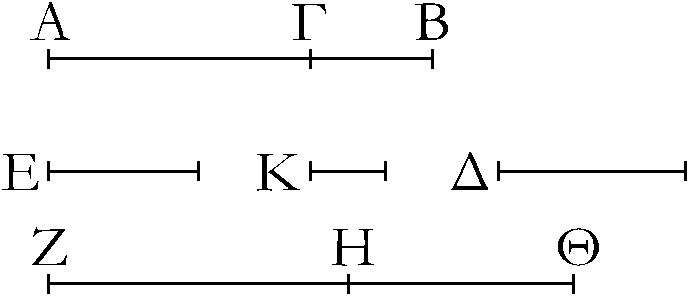
\includegraphics{Book10/fig050g.pdf}}

\gr{Ἐπεὶ γάρ ἐστιν ὡξ ὁ Δ πρὸξ τὸν ΑΒ, ο<ύτωξ τὸ ἀπὸ τῆξ
Ε πρὸξ τὸ ἀπὸ τῆξ ΖΗ, ὡξ δὲ ὁ ΒΑ πρὸξ τὸν ΑΓ, ο<ύτωξ
τὸ ἀπὸ τῆξ ΖΗ πρὸξ τὸ ἀπὸ τῆξ ΗΘ, δι> >ίσου >άρα
ἐστὶν ὡξ ὁ Δ πρὸξ τὸν ΑΓ, ο<ύτωξ τὸ ἀπὸ τῆξ Ε πρὸξ
τὸ ἀπὸ τῆξ ΗΘ. ὁ δὲ Δ πρὸξ τὸν ΑΓ λόγον οὐκ >έθει, <ὸν
τετράγωνοξ ἀριθμὸξ πρὸξ τετράγωνον ἀριθμόν; οὐδὲ τὸ ἀπὸ
τῆξ Ε >άρα πρὸξ τὸ ἀπὸ τῆξ ΗΘ λόγον >έθει, <ὸν τετράγωνοξ
ἀριθμὸξ πρὸξ τετράγωνον ἀριθμόν; ἀσύμμετροξ >άρα ἐστὶν ἡ Ε
τῆ| ΗΘ μ\kern -.7pt  ήκει. καὶ ἐπεί ἐστιν ὡξ ὁ ΒΑ πρὸξ τὸν ΑΓ, ο<ύτωξ
τὸ ἀπὸ τῆξ ΖΗ πρὸξ τὸ ἀπὸ τῆξ ΗΘ, μεῖζον
>άρα τὸ ἀπὸ τῆξ ΖΗ τοῦ ἀπὸ τῆξ ΗΘ. >έστω
ο>ῦν τῶ| ἀπὸ τῆξ ΖΗ >ίσα τὰ ἀπὸ τῶν ΗΘ, Κ; ἀναστρέψαντι
>άρα [ἐστὶν] ὡξ ὁ ΑΒ πρὸξ τὸν ΒΓ, ο<ύτωξ τὸ ἀπὸ τῆξ ΖΗ
πρὸξ τὸ ἀπὸ τῆξ Κ. ὁ δὲ ΑΒ πρὸξ τὸν ΒΓ λόγον >έθει,
<ὸν τετράγωνοξ ἀριθμὸξ πρὸξ τετράγωνον ἀριθμόν; καὶ
τὸ ἀπὸ τῆξ ΖΗ >άρα πρὸξ τὸ ἀπὸ τῆξ Κ λόγον >έθει, <ὸν
τετράγωνοξ ἀριθμὸξ πρὸξ τετράγωνον ἀριθμόν; σύμμετροξ
>άρα [ἐστὶν] ἡ ΖΗ τῆ| Κ μ\kern -.7pt  ήκει. ἡ ΖΗ >άρα τῆξ ΗΘ
μεῖζον δύναται τῶ| ἀπὸ συμμέτρου ἑαυτῆ|. καί εἰσιν αἱ
ΖΗ, ΗΘ <ρηταὶ δυνάμει μόνον σύμμετροι, καὶ οὐδετέρα α\kern -.5pt  ὐτῶν
σύμμετρόξ ἐστι τῆ| Ε μ\kern -.3pt  ήκει.}

\gr{Ἡ ΖΘ >άρα ἐκ δύο ὀνομάτων ἐστὶ τρίτη; <όπερ >έδει δεῖχαι.}}

\ParallelRText{
\begin{center}
{\large Proposition 50}
\end{center}

To find a third binomial (straight-line).

Let the two numbers $AC$ and $CB$ be laid down such that their sum
$AB$ has to $BC$ the ratio which (some) square number (has) to
(some) square number, and does not have to $AC$ the ratio which (some)
square number (has) to (some) square number. And let some other non-square number
$D$ also be laid down, and let it not have to each of $BA$ and $AC$ the
ratio which (some) square number (has) to (some) square number.
And let some rational straight-line $E$ be laid down, and let it be
contrived that as $D$ (is) to $AB$, so the (square) on $E$ (is) to
the (square) on $FG$ [Prop.~10.6~corr.]. Thus,
the (square) on $E$ is commensurable with the (square) on $FG$ [Prop.~10.6]. And $E$ is a rational (straight-line).
Thus, $FG$ is also a rational (straight-line). And since $D$ does not have to
$AB$ the ratio which (some) square number has to (some) square number,
the (square) on $E$ does not have to the (square) on $FG$ the ratio
which (some) square number (has) to (some) square number either.
$E$ is thus incommensurable in length with $FG$ [Prop.~10.9]. So, again, let it be contrived that
as the number $BA$ (is) to $AC$, so the (square) on  $FG$ (is) to the
(square) on $GH$ [Prop.~10.6~corr.]. Thus,
the (square) on $FG$ is commensurable with the (square) on $GH$
[Prop.~10.6]. And $FG$ (is) a rational (straight-line).
Thus, $GH$ (is) also a rational (straight-line). And since $BA$ does not have to $AC$ the ratio which (some) square number (has) to (some) square number, the (square) on $FG$  does not have to the (square) on $HG$
the ratio which (some) square number (has) to (some) square number either.
Thus, $FG$ is incommensurable in length with $GH$ [Prop.~10.9].  $FG$ and $GH$ are thus rational
(straight-lines which are) commensurable in square only. Thus,
$FH$ is a binomial (straight-line) [Prop.~10.36].
So, I say that (it is) also a third (binomial straight-line).

% Removed epsf size command
\centerline{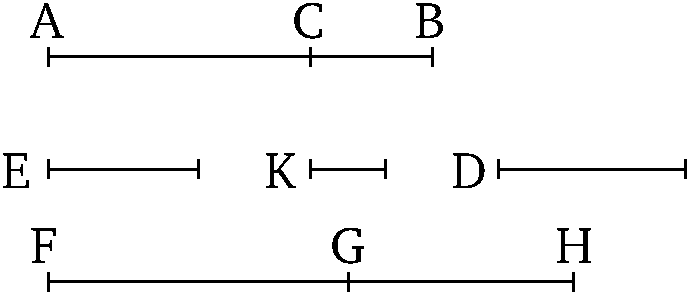
\includegraphics{Book10/fig050e.pdf}}

For since as $D$ is to $AB$, so the (square) on $E$ (is) to the (square)
on $FG$, and as $BA$ (is) to $AC$, so the (square) on $FG$ (is) to
the (square) on $GH$, thus, via equality, as $D$ (is) to $AC$, so the
(square) on $E$ (is) to the (square) on $GH$ [Prop.~5.22]. And $D$ does not have to $AC$ the
ratio which (some) square number (has) to (some) square number.
Thus, the (square) on $E$ does not have to the (square) on $GH$ the ratio
which (some) square number (has) to (some) square number either.
Thus, $E$ is incommensurable in length with $GH$ [Prop.~10.9].  And since as $BA$ is to $AC$,
so the (square) on $FG$ (is) to the (square) on $GH$, the (square) on 
$FG$ (is) thus greater than the (square) on $GH$ [Prop.~5.14]. Therefore, let (the sum of) the (squares)
on $GH$ and $K$
be equal to the (square) on $FG$. Thus, via
conversion, as $AB$ [is] to $BC$, so the (square) on $FG$ (is) to the
(square) on $K$ [Prop.~5.19~corr.]. And $AB$
has to $BC$ the ratio which (some) square number (has) to (some) square
number. Thus, the (square) on $FG$ also has to the (square) on $K$
the ratio which (some) square number (has) to (some) square number.
Thus,  $FG$ [is] commensurable in length with $K$ [Prop.~10.9]. Thus, the square on
$FG$ is greater than (the square on) $GH$ by the (square) on
(some straight-line) commensurable (in length) with ($FG$). And $FG$ and $GH$
are rational (straight-lines which are) commensurable in square only,
and neither of them is commensurable in length with $E$.

Thus, $FH$ is a third binomial (straight-line) [Def. 10.7].$^\dag$ (Which is) the very thing it
was required to show.}
\end{Parallel}
{\footnotesize\noindent$^\dag$ If the rational straight-line has unit length then the length of a third binomial straight-line
is  $k^{1/2}\,(1+\sqrt{1-k'^{\,2}})$. This, and the third apotome,
whose length is $k^{1/2}\,(1-\sqrt{1-k'^{\,2}})$ [Prop.~10.87],
are the roots of $x^2- 2\,k^{1/2}\,x+k\,k'^{\,2}=0$.}

%%%%
%10.51
%%%%
\pdfbookmark[1]{Proposition 10.51}{pdf10.51}
\begin{Parallel}{}{}
\ParallelLText{
\begin{center}
{\large \ggn{51}.}
\end{center}\vspace*{-7pt}

\gr{Εὑρεῖν τὴν ἐκ δύο ὀνομάτων τετάρτην.}

% Removed epsf size command
\centerline{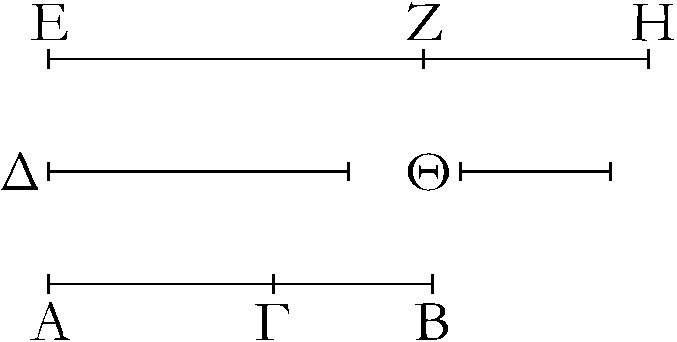
\includegraphics{Book10/fig051g.pdf}}

\gr{Ἐκκείσθωσαν δύο ἀριθμοὶ οἱ ΑΓ, ΓΒ, <ώστε τὸν ΑΒ πρὸξ τὸν
ΒΓ λόγον μ\kern -.7pt  ὴ >έθειν μ\kern -.7pt  ήτε μ\kern -.5pt  ὴν πρὸξ τὸν ΑΓ, <ὸν τετράγωνοξ
ἀριθμὸξ πρὸξ τετράγωνον ἀριθμόν. καὶ ἐκκείσθω <ρητὴ ἡ Δ,
καὶ τῆ| Δ σύμμετροξ >έστω μ\kern -.3pt  ήκει ἡ ΕΖ; <ρητὴ >άρα ἐστὶ
καὶ ἡ ΕΖ. καὶ γεγονέτω ὡξ ὁ ΒΑ ἀριθμὸξ πρὸξ τὸν ΑΓ,
ο<ύτωξ τὸ ἀπὸ τῆξ ΕΖ πρὸξ τὸ ἀπὸ τῆξ ΖΗ; σύμμετρον
>άρα ἐστὶ τὸ ἀπὸ τῆξ ΕΖ τῶ| ἀπὸ τῆξ ΖΗ; <ρητὴ >άρα ἐστὶ
καὶ ἡ ΖΗ. καὶ ἐπεὶ ὁ ΒΑ πρὸξ τὸν ΑΓ λόγον οὐκ >έθει,
<ὸν τετράγωνοξ ἀριθμὸξ πρὸξ τετράγωνον ἀριθμόν, οὐδὲ
τὸ ἀπὸ τῆξ ΕΖ  πρὸξ τὸ ἀπὸ τῆξ ΖΗ λόγον >έθει, <ὸν τετράγωνοξ
ἀριθμὸξ πρὸξ τετράγωνον ἀριθμόν; ἀσύμμετροξ >άρα ἐστὶν
ἡ ΕΖ τῆ| ΖΗ μ\kern -.7pt  ήκει. αἱ ΕΖ, ΖΗ >άρα <ρηταί εἰσι δυνάμει μόνον
σύμμετροι; <ώστε ἡ ΕΗ ἐκ δύο ὀνομάτων ἐστίν. λέγω δή,
<ότι καὶ τετάρτη.}

\gr{Ἐπεὶ γάρ ἐστιν ὡξ ὁ ΒΑ πρὸξ τὸν ΑΓ, ο<ύτωξ
τὸ ἀπὸ τῆξ ΕΖ πρὸξ τὸ ἀπὸ τῆξ ΖΗ [μείζων
δὲ ὁ ΒΑ τοῦ ΑΓ], μεῖζον >άρα τὸ ἀπὸ τῆξ ΕΖ τοῦ ἀπὸ
τῆξ ΖΗ. >έστω ο>ῦν τῶ| ἀπὸ τῆξ ΕΖ >ίσα τὰ ἀπὸ τῶν ΖΗ,
Θ; ἀναστρέψαντι >άρα ὡξ ὁ ΑΒ ἀριθμὸξ πρὸξ τὸν ΒΓ, ο<ύτωξ
τὸ ἀπὸ τῆξ ΕΖ πρὸξ τὸ ἀπὸ τῆξ Θ. ὁ δὲ ΑΒ πρὸξ τὸν ΒΓ
λόγον οὐκ >έθει, <ὸν τετράγωνοξ ἀριθμὸξ πρὸξ τετράγωνον
ἀριθμόν; οὐδ> >άρα τὸ ἀπὸ τῆξ ΕΖ πρὸξ τὸ ἀπὸ τῆξ Θ
λόγον >έθει, <ὸν τετράγωνοξ ἀριθμὸξ πρὸξ τετράγωνον ἀριθμόν.
ἀσύμμετροξ >άρα ἐστὶν ἡ ΕΖ τῆ| Θ μ\kern -.7pt  ήκει; ἡ ΕΖ >άρα τῆξ
ΗΖ μεῖζον δύναται τῶ| ἀπὸ ἀσυμμέτρου ἑαυτῆ|. καί
εἰσιν αἱ ΕΖ, ΖΗ <ρηταὶ δυνάμει μόνον σύμμετροι, καὶ
ἡ ΕΖ τῆ| Δ σύμμετρόξ ἐστι μ\kern -.7pt  ήκει.}

\gr{Ἡ ΕΗ >άρα ἐκ δύο ὀνομάτων ἐστὶ τετάρτη; <όπερ
>έδει δεῖχαι.}}

\ParallelRText{
\begin{center}
{\large Proposition 51}
\end{center}

To find a fourth binomial (straight-line).

% Removed epsf size command
\centerline{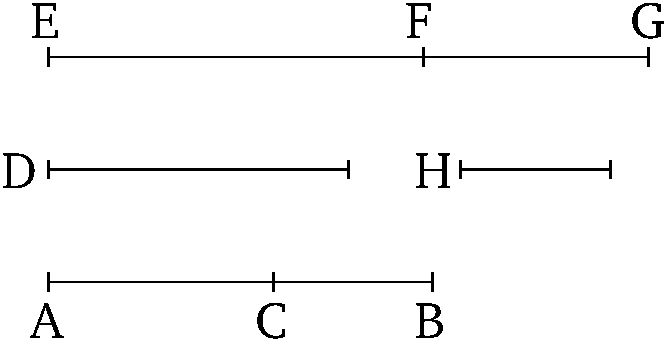
\includegraphics{Book10/fig051e.pdf}}

Let the two numbers $AC$ and $CB$ be laid down such that $AB$ does not have to $BC$,  or to $AC$ either, the ratio which (some) square number
(has) to (some) square number [Prop.~10.28~lem.~I].
And let the rational (straight-line) $D$ be laid down. And let $EF$ be
commensurable in length with $D$. Thus, $EF$ is also a rational (straight-line). And let it be contrived that as the number $BA$ (is) to
$AC$, so the (square) on $EF$ (is) to the (square) on $FG$ [Prop.~10.6~corr.]. Thus, the (square) on $EF$
is commensurable with the (square) on $FG$ [Prop.~10.6]. Thus, $FG$ is also a rational (straight-line). And since $BA$ does not have to $AC$ the ratio which (some)
square number (has) to (some) square number,  the (square) on $EF$
does not have to the (square) on $FG$ the ratio which (some) square number
(has) to (some) square number either. Thus, $EF$ is incommensurable in length with $FG$ [Prop.~10.9]. Thus, $EF$ and
$FG$ are rational (straight-lines which are) commensurable in square only.
Hence, $EG$ is a binomial (straight-line) [Prop.~10.36]. So, I say that (it is) also
a fourth (binomial straight-line).

For since as $BA$ is to $AC$, so the (square) on $EF$ (is) to the (square) on
$FG$ [and $BA$ (is) greater than $AC$], the (square) on $EF$ (is) thus
greater than the (square) on $FG$ [Prop.~5.14]. Therefore, let (the sum of) the squares on
$FG$ and $H$ be equal to the (square) on $EF$. Thus, via conversion,
as the number $AB$ (is) to $BC$, so the (square) on $EF$ (is) to the
(square) on $H$ [Prop.~5.19~corr.]. And $AB$
does not have to $BC$ the ratio which (some) square number (has) to (some)
square number. Thus, the (square) on $EF$ does not have to the
(square) on $H$ the ratio which (some) square number (has) to (some) square
number either. Thus, $EF$ is incommensurable in length with $H$ [Prop.~10.9]. Thus, the square on $EF$ is greater than (the square on) $GF$ by the (square) on (some straight-line)
incommensurable (in length) with ($EF$). And $EF$ and $FG$ are rational (straight-lines which are) commensurable in square only.  And $EF$ is commensurable
in length with $D$.

Thus, $EG$ is a fourth binomial (straight-line) [Def. 10.8].$^\dag$ (Which is) the very thing
it was required to show.}
\end{Parallel}
{\footnotesize\noindent $^\dag$ If the rational straight-line has unit length then the length of a fourth binomial straight-line
is  $k\,(1+1/\sqrt{1+k'})$. This, and the fourth apotome,
whose length is $k\,(1-1/\sqrt{1+k'})$ [Prop.~10.88],
are the roots of $x^2- 2\,k\,x+k^2\,k'/(1+k')=0$.}

%%%%
%10.52
%%%%
\pdfbookmark[1]{Proposition 10.52}{pdf10.52}
\begin{Parallel}{}{}
\ParallelLText{
\begin{center}
{\large \ggn{52}.}
\end{center}\vspace*{-7pt}

\gr{Εὑρεῖν τὴν ἐκ δύο ὀνομάτων πέμπτην.}

% Removed epsf size command
\centerline{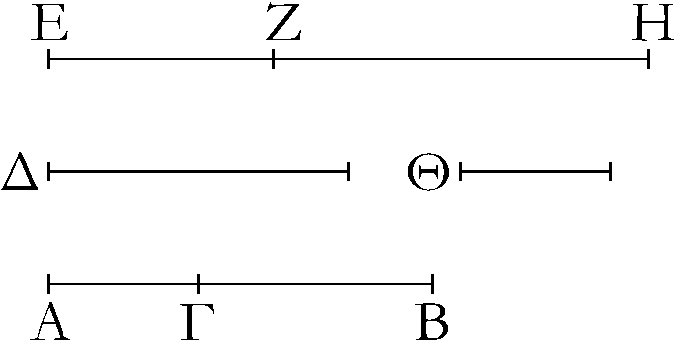
\includegraphics{Book10/fig052g.pdf}}

\gr{Ἐκκείσθωσαν δύο ἀριθμοὶ οἱ ΑΓ, ΓΒ, <ώστε τὸν ΑΒ πρὸξ ἑκάτερον
α\kern -.7pt  ὐτῶν λόγον μ\kern -.7pt  ὴ >έθειν, <ὸν τετράγωνοξ ἀριθμὸξ πρὸξ τετράγωνον
ἀριθμόν, καὶ ἐκκείσθω <ρητή τιξ εὐθεῖα ἡ Δ, καὶ τῆ| Δ σύμμετροξ
>έστω [μ\kern -.5pt  ήκει] ἡ ΕΖ; <ρητὴ >άρα ἡ ΕΖ. καὶ γεγονέτω ὡξ ὁ ΓΑ
πρὸξ τὸν ΑΒ, ο<ύτωξ τὸ ἀπὸ τῆξ ΕΖ πρὸξ τὸ ἀπὸ τῆξ ΖΗ.
ὁ δὲ ΓΑ πρὸξ τὸν ΑΒ λόγον οὐκ >έθει, <ὸν τετράγωνοξ ἀριθμὸξ
πρὸξ τετράγωνον ἀριθμόν; οὑδὲ τὸ ἀπὸ τῆξ ΕΖ >άρα πρὸξ
τὸ ἀπὸ τῆξ ΖΗ λόγον >έθει, <ὸν τετράγωνοξ ἀριθμὸξ πρὸξ
τετράγωνον ἀριθμόν. αἱ ΕΖ, ΖΗ >άρα <ρηταί εἰσι δυνάμει
μόνον σύμμετροι; ἐκ δύο >άρα ὀνομάτων ἐστὶν ἡ ΕΗ. λέγω δή, <ότι καὶ πέμπτη.}

\gr{Ἐπεὶ γάρ ἐστιν ὡξ ὁ ΓΑ πρὸξ τὸν ΑΒ, ο<ύτωξ τὸ ἀπὸ τῆξ ΕΖ
πρὸξ τὸ ἀπὸ τῆξ ΖΗ, ἀνάπαλιν ὡξ ὁ ΒΑ πρὸξ τὸν ΑΓ, ο<ύτωξ
τὸ ἀπὸ τῆξ ΖΗ πρὸξ τὸ ἀπὸ τῆξ ΖΕ; μεῖζον >άρα τὸ ἀπὸ
τῆξ ΗΖ τοῦ ἀπὸ τῆξ ΖΕ. >έστω ο>ῦν τῶ| ἀπὸ τῆξ
ΗΖ >ίσα τὰ ἀπὸ τῶν ΕΖ, Θ; ἀναστρέψαντι >άρα ἐστὶν ὡξ ὁ ΑΒ
ἀριθμὸξ πρὸξ τὸν ΒΓ, ο<ύτωξ τὸ ἀπὸ τῆξ ΗΖ πρὸξ τὸ
ἀπὸ τῆξ Θ. ὁ δὲ ΑΒ πρὸξ τὸν ΒΓ λόγον οὐκ >έθει, <ὸν
τετράγωνοξ ἀριθμὸξ πρὸξ τετράγωνον ἀριθμόν; οὐδ> >άρα τὸ
ἀπὸ τῆξ ΖΗ πρὸξ τὸ ἀπὸ τῆξ Θ λόγον
>έθει, <ὸν τετράγωνοξ ἀριθμὸξ πρὸξ τετράγωνον ἀριθμόν.
ἀσύμμετροξ >άρα ἐστὶν ἡ ΖΗ τῆ| Θ
μ\kern -.7pt  ήκει; <ώστε ἡ ΖΗ τῆξ ΖΕ μεῖζον δύναται τῶ| ἀπὸ ἀσυμμέτρου
ἑαυτῆ|. καί εἰσιν αἱ ΗΖ, ΖΕ <ρηταὶ δυνάμει μόνον σύμμετροι,
καὶ τὸ ΕΖ >έλαττον >όνομα σύμμετρόν ἐστι τῆ| ἐκκειμένῃ
<ρητῆ| τῆ| Δ μ\kern -.7pt  ήκει.}

\gr{Ἡ ΕΗ >άρα ἐκ δύο ὀνομάτων ἐστὶ πέμπτη; <όπερ
>έδει δεῖχαι.}}

\ParallelRText{
\begin{center}
{\large Proposition 52}
\end{center}

To find a fifth binomial straight-line.

% Removed epsf size command
\centerline{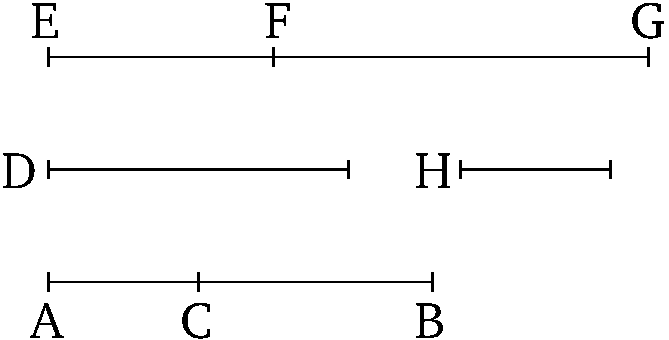
\includegraphics{Book10/fig052e.pdf}}

Let the two numbers $AC$ and $CB$ be laid down such that $AB$ does
not have to either of them the ratio which (some) square number (has)
to (some) square number [Prop.~10.38~lem.]. And
let some rational straight-line $D$ be laid down. And let $EF$ be
commensurable [in length] with $D$. Thus, $EF$ (is) a rational (straight-line).
And let it be contrived that as $CA$ (is) to $AB$, so the (square) on
$EF$ (is) to the (square) on $FG$ [Prop.~10.6~corr.].
 And $CA$ does not have to $AB$ the ratio which (some)
 square number (has) to (some) square number. Thus, the (square) on
 $EF$ does not have to the (square) on $FG$ the ratio which (some)
 square number (has) to (some) square number either. Thus, $EF$ and
 $FG$ are rational (straight-lines which are) commensurable in square only
 [Prop.~10.9].  Thus, $EG$ is a binomial (straight-line) [Prop.~10.36]. So, I say that (it is) also
 a fifth (binomial straight-line).
 
 For since as $CA$ is to $AB$, so the (square) on $EF$ (is) to the (square)
 on $FG$, inversely, as $BA$ (is) to $AC$, so the (square) on $FG$ (is)
 to the (square) on $FE$ [Prop.~5.7~corr.]. Thus,
 the (square) on $GF$ (is) greater than the (square) on $FE$ [Prop.~5.14]. Therefore, let (the sum of) the (squares)
 on $EF$ and $H$ be equal to the (square) on $GF$. Thus, via conversion, 
 as the number $AB$ is to $BC$, so the (square) on $GF$ (is) to
 the (square) on $H$ [Prop.~5.19~corr.]. 
 And $AB$ does not have to $BC$ the ratio which (some) square number
 (has) to (some) square number. Thus, the (square) on $FG$ does not have
 to the (square) on $H$ the ratio which (some) square number (has) to
 (some) square number either. Thus, $FG$ is incommensurable in length
 with $H$ [Prop.~10.9]. Hence, the square on $FG$
 is greater than (the square on) $FE$ by the (square) on (some straight-line)
 incommensurable (in length) with ($FG$). And $GF$ and $FE$ are rational (straight-lines
 which are) commensurable in square only. And the lesser term $EF$ is commensurable in length with the  rational (straight-line previously)  laid down, $D$.
 
 Thus, $EG$ is a fifth binomial (straight-line).$^\dag$  (Which is) the very thing it
 was required to show.}
\end{Parallel}
{\footnotesize\noindent $^\dag$ If the rational straight-line has unit length then the length of a fifth binomial straight-line
is  $k\,(\sqrt{1+k'}+1)$. This, and the fifth apotome,
whose length is $k\,(\sqrt{1+k'}-1)$ [Prop.~10.89],
are the roots of $x^2- 2\,k\,\sqrt{1+k'}\,x+k^2\,k'=0$.}
 
%%%%
%10.53
%%%%
\pdfbookmark[1]{Proposition 10.53}{pdf10.53}
\begin{Parallel}{}{}
\ParallelLText{
\begin{center}
{\large \ggn{53}.}
\end{center}\vspace*{-7pt}

\gr{Εὑρεῖν τὴν ἐκ δύο ὀνομάτων <έκτην.}

% Removed epsf size command
\centerline{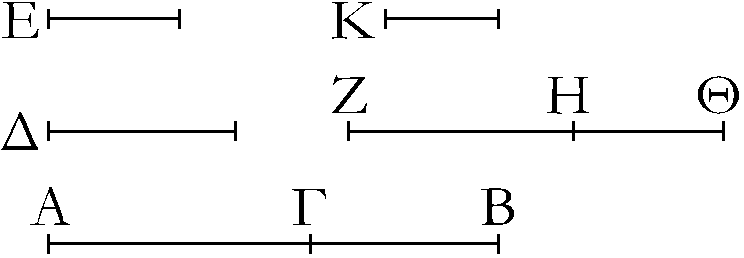
\includegraphics{Book10/fig053g.pdf}}

\gr{Ἐκκείσθωσαν δύο ἀριθμοὶ οἱ ΑΓ, ΓΒ, <ώστε τὸν ΑΒ πρὸξ ἑκάτερον
α\kern -.7pt  ὐτῶν λόγον μ\kern -.7pt  ὴ >έθειν, <ὸν τετράγωνοξ ἀριθμὸξ πρὸξ τετράγωνον
ἀριθμόν; >έστω δὲ καὶ <έτεροξ ἀριθμὸξ ὁ Δ μ\kern -.5pt  ὴ τετράγωνοξ >ὼν
μ\kern -.3pt  ηδὲ πρὸξ ἑκάτερον τῶν ΒΑ, ΑΓ λόγον >έθων, <ὸν τετράγωνοξ
ἀριθμὸξ πρὸξ τετράγωνον ἀριθμόν; καὶ ἐκκείσθω τιξ
<ρητὴ εὐθεῖα ἡ Ε, καὶ γεγονέτω ὡξ ὁ Δ πρὸξ τὸν ΑΒ, ο<ύτωξ
τὸ ἀπὸ τῆξ Ε πρὸξ τὸ ἀπὸ τῆξ ΖΗ; σύμμετρον >άρα τὸ ἀπὸ
τῆξ Ε τῶ| ἀπὸ τῆξ ΖΗ. καί ἐστι <ρητὴ ἡ Ε; <ρητὴ >άρα καὶ ἡ ΖΗ. καὶ ἐπεὶ οὐκ >έθει ὁ Δ πρὸξ τὸν ΑΒ λόγον, <ὸν τετράγωνοξ
ἀριθμὸξ πρὸξ τετράγωνον ἀριθμόν, οὐδὲ τὸ ἀπὸ τῆξ Ε >άρα πρὸξ τὸ ἀπὸ τῆξ ΖΗ λόγον >έθει, <ὸν τετράγωνοξ ἀριθμὸξ πρὸξ τετράγωνον ἀριθμόν; ἀσύμμετροξ >άρα ἡ Ε τῆ| ΖΗ μ\kern -.7pt  ήκει. γεγονέτω
δὴ πάλιν ὡξ ὁ ΒΑ πρὸξ τὸν ΑΓ, ο<ύτωξ τὸ ἀπὸ τῆξ ΖΗ
πρὸξ τὸ ἀπὸ τῆξ ΗΘ. σύμμετρον >άρα τὸ ἀπὸ τῆξ ΖΗ τῶ|
ἀπὸ τῆξ ΘΗ. <ρητὸν >άρα τὸ ἀπὸ τῆξ ΘΗ; <ρητὴ >άρα ἡ ΘΗ. καὶ
ἐπεὶ ὁ ΒΑ πρὸξ τὸν ΑΓ λόγον οὐκ >έθει, <ὸν τετράγωνοξ
ἀριθμὸξ πρὸξ τετράγωνον ἀριθμόν, οὐδὲ τὸ ἀπὸ τῆξ ΖΗ πρὸξ
τὸ ἀπὸ τῆξ ΗΘ λόγον >έθει, <ὸν τετράγωνοξ ἀριθμὸξ
πρὸξ τετράγωνον ἀριθμόν; ἀσύμμετροξ >άρα ἐστὶν ἡ ΖΗ
τῆ| ΗΘ μ\kern -.7pt  ήκει. αἱ ΖΗ, ΗΘ >άρα <ρηταί εἰσι
δυνάμει μόνον σύμμετροι; ἐκ δύο >άρα ὀνομάτων ἐστὶν ἡ ΖΘ. δεικτέον δή, <ότι καὶ <έκτη.}

\gr{Ἐπεὶ γάρ ἐστιν ὡξ ὁ Δ πρὸξ τὸν ΑΒ, ο<ύτωξ τὸ ἀπὸ τῆξ Ε πρὸξ
τὸ ἀπὸ τῆξ ΖΗ, >έστι δὲ καὶ ὡξ ὁ ΒΑ πρὸξ τὸν ΑΓ, ο<ύτωξ
τὸ ἀπὸ τῆξ ΖΗ πρὸξ τὸ ἀπὸ τῆξ ΗΘ, δι> >ίσου >άρα ἐστὶν
ὡξ ὁ Δ πρὸξ τὸν ΑΓ, ο<ύτωξ τὸ ἀπὸ τῆξ Ε πρὸξ τὸ ἀπὸ
τῆξ ΗΘ. ὁ δὲ Δ πρὸξ τὸν ΑΓ λόγον οὐκ >έθει, <ὸν τετράγωνοξ
ἀριθμὸξ πρὸξ τετράγωνον ἀριθμόν; οὐδὲ τὸ ἀπὸ τῆξ
Ε >άρα πρὸξ τὸ ἀπὸ τῆξ ΗΘ λόγον >έθει, <ὸν τετράγωνοξ
ἀριθμὸξ πρὸξ τετράγωνον ἀριθμόν;
ἀσύμμετροξ >άρα ἐστὶν
ἡ Ε τῆ| ΗΘ μ\kern -.7pt  ήκει. ἐδείθθη δὲ καὶ τῆ| ΖΗ ἀσύμμετροξ;
ἑκατέρα >άρα τῶν ΖΗ, ΗΘ ἀσύμμετρόξ ἐστι τῆ| Ε μ\kern -.7pt  ήκει.
καὶ ἐπεί ἐστιν ὡξ ὁ ΒΑ πρὸξ τὸν ΑΓ, ο<ύτωξ τὸ ἀπὸ
τῆξ ΖΗ πρὸξ τὸ ἀπὸ τῆξ ΗΘ, μεῖζον >άρα τὸ ἀπὸ τῆξ ΖΗ
τοῦ ἀπὸ τῆξ ΗΘ. >έστω ο>ῦν τῶ| ἀπὸ [τῆξ] ΖΗ >ίσα
τὰ ἀπὸ τῶν ΗΘ, Κ; ἀναστρέψαντι >άρα ὡξ ὁ ΑΒ πρὸξ ΒΓ, ο<ύτωξ
τὸ ἀπὸ ΖΗ πρὸξ τὸ ἀπὸ τῆξ Κ. ὁ δὲ ΑΒ πρὸξ τὸν ΒΓ λόγον
οὐκ >έθει, <ὸν τετράγωνοξ ἀριθμὸξ πρὸξ τετράγωνον ἀριθμόν; <ώστε
οὐδὲ τὸ ἀπὸ ΖΗ πρὸξ τὸ ἀπὸ τῆξ Κ λόγον >έθει, <ὸν
τετράγωνοξ ἀριθμὸξ πρὸξ τετράγωνον ἀριθμόν. ἀσύμμετροξ >άρα
ἐστὶν ἡ ΖΗ τῆ| Κ μ\kern -.5pt  ήκει; ἡ ΖΗ >άρα τῆξ ΗΘ μεῖζον δύναται
τῶ| ἀπὸ ἀσυμμέτρου ἑαυτῆ|. καί εἰσιν αἱ ΖΗ, ΗΘ <ρηταὶ δυνάμει
μόνον σύμμετροι, καὶ οὐδετέρα α\kern -.3pt  ὐτῶν σύμμετρόξ ἐστι μ\kern -.7pt  ήκει
τῆ| ἐκκειμένῃ <ρητῃ τῆ| Ε.}

\gr{Ἡ ΖΘ >άρα ἐκ δύο ὀνομάτων ἐστὶν <έκτη; <όπερ >έδει δεῖχαι.}}

\ParallelRText{
\begin{center}
{\large Proposition 53}
\end{center}

To find a sixth binomial (straight-line).

% Removed epsf size command
\centerline{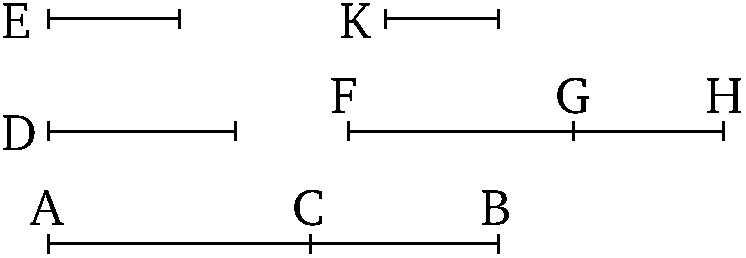
\includegraphics{Book10/fig053e.pdf}}

Let the two numbers $AC$ and $CB$ be laid down such that $AB$ does
not have to each of them the ratio which (some) square number (has) to (some) square number.  And let $D$  also be another number, which is not
square, and does not have to each of $BA$ and $AC$ the ratio which (some)
square number (has) to (some) square number either [Prop.~10.28~lem.~I]. And let some rational straight-line $E$ be laid down. And let it be contrived that as $D$ (is) to
$AB$, so the (square) on $E$ (is) to the (square) on $FG$ [Prop.~10.6~corr.].  Thus, the (square) on $E$
(is) commensurable with the (square) on $FG$ [Prop.~10.6]. And $E$ is rational. Thus, $FG$
(is) also rational.  And since $D$ does not have to $AB$ the ratio
which (some) square number (has) to (some) square number, the (square) on $E$ thus does not have to the (square) on $FG$ the ratio which (some) square number (has) to (some) square number either. Thus, $E$ (is) incommensurable in length with $FG$ [Prop.~10.9].
So, again, let it have be contrived that as $BA$ (is) to $AC$, so the (square)
on $FG$ (is) to the (square) on $GH$ [Prop.~10.6~corr.]. The (square) on $FG$ (is)
thus commensurable with the (square) on $HG$ [Prop.~10.6].
 The (square) on $HG$ (is) thus rational.  Thus, $HG$ (is) rational. And since $BA$ does not have to
$AC$ the ratio which (some) square number (has) to (some) square number,
the (square) on $FG$ does not have to the (square) on $GH$ the
ratio which (some) square number (has) to (some) square number either.
Thus, $FG$ is incommensurable in length with $GH$ [Prop.~10.9]. Thus, $FG$ and $GH$ are rational (straight-lines which are) commensurable in square only. Thus, $FH$
is a binomial (straight-line) [Prop.~10.36]. So,
we must show that (it is) also a sixth (binomial straight-line).

For since as $D$ is to $AB$, so the (square) on $E$ (is) to the (square) on
$FG$, and also as $BA$ is to $AC$, so the (square) on $FG$ (is) to
the (square) on $GH$, thus, via equality, as $D$ is to $AC$, so
the (square) on $E$ (is) to the (square) on $GH$ [Prop.~5.22]. And $D$ does not have to $AC$ the
ratio which (some) square number (has) to (some) square number.  Thus, 
the (square) on $E$ does not have to the (square) on $GH$ the ratio
which (some) square number (has) to (some) square number either. $E$
is thus incommensurable in length with $GH$ [Prop.~10.9]. And ($E$) was also shown (to be)
incommensurable (in length) with $FG$.  Thus,  $FG$ and $GH$ are
each incommensurable in length with $E$. And since as $BA$ is to $AC$, 
so the (square) on $FG$ (is) to the (square) on $GH$, the (square) on $FG$ (is) thus greater than the (square) on $GH$ [Prop.~5.14]. Therefore, let (the sum of) the
(squares) on $GH$ and $K$ be equal to the (square) on $FG$. Thus,
via conversion, as $AB$ (is) to $BC$,
 so the (square) on $FG$ (is) to the
(square) on $K$ [Prop.~5.19~corr.].  And $AB$ does not
have to $BC$ the ratio which (some) square number (has) to (some) square number. Hence, the (square) on $FG$ does not have to the (square) on
$K$ the ratio which (some) square number (has) to (some) square number either. Thus, $FG$ is incommensurable in length with $K$ [Prop.~10.9]. The square on $FG$ is thus
greater than (the square on) $GH$ by the (square) on (some straight-line which is) incommensurable (in length) with ($FG$). And  $FG$ and $GH$ are rational
(straight-lines which are) commensurable in square only, and neither of them
is commensurable in length with the  rational (straight-line) $E$ (previously)
laid down.

Thus, $FH$ is a  sixth binomial (straight-line) [Def. 10.10].$^\dag$ (Which is) the very thing it was required to show.}
\end{Parallel}
{\footnotesize\noindent$^\dag$ If the rational straight-line has unit length then the length of a sixth binomial straight-line
is  $\sqrt{k}+\sqrt{k'}$. This, and the sixth apotome,
whose length is $\sqrt{k}-\sqrt{k'}$ [Prop.~10.90],
are the roots of $x^2- 2\,\sqrt{k}\,x+(k-k')=0$.}

%%%%
%10.53lem
%%%%
\begin{Parallel}{}{}
\ParallelLText{

\begin{center}
{\large \gr{Λῆμμα}.}
\end{center}\vspace*{-7pt}

\gr{>'Εστω δύο τετράγωνα τὰ ΑΒ, ΒΓ καὶ κείσθωσαν <ώστε ἐπ> εὐθείαξ  ε>ῖναι τὴν ΔΒ τῆ| ΒΕ; ἐπ> εὐθείαξ >άρα
ἐστὶ καὶ ἡ ΖΒ τῆ| ΒΗ. καὶ συμπεπληρώσθω τὸ ΑΓ παραλληλόγραμμον;
λέγω, <ότι τετράγωνόν ἐστι τὸ ΑΓ, καὶ <ότι τῶν ΑΒ, ΒΓ μέσον ἀνάλογόν ἐστι τὸ ΔΗ, καὶ >έτι τῶν ΑΓ, ΓΒ μέσον ἀνάλογόν ἐστι
τὸ ΔΓ.}

\gr{Ἐπεὶ γὰρ >ίση ἐστὶν ἡ μὲν ΔΒ τῆ| ΒΖ, ἡ δὲ ΒΕ τῆ| ΒΗ, <όλη
>άρα ἡ ΔΕ <όλῃ τῆ| ΖΗ ἐστιν >ίση. ἀλλ> ἡ μὲν ΔΕ ἑκατέρᾳ
τῶν ΑΘ, ΚΓ ἐστιν >ίση, ἡ δὲ ΖΗ ἑκατέρᾳ τῶν ΑΚ, ΘΓ ἐστιν >ίση;
καὶ ἑκατέρα >άρα τῶν ΑΘ, ΚΓ ἑκατέρᾳ τῶν ΑΚ, ΘΓ ἐστιν >ίση.
ἰσόπλευρον >άρα ἐστὶ τὸ ΑΓ παραλληλόγραμμον; >έστι δὲ καὶ
ὀρθογώνιον; τετράγωνον >άρα ἐστὶ τὸ ΑΓ.}

\gr{Καὶ ἐπεὶ ἐστιν ὡξ ἡ ΖΒ πρὸξ τὴν ΒΗ, ο<ύτωξ ἡ
ΔΒ πρὸξ τὴν ΒΕ, ἀλλ> ὡξ μὲν ἡ ΖΒ πρὸξ τὴν ΒΗ, ο<ύτωξ τὸ ΑΒ
πρὸξ τὸ ΔΗ, ὡξ δὲ ἡ ΔΒ πρὸξ τὴν ΒΕ, ο<ύτωξ τὸ ΔΗ πρὸξ
τὸ ΒΓ, καὶ ὡξ >άρα τὸ ΑΒ πρὸξ τὸ ΔΗ, ο<ύτωξ τὸ ΔΗ πρὸξ τὸ
ΒΓ. τῶν ΑΒ, ΒΓ >άρα μέσον ἀνάλογόν ἐστι τὸ ΔΗ.}

\gr{Λέγω δή, <ότι καὶ τῶν ΑΓ, ΓΒ μέσον ἀνάλογόν [ἐστι] τὸ ΔΓ.}

% Removed epsf size command
\centerline{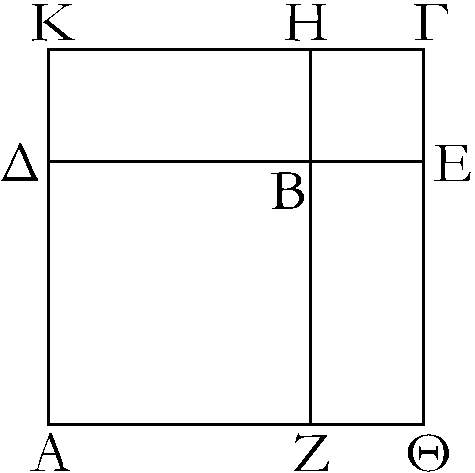
\includegraphics{Book10/fig053ag.pdf}}

\gr{Ἐπεὶ γάρ ἐστιν ὡξ ἡ ΑΔ πρὸξ τὴν ΔΚ, ο<ύτωξ ἡ ΚΗ πρὸξ
τὴν ΗΓ; >ίση γάρ [ἐστιν] ἑκατέρα ἑκατέρᾳ; καὶ συνθέντι ὡξ ἡ ΑΚ
πρὸξ ΚΔ, ο<ύτωξ ἡ ΚΓ
πρὸξ ΓΗ, ἀλλ> ὡξ μὲν ἡ ΑΚ πρὸξ ΚΔ, ο<ύτωξ
τὸ ΑΓ πρὸξ τὸ ΓΔ, ὡξ δὲ ἡ ΚΓ πρὸξ ΓΗ, ο<ύτωξ τὸ ΔΓ πρὸξ
ΓΒ, καὶ ὡξ >άρα τὸ ΑΓ πρὸξ ΔΓ, ο<ύτωξ τὸ ΔΓ πρὸξ τὸ ΒΓ. τῶν ΑΓ, ΓΒ >άρα μέσον ἀνάλογόν ἐστι τὸ ΔΓ; <ὰ προέκειτο
δεῖχαι.}}

\ParallelRText{
\begin{center}
{\large Lemma}
\end{center}

Let $AB$ and $BC$ be two squares, and let them
be laid down such that $DB$ is straight-on to $BE$. $FB$ is, thus, also
straight-on to $BG$. And let the parallelogram $AC$ be completed.
I say that $AC$ is a square, and that $DG$ is  the mean proportional to $AB$ and
$BC$, and, moreover,  $DC$ is the mean proportional to $AC$ and $CB$.

For since $DB$ is equal to $BF$, and $BE$ to $BG$, the whole of $DE$
is thus equal to the whole of $FG$. But $DE$ is equal to each of $AH$
and $KC$, and $FG$ is equal to each of $AK$ and $HC$ [Prop.~1.34]. Thus, $AH$ and $KC$ are also 
equal to  $AK$ and $HC$, respectively. Thus, the parallelogram $AC$
is equilateral. And (it is) also right-angled. Thus, $AC$ is a square.

And since as $FB$ is to $BG$, so $DB$ (is) to $BE$, but as $FB$
(is) to $BG$, so $AB$ (is) to $DG$, and as $DB$ (is) to $BE$, so
$DG$ (is) to $BC$ [Prop.~6.1], thus also as $AB$ (is) to $DG$, so $DG$  (is) to $BC$ [Prop.~5.11]. Thus, $DG$ is the mean proportional
to $AB$ and $BC$.

So I also say that $DC$ [is] the mean proportional to $AC$ and $CB$.

% Removed epsf size command
\centerline{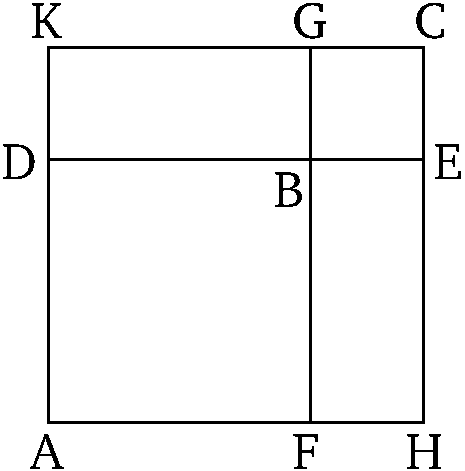
\includegraphics{Book10/fig053ae.pdf}}

For since as $AD$ is to $DK$, so $KG$ (is) to $GC$. For [they are]  respectively equal. And, via composition, as $AK$ (is) to $KD$, so
$KC$ (is) to $CG$ [Prop.~5.18]. But as
$AK$ (is) to $KD$, so $AC$ (is) to $CD$, and as $KC$ (is) to $CG$,
so $DC$ (is) to $CB$ [Prop.~6.1]. Thus, also, as $AC$ (is) to $DC$, so
$DC$ (is) to $BC$ [Prop.~5.11]. Thus, $DC$ is the mean proportional to $AC$ and
$CB$. Which (is the very thing) it was prescribed to show.}
\end{Parallel}

%%%%
%10.54
%%%%
\pdfbookmark[1]{Proposition 10.54}{pdf10.54}
\begin{Parallel}{}{}
\ParallelLText{
\begin{center}
{\large \ggn{54}.}
\end{center}\vspace*{-7pt}

\gr{Ἐὰν θωρίον περιέθηται ὑπὸ <ρητῆξ καὶ τῆξ ἐκ δύο ὀνομάτων
πρώτηξ, ἡ τὸ θωρίον δυναμένη >άλογόξ ἐστιν ἡ καλουμένη ἐκ δύο
ὀνομάτων.}

% Removed epsf size command
\centerline{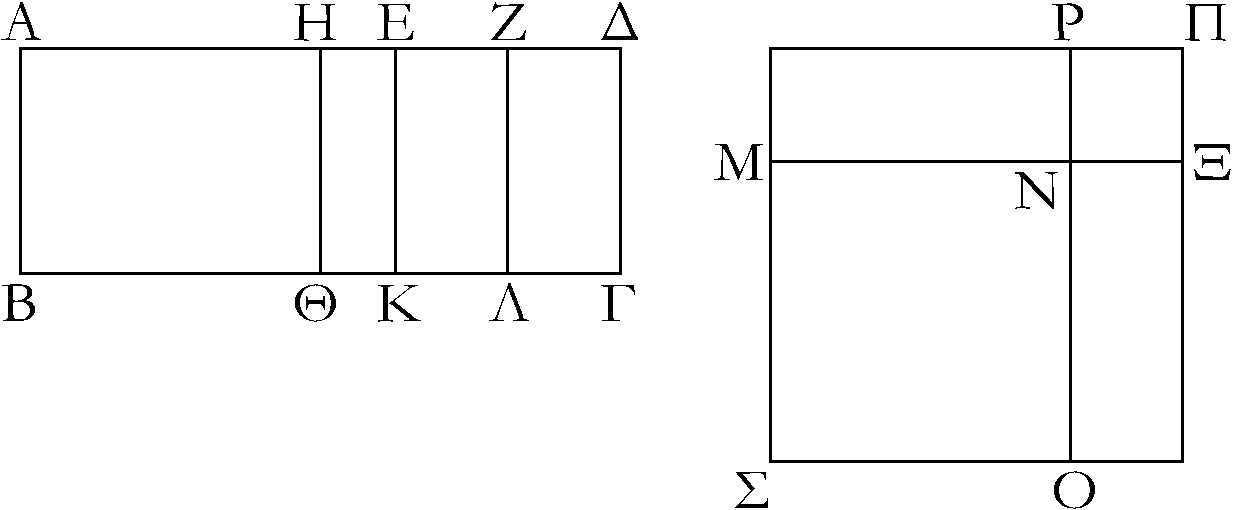
\includegraphics{Book10/fig054g.pdf}}

\gr{Θωρίον γὰρ τὸ ΑΓ περιεθέσθω ὑπὸ <ρητῆξ τῆξ ΑΒ καὶ τῆξ ἐκ δύο
ὀνομάτων πρώτηξ τῆξ ΑΔ; λέγω, <ότι ἡ τὸ ΑΓ θωρίον δυναμένη
>άλογόξ ἐστιν ἡ καλουμένη ἐκ δύο ὀνομάτων.}

\gr{Ἐπεὶ γὰρ ἐκ δύο ὀνομάτων ἐστὶ πρώτη ἡ ΑΔ, διῃρήσθω
εἰξ τὰ ὀνόματα κατὰ τὸ Ε, καὶ >έστω τὸ μεῖζον >όνομα τὸ
ΑΕ. φανερὸν δή, <ότι αἱ ΑΕ, ΕΔ <ρηταί εἰσι δυνάμει μόνον σύμμετροι,
καὶ ἡ ΑΕ τῆξ ΕΔ μεῖζον δύναται τῶ| ἀπὸ συμμέτρου ἑαυτῃ, καὶ
ἡ ΑΕ σύμμετρόξ ἐστι τῆ| ἐκκειμένῃ <ρητῆ| τῆ| ΑΒ μ\kern -.7pt  ήκει.
τετμ\kern -.7pt  ήσθω δὴ ἡ ΕΔ δίθα κατὰ τὸ Ζ σημεῖον. καὶ ἐπεὶ ἡ ΑΕ
τῆξ ΕΔ μεῖζον δύναται τῶ| ἀπὸ συμμέτρου ἑαυτῆ|, ἒαν >άρα
τῶ| τετάρτῳ μέρει τοῦ ἀπὸ τῆξ ἐλάσσονοξ, τουτέστι τῶ| ἀπὸ
τῆξ ΕΖ, >ίσον παρὰ τὴν μείζονα τὴν ΑΕ παραβληθῆ| ἐλλεῖπον
ε>ίδει τετραγώνῳ, εἰξ σύμμετρα α\kern -.5pt  ὐτὴν διαιρεῖ. παραβεβλήσθω ο~ὐν
παρὰ τὴν ΑΕ τῶ| ἀπὸ τῆξ ΕΖ >ίσον τὸ ὑπὸ ΑΗ, ΗΕ; σύμμετροξ
>άρα ἐστὶν ἡ ΑΗ τῆ| ΕΗ μ\kern -.3pt  ήκει. καὶ >ήθθωσαν ἀπὸ τῶν Η, Ε, Ζ
ὁποτέρᾳ τῶν ΑΒ, ΓΔ παράλληλοι αἱ ΗΘ, ΕΚ, ΖΛ; καὶ τῶ| μὲν
ΑΘ παραλληλογράμμῳ >ίσον τετράγωνον συνεστάτω τὸ ΣΝ, τῶ| δὲ
ΗΚ >ίσον τὸ ΝΠ, καὶ κείσθω <ώστε ἐπ> εὐθείαξ ε>ῖναι τὴν
ΜΝ τῆ| ΝΧ; ἐπ> εὐθείαξ >άρα ἐστὶ καὶ ἡ ΡΝ τῆ| ΝΟ. καὶ
συμπεπληρώσθω τὸ ΣΠ παραλληλόγραμμον; τετράγωνον >άρα ἐστὶ
τὸ ΣΠ. καὶ ἐπεὶ τὸ ὑπὸ τῶν ΑΗ, ΗΕ >ίσον ἐστὶ τῶ| ἀπὸ
τῆξ ΕΖ, >έστιν >άρα ὡξ ἡ ΑΗ πρὸξ ΕΖ, ο<ύτωξ ἡ ΖΕ πρὸξ ΕΗ; καὶ
ὡξ >άρα τὸ ΑΘ πρὸξ ΕΛ, τὸ ΕΛ πρὸξ ΚΗ; τῶν ΑΘ, ΗΚ >άρα μέσον
ἀνάλογόν ἐστι τὸ ΕΛ. ἀλλὰ τὸ μὲν ΑΘ >ίσον ἐστὶ τῶ| ΣΝ, τὸ δὲ
ΗΚ >ίσον τῶ| ΝΠ; τῶν ΣΝ, ΝΠ >άρα μέσον ἀνάλογόν ἐστι τὸ ΕΛ.
>έστι δὲ τῶν α\kern -.7pt  ὐτῶν τῶν ΣΝ, ΝΠ μέσον ἀνάλογον καὶ τὸ ΜΡ; >ίσον
>άρα ἐστὶ τὸ ΕΛ τῶ| ΜΡ; <ώστε καὶ τῶ| ΟΧ >ίσον ἐστίν. >έστι
δὲ καὶ τὰ ΑΘ, ΗΚ τοῖξ ΣΝ, ΝΠ >ίσα; <όλον >άρα τὸ ΑΓ >ίσον ἐστὶν
<όλῳ τῶ| ΣΠ, τουτέστι τῶ| ἀπὸ τῆξ ΜΧ τετραγώνῳ; τὸ ΑΓ
>άρα δύναται ἡ ΜΧ. λέγω, <ότι ἡ ΜΧ ἐκ δύο ὀνομάτων ἐστίν.}

\gr{Ἐπεὶ γὰρ σύμμετρόξ ἐστιν ἡ ΑΗ τῆ| ΗΕ, σύμμετρόξ ἐστι
καὶ ἡ ΑΕ ἑκατέρᾳ τῶν ΑΗ, ΗΕ. ὑπόκειται δὲ καὶ ἡ ΑΕ  τῆ| ΑΒ σύμμετροξ; καὶ αἱ
ΑΗ, ΗΕ >άρα τῆ| ΑΒ σύμμετροί εἰσιν. καί ἐστι <ρητὴ ἡ ΑΒ; <ρητὴ
>άρα ἐστὶ καὶ ἑκατέρα τῶν ΑΗ, ΗΕ; <ρητὸν >άρα ἐστὶν ἑκάτερον
τῶν ΑΘ, ΗΚ, καί ἐστι σύμμετρον τὸ ΑΘ τῶ| ΗΚ. ἀλλὰ τὸ μὲν ΑΘ
τῶ| ΣΝ >ίσον ἐστίν, τὸ δὲ ΗΚ τῶ| ΝΠ; καὶ
τὰ ΣΝ, ΝΠ >άρα,
τουτέστι τὰ ἀπὸ τῶν ΜΝ, ΝΧ, <ρητά ἐστι καὶ σύμμετρα. καὶ
ἐπεὶ ἀσύμμετρόξ ἐστιν ἡ ΑΕ τῆ| ΕΔ μ\kern -.7pt  ήκει, ἀλλ>
ἡ μὲν ΑΕ τῆ| ΑΗ ἐστι σύμμετροξ, ἡ δὲ ΔΕ τῆ| ΕΖ σύμμετροξ,
ἀσύμμετροξ >άρα καὶ ἡ ΑΗ τῆ| ΕΖ;
<ώστε καὶ τὸ ΑΘ τῶ| ΕΛ ἀσύμμετρόν ἐστιν. ἀλλὰ τὸ μὲν
ΑΘ τῶ| ΣΝ ἐστιν >ίσον, τὸ δὲ ΕΛ τῶ| ΜΡ; καὶ τὸ ΣΝ >άρα
τῶ| ΜΡ ἀσύμμετρόν ἐστιν. ἀλλ> ὡξ τὸ ΣΝ πρὸξ ΜΡ, ἡ ΟΝ
πρὸξ τὴν ΝΡ; ἀσύμμετροξ >άρα ἐστὶν ἡ ΟΝ τῆ| ΝΡ.
>ίση δὲ ἡ μὲν ΟΝ τῆ| ΜΝ, ἡ δὲ ΝΡ
τῆ| ΝΧ; ἀσύμμετροξ >άρα ἐστὶν ἡ ΜΝ τῆ| ΝΧ. καί
ἐστι τὸ ἀπὸ τῆξ ΜΝ σύμμετρον τῶ| ἀπὸ τῆξ ΝΧ, καὶ
<ρητὸν ἑκάτερον; αἱ ΜΝ, ΝΧ >άρα <ρηταί εἰσι
δυνάμει μόνον σύμμετροι.}

\gr{Ἡ ΜΧ >άρα ἐκ δύο ὀνομάτων ἐστὶ καὶ δύναται
τὸ ΑΓ; <όπερ >έδει δεῖχαι.}}

\ParallelRText{
\begin{center}
{\large Proposition 54}
\end{center}

If an area is contained by a rational (straight-line)
and a first binomial (straight-line) then  the  square-root  of the area is
the irrational (straight-line which is) called binomial.$^\dag$

% Removed epsf size command
\centerline{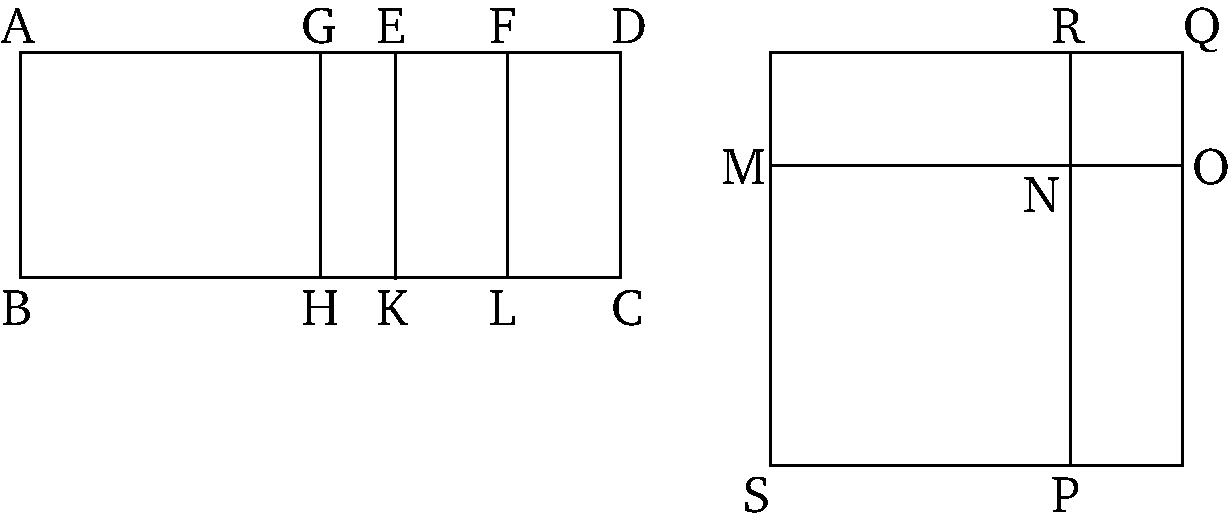
\includegraphics{Book10/fig054e.pdf}}

For let the area $AC$ be contained by the rational (straight-line) $AB$
and by the first binomial (straight-line) $AD$. I say that square-root of 
area $AC$ is the irrational (straight-line which is) called binomial.

For since $AD$ is a first binomial (straight-line), let it be divided
into its (component) terms at $E$, and let $AE$ be the greater term.
So, (it is) clear that $AE$ and $ED$ are rational (straight-lines which are)
commensurable in square only, and that the square on $AE$ is greater
than (the square on) $ED$ by the (square) on (some straight-line)
commensurable (in length) with ($AE$), and that $AE$ is commensurable 
(in length) with
the rational (straight-line) $AB$ (first) laid out [Def.~10.5]. So, let $ED$ be cut in half
at  point $F$. And since the square on $AE$ is greater than (the square on)
$ED$ by the (square) on (some straight-line) commensurable (in length) with ($AE$),
thus if a (rectangle) equal to the fourth part of the (square) on the lesser (term)---that is to say, the (square) on $EF$---falling short by a square figure,
is applied to the greater (term) $AE$, then it divides it into (terms which are)
commensurable (in length) [Prop~10.17]. 
Therefore, let the (rectangle contained) by $AG$ and $GE$, equal to
the (square) on $EF$, be applied to $AE$. $AG$ 
is thus commensurable in length with $EG$. And let $GH$, $EK$, and $FL$
be drawn from (points) $G$, $E$, and $F$ (respectively), parallel to
either of $AB$ or $CD$. And let the square $SN$, equal to the
parallelogram $AH$, be constructed, and (the square) $NQ$,
equal to (the parallelogram) $GK$ [Prop.~2.14].
And let $MN$ be laid down so as to be straight-on to $NO$. $RN$
is thus also straight-on to $NP$. And let the parallelogram $SQ$ 
be completed. $SQ$ is thus a square [Prop.~10.53~lem.].  And since the (rectangle
contained) by $AG$ and $GE$ is equal to the (square) on $EF$, thus as
$AG$ is to $EF$, so $FE$ (is) to $EG$ [Prop.~6.17]. And thus as $AH$ (is) to
$EL$, (so) $EL$ (is) to $KG$ [Prop.~6.1]. Thus,
$EL$ is the mean proportional to $AH$ and $GK$. But, $AH$ is equal to
$SN$, and $GK$ (is) equal to $NQ$. $EL$ is thus the mean proportional
to $SN$ and $NQ$. And $MR$ is also the mean proportional to the
same---(namely), $SN$ and $NQ$ [Prop.~10.53~lem.]. $EL$ is thus equal to $MR$.
Hence, it is also equal to $PO$ [Prop.~1.43]. And
$AH$ plus $GK$ is equal to $SN$ plus $NQ$. Thus, the whole of $AC$
is equal to the whole of $SQ$---that is to say, to the square on $MO$.
Thus, $MO$ (is) the square-root of (area) $AC$.  I say that $MO$ is a
binomial (straight-line).

For since $AG$ is commensurable (in length) with $GE$, $AE$ is also commensurable (in length)
with each of $AG$ and $GE$ [Prop.~10.15]. 
And $AE$ was also assumed (to be) commensurable (in length) with $AB$.  Thus,
$AG$ and $GE$ are also commensurable (in length) with $AB$
[Prop.~10.12]. And $AB$ is rational. $AG$
and $GE$ are thus each also  rational. Thus, $AH$ and $GK$ are each
rational (areas), and $AH$ is commensurable with $GK$ [Prop.~10.19]. But, $AH$ is equal to $SN$,
and $GK$ to $NQ$. $SN$ and $NQ$---that is to say, the (squares)
on $MN$ and $NO$ (respectively)---are thus also rational and commensurable. And since $AE$ is incommensurable in length with $ED$,
but $AE$ is commensurable (in length) with $AG$, and $DE$ (is) commensurable (in length)
with $EF$, $AG$ (is) thus also incommensurable (in length) with $EF$
[Prop.~10.13]. Hence, $AH$ is also incommensurable with $EL$ [Props.~6.1, 10.11]. But, $AH$ is equal to $SN$, and $EL$
to $MR$. Thus, $SN$ is also incommensurable with $MR$. But, as
$SN$ (is) to $MR$, (so) $PN$ (is) to $NR$ [Prop.~6.1].  $PN$ is thus incommensurable (in length) with $NR$ [Prop.~10.11]. And $PN$ (is) equal to $MN$, and $NR$ to
$NO$. Thus, $MN$ is incommensurable (in length) with $NO$. And the (square)
on $MN$ is commensurable with the (square) on $NO$, and each (is)
rational.  $MN$ and $NO$ are thus rational (straight-lines which are)
commensurable in square only.

Thus, $MO$ is (both) a binomial (straight-line) [Prop. 10.36], and the square-root of $AC$.
(Which is) the very thing it was required to show.}
\end{Parallel}
{\footnotesize\noindent $^\dag$ If the rational straight-line has unit length then this proposition states that the square-root of 
a first binomial straight-line is a binomial straight-line: {i.e.}, 
a first binomial straight-line has a length $k+k\,\sqrt{1-k'^{\,2}}$ whose
square-root can be written $\rho\,(1+\sqrt{k''})$, where $\rho=\sqrt{k\,(1+k')/2}$ and $k''=(1-k')/(1+k')$. This is the length of a binomial straight-line (see Prop.~10.36), since $\rho$ is rational.}

%%%%
%10.55
%%%%
\pdfbookmark[1]{Proposition 10.55}{pdf10.55}
\begin{Parallel}{}{}
\ParallelLText{
\begin{center}
{\large \ggn{55}.}
\end{center}\vspace*{-7pt}

\gr{Ἐὰν θωρίον περιέθηται ὑπὸ <ρητῆξ καὶ τῆξ ἐκ δύο ὁνομάτων
δευτέραξ, ἡ τὸ θωρίον δυναμένη >άλογόξ ἐστιν ἡ καλουμένη
ἐκ δύο μέσων πρώτη.}

% Removed epsf size command
\centerline{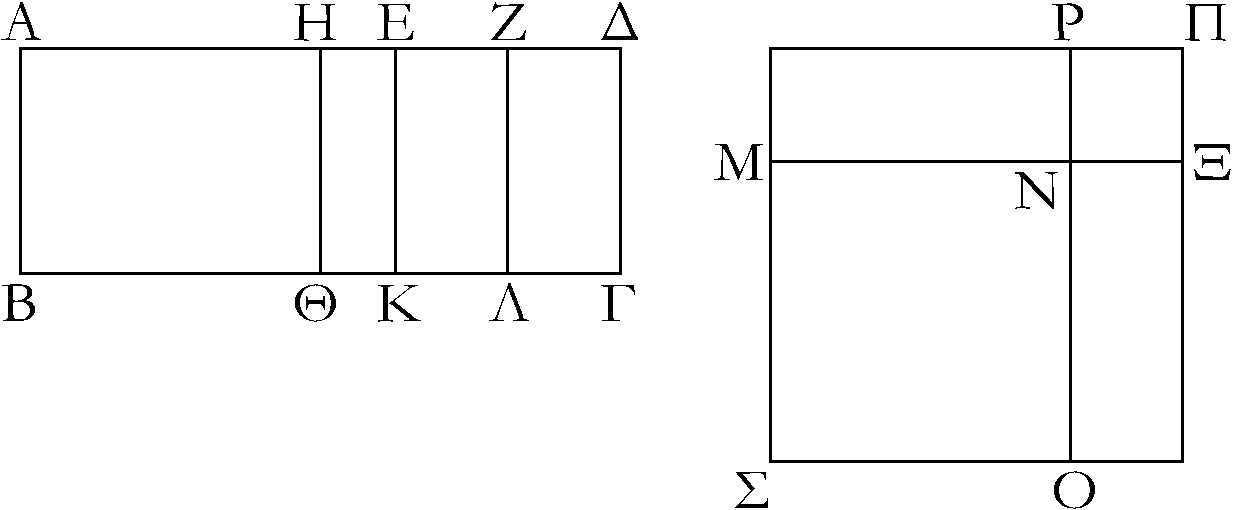
\includegraphics{Book10/fig054g.pdf}}

\gr{Περιεθέσθω γὰρ θωρίον τὸ ΑΒΓΔ ὑπὸ <ρητῆξ τῆξ ΑΒ  καὶ τῆξ
ἐκ δύο ὀνομάτων δυετέραξ τῆξ ΑΔ; λέγω, <ότι ἡ τὸ ΑΓ θωρίον
δυναμένη ἐκ δύο μέσων πρώτη ἐστίν.}

\gr{Ἐπεὶ γὰρ ἐκ δύο ὀνομάτων δευτέρα ἐστὶν ἡ ΑΔ, διῃρήσθω εἰξ
τὰ ὀνόματα κατὰ τὸ Ε, <ώστε τὸ μεῖζον >όνομα ε>ῖναι τὸ ΑΕ;
αἱ ΑΕ, ΕΔ >άρα <ρηταί εἰσι δυνάμει μόνον σύμμετροι, καὶ ἡ ΑΕ
τῆξ ΕΔ μεῖζον δύναται τῶ| ἀπὸ συμμέτρου ἑαυτῆ|, καὶ τὸ
>έλαττον >όνομα ἡ ΕΔ σύμμετρόν ἐστι τῆ| ΑΒ μ\kern -.7pt  ήκει. τετμ\kern -.7pt  ήσθω
ἡ ΕΔ δίθα κατὰ τὸ Ζ, καὶ τῶ| ἀπὸ τῆξ ΕΖ >ίσον παρὰ τὴν ΑΕ
παραβεβλήσθω ἐλλεῖπον ε>ίδει τετραγώνῳ τὸ ὑπὸ τῶν
ΑΗΕ; σύμμετροξ >άρα ἡ ΑΗ τῆ| ΗΕ μ\kern -.5pt  ήκει. καὶ  διὰ τῶν Η, Ε, Ζ
παράλληλοι >ήθθωσαν ταῖξ ΑΒ, ΓΔ αἱ ΗΘ, ΕΚ, ΖΛ, καὶ τῶ| μὲν
ΑΘ παραλληλογράμμῳ >ίσον τετράγωνον συνεστάτω τὸ ΣΝ, τῶ| δὲ ΗΚ
>ίσον τετράγωνον 
τὸ ΝΠ, καὶ κείσθω <ώστε ἐπ> εὐθείαξ ε>ῖναι τὴν ΜΝ τῆ| ΝΧ; ἐπ>
εὐθείαξ >άρα [ἐστὶ] καὶ ἡ ΡΝ τῆ ΝΟ. καὶ συμπεπληρώσθω
τὸ ΣΠ τετράγωνον;  φανερὸν δὴ ἐκ τοῦ προδεδειγμένου, <ότι τὸ ΜΡ
μέσον ἀνάλογόν ἐστι τῶν ΣΝ, ΝΠ, καὶ >ίσον τῶ| ΕΛ, καὶ
<ότι τὸ ΑΓ θωρίον δύναται ἡ ΜΧ. δεικτέον δή, <ότι ἡ ΜΧ ἐκ
δύο μέσων ἐστὶ πρώτη.}

\gr{Ἐπεὶ ἀσύμμετρόξ ἐστιν ἡ ΑΕ τῆ| ΕΔ
μ\kern -.7pt  ήκει, σύμμετροξ δὲ ἡ ΕΔ τῆ| ΑΒ, ἀσύμμετροξ >άρα ἡ ΑΕ τῆ|
ΑΒ. καὶ ἐπεὶ σύμμετρόξ ἐστιν ἡ ΑΗ τῆ| ΕΗ, σύμμετρόξ ἐστι
καὶ ἡ ΑΕ ἑκατέρᾳ τῶν ΑΗ, ΗΕ. ἀλλὰ ἡ ΑΕ ἀσύμμετροξ τῆ|
ΑΒ μ\kern -.7pt  ήκει; καὶ αἱ ΑΗ, ΗΕ >άρα ἀσύμμετροί εἰσι τῆ| ΑΒ. αἱ ΒΑ,
ΑΗ, ΗΕ >άρα <ρηταί εἰσι δυνάμει μόνον σύμμετροι; <ώστε μέσον
ἐστὶν ἑκάτερον τῶν ΑΘ, ΗΚ. <ώστε καὶ ἑκάτερον τῶν ΣΝ, ΝΠ
μέσον ἐστίν. καὶ αἱ ΜΝ, ΝΧ >άρα μέσαι εἰσίν. καὶ ἐπεὶ
σύμμετροξ ἡ ΑΗ τῆ| ΗΕ μ\kern -.5pt  ήκει, σύμμετρόν ἐστι καὶ τὸ ΑΘ τῶ|
ΗΚ, τουτέστι τὸ ΣΝ τῶ| ΝΠ, τουτέστι τὸ ἀπὸ τῆξ ΜΝ τῶ| ἀπὸ
τῆξ ΝΧ [<ώστε δυνάμει εἰσὶ σύμμετροι αἱ ΜΝ, ΝΧ]. καὶ
ἐπεὶ ἀσύμμετρόξ ἐστιν ἡ ΑΕ τῆ| ΕΔ μ\kern -.3pt  ήκει, ἀλλ> ἡ μὲν ΑΕ
σύμμετρόξ ἐστι τῆ| ΑΗ, ἡ δὲ ΕΔ τῆ| ΕΖ σύμμετροξ, ἀσύμμετροξ >άρα ἡ ΑΗ τῆ| ΕΖ; <ώστε καὶ τὸ ΑΘ τῶ| ΕΛ ἀσύμμετρόν ἐστιν,
τουτέστι τὸ ΣΝ τῶ| ΜΡ, τουτέστιν ὁ ΟΝ τῆ| ΝΡ, τουτέστιν
ἡ ΜΝ τῆ| ΝΧ ἀσύμμετρόξ ἐστι μ\kern -.7pt  ήκει.  ἐδείθθησαν δὲ αἱ ΜΝ,
ΝΧ καὶ μέσαι ο>ῦσαι καὶ δυνάμει σύμμετροι; αἱ ΜΝ, ΝΧ >άρα
μέσαι εἰσὶ δυνάμει μόνον σύμμετροι. λέγω δή, <ότι καὶ <ρητὸν
περιέθουσιν. ἐπεὶ γὰρ ἡ ΔΕ ὑπόκειται ἑκατέρᾳ τῶν ΑΒ, ΕΖ σύμμετροξ, σύμμετροξ >άρα καὶ ἡ ΕΖ τῆ| ΕΚ. καὶ <ρητὴ ἑκατέρα
α\kern -.7pt  ὐτῶν; <ρητὸν >άρα τὸ ΕΛ, τουτέστι τὸ ΜΡ; τὸ δὲ ΜΡ ἐστι
τὸ ὑπὸ τῶν ΜΝΧ. ἒαν δὲ δύο μέσαι δυνάμει μόνον σύμμετροι
συντεθῶσι <ρητὸν περιέθουσαι, ἡ <όλη >άλογόξ ἐστιν, καλεῖται δὲ ἐκ δύο μέσων πρώτη.}

\gr{Ἡ >άρα ΜΧ ἐκ δύο μέσων ἐστὶ πρώτη; <όπερ >έδει δεῖχαι.}}

\ParallelRText{
\begin{center}
{\large Proposition 55}
\end{center}

If an area is contained by a rational (straight-line)
and a second binomial (straight-line) then the square-root of the area
is the irrational (straight-line which is) called first bimedial.$^\dag$

% Removed epsf size command
\centerline{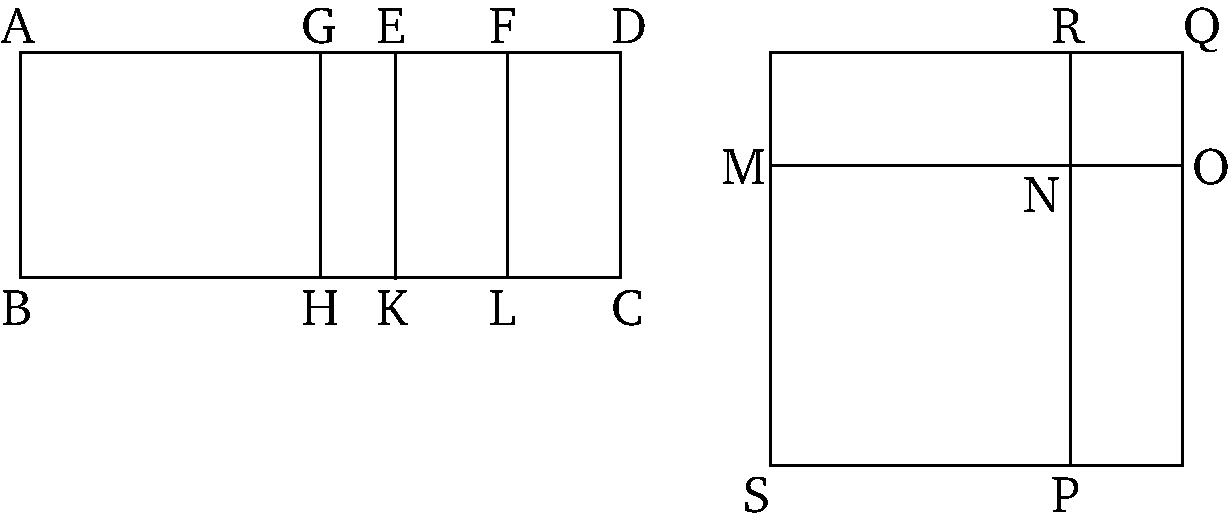
\includegraphics{Book10/fig054e.pdf}}

For let the area $ABCD$ be contained by the rational (straight-line) $AB$
and by the second binomial (straight-line)  $AD$. I say that the square-root
of  area $AC$ is a first bimedial (straight-line).\

For since $AD$ is a second binomial (straight-line), let it be divided
into its (component) terms at $E$, such that $AE$ is the greater term. Thus,
$AE$ and $ED$ are rational (straight-lines which are) commensurable
in square only, and the square on $AE$ is greater than (the square on)
$ED$ by the (square) on (some straight-line) commensurable (in length) with ($AE$),
and the lesser term $ED$ is commensurable in length with $AB$ [Def.~10.6].  Let $ED$ be cut in half at $F$.
And let the (rectangle contained) by $AGE$, equal to the (square) on $EF$,
 be applied to $AE$, falling short by a square figure. $AG$
(is) thus commensurable in length with $GE$ [Prop.~10.17]. And let $GH$, $EK$, and
$FL$ be drawn through (points) $G$, $E$, and $F$ (respectively), parallel
to $AB$ and $CD$. And let the square $SN$, equal to the parallelogram
$AH$, be constructed, and the square $NQ$, equal to
$GK$.  And let $MN$ be laid down so as to be straight-on to $NO$. Thus,
$RN$ [is] also straight-on to $NP$. And let the square $SQ$ be
completed. So, (it is) clear from what has been previously
demonstrated [Prop.~10.53~lem.] that
$MR$ is the mean proportional to $SN$ and $NQ$, and (is) equal to
$EL$, and that $MO$ is the square-root of the area $AC$. So, we
must show that $MO$ is a first bimedial (straight-line).

Since $AE$
is incommensurable in length with $ED$, and $ED$ (is) commensurable 
 (in length) with $AB$, $AE$ (is) thus incommensurable (in length) with $AB$ [Prop.~10.13]. And since $AG$
is commensurable (in length) with $EG$, $AE$ is also commensurable
(in length) with each of $AG$ and $GE$ [Prop.~10.15]. 
But, $AE$ is incommensurable in length with $AB$.  Thus, $AG$ and $GE$
are also (both) 
incommensurable (in length) with $AB$ [Prop.~10.13]. 
Thus, $BA$, $AG$,  and ($BA$, and) $GE$ are (pairs of) rational (straight-lines which are)
commensurable in square only. And, hence, each of $AH$ and $GK$ is a medial
(area) [Prop.~10.21]. Hence, each of $SN$ and $NQ$
is also a medial (area). Thus, $MN$ and $NO$ are medial (straight-lines). 
And since $AG$ (is) commensurable in length with $GE$, $AH$
is also commensurable with $GK$---that is to say, $SN$ with $NQ$---that is to say, the (square)
on $MN$  with the (square) on $NO$ [hence, $MN$ and $NO$
are commensurable in square] [Props.~6.1, 10.11]. And since $AE$ is incommensurable
in length with $ED$, but $AE$ is commensurable (in length) with $AG$,
and $ED$ commensurable (in length) with $EF$, $AG$ (is) thus
incommensurable (in length) with $EF$ [Prop.~10.13]. Hence, $AH$ is also incommensurable with $EL$---that is to say, $SN$ with $MR$---that is to
say, $PN$ with $NR$---that is to say, $MN$ is incommensurable
in length with $NO$  [Props.~6.1, 10.11]. But $MN$ and $NO$ have also
been shown to be medial (straight-lines) which are commensurable in square. 
Thus, $MN$ and $NO$ are medial (straight-lines which are) commensurable
in square only.
So,
I say that they also contain a rational (area). For since $DE$ was assumed
(to be) commensurable (in length) with each of $AB$ and $EF$, $EF$
(is) thus also commensurable with $EK$ [Prop.~10.12]. And they (are) each rational.
Thus, $EL$---that is to say, $MR$---(is) rational [Prop.~10.19]. And $MR$ is the (rectangle contained) by $MNO$. And if two medial (straight-lines), commensurable
in square only, which contain a rational (area), are added together, then the
whole is (that) irrational (straight-line which is)
called first bimedial [Prop.~10.37].

Thus, $MO$ is a first bimedial (straight-line). (Which is) the very thing it
was required to show.}
\end{Parallel}
{\footnotesize\noindent$^\dag$ If the rational straight-line has unit length then this proposition states that the square-root of 
a second binomial straight-line is a first bimedial straight-line: {i.e.}, 
a second binomial straight-line has a length $k/\sqrt{1-k'^{\,2}}+k$ whose
square-root can be written $\rho\,(k''^{1/4}+k''^{3/4})$, where $\rho=\sqrt{(k/2)\,(1+k')/(1-k')}$ and $k''=(1-k')/(1+k')$. This is the length of a first bimedial straight-line (see Prop.~10.37), since $\rho$ is rational.}

%%%%
%10.56
%%%%
\pdfbookmark[1]{Proposition 10.56}{pdf10.56}
\begin{Parallel}{}{}
\ParallelLText{
\begin{center}
{\large \ggn{56}.}
\end{center}\vspace*{-7pt}

\gr{Ἐὰν θωρίον περιέθηται ὑπὸ <ρητῆξ καὶ τῆξ ἐκ
δύο ὀνομάτων τρίτηξ, ἡ τὸ θωρίον δυναμένη >άλογόξ ἐστιν
ἡ καλουμένη ἐκ δύο μέσων δευτέρα.}

\gr{Θωρίον γὰρ τὸ ΑΒΓΔ περιεθέσθω ὑπὸ <ρητῆξ τῆξ ΑΒ καὶ τῆξ
ἐκ δύο ὀνομάτων τρίτηξ τῆξ ΑΔ διῃρημένηξ εἰξ τὰ ὀνόματα
κατὰ τὸ Ε, <ῶν μεῖζόν ἐστι τὸ ΑΕ; λέγω,  <ότι ἡ τὸ ΑΓ
θωρίον δυναμένη >άλογόξ ἐστιν ἡ καλουμένη ἐκ δύο μέσων
δευτέρα.}

% Removed epsf size command
\centerline{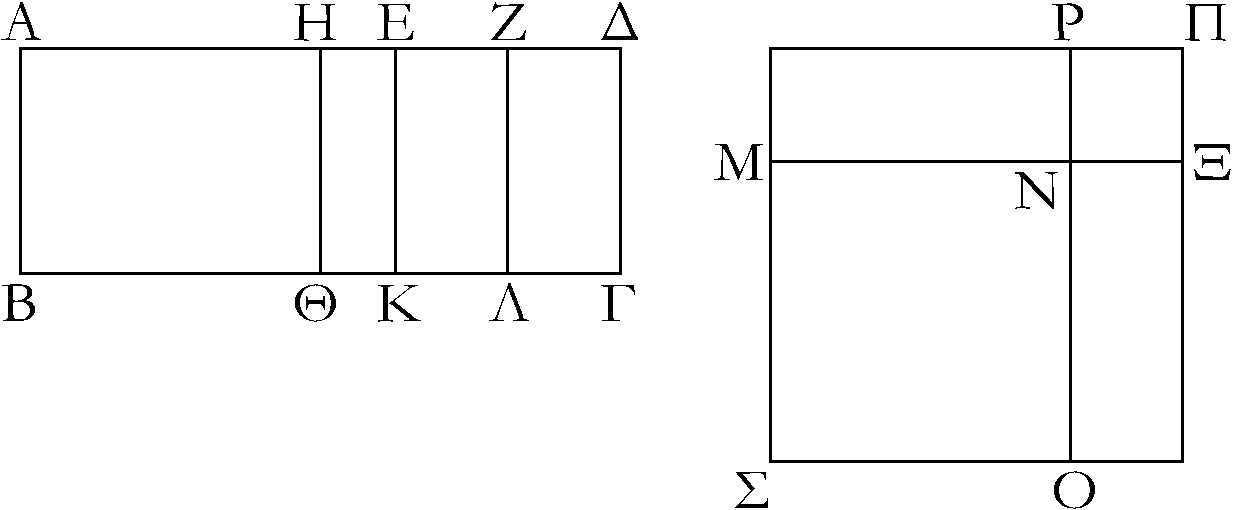
\includegraphics{Book10/fig054g.pdf}}

\gr{Κατεσκευάσθω γὰρ τὰ α\kern -.7pt  ὐτὰ τοῖξ πρότερον. καὶ ἐπεὶ ἐκ δύο
ὀνομάτων ἐστὶ τρίτη ἡ ΑΔ, αἱ ΑΕ, ΕΔ >άρα <ρηταί εἰσι
δυνάμει μόνον σύμμετροι, καὶ ἡ ΑΕ τῆξ ΕΔ μεῖζον δύναται
τῶ| ἀπὸ συμμέτρου ἑαυτῆ|, καὶ οὐδετέρα τῶν ΑΕ, ΕΔ
σύμμετρόξ [ἐστι] τῆ| ΑΒ μ\kern -.7pt  ήκει. ὁμοίωξ δὴ τοῖξ προδεδειγμένοιξ
δείχομεν, <ότι ἡ ΜΧ ἐστιν ἡ τὸ ΑΓ θωρίον δυναμένη, καὶ αἱ ΜΝ,
ΝΧ μέσαι εἰσὶ δυνάμει μόνον σύμμετροι; <ώστε ἡ ΜΧ ἐκ δύο
μέσων ἐστίν. δεικτέον δή, <ότι καὶ δευτέρα.}

\gr{\kern -.7pt {[}Ka`i] >epe`i >as'ummetr'oc >estin <h DE t~h| AB m\kern -.7pt 'hkei, tout'esti
t~h| EK, s'ummetroc d`e <h DE t~h| EZ, >as'ummetroc >'ara >est`in
<h EZ t~h| EK m\kern -.7pt 'hkei. ka'i e>isi <rhta'i; a<i ZE, EK >'ara <rhta'i
e>isi dun'amei m'onon s'ummetroi. m'eson >'ara [>est`i] t`o EL,
tout'esti t`o MR; ka`i peri'eqetai <up`o t~wn MNX; m'eson >'ara >est`i
t`o <up`o t~wn MNX.}

\gr{Ἡ ΜΧ >άρα ἐκ δύο μέσων ἐστὶ δευτέρα; <όπερ >έδει δεῖχαι.}}

\ParallelRText{
\begin{center}
{\large Proposition 56}
\end{center}

If an area is contained by a rational (straight-line)
and a third binomial (straight-line) then the square-root of the area is
the irrational (straight-line which is) called second bimedial.$^\dag$

For let the area $ABCD$ be contained by the rational (straight-line)
$AB$ and by the third binomial (straight-line) $AD$, which has been divided into
its (component) terms at $E$, of which $AE$ is the greater.  I say that
the square-root of area $AC$ is the irrational (straight-line which is)
called second bimedial.

% Removed epsf size command
\centerline{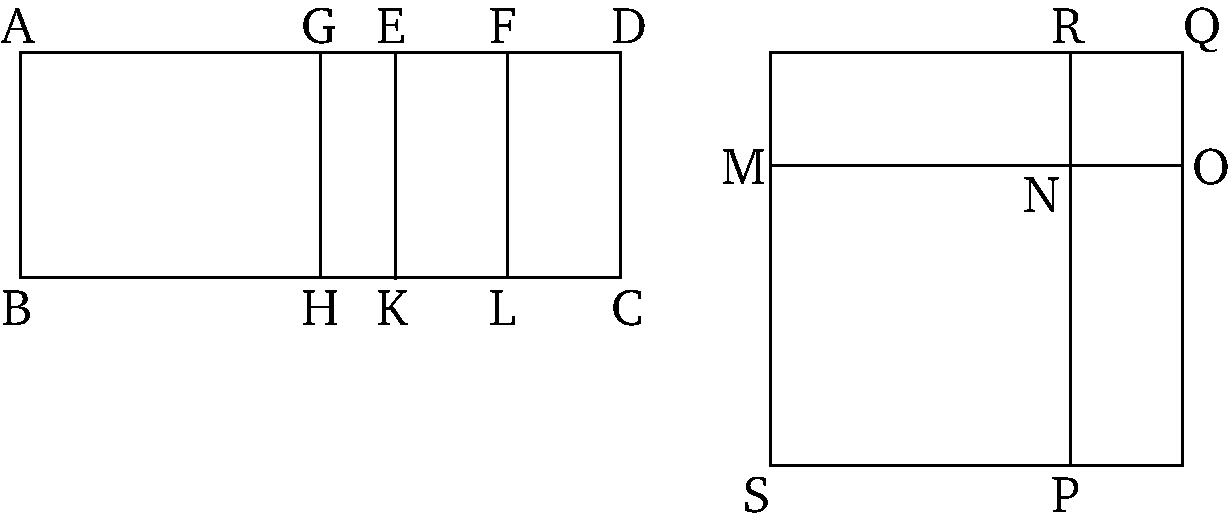
\includegraphics{Book10/fig054e.pdf}}

For let the same construction be made as  previously. And since
$AD$ is a third binomial (straight-line), $AE$ and $ED$
are thus rational (straight-lines which are) commensurable in square only,
and the square on $AE$ is greater than (the square on) $ED$
by the (square) on (some straight-line) commensurable (in length) with
($AE$), and neither of $AE$ and $ED$ [is] commensurable in length
with $AB$ [Def.~10.7]. So, similarly
to that which has been previously demonstrated, we can show that
$MO$ is the square-root of  area $AC$, and $MN$ and $NO$
are medial (straight-lines which are) commensurable in square only.
Hence, $MO$ is bimedial. So, we must show that (it is)
also second (bimedial).

\mbox{[}And] since $DE$ is incommensurable in length with $AB$---that is to say,
with $EK$---and $DE$ (is) commensurable (in length) with $EF$,
$EF$ is thus incommensurable in length with $EK$ [Prop.~10.13]. And they are (both)
rational (straight-lines). Thus, $FE$ and $EK$ are rational (straight-lines which are) commensurable in square only. $EL$---that is to say, $MR$---[is] thus medial [Prop.~10.21]. And it
is contained by $MNO$.  Thus, the (rectangle contained) by $MNO$
is medial.

Thus, $MO$ is a second bimedial (straight-line) [Prop. 10.38]. (Which is) the very thing it was required to show.}
\end{Parallel}
{\footnotesize\noindent $^\dag$ If the rational straight-line has unit length then this proposition states that the square-root of 
a third binomial straight-line is a second bimedial straight-line: {i.e.}, 
a third binomial straight-line has a length $k^{1/2}\,(1+\sqrt{1-k'^{\,2}})$ whose
square-root can be written $\rho\,(k^{1/4}+k''^{1/2}/k^{1/4})$, where $\rho=\sqrt{(1+k')/2}$ and $k''=k\,(1-k')/(1+k')$. This is the length of a second bimedial straight-line (see Prop.~10.38), since $\rho$ is rational.}

%%%%
%10.57
%%%%
\pdfbookmark[1]{Proposition 10.57}{pdf10.57}
\begin{Parallel}{}{}
\ParallelLText{
\begin{center}
{\large \ggn{57}.}
\end{center}\vspace*{-7pt}

\gr{Ἐὰν θωρίον περιέθηται ὑπὸ <ρητῆξ καὶ τῆξ ἐκ δύο ὀνομάτων
τετάρτηξ, ἡ τὸ θωρίον δυναμένη >άλογόξ ἐστιν ἡ καλουμένη 
μείζων.}

% Removed epsf size command
\centerline{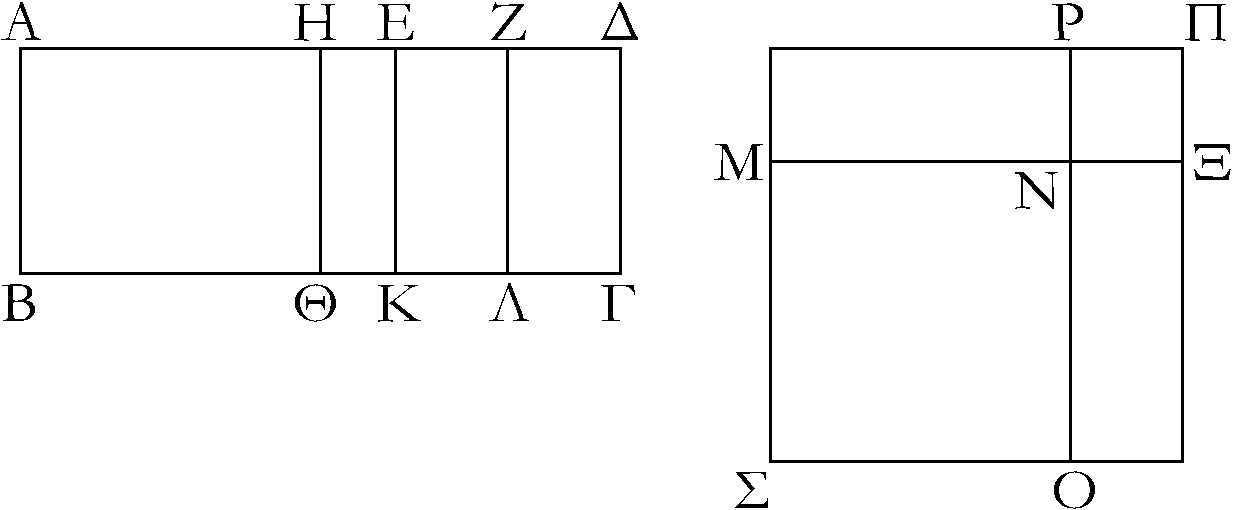
\includegraphics{Book10/fig054g.pdf}}

\gr{Θωρίον γὰρ τὸ ΑΓ περιεθέσθω ὑπὸ <ρητῆξ τῆξ ΑΒ καὶ τῆξ
ἐκ δύο ὀνομάτων τετάρτηξ τῆξ ΑΔ διῃρημένηξ εἰξ τὰ
ὀνόματα κατὰ τὸ Ε, <ῶν μεῖζον >έστω τὸ ΑΕ; λέγω, <ότι
ἡ τὸ ΑΓ θωρίον δυναμένη >άλογόξ ἐστιν ἡ καλουμένη
μείζων.}

\gr{Ἐπεὶ γὰρ ἡ ΑΔ ἐκ δύο ὀνομάτων ἐστὶ τετάρτη, αἱ ΑΕ, ΕΔ
>άρα <ρηταί εἰσι δυνάμει μόνον σύμμετροι, καὶ ἡ ΑΕ τῆξ
ΕΔ μεῖζον δύναται τῶ| ἀπὸ ἀσυμμέτρου ἑαυτῆ|, καὶ ἡ ΑΕ
τῆ| ΑΒ σύμμετρόξ [ἐστι] μ\kern -.7pt  ήκει. τετμ\kern -.7pt  ήσθω ἡ ΔΕ δίθα κατὰ
τὸ Ζ, καὶ τῶ| ἀπὸ τῆξ ΕΖ >ίσον παρὰ τὴν ΑΕ παραβεβλήσθω
παραλληλόγραμμον τὸ ὑπὸ ΑΗ, ΗΕ; ἀσύμμετροξ >άρα ἐστὶν
ἡ ΑΗ τῆ| ΗΕ μ\kern -.5pt  ήκει. >ήθθωσαν παράλληλοι τῆ| ΑΒ αἱ ΗΘ, ΕΚ, 
ΖΛ, καὶ τὰ λοιπὰ τὰ α\kern -.3pt  ὐτὰ τοῖξ πρὸ τούτου γεγονέτω;
φανερὸν δή, <ότι ἡ τὸ ΑΓ θωρίον δυναμένη ἐστὶν ἡ
ΜΧ. δεικτέον δή, <ότι ἡ ΜΧ >άλογόξ ἐστιν ἡ καλουμένη
μείζων.}

\gr{Ἐπεὶ ἀσύμμετρόξ ἐστιν ἡ ΑΗ τῆ| ΕΗ μ\kern -.7pt  ήκει, ἀσύμμετρόν
ἐστι καὶ τὸ ΑΘ τῶ| ΗΚ, τουτέστι τὸ ΣΝ τῶ| ΝΠ; αἱ ΜΝ, ΝΧ >άρα δυνάμει εἰσὶν ἀσύμμετροι. καὶ ἐπεὶ σύμμετρόξ ἐστιν ἡ ΑΕ
τῆ| ΑΒ μ\kern -.7pt  ήκει, <ρητόν ἐστι τὸ ΑΚ; καί ἐστιν >ίσον τοῖξ
ἀπὸ τῶν ΜΝ, ΝΧ; <ρητὸν >άρα [ἐστὶ] καὶ τὸ συγκείμενον
ἐκ τῶν ἀπὸ τῶν ΜΝ, ΝΧ. καὶ ἐπεὶ ἀσύμμετρόξ
[ἐστιν] ἡ ΔΕ τῆ| ΑΒ μ\kern -.5pt  ήκει, τουτέστι  τῆ| ΕΚ, ἀλλὰ
ἡ ΔΕ σύμμετρόξ ἐστι τῆ| ΕΖ, ἀσύμμετροξ >άρα ἡ ΕΖ
τῆ| ΕΚ μ\kern -.3pt  ήκει. αἱ ΕΚ, ΕΖ >άρα <ρηταί εἰσι δυνάμει μόνον σύμμετροι;
μέσον >άρα τὸ ΛΕ, τουτέστι τὸ ΜΡ. καὶ περιέθεται ὑπὸ τῶν
ΜΝ, ΝΧ; μέσον >άρα ἐστὶ τὸ ὑπὸ τῶν ΜΝ, ΝΧ. καὶ <ρητὸν
τὸ [συγκείμενον] ἐκ τῶν ἀπὸ τῶν ΜΝ, ΝΧ, καί εἰσιν ἀσύμμετροι
αἱ ΜΝ, ΝΧ δυνάμει. ἒαν δὲ δύο εὐθεῖαι δυνάμει ἀσύμμετροι
συντεθῶσι ποιοῦσαι τὸ μὲν συγκείμενον ἐκ τῶν ἀπ> α\kern -.7pt  ὐτῶν
τετραγώνων <ρητόν, τὸ δ> ὑπ> α\kern -.7pt  ὐτῶν μέσον, ἡ <όλη >άλογόξ
ἐστιν, καλεῖται δὲ μείζων.}

\gr{Ἡ ΜΧ >άρα >άλογόξ ἐστιν ἡ καλουμένη μείζων, καὶ δύναται
τὸ ΑΓ θωρίον; <όπερ >έδει δεῖχαι.}}

\ParallelRText{
\begin{center}
{\large Proposition 57}
\end{center}

If an area is contained by a rational (straight-line)
and a fourth binomial (straight-line) then the square-root of the area
is the irrational (straight-line which is) called major.$^\dag$

% Removed epsf size command
\centerline{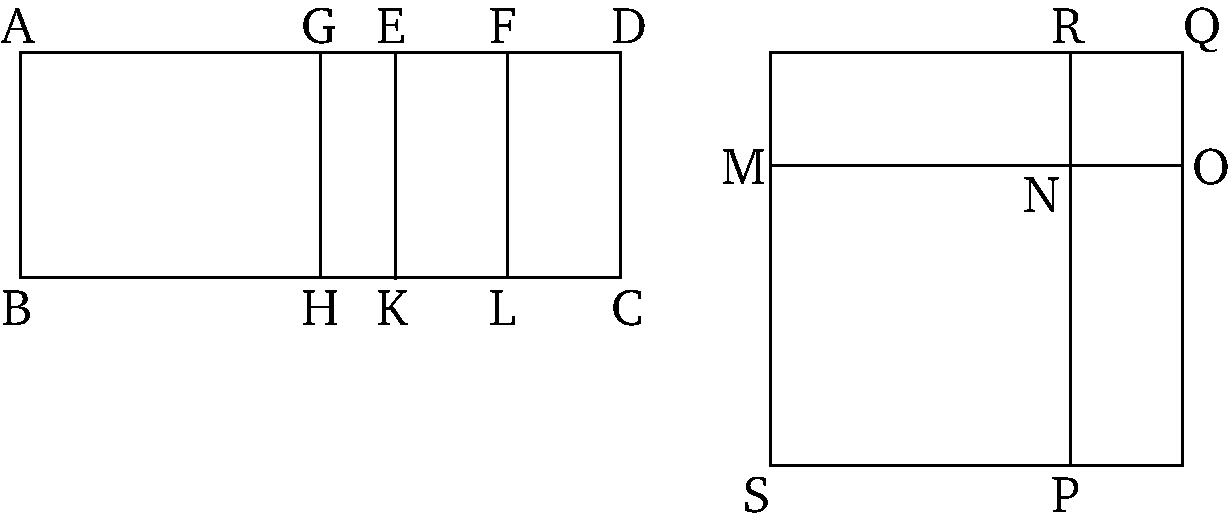
\includegraphics{Book10/fig054e.pdf}}

For let the area $AC$ be contained by the rational (straight-line) $AB$
and the fourth binomial (straight-line) $AD$, which has been divided into
its (component) terms at $E$, of which let $AE$ be the greater. I say that
the square-root of $AC$ is the irrational (straight-line which is) called major.

For since $AD$ is a fourth binomial (straight-line), $AE$ and $ED$
are thus rational (straight-lines which are) commensurable in square only,
and the square on $AE$ is greater than (the square on) $ED$ by the
(square) on (some straight-line) incommensurable (in length) with ($AE$),
and $AE$ [is] commensurable in length with $AB$ [Def.~10.8]. Let $DE$ be cut in half at $F$,
and let the parallelogram (contained by) $AG$ and $GE$, equal to the
(square) on $EF$, (and falling short by a square figure) be applied to
$AE$. $AG$ is thus incommensurable in length with $GE$ [Prop.~10.18]. Let $GH$, $EK$, and $FL$
be drawn parallel to $AB$, and let the rest (of the construction) be made the same as the (proposition) before this. So, it is clear that
$MO$ is the square-root of  area $AC$. So, we must show that $MO$
is the irrational (straight-line which is) called major.

Since $AG$ is incommensurable in length with $EG$, $AH$
is also incommensurable with $GK$---that is to say, $SN$
 with $NQ$ [Props.~6.1, 10.11].  Thus, $MN$ and $NO$
 are incommensurable in square. And since $AE$ is
 commensurable in length with $AB$, $AK$ is rational [Prop.~10.19].  And it is equal to the (sum of the squares) on $MN$ and $NO$.  Thus, the sum of the (squares) on 
 $MN$ and $NO$ [is] also rational. And since $DE$ [is]  incommensurable
 in length with $AB$ [Prop.~10.13]---that is to say, with $EK$---but $DE$ is commensurable (in length) with $EF$, $EF$ (is) thus incommensurable
 in length with $EK$ [Prop.~10.13].
 Thus, $EK$ and $EF$ are rational (straight-lines which are) commensurable
 in square only. $LE$---that is to say, $MR$---(is) thus medial
 [Prop.~10.21]. And it is contained by $MN$ and $NO$. The (rectangle contained) by $MN$ and $NO$ is thus medial. And
 the [sum] of the (squares) on $MN$ and $NO$ (is) rational, and
 $MN$ and $NO$ are incommensurable in square. And if two
 straight-lines (which are) incommensurable in square, making the
 sum of the squares on them rational, and the (rectangle contained) by them
 medial, are added together, then the whole is the irrational (straight-line which is) called major [Prop.~10.39].
 
 Thus, $MO$ is the irrational (straight-line which is) called major.
 And (it is) the square-root of area $AC$. (Which is) the very thing it
 was required to show.}
\end{Parallel}
 {\footnotesize\noindent$^\dag$ If the rational straight-line has unit length then this proposition states that the square-root of 
a fourth binomial straight-line is a major straight-line: {i.e.}, 
a fourth binomial straight-line has a length $k\,(1+1/\sqrt{1+k'})$ whose
square-root can be written $\rho\,\sqrt{[1+k''/(1+k''^{\,2})^{1/2}]/2}+\rho\,\sqrt{[1-k''/(1+k''^{\,2})^{1/2}]/2}$, where $\rho=\sqrt{k}$ and $k''^{\,2}=k'$. This is the length of a major straight-line (see Prop.~10.39), since $\rho$ is rational.}

%%%%
%10.58
%%%%
\pdfbookmark[1]{Proposition 10.58}{pdf10.58}
\begin{Parallel}{}{}
\ParallelLText{
\begin{center}
{\large \ggn{58}.}
\end{center}\vspace*{-7pt}

\gr{Ἐὰν θωρίον περιέθηται ὑπὸ <ρητῆξ καὶ τῆξ ἐκ δύο ὀνομάτων
πέμπτηξ, ἡ τὸ θωρίον δυναμένη >άλογόξ ἐστιν ἡ καλουμένη
<ρητὸν καὶ μέσον δυναμένη.}

\gr{Θωρίον γὰρ τὸ ΑΓ περιεθέσθω ὑπὸ <ρητῆξ τῆξ ΑΒ καὶ τῆξ ἐκ
δύο ὀνομάτων πέμπτηξ τῆξ ΑΔ διῃρημένηξ εἰξ τὰ ὀνόματα
κατὰ τὸ Ε, <ώστε τὸ μεῖζον >όνομα ε>ῖναι τὸ ΑΕ; λέγω [δή],
<ότι ἡ τὸ ΑΓ θωρίον δυναμένη >άλογόξ ἐστιν ἡ καλουμένη
<ρητὸν καὶ μέσον δυναμένη.}

\gr{Κατεσκευάσθω γὰρ τὰ α\kern -.7pt  ὐτὰ τοῖξ πρότερον δεδειγμένοιξ; φανερὸν
δή, <ότι ἡ τὸ ΑΓ θωρίον δυναμένη ἐστὶν ἡ ΜΧ. δεικτέον
δή, <ότι ἡ ΜΧ ἐστιν ἡ <ρητὸν καὶ μέσον δυναμένη.}\\~\\~\\

% Removed epsf size command
\centerline{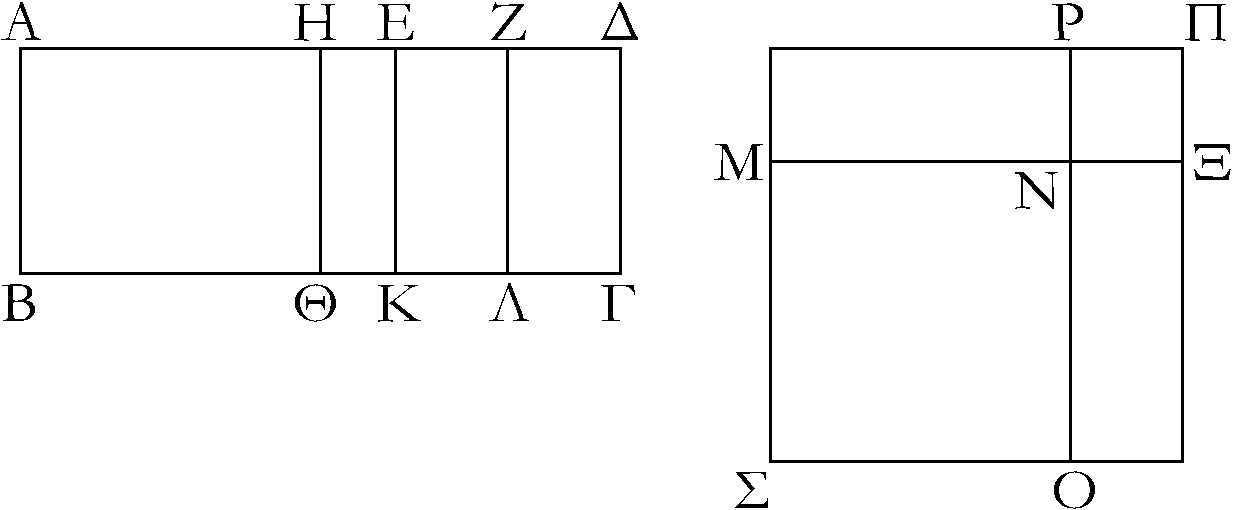
\includegraphics{Book10/fig054g.pdf}}

\gr{Ἐπεὶ
γὰρ ἀσύμμετρόξ ἐστιν ἡ ΑΗ τῆ| ΗΕ, ἀσύμμετ\-ρον >άρα ἐστὶ
καὶ τὸ ΑΘ τῶ| ΘΕ, τουτέστι τὸ ἀπὸ τῆξ ΜΝ τῶ| ἀπὸ
τῆξ ΝΧ; αἱ ΜΝ, ΝΧ >άρα δυνάμει εἰσὶν ἀσύμμετροι. καὶ
ἐπεὶ ἡ ΑΔ ἐκ δύο ὀνομάτων ἐστὶ πέμπτη, καί [ἐστιν]
>έλασσον α\kern -.7pt  ὐτῆξ τμ\kern -.7pt  ῆμα τὸ ΕΔ, σύμμετροξ >άρα ἡ ΕΔ τῆ| ΑΒ
μ\kern -.5pt  ήκει. ἀλλὰ ἡ ΑΕ τῆ| ΕΔ ἐστιν ἀσύμμετροξ; καὶ ἡ ΑΒ >άρα
τῆ| ΑΕ ἐστιν ἀσύμμετροξ μ\kern -.3pt  ήκει [αἱ ΒΑ, ΑΕ <ρηταί εἰσι δυνάμει
μόνον σύμμετροι]; μέσον >άρα ἐστὶ τὸ ΑΚ, τουτέστι τὸ συγκείμενον
ἐκ τῶν ἀπὸ τῶν ΜΝ, ΝΧ. καὶ ἐπεὶ σύμμετρόξ ἐστιν ἡ ΔΕ
τῆ| ΑΒ μ\kern -.7pt  ήκει, τουτέστι τῆ| ΕΚ, ἀλλὰ ἡ ΔΕ τῆ| ΕΖ σύμμετρόξ
ἐστιν, καὶ ἡ ΕΖ >άρα τῆ| ΕΚ σύμμετρόξ ἐστιν. καὶ <ρητὴ ἡ
ΕΚ; <ρητὸν >άρα καὶ τὸ ΕΛ, τουτέστι τὸ ΜΡ, τουτέστι τὸ ὑπὸ
ΜΝΧ; αἱ ΜΝ, ΝΧ >άρα δυνάμει ἀσύμμετροί εἰσι ποιοῦσαι
τὸ μὲν συγκείμενον ἐκ τῶν ἀπ> α\kern -.7pt  ὐτῶν τετραγώνων
μέσον, τὸ δ> ὑπ> α\kern -.7pt  ὐτῶν <ρητόν.}

\gr{Ἡ ΜΧ >άρα <ρητὸν καὶ μέσον δυναμένη ἐστὶ καὶ δύναται
τὸ ΑΓ θωρίον; <όπερ >έδει δεῖχαι.}}

\ParallelRText{
\begin{center}
{\large Proposition 58}
\end{center}

If an area is contained by a rational (straight-line)
and a fifth binomial (straight-line) then the square-root of the area is
the irrational (straight-line which is) called the square-root of a rational
plus a medial (area).$^\dag$

For let the area $AC$ be contained by the rational (straight-line) $AB$
and the fifth binomial (straight-line) $AD$, which has been divided into its
(component) terms at $E$, such that $AE$ is the greater term. [So] I say that
the square-root of area $AC$ is the irrational (straight-line which is)
called the square-root of a rational plus a medial (area).

For let the same construction  be made as that shown previously.
So, (it is) clear that $MO$ is the square-root of area $AC$.
So, we must show that $MO$ is the square-root of a rational plus a medial
(area).

% Removed epsf size command
\centerline{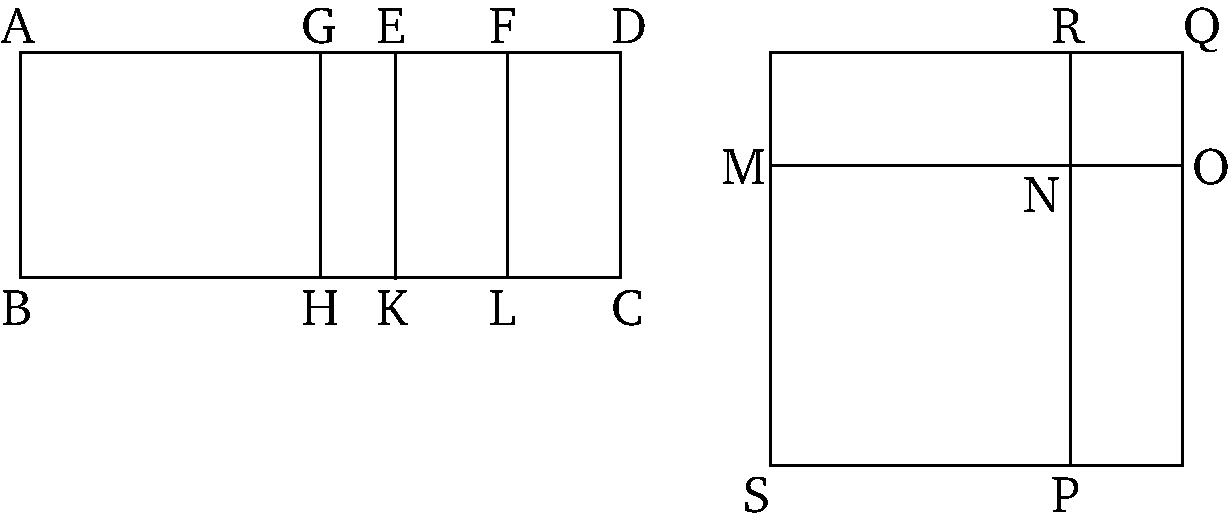
\includegraphics{Book10/fig054e.pdf}}

 For since $AG$ is incommensurable (in length) with $GE$ [Prop.~10.18], $AH$ is thus also
 incommensurable with $HE$---that is to say, the (square) on $MN$
 with the (square) on $NO$ [Props.~6.1, 10.11]. Thus, $MN$ and $NO$
 are incommensurable in square. And since $AD$ is a fifth
 binomial (straight-line), and $ED$ [is] its lesser segment, $ED$
 (is) thus commensurable in length with $AB$ [Def.~10.9]. But, $AE$ is incommensurable (in length) with $ED$. Thus, $AB$ is also incommensurable in length with $AE$
 [$BA$ and $AE$ are rational (straight-lines which are) commensurable
 in square only] [Prop.~10.13]. Thus, $AK$---that
 is to say, the sum of the (squares) on $MN$ and $NO$---is medial [Prop.~10.21]. And since $DE$ is
 commensurable in length with $AB$---that is to say, with $EK$---but,
 $DE$ is commensurable (in length) with $EF$, $EF$ is thus
also  commensurable (in length) with $EK$ [Prop.~10.12]. And $EK$ (is) rational. Thus, $EL$---that is to say, $MR$---that is to say, the (rectangle contained) by
$MNO$---(is) also rational [Prop.~10.19]. 
$MN$ and $NO$ are thus (straight-lines which are) incommensurable in square, making
the sum of the squares on them medial, and the (rectangle contained)
by them rational.

Thus, $MO$ is the square-root of a rational plus a medial (area) [Prop.~10.40]. And (it is) the square-root
of area $AC$. (Which is) the very thing it was required to show.}
\end{Parallel}
{\footnotesize\noindent $^\dag$
If the rational straight-line has unit length then this proposition states that the square-root of 
a fifth binomial straight-line is the square root of a rational plus a medial area: {i.e.}, 
a fifth binomial straight-line has a length $k\,(\sqrt{1+k'}+1)$ whose
square-root can be written\\ $\rho\,\sqrt{[(1+k''^{\,2})^{1/2}+k'']/[2\,(1+k''^{\,2})]}+\rho\,\sqrt{[(1+k''^{\,2})^{1/2}-k'']/[2\,(1+k''^{\,2})]}$, where $\rho=\sqrt{k\,(1+k''^{\,2})}$ and $k''^{\,2}=k'$. This is the length of the square root of a rational plus a medial area (see Prop.~10.40), since $\rho$ is rational.}

%%%%
%10.59
%%%%
\pdfbookmark[1]{Proposition 10.59}{pdf10.59}
\begin{Parallel}{}{}
\ParallelLText{
\begin{center}
{\large \ggn{59}.}
\end{center}\vspace*{-7pt}

\gr{Ἐὰν θωρίον περιέθηται ὑπὸ <ρητῆξ καὶ τῆξ ἐκ δύο ὀνομάτων
<έκτηξ, ἡ τὸ θωρίον δυναμένη >άλογόξ ἐστιν ἡ καλουμένη
δύο μέσα δυναμένη.}\\

% Removed epsf size command
\centerline{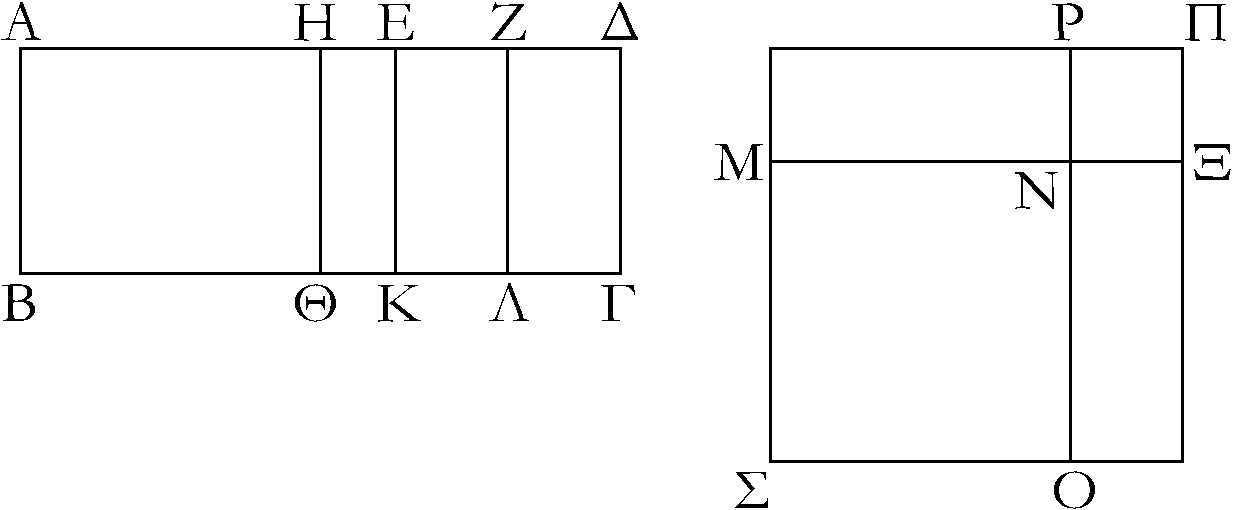
\includegraphics{Book10/fig054g.pdf}}

\gr{Θωρίον γὰρ τὸ ΑΒΓΔ περιεθέσθω ὑπὸ <ρητῆξ τῆξ ΑΒ καὶ τῆξ
ἐκ δύο ὀνομάτων <έκτηξ τῆξ ΑΔ διῃρημένηξ εἰξ τὰ ὀνόματα
κατὰ τὸ Ε, <ώστε τὸ μεῖζον >όνομα ε>ῖναι τὸ ΑΕ; λέγω, <ότι
ἡ τὸ ΑΓ δυναμένη ἡ δύο μέσα δυναμένη ἐστίν.}

\gr{Κατεσκευάσθω [γὰρ] τὰ α\kern -.7pt  ὐτὰ τοῖξ προδεδειγμένοιξ. φανερὸν δή,
<ότι [ἡ] τὸ ΑΓ δυναμένη ἐστὶν ἡ ΜΧ, καὶ <ότι ἀσύμμετρόξ ἐστιν
ἡ ΜΝ τῆ| ΝΧ δυνάμει. καὶ ἐπεὶ ἀσύμμετρόξ ἐστιν ἡ ΕΑ τῆ|
ΑΒ μ\kern -.7pt  ήκει, αἱ ΕΑ, ΑΒ >άρα <ρηταί εἰσι δυνάμει μόνον σύμμετροι; μέσον >άρα ἐστὶ τὸ ΑΚ, τουτέστι τὸ συγκείμενον ἐκ τῶν ἀπὸ
τῶν ΜΝ, ΝΧ. πάλιν, ἐπεὶ ἀσύμμετρόξ ἐστιν ἡ ΕΔ τῆ| ΑΒ μ\kern -.5pt  ήκει,
ἀσύμμετροξ >άρα ἐστὶ καὶ ἡ ΖΕ τῆ| ΕΚ; αἱ ΖΕ, ΕΚ >άρα
<ρηταί εἰσι δυνάμει μόνον σύμμετροι; μέσον >άρα ἐστὶ τὸ ΕΛ,
τουτέστι τὸ ΜΡ, τουτέστι τὸ ὑπὸ τῶν ΜΝΧ. καὶ ἐπεὶ ἀσύμμετροξ
ἡ ΑΕ τῆ| ΕΖ, καὶ τὸ ΑΚ τῶ| ΕΛ ἀσύμμετρόν ἐστιν. ἀλλὰ τὸ μὲν
ΑΚ ἐστι τὸ συγκείμενον ἐκ τῶν ἀπὸ τῶν ΜΝ, ΝΧ,
τὸ δὲ ΕΛ ἐστι τὸ ὑπὸ τῶν ΜΝΧ; ἀσύμμετρον >άρα ἐστὶ τὸ
συγκείμενον ἐκ τῶν ἀπὸ τῶν ΜΝΧ τῶ| ὑπὸ
τῶν ΜΝΧ. καί ἐστι μέσον ἑκάτερον α\kern -.3pt  ὐτῶν, καὶ αἱ ΜΝ, ΝΧ
δυνάμει εἰσὶν ἀσύμμετροι.}

\gr{Ἡ ΜΧ >άρα δύο μέσα δυναμένη ἐστὶ καὶ δύναται τὸ 
ΑΓ; <όπερ >έδει δεῖχαι.}}

\ParallelRText{
\begin{center}
{\large Proposition 59}
\end{center}

If an area is contained by a rational (straight-line)
and a sixth binomial (straight-line) then the square-root of the
area is the irrational (straight-line which is)  called the square-root
of (the sum of) two medial (areas).$^\dag$

% Removed epsf size command
\centerline{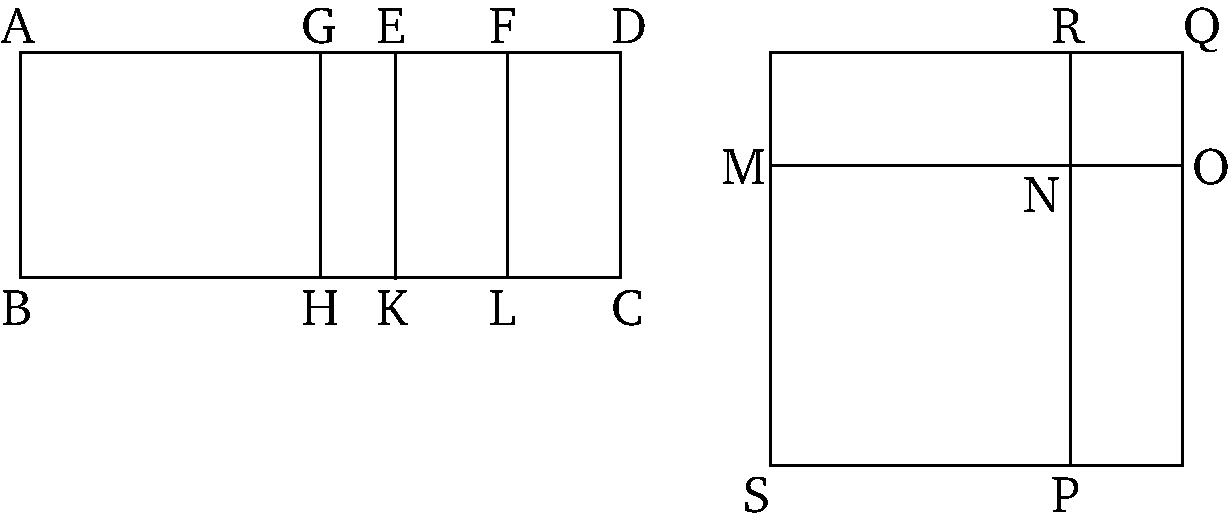
\includegraphics{Book10/fig054e.pdf}}

For let the area $ABCD$ be contained by the rational (straight-line)
$AB$ and the sixth binomial (straight-line) $AD$, which has been
divided into its (component) terms at $E$, such that $AE$ is the greater
term. So, I say that the square-root of $AC$ is the square-root
of (the sum of) two medial (areas).

\mbox{[}For] let the same construction  be made as that shown previously. So, (it is)
clear that $MO$ is the square-root of $AC$, and that $MN$ is incommensurable
in square with $NO$. And since $EA$ is incommensurable
in length with $AB$ [Def.~10.10], $EA$ and $AB$ are thus rational (straight-lines
which are) commensurable in square only. Thus, $AK$---that is to
say, the sum of the (squares) on $MN$ and $NO$---is medial [Prop.~10.21]. Again, since  $ED$ is incommensurable in length with $AB$  [Def.~10.10], $FE$ is thus also incommensurable 
(in length) with $EK$ [Prop.~10.13]. 
Thus, $FE$ and $EK$ are rational (straight-lines which are) commensurable
in square only. Thus, $EL$---that is to say,  $MR$---that is to say,
the (rectangle contained) by $MNO$---is medial [Prop.~10.21]. And since $AE$ is incommensurable
(in length) with $EF$, $AK$ is also incommensurable with $EL$
[Props.~6.1, 10.11]. 
But, $AK$ is the sum of the (squares) on $MN$ and $NO$, and $EL$
is the (rectangle contained) by $MNO$. Thus,
the sum of the (squares) on $MNO$ is incommensurable with the (rectangle
contained) by $MNO$. And each of them is medial.  And $MN$ and
$NO$ are incommensurable in square.

Thus, $MO$ is the square-root of (the sum of) two medial (areas) [Prop.~10.41].
And (it is) the square-root of $AC$. (Which is) the very thing it was required
to show.}
\end{Parallel}
{\footnotesize\noindent$^\dag$ If the rational straight-line has unit length then this proposition states that the square-root of 
a sixth binomial straight-line is the square root of the sum of  two  medial areas: {i.e.}, 
a sixth binomial straight-line has a length $\sqrt{k}+\sqrt{k'}$ whose
square-root can be written\\ $k^{1/4}\left(\sqrt{[1+k''/(1+k''^{\,2})^{1/2}]/2}+\sqrt{[1-k''/(1+k''^{\,2})^{1/2}]/2}\right)$, where $k''^{\,2}=(k-k')/k'$. This is the length of the square-root of the sum of two medial areas (see Prop.~10.41).}

%%%%
%10.59a
%%%%
\begin{Parallel}{}{}
\ParallelLText{
\begin{center}
{\large \gr{Λῆμμα}.}
\end{center}\vspace*{-7pt}

\gr{Ἐὰν εὐθεῖα γραμμ\kern -.7pt  ὴ τμ\kern -.7pt  ηθῆ| εἰξ >άνισα, τὰ ἀπὸ τῶν ἀνίσων
τετράγωνα μείζονά ἐστι τοῦ δὶξ ὑπὸ τῶν ἀνίσων περιεθομένου
ὀρθογωνίου.}

% Removed epsf size command
\centerline{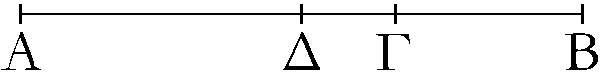
\includegraphics{Book10/fig059ag.pdf}}

\gr{>'Εστω εὐθεῖα ἡ ΑΒ καὶ τετμ\kern -.7pt  ήσθω εἰξ >άνισα κατὰ τὸ Γ, καὶ >έστω
μείζων ἡ ΑΓ; λέγω, <ότι τὰ ἀπὸ τῶν ΑΓ, ΓΒ μείζονά ἐστι
τοῦ δὶξ ὑπὸ τῶν ΑΓ, ΓΒ.}

\gr{Τετμ\kern -.7pt  ήσθω γὰρ ἡ ΑΒ δίθα κατὰ τὸ Δ. ἐπεὶ ο>ῦν εὐθεῖα
γραμμ\kern -.7pt  ὴ τέτμ\kern -.5pt  ηται εἰξ μὲν >ίσα κατὰ τὸ Δ, εἰξ
δὲ >άνισα κατὰ τὸ Γ, τὸ >άρα ὑπὸ τῶν ΑΓ, ΓΒ μετὰ
τοῦ ἀπὸ ΓΔ >ίσον ἐστὶ τῶ| ἀπὸ ΑΔ; <ώστε τὸ ὑπὸ
τῶν ΑΓ, ΓΒ >έλαττόν ἐστι τοῦ ἀπὸ ΑΔ; τὸ >άρα δὶξ
ὑπὸ τῶν ΑΓ, ΓΒ >έλαττον
 >ὴ διπλάσιόν ἐστι τοῦ ἀπὸ
ΑΔ. ἀλλὰ τὰ ἀπὸ τῶν ΑΓ, ΓΒ διπλάσιά [ἐστι] τῶν
ἀπὸ τῶν ΑΔ, ΔΓ; τὰ >άρα ἀπὸ τῶν ΑΓ, ΓΒ μείζονά
ἐστι τοῦ δὶξ ὑπὸ τῶν ΑΓ, ΓΒ; <όπερ >έδει δεῖχαι.}}

\ParallelRText{
\begin{center}
{\large Lemma}
\end{center}

If a straight-line is cut unequally then 
(the sum of) the squares on the unequal (parts) is greater than twice
the rectangle contained by the unequal (parts).

% Removed epsf size command
\centerline{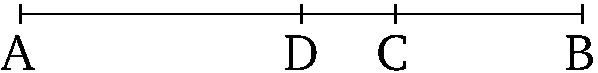
\includegraphics{Book10/fig059ae.pdf}}

Let $AB$ be a straight-line, and let it be cut unequally at $C$, and
let $AC$ be greater (than $CB$). I say that (the sum of) the (squares) on
$AC$ and $CB$ is greater than twice the (rectangle contained) by $AC$ and
$CB$.

For let $AB$ be cut in half at $D$. Therefore, since a straight-line
has been cut into equal (parts) at $D$, and into unequal (parts) at $C$,
 the (rectangle contained) by $AC$ and $CB$, plus the (square)
on $CD$, is thus equal to the (square) on $AD$ [Prop.~2.5]. Hence, the (rectangle contained) by $AC$ and $CB$ is less than the (square) on $AD$. Thus, twice the
(rectangle contained) by $AC$ and $CB$ is less than double the (square) on
$AD$. But, (the sum of) the (squares) on $AC$ and $CB$ [is] double (the sum of) the (squares) on $AD$ and $DC$ [Prop.~2.9].
Thus, (the sum of) the (squares) on $AC$ and $CB$ is greater than twice
the (rectangle contained) by $AC$ and $CB$. (Which is) the very thing it
was required to show.}
\end{Parallel}

%%%%
%10.60
%%%%
\pdfbookmark[1]{Proposition 10.60}{pdf10.60}
\begin{Parallel}{}{}
\ParallelLText{
\begin{center}
{\large \ggn{60}.}
\end{center}\vspace*{-7pt}

\gr{Τὸ ἀπὸ τῆξ ἐκ δύο ὀνομάτων παρὰ <ρητὴν  παραβαλλόμενον πλάτοξ
ποιεῖ τὴν ἐκ δύο ὀνομάτων πρώτην.}\\

% Removed epsf size command
\centerline{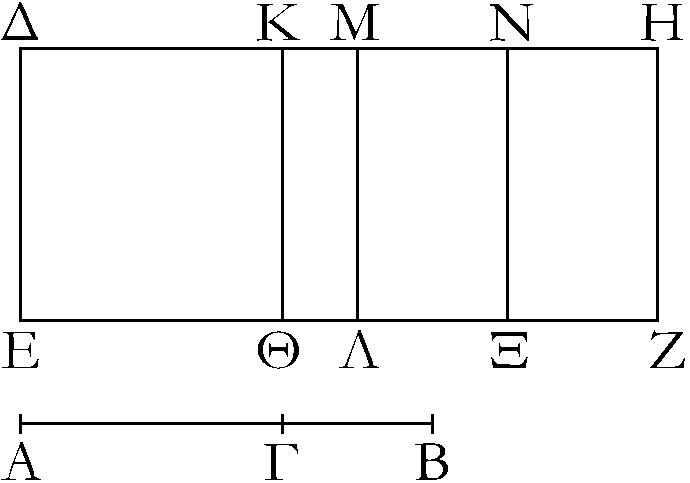
\includegraphics{Book10/fig060g.pdf}}

\gr{>'Εστω ἐκ δύο ὀνομάτων ἡ ΑΒ διῃρημένη εἰξ τὰ ὀνόματα κατὰ
τὸ Γ, <ώστε τὸ μεῖζον >όνομα ε>ῖναι τὸ ΑΓ, καὶ ἐκκείσθω
<ρητὴ ἡ ΔΕ, καὶ τῶ| ἀπὸ τῆξ ΑΒ >ίσον παρὰ τὴν ΔΕ παραβεβλήσθω
τὸ ΔΕΖΗ πλάτοξ ποιοῦν τὴν ΔΗ; λέγω, <ότι ἡ ΔΗ ἐκ δύο ὀνομάτων
ἐστὶ πρώτη.}

\gr{Παραβεβλήσθω γὰρ παρὰ τὴν ΔΕ τῶ| μὲν ἀπὸ τῆξ ΑΓ >ίσον τὸ ΔΘ,
τῶ| δὲ ἀπὸ τῆξ ΒΓ >ίσον τὸ ΚΛ; λοιπὸν >άρα τὸ δὶξ ὑπὸ τῶν
ΑΓ, ΓΒ >ίσον ἐστὶ τῶ| ΜΖ. τετμ\kern -.7pt  ήσθω ἡ ΜΗ δίθα κατὰ τὸ Ν, καὶ
παράλληλοξ >ήθθω ἡ ΝΧ [ἑκατέρᾳ τῶν ΜΛ, ΗΖ]. ἑκάτερον >άρα
τῶν ΜΧ, ΝΖ >ίσον ἐστὶ τῶ| <άπαχ ὑπὸ τῶν ΑΓΒ. καὶ ἐπεὶ
ἐκ δύο ὀνομάτων ἐστὶν ἡ ΑΒ διῃρημένη εἰξ τὰ ὀνόματα
κατὰ τὸ Γ, αἱ ΑΓ, ΓΒ >άρα <ρηταί εἰσι δυνάμει μόνον σύμμετροι;
τὰ >άρα ἀπὸ τῶν ΑΓ, ΓΒ <ρητά ἐστι καὶ σύμμετρα ἀλλήλοιξ;
<ώστε καὶ τὸ συγκείμενον ἐκ τῶν ἀπὸ τῶν ΑΓ, ΓΒ.
καί ἐστιν >ίσον τῶ| ΔΛ; <ρητὸν >άρα
ἐστὶ τὸ ΔΛ. καὶ παρὰ <ρητὴν τὴν ΔΕ παράκειται; <ρητὴ >άρα ἐστὶν
ἡ ΔΜ καὶ σύμμετροξ τῆ| ΔΕ μ\kern -.7pt  ήκει. πάλιν, ἐπεὶ αἱ ΑΓ, ΓΒ <ρηταί
εἰσι δυνάμει μόνον σύμμετροι, μέσον >άρα ἐστὶ τὸ δὶξ ὑπὸ
τῶν ΑΓ, ΓΒ, τουτέστι τὸ ΜΖ. καὶ παρὰ <ρητὴν τὴν ΜΛ παράκειται;
<ρητὴ >άρα καὶ ἡ ΜΗ καὶ ἀσύμμετροξ τῆ| ΜΛ, τουτέστι
τῆ| ΔΕ, μ\kern -.5pt  ήκει. >έστι δὲ καὶ ἡ ΜΔ <ρητὴ καὶ τῆ| ΔΕ μ\kern -.3pt  ήκει
σύμμετροξ; ἀσύμμετροξ >άρα ἐστὶν ἡ ΔΜ τῆ| ΜΗ μ\kern -.7pt  ήκει. καί εἰσι
<ρηταί; αἱ ΔΜ, ΜΗ >άρα <ρηταί εἰσι δυνάμει μόνον σύμμετροι;
ἐκ δύο >άρα ὀνομάτων ἐστὶν ἡ ΔΗ. δεικτέον δή, <ότι
καὶ πρώτη.}

\gr{Ἐπεὶ τῶν ἀπὸ τῶν ΑΓ, ΓΒ μέσον ἀνάλογόν ἐστι τὸ ὑπὸ τῶν
ΑΓΒ, καὶ τῶν ΔΘ, ΚΛ >άρα μέσον ἀνάλογόν ἐστι τὸ ΜΧ. >έστιν
>άρα ὡξ τὸ ΔΘ πρὸξ τὸ ΜΧ, ο<ύτωξ τὸ ΜΧ πρὸξ τὸ
ΚΛ, τουτέστιν ὡξ ἡ ΔΚ πρὸξ τὴν ΜΝ, ἡ ΜΝ πρὸξ τὴν ΜΚ;
τὸ >άρα ὑπὸ τῶν ΔΚ, ΚΜ >ίσον ἐστὶ τῶ| ἀπὸ τῆξ ΜΝ.
καὶ ἐπεὶ σύμμετρόν ἐστι τὸ ἀπὸ τῆξ ΑΓ τῶ| ἀπὸ τῆξ ΓΒ,
σύμμετρόν ἐστι καὶ τὸ ΔΘ τῶ| ΚΛ; <ώστε καὶ ἡ ΔΚ τῆ|
ΚΜ σύμμετρόξ ἐστιν. καὶ ἐπεὶ μείζονά ἐστι τὰ ἀπὸ τῶν ΑΓ,
ΓΒ τοῦ δὶξ ὑπὸ τῶν ΑΓ, ΓΒ, μεῖζον >άρα καὶ τὸ ΔΛ τοῦ
ΜΖ; <ώστε καὶ ἡ ΔΜ τῆξ ΜΗ μείζων ἐστίν. καί ἐστιν >ίσον
τὸ ὑπὸ τῶν ΔΚ, ΚΜ τῶ| ἀπὸ τῆξ ΜΝ, τουτέστι τῶ| τετάρτῳ
 τοῦ ἀπὸ τῆξ ΜΗ  -.7πτ η, καὶ σύμμετροξ ἡ ΔΚ τῆ| ΚΜ. ἒαν
δὲ >ῶσι δύο εὐθεῖαι >άνισοι,  τῶ| δὲ τετάρτῳ μέρει τοῦ ἀπὸ τῆξ
ἐλάσσονοξ >ίσον παρὰ τὴν μείζονα παραβληθῆ| ἐλλεῖπον
ε>ίδει τετραγώνῳ  καὶ εἰξ σύμμετρα α\kern -.7pt  ὐτὴν διαιρῆ|, ἡ μείζων
τῆξ ἐλάσσονοξ μεῖζον δύναται τῶ| ἀπὸ συμμέτρου ἑαυτῆ|; ἡ
ΔΜ >άρα τῆξ ΜΗ μεῖζον δύναται τῶ| ἀπὸ συμμέτρου
ἑαυτῆ|. καί εἰσι <ρηταὶ αἱ ΔΜ, ΜΗ , καὶ ἡ ΔΜ μεῖζον
>όνομα ο>ῦσα σύμμετρόξ ἐστι τῆ| ἐκκειμένῃ <ρητῆ| τῆ|
ΔΕ μ\kern -.7pt  ήκει.}

\gr{Ἡ ΔΗ >άρα ἐκ δύο ὀνομάτων ἐστὶ πρώτη; <όπερ >έδει
δεῖχαι.}}

\ParallelRText{
\begin{center}
{\large Proposition 60}
\end{center}

The square on a binomial (straight-line) applied to a rational (straight-line) produces as breadth a first binomial (straight-line).$^\dag$

% Removed epsf size command
\centerline{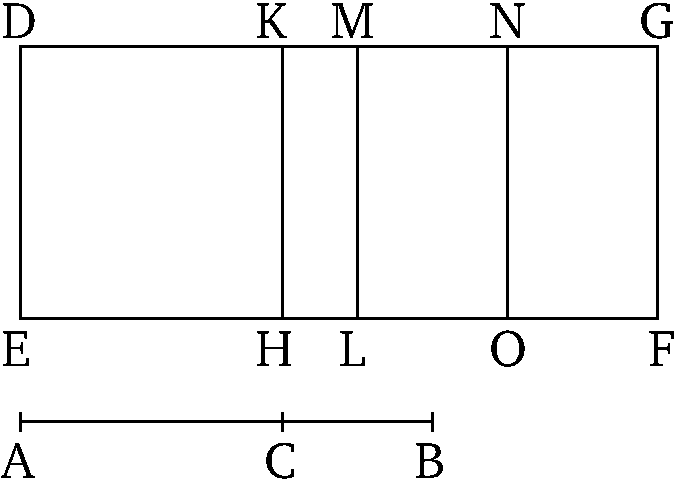
\includegraphics{Book10/fig060e.pdf}}

Let $AB$ be a binomial (straight-line), having been divided into its
(component) terms at $C$, such that $AC$ is the greater term. And let the
rational (straight-line) $DE$ be laid down. And let the (rectangle)
$DEFG$, equal to the (square) on $AB$, be applied to $DE$,
producing $DG$ as breadth. I say that $DG$ is a first binomial (straight-line).

For let $DH$, equal to the (square) on $AC$,  and $KL$, equal to the
(square) on $BC$, be applied to $DE$. Thus, the remaining twice
the (rectangle contained) by $AC$ and $CB$ is equal to $MF$ [Prop.~2.4].  Let $MG$ be cut in half
at $N$, and let $NO$ be drawn parallel [to each of $ML$ and
$GF$]. $MO$ and $NF$ are thus each equal to once the (rectangle contained)
by $ACB$. And since $AB$ is a binomial (straight-line), having been divided into its (component) terms at $C$,  $AC$ and $CB$ are thus rational (straight-lines which are) commensurable in square only [Prop.~10.36]. Thus, the (squares) on $AC$ and $CB$ are rational, and commensurable with one another.  And hence the
sum of the (squares) on $AC$ and $CB$ (is rational) [Prop.~10.15], and is equal to $DL$. Thus, $DL$
is rational. And it is applied to the rational (straight-line) $DE$. $DM$
is thus rational, and commensurable in length with $DE$ [Prop.~10.20]. Again, since $AC$ and $CB$
are rational (straight-lines which are) commensurable in square only, twice the (rectangle contained) by $AC$ and $CB$---that is to say, $MF$---is thus medial [Prop.~10.21]. And it is applied to the
rational (straight-line) $ML$. $MG$ is thus also rational, and incommensurable in length with $ML$---that is to say, with $DE$
[Prop.~10.22].  And $MD$ is also rational, and
commensurable in length with $DE$. Thus, $DM$ is  incommensurable in length with $MG$ [Prop.~10.13]. And
they are rational. $DM$ and $MG$ are thus rational (straight-lines which
are) commensurable in square only. Thus, $DG$ is a binomial (straight-line)
[Prop.~10.36]. So, we must show that (it is)
also a first (binomial straight-line).

Since the (rectangle contained) by $ACB$ is the mean proportional to
 the squares on $AC$ and $CB$ [Prop.~10.53~lem.], $MO$ is thus also the
mean proportional to   $DH$ and $KL$. Thus,
as $DH$ is to $MO$, so $MO$ (is) to $KL$---that is to say, as $DK$
(is) to $MN$, (so) $MN$ (is) to $MK$ [Prop.~6.1].
Thus, the (rectangle contained) by $DK$ and $KM$ is equal
to the (square) on $MN$ [Prop.~6.17]. And since
the (square) on $AC$ is commensurable with the (square) on $CB$,
$DH$ is also commensurable with $KL$. Hence, $DK$
is also commensurable with $KM$ [Props.~6.1, 10.11].
And since (the sum of) the squares on $AC$ and $CB$ is greater
than twice the (rectangle contained) by $AC$ and $CB$ [Prop.~10.59~lem.], $DL$ (is) thus also
greater than $MF$. Hence, $DM$ is also greater than $MG$
[Props.~6.1, 5.14]. And
the (rectangle contained) by $DK$ and $KM$ is equal to
the (square) on $MN$---that is to say, to one quarter the (square) on $MG$.
And $DK$ (is) commensurable (in length) with $KM$. And if there are
two unequal straight-lines, and a (rectangle) equal to the fourth part
of the (square) on the lesser, falling short by a square figure, is applied to
the greater, and divides it into (parts which are) commensurable (in length),
then the square on the greater is larger than (the square on) the lesser by
the (square) on (some straight-line) commensurable (in length) with the greater [Prop.~10.17]. Thus,  the square on $DM$
is greater than (the square on) $MG$ by the (square) on (some straight-line)
commensurable (in length) with ($DM$). And $DM$ and $MG$ are rational. And
$DM$, which is the greater term, is commensurable in length with the (previously) laid down rational (straight-line) $DE$.

Thus, $DG$ is a first binomial (straight-line) [Def.~10.5]. (Which is) the very thing it was required to show.}
\end{Parallel}
{\footnotesize\noindent$^\dag$ In other words, the square of a binomial  is a
first binomial. See Prop.~10.54.}

%%%%
%10.61
%%%%
\pdfbookmark[1]{Proposition 10.61}{pdf10.61}
\begin{Parallel}{}{}
\ParallelLText{
\begin{center}
{\large \ggn{61}.}
\end{center}\vspace*{-7pt}

\gr{Τὸ ἀπὸ τῆξ ἐκ δύο μέσων πρώτηξ παρὰ <ρητὴν παραβαλλόμενον πλάτοξ ποιεῖ τὴν ἐκ δύο ὀνομάτων δευτέραν.}

\gr{>'Εστω ἐκ δύο μέσων πρώτη ἡ ΑΒ διῃρημένη εἰξ τὰξ μέσαξ κατὰ
τὸ Γ, <ῶν μείζων ἡ ΑΓ, καὶ ἐκκείσθω <ρητὴ ἡ ΔΕ, καὶ παραβεβλήσθω παρὰ τὴν ΔΕ τῶ| ἀπὸ τῆξ ΑΒ >ίσον παραλληλόγραμμον
τὸ ΔΖ πλάτοξ ποιοῦν τὴν ΔΗ; λέγω, <ότι ἡ ΔΗ ἐκ δύο ὀνομάτων ἐστὶ δευτέρα.}

\gr{Κατεσκευάσθω γὰρ τὰ α\kern -.7pt  ὐτὰ τοῖξ πρὸ τούτου. καὶ ἐπεὶ ἡ ΑΒ
ἐκ δύο μέσων ἐστὶ πρώτη διῃρημένη κατὰ τὸ Γ, αἱ ΑΓ, ΓΒ >άρα
μέσαι εἰσὶ δυνάμει μόνον σύμμετροι <ρητὸν περιέθουσαι; <ώστε
καὶ τὰ ἀπὸ τῶν ΑΓ, ΓΒ μέσα ἐστίν. μέσον >άρα ἐστὶ τὸ ΔΛ.
καὶ παρὰ <ρητὴν τὴν ΔΕ παραβέβληται; <ρητὴ >άρα ἐστίν ἡ ΜΔ
καὶ ἀσύμμετροξ τῆ| ΔΕ μ\kern -.7pt  ήκει. πάλιν, ἐπεὶ <ρητόν ἐστι τὸ δὶξ
ὑπὸ τῶν ΑΓ, ΓΒ, <ρητόν ἐστι καὶ τὸ ΜΖ. καὶ παρὰ <ρητὴν τὴν
ΜΛ παράκειται; <ρητὴ >άρα [ἐστὶ] καὶ ἡ ΜΗ καὶ μ\kern -.5pt  ήκει σύμμετροξ
τῆ| ΜΛ, τουτέστι τῆ| ΔΕ; ἀσύμμετροξ >άρα ἐστὶν ἡ ΔΜ τῆ|
ΜΗ  μ\kern -.3pt  ήκει. καί εἰσι <ρηταί; αἱ ΔΜ, ΜΗ >άρα <ρηταί εἰσι δυνάμει
μόνον σύμμετροι; ἐκ δύο >άρα ὀνομάτων ἐστὶν ἡ ΔΗ. δεικτέον
δή, <ότι καὶ δευτέρα.}\\~\\~\\~\\~\\~\\~\\~\\

% Removed epsf size command
\centerline{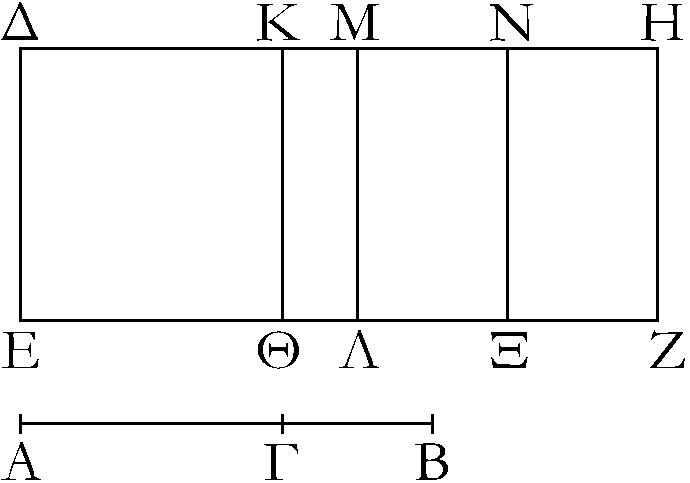
\includegraphics{Book10/fig060g.pdf}}

\gr{Ἐπεὶ γὰρ τὰ ἀπὸ τῶν ΑΓ, ΓΒ μείζονά ἐστι τοῦ δὶξ ὑπὸ τῶν
ΑΓ, ΓΒ, μεῖζον >άρα καὶ τὸ ΔΛ τοῦ ΜΖ; <ώστε καὶ ἡ ΔΜ τῆξ
ΜΗ . καὶ ἐπεὶ σύμμετρόν ἐστι τὸ ἀπὸ τῆξ ΑΓ τῶ| ἀπὸ τῆξ
ΓΒ, σύμμετρόν ἐστι καὶ τὸ ΔΘ τῶ| ΚΛ; <ώστε καὶ ἡ ΔΚ τῆ| ΚΜ
σύμμετρόξ ἐστιν. καί ἐστι τὸ ὑπὸ τῶν ΔΚΜ >ίσον τῶ| ἀπὸ
τῆξ ΜΝ; ἡ ΔΜ >άρα τῆξ ΜΗ μεῖζον δύναται τῶ| ἀπὸ συμμέτρου
ἑαυτῆ|. καί ἐστιν ἡ ΜΗ σύμμετροξ τῆ| ΔΕ μ\kern -.7pt  ήκει.}

\gr{Ἡ ΔΗ >άρα ἐκ δύο ὀνομάτων ἐστὶ δευτέρα.}}

\ParallelRText{
\begin{center}
{\large Proposition 61}
\end{center}

The square on a first bimedial (straight-line)
applied to a rational (straight-line) produces as breadth a second binomial
(straight-line).$^\dag$

Let $AB$ be a first bimedial (straight-line) having been divided into its (component)
medial (straight-lines) at $C$, of which $AC$ (is) the greater. And let
the rational (straight-line) $DE$ be laid down. And let the parallelogram
$DF$, equal to the (square) on $AB$, be applied to $DE$, producing
$DG$ as breadth. I say that $DG$ is a second binomial (straight-line).

For let the same construction be made as in the (proposition) before
this. And since $AB$ is a first bimedial (straight-line), having been divided at $C$, 
$AC$ and $CB$ are thus medial (straight-lines) commensurable
in square only, and containing a rational (area) [Prop.~10.37]. Hence, the (squares) on $AC$ and
$CB$ are also medial [Prop.~10.21]. Thus,
$DL$ is medial [Props.~10.15, 10.23~corr.].  And it has been applied to the
rational (straight-line) $DE$. $MD$ is thus rational, and incommensurable
in length with $DE$ [Prop.~10.22]. Again,
since twice the (rectangle contained) by $AC$ and $CB$ is rational,
$MF$ is also rational. And it is applied to the rational (straight-line)
$ML$. Thus, $MG$ [is] also rational, and commensurable in length
with $ML$---that is to say, with $DE$ [Prop.~10.20]. $DM$ is thus incommensurable in length with $MG$ [Prop.~10.13]. And they are rational. $DM$ and $MG$ are thus rational, and commensurable in square only. $DG$ is thus a binomial (straight-line) [Prop.~10.36]. So, we must show that (it
is) also a second (binomial straight-line).

% Removed epsf size command
\centerline{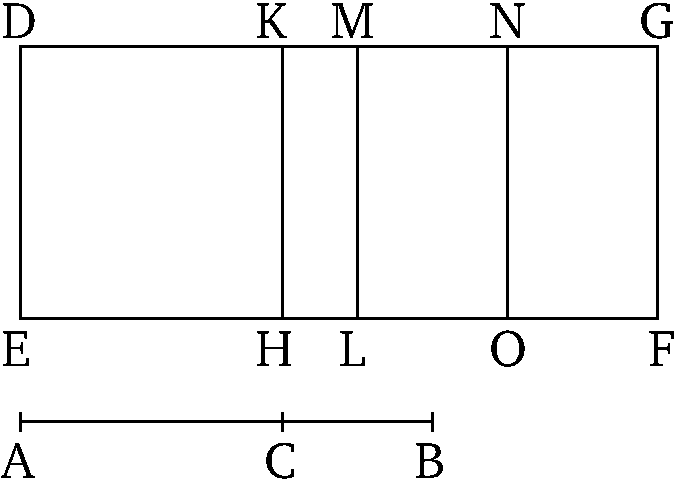
\includegraphics{Book10/fig060e.pdf}}

For since (the sum of) the squares on $AC$ and $CB$ is greater than twice
the (rectangle contained) by $AC$ and $CB$ [Prop.~10.59], $DL$ (is) thus also greater
than $MF$. Hence, $DM$ (is) also (greater) than $MG$ [Prop.~6.1]. And since
the (square) on $AC$ is commensurable with the (square) on $CB$, $DH$
is also commensurable with $KL$. Hence, $DK$ is also commensurable
(in length) with $KM$ [Props.~6.1, 10.11].  And the (rectangle contained) by $DKM$
is equal to the (square) on $MN$. Thus, the square on $DM$ is greater
than (the square on) $MG$ by the (square) on (some straight-line)
commensurable (in length) with ($DM$) [Prop.~10.17]. And $MG$ is commensurable in length
with $DE$.

Thus, $DG$ is a second binomial (straight-line) [Def. 10.6].}
\end{Parallel}
{\footnotesize\noindent $^\dag$In other words, the square of a first bimedial is a
second binomial. See Prop.~10.55.}

%%%%
%10.62
%%%%
\pdfbookmark[1]{Proposition 10.62}{pdf10.62}
\begin{Parallel}{}{}
\ParallelLText{
\begin{center}
{\large \ggn{62}.}
\end{center}\vspace*{-7pt}

\gr{Τὸ ἀπὸ τῆξ ἐκ δύο μέσων δευτέραξ παρὰ <ρητὴν παραβαλλόμενον
πλάτοξ ποιεῖ τὴν ἐκ δύο ὀνομάτων τρίτην.}

\gr{>'Εστω ἐκ δύο μέσων δευτέρα ἡ ΑΒ διῃρημένη εἰξ τὰξ μέσαξ
κατὰ τὸ Γ, <ώστε τὸ μεῖζον τμ\kern -.7pt  ῆμα ε>ῖναι τὸ ΑΓ, <ρητὴ δέ τιξ
>έστω ἡ ΔΕ, καὶ παρὰ τὴν ΔΕ τῶ| ἀπὸ τῆξ ΑΒ >ίσον παραλληλόγραμμον παραβεβλήσθω τὸ ΔΖ πλάτοξ ποιοῦν τὴν ΔΗ;
λέγω, <ότι ἡ ΔΗ ἐκ δύο ὀνομάτων ἐστὶ τρίτη.}

\gr{Κατεσκευάσθω τὰ α\kern -.7pt  ὐτὰ τοῖξ προδεδειγμένοιξ. καὶ ἐπεὶ ἐκ δύο
μέσων δευτέρα ἐστὶν ἡ ΑΒ διῃρημένη κατὰ τὸ Γ, αἱ ΑΓ, ΓΒ
>άρα μέσαι εἰσὶ δυνάμει μόνον σύμμετροι μέσον
περιέθουσαι; <ώστε καὶ τὸ συγκείμενον ἐκ τῶν ἀπὸ τῶν ΑΓ, ΓΒ
μέσον ἐστίν. καί ἐστιν >ίσον τῶ| ΔΛ; μέσον >άρα καὶ τὸ ΔΛ.
καὶ παράκειται παρὰ <ρητὴν τὴν ΔΕ; <ρητὴ >άρα ἐστὶ καὶ ἡ
ΜΔ καὶ ἀσύμμετροξ τῆ| ΔΕ μ\kern -.7pt  ήκει. διὰ τὰ α\kern -.5pt  ὐτὰ δὴ καὶ ἡ
ΜΗ  <ρητή ἐστι καὶ ἀσύμμετροξ τῆ| ΜΛ, τουτέστι τῆ| ΔΕ, μ\kern -.3pt  ήκει; <ρητὴ
>άρα ἐστὶν ἑκατέρα τῶν ΔΜ, ΜΗ καὶ ἀσύμμετροξ τῆ| ΔΕ μ\kern -.7pt  ήκει.
καὶ ἐπεὶ ἀσύμμετρόξ ἐστιν ἡ ΑΓ τῆ| ΓΒ μ\kern -.7pt  ήκει, ὡξ
δὲ ἡ ΑΓ πρὸξ τὴν ΓΒ, ο<ύτωξ τὸ ἀπὸ τῆξ ΑΓ πρὸξ τὸ ὑπὸ τῶν
ΑΓΒ, ἀσύμμετρον >άρα καὶ τὸ ἀπὸ τῆξ ΑΓ τῶ| ὑπὸ
τῶν ΑΓΒ. <ώστε καὶ τὸ συγκείμενον ἐκ τῶν ἀπὸ τῶν ΑΓ, ΓΒ
τῶ| δὶξ ὑπὸ τῶν ΑΓΒ ἀσύμμετρόν ἐστιν, τουτέστι τὸ ΔΛ τῶ|
ΜΖ;  <ώστε καὶ ἡ ΔΜ τῶ| ΜΗ ἀσύμμετρόξ ἐστιν. καί εἰσι
<ρηταί; ἐκ δύο >άρα ὀνομάτων ἐστὶν ἡ ΔΗ. δεικτέον
[δή], <ότι καὶ τρίτη.}\\~\\~\\~\\~\\~\\~\\~\\~\\

% Removed epsf size command
\centerline{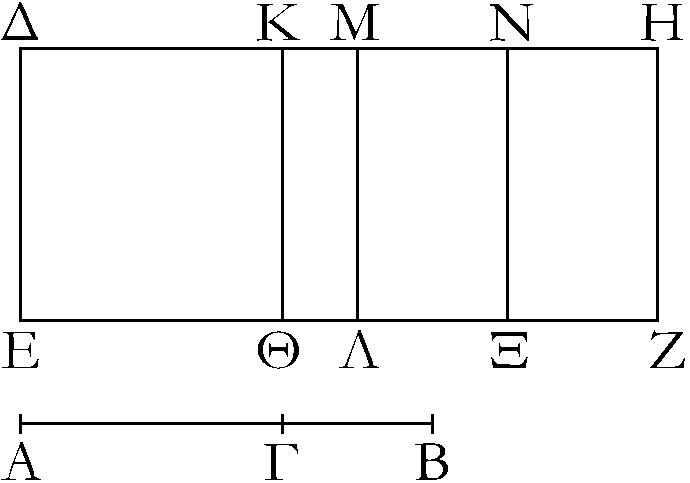
\includegraphics{Book10/fig060g.pdf}}

\gr{Ὁμοίωξ δὴ τοῖξ προτέροιξ ἐπιλογιούμεθα, <ότι μείζων ἐστὶν ἡ ΔΜ
τῆξ ΜΗ , καὶ σύμμετροξ ἡ ΔΚ τῆ| ΚΜ. καί ἐστι τὸ ὑπὸ τῶν
ΔΚΜ >ίσον τῶ| ἀπὸ τῆξ ΜΝ; ἡ ΔΜ >άρα τῆξ ΜΗ μεῖζον
δύναται τῶ| ἀπὸ συμμέτρου ἑαυτῆ|. καὶ οὐδετέρα τῶν ΔΜ, ΜΗ 
σύμμετρόξ ἐστι τῆ| ΔΕ μ\kern -.7pt  ήκει.}

\gr{Ἡ ΔΗ >άρα ἐκ δύο ὀνομάτων ἐστὶ τρίτη; <όπερ >έδει
δεῖχαι.}}

\ParallelRText{
\begin{center}
{\large Proposition 62}
\end{center}

The square on a second bimedial (straight-line)
applied to  a rational (straight-line) produces as breadth a third binomial
(straight-line).$^\dag$

Let $AB$ be a second bimedial (straight-line) having been divided into its (component)
medial (straight-lines) at $C$, such that $AC$ is the greater segment. And
let $DE$ be some rational (straight-line). And let the parallelogram
$DF$, equal to the (square) on $AB$, be applied to $DE$,
producing $DG$ as breadth. I say that $DG$ is a third binomial (straight-line).

Let the same construction  be made as that shown previously. And since $AB$ is a second bimedial (straight-line), having been divided at $C$, $AC$ and
$CB$ are thus medial (straight-lines) commensurable in square only,
and containing a medial (area) [Prop.~10.38]. Hence, the sum  of the (squares) on
$AC$ and $CB$ is also medial [Props.~10.15, 10.23~corr.]. And it is equal to $DL$. Thus, $DL$ (is)
also medial. And it is applied to the rational (straight-line) $DE$. $MD$
is thus also rational, and incommensurable in length with $DE$
[Prop.~10.22]. So, for the same (reasons),
$MG$ is also rational, and incommensurable in length with $ML$---that is to say, with $DE$. Thus, $DM$ and $MG$ are each rational, and incommensurable in length with $DE$. And since	$AC$ is incommensurable
in length with $CB$, and as $AC$ (is) to $CB$, so the (square)
on $AC$ (is) to the (rectangle contained) by $ACB$ [Prop.~10.21~lem.], the (square) on $AC$
(is) also incommensurable with the (rectangle contained) by $ACB$
[Prop.~10.11]. And hence the sum of the
(squares) on $AC$ and $CB$ is incommensurable with twice the (rectangle
contained) by $ACB$---that is to say, $DL$ with $MF$ [Props.~10.12, 10.13].  Hence,
$DM$ is also incommensurable (in length) with $MG$ [Props.~6.1, 10.11].
And they are rational.  $DG$ is thus a binomial (straight-line)
[Prop.~10.36]. [So]
we must show that (it is) also a third (binomial straight-line).

% Removed epsf size command
\centerline{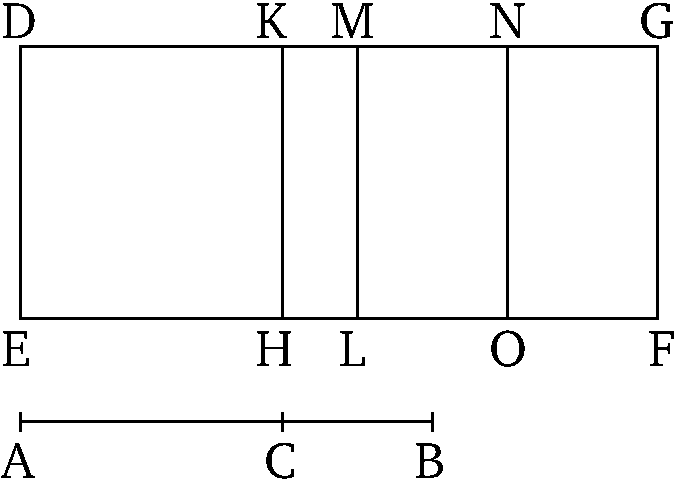
\includegraphics{Book10/fig060e.pdf}}

So, similarly to the previous (propositions), we can conclude that
$DM$ is greater than $MG$, and $DK$ (is) commensurable (in length) 
with $KM$.  And the (rectangle contained) by $DKM$ is equal to the
(square) on $MN$. Thus, the square on $DM$ is greater than (the square on)
$MG$ by the (square) on (some straight-line) commensurable (in length) with ($DM$)
[Prop.~10.17]. And neither of $DM$ and $MG$
is commensurable in length with $DE$.

Thus, $DG$ is a third binomial (straight-line) [Def. 10.7]. (Which is) the very thing it
was required to show.}
\end{Parallel}
{\footnotesize\noindent$^\dag$ In other words, the square of a second bimedial  is a
third binomial. See Prop.~10.56.}

%%%%
%10.63
%%%%
\pdfbookmark[1]{Proposition 10.63}{pdf10.63}
\begin{Parallel}{}{}
\ParallelLText{
\begin{center}
{\large\ggn{63}.}
\end{center}\vspace*{-7pt}

\gr{Τὸ ἀπὸ τῆξ μείζονοξ παρὰ <ρητὴν παραβαλλόμεν\-ον πλάτοξ ποιεῖ
τὴν ἐκ δύο ὀνομάτων τετάρτην.}

\gr{>'Εστω μείζων ἡ ΑΒ διῃρημένη κατὰ τὸ Γ, <ώστε μείζονα ε>ῖναι
τὴν ΑΓ τῆξ ΓΒ, <ρητὴ δὲ ἡ ΔΕ, καὶ τῶ| ἀπὸ τῆξ ΑΒ >ίσον
παρὰ τὴν ΔΕ παραβεβλήσθω τὸ ΔΖ παραλληλόγραμμον πλάτοξ ποιοῦν
τὴν ΔΗ; λέγω, <ότι ἡ ΔΗ ἐκ δύο ὀνομάτων ἐστὶ τετάρτη.}\\

% Removed epsf size command
\centerline{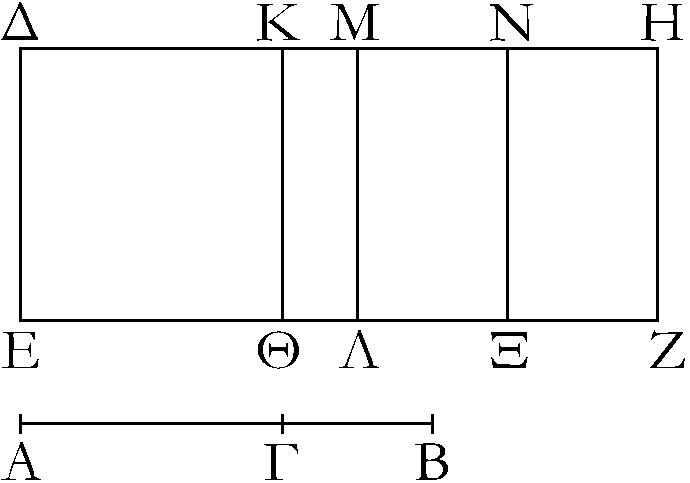
\includegraphics{Book10/fig060g.pdf}}

\gr{Κατεσκευάσθω τὰ α\kern -.7pt  ὐτὰ τοῖξ προδεδειγμένοιξ. καὶ ἐπεὶ μείζων
ἐστὶν ἡ ΑΒ διῃρημένη κατὰ τὸ Γ, αἱ ΑΓ, ΓΒ δυνάμει εἰσὶν ἀσύμμετροι ποιοῦσαι τὸ μὲν συγκείμενον ἐκ τῶν ἀπ> α\kern -.7pt  ὐτῶν
τετραγώνων <ρητόν, τὸ δὲ ὑπ> α\kern -.5pt  ὐτῶν μέσον. ἐπεὶ ο>ῦν <ρητόν
ἐστι τὸ συγκείμενον ἐκ τῶν ἀπὸ τῶν ΑΓ, ΓΒ, <ρητὸν >άρα ἐστὶ
τὸ ΔΛ; <ρητὴ >άρα καὶ ἡ ΔΜ καὶ σύμμετροξ τῆ| ΔΕ μ\kern -.3pt  ήκει.
πάλιν, ἐπεὶ μέσον ἐστὶ τὸ δὶξ ὑπὸ τῶν ΑΓ, ΓΒ, τουτέστι τὸ ΜΖ,
καὶ παρὰ <ρητήν ἐστι τὴν ΜΛ, <ρητὴ >άρα ἐστὶ καὶ ἡ ΜΗ καὶ
ἀσύμμετροξ  τῆ| ΔΕ μ\kern -.7pt  ήκει; ἀσύμμετροξ >άρα ἐστὶ καὶ ἡ ΔΜ
τῆ| ΜΗ μ\kern -.7pt  ήκει. αἱ ΔΜ, ΜΗ >άρα <ρηταί εἰσι δυνάμει μόνον σύμμετροι; ἐκ δύο >άρα ὀνομάτων ἐστὶν ἡ ΔΗ. δεικτέον
[δή], <ότι καὶ τετάρτη.}

\gr{Ὁμοίωξ δὴ δείχομεν τοῖξ πρότερον, <ότι μείζων ἐστὶν ἡ ΔΜ
τῆξ ΜΗ , καὶ <ότι τὸ ὑπὸ ΔΚΜ >ίσον ἐστὶ τῶ| ἀπὸ τῆξ
ΜΝ. ἐπεὶ ο>ῦν ἀσύμμετρόν ἐστι τὸ ἀπὸ τῆξ ΑΓ τῶ| ἀπὸ
τῆξ ΓΒ, ἀσύμμετρον >άρα ἐστὶ καὶ τὸ ΔΘ τῶ| ΚΛ; <ώστε
ἀσύμμετροξ καὶ ἡ ΔΚ τῆ| ΚΜ ἐστιν. ἒαν δὲ >ῶσι δύο εὐθεῖαι
>άνισοι, τῶ| δὲ τετάρτῳ μέρει τοῦ ἀπὸ τῆξ ἐλάσσονοξ >ίσον
παραλληλόγραμμον παρὰ τὴν μείζονα παραβληθῆ| ἐλλεῖπον ε>ίδει
τετραγώνῳ καὶ εἰξ ἀσύμμετρα α\kern -.7pt  ὐτὴν διαιρῆ|, ἡ μείζων τῆξ
ἐλάσσονοξ μεῖζον δυνήσεται τῶ| ἀπὸ ἀσύμμέτρου ἑαυτῆ|
μ\kern -.7pt  ήκει; ἡ ΔΜ >άρα τῆξ ΜΗ μεῖζον δύναται τῶ| ἀπὸ ἀσυμμέτρου
ἑαυτῆ|. καί εἰσιν αἱ ΔΜ, ΜΗ <ρηταὶ δυνάμει μόνον σύμμετροι,
καὶ ἡ ΔΜ σύμμετρόξ ἐστι τῆ| ἐκκειμένῃ <ρητῆ| τῆ| ΔΕ.}

\gr{Ἡ ΔΗ >άρα ἐκ δύο ὀνομάτων ἐστὶ τετάρτη; <όπερ >έδει δεῖχαι.}}

\ParallelRText{
\begin{center}
{\large Proposition 63}
\end{center}

The square on a major (straight-line) applied
to a rational (straight-line)  produces as breadth a fourth binomial (straight-line).$^\dag$

Let $AB$ be a major (straight-line) having been divided at $C$, such that
$AC$ is greater than $CB$, and (let) $DE$ (be)  a rational (straight-line). And
let the parallelogram $DF$, equal to the (square) on $AB$, be
applied to $DE$, producing $DG$ as breadth. I say that
$DG$ is a fourth binomial (straight-line).

% Removed epsf size command
\centerline{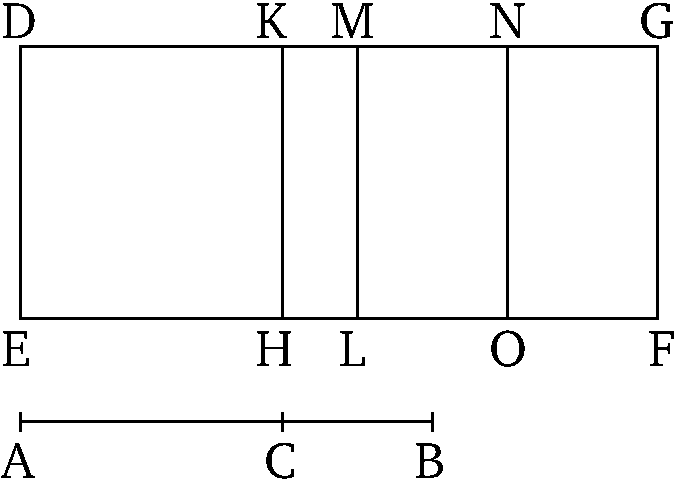
\includegraphics{Book10/fig060e.pdf}}

Let the same construction be made as that shown previously.
And since $AB$ is a major (straight-line), having been divided at $C$, $AC$ and
$CB$ are incommensurable in square, making the sum of the squares
on them rational, and the (rectangle contained) by them medial [Prop.~10.39]. Therefore, since the sum of the
(squares) on $AC$ and $CB$ is rational, $DL$ is thus rational.
Thus, $DM$ (is) also rational, and commensurable in length with $DE$ [Prop.~10.20]. Again, since twice the (rectangle
contained) by $AC$ and $CB$---that is to say, $MF$---is medial,
and is (applied to) the rational (straight-line) $ML$,  $MG$
is thus also rational, and incommensurable in length with $DE$ [Prop.~10.22]. $DM$ is thus also incommensurable
in length with $MG$ [Prop.~10.13]. $DM$
and $MG$ are thus rational (straight-lines which are) commensurable
in square only. Thus, $DG$ is a binomial (straight-line) [Prop.~10.36]. [So] we must show that (it is)
also a fourth (binomial straight-line).

So, similarly to the previous (propositions), we can show that $DM$ is
greater than $MG$, and that the (rectangle contained) by $DKM$
is equal to the (square) on $MN$. Therefore, since the (square) on $AC$
is incommensurable with the (square) on $CB$, $DH$ is also incommensurable
with $KL$. Hence, $DK$ is also incommensurable with $KM$
[Props.~6.1, 10.11].
And if there are two unequal straight-lines, and a parallelogram
equal to the fourth part of the (square) on the lesser, falling short
by a square figure, is applied to the greater, and divides it
into (parts which are) incommensurable (in length), then the square on
the greater will be larger than (the square on) the lesser by the
(square) on (some straight-line) incommensurable in length
with the greater [Prop.~10.18]. Thus,
the square on $DM$ is greater than (the square on) $MG$ by the
(square) on (some straight-line) incommensurable (in length) with ($DM$). And
$DM$ and $MG$ are rational (straight-lines which are) commensurable
in square only. And $DM$ is commensurable (in length)
with the (previously) laid down rational (straight-line) $DE$.

Thus, $DG$ is a fourth binomial (straight-line) [Def. 10.8]. (Which is) the very thing it was required
to show.}
\end{Parallel}
{\footnotesize\noindent$^\dag$ In other words, the square of a major is a
fourth binomial. See Prop.~10.57.\\}

%%%%
%10.64
%%%%
\pdfbookmark[1]{Proposition 10.64}{pdf10.64}
\begin{Parallel}{}{}
\ParallelLText{
\begin{center}
{\large \ggn{64}.}
\end{center}\vspace*{-7pt}

\gr{Τὸ ἀπὸ τῆξ <ρητὸν καὶ μέσον δυναμένηξ παρὰ <ρητὴν
παραβαλλόμενον πλάτοξ ποιεῖ τὴν ἐκ δύο ὀνομάτων
πέμπτην.}

\gr{>'Εστω <ρητὸν καὶ μέσον δυναμένη ἡ ΑΒ διῃρημένη εἰξ
τὰξ εὐθείαξ κατὰ τὸ Γ, <ώστε μείζονα ε>ῖναι τὴν ΑΓ,
καὶ ἐκκείσθω <ρητὴ ἡ ΔΕ, καὶ τῶ| ἀπὸ τῆξ ΑΒ >ίσον
παρὰ τὴν ΔΕ παραβεβλήσθω τὸ ΔΖ πλάτοξ ποιοῦν τὴν ΔΗ;
λέγω, <ότι ἡ ΔΗ ἐκ δύο ὀνομάτων ἐστὶ πέμπτη.}\\~\\

% Removed epsf size command
\centerline{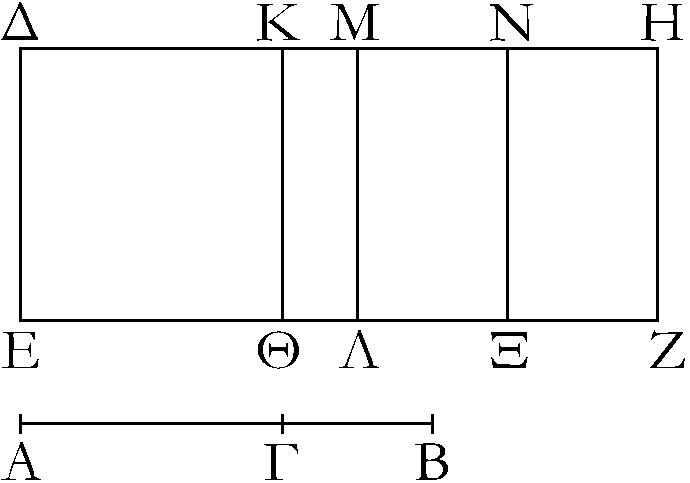
\includegraphics{Book10/fig060g.pdf}}

\gr{Κατεσκευάσθω τὰ α\kern -.7pt  ὐτα τοῖξ πρὸ τούτου. ἐπεὶ ο>ῦν
<ρητὸν καὶ μέσον δυναμένη ἐστὶν ἡ ΑΒ διῃρημένη
κατὰ τὸ Γ, αἱ ΑΓ, ΓΒ >άρα δυνάμει εἰσὶν ἀσύμμετροι
ποιοῦσαι τὸ μὲν συγκείμενον ἐκ τῶν ἀπ> α\kern -.7pt  ὐτῶν
τετραγώνων μέσον, τὸ δ> ὑπ> α\kern -.5pt  ὐτῶν <ρητόν. ἐπεὶ ο>ῦν
μέσον ἐστὶ τὸ συγκείμενον ἐκ τῶν ἀπὸ τῶν ΑΓ, ΓΒ,
μέσον >άρα ἐστὶ τὸ ΔΛ; <ώστε <ρητή ἐστιν ἡ ΔΜ καὶ
μ\kern -.3pt  ήκει ἀσύμμετροξ τῆ| ΔΕ. πάλιν, ἐπεὶ <ρητόν ἐστι τὸ δὶξ
ὑπὸ τῶν ΑΓΒ, τουτέστι τὸ ΜΖ, <ρητὴ >άρα ἡ ΜΗ 
καὶ σύμμετροξ τῆ| ΔΕ. ἀσύμμετροξ >άρα ἡ ΔΜ τῆ|
ΜΗ ; αἱ ΔΜ, ΜΗ >άρα <ρηταί εἰσι δυνάμει μόνον σύμμετροι;
ἐκ δύο >άρα ὀνομάτων ἐστὶν ἡ ΔΗ. λέγω δή, <ότι καὶ
πέμπτη.}

\gr{Ὁμοίωξ γὰρ διεθθήσεται, <ότι τὸ ὑπὸ τῶν ΔΚΜ >ίσον
ἐστὶ τῶ| ἀπὸ τῆξ ΜΝ, καὶ ἀσύμμετροξ ἡ ΔΚ τῆ| ΚΜ
μ\kern -.7pt  ήκει; ἡ ΔΜ >άρα τῆξ ΜΗ μεῖζον δύναται τῶ| ἀπὸ
ἀσυμμέτρου ἑαυτῆ|. καί εἰσιν αἱ ΔΜ, ΜΗ [<ρηταὶ] δυνάμει
μόνον σύμμετροι, καὶ ἡ ἐλάσσων ἡ ΜΗ σύμμετροξ τῆ|
ΔΕ μ\kern -.7pt  ήκει.}

\gr{Ἡ ΔΗ >άρα ἐκ δύο ὀνομάτων ἐστὶ πέμπτη; <όπερ
>έδει δεῖχαι.}}

\ParallelRText{
\begin{center}
{\large Proposition 64}
\end{center}

The square on the square-root of a rational
plus a medial (area) applied to a rational (straight-line) produces as breadth
a fifth binomial (straight-line).$^\dag$

Let $AB$ be the square-root of a rational plus a medial (area) having been divided
into its (component) straight-lines at $C$, such that $AC$ is greater. 
And let the rational (straight-line) $DE$ be laid down. And let the
(parallelogram) $DF$, equal to the (square) on $AB$, be applied
to $DE$, producing $DG$ as breadth. I say that $DG$ is a fifth
binomial straight-line.

% Removed epsf size command
\centerline{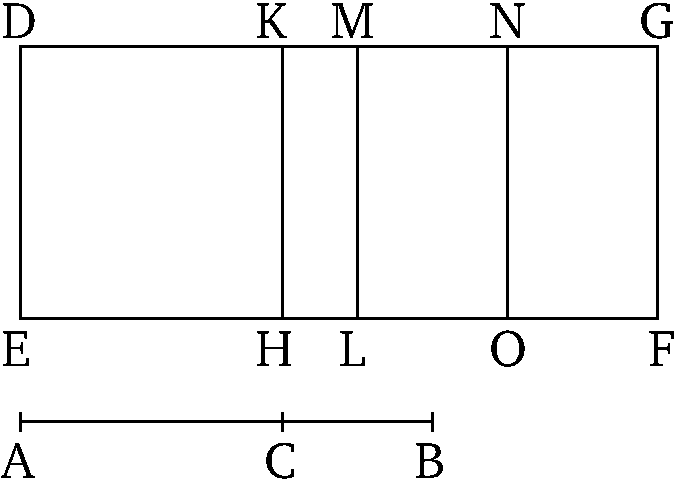
\includegraphics{Book10/fig060e.pdf}}

Let the same construction  be made as in the (propositions)
before this. Therefore, since $AB$ is the square-root of a
rational plus a medial (area), having been  divided at $C$, $AC$ and $CB$ are thus
incommensurable in square, making the sum of the squares on them
medial, and the (rectangle contained) by them rational [Prop.~10.40]. Therefore, since the
sum of the (squares) on $AC$ and $CB$ is medial, $DL$ is thus
medial. Hence, $DM$ is rational and incommensurable
in length with $DE$ [Prop.~10.22]. Again,
since twice the (rectangle contained) by $ACB$---that is to say,
$MF$---is rational, $MG$ (is) thus rational and commensurable
(in length) with $DE$ [Prop.~10.20]. 
$DM$ (is) thus incommensurable (in length) with $MG$ [Prop.~10.13]. Thus, $DM$ and $MG$
are rational (straight-lines which are) commensurable in square only. Thus,
$DG$ is a binomial (straight-line) [Prop.~10.36].
So, I say that (it is) also a fifth (binomial straight-line).

For, similarly (to the previous propositions), it can be shown that the
(rectangle contained) by $DKM$ is equal to the (square) on $MN$,
and $DK$ (is) incommensurable in length with $KM$. Thus, the
square on $DM$ is greater than (the square on) $MG$ by the (square)
on (some straight-line) incommensurable (in length) with ($DM$)
[Prop.~10.18]. And  $DM$ and $MG$
are [rational] (straight-lines which are) commensurable in square only,
and the lesser $MG$ is commensurable in length with $DE$.

Thus, $DG$ is a fifth binomial (straight-line) [Def.~10.9]. (Which is) the very thing it was required to show.}
\end{Parallel}
{\footnotesize\noindent$^\dag$ In other words, the square of the square-root of a rational plus medial  is a
fifth binomial. See Prop.~10.58.}

%%%%
%10.65
%%%%
\pdfbookmark[1]{Proposition 10.65}{pdf10.65}
\begin{Parallel}{}{}
\ParallelLText{
\begin{center}
{\large \ggn{65}.}
\end{center}\vspace*{-7pt}

\gr{Τὸ ἀπὸ τῆξ δύο μέσα δυναμένηξ παρὰ <ρητὴν παραβαλλόμενον
πλάτοξ ποιεῖ τὴν ἐκ δύο ὀνομάτων <έκτην.}

\gr{>'Εστω δύο μέσα δυναμένη ἡ ΑΒ διῃρημένη κατὰ τὸ Γ, <ρητὴ
δὲ >έστω ἡ ΔΕ, καὶ παρὰ τὴν ΔΕ τῶ| ἀπὸ τῆξ ΑΒ >ίσον παραβεβλήσθω τὸ ΔΖ πλάτοξ ποιοῦν τὴν ΔΗ; λέγω, <ότι ἡ ΔΗ
ἐκ δύο ὀνομάτων ἐστὶν <έκτη.}\\~\\

% Removed epsf size command
\centerline{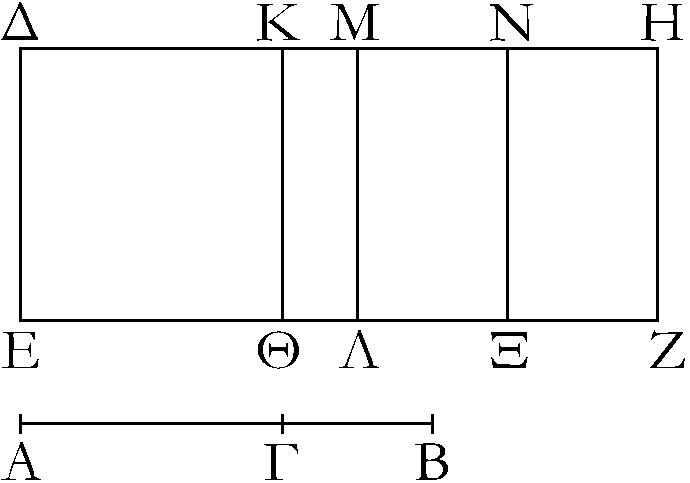
\includegraphics{Book10/fig060g.pdf}}

\gr{Κατεσκευάσθω γὰρ τὰ α\kern -.7pt  ὐτὰ τοῖξ πρότερον. καὶ ἐπεὶ ἡ ΑΒ
δύο μέσα δυναμένη ἐστὶ διῃρημένη κατὰ τὸ Γ, αἱ ΑΓ, ΓΒ
>άρα δυνάμει εἰσὶν ἀσύμμετροι ποιοῦσαι τό τε συγκείμενον
ἐκ τῶν ἀπ> α\kern -.7pt  ὐτῶν τετραγώνων μέσον καὶ τὸ ὑπ> α\kern -.5pt  ὐτῶν
μέσον καὶ >έτι ἀσύμμετρον τὸ ἐκ τῶν ἀπ> α\kern -.3pt  ὐτῶν
τετραγώνων συγκείμενον τῶ| ὑπ> α\kern -.7pt  ὐτῶν; <ώστε κατὰ τὰ
προδεδειγμένα μέσον ἐστὶν ἑκάτερον τῶν ΔΛ, ΜΖ. καὶ παρὰ
<ρητὴν τὴν ΔΕ παράκειται; <ρητὴ >άρα ἐστὶν ἑκατέρα τῶν
ΔΜ, ΜΗ καὶ ἀσύμμετροξ τῆ| ΔΕ μ\kern -.7pt  ήκει. καὶ ἐπεὶ ἀσύμμετρόν
ἐστι τὸ συγκείμενον ἐκ τῶν ἀπὸ τῶν ΑΓ, ΓΒ τῶ| δὶξ
ὑπὸ τῶν ΑΓ, ΓΒ, ἀσύμμετρον >άρα ἐστὶ τὸ ΔΛ τῶ| ΜΖ. ἀσύμμετροξ >άρα καὶ ἡ ΔΜ τῆ| ΜΗ ; αἱ ΔΜ, ΜΗ  >άρα <ρηταί
εἰσι δυνάμει μόνον σύμμετροι; ἐκ δύο >άρα ὀνομάτων ἐστὶν
ἡ ΔΗ. λέγω δή, <ότι καὶ <έκτη.}

\gr{Ὁμοίωξ δὴ πάλιν δεῖχομεν, <ότι τὸ ὑπὸ τῶν ΔΚΜ >ίσον
ἐστὶ τῶ| ἀπὸ τῆξ ΜΝ, καὶ <ότι ἡ ΔΚ τῆ| ΚΜ μ\kern -.7pt  ήκει ἐστὶν
ἀσύμμετροξ; καὶ διὰ τὰ α\kern -.7pt  ὐτὰ δὴ ἡ ΔΜ τῆξ ΜΗ μεῖζον
δύναται τῶ| ἀπὸ ἀσυμμέτρου ἑαυτῆ| μ\kern -.5pt  ήκει. καὶ
οὐδετέρα τῶν ΔΜ, ΜΗ σύμμετρόξ ἐστι τῆ| ἐκκειμένῃ <ρητῆ|
τῆ| ΔΕ μ\kern -.3pt  ήκει.}

\gr{Ἡ ΔΗ >άρα ἐκ δύο ὀνομάτων ἐστὶν <έκτη; <όπερ
>έδει δεῖχαι.}}

\ParallelRText{
\begin{center}
{\large Proposition 65}
\end{center}

The square on the square-root of (the sum of) two medial
(areas) applied to a rational (straight-line) produces as breadth  a sixth binomial (straight-line).$^\dag$

Let $AB$ be the square-root of (the sum of) two medial (areas), having been divided
at $C$. And let $DE$ be a  rational (straight-line). And let the (parallelogram) $DF$, equal to the (square) on $AB$, be applied to $DE$, producing $DG$
as breadth. I say that $DG$ is a sixth binomial (straight-line).

% Removed epsf size command
\centerline{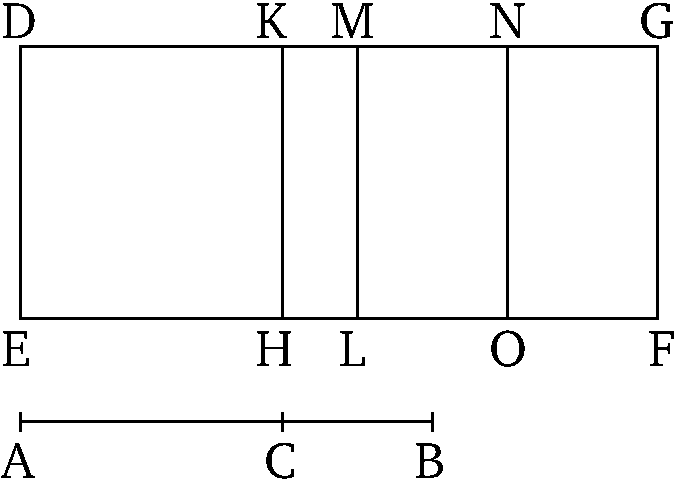
\includegraphics{Book10/fig060e.pdf}}

For  let the same construction  be made  as in the previous (propositions). And since $AB$ is the square-root of (the sum of) two medial
(areas), having been divided at $C$, $AC$ and $CB$ are thus incommensurable
in square, making the sum of the squares on them medial, and the (rectangle
contained) by them medial, and, moreover, the sum of the squares on them
incommensurable with the (rectangle contained) by them [Prop.~10.41]. Hence, according to
what has been previously  demonstrated, $DL$ and $MF$ are each medial.
And they are applied to the rational (straight-line) $DE$. Thus, $DM$ and
$MG$ are each rational, and incommensurable in length with $DE$ [Prop.~10.22]. And since the sum of the (squares)
on $AC$ and $CB$ is incommensurable with twice the (rectangle contained)
by $AC$ and $CB$, $DL$ is thus incommensurable with $MF$. Thus,
$DM$ (is) also incommensurable (in length) with $MG$
[Props.~6.1, 10.11]. 
$DM$ and $MG$ are thus rational (straight-lines which are) commensurable
in square only. Thus, $DG$ is a binomial (straight-line) [Prop.~10.36]. So, I say that (it is) also a sixth
(binomial straight-line).

So, similarly (to the previous propositions), we can again show that the (rectangle contained) by $DKM$ is equal to the (square) on $MN$, and that
$DK$ is incommensurable in length with $KM$. And so, for the same (reasons), the square on $DM$ is greater than (the square on) $MG$ by the
(square) on (some straight-line) incommensurable in length with ($DM$) [Prop.~10.18]. And neither of $DM$ and $MG$
is commensurable in length with the (previously) laid down rational (straight-line) $DE$.

Thus, $DG$ is a sixth binomial (straight-line) [Def. 10.10]. (Which is) the very thing it
was required to show.}
\end{Parallel}
{\footnotesize\noindent $^\dag$ In other words, the square of the square-root of  two  medials  is a
sixth binomial. See Prop.~10.59.\\}

%%%%
%10.66
%%%%
\pdfbookmark[1]{Proposition 10.66}{pdf10.66}
\begin{Parallel}{}{}
\ParallelLText{
\begin{center}
{\large \ggn{66}.}
\end{center}\vspace*{-7pt}

\gr{Ἡ τῆ| ἐκ δύο ὀνομάτων μ\kern -.7pt  ήκει σύμμετροξ καὶ α\kern -.7pt  ὐτὴ ἐκ δύο
ὀνομάτων ἐστὶ καὶ τῆ| τάχει ἡ α\kern -.5pt  ὐτή.}

\gr{>'Εστω ἐκ δύο ὀνομάτων ἡ ΑΒ, καὶ τῆ| ΑΒ μ\kern -.7pt  ήκει σύμμετροξ
>έστω ἡ ΓΔ; λέγω, <ότι ἡ ΓΔ ἐκ δύο ὀνομάτων ἐστὶ καὶ τῆ|
τάχει ἡ α\kern -.7pt  ὐτὴ τῆ| ΑΒ.}

% Removed epsf size command
\centerline{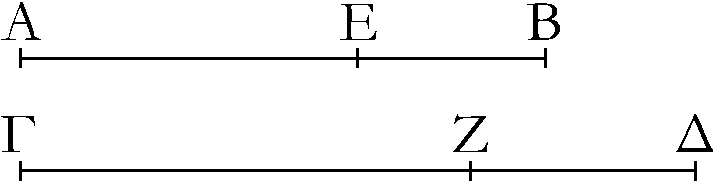
\includegraphics{Book10/fig066g.pdf}}

\gr{Ἐπεὶ γὰρ ἐκ δύο ὀνομάτων ἐστὶν ἡ ΑΒ, διῃρήσθω εἰξ τὰ
ὀνόματα κατὰ τὸ Ε, καὶ >έστω μεῖζον >όνομα τὸ ΑΕ; αἱ ΑΕ, ΕΒ >άρα
<ρηταί εἰσι δυνάμει μόνον σύμμετροι. γεγονέτω ὡξ ἡ ΑΒ πρὸξ
τὴν ΓΔ, ο<ύτωξ ἡ ΑΕ πρὸξ τὴν ΓΖ; καὶ λοιπὴ >άρα ἡ ΕΒ πρὸξ
λοιπὴν τὴν ΖΔ ἐστιν, ὡξ ἡ ΑΒ πρὸξ τὴν ΓΔ. σύμμετροξ δὲ ἡ ΑΒ τῆ| ΓΔ μ\kern -.7pt  ήκει; σύμμετροξ >άρα ἐστὶ καὶ ἡ μὲν ΑΕ τῆ| ΓΖ, ἡ
δὲ ΕΒ τῆ| ΖΔ. καί εἰσι <ρηταὶ αἱ ΑΕ, ΕΒ; <ρηταὶ >άρα εἰσὶ καὶ αἱ
ΓΖ, ΖΔ. καὶ  ἐστιν ὡξ ἡ ΑΕ πρὸξ ΓΖ, ἡ ΕΒ πρὸξ ΖΔ. ἐναλλὰχ
>άρα ἐστὶν ὡξ ἡ ΑΕ πρὸξ ΕΒ, ἡ ΓΖ πρὸξ ΖΔ.
αἱ δὲ
ΑΕ, ΕΒ δυνάμει μόνον [εἰσὶ] σύμμετροι; καὶ αἱ ΓΖ, ΖΔ >άρα
δυνάμει μόνον  εἰσὶ σύμμετροι.
καί εἰσι <ρηταί;
ἐκ δύο >άρα ὀνομάτων ἐστὶν ἡ ΓΔ. λέγω δή, <ότι τῆ| τάχει
ἐστὶν ἡ α\kern -.7pt  ὐτὴ τῆ| ΑΒ.}

\gr{Ἡ γὰρ ΑΕ τῆξ ΕΒ μεῖζον δύναται >ήτοι τῶ| ἀπὸ συμμέτρου
ἑαυτῆ| >ὴ τῶ| ἀπὸ ἀσυμμέτρου. εἰ μὲν ο>ῦν ἡ ΑΕ τῆξ
ΕΒ μεῖζον δύναται τῶ| ἀπὸ συμμέτρου ἑαυτῆ|, καὶ ἡ ΓΖ τῆξ
ΖΔ μεῖζον δυνήσεται τῶ| ἀπὸ συμμέτρου ἑαυτῆ|. καὶ εἰ μὲν
σύμμετρόξ ἐστιν ἡ ΑΕ τῆ| ἐκκειμένῃ <ρητῆ|, καὶ ἡ ΓΖ σύμμετροξ
α\kern -.7pt  ὐτῆ| >έσται, καὶ διὰ τοῦτο ἑκατέρα τῶν ΑΒ, ΓΔ ἐκ δύο ὀνομάτων
ἐστὶ πρώτη, τουτέστι τῆ| τάχει ἡ α\kern -.7pt  ὐτή. εἰ δὲ ἡ ΕΒ σύμμετρόξ
ἐστι τῆ| ἐκκειμένῃ <ρητῆ|, καὶ ἡ ΖΔ σύμμετρόξ ἐστιν α\kern -.5pt  ὐτῆ|, καὶ
διὰ τοῦτο πάλιν τῆ| τάχει ἡ α\kern -.3pt  ὐτὴ >έσται τῆ| ΑΒ; ἑκατέρα γὰρ
α\kern -.7pt  ὐτῶν >έσται ἐκ δύο ὀνομάτων δευτέρα. εἰ δὲ οὐδετέρα
τῶν ΑΕ, ΕΒ σύμμετρόξ ἐστι τῆ| ἐκκειμένῃ <ρητῆ|, οὐδετέρα
τῶν ΓΖ, ΖΔ σύμμετροξ α\kern -.7pt  ὐτῆ| >έσται, καί ἐστιν ἑκατέρα τρίτη. εἰ δὲ
ἡ ΑΕ τῆξ ΕΒ μεῖζον δύναται τῶ| ἀπὸ ἀσυμμέτρου ἑαυτῆ|,
καὶ ἡ ΓΖ τὴξ ΖΔ μεῖζον δύναται τῶ| ἀπὸ ἀσυμμέτρου
ἑαυτῆ|. καὶ εἰ μὲν ἡ ΑΕ σύμμετρόξ ἐστι τῆ| ἐκκειμένῃ <ρητῃ,
καὶ ἡ ΓΖ σύμμετρόξ ἐστιν α\kern -.7pt  ὐτῆ|, καὶ ἐστιν ἑκατέρα τετάρτη.
εἰ δὲ ἡ ΕΒ, καὶ ἡ ΖΔ, καὶ >έσται ἑκατέρα πέμπτη. εἰ δὲ οὐδετέρα
τῶν ΑΕ, ΕΒ, καὶ τῶν ΓΖ, ΖΔ οὐδετέρα σύμμετρόξ ἐστι τῆ| ἐκκειμένῃ <ρητῆ|, καὶ >έσται ἑκατέρα <έκτη.}

\gr{<'Ωστε ἡ τῆ| ἐκ δύο ὀνομάτων μ\kern -.7pt  ήκει σύμμετροξ ἐκ δύο
ὀνομάτων ἐστὶ καὶ τῆ| τάχει ἡ α\kern -.7pt  ὐτή; <όπερ >έδει δεῖχαι.
}}

\ParallelRText{
\begin{center}
{\large Proposition 66}
\end{center}

A (straight-line) commensurable in length with
a binomial (straight-line) is itself also binomial, and the same in order.

Let $AB$ be a binomial (straight-line), and let $CD$ be commensurable
in length with $AB$. I say that $CD$ is a binomial (straight-line),
and (is)  the same in order as $AB$.

% Removed epsf size command
\centerline{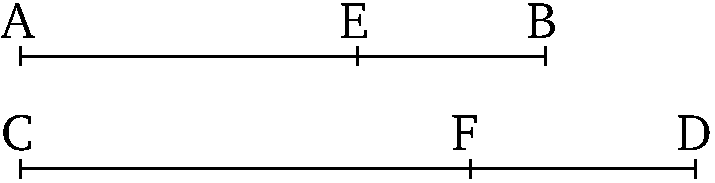
\includegraphics{Book10/fig066e.pdf}}

For since $AB$ is a binomial (straight-line), let it be divided into
its (component) terms at $E$, and let $AE$ be the greater term. $AE$ and
$EB$ are thus rational (straight-lines which are) commensurable in square only [Prop.~10.36]. Let it be contrived
that as $AB$ (is) to $CD$, so $AE$ (is) to $CF$ [Prop.~6.12]. Thus, the remainder $EB$ is also
to the remainder $FD$, as $AB$ (is) to $CD$ [Props.~6.16, 5.19~corr.]. 
And $AB$ (is) commensurable in length with $CD$. Thus, $AE$ is also
commensurable (in length) with $CF$, and $EB$ with $FD$ [Prop.~10.11]. And $AE$ and $EB$ are rational.
Thus, $CF$ and $FD$ are also rational. And  as $AE$
is to $CF$, (so) $EB$ (is) to $FD$ [Prop.~5.11]. 
Thus, alternately, as $AE$ is to $EB$, (so) $CF$ (is) to $FD$ [Prop.~5.16]. And $AE$ and $EB$ [are]
commensurable in square only. Thus, $CF$ and $FD$ are also
commensurable in square only [Prop.~10.11]. 
And they are rational. $CD$ is thus a binomial (straight-line) [Prop.~10.36]. So, I say that it is the same in order as $AB$.

For the square on $AE$ is  greater than (the square on) $EB$ by the
(square) on (some straight-line) either commensurable or incommensurable
(in length) with ($AE$).  Therefore, if the square on $AE$ is greater than (the square on)
$EB$ by the (square) on (some straight-line) commensurable (in length)
with ($AE$) then the square on $CF$ will also be greater than (the square on)
$FD$ by the (square) on (some straight-line) commensurable (in length)
with ($CF$) [Prop.~10.14]. And if $AE$
is commensurable (in length) with (some previously) laid down rational (straight-line) then $CF$ will also be commensurable (in length) with it [Prop.~10.12]. And, on account of this,
$AB$ and $CD$ are each first binomial (straight-lines) [Def.~10.5]---that is to say, the same  in order.
And if $EB$ is commensurable (in length) with the (previously) laid down
rational (straight-line) then $FD$ is also  commensurable (in length) with it [Prop.~10.12], and, again, on account of this,
($CD$) will be  the same in order as $AB$. For each of them will be second
binomial (straight-lines) [Def.~10.6]. And if neither
of $AE$ and $EB$ is commensurable (in length) with the (previously) laid down
rational (straight-line) then neither of $CF$ and $FD$ will be commensurable (in length)
with it [Prop.~10.13], and each (of $AB$ and $CD$) is a third (binomial straight-line) [Def.~10.7]. And if the square on $AE$
is greater than (the square on) $EB$ by the (square) on (some straight-line)
incommensurable (in length) with ($AE$) then the square on $CF$
is also greater than (the square on) $FD$ by the (square) on (some straight-line) incommensurable (in length) with ($CF$) [Prop.~10.14]. And if $AE$ is commensurable
(in length) with the (previously) laid down rational (straight-line) then $CF$ is also
commensurable (in  length) with it [Prop.~10.12], 
and each (of $AB$ and $CD$) is a fourth (binomial straight-line)
[Def.~10.8]. And
if $EB$ (is commensurable in length with the previously laid down rational
straight-line) then $FD$ (is) also (commensurable in length with it), and
each (of $AB$ and $CD$) will be a fifth (binomial straight-line) [Def.~10.9]. And if neither of $AE$ and  $EB$
(is commensurable in length with the previously laid down rational
straight-line) then also neither of $CF$ and $FD$ is   commensurable (in length) with the laid down rational (straight-line), and
each (of $AB$ and $CD$) will be a sixth (binomial straight-line) [Def.~10.10].

Hence, a (straight-line) commensurable in length with a binomial (straight-line) is a binomial (straight-line), and the same in order. (Which is) the
very thing it was required to show.}
\end{Parallel}

%%%%
%10.67
%%%%
\pdfbookmark[1]{Proposition 10.67}{pdf10.67}
\begin{Parallel}{}{}
\ParallelLText{
\begin{center}
{\large\ggn{67}.}
\end{center}\vspace*{-7pt}

\gr{Ἡ τῆ| ἐκ δύο μέσων μ\kern -.7pt  ήκει σύμμετροξ καὶ α\kern -.7pt  ὐτὴ ἐκ δύο μέσων
ἐστὶ καὶ τῆ| τάχει ἡ α\kern -.5pt  ὐτή.}

% Removed epsf size command
\centerline{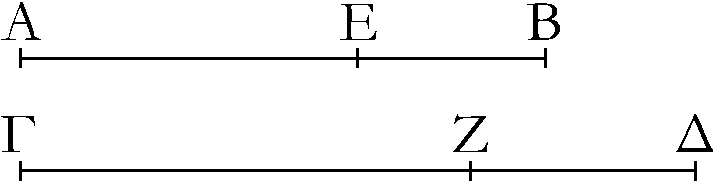
\includegraphics{Book10/fig066g.pdf}}

\gr{>'Εστω ἐκ δύο μέσων ἡ ΑΒ, καὶ τῆ| ΑΒ σύμμετροξ >έστω μ\kern -.7pt  ήκει
ἡ ΓΔ; λέγω, <ότι ἡ ΓΔ ἐκ δύο μέσων ἐστὶ καὶ τῆ| τάχει
ἡ α\kern -.7pt  ὐτὴ τῆ| ΑΒ.}

\gr{Ἐπεὶ γὰρ ἐκ δύο μέσων ἐστὶν ἡ ΑΒ, διῃρήσθω εἰξ τὰξ
μέσαξ κατὰ τὸ Ε; αἱ ΑΕ, ΕΒ >άρα μέσαι εἰσὶ δυνάμει μόνον
σύμμετροι. καὶ γεγονέτω ὡξ ἡ ΑΒ πρὸξ ΓΔ, ἡ ΑΕ πρὸξ ΓΖ;
καὶ λοιπὴ >άρα ἡ ΕΒ πρὸξ λοιπὴν τὴν ΖΔ ἐστιν, ὡξ ἡ ΑΒ πρὸξ ΓΔ. σύμμετροξ δὲ ἡ ΑΒ τῆ| ΓΔ μ\kern -.7pt  ήκει; σύμμετροξ >άρα καὶ ἑκατέρα τῶν
ΑΕ, ΕΒ ἑκατέρᾳ τῶν ΓΖ, ΖΔ. μέσαι δὲ αἱ ΑΕ, ΕΒ; μέσαι >άρα καὶ αἱ
ΓΖ, ΖΔ. καὶ ἐπεί ἐστιν ὡξ ἡ ΑΕ πρὸξ ΕΒ, ἡ ΓΖ πρὸξ ΖΔ, αἱ 
δὲ ΑΕ, ΕΒ δυνάμει μόνον σύμμετροί εἰσιν, καὶ αἱ ΓΖ, ΖΔ [>άρα]
δυνάμει μόνον σύμμετροί εἰσιν, ἐδείθθησαν δὲ καὶ μέσαι; ἡ
ΓΔ >άρα ἐκ δύο μέσων ἐστίν. λέγω δή, <ότι καὶ τῆ| τάχει ἡ
α\kern -.7pt  ὐτή ἐστι τῆ| ΑΒ.}

\gr{Ἐπεὶ γάρ ἐστιν ὡξ ἡ ΑΕ πρὸξ ΕΒ, ἡ ΓΖ πρὸξ ΖΔ, καὶ ὡξ
>άρα τὸ ἀπὸ τῆξ ΑΕ πρὸξ τὸ ὑπὸ τῶν ΑΕΒ, ο<ύτωξ
τὸ ἀπὸ τῆξ ΓΖ πρὸξ τὸ ὑπὸ τῶν ΓΖΔ; ἐναλλὰχ ὡξ τὸ
ἀπὸ τῆξ ΑΕ πρὸξ τὸ ἀπὸ τῆξ ΓΖ, ο<ύτωξ τὸ ὑπὸ τῶν ΑΕΒ
πρὸξ τὸ ὑπὸ τῶν ΓΖΔ. σύμμετρον δὲ τὸ ἀπὸ τῆξ
ΑΕ τῶ| ἀπὸ τῆξ ΓΖ; σύμμετρον
>άρα καὶ τὸ ὑπὸ τῶν ΑΕΒ τῶ| ὑπὸ τῶν ΓΖΔ. ε>ίτε ο>ῦν <ρητόν
ἐστι τὸ ὑπὸ τῶν ΑΕΒ, καὶ τὸ ὑπὸ τῶν ΓΖΔ <ρητόν ἐστιν
[καὶ διὰ τοῦτό ἐστιν ἐκ δύο μέσων πρώτη]. ε>ίτε μέσον, μέσον,
καί ἐστιν ἑκατέρα δευτέρα.}

\gr{Καὶ διὰ τοῦτο >έσται ἡ ΓΔ τῆ| ΑΒ τῆ| τάχει ἡ
α\kern -.7pt  ὐτή; <όπερ >έδει δεῖχαι.}}

\ParallelRText{
\begin{center}
{\large Proposition 67}
\end{center}

A (straight-line) commensurable
in length with a bimedial (straight-line) is  itself also bimedial, and
 the same in order.

% Removed epsf size command
\centerline{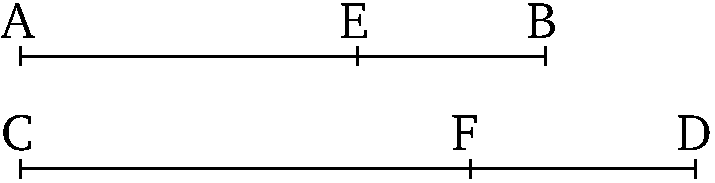
\includegraphics{Book10/fig066e.pdf}}
 
Let $AB$ be a bimedial (straight-line), and let $CD$ be commensurable
in length with $AB$. I say that $CD$ is bimedial, and the same in order as
$AB$.

For since $AB$ is a bimedial (straight-line), let it be divided into its
(component) medial (straight-lines) at $E$. Thus, $AE$ and $EB$
are medial (straight-lines which are) commensurable in square only [Props.~10.37, 10.38]. And
let it be contrived that as $AB$ (is) to $CD$, (so) $AE$ (is)
to $CF$ [Prop.~6.12]. And thus as the remainder $EB$ is to the remainder $FD$, so $AB$ (is) to $CD$ [Props.~5.19~corr., 6.16].
And $AB$ (is) commensurable in length with $CD$. Thus, $AE$
and $EB$ are also commensurable (in length) with $CF$ and $FD$, respectively [Prop.~10.11]. And 
$AE$ and $EB$ (are) medial. Thus, $CF$ and $FD$ (are) also
medial [Prop.~10.23]. And since as $AE$
is to $EB$, (so) $CF$ (is) to $FD$, and $AE$ and $EB$ are commensurable
in square only, $CF$ and $FD$ are [thus] also commensurable in square only
[Prop.~10.11]. And they were also shown (to be)
medial. Thus, $CD$ is a bimedial (straight-line). So, I say that it is also the same in order as $AB$.

For since as $AE$ is to $EB$, (so) $CF$ (is) to $FD$, thus also as the
(square) on $AE$ (is) to the (rectangle contained) by $AEB$, so the (square)
on $CF$ (is) to the (rectangle contained) by $CFD$ [Prop.~10.21~lem.]. Alternately, as the (square)
on $AE$ (is) to the (square) on $CF$, so the (rectangle
contained) by $AEB$ (is) to the (rectangle contained) by $CFD$ [Prop.~5.16]. And the (square) on $AE$
(is) commensurable with the (square) on $CF$. Thus, the (rectangle
contained) by $AEB$ (is) also commensurable with the (rectangle contained)
by $CFD$ [Prop.~10.11]. Therefore,  either the
(rectangle contained) by $AEB$ is rational, and  the (rectangle contained) by
$CFD$ is rational [and, on account of this, ($AE$ and $CD$) are first
bimedial (straight-lines)], or (the rectangle contained by $AEB$ is) medial,
and (the rectangle contained by $CFD$ is) medial, and ($AB$ and
$CD$) are each second (bimedial straight-lines) [Props.~10.23, 10.37, 10.38].

And, on account of this, $CD$ will be  the same in order as $AB$.
(Which is) the very thing it was required to show.}
\end{Parallel}

%%%%
%10.68
%%%%
\pdfbookmark[1]{Proposition 10.68}{pdf10.68}
\begin{Parallel}{}{}
\ParallelLText{
\begin{center}
{\large\ggn{68}.}
\end{center}\vspace*{-7pt}

\gr{Ἡ τῆ| μείζονι σύμμετροξ καὶ α\kern -.7pt  ὐτὴ μείζων ἐστίν.}\\

% Removed epsf size command
\centerline{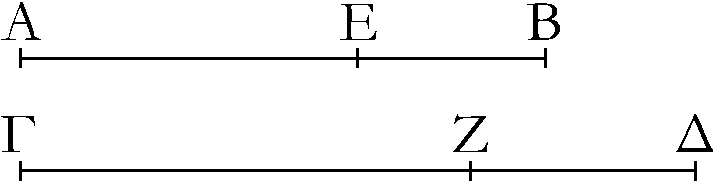
\includegraphics{Book10/fig066g.pdf}}

\gr{>'Εστω μείζων ἡ ΑΒ, καὶ τῆ| ΑΒ σύμμετροξ >έστω ἡ ΓΔ; λέγω,
<ότι ἡ ΓΔ μείζων ἐστίν.}

\gr{Διῃρήσθω ἡ ΑΒ κατὰ τὸ Ε; αἱ ΑΕ, ΕΒ >άρα δυνάμει εἰσὶν ἀσύμμετροι ποιοῦσαι τὸ μὲν συγκείμενον ἐκ τῶν ἀπ> α\kern -.7pt  ὐτῶν
τετραγώνων <ρητόν, τὸ δ> ὑπ> α\kern -.7pt  ὐτῶν μέσον; καὶ γεγονέτω
τὰ α\kern -.5pt  ὐτὰ τοῖξ πρότερον. καὶ ἐπεί ἐστιν ὡξ ἡ ΑΒ πρὸξ τὴν
ΓΔ, ο<ύτωξ <ή τε ΑΕ πρὸξ τὴν ΓΖ καὶ ἡ ΕΒ πρὸξ τὴν ΖΔ, καὶ ὡξ >άρα ἡ ΑΕ πρὸξ τὴν ΓΖ, ο<ύτωξ ἡ ΕΒ πρὸξ τὴν ΖΔ. σύμμετροξ
δὲ ἡ ΑΒ τῆ| ΓΔ; σύμμετροξ >άρα καὶ ἑκατέρα τῶν ΑΕ, ΕΒ ἑκατέρᾳ
τῶν ΓΖ, ΖΔ. καὶ ἐπεί ἐστιν ὡξ ἡ ΑΕ πρὸξ τὴν ΓΖ, ο<ύτωξ
ἡ ΕΒ πρὸξ τὴν ΖΔ,  καὶ
ἐναλλὰχ ὡξ ἡ ΑΕ πρὸξ ΕΒ, ο<ύτωξ ἡ ΓΖ πρὸξ ΖΔ, καὶ
συνθέντι >άρα ἑστὶν ὡξ ἡ ΑΒ πρὸξ τὴν ΒΕ, ο<ύτωξ  ἡ ΓΔ πρὸξ
τὴν ΔΖ; καὶ ὡξ >άρα τὸ ἀπὸ τῆξ ΑΒ πρὸξ τὸ ἀπὸ τῆξ ΒΕ, ο<ύτωξ
τὸ ἀπὸ τῆξ ΓΔ πρὸξ τὸ ἀπὸ τῆξ ΔΖ. ὁμοίωξ δὴ δείχομεν,
<ότι καὶ ὡξ τὸ ἀπὸ τῆξ ΑΒ πρὸξ τὸ ἀπὸ τῆξ ΑΕ, ο<ύτωξ
τὸ ἀπὸ τῆξ ΓΔ πρὸξ τὸ ἀπὸ τῆξ ΓΖ. καὶ ὡξ >άρα τὸ ἀπὸ
τῆξ ΑΒ πρὸξ τὰ ἀπὸ τῶν ΑΕ, ΕΒ, ο<ύτωξ τὸ ἀπὸ τῆξ ΓΔ
πρὸξ τὰ ἀπὸ τῶν ΓΖ, ΖΔ; καὶ ἐναλλὰχ >άρα ἐστὶν ὡξ τὸ
ἀπὸ τῆξ ΑΒ πρὸξ τὸ ἀπὸ τῆξ ΓΔ, ο<ύτωξ τὰ ἀπὸ τῶν
ΑΕ, ΕΒ πρὸξ τὰ ἀπὸ τῶν ΓΖ, ΖΔ. σύμμετρον δὲ τὸ ἀπὸ
τῆξ ΑΒ τῶ| ἀπὸ τῆξ ΓΔ; σύμμετρα >άρα καὶ τὰ ἀπὸ τῶν ΑΕ, ΕΒ
τοῖξ ἀπὸ τῶν ΓΖ, ΖΔ. καί ἐστι τὰ ἀπὸ τῶν ΑΕ, ΕΒ <άμα
<ρητόν, καὶ τὰ ἀπὸ τῶν ΓΖ, ΖΔ <άμα <ρητόν ἐστιν. ὁμοίωξ
δὲ καὶ τὸ δὶξ ὑπὸ τῶν ΑΕ, ΕΒ σύμμετρόν ἐστι τῶ| δὶξ
ὑπὸ τῶν
ΓΖ, ΖΔ. καί ἐστι μέσον τὸ δὶξ ὑπὸ τῶν ΑΕ, ΕΒ;
μέσον >άρα καὶ τὸ δὶξ ὑπὸ τῶν ΓΖ, ΖΔ. αἱ ΓΖ, ΖΔ
>άρα δυνάμει ἀσύμμετροί
εἰσι ποιοῦσαι τὸ μὲν συγκείμενον ἐκ τῶν ἀπ> α\kern -.3pt  ὐτῶν
τετραγώνων <άμα <ρητόν, τὸ δὲ δὶξ ὑπ> α\kern -.7pt  ὐτῶν μέσον;
<όλη >άρα ἡ ΓΔ >άλογόξ ἐστιν ἡ καλουμένη μείζων.}

\gr{Ἡ >άρα τῆ| μείζονι σύμμετροξ μείζων ἐστίν; <όπερ
>έδει δεῖχαι.}}

\ParallelRText{
\begin{center}
{\large Proposition 68}
\end{center}

A (straight-line) commensurable (in length)
with a major (straight-line) is  itself also major.

% Removed epsf size command
\centerline{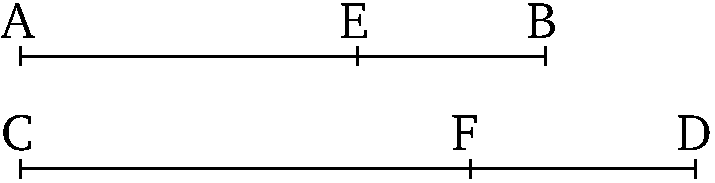
\includegraphics{Book10/fig066e.pdf}}

Let $AB$ be a major (straight-line), and let $CD$ be commensurable (in
length) with $AB$. I say that $CD$ is a major (straight-line).

Let $AB$ be divided (into its component terms) at $E$.
$AE$ and $EB$ are thus incommensurable in square, making the sum
of the squares on them rational, and the (rectangle contained) by them
medial [Prop.~10.39]. And let (the) same (things) be contrived as in the previous (propositions). And since
as $AB$ is to $CD$, so $AE$ (is) to $CF$ and $EB$ to $FD$, 
thus also as $AE$ (is) to $CF$, so $EB$ (is) to $FD$ [Prop.~5.11]. And $AB$ (is) commensurable
(in length) with $CD$. Thus, $AE$ and $EB$ (are) also commensurable
(in length) with $CF$ and $FD$, respectively [Prop.~10.11].  And since as $AE$ is to $CF$, so
$EB$ (is) to $FD$, also, alternately, as $AE$ (is) to $EB$, so
$CF$ (is) to $FD$ [Prop.~5.16], and thus, via composition, as $AB$ is to $BE$, so $CD$ (is) to $DF$ [Prop.~5.18]. And thus as the (square) on $AB$
(is) to the (square) on $BE$, so the (square) on $CD$ (is) to the (square)
on $DF$ [Prop.~6.20]. So, similarly, we can also show that as the (square) on $AB$ (is) to the (square) on $AE$, so the
(square) on $CD$ (is) to the (square) on $CF$. And thus as the (square)
on $AB$ (is) to (the sum of) the (squares) on $AE$ and $EB$, so
the (square) on $CD$ (is) to (the sum of) the (squares) on $CF$ and $FD$.
And thus, alternately, as the (square) on $AB$ is to the (square) on $CD$,
so (the sum of) the (squares) on $AE$ and $EB$ (is) to (the sum of)
the (squares) on $CF$ and $FD$ [Prop.~5.16]. And the (square) on $AB$
(is) commensurable with the (square) on $CD$. Thus, (the sum of) the
(squares) on $AE$ and $EB$ (is) also commensurable with (the sum of)
the (squares) on $CF$ and $FD$ [Prop.~10.11]. 
And the (squares) on $AE$ and $EB$ (added) together are rational.
The (squares) on $CF$ and $FD$ (added) together (are) thus also
rational. So, similarly, twice the (rectangle contained) by $AE$ and
$EB$ is also commensurable with twice the (rectangle contained)
by $CF$ and $FD$. And twice the (rectangle contained) by $AE$ and $EB$
is medial. Therefore, twice the (rectangle contained) by $CF$ and
$FD$ (is) also medial [Prop.~10.23~corr.]. 
$CF$ and $FD$ are thus (straight-lines which are) incommensurable in square [Prop~10.13], simultaneously making the sum of the
squares on them rational, and twice the (rectangle contained) by them medial.
The whole, $CD$, is thus that irrational (straight-line) called major
[Prop.~10.39].

Thus, a (straight-line) commensurable (in length) with a major
(straight-line) is major. (Which is) the very thing it was required to show.}
\end{Parallel}

%%%%
%10.69
%%%%
\pdfbookmark[1]{Proposition 10.69}{pdf10.69}
\begin{Parallel}{}{}
\ParallelLText{
\begin{center}
{\large \ggn{69}.}
\end{center}\vspace*{-7pt}

\gr{Ἡ τῆ| <ρητὸν καὶ μέσον δυναμένῃ σύμμετροξ [καὶ α\kern -.7pt  ὐτὴ]
<ρητὸν καὶ μέσον δυναμένη ἐστίν.}\\

% Removed epsf size command
\centerline{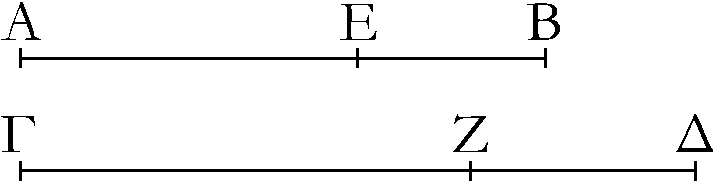
\includegraphics{Book10/fig066g.pdf}}

\gr{>'Εστω <ρητὸν καὶ μέσον δυναμένη ἡ ΑΒ, καὶ τῆ|
ΑΒ σύμμετροξ >έστω ἡ ΓΔ; δεικτέον, <ότι καὶ ἡ ΓΔ
<ρητὸν καὶ μέσον δυναμένη ἐστίν.}

\gr{Διῃρήσθω ἡ ΑΒ εἰξ τὰξ εὐθείαξ κατὰ τὸ Ε; αἱ ΑΕ, ΕΒ >άρα
δυνάμει εἰσὶν ἀσύμμετροι ποιοῦσαι
τὸ μὲν συγκείμενον ἐκ τῶν ἀπ> α\kern -.7pt  ὐτῶν τετραγώνων
μέσον, τὸ δ> ὑπ> α\kern -.7pt  ὐτῶν <ρητόν; καὶ τὰ α\kern -.5pt  ὐτὰ κατεσκευάσθω
τοῖξ πρότερον. ὁμοίωξ δὴ δείχομεν, <ότι καὶ αἱ ΓΖ,
ΖΔ δυνάμει εἰσὶν ἀσύμμετροι, καὶ σύμμετρον τὸ μὲν
συγκείμενον ἐκ τῶν ἀπὸ τῶν ΑΕ, ΕΒ τῶ| συγκειμένῳ
ἐκ τῶν ἀπὸ τῶν ΓΖ, ΖΔ, τὸ δὲ ὑπὸ ΑΕ, ΕΒ τῶ|
ὑπὸ ΓΖ, ΖΔ; <ώστε καὶ τὸ [μὲν] συγκείμενον ἐκ τῶν
ἀπὸ τῶν ΓΖ, ΖΔ τετραγώνων ἐστὶ μέσον, τὸ δ> ὑπὸ
τῶν ΓΖ, ΖΔ <ρητόν.}

\gr{<Ρητὸν >άρα καὶ μέσον δυναμένη ἐστὶν ἡ ΓΔ; <όπερ
>έδει δεῖχαι.}}

\ParallelRText{
\begin{center}
{\large Proposition 69}
\end{center}

A (straight-line) commensurable (in length)
with the square-root of a rational plus a medial (area) is [itself also]
the square-root of a rational plus a medial (area).

% Removed epsf size command
\centerline{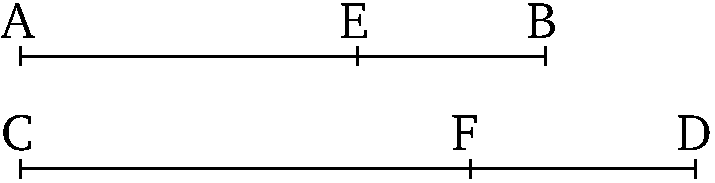
\includegraphics{Book10/fig066e.pdf}}

Let $AB$ be the square-root of a rational plus a medial (area), 
and let $CD$ be commensurable (in length) with $AB$. We must  show
that $CD$ is also the square-root of a rational plus a medial (area).

Let $AB$ be divided into its (component) straight-lines at $E$.
$AE$ and $EB$ are thus incommensurable in square, making 
the sum of the squares on them medial, and the (rectangle contained)
by them rational [Prop.~10.40]. And let the
same construction be made as in the previous (propositions).
So, similarly, we can show that $CF$ and $FD$ are also incommensurable
in square, and that the sum of the (squares) on $AE$ and $EB$
(is) commensurable with the sum of the (squares) on $CF$ and $FD$,
and the (rectangle contained) by $AE$ and $EB$ with the
(rectangle contained) by $CF$ and $FD$. And hence the sum of the
squares on $CF$ and $FD$ is medial, and the (rectangle contained) by
$CF$ and $FD$ (is) rational.

Thus, $CD$ is the square-root of a rational plus a medial (area) [Prop.~10.40]. (Which is) the very thing it was required to show.}
\end{Parallel}

%%%%
%10.70
%%%%
\pdfbookmark[1]{Proposition 10.70}{pdf10.70}
\begin{Parallel}{}{}
\ParallelLText{
\begin{center}
{\large \ggn{70}.}
\end{center}\vspace*{-7pt}

\gr{Ἡ τῆ| δύο μέσα δυναμένῃ σύμμετροξ δύο μέσα δυναμένη ἐστίν.}


\gr{>'Εστω δύο μέσα δυναμένη ἡ ΑΒ, καὶ τῆ| ΑΒ σύμμετροξ
ἡ ΓΔ; δεικτέον, <ότι καὶ ἡ ΓΔ δύο μέσα δυναμένη ἐστίν.}\\~\\~\\

% Removed epsf size command
\centerline{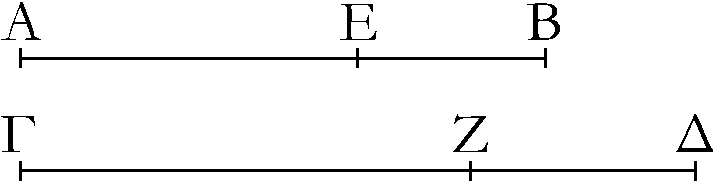
\includegraphics{Book10/fig066g.pdf}}
\gr{Ἐπεὶ γὰρ δύο μέσα δυναμένη ἐστὶν ἡ ΑΒ, διῃρήσθω
εἰξ τὰξ εὐθείαξ κατὰ τὸ Ε; αἱ ΑΕ, ΕΒ >άρα δυνάμει εἰσὶν
ἀσύμμετροι ποιοῦσαι τό τε συγκείμενον ἐκ τῶν ἀπ> α\kern -.7pt  ὐτῶν
[τετραγώνων] μέσον καὶ τὸ ὑπ> α\kern -.7pt  ὐτῶν μέσον καὶ >έτι
ἀσύμμετρον τὸ συγκείμενον ἐκ τῶν ἀπὸ τῶν ΑΕ, ΕΒ
τετραγώνων τῶ| ὑπὸ τῶν ΑΕ, ΕΒ; καὶ κατεσκευάσθω τὰ α\kern -.5pt  ὐτὰ
τοῖξ πρότερον. ὁμοίωξ δὴ δείχομεν, <ότι καὶ αἱ ΓΖ, ΖΔ δυνάμει
εἰσὶν ἀσύμμετροι καὶ σύμμετρον τὸ μὲν συγκείμενον ἐκ
τῶν ἀπὸ τῶν ΑΕ, ΕΒ τῶ| συγκειμένῳ ἐκ τῶν ἀπὸ τῶν
ΓΖ, ΖΔ, τὸ δὲ ὑπὸ τῶν ΑΕ, ΕΒ τῶ| ὑπὸ τῶν ΓΖ, ΖΔ;
<ώστε καὶ τὸ συγκείμενον ἐκ τῶν ἀπὸ τῶν ΓΖ, ΖΔ
 τετραγώνων
μέσον ἐστὶ καὶ τὸ ὑπὸ τῶν ΓΖ, ΖΔ μέσον καὶ >έτι ἀσύμμετρον
τὸ συγκείμενον ἐκ τῶν ἀπὸ τῶν ΓΖ, ΖΔ τετραγώνων τῶ| ὑπὸ
τῶν ΓΖ, ΖΔ.}

\gr{Ἡ >άρα ΓΔ δύο μέσα δυναμένη ἐστίν; <όπερ >έδει δεῖχαι.}}

\ParallelRText{
\begin{center}
{\large Proposition 70}
\end{center}

A (straight-line) commensurable (in length)
with the square-root of (the sum of) two medial (areas) is (itself also)
the square-root of (the sum of) two medial (areas).

Let $AB$ be the square-root of (the sum of) two medial (areas),
and (let) $CD$ (be) commensurable (in length) with $AB$. We must show that
$CD$ is also the square-root of (the sum of) two medial (areas).

% Removed epsf size command
\centerline{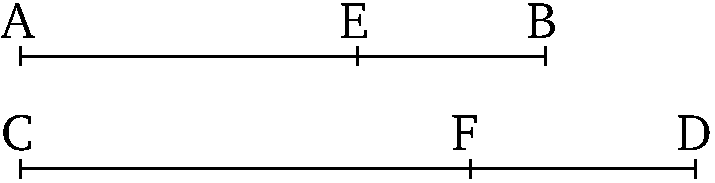
\includegraphics{Book10/fig066e.pdf}}

For since $AB$ is the square-root of (the sum of) two medial (areas),
let it be divided into its (component) straight-lines at $E$.
Thus, $AE$ and $EB$ are incommensurable in square, making the sum of
the [squares] on them medial, and the (rectangle contained) by them
medial, and, moreover, the sum of the (squares) on $AE$ and $EB$
incommensurable with the (rectangle) contained by $AE$ and $EB$ [Prop.~10.41]. And let the same construction
be made as in the previous (propositions). So, similarly, we
can show that $CF$ and $FD$ are also incommensurable in square,
and (that) the sum of the (squares) on $AE$ and $EB$ (is)
commensurable with the sum of the (squares) on $CF$ and $FD$, and the
(rectangle contained) by $AE$ and $EB$ with the (rectangle contained)
by $CF$ and $FD$. Hence, the sum of the squares on $CF$ and
$FD$ is also medial, and the (rectangle contained) by $CF$ and $FD$
(is) medial, and, moreover, the sum of the squares on $CF$ and $FD$
(is) incommensurable with the (rectangle contained) by $CF$ and $FD$.

Thus, $CD$ is the square-root of (the sum of) two medial (areas) [Prop.~10.41].
(Which is) the very thing it was required to show.}
\end{Parallel}

%%%%
%10.71
%%%%
\pdfbookmark[1]{Proposition 10.71}{pdf10.71}
\begin{Parallel}{}{}
\ParallelLText{
\begin{center}
{\large \ggn{71}.}
\end{center}\vspace*{-7pt}

\gr{<Ρητοῦ καὶ μέσου συντιθεμένου τέσσαρεξ >άλογοι γίγνον\-ται
>ήτοι ἐκ δύο ὀνομάτων >ὴ ἐκ δύο μέσων πρώτη >ὴ
μείζων >ὴ <ρητὸν καὶ μέσον δυναμένη.}

\gr{>'Εστω <ρητὸν μὲν τὸ ΑΒ, μέσον δὲ τὸ ΓΔ; λέγω, <ότι ἡ τὸ
ΑΔ θωρίον δυναμένη >ήτοι ἐκ δύο ὀνομάτων ἐστὶν
>ὴ ἐκ δύο μέσων πρώτη >ὴ μείζων >ὴ <ρητὸν καὶ
μέσον δυναμένη.}

\gr{Τὸ γὰρ ΑΒ τοῦ ΓΔ >ήτοι μεῖζόν ἐστιν >ὴ >έλασσον.
>έστω πρότερον μεῖζον; καὶ ἐκκείσθω <ρητὴ ἡ ΕΖ, καὶ
παραβεβλήσθω παρὰ τὴν ΕΖ τῶ| ΑΒ >ίσον τὸ ΕΗ
πλάτοξ ποιοῦν τὴν ΕΘ; τῶ| δὲ ΔΓ >ίσον παρὰ τὴν ΕΖ παραβεβλήσθω
τὸ ΘΙ πλάτοξ ποιοῦν τὴν ΘΚ. καὶ ἐπεὶ <ρητόν ἐστι τὸ ΑΒ καί
ἐστιν >ίσον τῶ| ΕΗ, <ρητὸν >άρα καὶ τὸ ΕΗ. καὶ παρὰ [<ρητὴν]
τὴν ΕΖ παραβέβληται πλάτοξ ποιοῦν τὴν ΕΘ; ἡ ΕΘ >άρα <ρητή ἐστι
καὶ σύμμετροξ τῆ| ΕΖ μ\kern -.7pt  ήκει. πάλιν, ἐπεὶ μέσον ἐστὶ τὸ ΓΔ καί
ἐστιν >ίσον τῶ| ΘΙ, μέσον >άρα ἐστὶ καὶ τὸ ΘΙ. καὶ παρὰ <ρητὴν
τὴν ΕΖ παράκειται πλάτοξ ποιοῦν τὴν ΘΚ; <ρητὴ >άρα ἐστὶν ἡ ΘΚ
καὶ ἀσύμμετροξ τῆ| ΕΖ μ\kern -.7pt  ήκει. καὶ ἐπεὶ μέσον ἐστὶ τὸ ΓΔ,
<ρητὸν δὲ τὸ ΑΒ, ἀσύμμετρον >άρα ἐστὶ τὸ ΑΒ τῶ| ΓΔ; <ώστε
καὶ τὸ ΕΗ ἀσύμμετρόν ἐστι τῶ| ΘΙ. ὡξ δὲ τὸ ΕΗ πρὸξ τὸ ΘΙ,
ο<ύτωξ ἐστὶν ἡ ΕΘ πρὸξ τὴν ΘΚ; ἀσύμμετροξ >άρα ἐστὶ καὶ
ἡ ΕΘ τῆ| ΘΚ μ\kern -.5pt  ήκει. καί εἰσιν ἀμφότεραι <ρηταί; αἱ ΕΘ, ΘΚ
>άρα <ρηταί εἰσι δυνάμει μόνον σύμμετροι; ἐκ δύο >άρα
ὀνομάτων ἐστὶν ἡ ΕΚ διῃρημένη κατὰ τὸ Θ. καὶ ἐπεὶ
μεῖζόν ἐστι τὸ ΑΒ τοῦ ΓΔ, >ίσον δὲ τὸ μὲν ΑΒ τῶ| ΕΗ, τὸ δὲ
ΓΔ τῶ| ΘΙ, μεῖζον >άρα καὶ τὸ ΕΗ τοῦ ΘΙ; καὶ ἡ ΕΘ
>άρα μείζων ἐστὶ τῆξ ΘΚ. >ήτοι ο>ῦν ἡ ΕΘ τῆξ ΘΚ μεῖζον
δύναται τῶ| ἀπὸ συμμέτρου ἑαυτῆ| μ\kern -.3pt  ήκει >ὴ τῶ|
ἀπὸ ἀσυμμέτρου. δυνάσθω πρότερον τῶ| ἀπὸ συμμέτρου
ἑαυτῆ|; καί ἐστιν ἡ μείζων ἡ ΘΕ σύμμετροξ τῆ| ἐκκειμένῃ
<ρητῃ τῆ| ΕΖ; ἡ >άρα ΕΚ ἐκ δύο ὀνομάτων ἐστὶ πρώτη. <ρητὴ
δὲ ἡ ΕΖ; ἒαν δὲ θωρίον περιέθηται ὑπὸ <ρητῆξ καὶ τῆξ ἐκ
δύο ὀνομάτων πρώτηξ, ἡ τὸ θωρίον δυναμένη ἐκ δύο ὀνομάτων
ἐστίν. ἡ >άρα τὸ ΕΙ δυναμένη ἐκ δύο ὀνομάτων ἐστίν; <ώστε
καὶ ἡ τὸ ΑΔ δυναμένη ἐκ δύο ὀνομάτων ἐστίν. ἀλλὰ δὴ δυνάσθω
ἡ ΕΘ τῆξ ΘΚ μεῖζον τῶ| ἀπὸ ἀσυμμέτρου ἑαυτῆ|; καί
ἐστιν ἡ μείζων ἡ ΕΘ σύμμετροξ τῆ| ἐκκειμένῃ <ρητῆ|
τῆ| ΕΖ μ\kern -.7pt  ήκει; ἡ >άρα ΕΚ ἐκ δύο ὀνομάτων ἐστὶ τετάρτη.
<ρητὴ δὲ ἡ ΕΖ; ἒαν δὲ θωρίον περιέθηται ὑπὸ <ρητῆξ
καὶ τῆξ ἐκ δύο ὀνομάτων τετάρτηξ, ἡ τὸ θωρίον δυναμένη >άλογόξ
ἐστιν ἡ καλουμένη μείζων. ἡ >άρα τὸ ΕΙ θωρίον δυναμένη μείζων
ἐστίν; <ώστε καὶ ἡ τὸ ΑΔ δυναμένη μείζων ἐστίν.}

\gr{Ἀλλὰ δὴ >έστω >έλασσον τὸ ΑΒ τοῦ ΓΔ; καὶ τὸ ΕΗ >άρα >έλασσόν
ἐστι τοῦ ΘΙ; <ώστε καὶ ἡ ΕΘ ἐλάσσων ἐστὶ τῆξ ΘΚ. >ήτοι δὲ ἡ ΘΚ
τῆξ ΕΘ
 μεῖζον δύναται τῶ| ἀπὸ συμμέτρου
ἑαυτῆ| >ὴ τῶ| ἀπὸ ἀσυμμέτρου. δυνάσθω πρότερον τῶ| ἀπὸ
συμμέτρου ἑαυτῆ| μ\kern -.7pt  ήκει; καί ἐστιν ἡ ἐλάσσων ἡ ΕΘ σύμμετροξ
τῆ| ἐκκειμένῃ <ρητῆ| τῆ| ΕΖ μ\kern -.7pt  ήκει; ἡ >άρα ΕΚ ἐκ δύο
ὀνομάτων ἐστὶ δευτέρα. <ρητὴ δὲ ἡ ΕΖ; ἒαν δὲ θωρίον
περιέθηται ὑπὸ <ρητῆξ καὶ τῆξ ἐκ δύο ὀνομάτων δευτέραξ,
ἡ τὸ θωρίον δυναμένη ἐκ δύο μέσων ἐστὶ πρώτη. ἡ >άρα
τὸ ΕΙ θωρίον δυναμένη ἐκ δύο μέσων ἐστὶ πρώτη; <ώστε
καὶ ἡ τὸ ΑΔ δυναμένη ἐκ δύο μέσων ἐστὶ πρώτη. ἀλλὰ δὴ
ἡ ΘΚ τῆξ ΘΕ μεῖζον δυνάσθω τῶ| ἀπὸ ἀσυμμέτρου ἑαυτῆ|.
καί ἐστιν ἡ ἐλάσσων ἡ ΕΘ σύμμετροξ τῆ| ἐκκειμένῃ
<ρητῆ| τῆ| ΕΖ; ἡ >άρα ΕΚ ἐκ δύο ὀνομάτων ἐστὶ πέμπτη.
<ρητὴ δὲ ἡ ΕΖ; ἒαν δὲ θωρίον περιέθηται ὑπὸ <ρητῆξ καὶ τῆξ
ἐκ δύο ὀνομάτων πέμπτηξ, ἡ τὸ θωρίον δυναμένη <ρητὸν καὶ μέσον δυναμένη ἐστίν. ἡ >άρα τὸ ΕΙ θωρίον δυναμένη <ρητὸν
καὶ μέσον δυναμένη ἐστίν; <ώστε καὶ ἡ τὸ ΑΔ θωρίον δυναμένη
<ρητὸν καὶ μέσον δυναμένη ἐστίν.}\\~\\~\\~\\~\\~\\~\\~\\~\\~\\~\\~\\~\\~\\~\\~\\~\\~\\~\\~\\~\\~\\~\\~\\~\\~\\

% Removed epsf size command
\centerline{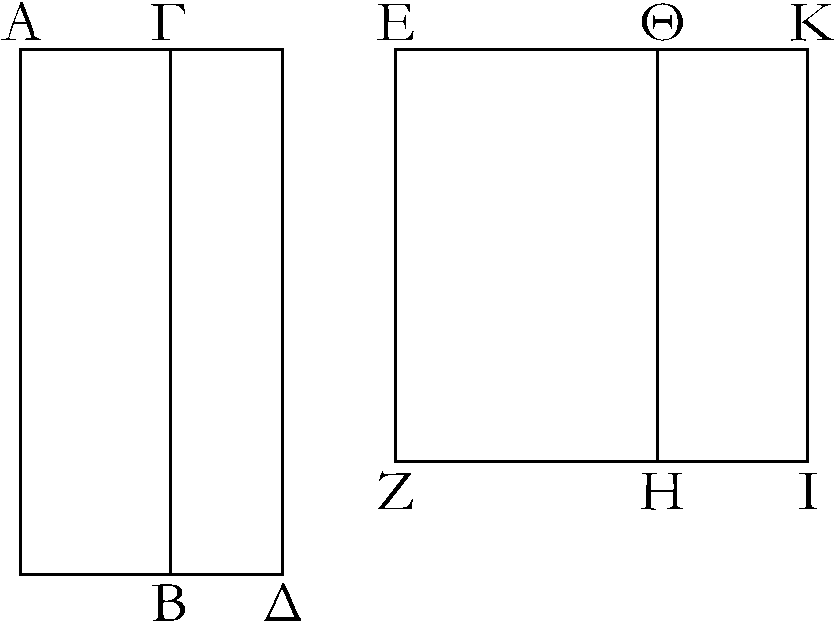
\includegraphics{Book10/fig071g.pdf}}

\gr{<Ρητοῦ >άρα καὶ μέσου συντιθεμένου τέσσαρεξ >άλογοι γίγνονται
>ήτοι ἐκ δύο ὀνομάτων >ὴ ἐκ δύο μέσων πρώτη >ὴ μείζων
>ὴ <ρητὸν καὶ μέσον δυναμένη; <όπερ >έδει δεῖχαι.}}

\ParallelRText{
\begin{center}
{\large Proposition 71}
\end{center}

When a rational and a medial (area) are added
together, four irrational (straight-lines) arise (as the square-roots of the
total area)---either a binomial, or a first bimedial, or a major, or the
square-root of a rational plus a medial (area).

Let $AB$ be a rational (area), and $CD$ a medial (area). I say that the
square-root of area $AD$ is either binomial, or first bimedial, or
major, or the square-root of a rational plus a medial (area).

For $AB$ is either greater or less than $CD$. Let it, first of all,
be greater. And let the rational (straight-line) $EF$ be laid down. And
let (the rectangle) $EG$, equal to $AB$, be applied to $EF$,
producing $EH$ as breadth. And let (the recatangle) $HI$, equal to $DC$,
be applied to $EF$, producing $HK$ as breadth. And since
$AB$ is rational, and is equal to $EG$, $EG$ is thus also rational. And it
has been applied to the [rational] (straight-line) $EF$, producing $EH$
as breadth. $EH$ is thus rational, and commensurable in length
with $EF$ [Prop.~10.20]. Again, since
$CD$ is medial, and is equal to $HI$, $HI$ is thus also medial. 
And it is applied to the rational (straight-line) $EF$, producing
$HK$ as breadth. $HK$ is thus rational, and incommensurable
in length with $EF$ [Prop.~10.22]. And since
$CD$ is medial, and $AB$ rational, $AB$ is thus incommensurable
with $CD$. Hence, $EG$ is also incommensurable with $HI$. And
as $EG$ (is) to $HI$, so $EH$ is to $HK$ [Prop.~6.1].
Thus, $EH$ is also incommensurable in length with $HK$
[Prop.~10.11]. And they are both rational. Thus,
$EH$ and $HK$ are rational (straight-lines which are) commensurable in
 square only. $EK$ is thus a binomial (straight-line), having been divided
(into its component terms) at $H$ [Prop.~10.36].
And since $AB$ is greater than $CD$, and $AB$ (is) equal to $EG$, and
$CD$ to $HI$, $EG$ (is) thus also greater than $HI$. Thus, $EH$
is also greater than $HK$ [Prop.~5.14]. Therefore,
 the square on $EH$ is greater than (the square on) $HK$
either by the (square) on (some straight-line) commensurable in length
with ($EH$), or by the (square) on (some straight-line)  incommensurable
(in length with $EH$). 
Let it, first of all, be greater by the (square) on (some straight-line)
commensurable (in length with $EH$). And the greater (of the two components of $EK$) $HE$ is commensurable
(in length) with the (previously) laid down (straight-line) $EF$. $EK$ is thus a first binomial
(straight-line) [Def.~10.5]. And $EF$ (is) rational. And if an area is contained by a rational (straight-line) and a first
binomial (straight-line) then the square-root  of the  area is a binomial
(straight-line)  [Prop.~10.54]. Thus,
the square-root of $EI$ is a binomial (straight-line). Hence the square-root of $AD$ is also a binomial (straight-line).  And, so, let the
 square on $EH$ be greater than (the square on) $HK$ by the (square) on 
 (some straight-line) incommensurable (in length) with ($EH$). And the
 greater (of the two components of $EK$) $EH$ is commensurable in length with the (previously)
 laid down rational (straight-line) $EF$. Thus, $EK$ is a fourth
 binomial (straight-line) [Def.~10.8]. And
 $EF$ (is) rational. And if an area
 is contained by a rational (straight-line) and a fourth binomial (straight-line) 
 then the square-root of the area is the irrational (straight-line) called
 major [Prop.~10.57]. Thus, the square-root
 of area $EI$ is a major (straight-line). Hence, the square-root of
 $AD$ is also major.

 And so, let $AB$ be less than $CD$. Thus, $EG$ is also less
 than $HI$. Hence, $EH$ is also less than $HK$ [Props.~6.1, 5.14].
 And the square on $HK$ is greater than (the square on) $EH$ either
 by the (square) on (some straight-line) commensurable (in length)
 with ($HK$), or by the (square) on (some straight-line) incommensurable
 (in length) with ($HK$). Let it, first of all, be greater by the square
 on (some straight-line) commensurable in length with ($HK$).
 And the lesser (of the two components of $EK$) $EH$ is  commensurable in length with the
 (previously) laid down rational (straight-line) $EF$. Thus, $EK$
 is a second binomial (straight-line) [Def.~10.6]. 
 And $EF$ (is) rational. And if an area is contained by a rational (straight-line)
 and a second binomial (straight-line)  then the square-root of the area is a
 first bimedial (straight-line) [Prop.~10.55]. 
 Thus, the square-root of area $EI$ is a first bimedial (straight-line).
 Hence, the square-root of $AD$ is also a first bimedial (straight-line).
 And so, let the square on $HK$ be greater than (the square on) $HE$
 by the (square) on (some straight-line) incommensurable (in length) with
 ($HK$). 
 And the lesser (of the two components of $EK$) $EH$ is commensurable (in length) with the (previously) laid down rational (straight-line) $EF$.  Thus, $EK$ is a fifth binomial
 (straight-line) [Def.~10.9]. And $EF$ (is) rational. And if an area is
 contained by a rational (straight-line) and a fifth binomial (straight-line) 
 then the square-root of the area is the square-root of a rational plus
 a medial (area) [Prop.~10.58]. Thus, the square-root of area $EI$ is the square-root of a rational plus a medial (area). Hence,
 the square-root of area $AD$ is also the square-root of a rational plus
 a medial (area).
 
% Removed epsf size command
\centerline{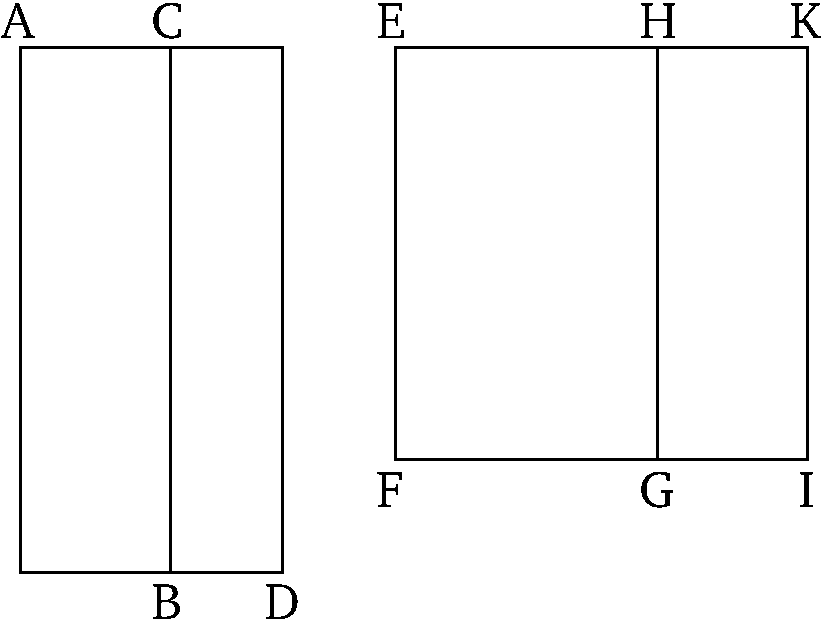
\includegraphics{Book10/fig071e.pdf}}

 Thus, when a rational and a medial area are added together, four irrational
(straight-lines) arise (as the square-roots of the
total area)---either a binomial, or a first bimedial, or a major, or the
square-root of a rational plus a medial (area). (Which is) the very thing
it was required to show.}
\end{Parallel}

%%%%
%10.72
%%%%
\pdfbookmark[1]{Proposition 10.72}{pdf10.72}
\begin{Parallel}{}{}
\ParallelLText{
\begin{center}
{\large \ggn{62}.}
\end{center}\vspace*{-7pt}

\gr{Δύο μέσων ἀσυμμέτρων ἀλλήλοιξ συντιθεμένων αἱ λοιπαὶ 
δύο >άλογοι γίγνονται >ήτοι ἐκ δύο μέσων δευτέρα >ὴ [ἡ]
δύο μέσα δυναμένη.}

\gr{Συγκείσθω γὰρ δύο μέσα ἀσύμμετρα ἀλλήλοιξ τὰ ΑΒ, ΓΔ; λέγω,
<ότι ἡ τὸ ΑΔ θωρίον δυναμένη >ήτοι ἐκ δύο μέσων
ἐστὶ δευτέρα >ὴ δύο μέσα δυναμένη.}

\gr{Τὸ γὰρ ΑΒ τοῦ ΓΔ >ήτοι μεῖζόν ἐστιν  >ὴ >έλασσον. >έστω,
εἰ τύθον, πρότερον μεῖζον τὸ ΑΒ τοῦ ΓΔ; καὶ ἐκκείσθω <ρητὴ
ἡ ΕΖ, καὶ τῶ| μὲν ΑΒ >ίσον παρὰ τὴν ΕΖ παραβεβλήσθω τὸ ΕΗ
πλάτοξ ποιοῦν τὴν ΕΘ, τῶ| δὲ ΓΔ >ίσον τὸ ΘΙ πλάτοξ ποιοῦν τὴν ΘΚ.
καὶ ἐπεὶ μέσον ἐστὶν ἑκάτερον τῶν ΑΒ, ΓΔ, μέσον
>άρα καὶ ἐκάτερον τῶν ΕΗ, ΘΙ. καὶ παρὰ <ρητὴν τὴν ΖΕ παράκειται
πλάτοξ ποιοῦν τὰξ ΕΘ, ΘΚ; ἑκατέρα >άρα τῶν ΕΘ, ΘΚ <ρητή
ἐστι καὶ ἀσύμμετροξ τῆ| ΕΖ μ\kern -.7pt  ήκει. καὶ ἐπεὶ ἀσύμμετρόν
ἐστι τὸ ΑΒ τῶ| ΓΔ, καί ἐστιν >ίσον τὸ μὲν ΑΒ τῶ| ΕΗ, 
τὸ δὲ ΓΔ τῶ| ΘΙ, ἀσύμμετρον >άρα ἐστὶ καὶ τὸ ΕΗ τῶ| ΘΙ.
ὡξ δὲ τὸ ΕΗ πρὸξ τὸ ΘΙ, ο<ύτωξ ἐστὶν ἡ ΕΘ
πρὸξ ΘΚ; ἀσύμμετροξ >άρα ἐστὶν ἡ ΕΘ τῆ| ΘΚ μ\kern -.7pt  ήκει. αἱ 
ΕΘ, ΘΚ >άρα <ρηταί εἰσι δυνάμει μόνον σύμμετροι; ἐκ
δύο >άρα ὀνομάτων ἐστὶν ἡ ΕΚ. >ήτοι δὲ ἡ ΕΘ τῆξ ΘΚ
μεῖζον δύναται τῶ| ἀπὸ συμμέτρου ἑαυτῆ| >ὴ τῶ| ἀπὸ
ἀσυμμέτρου. δυνάσθω πρότερον τῶ| ἀπὸ συμμέτρου ἑαυτῆ|
μ\kern -.5pt  ήκει; καὶ οὐδετέρα τῶν ΕΘ, ΘΚ σύμμετρόξ ἐστι τῆ| ἐκκειμένῃ
<ρητῆ| τῆ| ΕΖ μ\kern -.3pt  ήκει; ἡ ΕΚ >άρα ἐκ δύο ὀνομάτων ἐστὶ τρίτη.
<ρητὴ δὲ ἡ ΕΖ; ἒαν δὲ θωρίον περιέθηται ὑπὸ <ρητῆξ 
καὶ τῆξ ἐκ δύο ὀνομάτων τρίτηξ, ἡ τὸ θωρίον δυναμένη
ἐκ δύο μέσων ἐστὶ δευτέρα; ἡ >άρα τὸ ΕΙ, τουτέστι τὸ ΑΔ,
δυναμένη ἐκ δύο μέσων ἐστὶ δευτέρα. ἀλλα δὴ ἡ ΕΘ τῆξ ΘΚ
μεῖζον δυνάσθω τῶ| ἀπὸ ἀσυμμέτρου ἑαυτῆ| μ\kern -.7pt  ήκει; καὶ
ἀσύμμετρόξ ἐστιν ἑκατέρα τῶν ΕΘ, ΘΚ τῆ| ΕΖ μ\kern -.7pt  ήκει; ἡ >άρα
ΕΚ ἐκ δύο ὀνομάτων ἐστὶν <έκτη. ἒαν δὲ θωρίον περιέθηται
ὑπὸ <ρητῆξ καὶ τῆξ ἐκ δύο ὀνομάτων <έκτηξ, ἡ τὸ
θωρίον δυναμένη ἡ δύο μέσα δυναμένη ἐστίν; <ώστε καὶ ἡ
τὸ ΑΔ θωρίον δυναμένη ἡ δύο μέσα δυναμένη ἐστίν.}\\~\\~\\~\\~\\~\\~\\~\\~\\~\\~\\~\\~\\~\\

% Removed epsf size command
\centerline{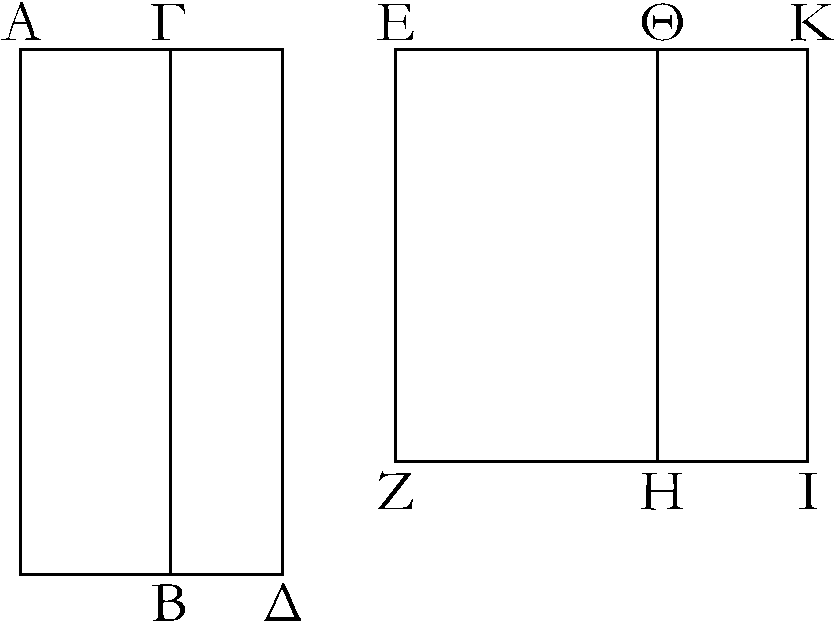
\includegraphics{Book10/fig071g.pdf}}

\gr{\kern -.7pt {[}<Omo'iwc d`h de'ixomen, <'oti k>`an >'elatton >~h| t`o AB
to~u GD, <h t`o AD qwr'ion dunam'enh >`h >ek d'uo m'eswn
deut'era >est`in >'htoi d'uo m'esa dunam'enh].}

\gr{Δύο >άρα μέσων ἀσυμμέτρων ἀλλήλοιξ συντιθεμένων αἱ λοιπαὶ
δύο >άλογοι γίγνονται >ήτοι ἐκ δύο μέσων δευτέρα >ὴ δύο μέσα
δυναμένη.}\\

\gr{Ἠ ἐκ δύο ὀνομάτων καὶ αἱ μετ> α\kern -.7pt  ὐτὴν >άλογοι ο>ύτε
τῆ| μέσῃ ο>ύτε ἀλλήλαιξ εἰσὶν αἱ α\kern -.7pt  ὐταί. τὸ μὲν γὰρ ἀπὸ
μέσηξ παρὰ <ρητὴν παραβαλλόμενον πλάτοξ ποιεῖ <ρητὴν καὶ
ἀσύμμετρον τῆ| παρ> <ὴν παράκειται μ\kern -.5pt  ήκει. τὸ δὲ ἀπὸ τῆξ
ἐκ δύο ὀνομάτων παρὰ <ρητὴν παραβαλλόμενον πλάτοξ ποιεῖ
τὴν ἐκ δύο ὀνομάτων πρώτην. τὸ δὲ ἀπὸ τῆξ ἐκ δύο μέσων
πρώτηξ παρὰ <ρητὴν παραβαλλόμενον πλάτοξ ποιεῖ τὴν ἐκ δύο
ὀνομάτων δευτέραν. τὸ δὲ ἀπὸ τῆξ ἐκ δύο μέσων δευτέραξ παρὰ
<ρητὴν παραβαλλόμενον πλάτοξ ποιεῖ τὴν ἐκ δύο ὀνομάτων
τρίτην. τὸ δὲ ἀπὸ τῆξ μείζονοξ παρὰ <ρητὴν παραβαλλόμενον
πλάτοξ ποιεῖ τὴν ἐκ δύο ὀνομάτων
τετάρτην. τὸ δὲ ἀπὸ τῆξ <ρητὸν καὶ μέσον δυναμένηξ
παρὰ <ρητὴν παραβαλλόμενον πλάτοξ ποιεῖ τὴν ἐκ δύο
ὀνομάτων πέμπτην. τὸ δὲ ἀπὸ τῆξ δύο μέσα δυναμένηξ
παρὰ <ρητὴν παραβαλλόμενον πλάτοξ ποιεῖ τὴν ἐκ δύο ὀνομάτων
<έκτην. τὰ δ> εἰρημένα πλάτη διαφέρει τοῦ τε πρώτου καὶ ἀλλήλων,
τοῦ μὲν πρώτου, <ότι <ρητή ἐστιν, ἀλλήλων δέ, <ότι τῆ| τάχει
οὐκ εἰσὶν αἱ α\kern -.3pt  ὐταί; <ώστε καὶ α\kern -.7pt  ὐταὶ αἱ >άλογοι διαφέρουσιν
ἀλλήλων.}}

\ParallelRText{
\begin{center}
{\large Proposition 72}
\end{center}

When two medial (areas which are) incommensurable with one another are added together, the remaining
two irrational (straight-lines) arise (as the square-roots of the total area)---either a second bimedial, or the square-root of (the sum of)
two medial (areas).

For let the two medial (areas) $AB$ and $CD$, (which are) incommensurable
with one another, be added together. I say that the square-root
of area $AD$ is either a second bimedial, or the square-root of (the sum of)
two medial (areas).

For $AB$ is either greater than or less than $CD$. By chance, let $AB$,
first of all,  be greater than $CD$. And let the rational (straight-line)
$EF$ be laid down. And let $EG$, equal to $AB$, be applied
to $EF$, producing $EH$ as breadth, and $HI$, equal to $CD$, producing
$HK$ as breadth. And since $AB$ and $CD$ are each medial,
$EG$ and $HI$ (are) thus also each medial. And they are applied to
the rational straight-line $FE$, producing $EH$ and $HK$ (respectively) as breadth. Thus, $EH$ and $HK$ are  each rational (straight-lines which are) incommensurable in length with $EF$ [Prop.~10.22]. And since $AB$ is incommensurable
with $CD$, and $AB$ is equal to $EG$, and $CD$ to $HI$, $EG$
is thus also incommensurable with $HI$. And as $EG$ (is) to $HI$,
so $EH$ is to $HK$ [Prop.~6.1].  $EH$ is thus
incommensurable in length with $HK$ [Prop.~10.11]. Thus, $EH$ and $HK$ are rational
(straight-lines which are) commensurable in square only. $EK$
is thus a binomial (straight-line) [Prop.~10.36]. 
And the square on $EH$ is  greater than (the square on) $HK$
either by the (square) on (some straight-line) commensurable (in length) with ($EH$), or
by the (square) on (some straight-line) incommensurable (in length
with $EH$). Let it, first of all, be greater by the square on (some
straight-line) commensurable in length with ($EH$). And neither of
$EH$ or $HK$ is commensurable in length with the (previously)
laid down rational (straight-line) $EF$.  Thus, $EK$ is a third
binomial (straight-line) [Def.~10.7]. And $EF$
(is) rational. And if an area is contained by a rational (straight-line) and
a third binomial (straight-line)  then the square-root of the area
is a second bimedial  (straight-line) [Prop.~10.56]. Thus,
the square-root of $EI$---that is to say, of $AD$---is a second bimedial.
And so, let the square on $EH$ be greater than (the square) on $HK$
by the (square)  on (some straight-line) incommensurable in length
with ($EH$).  And $EH$ and $HK$
are each incommensurable
in length with $EF$. Thus, $EK$ is a sixth binomial (straight-line)
[Def.~10.10]. And if an area
is contained by
a rational (straight-line) and a sixth binomial (straight-line)  then the square-root of the area is the square-root of (the sum of) two medial (areas) 
[Prop.~10.59]. Hence, the
square-root of area $AD$ is also the square-root of (the sum of)
two medial (areas).

% Removed epsf size command
\centerline{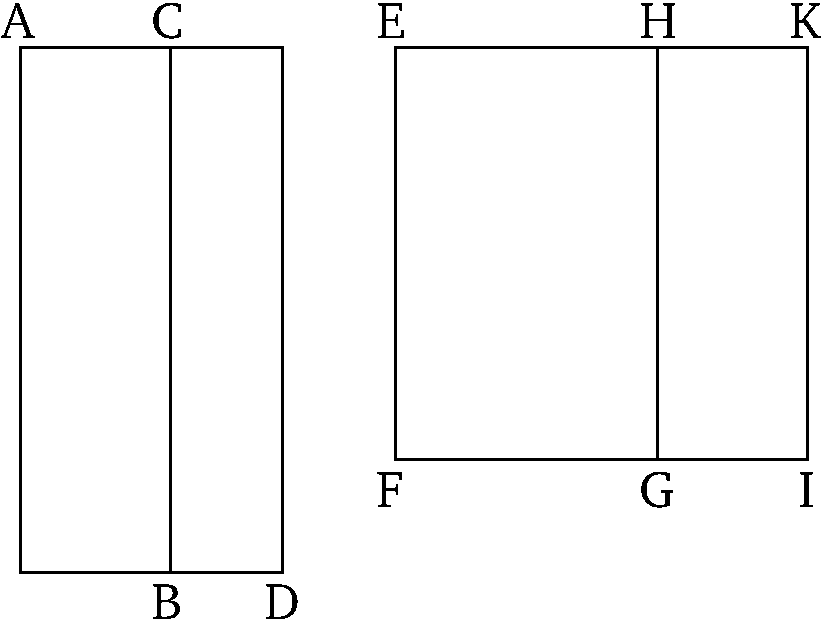
\includegraphics{Book10/fig071e.pdf}}

\mbox{[}So, similarly, we can show that, even if $AB$ is less than $CD$, the
square-root of area $AD$ is either a second bimedial or the square-root
of (the sum of) two medial (areas).]

Thus, when two medial (areas which are) incommensurable with one another are added together, the remaining
two irrational (straight-lines) arise (as the square-roots of the total area)---either a second bimedial, or the square-root of (the sum of)
two medial (areas).\\

A binomial (straight-line), and the (other) irrational (straight-lines) 
after it, are neither the same as a medial (straight-line) nor (the same) as one another.
For the (square) on a medial (straight-line), applied to a rational (straight-line),
produces as breadth a rational (straight-line which is) also incommensurable
in length with (the straight-line) to which it is applied [Prop.~10.22]. And the (square) on a binomial
(straight-line), applied to a rational (straight-line), produces
as breadth a first binomial [Prop.~10.60]. 
And the (square) on a first bimedial (straight-line), applied
to a rational (straight-line), produces as breadth a  second binomial
[Prop.~10.61]. And the (square) on a second bimedial (straight-line), applied
to a rational (straight-line), produces as breadth a  third binomial
[Prop.~10.62]. And the (square) on a major (straight-line), applied
to a rational (straight-line), produces as breadth a  fourth binomial
[Prop.~10.63].  And the (square) on the square-root of a rational plus a medial (area), applied
to a rational (straight-line), produces as breadth a  fifth binomial
[Prop.~10.64]. And the (square) on the square-root of (the sum of) two medial (areas), applied
to a rational (straight-line), produces as breadth a  sixth binomial
[Prop.~10.65]. And the aforementioned breadths
differ from the first (breadth), and from one another---from the first, because it is rational---and from one another, because they are not the same in order. Hence, the (previously mentioned) irrational (straight-lines) themselves
also differ from one another.}
\end{Parallel}

%%%%
%10.73
%%%%
\pdfbookmark[1]{Proposition 10.73}{pdf10.73}
\begin{Parallel}{}{}
\ParallelLText{
\begin{center}
{\large \ggn{73}.}
\end{center}\vspace*{-7pt}

\gr{Ἐὰν ἀπὸ <ρητῆξ <ρητὴ ἀφαιρεθῆ| δυνάμει μόνον σύμμετροξ ο>ῦσα
τῆ| <όλῃ, ἡ λοιπὴ >άλογόξ ἐστιν; καλείσθω δὲ ἀποτομ\kern -.7pt  ή.}\\~\\

% Removed epsf size command
\centerline{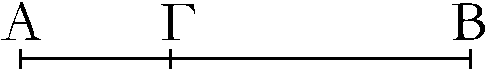
\includegraphics{Book10/fig073g.pdf}}

\gr{Ἀπὸ γὰρ <ρητῆξ τῆξ ΑΒ <ρητὴ ἀφῃρήσθω ἡ ΒΓ δυνάμει μόνον
σύμμετροξ ο>ῦσα τῆ| <όλῃ; λέγω, <ότι ἡ λοιπὴ ἡ ΑΓ >άλογόξ
ἐστιν ἡ καλουμένη ἀποτομ\kern -.7pt  ή.}

\gr{Ἐπεὶ γὰρ ἀσύμμετρόξ ἐστιν ἡ ΑΒ τῆ| ΒΓ μ\kern -.7pt  ήκει, καί ἐστιν
ὡξ ἡ ΑΒ πρὸξ τὴν ΒΓ, ο<ύτωξ τὸ ἀπὸ τῆξ ΑΒ πρὸξ τὸ ὑπὸ
τῶν ΑΒ, ΒΓ, ἀσύμμετρον >άρα ἐστὶ τὸ ἀπὸ τῆξ ΑΒ τῶ|
ὑπὸ τῶν ΑΒ, ΒΓ. ἀλλὰ τῶ| μὲν ἀπὸ τῆξ ΑΒ σύμμετρά ἐστι
τὰ ἀπὸ τῶν ΑΒ, ΒΓ τετράγωνα, τῶ| δὲ ὑπὸ τῶν ΑΒ, ΒΓ σύμμετρόν
ἐστι τὸ δὶξ ὑπὸ τῶν ΑΒ, ΒΓ. καὶ ἐπειδήπερ τὰ ἀπὸ τῶν ΑΒ, ΒΓ
>ίσα ἐστὶ τῶ| δὶξ ὑπὸ τῶν ΑΒ, ΒΓ μετὰ τοῦ ἀπὸ ΓΑ, καὶ
λοιπῶ| >άρα τῶ| ἀπὸ τῆξ ΑΓ ἀσύμμετρά ἐστι τὰ ἀπὸ τῶν ΑΒ, ΒΓ.
<ρητὰ δὲ τὰ ἀπὸ τῶν ΑΒ, ΒΓ; >άλογοξ >άρα ἐστὶν ἡ ΑΓ; καλείσθω
δὲ ἀποτομ\kern -.7pt  ή. <όπερ >έδει δεῖχαι.}}

\ParallelRText{
\begin{center}
{\large Proposition 73}
\end{center}

If  a  rational (straight-line), which is commensurable in square only with the
whole, is subtracted from a(nother) rational (straight-line)  then the remainder is an irrational (straight-line). Let it be called an apotome.

% Removed epsf size command
\centerline{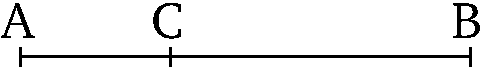
\includegraphics{Book10/fig073e.pdf}}

For let the rational (straight-line) $BC$, which commensurable in square only with the whole,  be subtracted from the
rational (straight-line) $AB$. I say that the remainder $AC$ is that irrational
(straight-line) called an apotome.

For since $AB$ is incommensurable in length with $BC$, and as $AB$ is to
$BC$, so the (square) on $AB$ (is) to the (rectangle contained) by $AB$ and
$BC$ [Prop.~10.21~lem.], the
(square) on $AB$ is thus incommensurable with the (rectangle contained)
by $AB$ and $BC$ [Prop.~10.11]. 
But, the (sum of the) squares on $AB$ and $BC$ is commensurable with the
(square) on $AB$ [Prop.~10.15], and twice
the (rectangle contained) by $AB$ and $BC$ is commensurable with the
(rectangle contained) by $AB$ and $BC$ [Prop.~10.6]. And, inasmuch as the (sum of the squares) on $AB$ and $BC$ is equal to twice the (rectangle contained) by
$AB$ and $BC$ plus the (square) on $CA$ [Prop.~2.7], the (sum of the squares) on $AB$ and $BC$
is thus also incommensurable with the remaining (square) on $AC$ [Props.~10.13, 10.16]. 
And the (sum of the squares) on $AB$ and $BC$ is rational. $AC$ is
thus an irrational (straight-line) [Def.~10.4]. And let it be called an
apotome.$^\dag$ (Which is) the very thing it was required to show.}
\end{Parallel}
{\footnotesize\noindent $^\dag$ See footnote to Prop.~10.36.}

%%%%
%10.74
%%%%
\pdfbookmark[1]{Proposition 10.74}{pdf10.74}
\begin{Parallel}{}{}
\ParallelLText{
\begin{center}
{\large \ggn{74}.}
\end{center}\vspace*{-7pt}

\gr{Ἐὰν ἀπὸ μέσηξ μέση ἀφαιρεθῆ| δυνάμει μόνον σύμμετροξ
ο>ῦσα τῆ| <όλῃ, μετὰ δὲ τῆξ <όληξ <ρητὸν περιέθουσα, ἡ λοιπὴ
>άλογόξ ἐστιν; καλείσθω δὲ μέσηξ ἀποτομ\kern -.7pt  ὴ πρώτη.}\\~\\~\\

% Removed epsf size command
\centerline{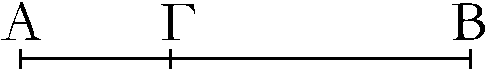
\includegraphics{Book10/fig073g.pdf}}

\gr{Ἀπὸ γὰρ μέσηξ τῆξ ΑΒ μέση ἀφῃρήσθω ἡ ΒΓ δυνάμει
μόνον σύμμετροξ ο>ῦσα τῆ| ΑΒ, μετὰ δὲ τῆξ ΑΒ <ρητὸν
ποιοῦσα τὸ ὑπὸ τῶν ΑΒ, ΒΓ; λέγω, <ότι
ἡ λοιπὴ ἡ ΑΓ >άλογόξ ἐστιν; καλείσθω δὲ μέσηξ ἀποτομ\kern -.7pt  ὴ
πρώτη.}

\gr{Ἐπεὶ γὰρ αἱ  ΑΒ, ΒΓ μέσαι εἰσίν, μέσα ἐστὶ καὶ τὰ ἀπὸ τῶν
ΑΒ, ΒΓ. <ρητὸν δὲ τὸ δὶξ ὑπὸ τῶν ΑΒ, ΒΓ; ἀσύμμετρα >άρα τὰ
ἀπὸ τῶν ΑΒ, ΒΓ τῶ| δὶξ ὑπὸ
τῶν ΑΒ, ΒΓ; καὶ λοιπῶ| >άρα τῶ| ἀπὸ τῆξ ΑΓ ἀσύμμετρόν ἐστι
τὸ δὶξ ὑπὸ τῶν ΑΒ, ΒΓ, ἐπεὶ κ>ὰν τὸ <όλον ἑνὶ α\kern -.7pt  ὐτῶν
ἀσύμμετρον >ῆ|, καὶ τὰ ἐχ ἀρθῆξ μεγέθη ἀσύμμετρα >έσται.
<ρητὸν δὲ τὸ δὶξ ὑπὸ τῶν ΑΒ, ΒΓ;
>άλογον >άρα τὸ ἀπὸ τῆξ ΑΓ; >άλογοξ >άρα ἐστὶν ἡ ΑΓ;
καλείσθω δὲ μέσηξ ἀποτομ\kern -.7pt  ὴ πρώτη.}}

\ParallelRText{
\begin{center}
{\large Proposition 74}
\end{center}

If  a medial (straight-line), which is commensurable in square only
with the whole, and which contains a rational (area) with the whole,  is subtracted from a(nother) medial
(straight-line)   then
the remainder is an irrational (straight-line). Let it be called a
first  apotome of a medial (straight-line).

% Removed epsf size command
\centerline{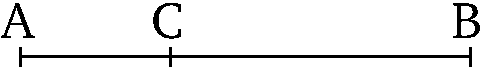
\includegraphics{Book10/fig073e.pdf}}

For let the medial (straight-line) $BC$, which is commensurable in square only with $AB$,
and which makes with $AB$ the rational (rectangle contained) by $AB$ and $BC$,
be subtracted from the medial (straight-line) $AB$ [Prop.~10.27]. I say that
the remainder $AC$ is an irrational (straight-line). Let it be
called the first apotome of a medial (straight-line).

For since $AB$ and $BC$ are medial (straight-lines), the (sum of the squares)
on $AB$ and $BC$ is also medial. And twice the (rectangle contained)
by $AB$ and $BC$ (is) rational. The (sum of the squares) on $AB$
and $BC$ (is) thus incommensurable with twice the (rectangle contained)
by $AB$ and $BC$. Thus, twice the (rectangle contained) by
$AB$ and $BC$ is also incommensurable with the remaining (square) on $AC$ [Prop.~2.7], since  if the whole is
incommensurable with one of the (constituent magnitudes)   then the original magnitudes will also be incommensurable (with one another) [Prop.~10.16]. And twice the (rectangle
contained) by $AB$ and $BC$ (is) rational. Thus, the (square) on $AC$
is irrational. Thus, $AC$ is an irrational (straight-line) [Def.~10.4]. Let it be called a first apotome
of a medial (straight-line).$^\dag$}
\end{Parallel}
{\footnotesize\noindent $^\dag$ See footnote to Prop.~10.37.} 

%%%%
%10.75
%%%%
\pdfbookmark[1]{Proposition 10.75}{pdf10.75}
\begin{Parallel}{}{}
\ParallelLText{
\begin{center}
{\large \ggn{75}.}
\end{center}\vspace*{-7pt}

\gr{Ἐὰν ἀπὸ μέσηξ μέση ἀφαιρεθῆ| δυνάμει μόνον σύμμετροξ
ο>ῦσα τῆ| <όλη, μετὰ δὲ τῆξ <όληξ μέσον περιέθουσα, ἡ
λοιπὴ >άλογόξ ἐστιν; καλείσθω δὲ μέσηξ ἀποτομ\kern -.7pt  ὴ δευτέρα.}

\gr{Ἀπὸ γὰρ μέσηξ τῆξ ΑΒ μέση ἀφῃρήσθω ἡ ΓΒ δυνάμει μόνον
σύμμετροξ ο>ῦσα τῆ| <όλῃ τῆ| ΑΒ, μετὰ δὲ τῆξ <όληξ τῆξ ΑΒ
μέσον περιέθουσα τὸ ὑπὸ τῶν ΑΒ, ΒΓ; λέγω, <ότι
ἡ λοιπὴ ἡ ΑΓ >άλογόξ ἐστιν; καλείσθω δὲ μέσηξ ἀποτομ\kern -.7pt  ὴ
δευτέρα.}\\~\\~\\~\\~\\

% Removed epsf size command
\centerline{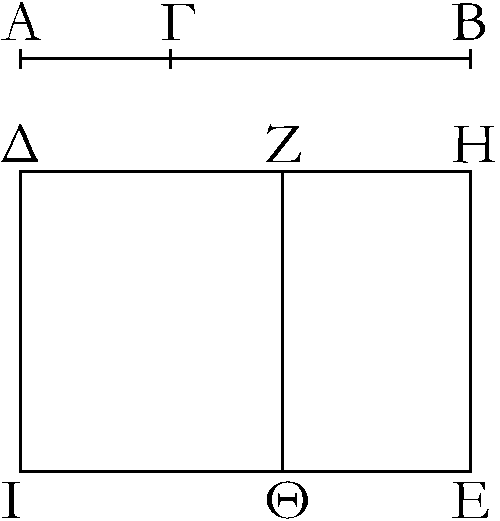
\includegraphics{Book10/fig075g.pdf}}

\gr{Ἐκκείσθω γὰρ <ρητὴ ἡ ΔΙ, καὶ τοῖξ μὲν ἀπὸ τῶν
ΑΒ, ΒΓ >ίσον παρὰ τὴν ΔΙ παραβεβλήσθω τὸ ΔΕ
πλάτοξ ποιοῦν τὴν ΔΗ, τῶ| δὲ δὶξ ὑπὸ τῶν ΑΒ, ΒΓ
>ίσον παρὰ τὴν ΔΙ παραβεβλήσθω τὸ ΔΘ πλάτοξ ποιοῦν τὴν
ΔΖ; λοιπὸν >άρα τὸ ΖΕ >ίσον ἐστὶ τῶ| ἀπὸ τῆξ ΑΓ.
καὶ ἐπεὶ μέσα καὶ σύμμετρά ἐστι τὰ ἀπὸ τῶν ΑΒ, ΒΓ,
μέσον >άρα καὶ τὸ ΔΕ. καὶ παρὰ <ρητὴν τὴν ΔΙ παράκειται
πλάτοξ ποιοῦν τὴν ΔΗ; <ρητὴ >άρα ἐστὶν ἡ ΔΗ καὶ ἀσύμμετροξ
τῆ| ΔΙ μ\kern -.7pt  ήκει. πάλιν, ἐπεὶ μέσον ἐστὶ τὸ ὑπὸ τῶν ΑΒ, ΒΓ, καὶ
τὸ δὶξ >άρα ὑπὸ τῶν ΑΒ, ΒΓ μέσον ἐστίν. καί ἐστιν >ίσον
τῶ| ΔΘ; καὶ τὸ ΔΘ >άρα μέσον ἐστίν. καὶ παρὰ <ρητὴν τὴν ΔΙ
παραβέβληται πλάτοξ ποιοῦν τὴν ΔΖ; <ρητὴ >άρα ἐστὶν ἡ ΔΖ
καὶ ἀσύμμετροξ τῆ| ΔΙ μ\kern -.7pt  ήκει. καὶ ἐπεὶ αἱ ΑΒ, ΒΓ δυνάμει
μόνον σύμμετροί εἰσιν, ἀσύμμετροξ >άρα ἐστὶν ἡ ΑΒ
τῆ| ΒΓ μ\kern -.5pt  ήκει; ἀσύμμετρον >άρα καὶ τὸ ἀπὸ τῆξ ΑΒ
τετράγωνον τῶ| ὑπὸ τῶν ΑΒ, ΒΓ. ἀλλὰ τῶ| μὲν ἀπὸ
τῆξ ΑΒ σύμμετρά ἐστι τὰ ἀπὸ τῶν ΑΒ, ΒΓ, τῶ| δὲ ὑπὸ
τῶν ΑΒ, ΒΓ σύμμετρόν ἐστι τὸ δὶξ ὑπὸ τῶν ΑΒ, ΒΓ;
ἀσύμμετρον >άρα ἐστὶ τὸ δὶξ ὑπὸ τῶν ΑΒ, ΒΓ τοῖξ
ἀπὸ τῶν ΑΒ, ΒΓ. >ίσον δὲ τοῖξ μὲν ἀπὸ τῶν ΑΒ, ΒΓ
τὸ ΔΕ, τῶ| δὲ δὶξ ὑπὸ τῶν ΑΒ, ΒΓ τὸ ΔΘ; ἀσύμμετρον
>άρα [ἐστὶ] τὸ ΔΕ τῶ| ΔΘ. ὡξ δὲ τὸ ΔΕ πρὸξ τὸ ΔΘ,
ο<ύτωξ ἡ ΗΔ πρὸξ τὴν ΔΖ; ἀσύμμετροξ >άρα ἐστὶν ἡ ΗΔ
τῆ| ΔΖ. καί εἰσιν ἀμφότεραι <ρηταί; αἱ >άρα ΗΔ, ΔΖ
<ρηταί εἰσι δυνάμει μόνον σύμμετροι; ἡ ΖΗ >άρα ἀποτομ\kern -.3pt  ή
ἐστιν. <ρητὴ δὲ ἡ ΔΙ; τὸ δὲ ὑπὸ <ρητῆξ καὶ ἀλόγου
περιεχόμενον >άλογόν ἐστιν, καὶ ἡ δυναμένη α\kern -.7pt  ὐτὸ
>άλογόξ ἐστιν. καὶ δύναται τὸ ΖΕ ἡ ΑΓ; ἡ ΑΓ >άρα >άλογόξ
ἐστιν; καλείσθω δὲ μέσηξ ἀποτομ\kern -.7pt  ὴ δευτέρα. <όπερ
>έδει δεῖχαι.}}

\ParallelRText{
\begin{center}
{\large Proposition 75}
\end{center}

If  a medial (straight-line), which is commensurable in square only
with the whole, and which contains a medial (area) with the whole, is subtracted from a(nother) medial
(straight-line)   then
the remainder is an irrational (straight-line). Let it be called a second apotome of a medial (straight-line).

For let the medial (straight-line) $CB$, which is commensurable in square
only with the whole, $AB$, and which contains with the whole, $AB$, the
medial (rectangle contained) by $AB$ and $BC$, be subtracted from the medial (straight-line) $AB$ [Prop.~10.28].  I say that the remainder $AC$ is an
irrational (straight-line). Let it be called a second apotome of a medial (straight-line).

% Removed epsf size command
\centerline{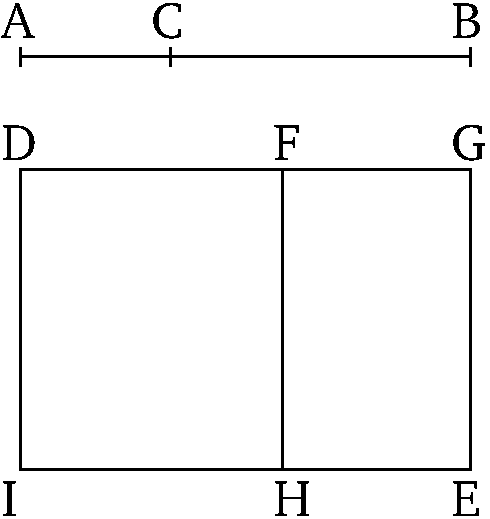
\includegraphics{Book10/fig075e.pdf}}

For let the rational (straight-line) $DI$ be laid down. And let $DE$, equal
to the (sum of the squares) on $AB$ and $BC$, be applied to
$DI$, producing $DG$ as breadth. And let $DH$, equal to twice the
(rectangle contained) by $AB$ and $BC$, be applied to $DI$,
producing $DF$ as breadth. The remainder $FE$ is thus equal to the
(square) on $AC$ [Prop.~2.7]. And since the
(squares) on $AB$ and $BC$ are medial and commensurable (with one another), $DE$ (is) thus also medial [Props.~10.15, 10.23~corr.]. And it is applied to the
rational (straight-line) $DI$, producing $DG$ as breadth. Thus, $DG$
is rational, and incommensurable in length with $DI$ [Prop.~10.22].  Again, since the (rectangle contained)
by $AB$ and $BC$ is medial, twice the (rectangle contained) by $AB$
and $BC$ is thus also medial [Prop.~10.23~corr.]. 
And it is equal to $DH$. Thus, $DH$ is also medial. And it has been
applied to the rational (straight-line) $DI$, producing $DF$ as breadth.
$DF$ is thus rational, and incommensurable in length with $DI$
[Prop.~10.22].  And since $AB$ and $BC$ are commensurable in square only, $AB$ is thus incommensurable in length
with $BC$. Thus, the square on $AB$ (is) also incommensurable
with the (rectangle contained) by $AB$ and $BC$ [Props.~10.21~lem.,
10.11]. But, the (sum of the squares) on $AB$ and $BC$  is commensurable with the (square) on $AB$  [Prop.~10.15], and twice the (rectangle contained)
by $AB$ and $BC$ is commensurable with the (rectangle contained)
by $AB$ and $BC$ [Prop.~10.6]. Thus, twice
the (rectangle contained) by $AB$ and $BC$ is incommensurable
with the (sum of the squares) on $AB$ and $BC$ [Prop.~10.13]. And $DE$ is equal
to the (sum of the squares) on $AB$ and $BC$, and $DH$ to
twice the (rectangle contained) by $AB$ and $BC$. Thus, $DE$
[is] incommensurable with $DH$. And as $DE$ (is) to $DH$, so
$GD$ (is) to $DF$ [Prop.~6.1]. Thus,
$GD$ is incommensurable with $DF$ [Prop.~10.11]. And they are both rational (straight-lines). Thus, $GD$ and $DF$ are rational (straight-lines which are)
commensurable in square only.
Thus, $FG$ is an apotome [Prop.~10.73]. 
And $DI$ (is) rational. And the (area) contained by a rational and
an irrational (straight-line) is irrational [Prop.~10.20], and its square-root 
is irrational. And $AC$ is the square-root of $FE$. Thus, $AC$ is an
irrational (straight-line) [Def.~10.4]. And
let it be called the second apotome of a medial (straight-line).$^\dag$
(Which is) the very thing it
was required to show.}
\end{Parallel}
{\footnotesize\noindent$^\dag$ See footnote to Prop.~10.38.} 

%%%%
%10.76
%%%%
\pdfbookmark[1]{Proposition 10.76}{pdf10.76}
\begin{Parallel}{}{}
\ParallelLText{
\begin{center}
{\large \ggn{76}.}
\end{center}\vspace*{-7pt}

\gr{Ἐὰν ἀπὸ εὐθείαξ εὐθεῖα ἀφαιρεθὴ| δυνάμει ἀσύμμετ\-ροξ
ο>ῦσα τῆ| <όλῃ, μετὰ δὲ τῆξ <όληξ ποιοῦσα τὰ μὲν ἀπ>
α\kern -.7pt  ὐτῶν <άμα <ρητόν, τὸ δ> ὑπ> α\kern -.7pt  ὐτῶν μέσον, ἡ λοιπὴ
>άλογόξ ἐστιν; καλείσθω δὲ ἐλάσσων.}\\~\\

% Removed epsf size command
\centerline{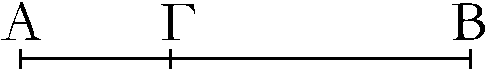
\includegraphics{Book10/fig073g.pdf}}

\gr{Ἀπὸ γὰρ εὐθείαξ τῆξ ΑΒ εὐθεῖα ἀφῃρήσθω ἡ ΒΓ δυνάμει
ἀσύμμετροξ ο>ῦσα τῆ| <όλῃ ποιοῦσα τὰ προκείμενα. λέγω,
<ότι ἡ λοιπὴ ἡ ΑΓ >άλογόξ ἐστιν ἡ καλουμένη ἐλάσσων.}

\gr{Ἐπεὶ γὰρ τὸ μὲν συγκείμενον ἐκ τῶν ἀπὸ τῶν ΑΒ, ΒΓ τετραγώνων <ρητόν ἐστιν, τὸ δὲ δὶξ ὑπὸ τῶν ΑΒ, ΒΓ μέσον,
ἀσύμμετρα >άρα ἐστὶ τὰ ἀπὸ τῶν ΑΒ, ΒΓ τῶ| δὶξ ὑπὸ
τῶν ΑΒ, ΒΓ; καὶ ἀναστρέψαντι λοιπῶ| τῶ| ἀπὸ τῆξ ΑΓ
ἀσύμμετρά ἐστι τὰ ἀπὸ τῶν ΑΒ, ΒΓ.  <ρητὰ δὲ τὰ
ἀπὸ τῶν ΑΒ, ΒΓ;
>άλογον >άρα
τὸ ἀπὸ τῆξ ΑΓ;
 >άλογοξ
>άρα ἡ ΑΓ; καλείσθω δὲ ἐλάσσων. <όπερ >έδει δεῖχαι.}}

\ParallelRText{
\begin{center}
{\large Proposition 76}
\end{center}

If  a straight-line, which is incommensurable in square with the whole,
and  with the whole makes the (squares) on them (added) together rational, and the
(rectangle contained) by them medial, is subtracted from a(nother) straight-line
 then the remainder is an
irrational (straight-line). Let it be called a minor (straight-line).

% Removed epsf size command
\centerline{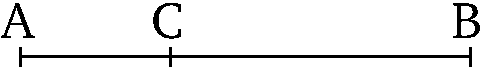
\includegraphics{Book10/fig073e.pdf}}

For let the straight-line $BC$, which is incommensurable in square with the whole, and fulfils the (other) prescribed (conditions), be subtracted from
the straight-line $AB$ [Prop.~10.33]. I say that the remainder $AC$ is that irrational (straight-line)
called minor.

For since the sum of the squares on $AB$ and $BC$ is rational, and twice
the (rectangle contained) by $AB$ and $BC$ (is) medial, the (sum of the squares) on $AB$ and $BC$ is thus incommensurable with twice the
(rectangle contained) by $AB$ and $BC$. And, via conversion, 
the (sum of the squares) on $AB$ and $BC$ is incommensurable with the
remaining (square) on $AC$ [Props.~2.7, 10.16]. And the (sum of the squares) on $AB$
and $BC$ (is) rational. The (square) on $AC$ (is) thus irrational. Thus, 
$AC$ (is) an irrational (straight-line) [Def.~10.4]. Let it be
called a minor (straight-line).$^\dag$ (Which is) the very thing it
was required to show.}
\end{Parallel}
{\footnotesize\noindent$^\dag$ See footnote to Prop.~10.39.}

%%%%
%10.77
%%%%
\pdfbookmark[1]{Proposition 10.77}{pdf10.77}
\begin{Parallel}{}{}
\ParallelLText{
\begin{center}
{\large \ggn{77}.}
\end{center}\vspace*{-7pt}

\gr{Ἐὰν ἀπὸ εὐθείαξ εὐθεῖα ἀφαιρεθῆ| δυνάμει ἀσύμμετ\-ροξ
ο>ῦσα τῆ| <όλῃ, μετὰ δὲ τῆξ <όληξ ποιοῦσα τὸ μὲν συγκείμενον
ἐκ τῶν ἀπ> α\kern -.7pt  ὐτῶν τετραγώνων μέσον, τὸ δὲ δὶξ ὑπ>
α\kern -.7pt  ὐτῶν <ρητόν, ἡ λοιπὴ >άλογόξ ἐστιν; καλείσθω δὲ ἡ μετὰ <ρητοῦ
μέσον τὸ <όλον ποιοῦσα.}\\

% Removed epsf size command
\centerline{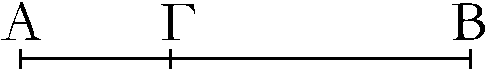
\includegraphics{Book10/fig073g.pdf}}

\gr{Ἀπὸ γὰρ εὐθείαξ τῆξ ΑΒ εὐθεῖα ἀφῃρήσθω ἡ ΒΓ δυνάμει
ἀσύμμετοξ ο>ῦσα τῆ| ΑΒ ποιοῦσα τὰ προκείμενα; λέγω,
<ότι ἡ λοιπὴ ἡ ΑΓ >άλογόξ ἐστιν ἡ προειρημένη.}

\gr{Ἐπεὶ γὰρ τὸ μὲν συγκείμενον ἐκ τῶν ἀπὸ τῶν ΑΒ, ΒΓ
τετραγώνων μέσον ἐστίν, τὸ δὲ δὶξ ὑπὸ τῶν ΑΒ, ΒΓ <ρητόν,
ἀσύμμετρα >άρα ἐστὶ τὰ ἀπὸ τῶν ΑΒ, ΒΓ τῶ|
δὶξ ὑπὸ τῶν ΑΒ, ΒΓ; καὶ λοιπὸν >άρα τὸ ἀπὸ τῆξ ΑΓ ἀσύμμετρόν
ἐστι τῶ| δὶξ ὑπὸ τῶν ΑΒ, ΒΓ. καί ἐστι τὸ δὶξ ὑπὸ τῶν
ΑΒ, ΒΓ <ρητόν; τὸ >άρα ἀπὸ τῆξ ΑΓ >άλογόν ἐστιν; >άλογοξ
>άρα ἐστὶν ἡ ΑΓ; καλείσθω δὲ ἡ μετὰ <ρητοῦ μέσον τὸ <όλον
ποιοῦσα. <όπερ >έδει δεῖχαι.}}

\ParallelRText{
\begin{center}
{\large Proposition 77}
\end{center}

If  a straight-line, which is incommensurable in  square with the whole, and with the
whole makes the sum of the squares on them medial, and twice
the (rectangle contained) by them rational, is subtracted from a(nother) straight-line 
 then the remainder
is an irrational (straight-line). Let it be called that which makes
with a rational (area) a medial whole.

% Removed epsf size command
\centerline{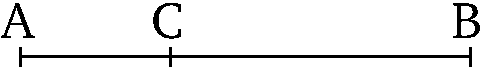
\includegraphics{Book10/fig073e.pdf}}

For let the straight-line $BC$, which is incommensurable in
square with $AB$, and fulfils the (other) prescribed (conditions), be
subtracted from the straight-line $AB$ [Prop.~10.34]. I say that the remainder
$AC$ is the aforementioned irrational (straight-line).

For since the sum of the squares on $AB$ and $BC$ is medial, and
twice the (rectangle contained) by $AB$ and $BC$ rational,
the (sum of the squares) on $AB$ and $BC$ is thus incommensurable
with twice the (rectangle contained) by $AB$ and $BC$. Thus, the
remaining (square) on $AC$ is also incommensurable with
twice the (rectangle contained) by $AB$ and $BC$ [Props.~2.7, 10.16]. And twice
the (rectangle contained) by $AB$ and $BC$ is rational. 
Thus, the (square) on $AC$ is irrational. Thus, $AC$ is an
irrational (straight-line) [Def.~10.4]. And let it be
called that which makes
with a rational (area) a medial whole.$^\dag$ (Which is) the very thing it
was required to show.}
\end{Parallel}
{\footnotesize\noindent$^\dag$ See footnote to Prop.~10.40.}

%%%%
%10.78
%%%%
\pdfbookmark[1]{Proposition 10.78}{pdf10.78}
\begin{Parallel}{}{}
\ParallelLText{
\begin{center}
{\large \ggn{78}.}
\end{center}\vspace*{-7pt}

\gr{Ἐὰν ἀπὸ εὐθείαξ εὐθεῖα ἀφαιρεθῆ| δυνάμει ἀσύμμ\-ετροξ
ο>ῦσα τῆ| <όλῃ, μετὰ δὲ τῆξ <όληξ ποιοῦσα τό τε συγκείμενον
ἐκ τῶν ἀπ> α\kern -.7pt  ὐτῶν τετραγώνων μέσον τό τε δὶξ ὑπ> α\kern -.7pt  ὐτῶν
μέσον καὶ >έτι τὰ ἀπ> α\kern -.5pt  ὐτῶν τετράγωνα ἀσύμμετρα τῶ|
δὶξ ὑπ> α\kern -.3pt  ὐτῶν, ἡ λοιπὴ >άλογόξ ἐστιν; καλείσθω δὲ ἡ μετὰ
μέσου μέσον τὸ <όλον ποιοῦσα.}\\~\\

% Removed epsf size command
\centerline{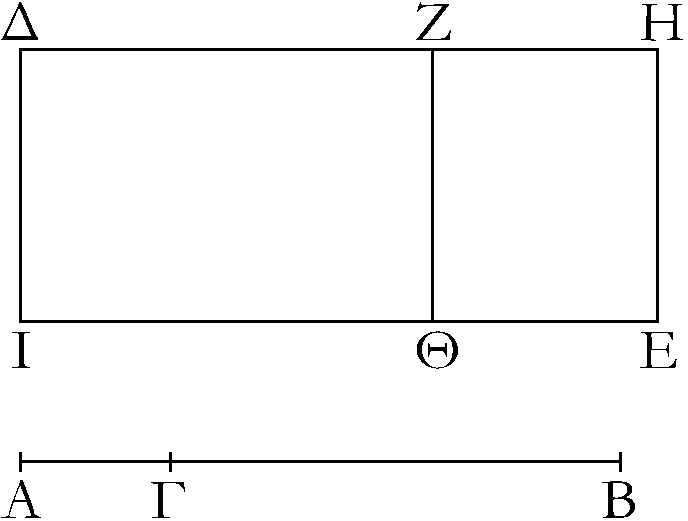
\includegraphics{Book10/fig078g.pdf}}

\gr{Ἀπὸ γὰρ εὐθείαξ τῆξ ΑΒ εὐθεῖα ἀφῃρήσθω ἡ ΒΓ δυνάμει
ἀσύμμετροξ ο>ῦσα τῆ| ΑΒ ποιοῦσα τὰ προκείμενα; λέγω,
<ότι ἡ λοιπὴ ἡ ΑΓ >άλογόξ ἐστιν ἡ καλουμένη ἡ μετὰ
μέσου μέσον τὸ <όλον ποιοῦσα.}

\gr{Ἐκκείσθω γὰρ <ρητὴ ἡ ΔΙ, καὶ τοῖξ μὲν ἀπὸ τῶν ΑΒ, ΒΓ >ίσον
παρὰ τὴν ΔΙ παραβεβλήσθω τὸ ΔΕ πλάτοξ ποιοῦν τὴν ΔΗ, τῶ| δὲ δὶξ
ὑπὸ τῶν ΑΒ, ΒΓ >ίσον ἀφῃρήσθω τὸ ΔΘ [πλάτοξ ποιοῦν τὴν
ΔΖ]. λοιπὸν >άρα τὸ ΖΕ >ίσον ἐστὶ τῶ| ἀπὸ τῆξ ΑΓ;
<ώστε ἡ ΑΓ δύναται τὸ ΖΕ. καὶ ἐπεὶ τὸ συγκείμενον ἐκ
τῶν ἀπὸ τῶν ΑΒ, ΒΓ τετραγώνων μέσον ἐστὶ καί ἐστιν
>ίσον τῶ| ΔΕ, μέσον >άρα [ἐστὶ] τὸ ΔΕ. καὶ παρὰ <ρητὴν
τὴν ΔΙ παράκειται πλάτοξ ποιοῦν τὴν ΔΗ; <ρητὴ
>άρα ἐστὶν ἡ ΔΗ καὶ ἀσύμμετροξ τῆ| ΔΙ μ\kern -.7pt  ήκει. πάλιν,
ἐπεὶ τὸ δὶξ ὑπὸ τῶν ΑΒ, ΒΓ μέσον ἐστὶ καί ἐστιν >ίσον
τῶ| ΔΘ, τὸ >άρα ΔΘ μέσον ἐστίν. καὶ παρὰ <ρητὴν τὴν
ΔΙ παράκειται πλάτοξ ποιοῦν  τὴν ΔΖ;
<ρητὴ >άρα ἐστὶ καὶ ἡ ΔΖ καὶ ἀσύμμετροξ τῆ| ΔΙ μ\kern -.7pt  ήκει.
 καὶ ἐπεὶ ἀσύμμετρά ἐστι τὰ ἀπὸ τῶν
ΑΒ, ΒΓ τῶ| δὶξ ὑπὸ τῶν ΑΒ, ΒΓ, ἀσύμμετρον >άρα καὶ
τὸ ΔΕ τῶ| ΔΘ. ὡξ δὲ τὸ ΔΕ πρὸξ τὸ ΔΘ, ο<ύτωξ ἐστὶ
καὶ ἡ ΔΗ πρὸξ τὴν ΔΖ; ἀσύμμετροξ >άρα ἡ ΔΗ τῆ| ΔΖ.
καί εἰσιν ἀμφότεραι <ρηταί; αἱ ΗΔ, ΔΖ >άρα <ρηταί
εἰσι δυνάμει μόνον σύμμετροι. ἀποτομ\kern -.5pt  ὴ >άρα ἐστίν ἡ
ΖΗ; <ρητὴ δὲ ἡ ΖΘ. τὸ δὲ ὑπὸ <ρητῆξ καὶ ἀποτομ\kern -.3pt  ῆξ
περιεχόμενον [ὀρθογώνιον] >άλογόν ἐστιν, καὶ ἡ δυναμένη
α\kern -.7pt  ὐτὸ >άλογόξ ἐστιν; καὶ δύναται τὸ ΖΕ ἡ ΑΓ; ἡ ΑΓ >άρα >άλογόξ ἐστιν;
 καλείσθω δὲ ἡ μετὰ μέσου μέσον τὸ <όλον
ποιοῦσα. <όπερ >έδει δεῖχαι.}}

\ParallelRText{
\begin{center}
{\large Proposition 78}
\end{center}

If a straight-line, which is incommensurable in square with the whole, and with the whole
makes the sum of the squares on them medial, and twice the (rectangle
contained) by them medial, and, moreover, the (sum of the) squares on them
incommensurable with twice the (rectangle contained) by them, is
subtracted from a(nother) straight-line  then the
remainder is an irrational (straight-line). Let it be called that which makes
with a medial (area) a medial whole.

% Removed epsf size command
\centerline{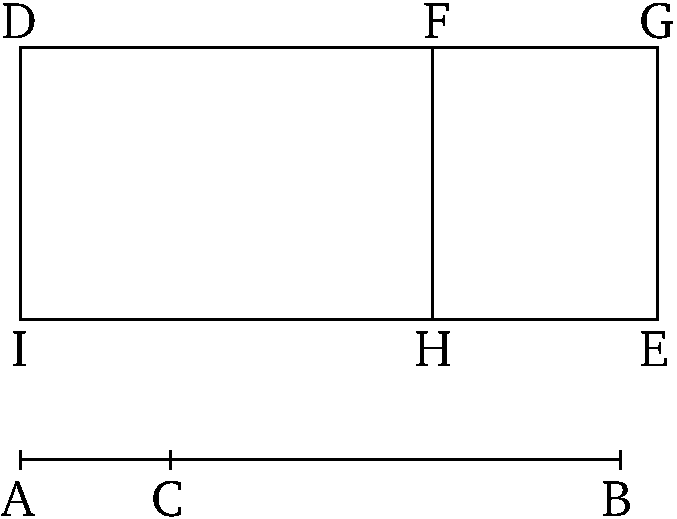
\includegraphics{Book10/fig078e.pdf}}

For let the straight-line $BC$, which is incommensurable in square
$AB$, and fulfils the (other) prescribed (conditions), be subtracted from the
(straight-line) $AB$ [Prop.~10.35].  I say that the remainder $AC$ is the irrational (straight-line) called  that which makes with a medial (area) a medial whole.

For let the rational (straight-line) $DI$ be laid down. And let $DE$, equal to
the (sum of the squares) on $AB$ and $BC$, be applied to $DI$,
producing $DG$ as breadth. And let $DH$, equal to twice the (rectangle
contained) by $AB$ and $BC$, be subtracted (from $DE$) [producing
$DF$ as breadth]. Thus, the remainder $FE$ is equal to the (square) on 
$AC$ [Prop.~2.7]. Hence, $AC$ is the square-root of $FE$. And since the sum of the squares on $AB$ and $BC$ is medial, and
is equal to $DE$, $DE$ [is] thus medial. And it is applied to the
rational (straight-line) $DI$, producing $DG$ as breadth. Thus, $DG$
is rational, and incommensurable in length with $DI$ [Prop~10.22]. Again, since twice the (rectangle
contained) by $AB$ and $BC$ is medial, and is equal to $DH$, $DH$
is thus medial. And it is applied to the rational (straight-line)
$DI$, producing $DF$ as breadth.  Thus, $DF$ is also rational, and incommensurable in length with $DI$ [Prop.~10.22]. And since  the (sum of the squares)
on $AB$ and $BC$ is incommensurable with twice the (rectangle contained)
by $AB$ and $BC$, $DE$ (is) also incommensurable with $DH$. 
And as $DE$ (is) to $DH$, so $DG$  also is to $DF$ [Prop.~6.1]. Thus, $DG$ (is) incommensurable (in length) with
$DF$ [Prop.~10.11]. And they are both rational. 
Thus, $GD$ and $DF$ are rational (straight-lines which are) commensurable
in square only. Thus, $FG$ is an apotome [Prop.~10.73]. And $FH$ (is) rational. And the
[rectangle] contained by a rational (straight-line) and an apotome is
irrational [Prop.~10.20], and its square-root
is irrational. And $AC$ is the square-root of $FE$.  Thus, $AC$
is irrational. Let it be called that which makes with a medial (area) a medial
whole.$^\dag$ 
(Which is) the very thing it was required to show.}
\end{Parallel}
{\footnotesize\noindent$^\dag$ See footnote to Prop.~10.41.}

%%%%
%10.79
%%%%
\pdfbookmark[1]{Proposition 10.79}{pdf10.79}
\begin{Parallel}{}{}
\ParallelLText{
\begin{center}
{\large \ggn{79}.}
\end{center}\vspace*{-7pt}

\gr{Τῆ| ἀποτομ\kern -.7pt  ῆ| μία [μόνον] προσαρμόζει εὐθεῖα <ρητὴ δυνάμει
μόνον σύμμετροξ ο>ῦσα τῆ| <όλῃ.}\\

% Removed epsf size command
\centerline{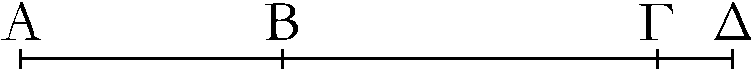
\includegraphics{Book10/fig079g.pdf}}

\gr{>'Εστω ἀποτομ\kern -.7pt  ὴ ἡ ΑΒ, προσαρμόζουσα δὲ α\kern -.7pt  ὐτῆ| ἡ ΒΓ; αἱ ΑΓ, ΓΒ
>άρα <ρηταί εἰσι δυνάμει μόνον σύμμετροι; λέγω, <ότι τῆ| ΑΒ ἑτέρα οὐ
προσαρμόζει <ρητὴ δυνάμει μόνον σύμμετροξ ο>ῦσα τῆ| <όλῆ|.}

\gr{Εἰ γὰρ δυνατόν, προσαρμοζέτω ἡ ΒΔ; καὶ αἱ ΑΔ, ΔΒ >άρα <ρηταί
εἰσι δυνάμει μόνον σύμμετροι. καὶ ἐπεί, <ῶ| ὑπερέθει τὰ
ἀπὸ τῶν ΑΔ, ΔΒ τοῦ δὶξ ὑπὸ τῶν ΑΔ, ΔΒ, τούτῳ ὑπερέθει
καὶ τὰ ἀπὸ τῶν ΑΓ, ΓΒ τοῦ δὶξ ὑπὸ τῶν ΑΓ, ΓΒ; τῶ| γὰρ
α\kern -.7pt  ὐτῶ| τῶ| ἀπὸ τῆξ ΑΒ ἀμφότερα ὑπερέθει; ἐναλλὰχ >άρα, <ῶ|
ὑπερέθει τὰ ἀπὸ τῶν ΑΔ, ΔΒ τῶν ἀπὸ τῶν ΑΓ, ΓΒ, τούτῳ ὑπερέθει [καὶ] τὸ δὶξ ὑπὸ τῶν ΑΔ, ΔΒ
τοῦ δὶξ ὑπὸ τῶν ΑΓ, ΓΒ. τὰ δὲ ἀπὸ τῶν ΑΔ, ΔΒ τῶν ἀπὸ τῶν
ΑΓ, ΓΒ ὑπερέθει <ρητῶ|; <ρητὰ γὰρ ἀμφότερα. καὶ τὸ δὶξ >άρα ὑπὸ
τῶν ΑΔ, ΔΒ τοῦ δὶξ ὑπὸ τῶν ΑΓ, ΓΒ ὑπερέθει <ρητῶ|; <όπερ ἐστὶν ἀδύνατον; μέσα γὰρ ἀμφότερα, μέσον δὲ μέσου οὐθ ὑπερέθει
<ρητῶ|. τῆ| >άρα ΑΒ ἑτέρα οὐ προσαρμόζει <ρητὴ δυνάμει
μόνον σύμμετροξ ο>ῦσα τῆ| <όλῃ.}

\gr{Μία >άρα μόνη τῆ| ἀποτομ\kern -.7pt  ῆ| προσαρμόζει <ρητὴ δυνάμει
μόνον σύμμετροξ ο>ῦσα τῆ| <όλῃ; <όπερ >έδει
δεῖχαι.}}

\ParallelRText{
\begin{center}
{\large Proposition 79}
\end{center}

\mbox{[}Only] one rational straight-line, which is
commensurable in square only with the whole, can be attached to an apotome.$^\dag$

% Removed epsf size command
\centerline{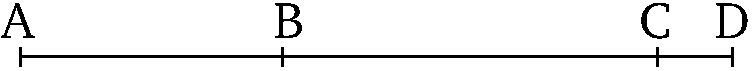
\includegraphics{Book10/fig079e.pdf}}

Let $AB$ be an apotome, with $BC$  (so) attached to it. $AC$ and $CB$ are thus
rational (straight-lines which are) commensurable in square only [Prop.~10.73]. I say that another rational (straight-line), which is commensurable in  square only with the whole, cannot
be attached to $AB$. 

For, if possible, let $BD$ be (so) attached (to $AB$). Thus, $AD$ and $DB$ are also
rational (straight-lines which are) commensurable in square only [Prop.~10.73]. And since by whatever (area)
the (sum of the squares) on $AD$ and $DB$ exceeds twice the
(rectangle contained) by $AD$ and $DB$, the (sum of the squares)
on $AC$ and $CB$ also exceeds twice the (rectangle contained) by $AC$ and
$CB$ by this (same area). For both exceed by the same (area)---(namely), the (square)
on $AB$ [Prop.~2.7]. Thus, alternately, 
by whatever (area) the (sum of the squares) on $AD$ and 
$DB$ exceeds the (sum of the squares) on $AC$ and $CB$, 
 twice the (rectangle contained) by $AD$ and $DB$
[also] exceeds twice the (rectangle contained) by $AC$ and $CB$ by this (same area).
And the (sum of the squares) on $AD$ and $DB$ exceeds the (sum
of the squares) on $AC$ and $CB$ by a rational (area). For both
(are) rational (areas). Thus, twice the (rectangle contained) by $AD$ and $DB$ also
exceeds twice the (rectangle contained) by $AC$ and $CB$ by a
rational (area). The very thing is impossible. For both are
medial (areas) [Prop.~10.21],
and a medial (area) cannot exceed a(nother) medial (area) by a rational
(area) [Prop.~10.26].  
Thus, another rational (straight-line), which is commensurable in  square only with the whole, cannot
be attached to $AB$.

Thus, only one rational (straight-line), which is
commensurable in square only with the whole, can be attached to an apotome.
(Which is) the very thing it was required to show.}
\end{Parallel}
{\footnotesize\noindent$^\dag$ This proposition is equivalent to 
Prop.~10.42, with minus signs instead of
plus signs.}

%%%%
%10.80
%%%%
\pdfbookmark[1]{Proposition 10.80}{pdf10.80}
\begin{Parallel}{}{}
\ParallelLText{
\begin{center}
{\large \ggn{80}.}
\end{center}\vspace*{-7pt}

\gr{Τῆ| μέσηξ ἀποτομ\kern -.7pt  ῆ| πρώτῃ μία μόνον προσαρμόζει εὐθεῖα
μέση δυνάμει μόνον σύμμετροξ ο>ῦσα τῆ| <όλῃ, μετὰ δὲ τῆξ <όληξ
<ρητὸν περιέθουσα.}\\

% Removed epsf size command
\centerline{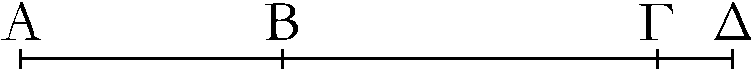
\includegraphics{Book10/fig079g.pdf}}

\gr{>'Εστω γὰρ μέσηξ ἀποτομ\kern -.7pt  ὴ πρώτη ἡ ΑΒ, καὶ τῆ| ΑΒ προσαρμοζέτω ἡ ΒΓ; αἱ ΑΓ,
ΓΒ >άρα μέσαι εἰσὶ δυνάμει μόνον σύμμετροι <ρητὸν περιέθουσαι
τὸ ὑπὸ τῶν ΑΓ, ΓΒ; λέγω, <ότι τῆ| ΑΒ ἑτέρα οὐ προσαρμόζει
μέση δυνάμει μόνον σύμμετροξ ο>ῦσα τῆ| <όλῃ, μετὰ δὲ
τῆξ <όληξ <ρητὸν περιέθουσα.}

\gr{Εἰ γὰρ δυνατόν, προσαρμοζέτω καὶ ἡ ΔΒ; αἱ >άρα 
ΑΔ, ΔΒ μέσαι εἰσὶ δυνάμει μόνον σύμμετροι <ρητὸν περιέθουσαι
τὸ ὑπὸ τῶν ΑΔ, ΔΒ. καὶ ἐπεί, <ῶ| ὑπερέθει τὰ ἀπὸ τῶν
ΑΔ, ΔΒ τοῦ δὶξ ὑπὸ τῶν ΑΔ, ΔΒ, τούτῳ ὑπερέθει καὶ τὰ ἀπὸ
τῶν ΑΓ, ΓΒ τοῦ δὶξ ὑπὸ τῶν ΑΓ, ΓΒ; τῶ| γὰρ α\kern -.7pt  ὐτῶ| [πάλιν]
ὑπερέθουσι τῶ| ἀπὸ τῆξ ΑΒ; ἐναλλὰχ >άρα, <ῶ| ὑπερέθει τὰ
ἀπὸ τῶν ΑΔ, ΔΒ τῶν ἀπὸ τῶν ΑΓ, ΓΒ, τούτῳ ὑπερέθει
καὶ τὸ δὶξ ὑπὸ τῶν
ΑΔ, ΔΒ τοῦ δὶξ ὑπὸ τῶν
ΑΓ, ΓΒ. τὸ δὲ δὶξ ὑπὸ τῶν ΑΔ, ΔΒ τοῦ δὶξ ὑπὸ τῶν ΑΓ, ΓΒ
ὑπερέθει <ρητῶ|; <ρητὰ γὰρ ἀμφότερα. καὶ τὰ ἀπὸ τῶν ΑΔ, ΔΒ
>άρα τῶν ἀπὸ τῶν ΑΓ, ΓΒ [τετραγώνων]
ὑπερέθει <ρητῶ|; <όπερ ἐστὶν ἀδύνατον; μέσα γάρ ἐστιν ἀμφότερα,
μέσον δὲ μέσου οὐθ ὑπερέθει <ρητῶ|.}

\gr{Τῆ| >άρα μέσηξ ἀποτομ\kern -.7pt  ῆ| πρώτῃ μία μόνον προσαρμόζει
εὐθεῖα μέση δυνάμει μόνον σύμμετροξ ο>ῦσα τῆ| <όλῃ,
μετὰ δὲ τῆξ <όληξ <ρητὸν περιέθουσα; <όπερ >έδει δεῖχαι.}}

\ParallelRText{
\begin{center}
{\large Proposition 80}
\end{center}

Only one medial straight-line,
which is commensurable in square only with the whole, and
contains a rational (area) with the whole, can be attached
to a first apotome of a medial (straight-line).$^\dag$

% Removed epsf size command
\centerline{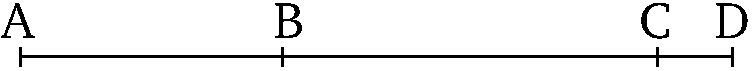
\includegraphics{Book10/fig079e.pdf}}

For let $AB$ be a first apotome of a medial (straight-line), and let $BC$ be (so) attached
to $AB$. Thus, $AC$ and $CB$ are medial (straight-lines which are)
commensurable in square only, containing a rational (area)---(namely, that
contained) by $AC$ and $CB$ [Prop.~10.74]. 
I say that a(nother) medial (straight-line), which is commensurable in square only with the whole, and
contains a rational (area) with the whole, cannot be attached to $AB$.

For, if possible, let $DB$ also be (so) attached to $AB$. Thus, $AD$ and
$DB$ are medial (straight-lines which are) commensurable in square only, containing a rational (area)---(namely, that)
contained by $AD$ and $DB$ [Prop.~10.74]. 
And since by whatever (area)
the (sum of the squares) on $AD$ and $DB$ exceeds twice the
(rectangle contained) by $AD$ and $DB$,  the (sum of the squares)
on $AC$ and $CB$ also exceeds twice the (rectangle contained) by $AC$ and
$CB$ by this (same area). For [again] both exceed by the same (area)---(namely), the (square)
on $AB$ [Prop.~2.7]. Thus, alternately, 
by whatever (area) the (sum of the squares) on $AD$ and 
$DB$ exceeds the (sum of the squares) on $AC$ and $CB$, 
 twice the (rectangle contained) by $AD$ and $DB$
also exceeds twice the (rectangle contained) by $AC$ and $CB$ by this (same area).
And twice the (rectangle contained) by $AD$ and $DB$ exceeds twice the (rectangle contained) by $AC$ and $CB$ by a rational (area). For both
(are) rational (areas). Thus,  the (sum of the squares) on $AD$ and $DB$ also
exceeds the (sum of the) [squares] on $AC$ and $CB$ by a
rational (area). The very thing is impossible. For both are
medial (areas) [Props.~10.15, 10.23~corr.],
and a medial (area) cannot exceed a(nother) medial (area) by a rational
(area) [Prop.~10.26].

Thus, only one medial (straight-line),
which is commensurable in square only with the whole, and
contains a rational (area) with the whole, can be attached
to a first apotome of a medial (straight-line). (Which is) the very thing it was required to
show.}
\end{Parallel}
{\footnotesize\noindent$^\dag$ This proposition is equivalent to 
Prop.~10.43, with minus signs instead of
plus signs.}

%%%%
%10.81
%%%%
\pdfbookmark[1]{Proposition 10.81}{pdf10.81}
\begin{Parallel}{}{}
\ParallelLText{
\begin{center}
{\large \ggn{81}.}
\end{center}\vspace*{-7pt}

\gr{Τῆ| μέσηξ ἀποτομ\kern -.7pt  ῆ| δευτέρᾳ μία μόνον προσαρμόζει εὐθεῖα
μέση δυνάμει μόνον σύμμετροξ τῆ| <όλῃ, μετὰ δὲ τῆξ <όληξ
μέσον περιέθουσα.}\\

% Removed epsf size command
\centerline{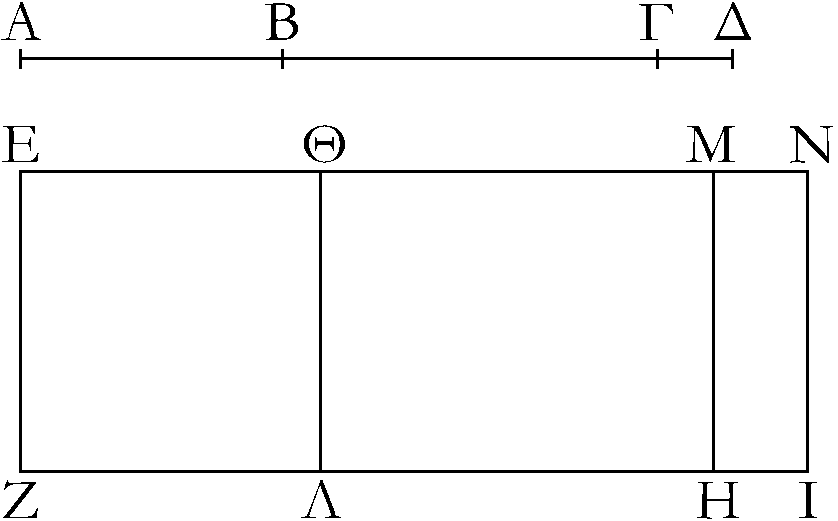
\includegraphics{Book10/fig081g.pdf}}

\gr{>'Εστω μέσηξ ἀποτομ\kern -.7pt  ὴ δευτέρα ἡ ΑΒ καὶ τῆ| ΑΒ προσαρμόζουσα
ἡ ΒΓ; αἱ >άρα ΑΓ, ΓΒ μέσαι εἰσὶ δυνάμει μόνον σύμμετροι
μέσον περιέθουσαι τὸ ὑπὸ τῶν ΑΓ, ΓΒ; λέγω, <ότι τῆ| ΑΒ
ἑτέρα οὐ προσαρμόσει εὐθεῖα μέση δυνάμει μόνον σύμμετροξ
ο>ῦσα τῆ| <όλῃ, μετὰ δὲ τῆξ <όληξ μέσον περιέθουσα.}

\gr{Εἰ γὰρ δυνατόν, προσαρμοζέτω ἡ ΒΔ; καὶ αἱ ΑΔ,
ΔΒ >άρα μέσαι εἰσὶ δυνάμει μόνον σύμμετροι μέσον περιέθουσαι
τὸ ὑπὸ τῶν ΑΔ, ΔΒ. καὶ ἐκκείσθω <ρητὴ ἡ ΕΖ, καὶ τοῖξ μὲν
ἀπὸ τῶν ΑΓ, ΓΒ >ίσον παρὰ τὴν ΕΖ παραβεβλήσθω τὸ ΕΗ πλάτοξ ποιοῦν
τὴν ΕΜ; τῶ| δὲ δὶξ ὑπὸ τῶν ΑΓ, ΓΒ >ίσον ἀφῃρήσθω τὸ ΘΗ
πλάτοξ ποιοῦν τὴν ΘΜ; λοιπὸν >άρα τὸ ΕΛ >ίσον ἐστὶ τῶ|
ἀπὸ τῆξ ΑΒ; <ώστε ἡ ΑΒ δύναται τὸ ΕΛ. πάλιν δὴ τοῖξ
ἀπὸ τῶν ΑΔ, ΔΒ >ίσον παρὰ τὴν ΕΖ παραβεβλήσθω τὸ ΕΙ πλάτοξ
ποιοῦν τὴν ΕΝ; >έστι δὲ καὶ τὸ ΕΛ >ίσον τῶ| ἀπὸ τῆξ ΑΒ
τετραγώνῳ; λοιπὸν >άρα τὸ ΘΙ >ίσον ἐστὶ τῶ| δὶξ ὑπὸ τῶν ΑΔ, ΔΒ.
καὶ ἐπεὶ μέσαι εἰσὶν αἱ ΑΓ, ΓΒ, μέσα >άρα ἐστὶ καὶ τὰ
ἀπὸ τῶν ΑΓ, ΓΒ. καί ἐστιν >ίσα τῶ| ΕΗ; μέσον >άρα καὶ τὸ
ΕΗ. καὶ παρὰ <ρητὴν τὴν ΕΖ παράκειται πλάτοξ ποιοῦν τὴν ΕΜ;
<ρητὴ >άρα ἐστὶν ἡ ΕΜ καὶ ἀσύμμετροξ τῆ| ΕΖ μ\kern -.7pt  ήκει. 
πάλιν,
ἐπεὶ μέσον ἐστὶ τὸ ὑπὸ τῶν ΑΓ, ΓΒ, καὶ τὸ δὶξ ὑπὸ τῶν
ΑΓ, ΓΒ μέσον ἐστίν. καί ἐστιν >ίσον τῶ| ΘΗ; καὶ τὸ ΘΗ >άρα
μέσον ἐστίν. καὶ παρὰ <ρητὴν τὴν ΕΖ παράκειται πλάτοξ ποιοῦν
τὴν ΘΜ; <ρητὴ >άρα ἐστὶ καὶ ἡ ΘΜ καὶ ἀσύμμετροξ τῆ| ΕΖ
μ\kern -.7pt  ήκει. 
καὶ ἐπεὶ αἱ ΑΓ, ΓΒ δυνάμει μόνον σύμμετροί εἰσιν,
ἀσύμμετροξ >άρα ἐστὶν ἡ ΑΓ τῆ| ΓΒ μ\kern -.5pt  ήκει. ὡξ δὲ ἡ ΑΓ πρὸξ
τὴν ΓΒ, ο<ύτωξ ἐστὶ τὸ ἀπὸ τῆξ ΑΓ πρὸξ τὸ ὑπὸ τῶν ΑΓ, ΓΒ;
ἀσύμμετρον >άρα ἐστὶ τὸ ἀπὸ τῆξ ΑΓ  τῶ| ὑπὸ
τῶν ΑΓ, ΓΒ. ἀλλὰ τῶ| μὲν ἀπὸ τῆξ ΑΓ
σύμμετρά ἐστι τὰ ἀπὸ
τῶν ΑΓ, ΓΒ, τῶ| δὲ ὑπὸ τῶν ΑΓ, ΓΒ σύμμετρόν ἐστι τὸ δὶξ
ὑπὸ τῶν ΑΓ, ΓΒ; ἀσύμμετρα >άρα ἐστὶ τὰ ἀπὸ τῶν ΑΓ, ΓΒ
τῶ| δὶξ ὑπὸ τῶν ΑΓ, ΓΒ. καί ἐστι τοῖξ μὲν ἀπὸ τῶν
ΑΓ, ΓΒ >ίσον τὸ ΕΗ, τῶ| δὲ δὶξ ὑπὸ τῶν ΑΓ, ΓΒ >ίσον τὸ ΗΘ;
 ἀσύμμετρον >άρα ἐστὶ τὸ ΕΗ τῶ| ΘΗ.
ὡξ δὲ τὸ ΕΗ
πρὸξ τὸ ΘΗ, ο<ύτωξ ἐστὶν ἡ ΕΜ πρὸξ τὴν ΘΜ; 
ἀσύμμετροξ
>άρα ἐστὶν ἡ ΕΜ τῆ| ΜΘ μ\kern -.3pt  ήκει. καί εἰσιν ἀμφότεραι <ρηταί;
αἱ ΕΜ, ΜΘ >άρα <ρηταί εἰσι δυνάμει μόνον σύμμετροι;
ἀποτομ\kern -.7pt  ὴ >άρα ἐστὶν ἡ ΕΘ, προσαρμόζουσα δὲ α\kern -.7pt  ὐτῆ| 
ἡ ΘΜ. ὁμοίωξ δὴ δείχομεν, <ότι καὶ ἡ ΘΝ α\kern -.7pt  ὐτῆ| 
προσαρμόζει;
τῆ| >άρα ἀποτομ\kern -.7pt  ῆ| >άλλη καὶ >άλλη προσαρμόζει εὐθεῖα δυνάμει
μόνον σύμμετροξ ο>ῦσα τῆ| <όλῃ; <όπερ ἐστὶν ἀδύνατον.}

\gr{Τῆ| >άρα μέσηξ ἀποτομ\kern -.7pt  ῆ| δευτέρᾳ μία μόνον προσαρμόζει εὐθεῖα
μέση δυνάμει μόνον σύμμετροξ ο>ῦσα τῆ| <όλῃ, μετὰ δὲ τῆξ
<όληξ μέσον περιέθουσα; <όπερ >έδει δεῖχαι.}}

\ParallelRText{
\begin{center}
{\large Proposition 81}
\end{center}

Only one medial straight-line,
which is commensurable in square only with the whole, and
contains a medial (area) with the whole, can be attached
to a second apotome of a medial (straight-line).$^\dag$

% Removed epsf size command
\centerline{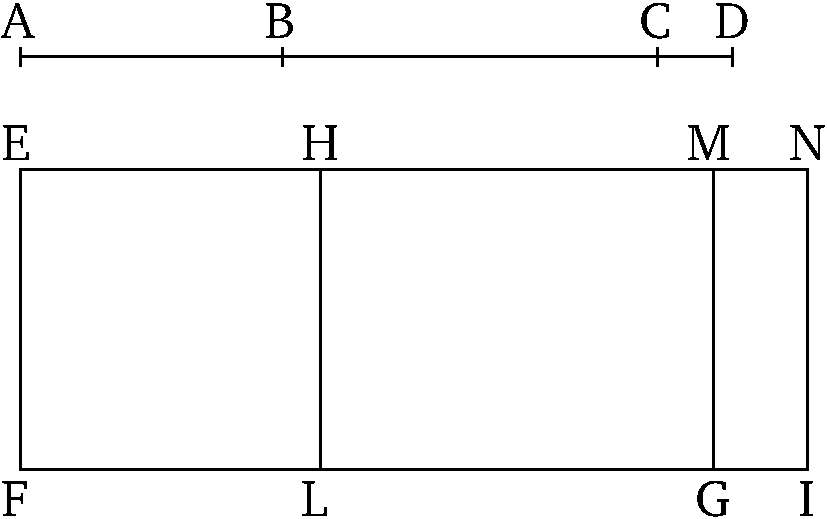
\includegraphics{Book10/fig081e.pdf}}

Let $AB$ be a second apotome of a medial (straight-line), with $BC$ (so) attached
to $AB$. Thus, $AC$ and $CB$ are medial (straight-lines which
are) commensurable in square only, containing a medial (area)---(namely,
that contained) by $AC$ and $CB$ [Prop.~10.75].
I say that a(nother) medial straight-line, which is commensurable in square
only with the whole, and contains a medial (area) with the whole, cannot
be attached to $AB$.

For, if possible, let $BD$ be (so) attached. Thus, $AD$ and $DB$ are also medial (straight-lines which
are) commensurable in square only, containing a medial (area)---(namely,
that contained) by $AD$ and $DB$ [Prop.~10.75].
And let the rational (straight-line) $EF$ be laid down. And let $EG$,
equal to the (sum of the squares) on $AC$ and $CB$, be applied
to $EF$, producing $EM$ as breadth. And let $HG$, equal to twice
the (rectangle contained) by $AC$ and $CB$, be subtracted
(from $EG$), producing $HM$ as breadth. The remainder $EL$ is
thus equal to the (square) on $AB$ [Prop.~2.7]. 
Hence, $AB$ is the square-root of $EL$. So, again, let $EI$, equal to
the (sum of the squares) on $AD$ and $DB$ be applied to $EF$,
producing $EN$ as breadth. And $EL$ is also equal to the square
on $AB$. Thus, the remainder 
$HI$ is equal to twice the (rectangle contained) by $AD$ and $DB$ [Prop.~2.7]. And since $AC$ and $CB$ are
(both) medial (straight-lines), the (sum of the squares) on $AC$ and $CB$ is also medial.
And it is equal to $EG$. Thus, $EG$ is also medial [Props.~10.15, 10.23~corr.]. And it is
applied to the rational (straight-line) $EF$, producing $EM$ as breadth.
Thus, $EM$ is rational, and incommensurable in length with $EF$
[Prop.~10.22]. Again, since the (rectangle
contained) by $AC$ and $CB$ is medial, twice the (rectangle
contained) by $AC$ and $CB$ is also medial [Prop.~10.23~corr.]. And it is equal to $HG$.
Thus, $HG$ is also medial. And it is applied to the rational (straight-line)
$EF$, producing $HM$ as breadth. Thus, $HM$ is also rational, and
incommensurable in length with $EF$ [Prop.~10.22]. And since $AC$ and $CB$ are commensurable in square only, $AC$ is thus incommensurable in length with $CB$.  And as $AC$ (is)
to $CB$, so the (square) on $AC$
is to the (rectangle contained) by $AC$ and $CB$ [Prop.~10.21~corr.]. Thus, the (square) on $AC$
is incommensurable with the (rectangle contained) by $AC$ and $CB$
[Prop.~10.11].
But, the (sum of the squares) on $AC$ and $CB$ is commensurable
with the (square) on $AC$, and twice the (rectangle contained) by $AC$ and
$CB$ is commensurable with the (rectangle contained) by $AC$ and $CB$ [Prop.~10.6].
Thus, the (sum of the squares) on $AC$ and $CB$ is incommensurable
with twice the (rectangle contained) by $AC$ and $CB$ [Prop.~10.13]. And $EG$ is equal to
the (sum of the squares) on $AC$ and $CB$. And $GH$ is equal
to twice the (rectangle contained) by $AC$ and $CB$. Thus, 
$EG$ is incommensurable with $HG$. And as $EG$ (is) to $HG$,
so $EM$ is to $HM$ [Prop.~6.1]. 
Thus, $EM$ is incommensurable in length with $MH $ [Prop.~10.11]. And they are both rational (straight-lines).
Thus, $EM$ and $MH $ are rational (straight-lines which are)
commensurable in square only. Thus, $EH$ is an apotome
[Prop.~10.73], and $HM$ (is) attached to
it. So, similarly, we can show that $HN$ (is) also (commensurable
in square only with $EN$ and is) attached to ($EH$). 
Thus, different straight-lines, which are commensurable
in square only with the whole, are attached to an apotome.
The very thing is impossible [Prop.~10.79].

Thus, only one medial straight-line,
which is commensurable in square only with the whole, and
contains a medial (area) with the whole, can be attached
to a second apotome of a medial (straight-line). (Which is) the very thing it was required to show.}
\end{Parallel}
{\footnotesize\noindent$^\dag$ This proposition is equivalent to 
Prop.~10.44, with minus signs instead of
plus signs.}

%%%%
%10.82
%%%%
\pdfbookmark[1]{Proposition 10.82}{pdf10.82}
\begin{Parallel}{}{}
\ParallelLText{
\begin{center}
{\large \ggn{82}.}
\end{center}\vspace*{-7pt}

\gr{Τῆ| ἐλάσσονι μία μόνον προσαρμόζει εὐθεῖα δυνάμει
ἀσύμμετροξ ο>ῦσα τῆ| <όλῃ ποιοῦσα μετὰ τῆξ <όληξ
τὸ μὲν ἐκ τῶν ἀπ> α\kern -.7pt  ὐτῶν τετραγώνων <ρητόν,
τὸ δὲ δὶξ ὑπ> α\kern -.7pt  ὐτῶν μέσον.}\\

% Removed epsf size command
\centerline{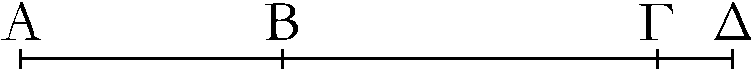
\includegraphics{Book10/fig079g.pdf}}

\gr{>'Εστω ἡ ἐλάσσων ἡ ΑΒ, καὶ τῆ| ΑΒ προσαρμόζουσα >έστω
ἡ ΒΓ; αἱ >άρα ΑΓ, ΓΒ δυνάμει εἰσὶν ἀσύμμετροι
ποιοῦσαι τὸ μὲν συγκείμενον ἐκ τῶν ἀπ> α\kern -.7pt  ὐτῶν τετραγώνων
<ρητόν, τὸ δὲ δὶξ ὑπ> α\kern -.7pt  ὐτῶν μέσον; λέγω, <ότι
τῆ| ΑΒ ἑτέρα εὐθεῖα οὐ προσαρμόσει τὰ α\kern -.5pt  ὐτὰ ποιοῦσα.}

\gr{Εἰ γὰρ δυνατόν, προσαρμοζέτω ἡ ΒΔ; καὶ αἱ ΑΔ,
ΔΒ >άρα δυνάμει εἰσὶν ἀσύμμετροι ποιοῦσαι τὰ προειρημένα.
καὶ ἐπεί, <ῶ| ὑπερέθει τὰ ἀπὸ τῶν ΑΔ, ΔΒ
τῶν ἀπὸ τῶν ΑΓ, ΓΒ, τούτῳ ὑπερέθει καὶ τὸ δὶξ
ὑπὸ τῶν ΑΔ, ΔΒ τοῦ δὶξ ὑπὸ τῶν ΑΓ, ΓΒ, τὰ δὲ
ἀπὸ τῶν ΑΔ, ΔΒ τετράγωνα τῶν ἀπὸ τῶν ΑΓ, ΓΒ
 τετραγώνων ὑπερέθει
<ρητῶ|; <ρητὰ γάρ ἐστιν ἀμφότερα; καὶ τὸ δὶξ ὑπὸ τῶν ΑΔ, ΔΒ
>άρα τοῦ δὶξ ὑπὸ τῶν ΑΓ, ΓΒ ὑπερέθει <ρητῶ|; <όπερ
ἐστὶν ἀδύνατον; μέσα γάρ ἐστιν ἀμφότερα.}

\gr{Τῆ| >άρα ἐλάσσονι μία μόνον προσαρμόζει εὐθεῖα δυνάμει
ἀσύμμετροξ ο>ῦσα τῆ| <όλῃ καὶ ποιοῦσα τὰ μὲν ἀπ> 
α\kern -.7pt  ὐτῶν τετράγωνα <άμα <ρητόν, τὸ δὲ δὶξ ὑπ> α\kern -.7pt  ὐτῶν
μέσον; <όπερ >έδει δεῖχαι.}}

\ParallelRText{
\begin{center}
{\large Proposition 82}
\end{center}

Only one straight-line, which is incommensurable
in square with the whole, and (together) with the whole makes the (sum of the) squares on them
rational, and twice the (rectangle contained) by them medial, can be
attached to a minor (straight-line).

% Removed epsf size command
\centerline{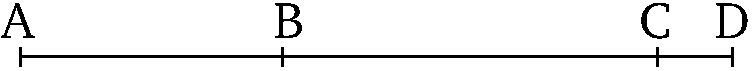
\includegraphics{Book10/fig079e.pdf}}

Let $AB$ be a minor (straight-line), and let $BC$ be (so) attached to $AB$.
Thus, $AC$ and $CB$ are (straight-lines which are) incommensurable  in square, making the sum of
the squares on them rational, and twice the (rectangle contained) by them
medial [Prop.~10.76]. I say that another
another straight-line fulfilling the same (conditions) cannot be
attached to $AB$.

For, if possible, let $BD$ be (so) attached (to $AB$). Thus, $AD$
and $DB$ are also (straight-lines which are) incommensurable in square, fulfilling the (other) aforementioned
(conditions) [Prop.~10.76]. And since
by whatever (area) the (sum of the squares) on $AD$ and $DB$
exceeds the (sum of the squares) on $AC$ and $CB$, 
twice the (rectangle contained) by $AD$ and $DB$ also exceeds
twice the (rectangle contained) by $AC$ and $CB$  by this (same area) [Prop.~2.7]. And the (sum of the) squares on
$AD$ and $DB$ exceeds the (sum of the) squares on $AC$ and $CB$
by a rational (area). For both are rational (areas). Thus, twice the
(rectangle contained) by $AD$ and $DB$ also exceeds
twice the (rectangle contained) by $AC$ and $CB$ by a rational (area).
The very thing is impossible. For both are medial (areas) [Prop.~10.26].

Thus,  only one straight-line, which is  incommensurable in square
with the whole, and (with the whole) makes the  squares on them
(added) together rational, and twice the (rectangle contained) by them medial, can be
attached to a minor (straight-line). (Which is) the very thing it was required to
show.}
\end{Parallel}
{\footnotesize\noindent$^\dag$ This proposition is equivalent to 
Prop.~10.45, with minus signs instead of plus signs.}

%%%%
%10.83
%%%%
\pdfbookmark[1]{Proposition 10.83}{pdf10.83}
\begin{Parallel}{}{}
\ParallelLText{
\begin{center}
{\large \ggn{83}.}
\end{center}\vspace*{-7pt}

\gr{Τῆ| μετὰ <ρητοῦ μέσον τὸ <όλον ποιούσῃ μία μόνον προσαρμόζει
εὐθεῖα δυνάμει ἀσύμμετροξ ο>ῦσα τῆ| <όλῃ, μετὰ δὲ τῆξ
<όληξ ποιοῦσα τὸ μὲν συγκείμενον ἐκ τῶν ἀπ>
α\kern -.7pt  ὐτῶν τετραγώνων μέσον, τὸ δὲ δὶξ ὑπ> α\kern -.7pt  ὐτῶν <ρητόν.}\\~\\

% Removed epsf size command
\centerline{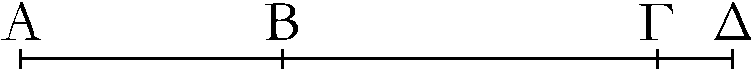
\includegraphics{Book10/fig079g.pdf}}

\gr{>'Εστω ἡ μετὰ <ρητοῦ μέσον τὸ <όλον ποιοῦσα ἡ ΑΒ,
καὶ τῆ| ΑΒ προσαρμοζέτω ἡ ΒΓ; αἱ >άρα ΑΓ, ΓΒ δυνάμει
εἰσὶν ἀσύμμετροι ποιοῦσαι τὰ προκείμενα; λέγω, <ότι
τῆ| ΑΒ ἑτέρα οὐ προσαρμόσει τὰ α\kern -.7pt  ὐτὰ ποιοῦσα.}

\gr{Εἰ γὰρ δυνατόν, προσαρμοζέτω ἡ ΒΔ; καὶ αἱ ΑΔ, ΔΒ >άρα
εὐθεῖαι δυνάμει εἰσὶν ἀσύμμετροι ποιοῦσαι τὰ
προκείμενα. ἐπεὶ οὐν, <ῶ| ὑπερέθει τὰ ἀπὸ τῶν
ΑΔ, ΔΒ τῶν ἀπὸ τῶν ΑΓ, ΓΒ, τούτῳ ὑπερέθει καὶ τὸ
δὶξ ὑπὸ τῶν ΑΔ, ΔΒ τοῦ δὶξ ὑπὸ τῶν ΑΓ, ΓΒ
ἀκολούθωξ τοῖξ πρὸ α\kern -.7pt  ὐτοῦ, τὸ δὲ δὶξ ὑπὸ τῶν ΑΔ, ΔΒ
τοῦ δὶξ ὑπὸ τῶν ΑΓ, ΓΒ ὑπερέθει <ρητῶ|; <ρητὰ γάρ
ἐστιν ἀμφότερα; καὶ τὰ ἀπὸ τῶν ΑΔ, ΔΒ >άρα τῶν
ἀπὸ τῶν ΑΓ, ΓΒ ὑπερέθει <ρητῶ|; <όπερ ἐστὶν
ἀδύνατον; μέσα γάρ ἐστιν ἀμφότερα.}

 \gr{Οὐκ >άρα τῆ| ΑΒ
ἑτέρα προσαρμόσει εὐθεῖα δυνάμει ἀσύμμετροξ ο>ῦσα τῆ|
<όλῃ, μετὰ δὲ τῆξ <όληξ ποιοῦσα τὰ προειρημένα;
μία >άρα μόνον προσαρμόσει; <όπερ >έδει δεῖχαι.}}

\ParallelRText{
\begin{center}
{\large Proposition 83}
\end{center}

Only  one straight-line, which is incommensurable
in square with the whole, and (together) with the whole makes the sum of the squares on them
medial, and twice the (rectangle contained) by them rational, can be
attached to that (straight-line) which with a rational (area) makes a
medial whole.$^\dag$

% Removed epsf size command
\centerline{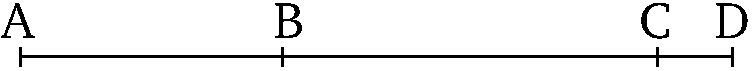
\includegraphics{Book10/fig079e.pdf}}

Let $AB$ be a (straight-line) which with a rational (area) makes a medial
whole,  and let $BC$ be (so) attached to $AB$. Thus, $AC$ and $CB$
are (straight-lines which are) incommensurable in square, fulfilling the (other) proscribed (conditions) [Prop.~10.77]. I say that another (straight-line)
fulfilling the same (conditions) cannot be attached to $AB$.

For, if possible, let $BD$ be (so) attached (to $AB$). Thus, $AD$ and
$DB$ are also straight-lines (which are) incommensurable in square,
fulfilling the (other) prescribed  (conditions) [Prop.~10.77]. Therefore, analogously to the
(propositions) before this, since by whatever (area)
the (sum of the squares) on $AD$ and $DB$ exceeds the (sum of the
squares) on $AC$ and $CB$,  twice the (rectangle contained)
by $AD$ and $DB$ also exceeds twice the (rectangle contained) by
$AC$ and $CB$ by this (same area). And twice the (rectangle contained) by $AD$ and
$DB$ exceeds twice the (rectangle contained) by $AC$ and
$CB$ by a rational (area). For they are (both) rational (areas).
Thus, the (sum of the squares) on 
$AD$ and $DB$ also exceeds the (sum of the squares) on $AC$ and $CB$
by a rational (area). The very thing is impossible. For both are
medial (areas) [Prop.~10.26].

 Thus, another
straight-line cannot be attached to $AB$, which is incommensurable
in square with the whole, and fulfills the (other) aforementioned (conditions) with the
whole. Thus, only one (such straight-line) can be (so) attached. (Which is)
the very thing it was required to show.}
\end{Parallel}
{\footnotesize\noindent$^\dag$
This proposition is equivalent to Prop.~10.46, with minus signs instead of
plus signs.}

%%%%
%10.84
%%%%
\pdfbookmark[1]{Proposition 10.84}{pdf10.84}
\begin{Parallel}{}{}
\ParallelLText{
\begin{center}
{\large \ggn{84}.}
\end{center}\vspace*{-7pt}

\gr{Τῆ| μετὰ μέσου μέσον τὸ <όλον ποιούσῃ μία μόνη προσαρμόζει εὐθεῖα δυνάμει ἀσύμμετροξ ο>ῦσα τῆ| <όλῃ, μετὰ δὲ τῆξ <όληξ ποιοῦσα τό τε συγκείμενον ἐκ τῶν ἀπ> α\kern -.7pt  ὐτῶν τετραγώνων
μέσον τό τε δὶξ ὑπ> α\kern -.7pt  ὐτῶν μέσον καὶ >έτι ἀσύμμετρον
τῶ| συγκειμένῳ ἐκ τῶν ἀπ> α\kern -.5pt  ὐτῶν.}

\gr{>'Εστω ἡ μετὰ μέσου μέσον τὸ <όλον ποιοῦσα ἡ ΑΒ,
προσαρμόζουσα δὲ α\kern -.7pt  ὐτῆ| ἡ ΒΓ; αἱ >άρα ΑΓ, ΓΒ δυνάμει εἰσὶν
ἀσύμμετροι ποιοῦσαι τὰ προειρημένα. λέγω, <ότι τῆ| ΑΒ ἑτέρα
οὐ προσαρμόσει ποιοῦσα προειρημένα.}\\~\\~\\~\\

% Removed epsf size command
\centerline{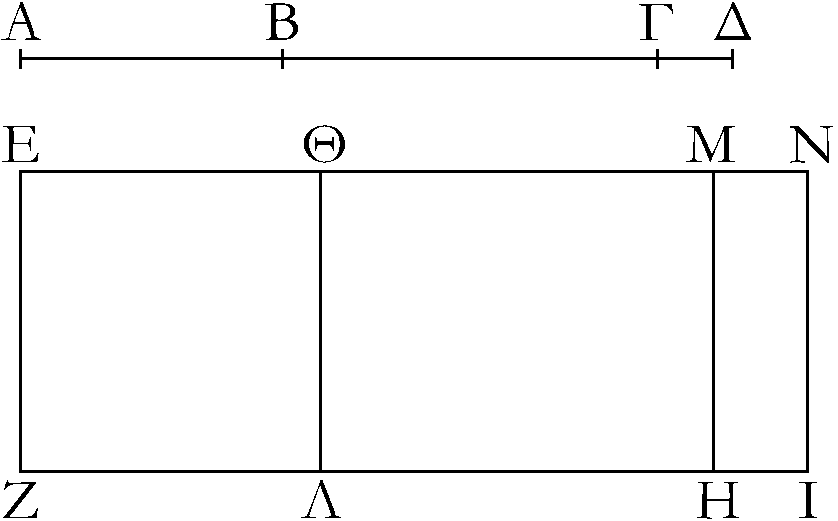
\includegraphics{Book10/fig081g.pdf}}

\gr{Εἰ γὰρ δυνατόν, προσαρμοζέτω ἡ ΒΔ, <ώστε καὶ τὰξ ΑΔ, ΔΒ δυνάμει
ἀσυμμέτρουξ ε>ῖναι ποιούσαξ τά τε ἀπὸ τῶν ΑΔ, ΔΒ τετράγωνα
<άμα μέσον καὶ τὸ δὶξ ὑπὸ τῶν ΑΔ, ΔΒ μέσον καὶ >έτι τὰ
ἀπὸ τῶν ΑΔ, ΔΒ ἀσύμμετρα τῶ| δὶξ ὑπὸ τῶν ΑΔ, ΔΒ; καὶ
ἐκκείσθω <ρητὴ ἡ ΕΖ, καὶ τοῖξ μὲν ἀπὸ τῶν ΑΓ, ΓΒ >ίσον
παρὰ τὴν ΕΖ παραβεβλήσθω τὸ ΕΗ πλάτοξ ποιοῦν τὴν ΕΜ, τῶ|
δὲ δὶξ ὑπὸ τῶν ΑΓ, ΓΒ >ίσον παρὰ τὴν ΕΖ παραβεβλήσθω τὸ ΘΗ
πλάτοξ ποιοῦν τὴν ΘΜ; λοιπὸν
>άρα τὸ ἀπὸ τῆξ ΑΒ >ίσον ἐστὶ τῶ| ΕΛ; ἡ >άρα ΑΒ δύναται
τὸ ΕΛ. πάλιν τοῖξ ἀπὸ τῶν ΑΔ, ΔΒ >ίσον
παρὰ τὴν ΕΖ παραβεβλήσθω τὸ ΕΙ πλάτοξ ποιοῦν τὴν ΕΝ.
 >έστι
δὲ καὶ τὸ ἀπὸ τῆξ ΑΒ >ίσον τῶ| ΕΛ;
λοιπὸν >άρα τὸ δὶξ ὑπὸ τῶν ΑΔ, ΔΒ >ίσον [ἐστὶ]
τῶ| ΘΙ. καὶ ἐπεὶ μέσον ἐστὶ τὸ συγκείμενον ἐκ τῶν
ἀπὸ τῶν ΑΓ, ΓΒ καί ἐστιν >ίσον τῶ| ΕΗ, μέσον >άρα ἐστὶ
καὶ τὸ ΕΗ. καὶ παρὰ <ρητὴν τὴν ΕΖ παράκειται πλάτοξ
ποιοῦν τὴν ΕΜ;
 <ρητὴ >άρα ἐστὶν ἡ ΕΜ καὶ ἀσύμμετροξ τῆ|
ΕΖ μ\kern -.7pt  ήκει. πάλιν, ἐπεὶ μέσον ἐστὶ τὸ δὶξ ὑπὸ τῶν ΑΓ, ΓΒ καί
ἐστιν >ίσον τῶ| ΘΗ, μέσον >άρα καὶ τὸ ΘΗ. καὶ παρὰ <ρητὴν τὴν
ΕΖ παράκειται πλάτοξ ποιοῦν τὴν ΘΜ; 
<ρητὴ >άρα ἐστὶν ἡ ΘΜ
καὶ ἀσύμμετροξ τῆ| ΕΖ μ\kern -.7pt  ήκει. καὶ ἐπεὶ ἀσύμμετρά ἐστι
τὰ ἀπὸ τῶν ΑΓ, ΓΒ τῶ| δὶξ ὑπὸ τῶν ΑΓ, ΓΒ, ἀσύμμετρόν
ἐστι καὶ τὸ ΕΗ τῶ| ΘΗ; ἀσύμμετροξ >άρα ἐστὶ καὶ ἡ ΕΜ τῆ|
ΜΘ μ\kern -.5pt  ήκει. καί εἰσιν ἀμφότεραι <ρηταί; αἱ >άρα ΕΜ, ΜΘ <ρηταί
εἰσι δυνάμει μόνον σύμμετροι; ἀποτομ\kern -.3pt  ὴ >άρα ἐστὶν ἡ ΕΘ, προσαρμόζουσα δὲ α\kern -.7pt  ὐτῆ| ἡ ΘΜ. ὁμοίωξ δὴ δείχομεν, <ότι ἡ ΕΘ πάλιν ἀποτομ\kern -.7pt  ή
ἐστιν, προσαρμόζουσα δὲ α\kern -.7pt  ὐτῆ| ἡ ΘΝ. τῆ| >άρα ἀποτομ\kern -.7pt  ῆ|
>άλλη καὶ >άλλη προσαρμόζει <ρητὴ δυνάμει μόνον σύμμετροξ
ο>ῦσα τῆ| <όλῃ; <όπερ ἐδείθθη ἀδύνατον. οὐκ >άρα τῆ| ΑΒ ἑτέρα
προσαρμόσει εὐθεῖα.}

\gr{Τῆ| >άρα ΑΒ μία μόνον προσαρμόζει εὐθεῖα δυνάμει
ἀσύμμετροξ ο>ῦσα τῆ| <όλῃ, μετὰ δὲ τῆξ <όληξ ποιοῦσα
τά τε ἀπ> α\kern -.7pt  ὐτῶν τετράγωνα <άμα μέσον καὶ τὸ δὶξ ὑπ>
α\kern -.7pt  ὐτῶν μέσον καὶ >έτι τὰ ἀπ> α\kern -.5pt  ὐτῶν τετράγωνα ἀσύμμετρα
τῶ| δὶξ ὑπ> α\kern -.3pt  ὐτῶν; <όπερ >έδει δεῖχαι.}}

\ParallelRText{
\begin{center}
{\large Proposition 84}
\end{center}

Only one straight-line, which is incommensurable
in square with the whole, and (together) with the whole makes the sum of the
squares on them medial, and twice the (rectangle contained) by
them medial, and, moreover, incommensurable with the sum of
the (squares) on them, can be attached to that (straight-line) which with
a medial (area) makes a medial whole.$^\dag$

Let $AB$ be a (straight-line) which with a medial (area) makes a medial
whole, $BC$ being (so) attached to it. Thus, $AC$ and $CB$ are incommensurable in square, fulfilling the (other) aforementioned (conditions)
[Prop.~10.78]. I say that a(nother) (straight-line)
fulfilling the aforementioned (conditions) cannot be attached to $AB$.

% Removed epsf size command
\centerline{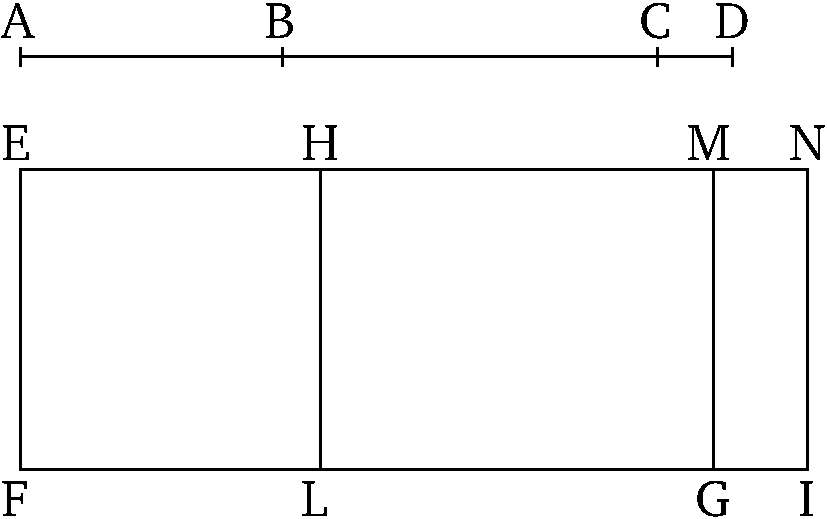
\includegraphics{Book10/fig081e.pdf}}

For, if possible, let $BD$ be (so) attached. Hence, $AD$ and
$DB$ are also (straight-lines which are) incommensurable in square, making the
squares on $AD$ and $DB$ (added) together medial, and twice the (rectangle contained) by $AD$ and $DB$ medial, and, moreover, the (sum of the squares)
on $AD$ and $DB$ incommensurable with twice the (rectangle contained)
by $AD$ and $DB$ [Prop.~10.78].
And let the rational (straight-line) $EF$ be laid down. And let $EG$, equal
to the (sum of the squares) on $AC$ and $CB$, be applied to
$EF$, producing $EM$ as breadth. And let $HG$, equal to twice the (rectangle contained) by $AC$ and $CB$, be applied to $EF$, producing $HM$ as breadth. Thus, the remaining (square) on  $AB$ is equal
to $EL$ [Prop.~2.7].  Thus, $AB$ is the square-root
of $EL$. Again, let $EI$, equal to the (sum of the squares) on $AD$ and $DB$, be applied to $EF$, producing $EN$ as breadth. And the (square) on $AB$
 is also equal to $EL$. Thus, the remaining twice the
(rectangle contained) by $AD$ and $DB$ [is] equal to $HI$ [Prop.~2.7].  And since the sum of the (squares) on $AC$ and $CB$ is medial, and is equal to $EG$, $EG$ is thus also medial.
And it is applied to the rational (straight-line) $EF$, producing $EM$ as breadth. $EM$ is thus rational, and incommensurable in length with $EF$
[Prop.~10.22]. Again, since twice the
(rectangle contained) by $AC$ and $CB$ is medial, and is equal to $HG$,
$HG$ is thus also medial. And it is applied to the rational (straight-line) $EF$,
producing $HM$ as breadth. $HM$ is thus rational, and incommensurable in
length with $EF$ [Prop.~10.22]. 
And since the (sum of the squares) on
 $AC$ and $CB$ is incommensurable
with twice the (rectangle contained) by $AC$ and $CB$, $EG$ is also incommensurable with $HG$. Thus, $EM$ is also incommensurable in length
with $MH $ [Props.~6.1, 10.11]. And they are both  rational (straight-lines). Thus, $EM$ and $MH $ are rational (straight-lines which are) commensurable in square
only. Thus, $EH$ is an apotome [Prop.~10.73], with $HM$ attached to it. So, similarly, we can show that $EH$ is again an apotome, with $HN$ attached to it. Thus, different rational (straight-lines),
which are commensurable in square only with the whole, are attached to
an apotome. The very thing was shown (to be) impossible [Prop.~10.79]. Thus, another straight-line cannot
be (so) attached to $AB$.

Thus, only one straight-line, which is incommensurable
in square with the whole, and (together) with the whole makes the 
squares on them (added) together medial, and twice the (rectangle contained) by
them medial, and, moreover, the (sum of the)
squares on them incommensurable with the (rectangle contained)
by them, can be attached to $AB$. (Which is) the very thing it
was required to show.}
\end{Parallel}
{\footnotesize\noindent$^\dag$ This proposition is equivalent to 
Prop.~10.47, with minus signs instead of
plus signs.}

%%%%%%%%%
% Definitions III
%%%%%%%%%
\pdfbookmark[1]{Definitions III}{def10.3}
\begin{Parallel}{}{}
\ParallelLText{
\begin{center}
\large{\gr{<'Οροι τρίτοι}.}
\end{center}\vspace*{-7pt}

\ggn{11}.~\gr{Ὑποκειμένηξ <ρητῆξ καὶ ἀποτομ\kern -.7pt  ῆξ, ἒαν μὲν ἡ <όλη
τῆξ προσαρμοζούσηξ μεῖζον δύνηται τῶ| ἀπὸ συμμέτρου ἑαυτῆ|
μ\kern -.7pt  ήκει, καὶ ἡ <όλη σύμμετροξ >ῆ| τῆ| ἐκκειμένῃ <ρητῆ| μ\kern -.5pt  ήκει,
καλείσθω ἀποτομ\kern -.3pt  ὴ πρώτη.}

\ggn{12}.~\gr{Ἐὰν δὲ ἡ προσαρμόζουσα σύμμετροξ >ῆ| τῆ| ἐκκειμένῃ
<ρητῆ| μ\kern -.7pt  ήκει, καὶ ἡ <όλη τῆξ προσαρμοζούσηξ μεῖζον δύνηται
τῶ| ἀπὸ συμμέτρου ἑαυτῆ|, καλείσθω ἀποτομ\kern -.7pt  ὴ δευτέρα.}

\ggn{13}.~\gr{Ἐὰν δὲ μ\kern -.7pt  ηδετέρα σύμμετροξ >ῆ| τῆ| ἐκκειμένῃ
<ρητῆ| μ\kern -.7pt  ήκει, ἡ δὲ <όλη τῆξ προσαρμοζούσηξ μεῖζον δύνηται
τῶ| ἀπὸ συμμέτρου ἑαυτῆ|, καλείσθω ἀποτομ\kern -.5pt  ὴ τρίτη.}

\ggn{14}.~\gr{Πάλιν, ἒαν ἡ <όλη τῆξ προσαρμοζούσηξ μεῖζον
δύνηται τῶ| ἀπὸ ἀσυμμέτρου ἑαυτῆ| [μ\kern -.7pt  ήκει], ἒαν
μὲν ἡ <όλη σύμμετροξ >ῆ| τῆ| ἐκκειμένῃ <ρητῆ|
μ\kern -.7pt  ήκει, καλείσθω ἀποτομ\kern -.5pt  ὴ τετάρτη.}

\ggn{15}.~\gr{Ἐὰν δὲ ἡ προσαρμόζουσα, πέμπτη.}

\ggn{16}.~\gr{Ἐὰν δὲ μ\kern -.7pt  ηδετέρα, <έκτη.}}

\ParallelRText{
\begin{center}
{\large Definitions III}
\end{center}

11.~Given a rational (straight-line) and an apotome, if the square
on the whole is greater than the (square on a straight-line) attached (to the apotome) by the (square)
on (some straight-line) commensurable in length  with (the whole), and the
whole is commensurable in length with the 
(previously) laid down rational (straight-line), then let the (apotome) be
called a first apotome.

12.~And if the attached (straight-line)
is commensurable in length with the (previously) laid down rational
(straight-line), and the square on the whole is greater than (the
square on) the attached (straight-line) by the (square) on (some
straight-line) commensurable (in length) with (the whole), then let
the (apotome) be called a second apotome.

13.~And if neither of (the whole
or the attached straight-line) is commensurable
in length with the (previously) laid down rational (straight-line),
and the square on the whole is greater than (the
square on) the attached (straight-line) by the (square) on (some
straight-line) commensurable (in length) with (the whole), then let
the (apotome) be called a third apotome.

14.~Again, if the square
on the whole is greater than (the square on) the attached (straight-line) by the (square)
on (some straight-line) incommensurable [in length]  with (the whole), and the
whole is commensurable in length with the
(previously) laid down rational (straight-line), then let the (apotome) be
called a fourth apotome.

15.~And if the
attached (straight-line is commensurable),   a fifth (apotome).

16.~And if neither (the whole
nor the attached straight-line is commensurable), a sixth (apotome).}
\end{Parallel}

%%%%
%10.85
%%%%
\pdfbookmark[1]{Proposition 10.85}{pdf10.85}
\begin{Parallel}{}{}
\ParallelLText{
\begin{center}
{\large \ggn{85}.}
\end{center}\vspace*{-7pt}

\gr{Εὑρεῖν τὴν πρώτην ἀποτομ\kern -.7pt  ήν.}

% Removed epsf size command
\centerline{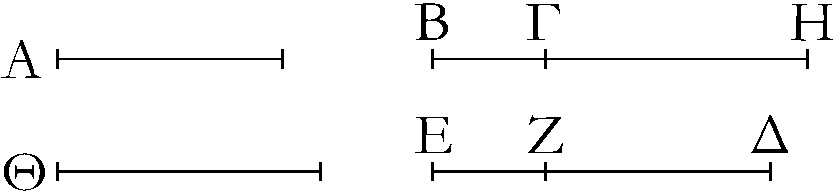
\includegraphics{Book10/fig085g.pdf}}

\gr{Ἐκκείσθω <ρητὴ ἡ Α, καὶ τῆ| Α μ\kern -.7pt  ήκει σύμμετροξ >έστω ἡ ΒΗ;
<ρητὴ >άρα ἐστὶ καὶ ἡ ΒΗ. καὶ ἐκκείσθωσαν δύο τετράγωνοι
ἀριθμοὶ οἱ ΔΕ, ΕΖ, <ῶν ἡ ὑπεροθὴ ὁ ΖΔ μ\kern -.7pt  ὴ >έστω τετράγωνοξ;
οὐδ> >άρα ὁ ΕΔ πρὸξ τὸν ΔΖ λόγον >έθει, <ὸν τετράγωνοξ
ἀριθμὸξ πρὸξ τετράγωνον ἀριθμόν. καὶ πεποιήσθω ὡξ ὁ
ΕΔ πρὸξ τὸν ΔΖ, ο<ύτωξ τὸ ἀπὸ τῆξ ΒΗ τετράγωνον πρὸξ τὸ ἀπὸ
τὴξ ΗΓ τετράγωνον; σύμμετρον >άρα ἐστὶ τὸ ἀπὸ τῆξ ΒΗ τῶ|
ἀπὸ τῆξ ΗΓ. <ρητὸν δὲ τὸ ἀπὸ τῆξ ΒΗ; <ρητὸν >άρα καὶ τὸ
ἀπὸ τῆξ ΗΓ; <ρητὴ >άρα ἐστὶ καὶ ἡ ΗΓ. καὶ ἐπεὶ ὁ ΕΔ πρὸξ 
τὸν ΔΖ λόγον οὐκ >έθει, <ὸν τετράγωνοξ ἀριθμὸξ πρὸξ τετράγωνον
ἀριθμόν, οὐδ> >άρα τὸ ἀπὸ τῆξ ΒΗ πρὸξ τὸ ἀπὸ τῆξ ΗΓ
λόγον >έθει, <ὸν τετράγωνοξ ἀριθμὸξ πρὸξ τετράγωνον
ἀριθμόν; ἀσύμμετροξ >άρα ἐστὶν ἡ ΒΗ τῆ| ΗΓ μ\kern -.5pt  ήκει.
καί εἰσιν ἀμφότεραι <ρηταί; αἱ ΒΗ, ΗΓ >άρα <ρηταί εἰσι
δυνάμει μόνον σύμμετροι; ἡ >άρα ΒΓ ἀποτομ\kern -.3pt  ή ἐστιν. λέγω
δή, <ότι καὶ πρώτη.}

\gr{<~Ωι γὰρ μεῖζόν ἐστι τὸ ἀπὸ τῆξ ΒΗ τοῦ ἀπὸ τῆξ ΗΓ, >έστω
τὸ ἀπὸ τῆξ Θ. καὶ ἐπεί ἐστιν ὡξ ὁ ΕΔ πρὸξ τὸν ΖΔ,
ο<ύτωξ τὸ ἀπὸ τῆξ ΒΗ πρὸξ τὸ ἀπὸ τῆξ ΗΓ, καὶ ἀναστρέψαντι
>άρα ἐστὶν ὡξ ὁ ΔΕ πρὸξ τὸν ΕΖ, ο<ύτωξ τὸ ἀπὸ τῆξ ΗΒ
πρὸξ τὸ ἀπὸ τῆξ Θ. ὁ δὲ ΔΕ πρὸξ τὸν ΕΖ λόγον >έθει, <ὸν
τετράγωνοξ ἀριθμὸξ πρὸξ τετράγωνον ἀριθμόν; ἑκάτεροξ
γὰρ τετράγωνόξ ἐστιν; καὶ τὸ ἀπὸ τῆξ ΗΒ >άρα πρὸξ τὸ
ἀπὸ τῆξ Θ λόγον >έθει, <ὸν τετράγωνοξ ἀριθμὸξ πρὸξ
τετράγωνον ἀριθμόν; σύμμετροξ >άρα ἐστὶν ἡ ΒΗ τῆ| Θ μ\kern -.7pt  ήκει.
καὶ δύναται ἡ ΒΗ τῆξ ΗΓ μεῖζον τῶ| ἀπὸ τῆξ Θ; ἡ ΒΗ >άρα
τῆξ ΗΓ μεῖζον δύναται τῶ| ἀπὸ συμμέτρου ἑαυτῆ| μ\kern -.7pt  ήκει.
καί ἐστιν ἡ <όλη ἡ ΒΗ σύμμετροξ τῆ| ἐκκειμένῃ <ρητῆ| μ\kern -.5pt  ήκει
τῆ| Α. ἡ ΒΓ >άρα ἀποτομ\kern -.3pt  ή ἐστι πρώτη.}

\gr{Ε<ύρηται >άρα ἡ πρώτη ἀποτομ\kern -.7pt  ὴ ἡ ΒΓ; <όπερ >έδει εὑρεῖν.}}

\ParallelRText{
\begin{center}
{\large Proposition 85}
\end{center}

To find a first apotome.

% Removed epsf size command
\centerline{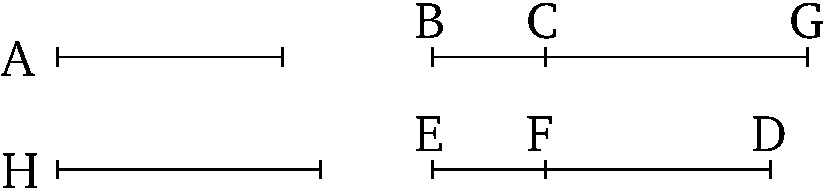
\includegraphics{Book10/fig085e.pdf}}

Let the rational (straight-line) $A$ be laid down. And let $BG$
be commensurable in length with $A$. $BG$ is thus also a rational (straight-line).
And let two square numbers
$DE$ and $EF$ be laid down, and let their difference $FD$ be  not 
square [Prop.~10.28~lem.~I]. Thus,
$ED$ does not have to $DF$ the ratio which (some) square number
(has) to (some) square number. And let it be contrived that
as $ED$ (is) to $DF$, so the square on $BG$ (is) to the square on $GC$
[Prop.~10.6.~corr.]. Thus, the (square) on $BG$
is commensurable with the (square) on $GC$ [Prop.~10.6]. And the (square) on $BG$ (is)
rational. Thus, the (square) on $GC$ (is) also rational. Thus, $GC$ is also
rational. And since $ED$ does not have to $DF$ the ratio which
(some) square number (has) to (some) square number, 
the (square) on $BG$ thus does not have to the (square) on $GC$ the ratio
which (some) square number (has) to (some) square number either. Thus,
$BG$ is incommensurable in length with $GC$ [Prop.~10.9]. And they are both
rational (straight-lines). Thus, $BG$ and $GC$ are rational (straight-lines
which are) commensurable in square only. Thus, $BC$ is an apotome
[Prop.~10.73]. So, I say that (it is)
also a first (apotome).

Let the (square) on $H$ be that (area) by which the (square) on $BG$
is greater than the (square) on $GC$ [Prop.~10.13~lem.]. And since as $ED$ is to
$FD$, so the (square) on $BG$ (is) to the (square) on $GC$, thus, via
conversion, as $DE$ is to $EF$, so the (square) on $GB$ (is) to the
(square) on $H$ [Prop.~5.19~corr.]. 
And $DE$ has to $EF$ the ratio which (some) square-number
(has) to (some) square-number. For each is a square (number). 
Thus, the (square) on $GB$ also has to the (square) on $H$ the ratio which
(some) square number (has) to (some) square number. Thus, $BG$
is commensurable in length with $H$ [Prop.~10.9].
And the square on $BG$ is greater than (the square on) $GC$ by the
(square) on $H$. Thus, the square on $BG$ is greater than (the square on) $GC$ by the
(square) on (some straight-line) commensurable in length with ($BG$).
And the whole, $BG$, is commensurable in length with the (previously)
laid down rational (straight-line) $A$. Thus, $BC$ is a first
apotome [Def.~10.11].

Thus, the first apotome $BC$ has been found. (Which is) the
very thing it was required to find.}
\end{Parallel}
{\footnotesize\noindent$^\dag$ See footnote to Prop.~10.48.}

%%%%
%10.86
%%%%
\pdfbookmark[1]{Proposition 10.86}{pdf10.86}
\begin{Parallel}{}{}
\ParallelLText{
\begin{center}
{\large \ggn{86}.}
\end{center}

\gr{Εὑρεῖν τὴν δευτέραν ἀποτομ\kern -.7pt  ήν.}

\gr{Ἐκκείσθω <ρητὴ ἡ Α καὶ τῆ| Α σύμμετροξ μ\kern -.7pt  ήκει ἡ ΗΓ. <ρητὴ
>άρα ἐστὶν ἡ ΗΓ. καὶ ἐκκείσθωσαν δύο τετράγωνοι ἀριθμοὶ
οἱ ΔΕ, ΕΖ, <ῶν ἡ ὑπεροθὴ ὁ ΔΖ μ\kern -.7pt  ὴ >έστω τετράγωνοξ. καὶ
πεποιήσθω ὡξ ὁ ΖΔ πρὸξ τὸν ΔΕ, ο<ύτωξ τὸ ἀπὸ τῆξ ΓΗ τετράγωνον
πρὸξ τὸ ἀπὸ τῆξ ΗΒ τετράγωνον. σύμμετρον >άρα ἐστὶ τὸ ἀπὸ
τῆξ ΓΗ τετράγωνον τῶ| ἀπὸ τῆξ ΗΒ τετραγώνῳ. <ρητὸν δὲ τὸ
ἀπὸ τῆξ ΓΗ. <ρητὸν >άρα [ἐστὶ] καὶ τὸ ἀπὸ τῆξ ΗΒ;
<ρητὴ >άρα ἐστὶν ἡ ΒΗ. καὶ ἐπεὶ τὸ ἀπὸ τῆξ ΗΓ τετράγωνον
πρὸξ τὸ ἀπὸ τῆξ ΗΒ λόγον οὐκ >έθει, <ὸν τετράγωνοξ ἀριθμὸξ πρὸξ
τετράγωνον ἀριθμόν, ἀσύμμετρόξ ἐστιν ἡ ΓΗ τῆ| ΗΒ
μ\kern -.5pt  ήκει. καί εἰσιν ἀμφότεραι <ρηταί; αἱ ΓΗ, ΗΒ >άρα  ρηταί εἰσι
δυνάμει μόνον σύμμετροι; ἡ ΒΓ >άρα ἀποτομ\kern -.3pt  ή ἐστιν.
λέγω δή, <ότι καὶ δευτέρα.}\\~\\~\\~\\

% Removed epsf size command
\centerline{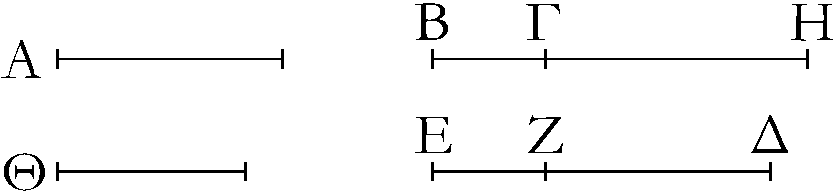
\includegraphics{Book10/fig086g.pdf}}

\gr{<~Ωι γὰρ μεῖζόν ἐστι τὸ ἀπὸ τῆξ ΒΗ τοῦ ἀπὸ τῆξ
ΗΓ, >έστω τὸ ἀπὸ τῆξ Θ. ἐπεὶ ο>ῦν ἐστιν ὡξ τὸ ἀπὸ
τῆξ ΒΗ πρὸξ τὸ ἀπὸ τῆξ ΗΓ, ο<ύτωξ ὁ ΕΔ ἀριθμὸξ
πρὸξ τὸν ΔΖ ἀριθμόν, ἀναστρέψαντι >άρα ἐστὶν ὡξ τὸ ἀπὸ
τῆξ ΒΗ πρὸξ τὸ ἀπὸ τῆξ Θ, ο<ύτωξ ὁ ΔΕ πρὸξ τὸν ΕΖ.  καί
ἐστιν ἑκάτεροξ τῶν ΔΕ, ΕΖ τετράγωνοξ; τὸ >άρα ἀπὸ τῆξ ΒΗ
πρὸξ τὸ ἀπὸ τῆξ Θ λόγον >έθει, <ὸν τετράγωνοξ ἀριθμὸξ
πρὸξ τετράγωνον ἀριθμόν; σύμμετροξ >άρα ἐστὶν ἡ ΒΗ τῆ| Θ
μ\kern -.7pt  ήκει. καὶ δύναται ἡ ΒΗ τῆξ ΗΓ μεῖζον τῶ| ἀπὸ τῆξ Θ;
ἡ ΒΗ >άρα τῆξ ΗΓ μεῖζον δύναται τῶ| ἀπὸ συμμέτρου
ἑαυτῆ| μ\kern -.7pt  ήκει. καί ἐστιν ἡ προσαρμόζουσα ἡ ΓΗ τῆ|
ἐκκειμένῃ <ρητῆ| σύμμετροξ τῆ| Α. ἡ ΒΓ >άρα ἀποτομ\kern -.5pt  ή
ἐστι δευτέτα.}

\gr{Ε<ύρηται >άρα δευτέρα ἀποτομ\kern -.7pt  ὴ ἡ ΒΓ;
<όπερ >έδει δεῖχαι.}}

\ParallelRText{
\begin{center}
{\large Proposition 86}
\end{center}\vspace*{-7pt}

To find a second apotome.

Let the rational (straight-line) $A$, and $GC$ (which is)
commensurable in length with $A$, be laid down. Thus, $GC$ is a rational (straight-line).
And let the two square numbers $DE$ and $EF$ be laid down, and let
their
difference $DF$ be not square [Prop.~10.28~lem.~I]. 
And let it be contrived that as $FD$ (is) to $DE$, so the square on $CG$ (is) to the square on $GB$ [Prop.~10.6~corr.].
Thus, the square on $CG$ is commensurable with the square on $GB$ [Prop.~10.6]. And the (square) on $CG$ (is) rational.
Thus, the (square) on $GB$ [is] also rational. Thus, $BG$ is a rational
(straight-line).  And since the square on $GC$ does not have to the
(square) on $GB$ the ratio which (some) square number (has) to
(some) square number, $CG$ is incommensurable in length with $GB$
[Prop.~10.9]. And they are both rational (straight-lines). Thus, $CG$ and $GB$ are rational (straight-lines which are)
commensurable in square only. Thus, $BC$ is an apotome [Prop.~10.73]. So, I say that it is also a second
(apotome).

% Removed epsf size command
\centerline{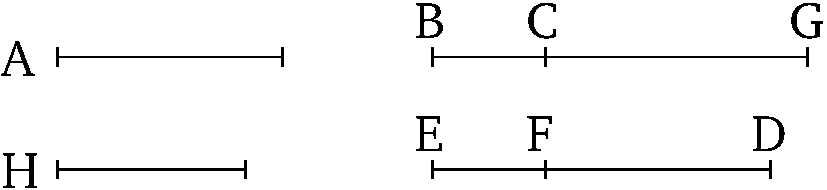
\includegraphics{Book10/fig086e.pdf}}

For let the (square) on $H$ be that (area) by which the (square) on $BG$
is greater than the (square) on $GC$ [Prop.~10.1 lem.]. Therefore, since
as the (square) on $BG$ is to the (square) on $GC$, so the number $ED$
(is) to the number $DF$, thus, also, via conversion, as the (square) on $BG$
is to the (square) on $H$, so $DE$ (is) to $EF$ [Prop.~5.19~corr.]. And $DE$ and $EF$ are each
square (numbers). Thus, the (square) on $BG$ has to the (square)
on $H$ the ratio which (some) square number (has) to (some) square number.
Thus, $BG$ is commensurable in length with $H$ [Prop.~10.9]. 
And the square on $BG$ is greater than (the square on) $GC$ by the (square)
on $H$.
Thus, the square on $BG$ is greater
than (the square on) $GC$ by the (square) on (some straight-line)
commensurable in length with ($BG$). And the attachment $CG$
is commensurable (in length) with the (prevously) laid down rational (straight-line) $A$.
Thus, $BC$ is a second apotome [Def.~10.12].$^\dag$

Thus, the second apotome $BC$ has been found. (Which is) the very thing
it was required to show.}
\end{Parallel}
{\footnotesize\noindent$^\dag$ See footnote to Prop.~10.49.}

%%%%
%10.87
%%%%
\pdfbookmark[1]{Proposition 10.87}{pdf10.87}
\begin{Parallel}{}{}
\ParallelLText{
\begin{center}
{\large \ggn{87}.}
\end{center}\vspace*{-7pt}

\gr{Εὑρεῖν τὴν τρίτην ἀποτομ\kern -.7pt  ήν.}

% Removed epsf size command
\centerline{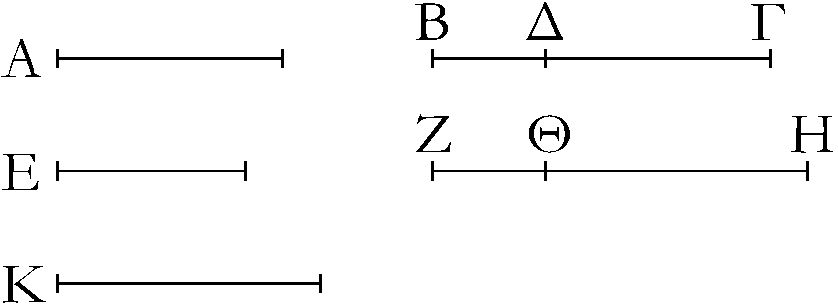
\includegraphics{Book10/fig087g.pdf}}

\gr{Ἐκκείσθω <ρητὴ ἡ Α, καὶ ἐκκείσθωσαν τρεῖξ ἀριθμοὶ
οἱ Ε, ΒΓ, ΓΔ λόγον μ\kern -.7pt  ὴ >έθοντεξ πρὸξ ἀλλήλουξ, <ὸν
τετράγωνοξ ἀριθμὸξ πρὸξ τετράγωνον ἀριθμόν, ὁ δὲ
ΓΒ πρὸξ τὸν ΒΔ λόγον ἐθέτω, <ὸν τετράγωνοξ ἀριθμὸξ πρὸξ
τετράγωνον ἀριθμόν, καὶ πεποιήσθω ὡξ μὲν ὁ Ε πρὸξ τὸν
ΒΓ, ο<ύτωξ τὸ ἀπὸ τῆξ Α τετράγωνον πρὸξ τὸ ἀπὸ τῆξ
ΖΗ τετράγωνον, ὡξ δὲ ὁ ΒΓ πρὸξ τὸν ΓΔ, ο<ύτωξ τὸ ἀπὸ
τῆξ ΖΗ τετράγωνον πρὸξ τὸ ἀπὸ τὴξ ΗΘ. ἐπεὶ ο>ῦν ἐστιν
ὡξ ὁ Ε πρὸξ τὸν ΒΓ, ο<ύτωξ τὸ ἀπὸ τῆξ Α τετράγωνον πρὸξ
τὸ ἀπὸ τῆξ ΖΗ τετράγωνον, σύμμετρον >άρα ἐστὶ τὸ ἀπὸ
τῆξ Α τετράγωνον τῶ| ἀπὸ τῆξ ΖΗ τετραγώνῳ. <ρητὸν δὲ
τὸ ἀπὸ τῆξ Α τετράγωνον. <ρητὸν >άρα καὶ τὸ ἀπὸ τῆξ ΖΗ;
<ρητὴ >άρα ἐστὶν ἡ ΖΗ. καὶ ἐπεὶ ὁ Ε πρὸξ τὸν ΒΓ
λόγον οὐκ >έθει, <ὸν τετράγωνοξ ἀριθμὸξ πρὸξ τετράγωνον
ἀριθμόν, οὐδ> >άρα τὸ ἀπὸ τῆξ Α
τετράγωνον πρὸξ τὸ ἀπὸ τῆξ ΖΗ [τετράγωνον] λόγον >έθει,
<όν τετράγωνοξ ἀριθμὸξ πρὸξ τετράγωνον ἀριθμόν; ἀσύμμετροξ
>άρα ἐστὶν ἡ Α τῆ| ΖΗ μ\kern -.7pt  ήκει. πάλιν, ἐπεί ἐστιν ὡξ ὁ ΒΓ
πρὸξ τὸν ΓΔ, ο<ύτωξ τὸ ἀπὸ τῆξ ΖΗ τετράγωνον πρὸξ τὸ ἀπὸ
τῆξ ΗΘ, σύμμετρον >άρα ἐστὶ τὸ ἀπὸ τῆξ ΖΗ τῶ| ἀπὸ τῆξ ΗΘ.
<ρητὸν δὲ τὸ ἀπὸ τῆξ ΖΗ; <ρητὸν >άρα καὶ τὸ ἀπὸ τῆξ ΗΘ; <ρητὴ
>άρα ἐστὶν ἡ ΗΘ. καὶ ἐπεὶ ὁ ΒΓ πρὸξ τὸν ΓΔ λόγον οὐκ
>έθει, <ὸν τετράγωνοξ ἀριθμὸξ πρὸξ τετράγωνον ἀριθμόν, οὐδ>
>άρα τὸ ἀπὸ τῆξ ΖΗ πρὸξ τὸ ἀπὸ τῆξ ΗΘ λόγον >έθει, <ὸν
τετράγωνοξ ἀριθμὸξ πρὸξ τετράγωνον ἀριθμόν;
ἀσύμμετροξ >άρα ἐστὶν ἡ ΖΗ τῆ| ΗΘ μ\kern -.5pt  ήκει. καί εἰσιν ἀμφότεραι
<ρηταί; αἱ ΖΗ, ΗΘ >άρα <ρηταί εἰσι δυνάμει μόνον σύμμετροι;
ἀποτομ\kern -.3pt  ὴ >άρα ἐστὶν ἡ ΖΘ. λέγω δή, <ότι καὶ τρίτη.}

\gr{Ἐπεὶ γάρ ἐστιν ὡξ μὲν ὁ Ε πρὸξ τὸν ΒΓ, ο<ύτωξ τὸ ἀπὸ τῆξ
Α τετράγωνον πρὸξ τὸ ἀπὸ τῆξ ΖΗ, ὡξ δὲ ὁ ΒΓ πρὸξ τὸν ΓΔ,
ο<ύτωξ τὸ ἀπὸ τῆξ ΖΗ πρὸξ  τὸ ἀπὸ τῆξ ΘΗ, δι> >ίσου >άρα
ἐστὶν ὡξ ὁ Ε πρὸξ τὸν ΓΔ, ο<ύτωξ τὸ ἀπὸ τῆξ Α πρὸξ τὸ
ἀπὸ τῆξ ΘΗ. ὁ δὲ Ε πρὸξ τὸν ΓΔ λόγον οὐκ >έθει, <ὸν
τετράγωνοξ ἀριθμὸξ πρὸξ τετράγωνον ἀριθμόν; οὐδ> >άρα τὸ
ἀπὸ τῆξ Α πρὸξ τὸ ἀπὸ τῆξ ΗΘ λόγον >έθει, <ὸν τετράγωνοξ
ἀριθμὸξ
πρὸξ τετράγωνον ἀριθμόν; ἀσύμμετροξ >άρα ἡ Α τῆ| ΗΘ
μ\kern -.7pt  ήκει. οὐδετέρα >άρα τῶν ΖΗ, ΗΘ σύμμετρόξ ἐστι τῆ| ἐκκειμένῃ
<ρητῆ| τῆ| Α μ\kern -.7pt  ήκει. <ῶ| ο>ῦν μεῖζόν ἐστι τὸ ἀπὸ τῆξ ΖΗ
τοῦ ἀπὸ τῆξ ΗΘ, >έστω τὸ ἀπὸ τῆξ Κ. ἐπεὶ ο>ῦν ἐστιν ὡξ
ὁ ΒΓ πρὸξ τὸν ΓΔ, ο<ύτωξ τὸ ἀπὸ τῆξ ΖΗ πρὸξ τὸ ἀπὸ τῆξ
ΗΘ, ἀναστρέψαντι >άρα ἐστὶν ὡξ ὁ ΒΓ πρὸξ τὸν ΒΔ, ο<ύτωξ
τὸ ἀπὸ τῆξ ΖΗ τετράγωνον πρὸξ τὸ ἀπὸ τῆξ Κ. ὁ δὲ
ΒΓ πρὸξ τὸν ΒΔ λόγον >έθει, <ὸν τετράγωνοξ ἀριθμὸξ πρὸξ
τετράγωνον ἀριθμόν. καὶ τὸ ἁπὸ τῆξ ΖΗ >άρα πρὸξ τὸ ἀπὸ
τῆξ Κ λόγον >έθει, <ὸν τετράγωνοξ ἀριθμὸξ πρὸξ τετράγωνον ἀριθμόν.
σύμμετρόξ >άρα ἐστὶν ἡ ΖΗ τῆ| Κ μ\kern -.5pt  ήκει,
καὶ δύναται ἡ ΖΗ τῆξ ΗΘ μεῖζον τῶ| ἀπὸ συμμέτρου ἑαυτῆ|.
καὶ οὐδετέρα τῶν ΖΗ, ΗΘ σύμμετρόξ ἐστι τῆ| ἐκκειμένῃ <ρητῆ|
τῆ| Α μ\kern -.3pt  ήκει; ἡ ΖΘ >άρα ἀποτομ\kern -.7pt  ή ἐστι τρίτη.}

\gr{Ε<ύρηται >άρα ἡ τρίτη ἀποτομ\kern -.7pt  ὴ ἡ ΖΘ; <όπερ
>έδει δεῖχαι.}}

\ParallelRText{
\begin{center}
{\large Proposition 87}
\end{center}

To find a third apotome.

% Removed epsf size command
\centerline{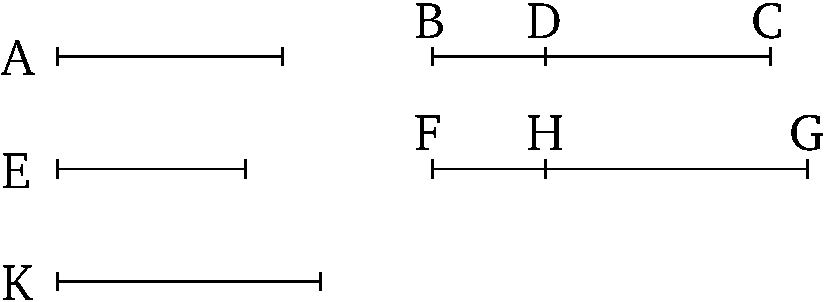
\includegraphics{Book10/fig087e.pdf}}

Let the rational (straight-line) $A$ be laid down. And let the
three numbers, $E$, $BC$, and $CD$, not having to one another
the ratio which (some) square number (has) to (some) square number,
be laid down. And let $CB$ have to $BD$ the ratio which (some)
square number (has) to (some) square number. And let it be
contrived that as $E$ (is) to $BC$, so the square on $A$ (is) to the square
on $FG$, and as $BC$ (is) to $CD$, so the square on $FG$ (is) to the (square)
on $GH$ [Prop.~10.6~corr.]. Therefore,
since  as $E$ is to $BC$, so the square on $A$ (is) to the square on
$FG$, the square on $A$ is thus commensurable with the square on
$FG$ [Prop.~10.6]. And the square on $A$
(is) rational. Thus, the (square) on $FG$ (is) also rational. Thus,
$FG$ is a rational (straight-line). And since  $E$ does not have to $BC$
the ratio which (some) square number (has) to (some) square number,
the square on $A$ thus does not have to the [square] on $FG$ the ratio
which (some) square number (has) to (some) square number either. Thus,
$A$ is incommensurable in length with $FG$ [Prop.~10.9]. Again, since as $BC$ is to $CD$, so
the square on $FG$ is to the (square) on $GH$, the square on $FG$
is thus commensurable with the (square) on $GH$ [Prop.~10.6]. And the (square) on $FG$ (is)
rational. Thus, the (square) on $GH$ (is) also rational. Thus, $GH$ is
a rational (straight-line). And since $BC$ does not have to $CD$ the
ratio which (some) square number (has) to (some) square number, the
(square) on $FG$ thus does not have to the (square) on $GH$ the
ratio which (some) square number (has) to (some) square number either.
Thus, $FG$ is incommensurable in length with $GH$ [Prop.~10.9]. And both are rational (straight-lines).
$FG$ and $GH$ are thus rational (straight-lines which are) commensurable
in square only. Thus, $FH$ is an apotome [Prop.~10.73]. So, I say that (it is) also a third
(apotome).

For since as $E$ is to $BC$, so the square on $A$ (is) to the (square)
on $FG$, and as $BC$ (is) to $CD$, so the (square) on $FG$
(is) to the (square) on $HG$, thus, via equality, as $E$ is to
$CD$, so the (square) on $A$ (is) to the (square) on $HG$ [Prop.~5.22]. And $E$ does not have to $CD$
the ratio which (some) square number (has) to (some) square number. Thus,
the (square) on $A$ does not have to the (square) on $GH$ the ratio
which (some) square number (has) to (some) square number either. 
$A$ (is) thus incommensurable in length with $GH$ [Prop.~10.9]. Thus, neither of $FG$ and $GH$
is commensurable in length with the (previously) laid down rational
(straight-line) $A$. Therefore, let the (square) on $K$ be that (area) by which the (square) on
$FG$ is greater than the (square) on $GH$ [Prop.~10.13~lem.]. Therefore, since as $BC$ is to
$CD$, so the (square) on $FG$ (is) to the (square) on $GH$, thus,
via conversion, as $BC$ is to $BD$, so the square on $FG$ (is) to the square on
$K$ [Prop.~5.19~corr.]. And $BC$ has to $BD$ the ratio which
(some) square number (has) to (some) square number. Thus, the (square)
on $FG$ also has to the (square) on $K$ the ratio which (some)
square number (has) to (some) square number.
$FG$ is thus commensurable in length with $K$ [Prop.~10.9]. And the square on $FG$ is (thus) greater
than (the square on) $GH$ by the (square) on (some straight-line)
commensurable (in length) with ($FG$). And neither of $FG$ and
$GH$ is commensurable in length with the (previously) laid down
rational (straight-line) $A$. Thus, $FH$ is a third
apotome [Def.~10.13].

Thus, the third apotome $FH$ has been found. (Which is) very thing
it was required to show.}
\end{Parallel}
{\footnotesize\noindent$^\dag$ See footnote
to Prop.~10.50.}

%%%%
%10.88
%%%%
\pdfbookmark[1]{Proposition 10.88}{pdf10.88}
\begin{Parallel}{}{}
\ParallelLText{
\begin{center}
{\large\ggn{88}.}
\end{center}\vspace*{-7pt}

\gr{Εὑρεῖν τὴν τετάρτην ἀποτομ\kern -.7pt  ήν.}

% Removed epsf size command
\centerline{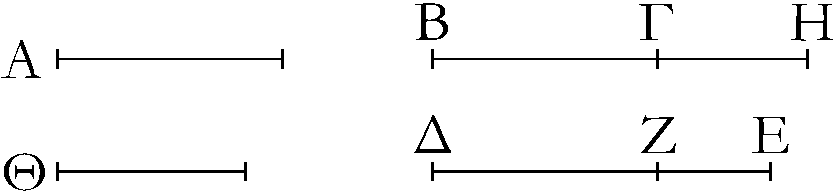
\includegraphics{Book10/fig088g.pdf}}

\gr{Ἐκκείσθω <ρητὴ ἡ Α καὶ τῆ| Α μ\kern -.7pt  ήκει σύμμετροξ ἡ ΒΗ;
<ρητὴ >άρα ἐστὶ καὶ ἡ ΒΗ. καὶ ἐκκείσθωσαν δύο ἀριθμοὶ οἱ ΔΖ, ΖΕ,
<ώστε τὸν ΔΕ <όλον πρὸξ ἑκάτερον τῶν ΔΖ, ΕΖ λόγον μ\kern -.7pt  ὴ
>έθειν, <ὸν τετράγωνοξ ἀριθμὸξ πρὸξ τετράγωνον ἀριθμόν. καὶ
πεποιήσθω ὡξ ὁ ΔΕ πρὸξ τὸν ΕΖ, ο<ύτωξ τὸ ἀπὸ τῆξ ΒΗ
τετράγωνον πρὸξ τὸ ἀπὸ τῆξ ΗΓ; σύμμετρον >άρα ἐστὶ τὸ
ἀπὸ τῆξ ΒΗ τῶ| ἀπὸ τῆξ ΗΓ.
 <ρητὸν δὲ τὸ ἀπὸ τῆξ ΒΗ; 
 <ρητὸν >άρα καὶ τὸ ἀπὸ τῆξ ΗΓ; 
 <ρητὴ >άρα ἐστὶν ἡ ΗΓ.
καὶ ἐπεὶ ὁ ΔΕ πρὸξ τὸν ΕΖ λόγον οὐκ >έθει, <ὸν τετράγωνοξ ἀριθμὸξ πρὸξ τετράγωνον ἀριθμόν, οὐδ> >άρα τὸ ἀπὸ τῆξ
ΒΗ πρὸξ τὸ ἀπὸ τῆξ ΗΓ λόγον >έθει, <ὸν τετράγωνοξ ἀριθμὸξ
πρὸξ τετράγωνον ἀριθμόν;
ἀσύμμετροξ >άρα ἐστὶν ἡ ΒΗ τῆ| ΗΓ μ\kern -.5pt  ήκει. καί εἰσιν ἀμφότεραι
<ρηταί; αἱ ΒΗ, ΗΓ >άρα <ρηταί εἰσι δυνάμει μόνον σύμμετροι;
ἀποτομ\kern -.3pt  ὴ >άρα ἐστὶν ἡ ΒΓ.  [λέγω δή, <ότι καὶ τετάρτη.]}

\gr{<~Ωι ο>ῦν μεῖζόν ἐστι τὸ ἀπὸ τῆξ ΒΗ τοῦ ἀπὸ τῆξ
ΗΓ, >έστω τὸ ἀπὸ τῆξ Θ. ἐπεὶ ο>ῦν ἐστιν ὡξ ὁ ΔΕ πρὸξ
τὸν ΕΖ, ο<ύτωξ τὸ ἀπὸ τῆξ ΒΗ πρὸξ τὸ ἀπὸ τῆξ
ΗΓ, καὶ ἀναστρέψαντι >άρα ἐστὶν ὡξ ὁ ΕΔ πρὸξ τὸν ΔΖ,
ο<ύτωξ τὸ ἀπὸ τῆξ ΗΒ πρὸξ τὸ  ἀπὸ τῆξ Θ.
ὁ δὲ ΕΔ πρὸξ τὸν ΔΖ λόγον οὐκ >έθει, <ὸν τετράγωνοξ
ἀριθμὸξ πρὸξ τετράγωνον ἀριθμόν; οὐδ> >άρα τὸ ἀπὸ τῆξ ΗΒ
πρὸξ τὸ ἀπὸ τῆξ Θ λόγον >έθει, <ὸν τετράγωνοξ ἀριθμὸξ
πρὸξ τετράγωνον ἀριθμόν;
 ἀσύμμετροξ >άρα ἐστὶν
ἡ ΒΗ τῆ| Θ μ\kern -.7pt  ήκει. καὶ δύναται ἡ ΒΗ τῆξ ΗΓ μεῖζον τῶ|
ἀπὸ τῆξ Θ; ἡ >άρα ΒΗ τῆξ ΗΓ μεῖζον δύναται
τῶ| ἀπὸ ἀσυμμέτρου ἑαυτῆ|.
καὶ ἐστιν <όλη ἡ ΒΗ
 σύμμετροξ τῆ| ἐκκειμένῃ <ρητῆ| μ\kern -.7pt  ήκει τῆ| Α.
ἡ >άρα ΒΓ ἀποτομ\kern -.5pt  ή ἐστι τετάρτη.}

\gr{Ε<ύρηται >άρα ἡ τετάρτη ἀποτομ\kern -.7pt  ή; <όπερ >έδει δεῖχαι.}}

\ParallelRText{
\begin{center}
{\large Proposition 88}
\end{center}

To find a fourth apotome.

% Removed epsf size command
\centerline{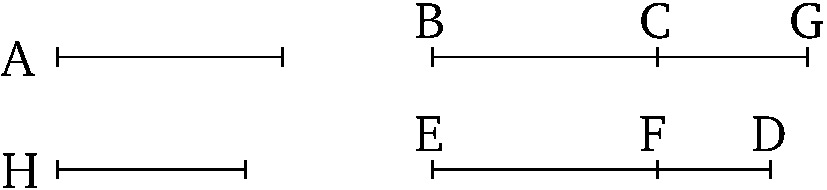
\includegraphics{Book10/fig088e.pdf}}

Let the rational (straight-line) $A$, and $BG$ (which is)
commensurable in length with $A$, be laid down.
Thus, $BG$ is also a rational (straight-line). And let the two numbers $DF$
and $FE$ be laid down such that the whole, $DE$, does not have to
each of $DF$ and $EF$ the ratio which (some) square number (has)
to (some) square number. And let it be contrived that as $DE$
(is) to $EF$, so the square on $BG$ (is) to the (square) on $GC$
[Prop.~10.6~corr.]. The (square) on $BG$ is
thus commensurable with the (square) on $GC$ [Prop.~10.6]. And the (square) on $BG$ (is)
rational. Thus, the (square) on $GC$ (is) also rational. Thus, $GC$
(is) a rational (straight-line). And since $DE$ does not have to $EF$
the ratio which (some) square number (has) to (some) square number,
the (square) on $BG$ thus does not have to the (square) on $GC$ the
ratio which (some) square number (has) to (some) square number either.
Thus, $BG$ is incommensurable in length with $GC$ [Prop.~10.9]. And they are both rational (straight-lines). Thus, $BG$ and $GC$ are rational (straight-lines which are)
commensurable in square only. Thus, $BC$ is an apotome [Prop.~10.73]. [So, I say that
(it is) also a fourth (apotome).]

Now, let the (square) on $H$ be that (area) by which the (square)
on $BG$ is greater than the (square) on $GC$ [Prop.~10.13~lem.]. Therefore, since as
$DE$ is to $EF$, so the (square) on $BG$ (is) to the (square)
on $GC$, thus, also, via conversion, as $ED$ is to $DF$, so the
(square) on $GB$ (is) to the (square) on $H$ [Prop.~5.19~corr.]. And $ED$ does not have to
$DF$ the ratio which (some) square number (has) to (some) square number.
Thus, the (square) on $GB$ does not have to the (square) on $H$
the ratio which (some) square number (has) to (some) square number either.
Thus, $BG$ is incommensurable in length with $H$ [Prop.~10.9]. And the square on $BG$ is greater
than (the square on) $GC$ by the (square) on $H$. Thus, the
square on $BG$ is greater than (the square) on $GC$ by the (square)
on (some straight-line) incommensurable (in length) with ($BG$). And the whole,
$BG$, is commensurable in length with the the (previously) laid
down rational (straight-line) $A$. Thus, $BC$ is a fourth apotome
[Def.~10.14].$^\dag$

Thus, a fourth apotome has been found. (Which is) the very thing it was required to show.}
\end{Parallel}
{\footnotesize\noindent$^\dag$ See footnote to Prop.~10.51.}

%%%%
%10.89
%%%%
\pdfbookmark[1]{Proposition 10.89}{pdf10.89}
\begin{Parallel}{}{}
\ParallelLText{
\begin{center}
{\large \ggn{89}.}
\end{center}\vspace*{-7pt}

\gr{Εὐρεῖν τὴν πέμπτην ἀποτομ\kern -.7pt  ήν.}

% Removed epsf size command
\centerline{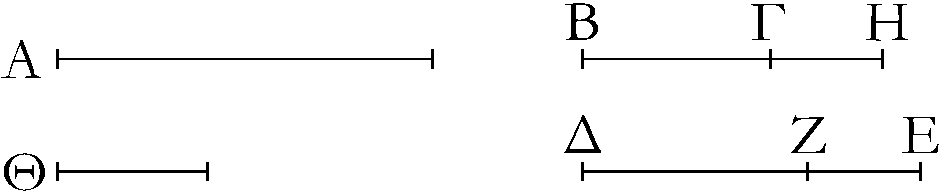
\includegraphics{Book10/fig089g.pdf}}

\gr{Ἐκκείσθω <ρητὴ ἡ Α, καὶ τῆ| Α μ\kern -.7pt  ήκει σύμμετροξ >έστω ἡ ΓΗ;
<ρητὴ >άρα [ἐστὶν] ἡ ΓΗ. καὶ ἐκκείσθωσαν δύο ἀριθμοὶ
οἱ ΔΖ, ΖΕ, <ώστε τὸν ΔΕ πρὸξ ἑκάτερον τῶν ΔΖ, ΖΕ λόγον
πάλιν μ\kern -.7pt  ὴ >έθειν, <ὸν τετράγωνοξ ἀριθμὸξ πρὸξ τετράγωνον
ἀριθμόν; 
καὶ πεποιήσθω ὡξ ὁ ΖΕ πρὸξ τὸν ΕΔ, ο<ύτωξ τὸ ἀπὸ τῆξ
ΓΗ πρὸξ τὸ ἀπὸ τῆξ ΗΒ. 
<ρητὸν >άρα καὶ τὸ ἀπὸ τῆξ ΗΒ; 
<ρητὴ >άρα ἐστὶ καὶ ἡ ΒΗ. 
καὶ
ἐπεί ἐστιν ὡξ ὁ ΔΕ πρὸξ τὸν ΕΖ, ο<ύτωξ τὸ ἀπὸ τῆξ ΒΗ
πρὸξ τὸ ἀπὸ τῆξ ΗΓ, ὁ δὲ ΔΕ πρὸξ τὸν ΕΖ λόγον οὐκ
>έθει, <ὸν τετράγωνοξ ἀριθμὸξ πρὸξ τετράγωνον ἀριθμόν,
οὐδ> >άρα τὸ ἀπὸ τῆξ ΒΗ πρὸξ τὸ ἀπὸ τῆξ ΗΓ λόγον
>έθει, <ὸν τετράγωνοξ ἀριθμὸξ πρὸξ τετράγωνον ἀριθμόν;
ἀσύμμετροξ >άρα ἐστὶν ἡ ΒΗ τῆ| ΗΓ μ\kern -.5pt  ήκει. καί εἰσιν
ἀμφότεραι <ρηταί; αἱ ΒΗ, ΗΓ >άρα <ρηταί εἰσι δυνάμει
μόνον σύμμετροι; ἡ ΒΓ >άρα ἀποτομ\kern -.3pt  ή ἐστιν. λέγω δή,
<ότι καὶ πέμπτη.}

\gr{<~Ωι γὰρ μεῖζόν ἐστι τὸ ἀπὸ τῆξ ΒΗ τοῦ ἀπὸ τῆξ
ΗΓ, >έστω τὸ ἀπὸ τῆξ Θ. ἐπεὶ ο>ῦν ἐστιν ὡξ τὸ ἀπὸ
τὴξ ΒΗ πρὸξ τὸ ἀπὸ τῆξ ΗΓ, ο<ύτωξ ὁ ΔΕ πρὸξ τὸν ΕΖ,
ἀναστρέψαντι >άρα ἐστὶν  ὡξ ὁ ΕΔ πρὸξ τὸν ΔΖ, ο<ύτωξ
τὸ ἀπὸ τῆξ ΒΗ πρὸξ τὸ ἀπὸ τῆξ Θ, ὁ δὲ ΕΔ πρὸξ τὸν ΔΖ
λόγον οὐκ >έθει, <ὸν τετράγωνοξ ἀριθμὸξ πρὸξ τετράγωνον
ἀριθμόν; οὐδ> >άρα τὸ ἀπὸ τῆξ ΒΗ πρὸξ τὸ ἀπὸ τῆξ Θ
λόγον >έθει, <ὸν τετράγωνοξ ἀριθμὸξ πρὸξ τετράγωνον ἀριθμόν;
ἀσύμμετροξ >άρα ἐστὶν ἡ ΒΗ τῆ| Θ μ\kern -.7pt  ήκει. καὶ δύναται
ἡ ΒΗ τῆξ ΗΓ μεῖζον τῶ| ἀπὸ τῆξ Θ; ἡ ΗΒ >άρα τῆξ ΗΓ
μεῖζον δύναται τῶ| ἀπὸ ἀσυμμέτρου ἑαυτῆ| μ\kern -.7pt  ήκει. καί
ἐστιν ἡ προσαρμόζουσα ἡ ΓΗ σύμμετροξ τῆ| ἐκκειμένῃ <ρητῆ|
τῆ| Α μ\kern -.5pt  ήκει; ἡ >άρα ΒΓ ἀποτομ\kern -.3pt  ή ἐστι πέμπτη.}

\gr{Ε<ύρηται >άρα ἡ πέμπτη ἀποτομ\kern -.7pt  ὴ ἡ ΒΓ;
<όπερ >έδει δεῖχαι.}}

\ParallelRText{
\begin{center}
{\large Proposition 89}
\end{center}

To find a fifth apotome.

% Removed epsf size command
\centerline{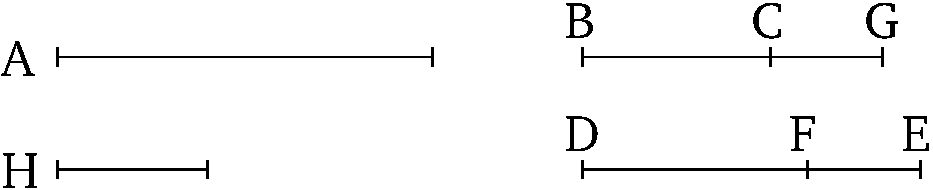
\includegraphics{Book10/fig089e.pdf}}

Let the rational (straight-line) $A$ be laid down, and let
$CG$ be commensurable in length with $A$. Thus, $CG$ [is] a rational
(straight-line). And let the two numbers $DF$ and $FE$ be laid
down such that $DE$ again does not have to each of $DF$ and $FE$
the ratio which (some) square number (has) to (some) square number. 
And let it be contrived that as $FE$ (is) to $ED$, so the
(square) on $CG$ (is) to the (square) on $GB$. Thus, the (square) on
$GB$ (is) also rational [Prop.~10.6]. 
Thus, $BG$ is also rational.
And since as $DE$ is to $EF$, so the (square) on $BG$ (is) to
the (square) on $GC$. And $DE$ does not have to $EF$ the
ratio which (some) square number (has) to (some) square number.
The (square) on $BG$ thus does not have to the (square) on $GC$
the ratio which (some) square number (has) to (some) square number either.
Thus, $BG$ is incommensurable in length with $GC$ [Prop.~10.9]. And they are both rational (straight-lines). $BG$ and $GC$ are thus rational (straight-lines which are)
commensurable in square only. Thus, $BC$ is an apotome [Prop.~10.73]. So, I say that (it is) also a fifth
(apotome).

For, let the (square) on $H$ be that (area) by which the (square) on $BG$
is greater than the (square) on $GC$ [Prop.~10.13~lem.]. Therefore, since
as the (square) on $BG$ (is) to the (square) on $GC$, so $DE$  (is) to
$EF$, thus, via conversion, as $ED$ is to $DF$, so the (square)
on $BG$ (is) to the (square) on $H$ [Prop.~5.19~corr.]. And $ED$ does not have to
$DF$ the ratio which (some) square number (has) to (some) square number.
Thus, the (square) on $BG$ does not have to the (square) on $H$
the ratio which (some) square number (has) to (some) square number
either. Thus, $BG$ is incommensurable in length with $H$ [Prop.~10.9]. And the square on $BG$ is greater
than (the square on) $GC$ by the (square) on $H$.
Thus, the square on $GB$ is greater
than (the square on) $GC$ by the (square) on (some straight-line)
incommensurable in length with ($GB$). And the attachment $CG$ is
commensurable in length with the (previously) laid down rational (straight-line) $A$. Thus, $BC$ is a fifth apotome [Def.~10.15].$^\dag$

Thus, the fifth apotome $BC$ has been found. (Which is) the very thing it
was required to show.}
\end{Parallel}
{\footnotesize\noindent$^\dag$ See footnote to Prop.~10.52.}

%%%%
%10.90
%%%%
\pdfbookmark[1]{Proposition 10.90}{pdf10.90}
\begin{Parallel}{}{}
\ParallelLText{
\begin{center}
{\large \ggn{90}.}
\end{center}

\gr{Εὑρεῖν τὴν <έκτην ἀποτομ\kern -.7pt  ήν.}

\gr{Ἐκκείσθω <ρητὴ ἡ Α καὶ τρεῖξ ἀριθμοὶ οἱ Ε, ΒΓ, ΓΔ
λόγον μ\kern -.7pt  ὴ >έθοντεξ πρὸξ ἀλλήλουξ, <ὸν τετράγωνοξ ἀριθμὸξ
πρὸξ τετράγωνον ἀριθμόν; >έτι δὲ καὶ ὁ ΓΒ πρὸξ τὸν ΒΔ λόγον
μ\kern -.7pt  ὴ ἐθετώ, <ὸν τετράγωνοξ ἀριθμὸξ πρὸξ τετράγωνον ἀριθμόν;
καὶ πεποιήσθω ὡξ μὲν ὁ Ε πρὸξ τὸν ΒΓ, ο<ύτωξ τὸ ἀπὸ τῆξ
Α πρὸξ τὸ ἀπὸ τῆξ ΖΗ, ὡξ δὲ ὁ ΒΓ πρὸξ τὸν ΓΔ, ο<ύτωξ τὸ ἀπὸ
τῆξ ΖΗ πρὸξ τὸ ἀπὸ τῆξ ΗΘ.}\\

% Removed epsf size command
\centerline{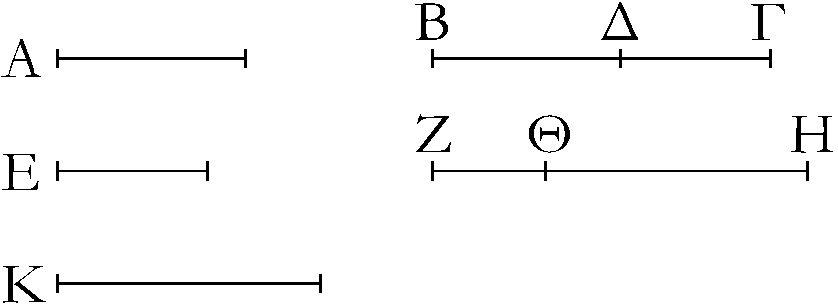
\includegraphics{Book10/fig090g.pdf}}

\gr{Ἐπεὶ ο>ῦν ἐστιν ὡξ ὁ Ε πρὸξ τὸν ΒΓ, ο<ύτωξ τὸ ἀπὸ τῆξ
Α πρὸξ τὸ ἀπὸ τῆξ ΖΗ, σύμμετρον >άρα τὸ ἀπὸ τῆξ Α τῶ|
ἀπὸ τῆξ ΖΗ. <ρητὸν δὲ τὸ ἀπὸ τῆξ Α; <ρητὸν >άρα καὶ
τὸ ἀπὸ τῆξ ΖΗ; <ρητὴ >άρα ἐστὶ καὶ ἡ ΖΗ. καὶ ἐπεὶ ὁ Ε
πρὸξ τὸν ΒΓ λόγον οὐκ >έθει, <ὸν τετράγωνοξ ἀριθμὸξ
πρὸξ τετράγωνον ἀριθμόν, οὐδ> >άρα τὸ ἀπὸ τῆξ Α πρὸξ τὸ
ἀπὸ τῆξ ΖΗ λόγον >έθει, <ὸν τετράγωνοξ ἀριθμὸξ πρὸξ τετράγωνον
ἀριθμόν; ἀσύμμετροξ >άρα ἐστὶν ἡ Α τῆ ΖΗ μ\kern -.7pt  ήκει. πάλιν,
ἐπεί ἐστιν ὡξ ὁ ΒΓ πρὸξ τὸν ΓΔ, ο<ύτωξ τὸ ἀπὸ τῆξ ΖΗ
πρὸξ τὸ ἀπὸ τῆξ ΗΘ, σύμμετρον >άρα τὸ ἀπὸ τῆξ ΖΗ τῶ|
ἀπὸ τῆξ ΗΘ. <ρητὸν δὲ τὸ ἀπὸ τῆξ ΖΗ; <ρητὸν >άρα καὶ τὸ
ἀπὸ τῆξ ΗΘ; <ρητὴ >άρα καὶ ἡ ΗΘ. καὶ ἐπεὶ ὁ ΒΓ πρὸξ
τὸν ΓΔ λόγον οὐκ >έθει, <ὸν τετράγωνοξ ἀριθμὸξ πρὸξ τετράγωνον
ἀριθμόν, οὐδ> >άρα τὸ ἀπὸ τῆξ ΖΗ πρὸξ τὸ ἀπὸ τῆξ ΗΘ
λόγον >έθει, <ὸν τετράγωνοξ ἀριθμὸξ πρὸξ τετράγωνον ἀριθμόν;
ἀσύμμετροξ >άρα ἐστὶν ἡ ΖΗ τῆ| ΗΘ μ\kern -.7pt  ήκει. καί εἰσιν
ἀμφότεραι <ρηταί; αἱ ΖΗ, ΗΘ >άρα <ρηταί εἰσι δυνάμει μόνον
σύμμετροι; ἡ >άρα ΖΘ ἀποτομ\kern -.5pt  ή ἐστιν. λέγω δή, <ότι καὶ
<έκτη.}

\gr{Ἐπεὶ γάρ ἐστιν ὡξ μὲν ὁ Ε πρὸξ τὸν ΒΓ, ο<ύτωξ τὸ ἀπὸ τῆξ
Α πρὸξ τὸ ἀπὸ τῆξ ΖΗ, ὡξ δὲ ὁ ΒΓ πρὸξ τὸν ΓΔ, ο<ύτωξ
τὸ ἀπὸ τῆξ ΖΗ πρὸξ τὸ ἀπὸ τῆξ ΗΘ, δι> >ίσου >άρα ἐστὶν
ὡξ ὁ Ε πρὸξ τὸν ΓΔ, ο<ύτωξ τὸ ἀπὸ τῆξ Α πρὸξ τὸ ἀπὸ τῆξ
ΗΘ. ὁ δὲ Ε πρὸξ τὸν ΓΔ λόγον οὐκ >έθει, <ὸν τετράγωνοξ
ἀριθμὸξ πρὸξ τετράγωνον ἀριθμόν; οὐδ> >άρα τὸ ἀπὸ τῆξ
Α πρὸξ τὸ ἀπὸ τῆξ ΗΘ λόγον >έθει, <ὸν τετράγωνοξ ἀριθμὸξ
πρὸξ τετράγωνον ἀριθμόν; ἀσύμμετροξ >άρα ἐστὶν ἡ 
Α τῆ| ΗΘ μ\kern -.7pt  ήκει; οὐδετέρα >άρα τῶν ΖΗ, ΗΘ σύμμετρόξ ἐστι
τῆ| Α <ρητῆ| μ\kern -.7pt  ήκει. <ῶ| ο>ῦν μεῖζόν
ἐστι τὸ ἀπὸ τῆξ ΖΗ τοῦ ἀπὸ τῆξ ΗΘ, >έστω τὸ ἀπὸ
τῆξ Κ. ἐπεὶ ο>ῦν ἐστιν ὡξ ὁ ΒΓ πρὸξ τὸν ΓΔ, ο<ύτωξ
τὸ ἀπὸ τῆξ ΖΗ πρὸξ τὸ ἀπὸ τῆξ ΗΘ, ἀναστρέψαντι >άρα
ἐστὶν
ὡξ ὁ ΓΒ πρὸξ τὸν ΒΔ, ο<ύτωξ τὸ ἀπὸ τῆξ ΖΗ πρὸξ τὸ
ἀπὸ τῆξ Κ. ὁ δὲ ΓΒ πρὸξ τὸν ΒΔ λόγον οὐκ >έθει,
<ὸν τετράγωνοξ ἀριθμὸξ πρὸξ τετράγωνον ἀριθμόν;
οὐδ> >άρα τὸ ἀπὸ τῆξ ΖΗ πρὸξ τὸ ἀπὸ τῆξ Κ
λόγον >έθει, <ὸν τετράγωνοξ ἀριθμὸξ πρὸξ τετράγωνον
ἀριθμόν; ἀσύμμετροξ >άρα ἐστὶν ἡ ΖΗ τῆ| Κ μ\kern -.5pt  ήκει.
καὶ δύναται ἡ ΖΗ τῆξ ΗΘ μεῖζον τῶ| ἀπὸ τῆξ Κ; ἡ
ΖΗ >άρα τῆξ ΗΘ μεῖζον δύναται τῶ| ἀπὸ  ἀσυμμέτρου
ἑαυτῆ| μ\kern -.3pt  ήκει. καὶ οὐδετέρα τῶν ΖΗ, ΗΘ σύμμετρόξ ἐστι τῆ|
ἐκκειμένῃ <ρητῆ| μ\kern -.7pt  ήκει τῆ| Α. ἡ >άρα ΖΘ ἀποτομ\kern -.7pt  ή ἐστιν
<έκτη.}

\gr{Ε<ύρηται >άρα ἡ <έκτη ἀποτομ\kern -.7pt  ὴ ἡ ΖΘ; <όπερ >έδει
δεῖχαι.}}

\ParallelRText{
\begin{center}
{\large Proposition 90}
\end{center}

To find a sixth apotome.

Let the rational (straight-line) $A$, and the three numbers
$E$, $BC$, and $CD$, not having to one another the ratio which (some)
square  number (has) to (some) square number, be laid down. Furthermore, let $CB$
also not have to $BD$ the ratio which (some) square number (has) to
(some) square number. And let it be contrived that as $E$
(is) to $BC$, so the (square) on $A$ (is) to the (square) on $FG$,
and as $BC$ (is) to $CD$, so the (square) on $FG$ (is) to the (square)
on $GH$ [Prop.~10.6~corr.].

% Removed epsf size command
\centerline{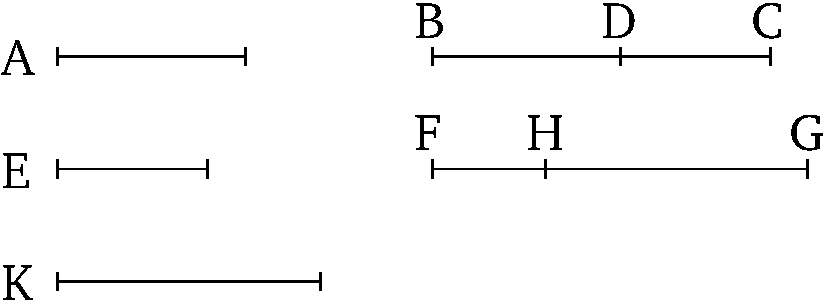
\includegraphics{Book10/fig090e.pdf}}

Therefore, since as $E$ is to $BC$, so the (square) on $A$ (is)
to the (square) on $FG$, the (square) on $A$ (is) thus commensurable
with the (square) on $FG$ [Prop.~10.6]. 
And the (square) on $A$ (is) rational. Thus, the (square) on $FG$
(is) also rational. Thus, $FG$  is also a rational (straight-line). And
since $E$ does not have to $BC$ the ratio which (some) square
number (has) to (some) square number, the (square) on $A$
thus does not have to the (square) on $FG$ the ratio which (some)
square number (has) to (some) square number either. Thus,
$A$ is incommensurable in length with $FG$ [Prop.~10.9]. Again, since as $BC$ is to $CD$, so
the (square) on $FG$ (is) to the (square) on $GH$, the (square) on
$FG$ (is) thus commensurable with the (square) on $GH$ [Prop.~10.6]. And the (square) on $FG$ (is) rational.
Thus, the (square) on $GH$ (is) also rational. Thus, $GH$
(is) also rational. And since $BC$ does not have to $CD$ the ratio
which (some) square number (has) to (some) square number, the
(square) on $FG$ thus does not have to the (square) on $GH$
the ratio which (some) square (number) has to (some) square (number)
either. Thus, $FG$ is incommensurable in length with $GH$ [Prop.~10.9]. And both are rational (straight-lines).
Thus, $FG$ and $GH$ are rational (straight-lines which are) commensurable
in square only. Thus, $FH$ is an apotome [Prop.~10.73]. So, I say that (it is) also a sixth (apotome).

For since as $E$ is to $BC$, so the (square) on $A$ (is) to the (square)
on $FG$, and as $BC$ (is) to $CD$, so the (square) on $FG$ (is) to
the (square) on $GH$, thus, via equality, as $E$ is to $CD$, so the
(square) on $A$ (is) to the (square) on $GH$ [Prop.~5.22]. And $E$ does not have to $CD$
the ratio which (some) square number (has) to (some) square number.
Thus, the (square) on $A$ does not have to the (square) $GH$ the
ratio which (some) square number (has) to (some) square number either. $A$ is thus incommensurable in length with $GH$ [Prop.~10.9]. Thus, neither of $FG$ and $GH$
is commensurable in length with the rational (straight-line) $A$. Therefore, let the (square)
on $K$ be that (area) by which the (square) on $FG$ is greater than the (square) on $GH$ [Prop.~10.13~lem.].
 Therefore, since as $BC$ is to $CD$, so the (square) on $FG$ (is) to the
(square) on $GH$, thus, via conversion, as $CB$ is to $BD$, so the (square)
on $FG$ (is) to the (square) on $K$ [Prop.~5.19~corr.]. And $CB$ does not have
to $BD$ the ratio which (some) square number (has) to (some) square
number. Thus, the (square) on $FG$ does not have to the (square) on
$K$ the ratio which (some) square number (has) to (some) square number
either. $FG$ is thus incommensurable in length with $K$ [Prop.~10.9]. And the square on $FG$ is greater
than (the square on) $GH$ by the (square) on $K$.
Thus, the square on
$FG$ is greater than (the square on) $GH$ by the (square)
on (some straight-line) incommensurable in length with ($FG$).
And neither of $FG$ and $GH$ is commensurable in length
with the (previously) laid down rational (straight-line) $A$. Thus,
$FH$ is a sixth apotome [Def.~10.16].

Thus, the sixth apotome $FH$ has been found. (Which is) the
very thing it was required to show.}
\end{Parallel}
{\footnotesize\noindent$^\dag$ See footnote to Prop.~10.53.}

%%%%
%10.91
%%%%
\pdfbookmark[1]{Proposition 10.91}{pdf10.91}
\begin{Parallel}{}{}
\ParallelLText{
\begin{center}
{\large \ggn{91}.}
\end{center}\vspace*{-7pt}

\gr{Ἐὰν θωρίον περιέθηται ὑπὸ <ρητῆξ καὶ ἀποτομ\kern -.7pt  ῆξ πρώτηξ,
ἡ τὸ θωρίον δυναμένη ἀπορομ\kern -.7pt  ή ἐστιν.}

\gr{Περιεθέσθω γὰρ θωρίον τὸ ΑΒ ὑπὸ <ρητῆξ τῆξ ΑΓ καὶ ἀποτομ\kern -.7pt  ῆξ
πρώτηξ τῆξ ΑΔ; λέγω, <ότι ἡ τὸ ΑΒ θωρίον δυναμένη ἀποτομ\kern -.7pt  ή
ἐστιν.}

\gr{Ἐπεὶ γὰρ ἀποτομ\kern -.7pt  ή ἐστι πρώτη ἡ ΑΔ, >έστω α\kern -.7pt  ὐτῆ| προσαρμόζουσα
ἡ ΔΗ; αἱ ΑΗ, ΗΔ >άρα <ρηταί εἰσι δυνάμει μόνον σύμμετροι.
καὶ <όλη ἡ ΑΗ σύμμετρόξ ἐστι τῆ| ἐκκειμένῃ <ρητῆ| τῆ| ΑΓ,
καὶ ἡ ΑΗ τῆξ ΗΔ μεῖζον δύναται τῶ| ἀπὸ συμμέτρου ἑαυτῆ|
μ\kern -.5pt  ήκει; ἒαν >άρα τῶ| τετάρτῳ μέρει τοῦ ἀπὸ τῆξ ΔΗ >ίσον
παρὰ τὴν ΑΗ παραβληθῆ| ἐλλεῖπον ε>ίδει τετραγώνῳ, εἰξ σύμμετρα
α\kern -.3pt  ὐτὴν διαιρεῖ. τετμ\kern -.7pt  ήσθω ἡ ΔΗ δίθα κατὰ τὸ Ε, καὶ τῶ| ἀπὸ
τῆξ ΕΗ >ίσον παρὰ τὴν ΑΗ παραβεβλήσθω ἐλλεῖπον ε>ίδει
τετραγώνῳ, καὶ >έστω τὸ ὑπὸ τῶν ΑΖ, ΖΗ; σύμμετροξ >άρα
ἐστὶν ἡ ΑΖ τῆ| ΖΗ. καὶ διὰ τῶν Ε, Ζ, Η σημείων τῆ| ΑΓ
παράλληλοι >ήθθωσαν αἱ ΕΘ, ΖΙ, ΗΚ.}\\~\\~\\~\\~\\

% Removed epsf size command
\centerline{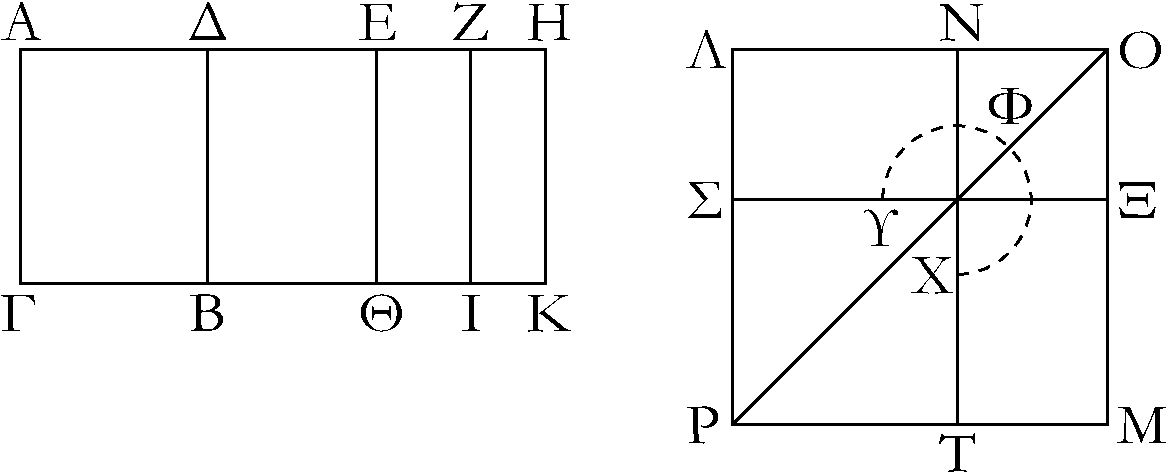
\includegraphics{Book10/fig091g.pdf}}


\gr{Καὶ ἐπεὶ σύμμετρόξ ἐστιν ἡ ΑΖ τῆ| ΖΗ μ\kern -.7pt  ήκει, καὶ ἡ ΑΗ
>άρα ἑκατέρᾳ τῶν ΑΖ, ΖΗ σύμμετρόξ ἐστι μ\kern -.7pt  ήκει. ἀλλὰ
ἡ ΑΗ σύμμετρόξ ἐστι τῆ| ΑΓ; καὶ ἑκατέρα
>άρα τῶν ΑΖ, ΖΗ σύμμετρόξ ἐστι τῆ| ΑΓ μ\kern -.5pt  ήκει. καί ἐστι
<ρητὴ ἡ ΑΓ; <ρητὴ >άρα καὶ ἑκατέρα τῶν ΑΖ, ΖΗ; <ώστε καὶ
ἑκάτερον τῶν ΑΙ, ΖΚ <ρητόν ἐστιν. καὶ ἐπεὶ σύμμετρόξ
ἐστιν ἡ ΔΕ τῆ| ΕΗ μ\kern -.3pt  ήκει, καὶ ἡ ΔΗ >άρα ἑκατέρᾳ τῶν
ΔΕ, ΕΗ σύμμετρόξ ἐστι μ\kern -.7pt  ήκει. <ρητὴ δὲ ἡ ΔΗ καὶ
ἀσύμμετροξ τῆ| ΑΓ μ\kern -.7pt  ήκει; <ρητὴ >άρα καὶ ἑκατέρα τῶν
ΔΕ, ΕΗ καὶ ἀσύμμετροξ τῆ| ΑΓ μ\kern -.7pt  ήκει; ἑκάτερον >άρα τῶν
ΔΘ, ΕΚ μέσον ἐστίν.}

\gr{Κείσθω δὴ τῶ| μὲν ΑΙ >ίσον τετράγωνον τὸ ΛΜ,
τῶ| δὲ ΖΚ >ίσον τετράγωνον ἀφῃρήσθω κοινὴν γωνίαν
>έθον α\kern -.7pt  ὐτῶ| τὴν ὑπὸ ΛΟΜ τὸ ΝΧ; περὶ τὴν
α\kern -.7pt  ὐτὴν >άρα διάμετρόν ἐστι τὰ ΛΜ, ΝΧ τετράγωνα. >έστω
α\kern -.5pt  ὐτῶν διάμετροξ ἡ ΟΡ, καὶ καταγεγράφθω τὸ σθῆμα.
ἐπεὶ ο>ῦν >ίσον ἐστὶ τὸ ὑπὸ τῶν ΑΖ, ΖΗ περιεχόμενον ὀρθογώνιον τῶ| ἀπὸ τῆξ ΕΗ τετραγώνῳ, >έστιν >άρα ὡξ
ἡ ΑΖ πρὸξ τὴν ΕΗ, ο<ύτωξ ἡ ΕΗ πρὸξ τὴν ΖΗ.
ἀλλ> ὡξ μὲν ἡ ΑΖ πρὸξ τὴν ΕΗ, ο<ύτωξ τὸ ΑΙ πρὸξ
τὸ ΕΚ, ὡξ δὲ ἡ ΕΗ πρὸξ τὴν ΖΗ, ο<ύτωξ ἐστὶ τὸ ΕΚ πρὸξ
τὸ ΚΖ; τῶν >άρα ΑΙ, ΚΖ μέσον ἀνάλογόν ἐστι τὸ ΕΚ. >έστι
δὲ καὶ τῶν ΛΜ, ΝΧ μέσον ἀνάλογον τὸ ΜΝ,  ὡξ
ἐν τοῖξ >έμπροσθεν ἐδείθθη, καί ἐστι τὸ [μὲν] ΑΙ τῶ| ΛΜ
τετραγώνῳ >ίσον, τὸ δὲ ΚΖ τῶ| ΝΧ; καὶ τὸ ΜΝ >άρα τῶ| ΕΚ >ίσον
 ἐστίν. ἀλλὰ τὸ μὲν ΕΚ τῶ| ΔΘ ἐστιν >ίσον,
τὸ δὲ ΜΝ τῶ| ΛΧ; τὸ >άρα ΔΚ >ίσον ἐστὶ τῶ| ΥΦΘ γνώμονι
καὶ τῶ| ΝΧ. >έστι δὲ καὶ τὸ ΑΚ >ίσον τοῖξ ΛΜ, ΝΧ τετραγώνοιξ;
λοιπὸν >άρα τὸ ΑΒ >ίσον ἐστὶ τῶ| ΣΤ. τὸ δὲ ΣΤ τὸ ἀπὸ
τῆξ ΛΝ ἐστι τετράγωνον; τὸ >άρα ἀπὸ τῆξ ΛΝ τετράγωνον >ίσον
ἐστὶ τῶ| ΑΒ; ἡ ΛΝ >άρα δύναται τὸ ΑΒ. λέγω δή, <ότι
ἡ ΛΝ ἀποτομ\kern -.3pt  ή ἐστιν.}

\gr{Ἐπεὶ γὰρ <ρητόν ἐστιν ἑκάτερον τῶν ΑΙ, ΖΚ, καί ἐστιν >ίσον
τοῖξ ΛΜ, ΝΧ, καὶ ἑκάτερον >άρα τῶν ΛΜ, ΝΧ <ρητόν ἐστιν,
τουτέστι τὸ ἀπὸ ἑκατέραξ τῶν ΛΟ, ΟΝ; καὶ ἑκατέρα >άρα τῶν
ΛΟ, ΟΝ <ρητή ἐστιν. πάλιν, ἐπεὶ μέσον ἐστὶ τὸ ΔΘ καί ἐστιν
>ίσον τῶ| ΛΧ, μέσον >άρα ἐστὶ καὶ τὸ ΛΧ. ἐπεὶ ο>ῦν τὸ μὲν
ΛΧ μέσον ἐστίν, τὸ δὲ ΝΧ <ρητόν, ἀσύμμετρον >άρα ἐστὶ
τὸ ΛΧ τῶ| ΝΧ; ὡξ δὲ τὸ ΛΧ πρὸξ τὸ ΝΧ, ο<ύτωξ
ἐστὶν ἡ ΛΟ πρὸξ τὴν ΟΝ; ἀσύμμετροξ >άρα ἐστὶν ἡ  ΛΟ
τῆ| ΟΝ μ\kern -.7pt  ήκει. καί εἰσιν ἀμφότεραι <ρηταί; αἱ ΛΟ, ΟΝ >άρα
<ρηταί εἰσι δυνάμει μόνον σύμμετροι; ἀποτομ\kern -.7pt  ὴ
>άρα ἐστὶν ἡ ΛΝ. καὶ δύναται τὸ ΑΒ θωρίον;
ἡ >άρα τὸ ΑΒ θωρίον δυναμένη ἀποτομ\kern -.5pt  ή ἐστιν.}

\gr{Ἐὰν >άρα θωρίον περιέθηται ὑπὸ <ρητῆξ καὶ τὰ
ἑχῆξ.}}

\ParallelRText{
\begin{center}
{\large Proposition 91}
\end{center}

If an area is contained by a rational (straight-line)
and a first apotome then the square-root of the area is an apotome.

For let the area $AB$ be contained by the rational (straight-line) $AC$ and the first apotome $AD$. I say that the square-root of area $AB$ is an apotome.

For since $AD$ is a first apotome, let $DG$ be its attachment. Thus,
$AG$ and $DG$ are rational (straight-lines which are) commensurable in
square only [Prop.~10.73]. And the whole, $AG$,
is commensurable (in length) with the (previously) laid down rational (straight-line)
$AC$, and the square on $AG$ is greater than (the square on) $GD$
by the (square) on  (some straight-line) commensurable in length with ($AG$) [Def.~10.11]. Thus, if (an area) equal to the
fourth part of the (square) on $DG$ is applied to $AG$, falling short
by a square figure, then it divides ($AG$) into (parts which are) commensurable
(in length) [Prop.~10.17]. Let $DG$
be cut in half at $E$. And let (an area) equal to the (square) on
$EG$ be applied to $AG$, falling short by a square figure. And let
it be the (rectangle contained) by $AF$ and $FG$. $AF$ is
 thus commensurable (in length) with $FG$. And let $EH$, $FI$, and $GK$
be drawn through points $E$, $F$, and $G$ (respectively),
parallel to $AC$.

% Removed epsf size command
\centerline{\includegraphics{Book10/fig091e.pdf}}

And since $AF$ is commensurable in length with $FG$, $AG$ is thus also
commensurable in length with each of $AF$ and $FG$ [Prop.~10.15]. But $AG$ is commensurable (in length)
with $AC$. Thus, each of $AF$ and $FG$ is also commensurable in length with $AC$ 
[Prop.~10.12]. 
And $AC$ is a rational (straight-line). Thus,  $AF$ and $FG$ (are) each
also rational (straight-lines). Hence, $AI$ and
$FK$ are also each rational (areas) [Prop.~10.19]. And since $DE$ is commensurable
in length with $EG$, $DG$ is thus also commensurable
in length with each of $DE$ and $EG$ [Prop.~10.15]. And $DG$ (is) rational, and
incommensurable in length with $AC$. $DE$ and $EG$ (are) thus each
rational, and incommensurable in length with $AC$ [Prop.~10.13]. Thus, $DH$ and $EK$ are
each medial (areas) [Prop.~10.21].

So let the square $LM$, equal to $AI$, be laid down. And let the square $NO$,
equal to $FK$, be
subtracted (from $LM$), having with it the common angle $LPM$. Thus,
the squares $LM$ and $NO$ are about the same diagonal [Prop.~6.26]. Let $PR$ be their (common) diagonal, and
let the (rest of the) figure be drawn. Therefore, since
the rectangle contained by $AF$ and $FG$ is equal to the square $EG$,
thus as $AF$ is to $EG$, so $EG$ (is) to $FG$ [Prop.~6.17]. But, as $AF$ (is) to $EG$, so $AI$ (is)
to $EK$, and as $EG$ (is) to $FG$, so $EK$ is to $KF$ [Prop.~6.1]. Thus, $EK$ is the mean proportional
to $AI$ and $KF$ [Prop.~5.11]. And $MN$ is also the mean proportional to
$LM$ and $NO$, as shown before [Prop.~10.53~lem.].  And $AI$ is equal to the
square $LM$, and $KF$ to $NO$. Thus, $MN$ is also equal to $EK$.
But, $EK$ is equal to $DH$, and $MN$ to $LO$ [Prop.~1.43]. Thus, $DK$ is equal to the
gnomon $UVW$ and  $NO$. And $AK$ is also equal to 
(the sum of) the squares $LM$ and $NO$.  Thus, the remainder $AB$ is equal
to $ST$. And $ST$ is the square on $LN$. Thus, the square on $LN$
is equal to $AB$. Thus, $LN$ is the square-root of $AB$. So, I say that
$LN$ is an apotome.

For since $AI$ and $FK$ are each rational (areas), and are equal to
$LM$ and $NO$ (respectively), thus  $LM$ and $NO$---that is to say, the
(squares) on each of $LP$ and $PN$ (respectively)---are  also
each rational (areas). Thus, $LP$ and $PN$ are also each rational (straight-lines). 
Again, since $DH$ is a medial (area), and is equal to $LO$, $LO$ is thus
also a medial (area). Therefore, since $LO$ is medial, and $NO$ rational, 
$LO$ is thus incommensurable with $NO$. And as $LO$ (is) to $NO$,
so $LP$ is to $PN$ [Prop.~6.1]. $LP$ is
thus incommensurable in length with $PN$ [Prop.~10.11]. And they are both rational
(straight-lines). Thus, $LP$ and $PN$ are rational (straight-lines which are)
commensurable in square only. Thus, $LN$ is an apotome [Prop.~10.73]. And it is the square-root of area $AB$. Thus, the square-root of area $AB$ is an apotome.

Thus, if an area is contained by a rational (straight-line), and
so on \ldots.}
\end{Parallel}

%%%%
%10.92
%%%%
\pdfbookmark[1]{Proposition 10.92}{pdf10.92}
\begin{Parallel}{}{}
\ParallelLText{
\begin{center}
{\large \ggn{92}.}
\end{center}\vspace*{-7pt}

\gr{Ἐὰν θωρίον περιέθηται ὑπὸ <ρητῆξ καὶ ἀποτομ\kern -.7pt  ῆξ δευτέραξ,
ἡ τὸ θωρίον δυναμένη μέσηξ ἀποτομ\kern -.7pt  ή ἐστι πρώτη.}\\

% Removed epsf size command
\centerline{\includegraphics{Book10/fig092g.pdf}}

\gr{Θωρίον γὰρ τὸ ΑΒ περιεθέσθω ὑπὸ <ρητῆξ τῆξ ΑΓ καὶ ἀποτομ\kern -.7pt  ῆξ
δευτέραξ τῆξ ΑΔ; λέγω, <ότι ἡ τὸ ΑΒ θωρίον δυναμένη μέσηξ
ἀποτομ\kern -.7pt  ή ἐστι πρώτη.}

\gr{>'Εστω γὰρ τῆ| ΑΔ προσαρμόζουσα ἡ ΔΗ; αἱ >άρα ΑΗ, ΗΔ
<ρηταί εἰσι δυνάμει μόνον σύμμετροι, καὶ ἡ προσαρμόζουσα
ἡ ΔΗ σύμμετρόξ ἐστι τῆ| ἐκκειμένῃ
<ρητῆ| τῆ| ΑΓ, ἡ δὲ <όλη ἡ ΑΗ τῆξ προσαρμοζούσηξ τῆξ
ΗΔ μεῖζον δύναται τῶ| ἀπὸ συμμέτρου ἑαυτῆ| μ\kern -.7pt  ήκει.
ἐπεὶ ο>ῦν ἡ ΑΗ τῆξ ΗΔ μεῖζον δύναται τῶ| ἀπὸ
συμμέτρου ἑαυτῆ|, ἒαν >άρα τῶ| τετάρτῳ μέρει τοῦ ἀπὸ τῆξ
ΗΔ >ίσον παρὰ τὴν ΑΗ παραβληθῆ| ἐλλεῖπον ε>ίδει
τετραγώνῳ, εἰξ σύμμετρα α\kern -.7pt  ὐτὴν διαιρεῖ. τετμ\kern -.5pt  ήσθω ο>ῦν ἡ
ΔΗ δίθα κατὰ τὸ Ε; καὶ τῶ| ἀπὸ τῆξ ΕΗ >ίσον παρὰ τὴν ΑΗ
παραβεβλήσθω ἐλλεῖπον ε>ίδει τετραγώνῳ, καὶ >έστω τὸ ὑπὸ
τῶν ΑΖ, ΖΗ; σύμμετροξ >άρα ἐστὶν ἡ ΑΖ τῆ| ΖΗ μ\kern -.3pt  ήκει. καὶ
ἡ ΑΗ >άρα ἑκατέρᾳ τῶν ΑΖ, ΖΗ σύμμετρόξ ἐστι μ\kern -.7pt  ήκει.
<ρητὴ δὲ ἡ ΑΗ καὶ ἀσύμμετροξ τῆ| ΑΓ μ\kern -.7pt  ήκει; καὶ ἑκατέρα
>άρα τῶν ΑΖ, ΖΗ <ρητή ἐστι καὶ ἀσύμμετροξ τῆ| ΑΓ μ\kern -.7pt  ήκει;
ἑκάτερον >άρα τῶν ΑΙ, ΖΚ μέσον ἐστίν. πάλιν, ἐπεὶ
σύμμετρόξ ἐστιν ἡ ΔΕ τῆ| ΕΗ, καὶ ἡ ΔΗ >άρα ἑκατέρᾳ τῶν
ΔΕ, ΕΗ σύμμετρόξ ἐστιν. ἀλλ> ἡ ΔΗ σύμμετρόξ ἐστι τῆ|
ΑΓ μ\kern -.7pt  ήκει [<ρητὴ >άρα καὶ ἑκατέρα τῶν ΔΕ, ΕΗ καὶ σύμμετροξ
τῆ| ΑΓ μ\kern -.7pt  ήκει]. ἑκάτερον >άρα τῶν ΔΘ, ΕΚ <ρητόν ἐστιν.}

\gr{Συνεστάτω ο>ῦν τῶ| μὲν ΑΙ >ίσον τετράγωνον τὸ ΛΜ, τῶ|
δὲ ΖΚ >ίσον ἀφῃρήσθω τὸ ΝΧ περὶ τὴν α\kern -.7pt  ὐτὴν γωνίαν >ὸν
τῶ| ΛΜ τὴν ὑπὸ τῶν ΛΟΜ; περὶ τὴν α\kern -.7pt  ὐτὴν >άρα ἐστὶ
διάμετρον τὰ ΛΜ, ΝΧ τετράγωνα. >έστω α\kern -.5pt  ὐτῶν διάμετροξ
ἡ ΟΡ, καὶ καταγεγράφθω τὸ σθῆμα. ἐπεὶ ο>ῦν τὰ ΑΙ, ΖΚ μέσα
ἐστὶ καί ἐστιν >ίσα τοῖξ ἀπὸ τῶν ΛΟ, ΟΝ, καὶ τὰ ἀπὸ τῶν
ΛΟ, ΟΝ [>άρα] μέσα ἐστίν; καὶ αἱ ΛΟ, ΟΝ >άρα μέσαι εἰσὶ
δυνάμει μόνον σύμμετροι. καὶ ἐπεὶ τὸ ὑπὸ τῶν ΑΖ,
ΖΗ >ίσον ἐστὶ τῶ| ἀπὸ τῆξ ΕΗ, >έστιν >άρα ὡξ ἡ ΑΖ πρὸξ
τὴν ΕΗ, ο<ύτωξ ἡ ΕΗ πρὸξ τὴν ΖΗ; ἀλλ> ὡξ μὲν ἡ ΑΖ
πρὸξ τὴν ΕΗ, ο<ύτωξ τὸ ΑΙ πρὸξ τὸ ΕΚ; ὡξ δὲ ἡ ΕΗ πρὸξ τὴν
ΖΗ, ο<ύτωξ [ἐστὶ] τὸ ΕΚ πρὸξ τὸ ΖΚ; τῶν >άρα ΑΙ, ΖΚ μέσον
ἀνάλογόν ἐστι τὸ ΕΚ. >έστι δὲ καὶ τῶν ΛΜ, ΝΧ τετραγώνων
μέσον ἀνάλογον τὸ ΜΝ; καί ἐστιν >ίσον τὸ μὲν ΑΙ τῶ| ΛΜ,
τὸ δὲ ΖΚ τῶ| ΝΧ;  καὶ  τὸ ΜΝ >άρα >ίσον ἐστὶ τῶ| ΕΚ. ἀλλὰ
τῶ| μὲν ΕΚ >ίσον [ἐστὶ] τὸ ΔΘ, τῶ| δὲ ΜΝ >ίσον τὸ ΛΧ; <όλον
>άρα τὸ ΔΚ >ίσον ἐστὶ τῶ| ΥΦΘ γνώμονι καὶ τῶ| ΝΧ. ἐπεὶ
ο>ῦν <όλον τὸ ΑΚ >ίσον ἐστὶ τοῖξ ΛΜ, ΝΧ, <ῶν τὸ ΔΚ
>ίσον ἐστὶ τῶ| ΥΦΘ γνώμονι καὶ τῶ| ΝΧ, λοιπὸν >άρα τὸ ΑΒ
>ίσον ἐστὶ τῶ| ΤΣ. τὸ δὲ ΤΣ ἐστι τὸ ἀπὸ τῆξ ΛΝ;
τὸ ἀπὸ τῆξ ΛΝ >άρα >ίσον ἐστὶ τῶ| ΑΒ θωρίῳ; ἡ ΛΝ
>άρα δύναται τὸ ΑΒ θωρίον. λέγω [δή], <ότι ἡ ΛΝ μέσηξ
ἀποτομ\kern -.3pt  ή ἐστι πρώτη.}

\gr{Ἐπεὶ γὰρ <ρητόν ἐστι τὸ ΕΚ καί ἐστιν >ίσον τῶ| ΛΧ,
<ρητὸν >άρα ἐστὶ τὸ ΛΧ, τουτέστι τὸ ὑπὸ τῶν
ΛΟ, ΟΝ. μέσον δὲ ἐδείθθη τὸ ΝΧ; ἀσύμμετρον >άρα
ἐστὶ τὸ ΛΧ τῶ| ΝΧ; ὡξ δὲ τὸ ΛΧ πρὸξ τὸ ΝΧ,
ο<ύτωξ ἐστὶν ἡ ΛΟ πρὸξ ΟΝ; αἱ ΛΟ, ΟΝ >άρα ἀσύμμετροί
εἰσι μ\kern -.7pt  ήκει. αἱ >άρα ΛΟ, ΟΝ μέσαι εἰσὶ δυνάμει μόνον σύμμετροι
<ρητὸν περιέθουσαι; ἡ ΛΝ >άρα μέσηξ ἀποτομ\kern -.7pt  ή ἐστι πρώτη;
καὶ δύναται τὸ ΑΒ θωρίον.}

\gr{Ἡ >άρα τὸ ΑΒ θωρίον δυναμένη μέσηξ ἀποτομ\kern -.7pt  ή ἐστι
πρώτη; <όπερ >έδει δεῖχαι.}}

\ParallelRText{
\begin{center}
{\large Proposition 92}
\end{center}

If an area is contained by a rational (straight-line)
and a second apotome then the square-root of the area is a first apotome of a medial (straight-line).

% Removed epsf size command
\centerline{\includegraphics{Book10/fig092e.pdf}}

For let the area $AB$ be contained by the rational (straight-line) $AC$ and the second apotome $AD$. I say that the square-root of area $AB$ is the first apotome of a medial (straight-line).

For let $DG$ be an attachment to $AD$. Thus, $AG$ and $GD$
are rational (straight-lines which are) commensurable in square only [Prop.~10.73],
and the attachment $DG$ is commensurable (in length) with the
(previously) laid down rational (straight-line) $AC$, and the square on
the whole, $AG$, is greater than (the square on) the attachment, $GD$,
by the (square) on (some straight-line) commensurable in length with ($AG$) 
[Def.~10.12]. Therefore, since the square on $AG$ is
greater than (the square on) $GD$ by the (square) on (some
straight-line) commensurable (in length) with ($AG$), thus if  (an area)
equal to the fourth part of the (square) on $GD$ is applied
to $AG$, falling short by a square figure, then it divides ($AG$) into (parts which
are) commensurable (in length) [Prop.~10.17]. 
Therefore, let $DG$ be cut in half at $E$. And let (an area) equal to
the (square) on $EG$ be applied to $AG$, falling short
by a square figure. And let it be the (rectangle contained) by $AF$ and $FG$.
Thus, $AF$ is commensurable in length with $FG$. $AG$ is thus
also commensurable in length with each of $AF$ and $FG$ [Prop.~10.15]. And $AG$ (is) a rational (straight-line), and incommensurable in length with $AC$. $AF$ and $FG$
are thus also each rational (straight-lines), and incommensurable in length with
$AC$ [Prop.~10.13].
Thus, $AI$
and $FK$ are each medial (areas) [Prop.~10.21]. 
Again, since $DE$ is commensurable (in length) with $EG$, thus
$DG$ is also commensurable (in length) with each of $DE$ and $EG$ [Prop.~10.15]. But, $DG$ is commensurable
in length with $AC$ [thus, $DE$ and $EG$ are also each rational, and
commensurable in length with $AC$]. Thus, $DH$ and $EK$ are each
rational (areas) [Prop.~10.19].

Therefore, let the square $LM$, equal to $AI$, be constructed.
And let $NO$, equal to $FK$, which is about the
same angle $LPM$ as $LM$, be subtracted (from $LM$).
Thus, the squares $LM$ and $NO$ are about the same diagonal
[Prop.~6.26]. Let $PR$ be their (common) diagonal, and
let the (rest of the) figure be drawn. Therefore, since $AI$ and $FK$
are medial (areas), and are equal to the (squares) on $LP$ and $PN$
(respectively), [thus] the (squares) on $LP$ and $PN$ are also medial.
Thus, $LP$ and $PN$ are  also medial (straight-lines which are)
commensurable in square only.$^\dag$ And since the (rectangle contained) by
$AF$ and $FG$ is equal to the (square) on $EG$, thus as $AF$ is to $EG$, so $EG$ (is) to $FG$ [Prop.~10.17]. But, as
$AF$ (is) to $EG$, so $AI$ (is) to $EK$. And as $EG$ (is) to $FG$, so
$EK$ [is] to $FK$ [Prop.~6.1]. Thus, $EK$ is the mean proportional to $AI$ and $FK$ [Prop.~5.11].
And $MN$ is also the mean proportional to the squares $LM$ and $NO$ [Prop.~10.53~lem.]. 
And $AI$ is equal to $LM$, and $FK$ to $NO$. 
Thus, $MN$ is also equal to
$EK$. But, $DH$ [is] equal to $EK$, and $LO$ equal to $MN$ [Prop.~1.43]. Thus, the whole  (of) $DK$ is equal to
the gnomon $UVW$ and $NO$. Therefore, since the whole (of) $AK$
is equal to $LM$ and $NO$, of which $DK$ is equal to the
gnomon $UVW$ and $NO$,  the remainder $AB$ is thus equal to $TS$.
And $TS$ is the (square) on $LN$. Thus, the (square) on $LN$
is equal to the area $AB$. $LN$ is thus the square-root of area $AB$.
[So], I say that $LN$ is the first apotome of a medial (straight-line).

For since $EK$ is a rational (area), and is equal to $LO$, $LO$---that is to
say, the (rectangle contained) by $LP$ and $PN$---is thus
a rational (area). And $NO$ was shown (to be) a medial (area). Thus,
$LO$ is incommensurable  with $NO$. And as $LO$ (is) to $NO$,
so $LP$ is to $PN$ [Prop.~6.1]. Thus,  $LP$ and
$PN$ are incommensurable in length [Prop.~10.11]. 
$LP$ and $PN$ are thus medial (straight-lines which are) commensurable
in square only, and which contain a rational (area). Thus, $LN$ is the
first apotome of a medial (straight-line) [Prop.~10.74]. And it is the square-root of area $AB$.

Thus, the square root of area $AB$ is the first apotome of a medial (straight-line). (Which is) the very thing it was required to show.}
\end{Parallel}
{\footnotesize\noindent$^\dag$ There is an error in the argument here. It should just say that $LP$ and $PN$ are commensurable in square,
rather than in square only, since $LP$ and $PN$ are only shown
to be incommensurable in length later on.}

%%%%
%10.93
%%%%
\pdfbookmark[1]{Proposition 10.93}{pdf10.93}
\begin{Parallel}{}{}
\ParallelLText{
\begin{center}
{\large \ggn{93}.}
\end{center}\vspace*{-7pt}

\gr{Ἐὰν θωρίον περιέθηται ὑπὸ <ρητῆξ καὶ ἀποτομ\kern -.7pt  ῆξ τρίτηξ,
ἡ τὸ θωρίον δυναμένη μέσηξ ἀποτομ\kern -.7pt  ή ἐστι δευτέρα.}

\gr{Θωρίον γὰρ τὸ ΑΒ περιεθέσθω ὑπὸ <ρητῆξ τῆξ ΑΓ καὶ ἀποτομ\kern -.7pt  ῆξ
τρίτηξ τῆξ ΑΔ; λέγω, <ότι ἡ τὸ ΑΒ θωρίον δυναμένη μέσηξ
ἀποτομ\kern -.7pt  ή ἐστι δευτέρα.}\\

% Removed epsf size command
\centerline{\includegraphics{Book10/fig093g.pdf}}

\gr{>'Εστω γὰρ τῆ| ΑΔ προσαρμόζουσα ἡ ΔΗ; αἱ ΑΗ, ΗΔ >άρα <ρηταί εἰσι
δυνάμει μόνον σύμμετροι, καὶ οὐδετέρα τῶν ΑΗ, ΗΔ σύμμετρόξ
ἐστι μ\kern -.7pt  ήκει τῆ| ἐκκειμένῃ <ρητῆ| τῆ| ΑΓ, ἡ δὲ <όλη ἡ ΑΗ
τὴξ προσαρμοζούσηξ τῆξ ΔΗ μεῖζον δύναται τῶ| ἀπὸ
συμμέτρου ἑαυτῆ|. ἐπεὶ ο>ῦν ἡ ΑΗ τῆξ ΗΔ μεῖζον
δύναται τῶ| ἀπὸ συμμέτρου ἑαυτῆ|, ἒαν >άρα τῶ| τετάρτῳ
μέρει τοῦ ἀπὸ τῆξ ΔΗ >ίσον παρὰ τὴν ΑΗ παραβληθῆ| ἐλλεῖπον
ε>ίδει τετραγώνῳ, εἰξ σύμμετρα α\kern -.7pt  ὐτὴν διελεῖ. τετμ\kern -.5pt  ήσθω
ο>ῦν ἡ ΔΗ δίθα κατὰ τὸ Ε, καὶ τῶ| ἀπὸ τῆξ ΕΗ >ίσον
παρὰ τὴν ΑΗ παραβεβλήσθω ἐλλεῖπον ε>ίδει τετραγώνῳ, καὶ
>έστω τὸ ὑπὸ τῶν ΑΖ, ΖΗ. καὶ >ήθθωσαν διὰ τῶν Ε, Ζ, Η σημείων
τῆ| ΑΓ παράλληλοι αἱ ΕΘ, ΖΙ, ΗΚ; σύμμετροι >άρα εἰσὶν αἱ ΑΖ, ΖΗ;
σύμμετρον >άρα καὶ τὸ ΑΙ τῶ| ΖΚ. καὶ ἐπεὶ αἱ ΑΖ, ΖΗ σύμμετροί
εἰσι μ\kern -.3pt  ήκει, καὶ ἡ ΑΗ >άρα ἑκατέρᾳ τῶν ΑΖ, ΖΗ σύμμετρόξ
ἐστι μ\kern -.7pt  ήκει. <ρητὴ δὲ ἡ ΑΗ καὶ ἀσύμμετροξ τῆ| ΑΓ μ\kern -.7pt  ήκει; <ώστε
καὶ αἱ ΑΖ, ΖΗ. ἑκάτερον >άρα τῶν ΑΙ, ΖΚ μέσον ἐστίν. πάλιν, ἐπεὶ
σύμμετρόξ ἐστιν ἡ ΔΕ τῆ| ΕΗ μ\kern -.7pt  ήκει, καὶ ἡ ΔΗ >άρα ἑκατέρᾳ
τῶν ΔΕ, ΕΗ σύμμετρόξ ἐστι μ\kern -.7pt  ήκει. <ρητὴ δὲ ἡ ΗΔ καὶ
ἀσύμμετροξ τῆ| ΑΓ μ\kern -.7pt  ήκει; <ρητὴ >άρα καὶ ἑκατέρα τῶν ΔΕ,
ΕΗ καὶ ἀσύμμετροξ τῆ| ΑΓ μ\kern -.7pt  ήκει; ἑκάτερον >άρα τῶν ΔΘ, ΕΚ
μέσον ἐστίν. καὶ ἐπεὶ αἱ ΑΗ, ΗΔ δυνάμει μόνον σύμμετροί
εἰσιν, ἀσύμμετροξ >άρα ἐστὶ μ\kern -.7pt  ήκει ἡ ΑΗ τῆ| ΗΔ. ἀλλ>
ἡ μὲν ΑΗ τῆ| ΑΖ σύμμετρόξ ἐστι μ\kern -.7pt  ήκει ἡ δὲ ΔΗ τῆ| ΕΗ;
ἀσύμμετροξ >άρα ἐστὶν ἡ ΑΖ τῆ| ΕΗ μ\kern -.7pt  ήκει. ὡξ δὲ ἡ ΑΖ
πρὸξ τὴν ΕΗ, ο<ύτωξ ἐστὶ τὸ ΑΙ πρὸξ τὸ ΕΚ;
ἀσύμμετρον >άρα ἐστὶ τὸ ΑΙ τῶ| ΕΚ.}

\gr{Συνεστάτω ο>ῦν τῶ| μὲν ΑΙ >ίσον τετράγωνον τὸ ΛΜ, τῶ| δὲ
ΖΚ >ίσον ἀφῆ|ρήσθω τὸ ΝΧ περὶ τὴν α\kern -.7pt  ὐτὴν γωνίαν >ὸν τῶ|
ΛΜ; περὶ τὴν α\kern -.7pt  ὐτὴν >άρα διάμετρόν ἐστι τὰ ΛΜ, ΝΧ. >έστω
α\kern -.5pt  ὐτῶν διάμετροξ ἡ ΟΡ, καὶ καταγεγράφθω τὸ σθῆμα. ἐπεὶ
ο>ῦν τὸ ὑπὸ τῶν ΑΖ, ΖΗ >ίσον ἐστὶ τῶ| ἀπὸ τῆξ ΕΗ,
>έστιν >άρα ὡξ ἡ ΑΖ πρὸξ τὴν ΕΗ, ο<ύτωξ ἡ ΕΗ πρὸξ τὴν
ΖΗ. ἀλλ> ὡξ μὲν ἡ ΑΖ πρὸξ τὴν ΕΗ, ο<ύτωξ ἐστὶ τὸ ΑΙ
πρὸξ τὸ ΕΚ; ὡξ δὲ ἡ ΕΗ πρὸξ τὴν ΖΗ, ο<ύτωξ ἐστὶ τὸ ΕΚ πρὸξ τὸ
ΖΚ; καὶ ὡξ >άρα τὸ ΑΙ πρὸξ τὸ ΕΚ, ο<ύτωξ τὸ ΕΚ πρὸξ τὸ ΖΚ;
τῶν >άρα ΑΙ, ΖΚ μέσον ἀνάλογόν ἐστι τὸ ΕΚ. >έστι δὲ καὶ τῶν
ΛΜ, ΝΧ τετραγώνων μέσον ἀνάλογον τὸ ΜΝ; καί ἐστιν >ίσον
τὸ μὲν ΑΙ τῶ| ΛΜ, τὸ δὲ ΖΚ τῶ| ΝΧ; καὶ τὸ ΕΚ >άρα  >ίσον
ἐστὶ τῶ| ΜΝ. ἀλλὰ τὸ μὲν ΜΝ >ίσον ἐστὶ τῶ| ΛΧ,
τὸ δὲ ΕΚ >ίσον [ἐστὶ] τῶ| ΔΘ; καὶ <όλον >άρα τὸ
ΔΚ >ίσον ἐστὶ τῶ| ΥΦΘ γνώμονι καὶ τῶ|
ΝΧ. >έστι δὲ καὶ τὸ ΑΚ >ίσον τοῖξ ΛΜ, ΝΧ; λοιπὸν >άρα τὸ
ΑΒ >ίσον ἐστὶ τῶ| ΣΤ, τουτέστι τῶ| ἀπὸ τῆξ ΛΝ τετραγώνῳ;
ἡ ΛΝ >άρα δύναται τὸ ΑΒ θωρίον. λέγω, <ότι ἡ ΛΝ μέσηξ
ἀποτομ\kern -.3pt  ή ἐστι δευτέρα.}

\gr{Ἐπεὶ γὰρ μέσα ἐδείθθη τὰ ΑΙ, ΖΚ καί ἐστιν >ίσα τοῖξ ἀπὸ
τῶν ΛΟ, ΟΝ, μέσον >άρα καὶ ἑκάτερον τῶν ἀπὸ τῶν ΛΟ, ΟΝ;
μέση >άρα ἑκατέρα τῶν ΛΟ, ΟΝ. καὶ ἐπεὶ σύμμετρόν ἐστι
τὸ ΑΙ τῶ| ΖΚ, σύμμετρον >άρα καὶ τὸ ἀπὸ τῆξ ΛΟ τῶ| ἀπὸ
τῆξ ΟΝ. πάλιν, ἐπεὶ ἀσύμμετρον ἐδείθθη τὸ ΑΙ τῶ| ΕΚ,
ἀσύμμετρον >άρα ἐστὶ καὶ τὸ ΛΜ τῶ| ΜΝ, τουτέστι τὸ
ἀπὸ τῆξ ΛΟ τῶ| ὑπὸ τῶν ΛΟ, ΟΝ; <ώστε καὶ ἡ ΛΟ
ἀσύμμετρόξ ἐστι μ\kern -.7pt  ήκει τῆ| ΟΝ; αἱ ΛΟ, ΟΝ >άρα μέσαι
εἰσὶ δυνάμει μόνον σύμμετροι. λέγω δή, <ότι καὶ μέσον περιέθουσιν.}

\gr{Ἐπεὶ γὰρ μέσον ἐδείθθη τὸ ΕΚ καί ἐστιν >ίσον τῶ| ὑπὸ τῶν
ΛΟ, ΟΝ, μέσον >άρα ἐστὶ καὶ τὸ ὑπὸ τῶν ΛΟ, ΟΝ; <ώστε αἱ
ΛΟ, ΟΝ μέσαι εἰσὶ δυνάμει μόνον σύμμετροι μέσον περιέθουσαι.
ἡ ΛΝ >άρα μέσηξ ἀποτομ\kern -.7pt  ή ἐστι δευτέρα; καὶ δύναται τὸ ΑΒ
θωρίον.}

\gr{Ἡ >άρα τὸ ΑΒ θωρίον δυναμένη μέσηξ ἀποτομ\kern -.7pt  ή ἐστι δευτέρα;
<όπερ >έδει δεῖχαι.}}

\ParallelRText{
\begin{center}
{\large Proposition 93}
\end{center}

If an area is contained by a rational (straight-line)
and a third apotome then the square-root of the area is a second apotome
of a medial (straight-line).

For let the area $AB$ be contained by the rational (straight-line)
$AC$ and the third apotome $AD$. I say that the square-root of area $AB$
is the second apotome of a medial (straight-line).

% Removed epsf size command
\centerline{\includegraphics{Book10/fig093e.pdf}}

For let $DG$ be an attachment to $AD$. Thus, $AG$ and $GD$ are rational (straight-lines which are) commensurable in square only [Prop.~10.73], and neither of $AG$ and $GD$
is commensurable in length with the (previously) laid down rational (straight-line) $AC$, and the square on the whole, $AG$, is greater than
(the square on) the attachment, $DG$, by the (square) on (some straight-line)
commensurable (in length) with ($AG$) [Def.~10.13]. 
Therefore, since the square on $AG$ is greater than (the square on)
$GD$ by the (square) on (some straight-line) commensurable (in length)
with ($AG$), thus if (an area) equal to the fourth part of the square on $DG$
is applied to $AG$, falling short by a square figure, then it divides ($AG$)
into (parts which are) commensurable (in length) [Prop.~10.17]. Therefore, let $DG$ be
cut in half at $E$. And let (an area) equal to the (square) on $EG$
be applied to $AG$, falling short by a square figure.
And let it be the (rectangle contained) by $AF$ and $FG$. And let
$EH$, $FI$, and $GK$ be drawn through points $E$, $F$, and $G$
(respectively), parallel to $AC$. Thus, $AF$ and $FG$ are
commensurable (in length). $AI$ (is) thus also commensurable with
$FK$ [Props.~6.1, 10.11]. 
 And since $AF$ and $FG$ are commensurable
in length, $AG$ is thus also commensurable in length with each of
$AF$ and $FG$ [Prop.~10.15]. And
$AG$ (is) rational, and incommensurable in length with $AC$. 
Hence, $AF$ and $FG$ (are) also (rational, and incommensurable in length
with $AC$) [Prop.~10.13]. 
Thus, $AI$ and $FK$ are each medial (areas) [Prop.~10.21]. Again, since $DE$ is commensurable
in length with $EG$, $DG$ is also commensurable
in length with each of $DE$ and $EG$ [Prop.~10.15]. And $GD$ (is) rational, and incommensurable in length with $AC$. Thus, $DE$ and $EG$ (are)
each also rational, and incommensurable in length with $AC$ [Prop.~10.13]. $DH$ and $EK$ are thus
each medial (areas) [Prop.~10.21]. And since 
$AG$ and $GD$ are commensurable in square only, $AG$ is thus
incommensurable in length with $GD$. But, $AG$ is commensurable in
length with $AF$, and $DG$ with $EG$. Thus, $AF$ is incommensurable
in length with $EG$ [Prop.~10.13]. 
And as $AF$ (is) to $EG$, so $AI$ is to $EK$ [Prop.~6.1]. Thus, $AI$ is incommensurable with $EK$ [Prop.~10.11].

Therefore, let the square $LM$, equal to $AI$, be constructed. And
let $NO$, equal to $FK$, which is about the same angle as $LM$, 
be subtracted (from $LM$). Thus, $LM$ and $NO$ are about the same
diagonal [Prop.~6.26]. Let $PR$ be their (common) diagonal,
and let the (rest of the) figure be drawn. Therefore, since
the (rectangle contained) by $AF$ and $FG$ is equal to the (square) on
$EG$, thus as $AF$ is to $EG$, so $EG$ (is) to $FG$
[Prop.~6.17]. But, as $AF$ (is) to $EG$, so
$AI$ is to $EK$ [Prop.~6.1]. And as $EG$ (is)
to $FG$, so $EK$ is to $FK$ [Prop.~6.1]. And thus
as $AI$ (is) to $EK$, so $EK$ (is) to $FK$ [Prop.~5.11]. Thus, $EK$
is the mean proportional to $AI$ and $FK$. And $MN$ is also the
mean proportional to the squares $LM$ and $NO$ [Prop.~10.53~lem.]. And $AI$
is equal to $LM$, and $FK$ to $NO$. Thus, $EK$ is also equal to $MN$.
But, $MN$ is equal to $LO$, and $EK$ [is] equal to $DH$ [Prop.~1.43]. And thus the whole
of $DK$ is equal to the gnomon $UVW$ and $NO$. And $AK$ (is) also
equal to $LM$ and $NO$. Thus, the remainder $AB$ is equal to $ST$---that 
is to say, to the square on $LN$. Thus, $LN$ is the square-root of area $AB$.
I say that $LN$ is the second apotome of a medial (straight-line).

For since $AI$ and $FK$ were shown (to be)
medial (areas), and are equal to the (squares) on $LP$ and $PN$ (respectively), the (squares) on each of $LP$ and $PN$ (are) thus also
medial. Thus, $LP$ and $PN$ (are) each medial (straight-lines).
And since $AI$ is commensurable with $FK$ [Props.~6.1, 10.11], the (square) on $LP$
(is) thus also commensurable with the (square) on $PN$.  Again, since
$AI$ was shown (to be) incommensurable with $EK$, $LM$ is thus
also incommensurable with $MN$---that is to say, the (square) on 
$LP$ with the (rectangle contained) by $LP$ and $PN$.
Hence, $LP$ is also incommensurable in length with $PN$ [Props.~6.1, 10.11]. Thus, $LP$ and $PN$
are medial (straight-lines which are) commensurable in square only.
So, I say that they also contain a medial (area).

For since $EK$ was shown (to be) a medial (area), and is equal to the
(rectangle contained) by $LP$ and $PN$, the (rectangle contained) by
$LP$ and $PN$ is thus also medial. Hence, $LP$ and $PN$
are medial (straight-lines which are) commensurable in square only, and
which contain a medial (area). Thus, $LN$ is the
second apotome of a medial (straight-line) [Prop.~10.75]. And it is the square-root of area
$AB$.

Thus, the square-root of area $AB$ is the second apotome of a medial (straight-line). (Which is) the very thing it was required to show.}
\end{Parallel}

%%%%
%10.94
%%%%
\pdfbookmark[1]{Proposition 10.94}{pdf10.94}
\begin{Parallel}{}{}
\ParallelLText{
\begin{center}
{\large \ggn{94}.}
\end{center}\vspace*{-7pt}

\gr{Ἐὰν θωρίον περιέθηται ὑπὸ <ρητῆξ καὶ ἀποτομ\kern -.7pt  ῆξ τετάρτηξ,
ἡ τὸ θωρίον δυναμένη ἐλάσσων ἐστίν.}

\gr{Θωρίον γὰρ τὸ ΑΒ περιεθέσθω ὑπὸ <ρητῆξ τῆξ ΑΓ καὶ ἀποτομ\kern -.7pt  ῆξ 
τετάρτηξ τῆξ ΑΔ; λέγω, <ότι ἡ τὸ ΑΒ θωρίον δυναμένη ἐλάσσων
ἐστίν.}

\gr{>'Εστω γὰρ τῆ| ΑΔ προσαρμόζουσα ἡ ΔΗ; αἱ >άρα ΑΗ, ΗΔ <ρηταί
εἰσι δυνάμει μόνον σύμμετροι, καὶ ἡ ΑΗ σύμμετρόξ ἐστι
τῆ| ἐκκειμένῃ <ρητῆ| τῆ| ΑΓ μ\kern -.7pt  ήκει, ἡ δὲ <όλη ἡ ΑΗ τῆξ
προσαρμοζούσηξ τῆξ ΔΗ μεῖζον δύναται τῶ| ἀπὸ ἀσυμμέτρου
ἑαυτῆ| μ\kern -.7pt  ήκει. ἐπεὶ ο>ῦν ἡ ΑΗ τῆξ ΗΔ μεῖζον δύναται
τῶ| ἀπὸ ἀσυμμέτρου ἑαυτῆ| μ\kern -.5pt  ήκει, ἒαν >άρα τῶ| τετάρτῳ
μέρει τοῦ ἀπὸ τῆξ ΔΗ >ίσον παρὰ τὴν ΑΗ παραβληθῆ|
ἐλλεῖπον ε>ίδει τετραγώνῳ, εἰξ ἀσύμμετρα α\kern -.3pt  ὐτὴν διελεῖ.
τετμ\kern -.7pt  ήσθω ο>ῦν ἡ ΔΗ δίθα κατὰ τὸ Ε, καὶ τῶ| ἀπὸ τῆξ
ΕΗ >ίσον παρὰ τὴν ΑΗ παραβεβλήσθω ἐλλεῖπον ε>ίδει
τετραγώνῳ, καὶ >έστω τὸ ὑπὸ τῶν ΑΖ, ΖΗ; ἀσύμμετροξ
>άρα ἐστὶ μ\kern -.7pt  ήκει ἡ ΑΖ τῆ| ΖΗ. >ήθθωσαν ο>ῦν διὰ τῶν Ε, Ζ, Η
παράλληλοι ταῖξ ΑΓ, ΒΔ αἱ ΕΘ, ΖΙ, ΗΚ. ἐπεὶ ο>ῦν <ρητή ἐστιν
ἡ ΑΗ καὶ σύμμετροξ τῆ| ΑΓ μ\kern -.7pt  ήκει, <ρητὸν >άρα ἐστὶν <όλον
τὸ ΑΚ.
 πάλιν, ἐπεὶ ἀσύμμετρόξ ἐστιν ἡ ΔΗ τῆ| ΑΓ μ\kern -.7pt  ήκει, καί
 εἰσιν ἀμφότεραι <ρηταί, μέσον
 >άρα ἐστὶ τὸ ΔΚ. πάλιν, ἐπεὶ ἀσύμμετρόξ ἐστὶν ἡ
 ΑΖ τῆ| ΖΗ μ\kern -.7pt  ήκει,
ἀσύμμετρον >άρα καὶ τὸ ΑΙ τῶ| ΖΚ.}\\~\\~\\~\\~\\~\\~\\~\\~\\

% Removed epsf size command
\centerline{\includegraphics{Book10/fig093g.pdf}}

\gr{Συνεστάτω ο>ῦν τῶ| μὲν
ΑΙ >ίσον τετράγωνον τὸ ΛΜ, τῶ| δὲ ΖΚ >ίσον ἀφῃρήσθω
περὶ τὴν α\kern -.7pt  ὐτὴν γωνίαν τὴν ὑπὸ τῶν ΛΟΜ τὸ ΝΧ. περὶ
τὴν α\kern -.7pt  ὐτὴν >άρα διάμετόν ἐστι τὰ ΛΜ, ΝΧ τετράγωνα. >έστω
α\kern -.5pt  ὐτῶν διάμετοξ ἡ ΟΡ, καὶ καταγεγράφθω τὸ σθῆμα.
ἐπεὶ ο>ῦν τὸ ὑπὸ τῶν ΑΖ, ΖΗ >ίσον ἐστὶ τῶ| ἀπὸ τῆξ
ΕΗ, ἀνάλογον >άρα ἐστὶν ὡξ ἡ ΑΖ πρὸξ τὴν ΕΗ, ο<ύτωξ
ἡ ΕΗ πρὸξ τὴν ΖΗ. ἀλλ> ὡξ μὲν ἡ ΑΖ πρὸξ τὴν ΕΗ, ο<ύτωξ
ἐστὶ τὸ ΑΙ πρὸξ τὸ ΕΚ, ὡξ δὲ ἡ ΕΗ πρὸξ τὴν ΖΗ, ο<ύτωξ
ἐστὶ τὸ ΕΚ πρὸξ τὸ ΖΚ; τῶν >άρα ΑΙ, ΖΚ μέσον ἀνάλογόν
ἐστι τὸ ΕΚ. >έστι δὲ καὶ τῶν ΛΜ, ΝΧ τετραγώνων μέσον ἀνάλογον
τὸ ΜΝ, καί ἐστιν >ίσον τὸ μὲν ΑΙ τῶ| ΛΜ, τὸ δὲ ΖΚ τῶ| ΝΧ;
καὶ τὸ ΕΚ >άρα >ίσον ἐστὶ τῶ| ΜΝ. ἀλλὰ τῶ| μὲν ΕΚ >ίσον
ἐστὶ τὸ ΔΘ, τῶ| δὲ ΜΝ >ίσον ἐστὶ  τὸ ΛΧ; <όλον >άρα τὸ ΔΚ >ίσον ἐστὶ
τῶ| ΥΦΘ γνώμονι καὶ τῶ| ΝΧ. ἐπεὶ οὐν <όλον τὸ ΑΚ >ίσον ἐστὶ
τοῖξ ΛΜ, ΝΧ τετραγώνοιξ, <ῶν τὸ ΔΚ >ίσον ἐστὶ  τῶ| ΥΦΘ γνώμονι καὶ
τῶ| ΝΧ τετραγώνῳ, λοιπὸν >άρα
τὸ ΑΒ >ίσον ἐστὶ τῶ| ΣΤ, τουτέστι τῶ| ἀπὸ τῆξ ΛΝ τετραγώνῳ;
ἡ ΛΝ >άρα δύναται τὸ ΑΒ θωρίον. λέγω, <ότι ἡ ΛΝ >άλογόξ
ἐστιν ἡ καλουμένη ἐλάσσων.}

\gr{Ἐπεὶ γὰρ <ρητόν ἐστι τὸ ΑΚ καί ἐστιν >ίσον τοῖξ ἀπὸ τῶν
ΛΟ,  ΟΝ τετράγωνοιξ, τὸ >άρα συγκείμενον ἐκ τῶν ἀπὸ
τῶν ΛΟ, ΟΝ <ρητόν ἐστιν. πάλιν, ἐπεὶ τὸ ΔΚ μέσον ἐστίν,
καί ἐστιν >ίσον τὸ ΔΚ τῶ| δὶξ ὑπὸ τῶν ΛΟ, ΟΝ, τὸ
>άρα δὶξ ὑπὸ τῶν ΛΟ, ΟΝ μέσον ἐστίν. καὶ ἐπεὶ ἀσύμμετρον
ἐδείθθη τὸ ΑΙ τῶ| ΖΚ, ἀσύμμετρον >άρα καὶ τὸ ἀπὸ
τῆξ ΛΟ τετράγωνον τῶ| ἀπὸ τῆξ ΟΝ τετραγώνῳ. αἱ ΛΟ, ΟΝ
>άρα δυνάμει εἰσὶν ἀσύμμετροι ποιοῦσαι τὸ μὲν
συγκείμενον ἐκ τῶν ἀπ> α\kern -.7pt  ὐτῶν τετραγώνων <ρητόν, τὸ δὲ δὶξ
ὑπ> α\kern -.7pt  ὐτῶν μέσον. ἡ ΛΝ >άρα >άλογόξ ἐστιν ἡ καλουμένη
ἐλάσσων; καὶ δύναται τὸ ΑΒ θωρίον.}

\gr{Ἡ >άρα τὸ ΑΒ θωρίον δυναμένη ἐλάσσων ἐστίν; <όπερ
>έδει δεῖχαι.}}

\ParallelRText{
\begin{center}
{\large Proposition 94}
\end{center}

If an area is contained by a rational (straight-line)
and a fourth apotome then the square-root of the area is a minor (straight-line).

For let the area $AB$ be contained by the rational (straight-line)
$AC$ and the fourth apotome $AD$. I say that the square-root of area $AB$
is a minor (straight-line).

For let $DG$ be an attachment to $AD$. Thus, $AG$ and $DG$ are rational (straight-lines which are) commensurable in square only [Prop.~10.73], and $AG$ is commensurable
in length with the (previously) laid down rational (straight-line) $AC$, and
the square on the whole, $AG$, is greater than (the square on) the attachment,
$DG$, by the square on (some straight-line) incommensurable
in length with ($AG$) [Def.~10.14]. Therefore,
since the square on $AG$ is greater than (the square on)  $GD$ by the
(square) on (some straight-line) incommensurable in length with ($AG$),
thus if (some area), equal to the fourth part of the (square) on $DG$,
is applied to $AG$, falling short by a square figure, then it divides
($AG$) into (parts which are) incommensurable (in length) 
[Prop.~10.18]. Therefore, let $DG$ be
cut in half at $E$, and let (some area), equal to the (square) on
$EG$, be applied to $AG$, falling short by a square figure, and
let it be the (rectangle contained) by $AF$ and $FG$. Thus, $AF$
is incommensurable in length with $FG$. Therefore, let $EH$, $FI$, and $GK$
be drawn through $E$, $F$, and $G$ (respectively), parallel
to $AC$ and $BD$. Therefore, since $AG$ is rational, and
commensurable in length with $AC$, the whole (area) $AK$
is thus rational [Prop.~10.19]. Again, since $DG$ is incommensurable in length with
$AC$, and both are rational (straight-lines), $DK$ is thus
a medial (area) [Prop.~10.21]. Again, since
$AF$ is incommensurable in length with $FG$, $AI$ (is) thus also
incommensurable with $FK$ [Props.~6.1, 10.11].

% Removed epsf size command
\centerline{\includegraphics{Book10/fig093e.pdf}}

Therefore, let the square $LM$, equal  to $AI$, be constructed. And let $NO$, equal to $FK$, (and) about the same angle, $LPM$,  be subtracted (from $LM$). Thus, the squares $LM$ and $NO$ are about the
same diagonal [Prop.~6.26]. Let $PR$ be their (common) diagonal, and let the (rest of the) figure be drawn. Therefore, since
the (rectangle contained) by $AF$ and $FG$ is equal to the (square) on $EG$, thus, proportionally, as $AF$ is to $EG$, so $EG$ (is) to $FG$
[Prop.~6.17]. 
But, as $AF$ (is) to $EG$, so
$AI$ is to $EK$, and as $EG$ (is) to $FG$, so $EK$ is to $FK$ [Prop.~6.1]. Thus, $EK$ is the mean proportional to
$AI$ and $FK$ [Prop.~5.11]. And $MN$ is also the mean proportional to the squares $LM$
and $NO$ [Prop.~10.13~lem.], and $AI$ is equal to $LM$, and $FK$ to $NO$. $EK$ is thus also equal to $MN$. But, $DH$ is equal to $EK$, and $LO$ is equal to $MN$ [Prop.~1.43]. 
Thus, the whole of $DK$ is equal to the gnomon $UVW$ and $NO$.
Therefore, since the whole of $AK$ is equal to the (sum of the) squares $LM$ and
$NO$, of which $DK$ is equal to the gnomon $UVW$ and the square
$NO$, the remainder $AB$ is thus equal to $ST$---that is to say, to the
square on $LN$. Thus, $LN$ is the square-root of area $AB$. I say
that $LN$ is the irrational (straight-line which is) called minor.

For since $AK$ is rational, and is equal to the (sum of the) squares $LP$ and $PN$,
the sum of the (squares) on $LP$ and $PN$ is thus rational. Again, since
$DK$ is medial, and $DK$ is equal to twice the (rectangle contained)
by $LP$ and $PN$, thus twice the (rectangle contained) by $LP$
and $PN$ is medial. And since $AI$ was shown (to be) incommensurable
with $FK$, the square on $LP$ (is) thus also incommensurable with
the square on $PN$. Thus, $LP$ and $PN$ are (straight-lines which are) incommensurable in square,
making the sum of the squares on them rational, and twice the (rectangle
contained) by them medial. $LN$ is thus the irrational (straight-line)
called minor [Prop.~10.76]. And it is
the square-root of area $AB$.

Thus, the square-root of area $AB$ is a minor (straight-line). (Which is)
the very thing it was required to show.}
\end{Parallel}

%%%%
%10.95
%%%%
\pdfbookmark[1]{Proposition 10.95}{pdf10.95}
\begin{Parallel}{}{}
\ParallelLText{
\begin{center}
{\large \ggn{95}.}
\end{center}\vspace*{-7pt}

\gr{Ἐὰν θωρίον περιέθηται ὑπὸ <ρητῆξ καὶ ἀποτομ\kern -.7pt  ῆξ πέμπτηξ,
ἡ τὸ θωρίον δυναμένη [ἡ] μετὰ <ρητοῦ μέσον τὸ <όλον
ποιοῦσά ἐστιν.}

% Removed epsf size command
\centerline{\includegraphics{Book10/fig093g.pdf}}

\gr{Θωρίον γὰρ τὸ ΑΒ περιεθέσθω ὑπὸ <ρητῆξ τῆξ ΑΓ καὶ ἀποτομ\kern -.7pt  ῆξ
πέμπτηξ τῆξ ΑΔ; λέγω, <ότι ἡ τὸ ΑΒ θωρίον δυναμένη [ἡ]
μετὰ <ρητοῦ μέσον τὸ <όλον ποιοῦσά ἐστιν.}

\gr{>'Εστω γὰρ τῆ| ΑΔ προσαρμόζουσα ἡ ΔΗ; αἱ >άρα ΑΗ, ΗΔ <ρηταί
εἰσι δυνάμει μόνον σύμμετροι, καὶ ἡ προσαρμόζουσα ἡ ΗΔ
σύμμετρόξ ἐστι μ\kern -.7pt  ήκει τῆ| ἐκκειμένῃ <ρητῆ| τῆ| ΑΓ,
ἡ δὲ <όλη ἡ ΑΗ τῆξ προσαρμοζούσηξ τῆξ ΔΗ μεῖζον δύναται
τῶ| ἀπὸ ἀσυμμέτρου ἑαυτῆ|. ἒαν >άρα τῶ| τετάρτῳ μέρει
τοῦ ἀπὸ τῆξ ΔΗ >ίσον παρὰ τὴν ΑΗ παραβληθῆ| ἐλλεῖπον
ε>ίδει τετραγώνῳ, εἰξ ἀσύμμετρα α\kern -.7pt  ὐτὴν διελεῖ. τετμ\kern -.5pt  ήσθω
ο>ῦν ἡ ΔΗ δίθα κατὰ τὸ Ε σημεῖον, καὶ τῶ| ἀπὸ τῆξ
ΕΗ >ίσον παρὰ τὴν ΑΗ παραβεβλήσθω ἐλλεῖπον ε>ίδει
τετραγώνῳ καὶ >έστω τὸ ὑπὸ τῶν ΑΖ, ΖΗ; ἀσύμμετροξ
>άρα ἐστὶν ἡ ΑΖ τῆ| ΖΗ μ\kern -.3pt  ήκει. καὶ ἐπεὶ ἀσύμμετρόξ
 ἐστὶν ἡ ΑΗ τῆ| ΓΑ μ\kern -.7pt  ήκει, καί εἰσιν ἀμφότεραι
<ρηταί, μέσον >άρα ἐστὶ τὸ ΑΚ. πάλιν, ἐπεὶ <ρητή
ἐστιν ἡ ΔΗ καὶ σύμμετροξ τῆ| ΑΓ μ\kern -.7pt  ήκει, <ρητόν ἐστι τὸ ΔΚ.}

\gr{Συνεστάτω ο>ῦν τῶ| μὲν ΑΙ >ίσον τετράγωνον τὸ ΛΜ,
τῶ| δὲ ΖΚ >ίσον τετράγωνον ἀφῃρήσθω τὸ ΝΧ περὶ
τὴν α\kern -.7pt  ὐτὴν γωνίαν τὴν ὑπὸ ΛΟΜ; περὶ τὴν α\kern -.7pt  ὐτὴν >άρα
διάμετρόν ἐστι τὰ ΛΜ, ΝΧ τετράγωνα. >έστω α\kern -.5pt  ὐτῶν διάμετροξ
ἡ ΟΡ, καὶ καταγεγράφθω τὸ σθῆμα. ὁμοίωξ
δὴ δείχομεν, <ότι ἡ ΛΝ δύναται τὸ ΑΒ θωρίον. λέγω, <ότι
ἡ ΛΝ ἡ μετὰ <ρητοῦ μέσον τὸ <όλον ποιοῦσά ἐστιν.}

\gr{Ἐπεὶ γὰρ μέσον ἐδείθθη τὸ ΑΚ καί ἐστιν >ίσον τοῖξ ἀπὸ
τῶν ΛΟ, ΟΝ, τὸ >άρα συγκείμενον ἐκ τῶν ἀπὸ
τῶν ΛΟ, ΟΝ μέσον ἐστίν. πάλιν, ἐπεὶ <ρητόν ἐστι τὸ ΔΚ καί
ἐστιν >ίσον τῶ| δὶξ ὑπὸ τῶν ΛΟ, ΟΝ, καὶ α\kern -.7pt  ὐτὸ <ρητόν
ἐστιν. καὶ ἐπεὶ ἀσύμμετρόν ἐστι τὸ ΑΙ τῶ| ΖΚ, ἀσύμμετρον
>άρα ἐστὶ καὶ τὸ ἀπὸ τῆξ ΛΟ τῶ| ἀπὸ τῆξ ΟΝ; αἱ
ΛΟ, ΟΝ >άρα δυνάμει εἰσὶν ἀσύμμετροι ποιοῦσαι τὸ  μὲν συγκείμενον ἐκ τῶν ἀπ> α\kern -.7pt  ὐτῶν τετραγώνων μέσον, τὸ δὲ
δὶξ ὑπ> α\kern -.5pt  ὐτῶν <ρητόν. ἡ λοιπὴ >άρα ἡ ΛΝ >άλογόξ ἐστιν ἡ
καλουμένη μετὰ <ρητοῦ μέσον τὸ <όλον ποιοῦσα; καὶ δύναται
τὸ ΑΒ θωρίον.}

\gr{Ἡ τὸ ΑΒ  >άρα θωρίον δυναμένη μετὰ <ρητοῦ μέσον τὸ <όλον
ποιοῦσά ἐστιν; <όπερ >έδει δεῖχαι.}}

\ParallelRText{
\begin{center}
{\large Proposition 95}
\end{center}

If an area is contained by a rational (straight-line)
and a fifth apotome then the square-root of the area is that (straight-line) which with a rational (area) makes a medial whole.

% Removed epsf size command
\centerline{\includegraphics{Book10/fig093e.pdf}}

For let the area $AB$ be contained by the rational (straight-line)
$AC$ and the fifth apotome $AD$. I say that the square-root of area $AB$
is  that (straight-line) which with a rational (area) makes a medial whole.

For let $DG$ be an attachment to $AD$. Thus, $AG$ and $DG$ are rational (straight-lines which are) commensurable in square only [Prop.~10.73], and the attachment $GD$ is
commensurable in length the the (previously) laid down rational (straight-line) $AC$, and the square on the whole, $AG$, is greater than (the square on)
the attachment, $DG$, by the (square) on (some straight-line)
incommensurable (in length) with ($AG$) [Def.~10.15]. 
Thus, if (some area), equal to the fourth part of the (square) on $DG$,
is applied to $AG$, falling short by a square figure, then it divides ($AG$)
into (parts which are) incommensurable (in length) [Prop.~10.18]. Therefore, let $DG$
be divided in half at point $E$, and let (some area), equal to the
(square) on $EG$, be applied to $AG$, falling short by a
square figure, and let it be the (rectangle contained) by $AF$ and $FG$.
Thus, $AF$ is incommensurable in length with $FG$. And since
$AG$ is incommensurable in length with $CA$, and both are
rational (straight-lines), $AK$ is thus a medial (area) [Prop.~10.21]. Again, since $DG$ is rational,
and commensurable in length with $AC$, $DK$ is a rational (area)
[Prop.~10.19].

Therefore, let the square $LM$, equal to $AI$, be constructed. 
And let the square $NO$, equal to $FK$, (and) about the same angle, $LPM$,
be subtracted (from $NO$). Thus, the squares $LM$ and
$NO$ are about the same diagonal [Prop.~6.26]. 
Let $PR$ be their (common) diagonal, and let (the rest of) the figure be drawn.
So, similarly (to the previous propositions), we can show that $LN$ is the square-root of area $AB$.
I say that $LN$ is that (straight-line) which with a rational (area) makes a medial whole.

For since $AK$ was shown (to be) a medial (area), and is equal to (the sum of) the squares on $LP$ and $PN$, the sum of the (squares) on $LP$
and $PN$ is thus medial. Again, since $DK$ is rational, and
is equal to twice the (rectangle contained) by $LP$ and $PN$,  (the latter) is also
rational. And since $AI$ is incommensurable with $FK$, the (square) on
$LP$ is thus also incommensurable with the (square) on $PN$. Thus,
$LP$ and $PN$ are (straight-lines which are) incommensurable in square, making the
sum of the squares on them medial, and twice the (rectangle contained) by
them rational. Thus, the remainder $LN$ is the irrational (straight-line)
called that which with a rational (area) makes a medial whole [Prop.~10.77].
And it is the square-root of area $AB$.

Thus, the square-root of area $AB$ is that (straight-line) which with a rational (area) makes a medial whole. (Which is) the very thing it was required to show.}
\end{Parallel}

%%%%
%10.96
%%%%
\pdfbookmark[1]{Proposition 10.96}{pdf10.96}
\begin{Parallel}{}{}
\ParallelLText{
\begin{center}
{\large \ggn{96}.}
\end{center}\vspace*{-7pt}

\gr{Ἐὰν θωρίον περιέθηται ὑπὸ <ρητῆξ καὶ ἀποτομ\kern -.7pt  ῆξ <έκτηξ, ἡ τὸ
θωρίον δυναμένη μετὰ μέσου μέσον τὸ <όλον ποιοῦσά ἐστιν.}\\

% Removed epsf size command
\centerline{\includegraphics{Book10/fig093g.pdf}}

\gr{Θωρίον γὰρ τὸ ΑΒ περιεθέσθω ὑπὸ <ρητῆξ τῆξ ΑΓ καὶ ἀποτομ\kern -.7pt  ῆξ 
<έκτηξ τῆξ ΑΔ; λέγω, <ότι ἡ τὸ ΑΒ θωρίον δυναμένη [ἡ]
μετὰ μέσου μέσον τὸ <όλον ποιοῦσά ἐστιν.}

\gr{>'Εστω γὰρ  τῆ| ΑΔ προσαρμόζουσα ἡ ΔΗ; αἱ >άρα ΑΗ, ΗΔ <ρηταί
εἰσι δυνάμει μόνον σύμμετροι, καὶ οὐδετέρα α\kern -.7pt  ὐτῶν σύμμετρόξ
ἐστι τῆ| ἐκκειμένῃ <ρητῆ| τῆ| ΑΓ μ\kern -.7pt  ήκει, ἡ δὲ <όλη ἡ ΑΗ
τῆξ προσαρμοζούσηξ τῆξ ΔΗ μεῖζον δύναται τῶ| ἀπὸ ἀσυμμέτρου
ἑαυτῆ| μ\kern -.5pt  ήκει. ἐπεὶ ο>ῦν ἡ ΑΗ τῆξ ΗΔ μεῖζον δύναται τῶ| ἀπὸ
ἁσυμμέτρου ἐαυτῆ| μ\kern -.3pt  ήκει, ἓαν >άρα τῶ| τετάρτῳ μέρει
τοῦ ἀπὸ τῆξ ΔΗ >ίσον παρὰ τὴν ΑΗ παραβληθῆ| ἐλλεῖπον
ε>ίδει τετραγώνῳ, εἰξ ἀσύμμετρα α\kern -.7pt  ὐτὴν διελεῖ. τετμ\kern -.7pt  ήσθω
ο>ῦν ἡ ΔΗ δίθα κατὰ τὸ Ε [σημεῖον], καὶ τῶ| ἀπὸ τῆξ
ΕΗ >ίσον παρὰ τὴν ΑΗ παραβεβλήσθω ἐλλεῖπον ε>ίδει τετραγώνῳ,
καὶ >έστω τὸ ὑπὸ τῶν ΑΖ, ΖΗ; ἀσύμμετροξ >άρα ἐστὶν
ἡ ΑΖ τῆ| ΖΗ μ\kern -.7pt  ήκει. ὡξ δὲ ἡ ΑΖ πρὸξ τὴν ΖΗ, ο<ύτωξ ἐστὶ τὸ ΑΙ πρὸξ τὸ ΖΚ; ἀσύμμετρον
>άρα ἐστὶ τὸ ΑΙ τῶ| ΖΚ. καὶ ἐπεὶ αἱ ΑΗ, ΑΓ <ρηταί
εἰσι δυνάμει μόνον σύμμετροι, μέσον ἐστὶ τὸ ΑΚ. πάλιν, ἐπεὶ αἱ ΑΓ, ΔΗ <ρηταί εἰσι καὶ ἀσύμμετροι μ\kern -.7pt  ήκει, μέσον ἐστὶ καὶ τὸ
ΔΚ. ἐπεὶ ο>ῦν αἱ ΑΗ, ΗΔ δυνάμει μόνον σύμμετροί εἰσιν,
ἀσύμμετροξ >άρα ἐστὶν ἡ ΑΗ τῆ| ΗΔ μ\kern -.7pt  ήκει. ὡξ δὲ ἡ ΑΗ πρὸξ τὴν ΗΔ, ο<ύτωξ ἐστὶ τὸ ΑΚ πρὸξ τὸ ΚΔ; ἀσύμμετρον >άρα ἐστὶ
τὸ ΑΚ τῶ| ΚΔ.}

\gr{Συνεστάτω ο>ῦν τῶ| μὲν ΑΙ >ίσον τετράγωνον τὸ ΛΜ, τῶ| δὲ
ΖΚ >ίσον ἀφῃρήσθω περὶ τὴν α\kern -.7pt  ὐτὴν γωνίαν τὸ ΝΧ; περὶ τὴν
α\kern -.7pt  ὐτὴν >άρα διάμετρόν ἐστι τὰ ΛΜ, ΝΧ τετράγωνα. >έστω
α\kern -.5pt  ὐτῶν διάμετροξ ἡ ΟΡ, καὶ καταγεγράφθω τὸ σθῆμα.
ὁμοίωξ δὴ τοῖξ ἐπάνω δείχομεν, <ότι ἡ ΛΝ δύναται τὸ ΑΒ
θωρίον. λέγω, <ότι ἡ ΛΝ [ἡ] μετὰ μέσου μέσον τὸ <όλον ποιοῦσά
ἐστιν.}

\gr{Ἐπεὶ γὰρ μέσον ἐδείθθη τὸ ΑΚ καί ἐστιν >ίσον τοῖξ ἀπὸ τῶν
ΛΟ, ΟΝ, τὸ >άρα συγκείμενον ἐκ τῶν ἀπὸ τῶν ΛΟ, ΟΝ
μέσον ἐστίν. πάλιν, ἐπεὶ μέσον ἐδείθθη τὸ ΔΚ καί ἐστιν  >ίσον
τῶ| δὶξ ὑπὸ  τῶν ΛΟ, ΟΝ, καὶ τὸ δὶξ ὑπὸ τῶν ΛΟ, ΟΝ
μέσον ἐστίν. καὶ ἐπεὶ ἀσύμμετρον ἐδείθθη τὸ ΑΚ τῶ| ΔΚ, ἀσύμμετρα [>άρα] ἐστὶ καὶ τὰ ἀπὸ τῶν ΛΟ, ΟΝ τετράγωνα
τῶ| δὶξ ὑπὸ τῶν ΛΟ, ΟΝ. καὶ ἐπεὶ ἀσύμμετρόν ἐστι τὸ ΑΙ τῶ|
ΖΚ, ἀσύμμετρον >άρα καὶ τὸ ἀπὸ τῆξ ΛΟ τῶ|
ἀπὸ τῆξ ΟΝ; αἱ ΛΟ, ΟΝ >άρα δυνάμει εἰσὶν
ἀσύμμετροι ποιοῦσαι τό τε συγκείμενον ἐκ τῶν ἀπ>
α\kern -.7pt  ὐτῶν τετραγώνων μέσον καὶ τὸ δὶξ ὑπ> α\kern -.7pt  ὐτῶν
μέσον >έτι τε τὰ ἀπ> α\kern -.5pt  ὐτῶν τετράγωνα ἀσύμμετρα τῶ| δὶξ ὑπ>
α\kern -.3pt  ὐτῶν. ἡ >άρα ΛΝ >άλογόξ ἐστιν ἡ καλουμέμ\kern -.7pt  η μετὰ μέσου
μέσον τὸ <όλον ποιοῦσα; καὶ δύναται τὸ ΑΒ θωρίον.}

\gr{Ἡ >άρα τὸ θωρίον δυναμένη μετὰ μέσου μέσον τὸ <όλον
ποιοῦσά ἐστιν; <όπερ >έδει δεῖχαι.}}

\ParallelRText{
\begin{center}
{\large Proposition 96}
\end{center}

If an area is contained by a rational (straight-line)
and a sixth apotome then the square-root of the area is that (straight-line) which with a medial (area) makes a medial whole.

% Removed epsf size command
\centerline{\includegraphics{Book10/fig093e.pdf}}

For let the area $AB$ be contained by the rational (straight-line)
$AC$ and the sixth apotome $AD$. I say that the square-root of area $AB$
is  that (straight-line) which with a medial (area) makes a medial whole.

For let $DG$ be an attachment to $AD$. Thus, $AG$ and $GD$ are rational (straight-lines which are) commensurable in square only [Prop.~10.73], and neither of them is
commensurable in length with the (previously) laid down rational (straight-line) $AC$, and the square on the whole, $AG$, is greater than (the square on)
the attachment, $DG$, by the (square) on (some straight-line)
incommensurable in length with ($AG$) [Def.~10.16]. Therefore, since the square on $AG$
is greater than (the square on) $GD$ by the (square) on (some straight-line)
incommensurable in length with ($AG$), thus if (some area), equal to
the fourth part of square on $DG$, is applied to $AG$, falling short
by a square figure, then it divides ($AG$) into (parts which are) incommensurable
(in length) [Prop.~10.18]. Therefore, let $DG$ be cut in  half at [point] $E$. And let (some area), equal to the
(square) on $EG$, be applied to $AG$, falling short by a square figure.
And let it be the (rectangle contained) by $AF$ and $FG$. $AF$ is
thus incommensurable in length with $FG$. And as $AF$ (is) to $FG$,
so $AI$ is to $FK$ [Prop.~6.1].  Thus, $AI$
is incommensurable with $FK$ [Prop.~10.11]. 
And since $AG$ and $AC$ are rational (straight-lines which are)
commensurable in square only, $AK$ is a medial (area) [Prop.~10.21]. Again, since $AC$ and $DG$
are rational (straight-lines which are) incommensurable in length, $DK$
is also a medial (area) [Prop.~10.21]. Therefore,
since $AG$ and $GD$ are commensurable in square only,  $AG$
is thus incommensurable in length with $GD$. And as $AG$ (is) to $GD$,
so $AK$ is to $KD$ [Prop.~6.1]. Thus, $AK$
is incommensurable with $KD$ [Prop.~10.11].

Therefore, let the square $LM$, equal to $AI$, be constructed.
And let $NO$, equal to $FK$, (and) about the same angle, be subtracted (from $LM$). Thus, the squares $LM$ and $NO$ are about the
same diagonal [Prop.~6.26]. 
Let $PR$ be their (common) diagonal, and let (the rest of) the figure be drawn.
So, similarly to the above, we can show that $LN$ is the square-root of
area $AB$. I say that $LN$ is  that (straight-line) which with a medial (area) makes a medial whole.

For since $AK$ was shown (to be) a medial (area), and is equal to the
(sum of the) squares on $LP$ and $PN$, the sum of the (squares) on
$LP$ and $PN$ is medial. Again, since $DK$ was shown (to
be) a medial (area), and is equal to twice the (rectangle contained)
by $LP$ and $PN$, twice the (rectangle contained) by $LP$ and
$PN$ is also medial. And since $AK$ was shown (to be) incommensurable
with $DK$, [thus] the (sum of the) squares on $LP$ and $PN$ is also
incommensurable with twice the (rectangle contained) by $LP$ and $PN$.
And since $AI$ is incommensurable with $FK$, the (square) on
$LP$ (is) thus also incommensurable with the (square) on $PN$. Thus, $LP$ and $PN$
are (straight-lines which are) incommensurable in square, making the sum of the squares on them
medial, and twice the (rectangle contained) by  medial, and, furthermore,
the (sum of the) squares on them incommensurable with twice the
(rectangle contained) by them. Thus, $LN$ is the irrational (straight-line) called  that  which with a medial (area) makes a medial whole [Prop.~10.78]. And it is the square-root of area $AB$.

Thus, the square-root of area ($AB$) is that (straight-line) which with a medial (area) makes a medial whole. (Which is) the very thing it was required to show.\\}
\end{Parallel}

%%%%
%10.97
%%%%
\pdfbookmark[1]{Proposition 10.97}{pdf10.97}
\begin{Parallel}{}{}
\ParallelLText{
\begin{center}
{\large \ggn{97}.}
\end{center}\vspace*{-7pt}

\gr{Τὸ ἀπὸ ἀποτομ\kern -.7pt  ῆξ παρὰ <ρητὴν παραβαλλόμενον πλάτοξ ποιεῖ
ἀποτομ\kern -.7pt  ὴν πρώτην.}

\gr{>'Εστω ἀποτομ\kern -.7pt  ὴ ὴ ΑΒ, <ρητὴ δὲ ἡ ΓΔ, καὶ τῶ| ἀπὸ τῆξ ΑΒ >ίσον 
παρὰ τὴν ΓΔ παραβεβλήσθω τὸ ΓΕ πλάτοξ ποιοῦν τὴν ΓΖ;
λέγω, <ότι ἡ ΓΖ ἀποτομ\kern -.7pt  ή ἐστι πρώτη.}

% Removed epsf size command
\centerline{\includegraphics{Book10/fig097g.pdf}}

\gr{>'Εστω γὰρ τῆ| ΑΒ προσαρμόζουσα ἡ ΒΗ; αἱ >άρα ΑΗ, ΗΒ <ρηταί
εἰσι δυνάμει μόνον σύμμετροι. καὶ τῶ| μὲν ἀπὸ τῆξ ΑΗ >ίσον
παρὰ τὴν ΓΔ παραβεβλήσθω τὸ ΓΘ, τῶ| δὲ ἀπὸ τῆξ ΒΗ τὸ ΚΛ. <όλον
>άρα τὸ ΓΛ >ίσον ἐστὶ τοῖξ ἀπὸ τῶν ΑΗ, ΗΒ; <ῶν τὸ ΓΕ >ίσον
ἐστὶ τῶ| ἀπὸ τῆξ ΑΒ; λοιπὸν >άρα τὸ ΖΛ >ίσον ἐστὶ τῶ| δὶξ
ὑπὸ τῶν ΑΗ, ΗΒ. τετμ\kern -.7pt  ήσθω ἡ ΖΜ δίθα κατὰ τὸ Ν σημεῖον,
καὶ >ήθθω διὰ τοῦ Ν τῆ| ΓΔ παράλληλοξ ἡ ΝΧ; ἑκάτερον >άρα
τῶν ΖΧ, ΛΝ >ίσον ἐστὶ τῶ| ὑπὸ τῶν ΑΗ, ΗΒ. καὶ ἐπεὶ τὰ  ἀπὸ
τῶν ΑΗ, ΗΒ <ρητά ἐστιν, καί ἐστι τοῖξ ἀπὸ τῶν ΑΗ, ΗΒ >ίσον τὸ
ΔΜ, <ρητὸν >άρα ἐστὶ τὸ ΔΜ. καὶ παρὰ <ρητὴν τὴν ΓΔ παραβέβληται
πλάτοξ ποιοῦν τὴν ΓΜ; <ρητὴ >άρα ἐστὶν ἡ ΓΜ καὶ σύμμετροξ
τῆ| ΓΔ μ\kern -.7pt  ήκει. πάλιν, ἐπεὶ μέσον ἐστὶ τὸ δὶξ ὑπὸ τῶν ΑΗ, ΗΒ,
καὶ τῶ| δὶξ ὑπὸ τῶν ΑΗ, ΗΒ >ίσον τὸ ΖΛ, μέσον >άρα τὸ
ΖΛ. καὶ παρὰ <ρητὴν τὴν ΓΔ παράκειται πλάτοξ ποιοῦν τὴν ΖΜ;
<ρητὴ >άρα ἐστὶν ἡ ΖΜ καὶ ἀσύμμετροξ τῆ| ΓΔ μ\kern -.5pt  ήκει.
καὶ ἐπεὶ τὰ μὲν ἀπὸ τῶν ΑΗ, ΗΒ <ρητά ἐστιν, τὸ δὲ δὶξ ὑπὸ
τῶν ΑΗ, ΗΒ μέσον, ἀσύμμετρα >άρα ἐστὶ τὰ ἀπὸ τῶν ΑΗ, ΗΒ
τῶ|  δὶξ ὑπὸ τῶν ΑΗ, ΗΒ. καὶ τοῖξ μὲν ἀπὸ τῶν ΑΗ, ΗΒ
>ίσον ἐστὶ τὸ ΓΛ, τῶ| δὲ δὶξ ὑπὸ τῶν ΑΗ, ΗΒ τὸ ΖΛ; ἀσύμμετρον
>άρα ἐστὶ τὸ ΔΜ τῶ| ΖΛ. ὡξ δὲ τὸ ΔΜ πρὸξ τὸ ΖΛ,
ο<ύτωξ ἐστὶν ἡ ΓΜ πρὸξ τὴν ΖΜ. ἀσύμμετροξ >άρα ἐστὶν
ἡ ΓΜ
 τῆ| ΖΜ μ\kern -.3pt  ήκει. καί εἰσιν ἀμφότεραι
<ρηταί; αἱ >άρα ΓΜ, ΜΖ <ρηταί εἰσι δυνάμει μόνον σύμμετροι;
ἡ ΓΖ >άρα ἀποτομ\kern -.7pt  ή ἐστιν. λέγω δή, <ότι καὶ πρώτη.}

\gr{Ἐπεὶ γὰρ τῶν ἀπὸ τῶν ΑΗ, ΗΒ μέσον ἀνάλογόν ἐστι τὸ
ὑπὸ τῶν ΑΗ, ΗΒ, καί ἐστι τῶ| μὲν ἀπὸ τῆξ ΑΗ >ίσον
τὸ ΓΘ, τῶ| δὲ ἀπὸ τῆξ ΒΗ >ίσον τὸ ΚΛ, τῶ| δὲ ὐπὸ
τῶν ΑΗ, ΗΒ τὸ ΝΛ, καὶ τῶν ΓΘ, ΚΛ >άρα μέσον ἀνάλογόν
ἐστι τὸ ΝΛ; >έστιν >άρα ὡξ τὸ ΓΘ πρὸξ τὸ ΝΛ, ο<ύτωξ
τὸ ΝΛ πρὸξ τὸ ΚΛ. ἀλλ> ὡξ μὲν τὸ ΓΘ πρὸξ τὸ ΝΛ, ο<ύτωξ
ἐστὶν ἡ ΓΚ πρὸξ τὴν ΝΜ; ὡξ δὲ τὸ ΝΛ πρὸξ τὸ ΚΛ,
ο<ύτωξ ἐστὶν  ἡ ΝΜ πρὸξ τὴν ΚΜ; τὸ >άρα ὑπὸ τῶν ΓΚ, ΚΜ
>ίσον ἐστὶ τῶ| ἀπὸ τῆξ ΝΜ, τουτέστι τῶ| τετάρτῳ μέρει
τοῦ ἀπὸ τῆξ ΖΜ. καὶ επεὶ σύμμετρόν ἐστι τὸ ἀπὸ τῆξ
ΑΗ τῶ| ἀπὸ τῆξ ΗΒ, σύμμετρόν [ἐστι] καὶ τὸ ΓΘ τῶ| ΚΛ.
ὡξ δὲ τὸ ΓΘ πρὸξ τὸ ΚΛ, ο<ύτωξ ἡ ΓΚ
πρὸξ τὴν ΚΜ; σύμμετροξ >άρα ἐστὶν ἡ ΓΚ τῆ| ΚΜ.
ἐπεὶ ο>ῦν δύο εὐθεῖαι >άνισοί εἰσιν αἱ ΓΜ, ΜΖ, καὶ
τῶ| τετάρτῳ μέρει τοῦ ἀπὸ τῆξ ΖΜ >ίσον παρὰ τὴν ΓΜ
παραβέβληται ἐλλεῖπον ε>ίδει τετραγώνῳ τὸ ὑπὸ τῶν
ΓΚ, ΚΜ, καί ἐστι σύμμετροξ ἡ ΓΚ τῆ| ΚΜ, ἡ >άρα ΓΜ τῆξ
ΜΖ μεῖζον δύναται τῶ| ἀπὸ συμμέτρου ἑαυτῆ| μ\kern -.7pt  ήκει.
καί ἐστιν ἡ ΓΜ σύμμετροξ τῆ| ἐκκειμένῃ <ρητῆ| τῆ| ΓΔ
μ\kern -.7pt  ήκει; ἡ >άρα ΓΖ ἀποτομ\kern -.5pt  ή ἐστι πρώτη.}

\gr{Τὸ >άρα ἀπὸ ἀποτομ\kern -.7pt  ῆξ παρὰ <ρητὴν παραβαλλόμενον
πλάτοξ ποιεῖ ἀποτομ\kern -.7pt  ὴν πρώτην; <όπερ >έδει δεῖχαι.}}

\ParallelRText{
\begin{center}
{\large Proposition 97}
\end{center}

The (square) on an apotome, applied
to a rational (straight-line), produces  a first apotome as breadth.

Let $AB$ be an apotome, and $CD$ a rational (straight-line). And
let $CE$, equal to the (square) on $AB$, be applied to
$CD$, producing $CF$ as breadth. I say that $CF$ is a first apotome.

% Removed epsf size command
\centerline{\includegraphics{Book10/fig097e.pdf}}

For let $BG$ be an attachment to $AB$. Thus, $AG$ and $GB$
are rational (straight-lines which are) commensurable in square only
[Prop.~10.73]. And let $CH$, equal to the
(square) on $AG$, and $KL$, (equal) to the (square) on $BG$, be applied to $CD$. Thus, the whole of $CL$ is equal to the (sum of the
squares) on $AG$ and $GB$, of which $CE$ is equal to the (square) on
$AB$. The remainder $FL$ is thus equal to twice the (rectangle contained)
by $AG$ and $GB$ [Prop.~2.7]. Let $FM$
be cut in half at point $N$. And let $NO$ be drawn
through $N$, parallel to $CD$. Thus, $FO$ and $LN$ are each equal to
the (rectangle contained) by $AG$ and $GB$. And since the (sum of the
squares) on $AG$ and $GB$ is rational, and $DM$ is equal to the (sum of the squares) on
$AG$ and $GB$, $DM$ is thus rational. And it has
been applied to the rational (straight-line) $CD$, producing $CM$ as breadth. Thus, $CM$
is rational, and commensurable in length with $CD$ [Prop.~10.20]. Again, since twice the
(rectangle contained) by $AG$ and $GB$ is medial, and $FL$
(is) equal to twice the (rectangle contained) by $AG$ and $GB$, $FL$
(is) thus a medial (area). And it is applied to the rational (straight-line)
$CD$, producing $FM$ as breadth. $FM$ is thus rational, and
incommensurable in  length with $CD$ [Prop.~10.22]. And since the (sum of the
squares) on $AG$ and $GB$ is rational, and twice the (rectangle contained)
by $AG$ and $GB$ medial, the (sum of the squares) on
$AG$ and $GB$ is thus incommensurable with twice the (rectangle
contained) by $AG$ and $GB$. And $CL$ is equal to the (sum of the
squares) on $AG$ and $GB$, and $FL$ to twice the (rectangle contained)
by $AG$ and $GB$. $DM$ is thus incommensurable with $FL$.
And as $DM$ (is) to $FL$, so $CM$ is to $FM$ [Prop.~6.1]. $CM$ is thus incommensurable in length
with $FM$ [Prop.~10.11]. And both are rational 
(straight-lines). Thus, $CM$ and $MF$ are rational (straight-lines
which are) commensurable in square only. $CF$ is thus an apotome
[Prop.~10.73]. So, I say that
(it is) also a first (apotome).

For since the (rectangle contained) by $AG$ and $GB$ is the
mean proportional to the (squares) on $AG$ and $GB$ [Prop.~10.21 lem.], and $CH$ is equal
to the (square) on $AG$, and $KL$ equal to the (square) on 
$BG$, and $NL$ to the (rectangle contained) by $AG$ and $GB$,
$NL$ is thus also the mean proportional to $CH$ and $KL$. Thus,
as $CH$ is to $NL$, so $NL$ (is) to $KL$. But, as $CH$ (is) to
$NL$, so $CK$ is to $NM$, and as $NL$ (is) to $KL$, so
$NM$ is to $KM$ [Prop.~6.1]. 
Thus, the (rectangle contained) by $CK$ and $KM$
is equal to the (square) on $NM$---that is to say, to the fourth
part of the (square) on $FM$ [Prop.~6.17]. 
And since the (square) on $AG$ is commensurable with the
(square) on $GB$, $CH$ [is] also commensurable with
$KL$. And as $CH$ (is) to $KL$, so $CK$ (is) to $KM$ [Prop.~6.1]. $CK$ is thus
commensurable (in length) with $KM$ [Prop.~10.11].  Therefore, since $CM$ and
$MF$ are two unequal straight-lines, and the (rectangle
contained) by $CK$ and $KM$, equal to the fourth part of the
(square) on $FM$, has been applied to $CM$, falling short by a square figure, and $CK$ is commensurable
(in length) with $KM$,  the square on $CM$ is thus greater than
(the square on) $MF$ by the (square) on (some straight-line)
commensurable in length with ($CM$) [Prop.~10.17]. 
And $CM$ is commensurable in length with the (previously) laid down rational (straight-line) $CD$. Thus, $CF$ is a first apotome [Def.~10.15].

Thus, the (square) on an apotome, applied to a rational (straight-line),
produces  a first apotome as breadth. (Which is) the very thing it was required to show.}
\end{Parallel}

%%%%
%10.98
%%%%
\pdfbookmark[1]{Proposition 10.98}{pdf10.98}
\begin{Parallel}{}{}
\ParallelLText{
\begin{center}
{\large \ggn{98}.}
\end{center}\vspace*{-7pt}

\gr{Τὸ ἀπὸ μέσηξ ἀποτομ\kern -.7pt  ῆξ πρώτηξ παρὰ <ρητὴν παραβαλλόμενον
πλάτοξ ποιεῖ ἀποτομ\kern -.7pt  ὴν δευτέραν.}

\gr{>'Εστω μέσηξ ἀποτομ\kern -.7pt  ὴ πρώτη ἡ ΑΒ, <ρητὴ δὲ ἡ ΓΔ,
καὶ τῶ| ἀπὸ τῆξ ΑΒ >ίσον παρὰ τὴν ΓΔ παραβεβλήσθω
τὸ ΓΕ πλάτοξ ποιοῦν τὴν ΓΖ; λέγω, <ότι ἡ ΓΖ ἀποτομ\kern -.7pt  ή
ἐστι δευτέρα.}

\gr{>'Εστω γὰρ τῆ| ΑΒ προσαρμόζουσα ἡ ΒΗ; αἱ >άρα ΑΗ, ΗΒ μέσαι
εἰσὶ δυνάμει μόνον σύμμετροι <ρητὸν περιέθουσαι. καὶ τῶ|
μὲν ἀπὸ τῆξ ΑΗ >ίσον παρὰ τὴν ΓΔ παραβεβλήσθω τὸ ΓΘ
πλάτοξ ποιοῦν τὴν ΓΚ, τῶ| δὲ ἀπὸ τῆξ ΗΒ >ίσον τὸ ΚΛ
πλάτοξ ποιοῦν τὴν ΚΜ; <όλον >άρα τὸ ΓΛ >ίσον ἐστὶ τοῖξ
ἀπὸ τῶν ΑΗ, ΗΒ; μέσον >άρα καὶ τὸ ΓΛ. καὶ παρὰ <ρητὴν
τὴν ΓΔ παράκειται πλάτοξ ποιοῦν τὴν ΓΜ; <ρητὴ >άρα ἐστὶν
ἡ ΓΜ καὶ ἀσύμμετροξ τῆ| ΓΔ μ\kern -.7pt  ήκει. καὶ ἐπεὶ τὸ ΓΛ
>ίσον ἐστὶ τοῖξ ἀπὸ τῶν ΑΗ, ΗΒ, <ῶν τὸ ἀπὸ τῆξ
ΑΒ >ίσον ἐστὶ τῶ| ΓΕ, λοιπὸν >άρα τὸ δὶξ ὑπὸ τῶν
ΑΗ, ΗΒ >ίσον ἐστὶ τῶ| ΖΛ. <ρητὸν δέ [ἐστι] τὸ δὶξ ὑπὸ
τῶν ΑΗ, ΗΒ; <ρητὸν >άρα τὸ ΖΛ. καὶ παρὰ <ρητὴν τὴν ΖΕ
παράκειται πλάτοξ ποιοῦν τὴν ΖΜ; <ρητὴ >άρα ἐστὶ καὶ ἡ ΖΜ
καὶ σύμμετροξ τῆ| ΓΔ μ\kern -.7pt  ήκει. ἐπεὶ ο>ῦν τὰ μὲν ἀπὸ
τῶν ΑΗ, ΗΒ, τουτέστι τὸ ΓΛ, μέσον ἐστίν, τὸ δὲ δὶξ ὑπὸ
τῶν ΑΗ, ΗΒ, τουτέστι τὸ ΖΛ, <ρητόν ἀσύμμετρον >άρα ἐστὶ
τὸ ΓΛ τῶ| ΖΛ. ὡξ δὲ τὸ ΓΛ πρὸξ τὸ ΖΛ, ο<ύτωξ
ἐστὶν ἡ ΓΜ πρὸξ τὴν ΖΜ; ἀσύμμετροξ >άρα ἡ ΓΜ τῆ| ΖΜ
μ\kern -.5pt  ήκει. καί εἰσιν ἀμφότεραι <ρηταί; αἱ >άρα ΓΜ, ΜΖ <ρηταί
εἰσι δυνάμει μόνον σύμμετροι; ἡ ΓΖ >άρα ἀποτομ\kern -.3pt  ή ἐστιν.
λέγω δή, <ότι καὶ δευτέρα.}\\~\\~\\~\\~\\~\\~\\~\\~\\

% Removed epsf size command
\centerline{\includegraphics{Book10/fig097g.pdf}}

\gr{Τετμ\kern -.7pt  ήσθω γὰρ ἡ ΖΜ δίθα κατὰ τὸ Ν, καὶ >ήθθω διὰ τοῦ
Ν τῆ| ΓΔ παράλληλοξ ἡ ΝΧ; ἑκάτερον >άρα τῶν
ΖΧ, ΝΛ  >ίσον ἐστὶ τῶ| ὑπὸ τῶν ΑΗ, ΗΒ. καὶ ἐπεὶ
τῶν ἀπὸ τῶν ΑΗ, ΗΒ τετραγώνων μέσον ἀνάλογόν ἐστι τὸ
ὑπὸ τῶν ΑΗ, ΗΒ, καί ἐστιν >ίσον τὸ μὲν ἀπὸ τῆξ ΑΗ τῶ|
ΓΘ, τὸ δὲ ὑπὸ τῶν ΑΗ, ΗΒ τῶ| ΝΛ, τὸ δὲ ἀπὸ τῆξ ΒΗ τῶ|
ΚΛ, καὶ τῶν ΓΘ, ΚΛ >άρα μέσον ἀνάλογόν ἐστι τὸ ΝΛ; >έστιν
>άρα ὡξ τὸ ΓΘ πρὸξ τὸ ΝΛ, ο<ύτωξ τὸ ΝΛ πρὸξ τὸ ΚΛ.
ἀλλ> ὡξ μὲν τὸ ΓΘ πρὸξ τὸ ΝΛ, ο<ύτωξ ἐστὶν ἡ ΓΚ πρὸξ τὴν
ΝΜ, ὡξ δὲ τὸ ΝΛ πρὸξ τὸ ΚΛ, ο<ύτωξ
ἐστὶν ἡ ΝΜ πρὸξ τὴν ΜΚ; ὡξ >άρα ἡ ΓΚ πρὸξ τὴν ΝΜ, ο<ύτωξ
ἐστὶν ἡ ΝΜ πρὸξ τὴν ΚΜ; τὸ >άρα ὑπὸ τῶν ΓΚ, ΚΜ
>ίσον ἐστὶ τῶ| ἀπὸ τῆξ ΝΜ, τουτέστι τῶ| τετάρτῳ μέρει τοῦ
ἀπὸ τῆξ ΖΜ [καὶ ἐπεὶ σύμμετρόν ἐστι τὸ ἀπὸ τῆξ ΑΗ
τῶ| ἀπὸ τῆξ ΒΗ, σύμμετρόν ἐστι καὶ τὸ ΓΘ τῶ| ΚΛ, τουτέστιν
ἡ ΓΚ τῆ| ΚΜ]. ἐπεὶ ο>ῦν δύο εὐθεῖαι >άνισοί εἰσιν αἱ ΓΜ, ΜΖ,
καὶ τῶ| τετάτρῳ μέρει τοῦ ἀπὸ τῆξ ΜΖ >ίσον παρὰ τὴν μείζονα
τὴν ΓΜ παραβέβληται ἐλλεῖπον ε>ίδει τετραγώνῳ τὸ ὑπὸ τῶν
ΓΚ, ΚΜ καὶ εἰξ σύμμετρα α\kern -.7pt  ὐτὴν διαιρεῖ, ἡ >άρα ΓΜ τῆξ
ΜΖ μεῖζον δύναται τῶ| ἀπὸ συμμέτρου ἑαυτῆ| μ\kern -.5pt  ήκει. καί
ἐστιν ἡ προσαρμόζουσα ἡ ΖΜ σύμμετροξ μ\kern -.3pt  ήκει τῆ| ἐκκειμένῃ
<ρητῆ| τῆ| ΓΔ; ἡ >άρα ΓΖ ἀποτομ\kern -.7pt  ή ἐστι δευτέρα.}

\gr{Τὸ >άρα ἀπὸ μέσηξ ἀποτομ\kern -.7pt  ῆξ πρώτηξ παρὰ <ρητὴν παραβαλλόμενον πλάτοξ ποιεῖ ἀποτομ\kern -.7pt  ὴν δευτέραν; <όπερ >έδει δεῖχαι.}}

\ParallelRText{
\begin{center}
{\large Proposition 98}
\end{center}

The (square) on a first apotome of
a medial (straight-line), applied to a rational (straight-line), produces
 a second apotome as breadth.
  
Let $AB$ be a first apotome of a medial (straight-line), and
$CD$ a rational (straight-line). And let $CE$, equal to the (square) on
$AB$, be applied to $CD$, producing
$CF$ as breadth. I say that $CF$ is a second apotome.

For let $BG$ be an attachment to $AB$. Thus,
$AG$ and $GB$ are medial (straight-lines which are)
commensurable in square only, containing a rational (area)
[Prop.~10.74]. And let $CH$, equal to
the (square) on $AG$, be applied to $CD$, producing $CK$
as breadth, and $KL$, equal to the (square) on $GB$, producing $KM$ as
breadth. Thus, the whole of $CL$ is equal to the (sum of the squares)
on $AG$ and $GB$. Thus, $CL$ (is) also a medial (area) [Props.~10.15, 10.23~corr.]. And it is
applied to the rational (straight-line) $CD$, producing $CM$ as breadth.
$CM$ is thus rational, and incommensurable in length with
$CD$ [Prop.~10.22]. And since $CL$ is equal to the
(sum of the squares) on $AG$ and $GB$, of which the (square)
on $AB$ is equal to $CE$, 
the remainder, twice  the (rectangle contained) by $AG$ and $GB$, is thus equal to $FL$ [Prop.~2.7]. And twice the (rectangle contained)
by $AG$ and $GB$ [is] rational. Thus, $FL$ (is) rational. And it
is applied to the rational (straight-line) $FE$, producing $FM$ as breadth.
$FM$ is thus also rational, and commensurable in length with $CD$
[Prop.~10.20]. Therefore, since the (sum of the squares) on $AG$ and $GB$---that is to say, $CL$---is medial, 
and twice the (rectangle contained) by $AG$ and $GB$---that is to say,
$FL$---(is) rational, $CL$ is thus incommensurable with $FL$. 
And as $CL$ (is) to $FL$, so $CM$ is to $FM$ [Prop.~6.1]. Thus, $CM$ (is) incommensurable
in length with $FM$ [Prop.~10.11]. And they are both rational (straight-lines). Thus, $CM$ and $MF$ are rational (straight-lines which are) commensurable in square only. $CF$ is thus an
apotome [Prop.~10.73]. So, I say that (it is)
also a second (apotome).

% Removed epsf size command
\centerline{\includegraphics{Book10/fig097e.pdf}}

For let $FM$ be cut in half at $N$. And let $NO$ be drawn
through (point) $N$, parallel to $CD$. Thus, $FO$ and
$NL$ are each equal to the (rectangle contained) by $AG$ and $GB$.
And since
the (rectangle contained) by $AG$ and $GB$ is the mean
proportional to the squares on $AG$ and $GB$ [Prop.~10.21~lem.], and the (square) on $AG$
is equal to $CH$, and the (rectangle contained) by $AG$ and
$GB$ to $NL$, and the (square) on $BG$ to $KL$,  $NL$ is thus also the
mean proportional to $CH$ and $KL$. Thus, as $CH$ is to $NL$, so
$NL$ (is) to $KL$ [Prop.~5.11]. But, as $CH$ (is) to $NL$, so $CK$ is to
$NM$, and as $NL$ (is) to $KL$, so $NM$ is to $MK$
[Prop.~6.1]. Thus, as $CK$ (is) to $NM$, so $NM$
is to $KM$ [Prop.~5.11]. The (rectangle contained) by  $CK$ and $KM$ is thus
equal to the (square) on $NM$ [Prop.~6.17]---that is to say, to the fourth part of the
(square) on $FM$ [and since the (square) on $AG$ is commensurable
with the (square) on $BG$, $CH$ is also commensurable with $KL$---that is to say, $CK$ with $KM$].  Therefore, since $CM$ and $MF$ are two
unequal straight-lines, and the (rectangle contained) by $CK$ and
$KM$, equal to the fourth part
of the (square) on $MF$,  has been applied to the greater $CM$,
falling short by a square figure, and divides it into commensurable
(parts), the square on $CM$ is thus greater than (the square on)
$MF$ by the (square) on (some straight-line) commensurable
in length with ($CM$) [Prop.~10.17]. The
attachment $FM$ is also commensurable in length with the (previously)
laid down rational (straight-line) $CD$. $CF$ is thus a second apotome [Def.~10.16].

Thus, the (square) on a first apotome of
a medial (straight-line), applied to a rational (straight-line), produces
 a second apotome as breadth. (Which is) the very thing it was required to
show.}
\end{Parallel}

%%%%
%10.99
%%%%
\pdfbookmark[1]{Proposition 10.99}{pdf10.99}
\begin{Parallel}{}{}
\ParallelLText{
\begin{center}
{\large \ggn{99}.}
\end{center}\vspace*{-7pt}

\gr{Τὸ ἀπὸ μέσηξ ἀποτομ\kern -.7pt  ῆξ δευτέραξ παρὰ <ρητὴν παραβαλλόμενον
πλάτοξ ποιεῖ ἀποτομ\kern -.7pt  ὴν τρίτην.}

\gr{>'Εστω μέσηξ ἀποτομ\kern -.7pt  ὴ δευτέρα ἡ ΑΒ, <ρητὴ δὲ ἡ ΓΔ, καὶ τῶ|
ἀπὸ τῆξ ΑΒ >ίσον παρὰ τὴν ΓΔ παραβεβλήσθω τὸ ΓΕ πλάτοξ
ποιοῦν τὴν ΓΖ; λέγω, <ότι ἡ ΓΖ ἀποτομ\kern -.7pt  ή ἐστι τρίτη.}\\~\\

% Removed epsf size command
\centerline{\includegraphics{Book10/fig097g.pdf}}

\gr{>'Εστω γὰρ τῆ| ΑΒ προσαρμόζουσα ἡ ΒΗ; αἱ >άρα ΑΗ, ΗΒ μέσαι
εἰσὶ δυνάμει μόνον σύμμετροι μέσον περιέθουσαι. καὶ τῶ| μὲν
ἀπὸ τῆξ ΑΗ >ίσον παρὰ τὴν ΓΔ παραβεβλήσθω τὸ ΓΘ πλάτοξ ποιοῦν
τὴν ΓΚ, τῶ| δὲ ἀπὸ τῆξ ΒΗ >ίσον παρὰ τὴν ΚΘ παραβεβλήσθω
τὸ ΚΛ πλάτοξ ποιοῦν τὴν ΚΜ; <όλον >άρα τὸ ΓΛ >ίσον ἐστὶ
τοῖξ ἀπὸ τῶν ΑΗ, ΗΒ [καί ἐστι μέσα τὰ ἀπὸ τῶν ΑΗ, ΗΒ];
μέσον >άρα καὶ τὸ ΓΛ. καὶ παρὰ <ρητὴν τὴν ΓΔ παραβέβληται
πλάτοξ ποιοῦν τὴν ΓΜ; <ρητὴ >άρα ἐστὶν ἡ ΓΜ καὶ ἀσύμμετροξ
τῆ| ΓΔ μ\kern -.7pt  ήκει. καὶ ἐπεὶ <όλον τὸ ΓΛ >ίσον ἐστὶ τοῖξ ἀπὸ
τῶν ΑΗ, ΗΒ, <ῶν τὸ ΓΕ >ίσον ἐστὶ τῶ| ἀπὸ τῆξ ΑΒ,
λοιπὸν >άρα τὸ ΛΖ >ίσον ἐστὶ τῶ| δὶξ ὑπὸ τῶν ΑΗ, ΗΒ. τετμ\kern -.7pt  ήσθω
ο>ῦν ἡ ΖΜ δίθα κατὰ τὸ Ν σημεῖον, καὶ τῆ| ΓΔ παράλληλοξ
>ήθθω ἡ ΝΧ; ἑκάτερον >άρα τῶν ΖΧ, ΝΛ >ίσον ἐστὶ τῶ|
ὑπὸ τῶν ΑΗ, ΗΒ. μέσον δὲ τὸ ὑπὸ τῶν ΑΗ, ΗΒ; μέσον
>άρα ἐστὶ καὶ τὸ ΖΛ. καὶ παρὰ <ρητὴν τὴν ΕΖ παράκειται πλάτοξ
ποιοῦν τὴν ΖΜ; <ρητὴ >άρα καὶ ἡ ΖΜ καὶ ἀσύμμετροξ τῆ| ΓΔ
μ\kern -.5pt  ήκει. καὶ ἐπεὶ αἱ ΑΗ, ΗΒ δυνάμει μόνον εἰσὶ σύμμετροι,
ἀσύμμετροξ >άρα [ἐστὶ] μ\kern -.3pt  ήκει ἡ ΑΗ τῆ| ΗΒ; ἀσύμμετρον
>άρα ἐστὶ καὶ τὸ ἀπὸ τῆξ ΑΗ τῶ| ὑπὸ τῶν ΑΗ, ΗΒ.
ἀλλὰ τῶ| μὲν ἀπὸ τῆξ ΑΗ σύμμετρά ἐστι τὰ ἀπὸ τῶν
ΑΗ, ΗΒ, τῶ| δὲ ὑπὸ τῶν ΑΗ, ΗΒ τὸ δὶξ ὑπὸ τῶν
ΑΗ, ΗΒ; ἀσύμμετρα >άρα ἐστὶ τὰ ἀπὸ τῶν
ΑΗ, ΗΒ τῶ| δὶξ ὑπὸ τῶν ΑΗ, ΗΒ. ἀλλὰ τοῖξ μὲν ἀπὸ
τῶν ΑΗ, ΗΒ >ίσον ἐστὶ τὸ ΓΛ, τῶ| δὲ δὶξ ὑπὸ τῶν ΑΗ, ΗΒ
>ίσον ἐστὶ τὸ ΖΛ; ἀσύμμετρον >άρα ἐστὶ τὸ ΓΛ τῶ| ΖΛ.
ὡξ δὲ τὸ ΓΛ πρὸξ τὸ ΖΛ, ο<ύτωξ ἐστὶν ἡ ΓΜ πρὸξ τὴν ΖΜ;
ἀσύμμετροξ >άρα ἐστὶν ἡ ΓΜ τῆ| ΖΜ μ\kern -.7pt  ήκει. καί εἰσιν
ἀμφότεραι <ρηταί; αἱ >άρα ΓΜ, ΜΖ <ρηταί εἰσι δυνάμει μόνον
σύμμετροι; ἀποτομ\kern -.7pt  ὴ >άρα ἐστὶν ἡ ΓΖ. λέγω δή, <ότι καὶ τρίτη.}

\gr{Ἐπεὶ γὰρ σύμμετρόν ἐστι τὸ ἀπὸ τῆξ ΑΗ τῶ| ἀπὸ τῆξ ΗΒ, σύμμετρον >άρα καὶ τὸ ΓΘ τῶ| ΚΛ; <ώστε καὶ ἡ ΓΚ τῆ| ΚΜ. καὶ
ἐπεὶ τῶν ἀπὸ τῶν ΑΗ, ΗΒ μέσον ἀνάλογόν ἐστι τὸ ὑπὸ
τῶν ΑΗ, ΗΒ, καί ἐστι τῶ| μὲν ἀπὸ τῆξ ΑΗ >ίσον τὸ ΓΘ, τῶ|
δὲ ἀπὸ τῆξ ΗΒ >ίσον τὸ ΚΛ,  τῶ| δὲ ὑπὸ τῶν ΑΗ, ΗΒ >ίσον
τὸ ΝΛ, καὶ τῶν ΓΘ, ΚΛ >άρα μέσον ἀνάλογόν ἐστι τὸ ΝΛ; >έστιν
>άρα ὡξ τὸ ΓΘ πρὸξ τὸ ΝΛ, ο<ύτωξ τὸ ΝΛ πρὸξ τὸ ΚΛ. ἀλλ>
ὡξ μὲν τὸ ΓΘ πρὸξ τὸ ΝΛ, ο<ύτωξ ἐστὶν ἡ  ΓΚ πρὸξ τὴν ΝΜ,
ὡξ δὲ τὸ ΝΛ πρὸξ τὸ ΚΛ, ο<ύτωξ ἐστὶν ἡ ΝΜ πρὸξ τὴν ΚΜ; ὡξ
>άρα ἡ ΓΚ πρὸξ τὴν ΜΝ, ο<ύτωξ ἐστὶν ἡ ΜΝ πρὸξ τὴν
ΚΜ; τὸ >άρα ὑπὸ τῶν ΓΚ, ΚΜ >ίσον ἐστὶ τῶ| [ἀπὸ
τῆξ ΜΝ, τουτέστι τῶ|] τετάρτῳ μέρει τοῦ ἀπὸ τῆξ ΖΜ. ἐπεὶ
ο>ῦν δύο εὐθεῖαι >άνισοί εἰσιν αἱ ΓΜ, ΜΖ, καὶ τῶ| τετάρτῳ
μέρει τοῦ ἀπὸ τῆξ ΖΜ >ίσον παρὰ τὴν ΓΜ παραβέβληται ἐλλεῖπον
ε>ίδει τετραγώνῳ καὶ εἰξ σύμμετρα α\kern -.7pt  ὐτὴν διαιρεῖ, ἡ ΓΜ >άρα
τῆξ ΜΖ μεῖζον δύναται τῶ| ἀπὸ συμμέτρου ἑαυτῆ|. καὶ
οὐδετέρα τῶν ΓΜ, ΜΖ σύμμετρόξ ἐστι μ\kern -.7pt  ήκει τῆ| ἐκκειμένῃ
<ρητῆ| τῆ| ΓΔ; ἡ >άρα ΓΖ ἀποτομ\kern -.5pt  ή ἐστι τρίτη.}

\gr{Τὸ >άρα ἀπὸ μέσηξ ἀποτομ\kern -.7pt  ῆξ δευτέραξ παρὰ <ρητὴν παραβαλλόμενον πλάτοξ ποιεῖ ἀποτομ\kern -.7pt  ὴν τρίτην; <όπερ >έδει δεῖχαι.}}

\ParallelRText{
\begin{center}
{\large Proposition 99}
\end{center}

The (square) on a second apotome of a medial
(straight-line), applied to a rational (straight-line), produces a
third apotome  as breadth.

Let $AB$ be the second apotome of a medial (straight-line), and
$CD$ a rational (straight-line). And let $CE$, equal to the (square) on  $AB$,
be applied to $CD$, producing $CF$ as breadth. I say that $CF$
is a third apotome.

% Removed epsf size command
\centerline{\includegraphics{Book10/fig097e.pdf}}

For let $BG$ be an attachment to $AB$. Thus, $AG$ and $GB$ are medial
(straight-lines which are) commensurable in square only, containing
a medial (area) [Prop.~10.75]. And let $CH$,
equal to the (square) on $AG$, be applied to $CD$, producing
$CK$ as breadth. And let $KL$, equal to the (square) on $BG$, 
be applied to $KH$, producing $KM$ as breadth. Thus, the whole
of $CL$ is equal to the (sum of the squares) on $AG$ and $GB$ [and
the (sum of the squares) on $AG$ and $GB$ is medial]. $CL$ (is) thus
also medial [Props.~10.15, 10.23~corr.]. And it has been applied to the rational (straight-line)
$CD$, producing $CM$ as breadth. Thus, $CM$ is rational, and
incommensurable in length with $CD$ [Prop.~10.22]. And since the whole of $CL$ is equal
to the (sum of the squares) on $AG$ and $GB$, of which $CE$ is
equal to the (square) on $AB$, the remainder $LF$ is thus equal to
twice the (rectangle contained) by $AG$ and $GB$ [Prop.~2.7]. Therefore, let $FM$ be
cut in half at point $N$. And let $NO$ be drawn parallel to $CD$.
Thus, $FO$ and $NL$ are each equal to the (rectangle contained) by
$AG$ and $GB$. And the (rectangle contained) by $AG$ and $GB$ (is)
medial. Thus, $FL$ is also medial. And it is applied to the
rational (straight-line) $EF$, producing $FM$ as breadth.
$FM$ is thus rational, and incommensurable in length with $CD$ [Prop.~10.22]. And since $AG$ and $GB$
are commensurable in square only, $AG$ [is] thus incommensurable
in length with $GB$. Thus, the (square) on $AG$ is also incommensurable
with the (rectangle contained) by $AG$ and $GB$
[Props.~6.1, 10.11]. But,  the (sum of the squares) on $AG$
and $GB$ is commensurable with the (square) on $AG$, and twice the
(rectangle contained) by $AG$ and $GB$ with the (rectangle contained)
by $AG$ and $GB$. The (sum of the squares) on $AG$ and $GB$
is thus incommensurable with twice the (rectangle contained)
by $AG$ and $GB$ [Prop.~10.13]. But,
$CL$ is equal to the (sum of the squares) on $AG$ and $GB$, 
and $FL$ is equal to twice the (rectangle contained) by $AG$ and $GB$. Thus,
$CL$ is incommensurable with $FL$. And as $CL$ (is) to $FL$, so
$CM$ is to $FM$ [Prop.~6.1].  $CM$ is thus
incommensurable in length with $FM$ [Prop.~10.11]. And they are both rational (straight-lines). Thus, $CM$ and $MF$ are rational (straight-lines which are)
commensurable in square only. $CF$ is thus an apotome [Prop.~10.73]. So, I say that (it is) also a
third (apotome).

For since the (square) on $AG$ is commensurable with the (square) on 
$GB$, $CH$ (is) thus also commensurable with $KL$. Hence,
$CK$ (is) also  (commensurable in length) with $KM$ [Props.~6.1, 10.11]. 
And since the (rectangle contained) by $AG$ and $GB$ is the mean
proportional to the (squares) on $AG$ and $GB$ [Prop.~10.21~lem.], and $CH$
is equal to the (square) on $AG$, and $KL$ equal to the (square) on  $GB$,
and $NL$ equal to the (rectangle contained) by $AG$ and $GB$, $NL$ is
thus also the mean proportional to $CH$ and $KL$. Thus, as $CH$ is to
$NL$, so $NL$ (is) to $KL$. But, as $CH$ (is) to $NL$, so $CK$
is to $NM$, and as $NL$ (is) to $KL$, so $NM$ (is) to $KM$
[Prop.~6.1]. Thus, as $CK$ (is) to $MN$, so $MN$
is to $KM$ [Prop.~5.11]. Thus, the (rectangle contained) by $CK$ and $KM$
is equal to the [(square) on $MN$---that is to say, to the] fourth part of the
(square) on $FM$ [Prop.~6.17]. Therefore,
since $CM$ and $MF$ are two unequal straight-lines, and
(some area), equal to the fourth part of the (square) on  $FM$, has been
applied to $CM$, falling short by a square figure, and divides it into
commensurable (parts),  the square on $CM$ is thus greater than (the square on) $MF$ by the (square) on (some straight-line) commensurable
(in length) with ($CM$) [Prop.~10.17]. 
And neither of $CM$ and $MF$ is commensurable in length with the
(previously) laid down rational (straight-line) $CD$. $CF$ is thus a
third apotome [Def.~10.13].

Thus, the (square) on a second apotome of a medial
(straight-line), applied to a rational (straight-line), produces  a
third apotome as breadth. (Which is) the very thing it was required to show.}
\end{Parallel}

%%%%%
%10.100
%%%%%
\pdfbookmark[1]{Proposition 10.100}{pdf10.100}
\begin{Parallel}{}{}
\ParallelLText{
\begin{center}
{\large \ggn{100}.}
\end{center}\vspace*{-7pt}

\gr{Τὸ ἀπὸ ἐλάσσονοξ παρὰ <ρητὴν παραβαλλόμενον πλάτοξ ποιεῖ
ἀποτομ\kern -.7pt  ὴν τετάρτην.}

% Removed epsf size command
\centerline{\includegraphics{Book10/fig097g.pdf}}

\gr{>'Εστω ἐλάσσων ἡ ΑΒ, <ρητὴ δὲ ἡ ΓΔ, καὶ τῶ| ἀπὸ
τῆξ ΑΒ >ίσον παρὰ <ρητὴν τὴν ΓΔ παραβεβλήσθω τὸ ΓΕ
πλάτοξ ποιοῦν τὴν ΓΖ; λέγω, <ότι ἡ ΓΖ ἀποτομ\kern -.7pt  ή ἐστι
τετάρτη.}

\gr{>'Εστω γὰρ τῆ| ΑΒ προσαρμόζουσα ἡ ΒΗ; αἱ >άρα ΑΗ, ΗΒ δυνάμει
εἰσὶν ἀσύμμετροι ποιοῦσαι τὸ μὲν συγκείμενον ἐκ τῶν ἀπὸ
τῶν ΑΗ, ΗΒ τετραγώνων <ρητόν, τὸ δὲ δὶξ ὑπὸ τῶν ΑΗ, ΗΒ
μέσον. καὶ τῶ| μὲν ἀπὸ τῆξ ΑΗ >ίσον παρὰ τὴν ΓΔ παραβεβλήσθω
τὸ ΓΘ πλάτοξ ποιοῦν τὴν ΓΚ, τῶ| δὲ ἀπὸ τῆξ ΒΗ
>ίσον τὸ ΚΛ πλάτοξ ποιοῦν τὴν ΚΜ; <όλον >άρα τὸ ΓΛ >ίσον
ἐστὶ τοῖξ ἀπὸ τῶν ΑΗ, ΗΒ. καί ἐστι τὸ συγκείμενον ἐκ τῶν
ἀπὸ τῶν ΑΗ, ΗΒ <ρητόν; <ρητὸν >άρα ἐστὶ καὶ τὸ ΓΛ.
καὶ παρὰ <ρητὴν τὴν ΓΔ παράκειται πλάτοξ ποιοῦν τὴν ΓΜ; <ρητὴ >άρα
καὶ ἡ ΓΜ καὶ σύμμετροξ τῆ| ΓΔ μ\kern -.7pt  ήκει. καὶ ἐπεὶ <όλον
τὸ ΓΛ >ίσον ἐστὶ τοῖξ ἀπὸ τῶν ΑΗ, ΗΒ, <ῶν τὸ ΓΕ >ίσον
ἐστὶ τῶ| ἀπὸ τῆξ ΑΒ, λοιπὸν >άρα τὸ ΖΛ >ίσον ἐστὶ τῶ| δὶξ
ὑπὸ τῶν ΑΗ, ΗΒ. τετμ\kern -.7pt  ήσθω ο>ῦν ἡ ΖΜ δίθα κατὰ τὸ Ν σημεῖον,
καὶ >ήθθω δὶα τοῦ Ν ὁποτέρᾳ τῶν ΓΔ, ΜΛ παράλληλοξ ἡ ΝΧ;
ἑκάτερον >άρα τῶν ΖΧ, ΝΛ >ίσον ἐστὶ τῶ| ὑπὸ τῶν ΑΗ, ΗΒ. καὶ
ἐπεὶ τὸ δὶξ ὑπὸ τῶν ΑΗ, ΗΒ μέσον ἐστὶ καί ἐστιν >ίσον τῶ|
ΖΛ, καὶ τὸ ΖΛ >άρα μέσον ἐστίν. καὶ παρὰ <ρητὴν τὴν ΖΕ παράκειται
πλάτοξ ποιοῦν τὴν ΖΜ; <ρητὴ >άρα ἐστὶν ἡ ΖΜ καὶ ἀσύμμετροξ
τῆ| ΓΔ μ\kern -.5pt  ήκει. καὶ ἐπεὶ τὸ μὲν συγκείμενον ἐκ τῶν ἀπὸ
τῶν ΑΗ, ΗΒ <ρητόν ἐστιν, τὸ δὲ δὶξ ὑπὸ τῶν ΑΗ, ΗΒ μέσον,
ἀσύμμετρα [>άρα] ἐστὶ τὰ ἀπὸ τῶν ΑΗ, ΗΒ 
 τῶ| δὶξ ὑπὸ τῶν ΑΗ, ΗΒ.
>ίσον δέ [ἐστι] τὸ ΓΛ τοῖξ ἀπὸ τῶν ΑΗ, ΗΒ, τῶ| δὲ δὶξ ὑπὸ
τῶν ΑΗ, ΗΒ >ίσον τὸ ΖΛ; ἀσύμμετρον >άρα [ἐστὶ] τὸ ΓΛ τῶ| ΖΛ.
ὡξ δὲ τὸ ΓΛ πρὸξ τὸ ΖΛ, ο<ύτωξ ἐστὶν
  ἡ ΓΜ πρὸξ τὴν ΜΖ; ἀσύμμετροξ >άρα
  ἐστὶν ἡ ΓΜ τῆ| ΜΖ μ\kern -.3pt  ήκει.
καί εἰσιν ἀμφότεραι <ρηταί; αἱ >άρα ΓΜ, ΜΖ <ρηταί
εἰσι δυνάμει μόνον σύμμετροι; ἀποτομ\kern -.7pt  ὴ >άρα ἐστὶν ἡ ΓΖ. λέγω
[δή], <ότι καὶ τετάρτη.}

\gr{Ἐπεὶ γὰρ αἱ ΑΗ, ΗΒ δυνάμει εἰσὶν ἀσύμμετροι, ἀσύμμετ\-ρον
>άρα καὶ τὸ ἀπὸ τῆξ ΑΗ τῶ| ἀπὸ τῆξ ΗΒ.  καί ἐστι τῶ| μὲν
ἀπὸ τῆξ ΑΗ >ίσον τὸ ΓΘ, τῶ| δὲ ἀπὸ τῆξ ΗΒ >ίσον
τὸ ΚΛ; ἀσύμμετρον >άρα ἐστὶ τὸ ΓΘ τῶ| ΚΛ. ὡξ δὲ τὸ ΓΘ πρὸξ
τὸ ΚΛ, ο<ύτωξ ἐστὶν ἡ ΓΚ πρὸξ τὴν ΚΜ; ἀσύμμετροξ >άρα ἐστὶν
ἡ ΓΚ τῆ| ΚΜ μ\kern -.7pt  ήκει. καὶ ἐπεὶ τῶν ἀπὸ τῶν ΑΗ, ΗΒ μέσον ἀνάλογόν ἐστι τὸ ὑπὸ τῶν ΑΗ, ΗΒ, καί ἐστιν >ίσον τὸ
μὲν ἀπὸ τῆξ ΑΗ τῶ| ΓΘ, τὸ δὲ ἀπὸ τῆξ ΗΒ τῶ| ΚΛ, τὸ δὲ ὑπὸ
τῶν ΑΗ, ΗΒ τῶ| ΝΛ, τῶν >άρα ΓΘ, ΚΛ μέσον ἀνάλογόν ἐστι
τὸ ΝΛ; >έστιν >άρα ὡξ τὸ ΓΘ πρὸξ τὸ ΝΛ, ο<ύτωξ τὸ ΝΛ πρὸξ
τὸ ΚΛ. ἀλλ> ὡξ μὲν τὸ ΓΘ πρὸξ τὸ ΝΛ, ο<ύτωξ ἐστίν ἡ ΓΚ
πρὸξ τὴν ΝΜ, ὡξ δὲ τὸ ΝΛ πρὸξ τὸ ΚΛ, ο<ύτωξ ἐστὶν ἡ ΝΜ
πρὸξ τὴν ΚΜ; ὡξ >άρα ἡ ΓΚ πρὸξ τὴν ΜΝ, ο<ύτωξ ἐστὶν
ἡ ΜΝ πρὸξ τὴν ΚΜ; τὸ >άρα ὑπὸ τῶν ΓΚ, ΚΜ >ίσον ἐστὶ
τῶ| ἀπὸ τῆξ ΜΝ, τουτέστι τῶ| τετάρτῳ μέρει τοῦ ἀπὸ τῆξ
ΖΜ. ἐπεὶ ο>ῦν δύο εὐθεῖαι >άνισοί εἰσιν αἱ ΓΜ, ΜΖ, καὶ
τῶ| τετράρτῳ μέρει τοῦ ἀπὸ τῆξ ΜΖ >ίσον παρὰ τὴν ΓΜ παραβέβληται
ἐλλεῖπον ε>ίδει τετραγώνῳ τὸ ὑπὸ τῶν ΓΚ, ΚΜ καὶ
εἰξ ἀσύμμετρα α\kern -.7pt  ὐτὴν διαιρεῖ, ἡ >άρα ΓΜ τῆξ ΜΖ μεῖζον
δύναται τῶ| ἀπὸ ἀσυμμέτρου ἑαυτῆ|. καί ἐστιν <όλη
ἡ ΓΜ σύμμετροξ μ\kern -.5pt  ήκει τῆ| ἐκκειμένῃ <ρητῆ| τῆ| ΓΔ;
ἡ >άρα ΓΖ ἀποτομ\kern -.3pt  ή ἐστι τετάρτη.}

\gr{Τὸ >άρα ἀπὸ ἐλάσσονοξ καὶ τὰ ἑχῆξ.}}

\ParallelRText{
\begin{center}
{\large Proposition 100}
\end{center}

The (square) on a minor
(straight-line), applied to a rational (straight-line), produces  a
fourth apotome as breadth.

% Removed epsf size command
\centerline{\includegraphics{Book10/fig097e.pdf}}

Let $AB$ be a minor (straight-line), and $CD$ a rational (straight-line).
And let $CE$, equal to the (square) on $AB$, be applied to the rational (straight-line) $CD$, producing $CF$ as breadth. I say that
$CF$ is a fourth apotome.

For let $BG$ be an attachment to $AB$. Thus, $AG$ and $GB$ are incommensurable in square, making the sum of the squares on $AG$ and $GB$ rational, and twice the (rectangle contained) by $AG$ and $GB$ medial [Prop.~10.76]. And let $CH$,
equal to the (square) on $AG$, be applied to $CD$, producing
$CK$ as breadth, and $KL$, equal to the (square) on $BG$, producing
$KM$ as breadth. Thus, the whole of $CL$ is equal to the (sum of the
squares) on $AG$ and $GB$. And the sum of the (squares) on $AG$ and
$GB$ is rational. $CL$ is thus also rational. And it is applied to the
rational (straight-line) $CD$, producing $CM$ as breadth. Thus, $CM$
(is) also rational, and commensurable in length with $CD$ [Prop.~10.20]. And since the whole of $CL$
is equal to the (sum of the squares) on $AG$ and $GB$, of which
$CE$ is equal to the (square) on $AB$, the remainder $FL$ is thus
equal to twice the (rectangle contained) by $AG$ and $GB$ [Prop.~2.7]. Therefore, let $FM$ be cut in
half at point $N$. And let $NO$ be drawn through $N$, parallel
to either of $CD$ or $ML$. Thus, $FO$ and $NL$ are each
equal to the (rectangle contained) by $AG$ and $GB$. And since
twice the (rectangle contained) by $AG$ and $GB$ is medial, and is equal
to $FL$, $FL$ is thus also medial. And it is applied to the rational (straight-line) $FE$, producing $FM$ as breadth. Thus, $FM$ is  rational, and incommensurable in length with $CD$ [Prop.~10.22]. And since the sum of the (squares)
on $AG$ and $GB$ is rational, and twice the (rectangle contained) by $AG$
and $GB$ medial, the (sum of the squares) on $AG$ and $GB$
is [thus] incommensurable with twice the (rectangle contained)
by $AG$ and $GB$. And $CL$ (is) equal to the (sum of the squares)
on $AG$ and $GB$, and $FL$ equal to twice the (rectangle contained) by $AG$ and $GB$. $CL$ [is] thus incommensurable with $FL$. And as
$CL$ (is) to $FL$, so $CM$ is to $MF$ [Prop.~6.1]. 
$CM$ is thus incommensurable in length with $MF$ [Prop.~10.11]. And both are rational (straight-lines). 
Thus, $CM$ and $MF$ are rational (straight-lines which are) commensurable
in square only. $CF$ is thus an apotome [Prop.~10.73]. [So], I say that (it is) also
a fourth (apotome).

For since $AG$ and $GB$ are incommensurable in square, the (square)
on $AG$ (is) thus also incommensurable with the (square) on $GB$.
And $CH$ is equal to the (square) on $AG$, and $KL$ equal to the (square) on $GB$. Thus, $CH$ is incommensurable with $KL$. And as $CH$ (is) to
$KL$, so $CK$ is to $KM$ [Prop.~6.1]. 
$CK$ is thus incommensurable in length with $KM$ [Prop.~10.11]. And since the (rectangle contained)
by $AG$ and $GB$ is the mean proportional to the (squares) on $AG$
and $GB$ [Prop.~10.21~lem.], and the
(square) on $AG$ is equal to $CH$, and the (square) on $GB$ to $KL$,
and the (rectangle contained) by $AG$ and $GB$ to $NL$, $NL$
is thus the mean proportional to $CH$ and $KL$. Thus, as $CH$
is to $NL$, so $NL$ (is) to $KL$. But, as $CH$ (is) to $NL$, so
$CK$ is to $NM$, and as $NL$ (is) to $KL$, so $NM$ is to $KM$ [Prop.~6.1]. Thus, as $CK$ (is) to $MN$, so
$MN$ is to $KM$ [Prop.~5.11]. The (rectangle
contained) by $CK$ and $KM$ is thus equal to the (square) on $MN$---that is to say, to the fourth part of the (square) on $FM$ [Prop.~6.17]. Therefore, since $CM$ and $MF$ are two unequal straight-lines, and the (rectangle contained) by $CK$ and
$KM$, equal to the fourth part of the (square) on $MF$, has been applied
to $CM$, falling short by a square figure, and divides it into incommensurable (parts), the square on $CM$ is thus greater than (the
square on) $MF$ by the (square) on (some straight-line) incommensurable
(in length) with ($CM$) [Prop.~10.18]. 
And the whole of $CM$ is commensurable in length with the (previously)
laid down rational (straight-line) $CD$. Thus, $CF$ is a fourth apotome
[Def.~10.14].

Thus, the (square) on a minor, and so on \ldots}
\end{Parallel}

%%%%%
%10.101
%%%%%
\pdfbookmark[1]{Proposition 10.101}{pdf10.101}
\begin{Parallel}{}{}
\ParallelLText{
\begin{center}
{\large \ggn{101}.}
\end{center}\vspace*{-7pt}

\gr{Τὸ ἀπὸ τῆξ μετὰ <ρητοῦ μέσον τὸ <όλον ποιούσηξ
παρὰ <ρητὴν παραβαλλόμενον πλάτοξ ποιεῖ ἀποτομ\kern -.7pt  ὴν πέμπτην.}\\

% Removed epsf size command
\centerline{\includegraphics{Book10/fig097g.pdf}}

\gr{>'Εστω ἡ μετὰ <ρητοῦ μέσον τὸ <όλον ποιοῦσα ἡ ΑΒ,
<ρητὴ δὲ ἡ ΓΔ, καὶ τῶ| ἀπὸ τῆξ ΑΒ >ίσον παρὰ τὴν ΓΔ
παραβεβλήσθω τὸ ΓΕ πλάτοξ ποιοῦν τὴν ΓΖ; λέγω, <ότι ἡ ΓΖ
ἀποτομ\kern -.7pt  ή ἐστι πέμπτη.}

\gr{>'Εστω γὰρ τῆ| ΑΒ προσαρμόζουσα ἡ ΒΗ; αἱ >άρα ΑΗ, ΗΒ εὐθεῖαι
δυνάμει εἰσὶν ἀσύμμετροι ποιοῦσαι τὸ μὲν συγκείμενον
ἐκ τῶν ἀπ> α\kern -.7pt  ὐτῶν τετραγώνων μέσον, τὸ δὲ δὶξ ὑπ>
α\kern -.7pt  ὐτῶν <ρητόν, καὶ τῶ| μὲν ἀπὸ τῆξ ΑΗ >ίσον παρὰ τὴν ΓΔ
παραβεβλήσθω τὸ ΓΘ, τῶ| δὲ ἀπὸ τῆξ ΗΒ <ίσον τὸ ΚΛ;
<όλον >άρα τὸ ΓΛ >ίσον ἐστὶ τοῖξ ἀπὸ τῶν ΑΗ, ΗΒ.
τὸ δὲ συγκείμενον ἐκ
τῶν ἀπὸ τῶν ΑΗ, ΗΒ <άμα μέσον ἐστίν; μέσον >άρα ἐστὶ
τὸ ΓΛ. καὶ παρὰ <ρητὴν τὴν ΓΔ παράκειται πλάτοξ ποιοῦν
τὴν ΓΜ; <ρητὴ >άρα ἐστὶν ἡ ΓΜ καὶ ἀσύμμετροξ τῆ| ΓΔ. καὶ
ἐπεὶ <όλον τὸ ΓΛ >ίσον ἐστὶ τοῖξ ἀπὸ τῶν ΑΗ, ΗΒ, <ῶν
τὸ ΓΕ >ίσον ἐστὶ τῶ| ἀπὸ τῆξ ΑΒ, λοιπὸν >άρα τὸ ΖΛ >ίσον
ἐστὶ τῶ| δὶξ ὑπὸ τῶν ΑΗ, ΗΒ. τετμ\kern -.5pt  ήσθω ο>ῦν ἡ ΖΜ δίθα
κατὰ τὸ Ν, καὶ >ήθθω διὰ τοῦ Ν ὁποτέρᾳ τῶν ΓΔ, ΜΛ παράλληλοξ
ἡ ΝΧ; ἑκάτερον >άρα τῶν ΖΧ, ΝΛ >ίσον ἐστὶ τῶ| ὑπὸ τῶν
ΑΗ, ΗΒ, καὶ ἐπεὶ τὸ δὶξ ὑπὸ τῶν ΑΗ, ΗΒ <ρητόν ἐστι καί
[ἐστιν] >ίσον τῶ| ΖΛ, <ρητὸν >άρα ἐστὶ τὸ ΖΛ. καὶ παρὰ <ρητὴν
τὴν ΕΖ παράκειται πλάτοξ ποιοῦν τὴν ΖΜ; <ρητὴ >άρα ἐστὶν ἡ ΖΜ
καὶ σύμμετροξ τῆ| ΓΔ μ\kern -.3pt  ήκει. καὶ ἐπεὶ τὸ μὲν ΓΛ μέσον
ἐστίν, τὸ δὲ ΖΛ <ρητόν, ἀσύμμετρον >άρα ἐστὶ τὸ ΓΛ τῶ| ΖΛ. ὡξ δὲ τὸ ΓΛ πρὸξ τὸ ΖΛ, ο<ύτωξ ἡ ΓΜ πρὸξ τὴν ΜΖ; ἀσύμμετροξ
>άρα ἐστὶν ἡ ΓΜ τῆ| ΜΖ μ\kern -.7pt  ήκει. καί εἰσιν ἀμφότεραι <ρηταί;
αἱ >άρα ΓΜ, ΜΖ <ρηταί εἰσι δυνάμει μόνον σύμμετροι; ἀποτομ\kern -.7pt  ὴ
>άρα ἐστὶν ἡ ΓΖ. λὲγω δή, <ότι καὶ πέμπτη.}

\gr{Ὁμοίωξ γὰρ δείχομεν, <ότι τὸ ὑπὸ τῶν ΓΚΜ >ίσον
ἐστὶ τῶ| ἀπὸ τῆξ ΝΜ, τουτέστι τῶ| τετάρτῳ μέρει τοῦ
ἀπὸ τῆξ ΖΜ. καὶ ἐπεὶ ἀσύμμετρόν ἐστι τὸ ἀπὸ τῆξ
ΑΗ τῶ| ἀπὸ τῆξ ΗΒ, >ίσον δὲ τὸ μὲν ἀπὸ τῆξ ΑΗ τῶ|
ΓΘ, τὸ δὲ ἀπὸ τῆξ ΗΒ τῶ| ΚΛ, ἀσύμμετρον >άρα
τὸ ΓΘ τῶ| ΚΛ. ὡξ δὲ τὸ ΓΘ πρὸξ τὸ ΚΛ, ο<ύτωξ
ἡ ΓΚ πρὸξ τὴν ΚΜ; ἀσύμμετροξ >άρα ἡ ΓΚ τῆ| ΚΜ μ\kern -.7pt  ήκει.
ἐπεὶ ο>ῦν δύο εὐθεῖαι >άνισοί εἰσιν αἱ ΓΜ, ΜΖ, καὶ τῶ|
τετάρτῳ μέρει τοῦ ἀπὸ τῆξ ΖΜ >ίσον παρὰ τὴν ΓΜ παραβέβληται
ἐλλεῖπον ε>ίδει τετραγώνῳ καὶ εἰξ ἀσύμμετρα α\kern -.7pt  ὐτὴν διαιρεῖ,
ἡ >άρα ΓΜ τῆξ ΜΖ μεῖζον δύναται τῶ| ἀπὸ ἀσύμμέτρου
ἑαυτῆ|. καί ἐστιν ἡ προσαρμόζουσα ἡ ΖΜ σύμμετροξ τῆ|
ἐκκειμένῃ <ρητῆ| τῆ| ΓΔ; ἡ >άρα ΓΖ ἀποτομ\kern -.5pt  ή ἐστι
πέμπτη; <όπερ >έδει δεῖχαι.}}

\ParallelRText{
\begin{center}
{\large Proposition 101}
\end{center}\vspace*{-7pt}

The (square) on that (straight-line) which
with a rational (area) makes a medial whole, applied to a rational (straight-line), produces a fifth apotome as breadth.

% Removed epsf size command
\centerline{\includegraphics{Book10/fig097e.pdf}}

Let $AB$ be that (straight-line) which with a rational (area) makes a
medial whole, and $CD$ a rational (straight-line). And let $CE$, equal
to the (square) on $AB$, be applied to $CD$, producing $CF$
as breadth. I say that $CF$ is a fifth apotome.

Let $BG$ be an attachment to $AB$. Thus, the straight-lines $AG$
and $GB$ are incommensurable in square, making the sum of the
squares on them medial, and twice the (rectangle contained) by them
rational [Prop.~10.77]. And let $CH$, equal 
to the (square) on $AG$, be applied to $CD$, and $KL$, equal
to the (square) on $GB$. The whole of $CL$
is thus equal to the (sum of the squares) on $AG$ and $GB$. 
And the sum of the (squares) on $AG$ and $GB$ together is medial. Thus, $CL$
is medial. And it has been applied to the rational (straight-line) $CD$,
producing $CM$ as breadth. $CM$ is thus rational, and incommensurable
(in length) with $CD$ [Prop.~10.22]. And since the whole
of $CL$ is equal to the (sum of the squares) on $AG$ and $GB$, of
which $CE$ is equal to the (square) on $AB$, the remainder $FL$ is
thus equal to twice the (rectangle contained) by $AG$ and $GB$ [Prop.~2.7]. Therefore, let $FM$ be
cut in half at $N$. And let $NO$ be drawn through $N$, parallel
to either of $CD$ or $ML$. Thus, $FO$ and $NL$ are each equal
to the (rectangle contained) by $AG$ and $GB$. And since twice the
(rectangle contained) by $AG$ and $GB$ is rational, and [is]
equal to $FL$, $FL$ is thus rational. And it is applied to the rational
(straight-line) $EF$, producing $FM$ as breadth. Thus, $FM$ is rational,
and commensurable in length with $CD$ [Prop.~10.20]. And since $CL$ is medial, and
$FL$ rational, $CL$ is thus incommensurable with $FL$. 
And as $CL$ (is) to $FL$, so $CM$ (is) to $MF$ [Prop.~6.1]. $CM$ is thus incommensurable in length
with $MF$ [Prop.~10.11]. And both are
rational. Thus, $CM$ and $MF$ are rational (straight-lines which are)
commensurable in square only. $CF$ is thus an apotome [Prop.~10.73].  So, I say that (it is) also
a fifth (apotome).

For, similarly (to the previous propositions), we can show that the
(rectangle contained) by $CKM$ is equal to the (square) on $NM$---that is
to say, to the fourth part of the (square) on $FM$.  And since the (square)
on $AG$ is incommensurable with the (square) on $GB$, and  the
(square) on $AG$ (is)
equal to $CH$, and the (square) on $GB$ to $KL$, $CH$ (is) thus
incommensurable with $KL$. And as $CH$ (is) to $KL$, so
$CK$ (is) to $KM$ [Prop.~6.1]. 
Thus, $CK$ (is) incommensurable in length with $KM$ [Prop.~10.11]. Therefore, since $CM$ and $MF$
are two unequal straight-lines, and (some area), equal to the
fourth part of the (square) on $FM$, has been applied to $CM$, falling
short by a square figure, and divides it into incommensurable
(parts), the square on $CM$ is thus greater than (the square on) $MF$
by the (square) on (some straight-line) incommensurable (in length)
with ($CM$) [Prop.~10.18]. And the attachment
$FM$ is commensurable with the (previously) laid down
rational (straight-line) $CD$. Thus, $CF$ is a fifth apotome [Def.~10.15]. (Which is) the very thing it was required to show.}
\end{Parallel}

%%%%%
%10.102
%%%%%
\pdfbookmark[1]{Proposition 10.102}{pdf10.102}
\begin{Parallel}{}{}
\ParallelLText{
\begin{center}
{\large \ggn{102}.}
\end{center}\vspace*{-7pt}

\gr{Τὸ ἀπὸ τῆξ μετὰ μέσου μέσον τὸ <όλον ποιούσηξ παρὰ <ρητὴν
παραβαλλόμενον πλάτοξ ποιεῖ ἀποτομ\kern -.7pt  ὴν <έκτην.}\\

% Removed epsf size command
\centerline{\includegraphics{Book10/fig097g.pdf}}

\gr{>'Εστω ἡ μετὰ μέσου μέσον τὸ <όλον ποιοῦσα ἡ ΑΒ, <ρητὴ δὲ ἡ
ΓΔ, καὶ τῶ| ἀπὸ τῆξ ΑΒ >ίσον παρὰ τὴν ΓΔ παραβεβλήσθω
τὸ ΓΕ πλάτοξ ποιοῦν τὴν ΓΖ; λέγω, <ότι ἡ ΓΖ ἀποτομ\kern -.7pt  ή
ἐστιν <έκτη.}

\gr{>'Εστω γὰρ τῆ| ΑΒ προσαρμόζουσα ἡ ΒΗ; αἱ >άρα ΑΗ, ΗΒ
δυνάμει εἰσὶν ἀσύμμετροι ποιοῦσαι τό τε συγκείμενον
ἐκ τῶν ἀπ> α\kern -.7pt  ὐτῶν τετραγώνων μέσον καὶ τὸ δὶξ ὑπὸ
τῶν ΑΗ, ΗΒ μέσον καὶ ἀσύμμετρον τὰ ἀπὸ τῶν ΑΗ, ΗΒ
τῶ| δὶξ ὑπὸ τῶν ΑΗ, ΗΒ. παραβεβλήσθω ο>ῦν παρὰ τὴν ΓΔ
τῶ| μὲν ἀπὸ τῆξ ΑΗ >ίσον τὸ ΓΘ πλάτοξ ποιοῦν τὴν ΓΚ,
τῶ| δὲ ἀπὸ τῆξ ΒΗ τὸ ΚΛ; <όλον >άρα τὸ ΓΛ >ίσον
ἐστὶ τοῖξ ἀπὸ τῶν ΑΗ, ΗΒ; μέσον >άρα [ἐστὶ] καὶ τὸ ΓΛ.
καὶ παρὰ <ρητὴν τὴν ΓΔ παράκειται πλάτοξ ποιοῦν τὴν ΓΜ;
<ρητὴ >άρα ἐστὶν ἡ ΓΜ καὶ ἀσύμμετροξ τῆ| ΓΔ μ\kern -.7pt  ήκει.
ἐπεὶ ο>ῦν τὸ ΓΛ >ίσον ἐστὶ τοῖξ ἀπὸ τῶν
ΑΗ, ΗΒ, <ῶν τὸ ΓΕ >ίσον τῶ| ἀπὸ τῆξ ΑΒ, λοιπὸν
>άρα τὸ ΖΛ >ίσον ἐστὶ τῶ| δὶξ ὑπὸ τῶν ΑΗ, ΗΒ. καί
ἐστι τὸ δὶξ ὑπὸ τῶν ΑΗ, ΗΒ μέσον; καὶ τὸ ΖΛ >άρα
μέσον ἐστίν. καὶ παρὰ <ρητὴν τὴν ΖΕ παράκειται πλάτοξ
ποιοῦν τὴν ΖΜ; <ρητὴ >άρα ἐστὶν ἡ ΖΜ καὶ ἀσύμμετροξ
τῆ| ΓΔ μ\kern -.5pt  ήκει. καὶ ἐπεὶ τὰ ἀπὸ τῶν ΑΗ, ΗΒ ἀσύμμετρά
ἐστι τῶ| δὶξ ὑπὸ τῶν ΑΗ, ΗΒ, καί ἐστι τοῖξ μὲν ἀπὸ
τῶν ΑΗ, ΗΒ >ίσον τὸ ΓΛ, τῶ| δὲ δὶξ ὑπὸ τῶν ΑΗ,
ΗΒ >ίσον τὸ ΖΛ, ἀσύμμετροξ >άρα [ἐστὶ] τὸ ΓΛ τῶ| ΖΛ.
ὡξ δὲ τὸ ΓΛ πρὸξ τὸ 
ΖΛ, ο<ύτωξ ἐστὶν ἡ ΓΜ πρὸξ τὴν
ΜΖ; ἀσύμμετροξ >άρα
ἐστὶν ἡ ΓΜ τῆ| ΜΖ
μ\kern -.3pt  ήκει. καί εἰσιν ἀμφότεραι <ρηταί. αἱ ΓΜ, ΜΖ >άρα <ρηταί
εἰσι δυνάμει μόνον σύμμετροι; ἀποτομ\kern -.7pt  ὴ >άρα ἐστὶν ἡ ΓΖ.
λέγω δή, <ότι καὶ <έκτη.}

\gr{Ἐπεὶ γὰρ τὸ ΖΛ >ίσον ἐστὶ τῶ| δὶξ ὑπὸ τῶν ΑΗ, ΗΒ, τετμ\kern -.7pt  ήσθω
δίθα ἡ ΖΜ κατὰ τὸ Ν, καὶ >ήθθω διὰ τοῦ Ν τῆ| ΓΔ παράλληλοξ
ἡ ΝΧ; ἑκάτερον >άρα τῶν ΖΧ, ΝΛ >ίσον ἐστὶ τῶ| ὑπὸ
τῶν ΑΗ, ΗΒ. καὶ ἐπεὶ αἱ ΑΗ, ΗΒ δυνάμει εἰσὶν ἀσύμμετροι,
ἀσύμμετρον >άρα ἐστὶ τὸ ἀπὸ τῆξ ΑΗ τῶ| ἀπὸ τῆξ
ΗΒ. ἀλλὰ τῶ| μὲν ἀπὸ τῆξ ΑΗ >ίσον ἐστὶ τὸ ΓΘ, τῶ| δὲ
ἀπὸ τῆξ ΗΒ >ίσον ἐστὶ τὸ ΚΛ; ἀσύμμετρον >άρα ἐστὶ
τὸ ΓΘ τῶ| ΚΛ. ὡξ δὲ τὸ ΓΘ πρὸξ τὸ ΚΛ, ο<ύτωξ ἐστὶν
ἡ ΓΚ πρὸξ τὴν ΚΜ; ἀσύμμετροξ >άρα ἐστὶν ἡ ΓΚ τῆ| ΚΜ.
καὶ ἐπεὶ τῶν ἀπὸ τῶν ΑΗ, ΗΒ μέσον ἀνάλογόν ἐστι
τὸ ὑπὸ τῶν ΑΗ, ΗΒ, καὶ ἐστι τῶ| μὲν ἀπὸ
τῆξ ΑΗ >ίσον τὸ ΓΘ, τῶ| δὲ ἀπὸ τῆξ ΗΒ >ίσον
τὸ ΚΛ, τῶ| δὲ ὑπὸ τῶν ΑΗ, ΗΒ >ίσον τὸ ΝΛ, καὶ τῶν >άρα
ΓΘ, ΚΛ μέσον ἀνάλογόν ἐστι τὸ ΝΛ; >έστιν >άρα ὡξ τὸ ΓΘ
πρὸξ τὸ ΝΛ, ο<ύτωξ τὸ ΝΛ πρὸξ τὸ ΚΛ. καὶ διὰ τὰ α\kern -.7pt  ὐτὰ ἡ ΓΜ
τῆξ ΜΖ μεῖζον δύναται τῶ| ἀπὸ ἀσυμμέτρου ἑαυτῆ|. καὶ
οὐδετέρα α\kern -.5pt  ὐτῶν σύμμετρόξ
ἐστι τῆ| ἐκκειμένῃ <ρητῆ| τῆ| ΓΔ; ἡ ΓΖ >άρα ἀποτομ\kern -.3pt  ή
ἐστιν <έκτη; <όπερ >έδει δεῖχαι.}}

\ParallelRText{
\begin{center}
{\large Proposition 102}
\end{center}

The (square) on that (straight-line)
which with a medial (area) makes a medial whole, applied to
a rational (straight-line), produces a sixth apotome as breadth.

% Removed epsf size command
\centerline{\includegraphics{Book10/fig097e.pdf}}

Let $AB$ be that (straight-line) which with a medial (area) makes a
medial whole, and $CD$ a rational (straight-line). And let $CE$,
equal to the (square) on $AB$, be applied to $CD$, producing
$CF$ as breadth. I say that $CF$ is a sixth apotome.

For let $BG$ be an attachment to $AB$. Thus, $AG$ and $GB$
are incommensurable in square, making the sum of the squares on them
medial, and twice the (rectangle contained) by $AG$ and $GB$ medial,
and the (sum of the squares) on $AG$ and $GB$ incommensurable
with twice the (rectangle contained) by $AG$ and $GB$ [Prop.~10.78]. Therefore, let $CH$, equal to
the (square) on $AG$, be applied to $CD$, producing $CK$
as breadth, and $KL$, equal to the (square) on $BG$. Thus, the whole of
$CL$ is equal to the (sum of the squares) on $AG$ and $GB$. $CL$ [is]
thus also medial. And it is applied to the rational (straight-line) $CD$,
producing $CM$ as breadth. Thus,  $CM$ is rational, and incommensurable
in length with $CD$ [Prop.~10.22]. Therefore,
since $CL$ is equal to the (sum of the squares) on $AG$ and $GB$,
of which $CE$ (is) equal to the (square) on $AB$, the remainder $FL$
is thus equal to twice the (rectangle contained) by $AG$ and $GB$ [Prop.~2.7]. And twice the (rectangle contained)
by  $AG$ and $GB$ (is) medial. Thus, $FL$ is also medial.
And it is applied to the rational (straight-line) $FE$, producing $FM$
as breadth. $FM$ is thus rational, and incommensurable
in length with $CD$ [Prop.~10.22]. 
And since the (sum of the squares) on $AG$ and $GB$ is incommensurable
with twice the (rectangle contained) by $AG$ and $GB$, and $CL$ equal to the
(sum of the squares) on $AG$ and $GB$, and $FL$ equal to twice the
(rectangle contained) by $AG$ and $GB$, $CL$ [is] thus
incommensurable with $FL$. And as $CL$ (is) to $FL$, so $CM$ is
to $MF$ [Prop.~6.1]. Thus, $CM$ is incommensurable
in length with $MF$ [Prop.~10.11]. And they
are both rational. Thus, $CM$ and $MF$ are rational (straight-lines which are) commensurable in square only. $CF$ is thus an apotome [Prop.~10.73]. So, I say that (it is) also a
sixth (apotome).

For since $FL$ is equal to twice the (rectangle contained) by $AG$
and $GB$, let $FM$ be cut in half at $N$, and let $NO$
be drawn through $N$, parallel to $CD$. Thus, $FO$ and $NL$
are each equal to the (rectangle contained) by $AG$ and $GB$. And since
$AG$ and $GB$ are incommensurable in square, the (square) on $AG$
is thus incommensurable with the (square) on $GB$. But, $CH$ is equal to
the (square) on $AG$, and $KL$ is equal to the (square) on $GB$. 
Thus, $CH$ is incommensurable with $KL$. And as $CH$ (is) to
$KL$, so $CK$ is to $KM$ [Prop.~6.1].  Thus,
$CK$ is incommensurable (in length) with $KM$ [Prop.~10.11]. And since the (rectangle contained)
by $AG$ and $GB$ is the mean proportional to the (squares) on 
$AG$ and $GB$ [Prop.~10.21~lem.], and $CH$ is equal to the (square) on $AG$, and $KL$ 
equal to the (square) on $GB$, and $NL$ equal to the (rectangle contained)
by $AG$ and $GB$, $NL$ is thus also the mean proportional to
$CH$ and $KL$. Thus, as $CH$ is to $NL$, so $NL$ (is) to $KL$.
And for the same (reasons as the preceding propositions), the square on 
$CM$ is greater than (the square on) $MF$ by the (square) on (some
straight-line) incommensurable (in length) with ($CM$) [Prop.~10.18]. And neither
of them is commensurable with the (previously) laid down rational 
(straight-line) $CD$. Thus, $CF$ is a sixth apotome 
[Def.~10.16]. (Which is) the very thing it was required to show.\\}
\end{Parallel}

%%%%%
%10.103
%%%%%
\pdfbookmark[1]{Proposition 10.103}{pdf10.103}
\begin{Parallel}{}{}
\ParallelLText{
\begin{center}
{\large\ggn{103}.}
\end{center}\vspace*{-7pt}

\gr{Ἡ τῆ| ἀποτομ\kern -.7pt  ῆ| μ\kern -.7pt  ήκει σύμμετροξ ἀποτομ\kern -.5pt  ή ἐστι καὶ τῆ| τάχει ἡ
α\kern -.3pt  ὐτή.}

\gr{>'Εστω ἀποτομ\kern -.7pt  ὴ ἡ ΑΒ, καὶ τῆ| ΑΒ μ\kern -.7pt  ήκει σύμμετροξ >έστω ἡ ΓΔ;
λέγω, <ότι καὶ ἡ ΓΔ ἀποτομ\kern -.5pt  ή ἐστι καὶ τῆ| τάχει ἡ α\kern -.3pt  ὐτὴ τῆ|
ΑΒ.}

% Removed epsf size command
\centerline{\includegraphics{Book10/fig103g.pdf}}

\gr{Ἐπεὶ γὰρ ἀποτομ\kern -.7pt  ή ἐστιν ἡ ΑΒ, >έστω α\kern -.7pt  ὐτῆ| προσαρμόζουσα
ἡ ΒΕ; αἱ ΑΕ, ΕΒ >άρα <ρηταί εἰσι δυνάμει μόνον σύμμετροι.
καὶ τῶ| τῆξ ΑΒ πρὸξ τὴν ΓΔ λόγῳ ὁ α\kern -.5pt  ὐτὸξ γεγονέτω ὁ τῆξ
ΒΕ πρὸξ τὴν
 ΔΖ; καὶ ὡξ <ὲν >άρα πρὸξ <έν, πάντα [ἐστὶ] πρὸξ πάντα; >έστιν >άρα καὶ ὡξ <όλη ἡ ΑΕ πρὸξ <όλην τὴν
ΓΖ, ο<ύτωξ ἡ ΑΒ πρὸξ τὴν ΓΔ. σύμμετροξ δὲ ἡ ΑΒ τῆ|
ΓΔ μ\kern -.3pt  ήκει; σύμμετροξ >άρα καὶ ἡ ΑΕ μὲν τῆ| ΓΖ, ἡ δὲ ΒΕ τῆ|
ΔΖ. καὶ αἱ ΑΕ, ΕΒ <ρηταί εἰσι δυνάμει μόνον σύμμετροι; καὶ
αἱ
ΓΖ, ΖΔ >άρα <ρηταί εἰσι δυνάμει μόνον σύμμετροι
[ἀποτομ\kern -.7pt  ὴ >άρα ἐστὶν ἡ ΓΔ. λέγω δή, <ότι καὶ τῆ| τάχει
ἡ α\kern -.7pt  ὐτὴ τῆ| ΑΒ].}

\gr{Ἐπεὶ ο>ῦν ἐστιν ὡξ ἡ ΑΕ πρὸξ τὴν ΓΖ, ο<ύτωξ ἡ ΒΕ πρὸξ τὴν
ΔΖ, ἐναλλὰχ >άρα ἐστὶν ὡξ ἡ ΑΕ πρὸξ τὴν ΕΒ, ο<ύτωξ ἡ ΓΖ
πρὸξ τὴν ΖΔ. >ήτοι δὴ ἡ ΑΕ τῆξ ΕΒ μεῖζον δύναται τῶ| ἀπὸ
συμμέτρου ἑαυτῆ| >ὴ τῶ| ἀπὸ ἀσυμμέτρου. εἰ μὲν ο>ῦν
ἡ ΑΕ τῆξ ΕΒ μεῖζον δύναται τῶ| ἀπὸ συμμέτρου ἑαυτῆ|,
καὶ ἡ ΓΖ τῆξ ΖΔ μεῖζον δυνήσεται τῶ| ἀπὸ συμμέτρου
ἑαυτῆ|. καὶ εἰ μὲν σύμμετρόξ ἐστιν ἡ ΑΕ τῆ| ἐκκειμένῃ <ρητῆ|
μ\kern -.7pt  ήκει, καὶ ἡ ΓΖ, εἰ δὲ ἡ ΒΕ, καὶ ἡ ΔΖ, εἰ δὲ οὐδετέρα
τῶν ΑΕ, ΕΒ, καὶ οὐδετέρα τῶν ΓΖ, ΖΔ. εἰ δὲ ἡ ΑΕ [τῆξ ΕΒ]
μεῖζον δύναται τῶ| ἀπὸ ἀσυμμέτρου ἑαυτῆ|, καὶ ἡ ΓΖ τῆξ
ΖΔ μεῖζον δυνήσεται τῶ| ἀπὸ ἀσυμμέτρου ἑαυτῆ|. καὶ εἰ μὲν
σύμμετρόξ ἐστιν ἡ ΑΕ τῆ| ἐκκειμένῃ <ρητῆ| μ\kern -.7pt  ήκει, καὶ ἡ ΓΖ,
εἰ δὲ ἡ ΒΕ, καὶ ἡ ΔΖ, εἰ δὲ οὐδετέρα τῶν ΑΕ, ΕΒ, οὐδετέρα
τῶν ΓΖ, ΖΔ.}

\gr{Ἀποτομ\kern -.7pt  ὴ >άρα ἐστὶν ἡ ΓΔ καὶ τῆ| τάχει ἡ α\kern -.7pt  ὐτὴ
τῆ| ΑΒ; <όπερ >έδει δεῖχαι.}}

\ParallelRText{
\begin{center}
{\large Proposition 103}
\end{center}

A (straight-line) commensurable in length
with an apotome is an apotome, and  (is) the same in order.

Let $AB$ be an apotome, and let $CD$ be commensurable in length with $AB$. I say that $CD$ is also an apotome, and (is) the same in order as $AB$.

% Removed epsf size command
\centerline{\includegraphics{Book10/fig103e.pdf}}

For since $AB$ is an apotome, let $BE$ be an attachment to it. Thus,
$AE$ and $EB$ are rational (straight-lines which are) commensurable in
square only [Prop.~10.73]. And let it 
be contrived that the (ratio)
of $BE$ to $DF$ is the same as the ratio of $AB$ to $CD$
[Prop.~6.12]. Thus, also, as one is to one, (so)
all [are] to all [Prop.~5.12]. And thus as the whole $AE$ is to the whole $CF$, so $AB$
(is) to $CD$. And $AB$ (is) commensurable in length with $CD$.
$AE$ (is) thus also commensurable (in length) with $CF$, and $BE$
with $DF$ [Prop.~10.11]. And $AE$ and $BE$
are rational (straight-lines which are) commensurable in square only.
Thus, $CF$ and $FD$ are also rational (straight-lines which are) commensurable in square only [Prop.~10.13].
[$CD$ is thus an apotome. So, I say that (it is) also the same in order as $AB$.]

Therefore, since as $AE$ is to $CF$, so $BE$ (is) to $DF$, thus, alternately,
as $AE$ is to $EB$, so $CF$ (is) to $FD$ [Prop.~5.16]. So,  the square on $AE$
is greater than (the square on) $EB$ either by the (square) on (some straight-line)
commensurable,  or by the (square) on (some straight-line)
incommensurable, (in length) with ($AE$). Therefore, if the
(square) on $AE$ is greater than (the square on) $EB$ by the (square)
on (some straight-line) commensurable (in length) with ($AE$) then the
square on $CF$ will also be greater than (the square on) $FD$ by the (square)
on (some straight-line) commensurable (in length) with ($CF$)
[Prop.~10.14]. And if $AE$ is commensurable
in length with a (previously) laid down rational (straight-line) then so (is)
$CF$ [Prop.~10.12], and if $BE$ (is commensurable), so (is) $DF$, and if neither of
$AE$ or $EB$ (are commensurable), neither  (are) either of $CF$ or $FD$
[Prop.~10.13]. And if the (square) on
$AE$ is greater [than (the square on) $EB$] by the (square) on
(some straight-line) incommensurable (in length) with ($AE$) then the
(square) on $CF$ will also be greater than (the square on) $FD$ by the (square)
on (some straight-line) incommensurable (in length) with ($CF$)
[Prop.~10.14].  And if $AE$ is commensurable
in length with a (previously) laid down rational (straight-line), so (is)
$CF$ [Prop.~10.12], and if $BE$ (is commensurable), so (is) $DF$, and if neither of
$AE$ or $EB$ (are commensurable),  neither (are)  either of $CF$ or $FD$
[Prop.~10.13].

Thus, $CD$ is an apotome, and (is) the same in order as $AB$ [Defs.~10.11---10.16].
(Which is) the very thing it was required to show.}
\end{Parallel}

%%%%%
%10.104
%%%%%
\pdfbookmark[1]{Proposition 10.104}{pdf10.104}
\begin{Parallel}{}{}
\ParallelLText{
\begin{center}
{\large \ggn{104}.}
\end{center}\vspace*{-7pt}

\gr{Ἡ τῆ| μέσηξ ἀποτομ\kern -.7pt  ῆ| σύμμετροξ μέσηξ ἀποτομ\kern -.7pt  ή ἐστι
καὶ τῆ| τάχει ἡ α\kern -.5pt  ὐτή.}\\

% Removed epsf size command
\centerline{\includegraphics{Book10/fig103g.pdf}}

\gr{>'Εστω μέσηξ ἀποτομ\kern -.7pt  ὴ ἡ ΑΒ, καὶ τῆ| ΑΒ μ\kern -.7pt  ήκει σύμμετροξ 
>έστω ἡ ΓΔ; λέγω, <ότι καὶ ἡ ΓΔ μέσηξ ἀποτομ\kern -.5pt  ή ἐστι
καὶ τῆ| τάχει ἡ α\kern -.3pt  ὐτὴ τῆ| ΑΒ.}

\gr{Ἐπεὶ γὰρ μέσηξ ἀποτομ\kern -.7pt  ή ἐστιν ἡ ΑΒ, >έστω α\kern -.7pt  ὐτῆ| προσαρμόζουσα
ἡ ΕΒ. αἱ ΑΕ, ΕΒ >άρα μέσαι εἰσὶ δυνάμει μόνον σύμμετροι.
καὶ γεγονέτω ὡξ ἡ ΑΒ πρὸξ τὴν ΓΔ, ο<ύτωξ ἡ ΒΕ πρὸξ
τὴν ΔΖ; σύμμετροξ >άρα [ἐστὶ] καὶ ἡ ΑΕ τῆ| ΓΖ, ἡ δὲ ΒΕ τῆ| ΔΖ.
αἱ δὲ ΑΕ, ΕΒ μέσαι εἰσὶ δυνάμει μόνον σύμμετροι; καὶ αἱ
ΓΖ, ΖΔ >άρα μέσαι εἰσὶ δυνάμει μόνον σύμμετροι;
μέσηξ >άρα ἀποτομ\kern -.5pt  ή ἐστιν ἡ ΓΔ. λέγω δή, <ότι καὶ
τῆ| τάχει ἐστὶν ἡ α\kern -.3pt  ὐτὴ τῆ| ΑΒ.}

\gr{Ἐπεὶ [γάρ] ἐστιν ὡξ ἡ ΑΕ πρὸξ τὴν ΕΒ, ο<ύτωξ
ἡ ΓΖ πρὸξ τὴν ΖΔ [ἀλλ> ὡξ μὲν ἡ ΑΕ πρὸξ τὴν ΕΒ, ο<ύτωξ
τὸ ἀπὸ τῆξ ΑΕ πρὸξ τὸ ὑπὸ τῶν ΑΕ, ΕΒ, ὡξ δὲ ἡ ΓΖ πρὸξ
τὴν ΖΔ, ο<ύτωξ τὸ ἀπὸ τῆξ ΓΖ πρὸξ τὸ ὑπὸ τῶν ΓΖ, ΖΔ], >έστιν
>άρα καὶ ὡξ τὸ ἀπὸ τῆξ ΑΕ πρὸξ τὸ ὑπὸ τῶν ΑΕ, ΕΒ, ο<ύτωξ
τὸ ἀπὸ τῆξ ΓΖ πρὸξ τὸ ὑπὸ τῶν ΓΖ, ΖΔ [καὶ ἐναλλὰχ
ὡξ τὸ ἀπὸ τῆξ ΑΕ πρὸξ τὸ ἀπὸ τῆξ ΓΖ, ο<ύτωξ τὸ ὑπὸ
τῶν ΑΕ, ΕΒ πρὸξ τὸ ὑπὸ τῶν ΓΖ, ΖΔ]. σύμμετρον δὲ τὸ
ἀπὸ τῆξ ΑΕ τῶ| ἀπὸ τῆξ ΓΖ; σύμμετρον >άρα ἐστὶ καὶ τὸ
ὑπὸ τῶν ΑΕ, ΕΒ τῶ| ὑπὸ τῶν ΓΖ, ΖΔ.
ε>ίτε ο>ῦν <ρητόν ἐστι τὸ ὑπὸ τῶν ΑΕ, ΕΒ, <ρητὸν >έσται
καὶ τὸ ὑπὸ τῶν ΓΖ, ΖΔ, ε>ίτε μέσον [ἐστὶ] τὸ ὑπὸ
τῶν ΑΕ, ΕΒ, μέσον [ἐστὶ] καὶ τὸ ὑπὸ τῶν ΓΖ, ΖΔ.}

\gr{Μέσηξ >άρα ἀποτομ\kern -.7pt  ή ἐστιν ἡ ΓΔ καὶ τῆ| τάχει ἡ
α\kern -.7pt  ὐτὴ τῆ| ΑΒ; <όπερ >έδει δεῖχαι.}}

\ParallelRText{
\begin{center}
{\large Proposition 104}
\end{center}

A (straight-line) commensurable (in length)
with an apotome of a medial (straight-line) is an apotome of a
medial (straight-line), and (is) the same in order.

% Removed epsf size command
\centerline{\includegraphics{Book10/fig103e.pdf}}

Let $AB$ be an apotome of a medial (straight-line), and let $CD$
be commensurable in length with $AB$. I say that $CD$ is also an
apotome of a medial (straight-line), and (is) the same in order as $AB$.

For since $AB$ is an apotome of a medial (straight-line), let $EB$ be
an attachment to it. Thus, $AE$ and $EB$ are medial (straight-lines which are) commensurable in square only [Props.~10.74, 10.75]. And let it be contrived that as
$AB$ is to $CD$, so $BE$ (is) to $DF$ [Prop.~6.12]. 
Thus, $AE$ [is] also commensurable (in length) with $CF$, and $BE$
with $DF$ [Props.~5.12, 10.11]. And $AE$ and $EB$ are medial (straight-lines which are) commensurable in square only. $CF$ and $FD$
are thus also medial (straight-lines which are) commensurable in square only
[Props.~10.23, 10.13]. 
Thus, $CD$ is an apotome of a medial (straight-line) [Props.~10.74, 10.75].
So, I say that it is also the same in order as $AB$.

\mbox{[}For] since as $AE$ is to $EB$, so $CF$ (is) to $FD$ [Props.~5.12, 5.16] [but
as $AE$ (is) to $EB$, so the (square) on $AE$ (is) to the (rectangle
contained) by $AE$ and $EB$, and as $CF$ (is) to $FD$, so the
(square) on $CF$ (is) to the (rectangle contained) by $CF$ and $FD$],
thus as  the (square) on $AE$ is to the (rectangle contained) by $AE$
and $EB$, so the (square) on $CF$ also (is) to the (rectangle contained)
by $CF$ and $FD$ [Prop.~10.21~lem.] [and,
alternately, as the (square) on $AE$ (is) to the (square) on $CF$, so
the (rectangle contained) by $AE$ and $EB$ (is) to the (rectangle contained)
by $CF$ and $FD$]. And the (square) on $AE$ (is) commensurable
with the (square) on $CF$. Thus, the (rectangle contained) by $AE$ and
$EB$ is also commensurable with the (rectangle contained) by $CF$ and
$FD$ [Props.~5.16, 10.11].
Therefore, either the (rectangle contained) by $AE$ and $EB$ is rational, and
the (rectangle contained) by $CF$ and $FD$ will also be rational [Def.~10.4], or
the (rectangle contained) by $AE$ and $EB$ [is] medial, and the
(rectangle contained) by $CF$ and $FD$ [is] also medial [Prop.~10.23~corr.].

Therefore, $CD$ is the apotome of a medial (straight-line), and is
the same in order as $AB$ [Props.~10.74, 10.75]. (Which is) the very thing it was required to show.}
\end{Parallel}

%%%%%
%10.105
%%%%%
\pdfbookmark[1]{Proposition 10.105}{pdf10.105}
\begin{Parallel}{}{}
\ParallelLText{
\begin{center}
{\large \ggn{105}.}
\end{center}\vspace*{-7pt}

\gr{Ἡ τῆ| ἐλάσσονι σύμμετροξ ἐλάσσων ἐστίν.}

\gr{>'Εστω γὰρ ἐλάσσων ἡ ΑΒ καὶ τῆ| ΑΒ σύμμετροξ ἡ ΓΔ; λέγω,
<ότι καὶ ἡ ΓΔ ἐλάσσων ἐστίν.}\\~\\

% Removed epsf size command
\centerline{\includegraphics{Book10/fig103g.pdf}}

\gr{Γεγονέτω γὰρ τὰ α\kern -.7pt  ὐτά; καὶ ἐπεὶ αἱ ΑΕ, ΕΒ δυνάμει εἰσὶν
ἀσύμμετροι, καὶ αἱ ΓΖ, ΖΔ >άρα δυνάμει εἰσὶν ἀσύμμετροι.
ἐπεὶ ο>ῦν ἐστιν ὡξ ἡ ΑΕ πρὸξ τὴν
ΕΒ, ο<ύτωξ ἡ ΓΖ πρὸξ τὴν ΖΔ, >έστιν >άρα καὶ ὡξ τὸ ἀπὸ
τῆξ ΑΕ πρὸξ τὸ ἀπὸ τῆξ ΕΒ, ο<ύτωξ τὸ ἀπὸ τῆξ ΓΖ πρὸξ τὸ
ἀπὸ τῆξ ΖΔ. συνθέντι >άρα ἐστὶν ὡξ τὰ ἀπὸ τῶν ΑΕ, ΕΒ πρὸξ
τὸ ἀπὸ τῆξ ΕΒ, ο<ύτωξ τὰ ἀπὸ τῶν ΓΖ, ΖΔ πρὸξ τὸ ἀπὸ τῆξ
ΖΔ [καὶ ἐναλλάχ];  σύμμετρον δέ ἐστι τὸ ἀπὸ τῆξ ΒΕ τῶ| ἀπὸ
τῆξ ΔΖ; σύμμετρον >άρα καὶ τὸ συγκείμενον ἐκ τῶν ἀπὸ
τῶν ΑΕ, ΕΒ τετραγώνων τῶ| συγκειμένῳ ἐκ τῶν ἀπὸ τῶν
ΓΖ, ΖΔ τετραγώνων. <ρητὸν δέ ἐστι τὸ συγκείμενον ἐκ τῶν
ἀπὸ τῶν ΑΕ, ΕΒ τετραγώνων; <ρητὸν >άρα ἐστὶ καὶ τὸ συγκείμενον
ἐκ τῶν ἀπὸ τῶν ΓΖ, ΖΔ τετραγώνων. πάλιν, ἐπεί ἐστιν ὡξ τὸ
ἀπὸ τῆξ ΑΕ πρὸξ τὸ ὑπὸ τῶν ΑΕ, ΕΒ, ο<ύτωξ τὸ ἀπὸ τῆξ
ΓΖ πρὸξ τὸ ὑπὸ τῶν ΓΖ, ΖΔ, σύμμετρον δὲ τὸ ἀπὸ τῆξ ΑΕ
τετράγωνον τῶ| ἀπὸ τῆξ ΓΖ τετραγώνῳ, σύμμετρον >άρα ἐστὶ
καὶ τὸ ὑπὸ τῶν ΑΕ, ΕΒ τῶ| ὑπὸ τῶν ΓΖ, ΖΔ. μέσον δὲ τὸ
ὑπὸ τῶν ΑΕ, ΕΒ; μέσον >άρα καὶ τὸ ὑπὸ τῶν ΓΖ, ΖΔ; αἱ
ΓΖ, ΖΔ >άρα δυνάμει εἰσὶν ἀσύμμετροι ποιοῦσαι τὸ μὲν συγκείμενον ἐκ τῶν ἀπ> α\kern -.7pt  ὐτῶν τετραγώνων <ρητόν, τὸ δ>
ὑπ> α\kern -.5pt  ὐτῶν μέσον.}

\gr{Ἐλάσσων >άρα ἐστὶν ἡ ΓΔ; <όπερ >έδει δεῖχαι.}}

\ParallelRText{
\begin{center}
{\large Proposition 105}
\end{center}

A (straight-line) commensurable (in length) with a minor (straight-line) is a minor (straight-line).

For let $AB$ be a minor (straight-line), and (let) $CD$ (be) commensurable
(in length) with $AB$. I say that $CD$ is also a minor (straight-line).

% Removed epsf size command
\centerline{\includegraphics{Book10/fig103e.pdf}}

For let the same things be contrived (as in the former proposition).
And since $AE$ and $EB$ are (straight-lines which are) incommensurable in square [Prop.~10.76], $CF$ and $FD$ are thus also
(straight-lines which are)  incommensurable in square [Prop.~10.13].
Therefore, since as $AE$ is to $EB$, so $CF$ (is) to $FD$ [Props.~5.12, 5.16], thus also
as the (square) on $AE$ is to the (square) on $EB$, so the (square)
on $CF$ (is) to the (square) on $FD$ [Prop.~6.22]. Thus, via composition,
as the (sum of the squares) on $AE$ and $EB$ is to the (square) on $EB$,
so the (sum of the squares) on $CF$ and $FD$  (is) to the (square) on $FD$  [Prop.~5.18], [also alternately]. And the
(square) on $BE$ is commensurable with the (square) on $DF$ [Prop.~10.104]. The sum of the squares on $AE$ and $EB$ (is) thus also commensurable with the sum of the squares
on $CF$ and $FD$ [Prop.~5.16, 10.11].  And the sum of the (squares) on
$AE$ and $EB$ is rational [Prop.~10.76].
Thus, the sum of the (squares) on $CF$ and $FD$ is also rational
[Def.~10.4]. Again, since as the (square) on $AE$
is to the (rectangle contained) by $AE$ and $EB$, so
the (square) on $CF$ (is) to the (rectangle contained) by
$CF$ and $FD$ [Prop.~10.21~lem.],
and the square on $AE$ (is) commensurable with the square on
$CF$, the (rectangle contained) by $AE$ and $EB$ is thus also commensurable
with the (rectangle contained) by $CF$ and $FD$. And the
(rectangle contained) by $AE$ and $EB$ (is) medial [Prop.~10.76].  Thus, the (rectangle contained) by
$CF$ and $FD$ (is) also medial [Prop.~10.23~corr.]. $CF$ and $FD$
are thus (straight-lines which are) incommensurable in square, making the sum of the
squares on them rational, and the (rectangle contained) by them
medial.

Thus, $CD$ is a minor (straight-line) [Prop.~10.76]. (Which is) the very thing it
was required to show.}
\end{Parallel}

%%%%%
%10.106
%%%%%
\pdfbookmark[1]{Proposition 10.106}{pdf10.106}
\begin{Parallel}{}{}
\ParallelLText{
\begin{center}
{\large \ggn{106}.}
\end{center}\vspace*{-7pt}

\gr{Ἡ τῆ| μετὰ <ρητοῦ μέσον τὸ <όλον ποιούσῃ σύμμετροξ μετὰ
<ρητοῦ μέσον τὸ <όλον ποιοῦσά ἐστιν.}

\gr{>'Εστω μετὰ <ρητοῦ μέσον τὸ <όλον ποιοῦσα ἡ ΑΒ καὶ τῆ|
ΑΒ σύμμετροξ ἡ ΓΔ; λέγω, <ότι καὶ ἡ ΓΔ μετὰ <ρητοῦ
μέσον τὸ <όλον ποιοῦσά ἐστιν.}


\gr{>'Εστω γὰρ τῆ| ΑΒ προσαρμόζουσα ἡ ΒΕ; αἱ ΑΕ, ΕΒ >άρα δυνάμει
εἰσὶν ἀσύμμετροι ποιοῦσαι τὸ μὲν συγκείμενον ἐκ τῶν ἀπὸ
τῶν ΑΕ, ΕΒ τετραγώνων μέσον, τὸ δ> ὑπ> α\kern -.7pt  ὐτῶν <ρητόν. καὶ
τὰ α\kern -.7pt  ὐτὰ κατεσκευάσθω. ὁμοίωξ δὴ δείχομεν τοῖξ πρότερον,
<ότι αἱ ΓΖ, ΖΔ ἐν τῶ| α\kern -.5pt  ὐτῶ| λόγῳ εἰσὶ ταῖξ ΑΕ, ΕΒ,
καὶ σύμμετρόν ἐστι τὸ συγκείμενον ἐκ τῶν ἀπὸ τῶν ΑΕ,
ΕΒ τετραγώνων τῶ| συγκειμένῳ ἐκ τῶν ἀπὸ τῶν
ΓΖ, ΖΔ τετραγώνων, τὸ δὲ ὑπὸ τῶν ΑΕ, ΕΒ τῶ| ὑπὸ
τῶν ΓΖ, ΖΔ; <ώστε καὶ αἱ ΓΖ, ΖΔ δυνάμει εἰσὶν
ἀσύμμετροι ποιοῦσαι τὸ μὲν συγκείμενον ἐκ τῶν
ἀπὸ τῶν ΓΖ, ΖΔ τετραγώνων μέσον, τὸ δ> ὑπ> α\kern -.3pt  ὐτῶν
<ρητόν.}\\~\\~\\~\\~\\~\\

% Removed epsf size command
\centerline{\includegraphics{Book10/fig103g.pdf}}

\gr{Ἡ ΓΔ >άρα μετὰ <ρητοῦ μέσον τὸ  <όλον ποιοῦσά
ἐστιν; <όπερ >έδει δεῖχαι.}}

\ParallelRText{
\begin{center}
{\large Proposition 106}
\end{center}

A (straight-line) commensurable (in length)
with a (straight-line) which with a rational (area) makes a medial
whole is a (straight-line) which with a rational (area) makes a medial
whole.

Let $AB$ be a (straight-line) which with a rational (area) makes
a medial whole, and (let) $CD$ (be) commensurable
(in length) with $AB$. I say that $CD$ is also a (straight-line)
which with a rational (area) makes a medial (whole).

For let $BE$ be an attachment to $AB$. Thus, $AE$ and
$EB$ are (straight-lines which are) incommensurable in square, making the sum of the
squares on $AE$ and $EB$ medial,  and the (rectangle contained)
by them rational [Prop.~10.77]. 
And let the same construction be made (as in the previous propositions).
So, similarly
to the previous  (propositions), we can  show that $CF$ and $FD$
are in the same ratio as $AE$ and $EB$, and the sum of the squares
on $AE$ and $EB$ is commensurable with the sum of the squares on
$CF$ and $FD$, and the (rectangle contained) by $AE$ and $EB$
with the (rectangle contained) by $CF$ and $FD$. Hence, $CF$ and
$FD$ are also (straight-lines which are) incommensurable in square, making the sum of the
squares on $CF$ and $FD$ medial, and the (rectangle contained) by them
rational.

% Removed epsf size command
\centerline{\includegraphics{Book10/fig103e.pdf}}

$CD$ is thus a (straight-line) which with a rational (area) makes a
medial whole [Prop.~10.77]. (Which is)
the very thing it was required to show.}
\end{Parallel}

%%%%%
%10.107
%%%%%
\pdfbookmark[1]{Proposition 10.107}{pdf10.107}
\begin{Parallel}{}{}
\ParallelLText{
\begin{center}
{\large \ggn{107}.}
\end{center}\vspace*{-7pt}

\gr{Ἡ τῆ| μετὰ μέσου μέσον τὸ <όλον ποιούσῃ σύμμετροξ καὶ α\kern -.7pt  ὐτὴ
μετὰ μέσου μέσον τὸ <όλον ποιοῦσά ἐστιν.}\\~\\

% Removed epsf size command
\centerline{\includegraphics{Book10/fig103g.pdf}}

\gr{>'Εστω μετὰ μέσου μέσον τὸ <όλον ποιοῦσα ἡ ΑΒ, καὶ τῆ|
ΑΒ >έστω σύμμετροξ ἡ ΓΔ; λέγω, <ότι καὶ ἡ ΓΔ μετὰ μέσου
μέσον τὸ <όλον ποιοῦσά ἐστιν.}

\gr{>'Εστω γὰρ τῆ| ΑΒ προσαρμόζουσα ἡ ΒΕ, καὶ τὰ α\kern -.7pt  ὐτὰ
κατεσκευάσθω; αἱ ΑΕ, ΕΒ >άρα δυνάμει εἱσὶν ἀσύμμετροι
ποιοῦσαι τό τε συγκείμενον ἐκ τῶν ἀπ> α\kern -.7pt  ὐτῶν τετραγώνων
μέσον καὶ τὸ ὑπ> α\kern -.5pt  ὐτῶν μέσον καὶ >έτι ἀσύμμετρον τὸ
συγκέιμενον ἐκ τῶν ἀπ> α\kern -.3pt  ὐτῶν τετραγώνων τῶ| ὑπ>
α\kern -.7pt  ὐτῶν. καί εἰσιν, ὡξ ἐδείθθη, αἱ ΑΕ, ΕΒ σύμμετροι ταῖξ
ΓΖ, ΖΔ, καὶ τὸ συγκείμενον ἐκ τῶν ἀπὸ τῶν ΑΕ, ΕΒ
τετραγώνων τῶ| συγκειμένῳ ἐκ τῶν ἀπὸ τῶν ΓΖ, ΖΔ, τὸ δὲ
ὑπὸ τῶν ΑΕ, ΕΒ τῶ| ὑπὸ τῶν ΓΖ, ΖΔ; καὶ αἱ ΓΖ, ΖΔ >άρα
δυνάμει εἰσὶν ἀσύμμετροι ποιοῦσαι τό τε συγκείμενον
ἐκ τῶν ἀπ> α\kern -.7pt  ὐτῶν τετραγώνων μέσον καὶ τὸ ὑπ>
ἀ\kern -.7pt  ὐτῶν μέσον καὶ >έτι ἀσύμμετρον τὸ συγκείμενον ἐκ τῶν
ἀπ> α\kern -.7pt  ὐτῶν [τετραγώνων] τῶ| ὑπ> α\kern -.7pt  ὐτῶν.}

\gr{Ἡ ΓΔ >άρα μετὰ μέσου μέσον τὸ <όλον ποιοῦσά
ἐστιν; <όπερ >έδει δεῖχαι.}}

\ParallelRText{
\begin{center}
{\large Proposition 107}
\end{center}

A (straight-line) commensurable
(in length) with a (straight-line) which with a medial (area) makes a
medial whole is  itself also a (straight-line) which with a medial (area) makes
a medial whole.

% Removed epsf size command
\centerline{\includegraphics{Book10/fig103e.pdf}}

Let $AB$ be a (straight-line) which with a medial (area) makes a medial
whole, and let $CD$ be commensurable (in length) with $AB$.
I say that $CD$ is also a (straight-line) which with a medial (area) makes
a medial whole.

For let $BE$ be an attachment to $AB$. And let the same
construction be made (as in the previous propositions). Thus,
$AE$ and $EB$ are (straight-lines which are) incommensurable in square, making
the sum of the squares on them medial, and the (rectangle contained)
by them medial, and, further, the sum of the squares on them incommensurable with the (rectangle contained) by them [Prop.~10.78].  And, as was shown (previously),
$AE$ and $EB$ are commensurable (in length) with $CF$ and $FD$ (respectively),
and the sum of the squares on $AE$ and $EB$ with the sum of the squares on
$CF$ and $FD$, and the (rectangle contained) by $AE$ and $EB$ with
the (rectangle contained) by $CF$ and $FD$. Thus, $CF$ and
$FD$ are also (straight-lines which are) incommensurable in square, making the sum of the squares on
them medial, and the (rectangle contained) by them medial, and, further,
the sum of the [squares] on them incommensurable with the (rectangle
contained) by them.

Thus, $CD$ is a (straight-line) which with a medial (area) makes a medial
whole [Prop.~10.78]. (Which is) the very thing
it was required to show.}
\end{Parallel}

%%%%%
%10.108
%%%%%
\pdfbookmark[1]{Proposition 10.108}{pdf10.108}
\begin{Parallel}{}{}
\ParallelLText{
\begin{center}
{\large \ggn{108}.}
\end{center}\vspace*{-7pt}

\gr{Ἀπὸ <ρητοῦ μέσου ἀφαιρουμένου ἡ τὸ λοιπὸν θωρίον δυναμένη 
μία δύο ἀλόγων γίνεται >ήτοι ἀποτομ\kern -.7pt  ὴ >ὴ ἐλάσσων.}\\~\\

% Removed epsf size command
\centerline{\includegraphics{Book10/fig108g.pdf}}

\gr{Ἀπὸ γὰρ <ρητοῦ τοῦ ΒΓ μέσον ἀφῃρήσθω τὸ ΒΔ; λέγω,
<ότι ἡ τὸ λοιπὸν δυναμένη τὸ ΕΓ μία δύο ἀλόγων γίνεται
>ήτοι ἀποτομ\kern -.7pt  ὴ >ὴ ἐλάσσων.}

\gr{Ἐκκείσθω γὰρ <ρητὴ ἡ ΖΗ, καὶ τῶ| μὲν ΒΓ >ίσον
παρὰ τὴν ΖΗ παραβεβλήσθω ὀρθογώνιον παραλληλόγραμμον
τὸ ΗΘ, τῶ| δὲ ΔΒ >ίσον ἀφῃρήσθω τὸ ΗΚ;
λοιπὸν >άρα τὸ ΕΓ >ίσον ἐστὶ τῶ| ΛΘ. ἐπεὶ ο>ῦν
<ρητὸν μέν ἐστι τὸ ΒΓ, μέσον δὲ τὸ ΒΔ, >ίσον δὲ τὸ μὲν
ΒΓ τῶ| ΗΘ, τὸ δὲ ΒΔ τῶ| ΗΚ, <ρητὸν μὲν >άρα ἐστὶ τὸ ΗΘ,
μέσον δὲ τὸ ΗΚ. καὶ παρὰ <ρητὴν τὴν ΖΗ παράκειται;  <ρητὴ
μὲν >άρα ἡ ΖΘ καὶ σύμμετροξ τῆ| ΖΗ μ\kern -.7pt  ήκει, <ρητὴ δὲ ἡ
ΖΚ καὶ ἀσύμμετροξ τῆ| ΖΗ μ\kern -.7pt  ήκει; ἀσύμμετροξ >άρα ἐστὶν
ἡ ΖΘ τῆ| ΖΚ μ\kern -.5pt  ήκει. αἱ ΖΘ, ΖΚ >άρα <ρηταί εἰσι δυνάμει
μόνον σύμμετροι; ἀποτομ\kern -.3pt  ὴ >άρα ἐστὶν ἡ ΚΘ, προσαρμόζουσα
δὲ α\kern -.7pt  ὐτῆ| ἡ ΚΖ. >ήτοι δὴ ἡ ΘΖ τῆξ ΖΚ μεῖζον δύναται
τῶ| ἀπὸ συμμέτρου >ὴ ο>ύ.}

\gr{Δυνάσθω πρότερον τῶ| ἀπὸ συμμέτρου. καί ἐστιν <όλη ἡ ΘΖ
σύμμετροξ τῆ| ἐκκειμένῃ <ρητῆ| μ\kern -.7pt  ήκει τῆ| ΖΗ;
ἀποτομ\kern -.7pt  ὴ >άρα πρώτη ἐστὶν ἡ ΚΘ. τὸ δ> ὑπὸ <ρητῆξ
καὶ ἀποτομ\kern -.5pt  ῆξ πρώτηξ περιεχόμενον ἡ δυναμένη
ἀποτομ\kern -.3pt  ή ἐστιν. ἡ >άρα τὸ ΛΘ, τουτέστι τὸ ΕΓ, δυναμένη
ἀποτομ\kern -.7pt  ή ἐστιν.}

\gr{Εἰ δὲ ἡ ΘΖ τῆξ ΖΚ μεῖζον δύναται τῶ| ἀπὸ ἀσυμμέτρου
ἑαυτῆ|, καί ἐστιν <όλη ἡ ΖΘ σύμμετροξ τῆ| ἐκκειμένῃ <ρητῆ|
μ\kern -.7pt  ήκει τῆ| ΖΗ, ἀποτομ\kern -.7pt  ὴ τετάρτη ἐστὶν ἡ ΚΘ. τὸ δ> ὑπὸ
<ρητῆξ καὶ
 ἀποτομ\kern -.5pt  ῆξ τετάρτηξ περιεχόμενον ἡ δυναμένη
ἐλάσσων ἐστίν; <όπερ >έδει δεῖχαι.}}

\ParallelRText{
\begin{center}
{\large Proposition 108}
\end{center}

A
medial (area) being subtracted from a rational (area), one of two irrational (straight-lines)
arise (as) the square-root of the remaining area---either an apotome, or a minor (straight-line).

% Removed epsf size command
\centerline{\includegraphics{Book10/fig108e.pdf}}

For let the medial (area) $BD$ be subtracted from the
rational (area) $BC$. I say that  one of two irrational (straight-lines) arise
(as) the square-root of the
remaining (area), $EC$---either
an apotome, or a minor (straight-line).

For let the rational (straight-line) $FG$ be laid out,
and let the right-angled parallelogram $GH$, equal to $BC$, 
be applied to $FG$, and let $GK$, equal to $DB$, 
be subtracted (from $GH$).  Thus, the remainder $EC$
is equal to $LH$. Therefore, since $BC$
is a rational (area), and $BD$ a medial (area), and $BC$
(is) equal to $GH$, and $BD$ to $GK$, $GH$ is thus a rational (area),
and $GK$ a medial (area). And they are applied to the rational (straight-line)
$FG$. Thus, $FH$ (is) rational, and commensurable in length with $FG$
[Prop.~10.20], and $FK$ (is) also rational, and
incommensurable in length with $FG$ [Prop.~10.22]. Thus, $FH$ is incommensurable
in length with $FK$ [Prop.~10.13]. 
$FH$ and $FK$ are thus rational (straight-lines which are) commensurable
in square only. Thus, $KH$ is an apotome [Prop.~10.73], and $KF$ an attachment to it.
So, the square on $HF$ is  greater than (the square on) $FK$ by
the (square) on (some straight-line which is) either commensurable,
or not (commensurable), (in length with $HF$).

First, let the square (on it) be (greater) by the (square) on  (some straight-line
which is) commensurable
(in length with $HF$). And the whole of $HF$ is commensurable
in length with the (previously) laid down rational (straight-line) $FG$. 
Thus, $KH$ is a first apotome [Def.~10.1]. And
the square-root of an (area) contained by a rational (straight-line)
and a first apotome is an apotome [Prop.~10.91]. 
Thus, the square-root of $LH$---that is to say, (of) $EC$---is an apotome.

And if the square on  $HF$ is greater than (the square on) $FK$ by the
(square) on (some straight-line which is) incommensurable (in length) with ($HF$),
and (since) the whole of $FH$ is commensurable in length with
the (previously) laid down rational (straight-line) $FG$, $KH$ is a fourth
apotome [Prop.~10.14]. And the square-root
of an (area) contained by a rational (straight-line) and a fourth apotome
is a minor (straight-line)
[Prop.~10.94]. (Which is) the very thing it was required to show.}
\end{Parallel}

%%%%%
%10.109
%%%%%
\pdfbookmark[1]{Proposition 10.109}{pdf10.109}
\begin{Parallel}{}{}
\ParallelLText{
\begin{center}
{\large \ggn{109}.}
\end{center}\vspace*{-7pt}

\gr{Ἀπὸ μέσου <ρητοῦ ἀφαιρουμένου >άλλαι δύο >άλογοι γίνονται
>ήτοι μέσηξ ἀποτομ\kern -.7pt  ὴ πρώτη >ὴ μετὰ <ρητοῦ μέσον τὸ <όλον ποιοῦσα.}

\gr{Ἀπὸ γὰρ μέσου τοῦ ΒΓ <ρητὸν ἀφῃρήσθω τὸ ΒΔ. λέγω, <ότι
ἡ τὸ λοιπὸν τὸ ΕΓ δυναμένη μία δύο ἀλόγων γίνεται >ήτοι
μέσηξ ἀποτομ\kern -.7pt  ὴ πρώτη >ὴ μετὰ <ρητοῦ μέσον τὸ <όλον
ποιοῦσα.}

\gr{Ἐκκείσθω γὰρ <ρητὴ ἡ ΖΗ, καὶ παραβεβλήσθω ὁμοίωξ
τὰ θωρία. >έστι δὴ ἀκολούθωξ <ρητὴ μὲν ἡ ΖΘ καὶ ἀσύμμετροξ
τῆ| ΖΗ μ\kern -.7pt  ήκει, <ρητὴ δὲ ἡ ΚΖ καὶ σύμμετροξ τῆ| ΖΗ μ\kern -.7pt  ήκει; αἱ
ΖΘ, ΖΚ >άρα <ρηταί εἰσι δυνάμει μόνον σύμμετροι; ἀποτομ\kern -.5pt  ὴ
>άρα ἐστὶν ἡ ΚΘ, προσαρμόζουσα δὲ ταύτῃ ἡ ΖΚ. >ήτοι δὴ ἡ ΘΖ
τῆξ ΖΚ μεῖζον δύναται τῶ| ἀπὸ συμμέτρου ἑαυτῆ| >ὴ
τῶ| ἀπὸ ἀσυμμέτρου.}\\~\\~\\~\\~\\~\\~\\~\\

% Removed epsf size command
\centerline{\includegraphics{Book10/fig109g.pdf}}

\gr{Εἰ μὲν ο>ῦν ἡ ΘΖ τῆξ ΖΚ μεῖζον δύναται τῶ| ἀπὸ συμμέτρου
ἑαυτῆ|, καί ἐστιν ἡ προσαρμόζουσα ἡ ΖΚ σύμμετροξ τῆ| ἐκκειμένῃ
<ρητῆ| μ\kern -.7pt  ήκει τῆ| ΖΗ, ἀποτομ\kern -.7pt  ὴ δευτέρα ἐστὶν ἡ ΚΘ. <ρητὴ δὲ
ἡ ΖΗ; <ώστε ἡ τὸ ΛΘ, τουτέστι τὸ ΕΓ, δυναμένη μέσηξ ἀποτομ\kern -.5pt  ὴ
πρώτη ἐστίν.}

\gr{Εἰ δὲ ἡ ΘΖ τῆξ ΖΚ μεῖζον δύναται τῶ| ἀπὸ ἀσυμμέτρου, καί
ἐστιν ἡ προσαρμόζουσα ἡ ΖΚ σύμμετ\-ροξ τῆ| ἐκκειμένῃ <ρητῆ|
μ\kern -.7pt  ήκει τῆ| ΖΗ, ἀποτομ\kern -.7pt  ὴ πέμπτη ἐστὶν ἡ ΚΘ; <ώστε ἡ τὸ
ΕΓ δυναμένη μετὰ <ρητοῦ μέσον τὸ <όλον ποιοῦσά
ἐστιν; <όπερ >έδει δεῖχαι.}}

\ParallelRText{
\begin{center}
{\large Proposition 109}
\end{center}

A rational (area) being subtracted from
a medial (area), two other irrational (straight-lines) arise (as the square-root
of the remaining area)---either a first apotome of a medial (straight-line),
or that (straight-line) which with a rational (area) makes a medial whole.

For let the rational (area) $BD$ be subtracted from the medial
(area) $BC$. I say that one of two irrational (straight-lines) arise (as) the square-root of the remaining (area), $EC$---either a first apotome of a medial
(straight-line), or that (straight-line) which with a rational (area) makes
a medial whole.

For let the rational (straight-line) $FG$ be laid down, and let
similar areas (to the preceding proposition) have  been applied (to it). So,
accordingly, $FH$ is rational, and incommensurable in length with
$FG$, and $KF$ (is) also rational, and commensurable
in length with $FG$. Thus, $FH$ and $FK$ are rational (straight-lines which
are) commensurable in square only [Prop.~10.13].
$KH$ is thus an apotome [Prop.~10.73], and $FK$ an attachment to it. So, the square on $HF$ is greater than (the square on)
$FK$ either by the (square) on (some straight-line) commensurable (in length)
with ($HF$), or by the (square) on (some straight-line) incommensurable
(in length with $HF$).

% Removed epsf size command
\centerline{\includegraphics{Book10/fig109e.pdf}}

Therefore, if the square on $HF$ is greater than (the square on) $FK$
by the (square) on (some straight-line) commensurable (in length) with ($HF$),
and (since) the attachment $FK$ is commensurable
in length with the (previously) laid down rational (straight-line) $FG$,
$KH$ is a second apotome [Def.~10.12]. 
And $FG$ (is) rational. Hence, the square-root of $LH$---that is to say, (of)
$EC$---is a first apotome of a medial (straight-line) [Prop.~10.92].

And if the square on $HF$ is greater than (the square on) $FK$
by the (square) on (some straight-line) incommensurable (in length with $HF$),
and (since) the attachment $FK$ is commensurable
in length with the (previously) laid down rational (straight-line) $FG$,
$KH$ is a fifth apotome [Def.~10.15]. Hence,
the square-root of $EC$ is that (straight-line) which with a rational (area)
makes a medial whole [Prop.~10.95]. 
(Which is) the very thing it was required to show.}
\end{Parallel}

%%%%%
%10.110
%%%%%
\pdfbookmark[1]{Proposition 10.110}{pdf10.110}
\begin{Parallel}{}{}
\ParallelLText{
\begin{center}
{\large \ggn{110}.}
\end{center}\vspace*{-7pt}

\gr{Ἀπὸ μέσου μέσου ἀφαιρουμένου ἀσυμμέτρου τῶ| <όλῳ αἱ λοιπαὶ
δύο >άλογοι γίνονται >ήτοι μέσηξ ἀποτομ\kern -.7pt  ὴ δευτέρα >ὴ μετὰ
μέσου μέσον τὸ <όλον ποιοῦσα.}

\gr{Ἀφῃρήσθω γὰρ ὡξ ἐπὶ τῶν προκειμένων καταγραφῶν ἀπὸ μέσου
τοῦ ΒΓ μέσον τὸ ΒΔ ἀσύμμετρον τῶ| <όλῳ; λέγω, <ότι
ἡ τὸ ΕΓ δυναμένη μία ἐστὶ δύο ἀλόγων >ήτοι μέσηξ
ἀποτομ\kern -.7pt  ὴ δευτέρα >ὴ μετὰ μέσου μέσον τὸ <όλον
ποιοῦσα.}\\~\\~\\~\\

% Removed epsf size command
\centerline{\includegraphics{Book10/fig109g.pdf}}

\gr{Ἐπεὶ γὰρ μέσον ἐστὶν ἑκάτερον τῶν ΒΓ, ΒΔ, καὶ ἀσύμμετρον
τὸ ΒΓ τῶ| ΒΔ, >έσται ἀκολούθωξ <ρητὴ ἑκατέρα τῶν ΖΘ, ΖΚ
καὶ ἀσύμμετροξ τῆ| ΖΗ μ\kern -.7pt  ήκει. καὶ ἐπεὶ ἀσύμμετρόν ἐστι
τὸ ΒΓ τῶ| ΒΔ, τουτέστι τὸ ΗΘ τῶ| ΗΚ, ἀσύμμετροξ καὶ ἡ ΘΖ
τῆ| ΖΚ; αἱ ΖΘ, ΖΚ >άρα <ρηταί εἰσι δυνάμει μόνον σύμμετροι;
ἀποτομ\kern -.7pt  ὴ >άρα ἐστὶν ἡ ΚΘ [προσαρμόζουσα δὲ ἡ ΖΚ. >ήτοι
δὴ ἡ ΖΘ τῆξ ΖΚ μεῖζον δύναται τῶ| ἀπὸ συμμέτρου
>ὴ τῶ| ἀπὸ ἀσυμμέτρου ἑαυτῆ|].}

\gr{Εἰ μὲν δὴ ἡ ΖΘ τῆξ ΖΚ μεῖζον δύναται τῶ| ἀπὸ συμμέτρου
ἑαυτῆ|, καὶ οὐθετέρα τῶν ΖΘ, ΖΚ σύμμετρόξ ἐστι τῆ|
ἐκκειμέμνῃ <ρητῆ| μ\kern -.7pt  ήκει τῆ| ΖΗ, ἀποτομ\kern -.7pt  ὴ τρίτη ἐστὶν
ἡ ΚΘ. <ρητὴ δὲ ἡ ΚΛ, τὸ δ> ὑπὸ <ρητῆξ
καὶ ἀποτομ\kern -.5pt  ῆξ τρίτηξ περιεχόμενον ὀρθογώνιον >άλογόν
ἐστιν, καὶ ἡ δυναμένη α\kern -.3pt  ὐτὸ >άλογόξ ἐστιν, καλεῖται δὲ μέσηξ
ἀποτομ\kern -.7pt  ὴ δευτέρα; <ώστε ἡ τὸ ΛΘ, τουτέστι τὸ ΕΓ, δυναμένη
μέσηξ ἀποτομ\kern -.7pt  ή ἐστι δευτερά.}

\gr{Εἰ δὲ ἡ ΖΘ τῆξ ΖΚ μεῖζον δύναται τῶ| ἀπὸ
ἀσυμμέτρου ἑαυτῆ| [μ\kern -.7pt  ήκει], καὶ οὐθετέρα τῶν ΘΖ, ΖΚ
σύμμετρόξ ἐστι τῆ| ΖΗ μ\kern -.7pt  ήκει, ἀποτομ\kern -.5pt  ὴ <έκτη ἐστὶν ἡ ΚΘ.
τὸ δ> ὑπὸ <ρητῆξ καὶ ἀποτομ\kern -.3pt  ῆξ <έκτηξ
ἡ δυναμένη ἐστὶ μετὰ μέσου μέσον τὸ <όλον ποιοῦσα.
ἡ τὸ ΛΘ >άρα, τουτέστι τὸ  ΕΓ, δυναμένη μετὰ μέσου μέσον
τὸ <όλον ποιοῦσά ἐστιν; <όπερ >έδει δεῖχαι.}}

\ParallelRText{
\begin{center}
{\large Proposition 110}
\end{center}

A medial (area), incommensurable with the whole, being subtracted
from a medial (area),  the two remaining
irrational (straight-lines) arise (as) the (square-root of the area)---either a second apotome of a medial (straight-line), 
or that (straight-line) which with a medial (area) makes a medial whole.

For, as in the previous figures, let the medial (area) $BD$, incommensurable with the whole, be subtracted from the medial (area) $BC$. I say that
the square-root of $EC$ is one of two irrational (straight-lines)---either
a second apotome of a medial (straight-line), or that (straight-line) which
with a medial (area) makes a medial whole.

% Removed epsf size command
\centerline{\includegraphics{Book10/fig109e.pdf}}

For since $BC$ and $BD$ are each medial (areas), and $BC$ (is) incommensurable with $BD$, accordingly,  $FH$ and $FK$ will each be rational (straight-lines), and incommensurable
in length with $FG$ [Prop.~10.22]. And
since $BC$ is incommensurable with $BD$---that is to say, $GH$ with
$GK$---$HF$ (is) also incommensurable (in length) with $FK$ [Props.~6.1, 10.11]. Thus,
$FH$ and $FK$ are rational (straight-lines which are) commensurable
in square only. $KH$ is thus as apotome [Prop.~10.73], [and $FK$ an attachment (to it).
So, the square on $FH$ is  greater than (the square on)
$FK$ either by the (square) on (some straight-line) commensurable, or by the (square) on (some straight-line) incommensurable, (in length)
with ($FH$).]

So, if the square on $FH$ is greater than (the square on) $FK$ by the
(square) on (some straight-line) commensurable (in length) with ($FH$),
and (since) neither of $FH$ and $FK$ is commensurable in length with
the (previously) laid down rational (straight-line) $FG$, $KH$ is a
third apotome [Def.~10.3]. And $KL$ (is) rational.
And the rectangle contained by a rational (straight-line) and a third
apotome is irrational, and the square-root of it is that irrational (straight-line)
called a second apotome of a medial (straight-line) [Prop.~10.93]. Hence, the square-root of $LH$---that is to say, (of) $EC$---is a second apotome of a medial (straight-line).

And if the square on $FH$ is greater than (the square on) $FK$ by the
(square) on (some straight-line) incommensurable [in length] with ($FH$), 
and (since) neither of $HF$ and $FK$ is commensurable in length
with $FG$, $KH$ is a sixth apotome [Def.~10.16].
And the square-root of the (rectangle contained) by a rational (straight-line) and a sixth apotome is that (straight-line) which with a medial (area)
makes a medial whole [Prop.~10.96]. Thus,
the square-root of $LH$---that is to say, (of) $EC$---is 
that (straight-line) which with a medial (area) makes a medial whole.
(Which is) the very thing it was required to show.}
\end{Parallel}

%%%%%
%10.111
%%%%%
\pdfbookmark[1]{Proposition 10.111}{pdf10.111}
\begin{Parallel}{}{}
\ParallelLText{
\begin{center}
{\large \ggn{111}.}
\end{center}\vspace*{-7pt}

\gr{Ἡ ἀποτομ\kern -.7pt  ὴ οὐκ >έστιν ἡ α\kern -.7pt  ὐτὴ τῆ| ἐκ δύο ὀνομάτων.}

% Removed epsf size command
\centerline{\includegraphics{Book10/fig111g.pdf}}

\gr{>'Εστω ἀποτομ\kern -.7pt  ὴ ἡ ΑΒ; λέγω, <ότι ἡ ΑΒ οὐκ >έστιν ἡ α\kern -.7pt  ὐτὴ τῆ|
ἐκ δύο ὀνομάτων.}

\gr{Εἰ γὰρ δυνατόν, >έστω; καὶ ἐκκείσθω <ρητὴ ἡ ΔΓ, καὶ τῶ|
ἀπὸ τῆξ ΑΒ >ίσον παρὰ τὴν ΓΔ παραβεβλήσθω ὀρθογώνιον
τὸ ΓΕ πλάτοξ ποιοῦν τὴν ΔΕ. ἐπεὶ ο>ῦν ἀποτομ\kern -.7pt  ή ἐστιν ἡ ΑΒ, ἀποτομ\kern -.7pt  ὴ
πρώτη ἐστὶν ἡ ΔΕ. >έστω α\kern -.5pt  ὐτῆ| προσαρμόζουσα ἡ ΕΖ; αἱ
ΔΖ, ΖΕ >άρα <ρηταί εἰσι δυνάμει μόνον σύμμετροι, καὶ
ἡ ΔΖ τῆξ ΖΕ μεῖζον δύναται τῶ| ἀπὸ συμμέτρου ἑαυτῆ|,
καὶ ἡ ΔΖ σύμμετρόξ ἐστι τῆ| ἐκκειμένῃ <ρητῆ| μ\kern -.3pt  ήκει
τῆ| ΔΓ. πάλιν, ἐπεὶ ἐκ δύο ὀνομάτων ἐστὶν ἡ ΑΒ, ἐκ
δύο >άρα  ὀνομάτων πρώτη ἐστὶν ἡ ΔΕ. διῃρήσθω εἰξ
τὰ ὀνόματα κατὰ τὸ Η, καὶ >έστω μεῖζον >όνομα τὸ ΔΗ;
αἱ ΔΗ, ΗΕ >άρα <ρηταί εἰσι δυνάμει μόνον σύμμετροι,
καὶ ἡ ΔΗ τῆξ ΗΕ μεῖζον δύναται τῶ| ἀπὸ
συμμέτρου ἑαυτῆ|, καὶ τὸ μεῖζον ἡ ΔΗ σύμμετρόξ ἐστι
τῆ| ἐκκειμένῃ <ρητῆ| μ\kern -.7pt  ήκει τῆ| ΔΓ. καὶ ἡ ΔΖ >άρα τῆ|
ΔΗ σύμμετρόξ ἐστι μ\kern -.7pt  ήκει; καὶ λοιπὴ >άρα ἡ ΗΖ σύμμετρόξ
ἐστι τῆ| ΔΖ μ\kern -.7pt  ήκει. [ἐπεὶ οῦν σύμμετρόξ ἐστιν ἡ ΔΖ
τῆ| ΗΖ, <ρητὴ δέ ἐστιν ἡ ΔΖ, <ρητὴ >άρα ἐστὶ καὶ ἡ
ΗΖ. ἐπεὶ ο>ῦν σύμμετρόξ ἐστιν 
 ἡ ΔΖ
τῆ| ΗΖ μ\kern -.7pt  ήκει] ἀσύμμετροξ δὲ ἡ ΔΖ τῆ| ΕΖ μ\kern -.7pt  ήκει. 
ἀσύμμετροξ >άρα ἐστὶ καὶ ἡ ΖΗ τῆ| ΕΖ μ\kern -.7pt  ήκει.
αἱ
ΗΖ, ΖΕ >άρα  <ρηταί [εἰσι] δυνάμει μόνον σύμμετροι; ἀποτομ\kern -.7pt  ὴ
>άρα ἐστὶν ἡ ΕΗ. ἀλλὰ καὶ <ρητή; <όπερ ἐστὶν ἀδύνατον.}

\gr{Ἡ >άρα ἀποτομ\kern -.7pt  ὴ οὐκ >έστιν ἡ α\kern -.7pt  ὐτὴ τῆ| ἐκ δύο
ὀνομάτων; <όπερ >έδει δεῖχαι.}}

\ParallelRText{
\begin{center}
{\large Proposition 111}
\end{center}

An apotome is not the same as a binomial.

% Removed epsf size command
\centerline{\includegraphics{Book10/fig111e.pdf}}

Let $AB$ be an apotome. I say that $AB$ is not the same as a binomial.

For, if possible, let it be (the same). And let a rational (straight-line)
$DC$ be laid down. And let the rectangle $CE$, equal to the (square) on $AB$, be applied to $CD$, producing $DE$ as breadth. Therefore,
since $AB$ is an apotome, $DE$ is a first apotome [Prop.~10.97]. Let $EF$ be an attachment to it.
Thus, $DF$ and $FE$ are rational (straight-lines which are) commensurable
in square only, and the square on $DF$ is greater than (the square on)
$FE$ by the (square) on (some straight-line) commensurable (in length)
with ($DF$), and $DF$ is commensurable in length with the (previously)
laid down rational (straight-line) $DC$ [Def.~10.10]. 
Again, since $AB$ is a binomial, $DE$ is thus a first binomial [Prop.~10.60]. Let ($DE$) be divided
into its (component) terms at $G$, and let $DG$ be the greater term.
Thus, $DG$ and $GE$ are rational (straight-lines which are)
commensurable in square only, and the square on $DG$ is greater
than (the square on) $GE$ by the (square) on (some straight-line)
commensurable (in length) with ($DG$), and the greater (term)
$DG$ is commensurable in length with the (previously)
laid down rational (straight-line) $DC$ [Def.~10.5].
Thus, $DF$ is also commensurable in length with $DG$ [Prop.~10.12].
The remainder $GF$ is thus commensurable in length with $DF$
[Prop.~10.15]. [Therefore, since
$DF$ is commensurable with $GF$, and $DF$ is rational, $GF$
is thus also rational. Therefore, since $DF$ is commensurable
in length with $GF$,] $DF$ (is) incommensurable in length with $EF$.
Thus, $FG$ is also incommensurable in length with $EF$ [Prop.~10.13]. $GF$ and $FE$ [are] thus
rational (straight-lines which are) commensurable in square only.
Thus, $EG$ is an apotome [Prop.~10.73].
But, (it is) also rational. The very thing is impossible.

Thus, an apotome is not the same as a binomial. (Which is) the very thing
it was required to show.}
\end{Parallel}

\begin{Parallel}{}{}
\ParallelLText{
\begin{center}
{\large \gr{[Πόρισμα.]}}
\end{center}\vspace*{-7pt}

\gr{Ἡ ἀποτομ\kern -.7pt  ὴ καὶ αἱ μετ> α\kern -.7pt  ὐτὴν >άλογοι ο>ύτε
τῆ| μέσῃ ο>ύτε ἀλλήλαιξ εἰσὶν αἱ α\kern -.5pt  ὐταί.}

\gr{Τὸ μὲν γὰρ ἀπὸ μέσηξ παρὰ <ρητὴν παραβαλλόμενον
πλάτοξ ποιεῖ <ρητὴν καὶ ἀσύμμετρον τῆ|, παρ>
<ὴν παράκειται, μ\kern -.7pt  ήκει, τὸ δὲ ἀπὸ ἀποτομ\kern -.7pt  ῆξ παρὰ <ρητὴν
παραβαλλόμενον πλάτοξ ποιεῖ ἀποτομ\kern -.5pt  ὴν πρώτην, τὸ
δὲ ἀπὸ μέσηξ ἀποτομ\kern -.3pt  ῆξ πρώτηξ παρὰ <ρητὴν παραβαλλόμενον
πλάτοξ ποιεῖ ἀποτομ\kern -.7pt  ὴν δευτέραν, τὸ δὲ ἀπὸ
μέσηξ ἀποτομ\kern -.7pt  ῆξ δευτέραξ παρὰ <ρητὴν παραβαλλόμενον
πλάτοξ ποιεῖ ἀποτομ\kern -.7pt  ὴν τρίτην, τὸ δὲ ἀπὸ ἐλάσσονοξ
παρὰ <ρητὴν παραβαλλόμενον πλάτοξ ποιεῖ
ἀποτομ\kern -.7pt  ὴν τετάρτην, τὸ δὲ ἀπὸ τῆξ μετὰ <ρητοῦ μέσον
τὸ <όλον ποιούσηξ παρὰ <ρητὴν παραβαλλόμενον πλάτοξ
ποιεῖ ἀποτομ\kern -.7pt  ὴν πέμπτην, τὸ δὲ ἀπὸ τῆξ μετὰ μέσου
μέσον τὸ <όλον ποιούσηξ παρὰ <ρητὴν παραβαλλόμενον
πλάτοξ ποιεῖ ἀποτομ\kern -.7pt  ὴν <έκτην. ἐπεὶ ο>ῦν τὰ εἰρημένα
πλάτη διαφέρει τοῦ τε πρώτου καὶ ἀλλήλων, τοῦ μὲν πρώτου,
<ότι <ρητή ἐστιν, ἀλλήλων δὲ, ἐπεὶ τῆ| τάχει
οὐκ εἰσὶν αἱ α\kern -.7pt  ὐταί, δῆλον, ὡξ καὶ α\kern -.7pt  ὐταὶ αἱ >άλογοι
διαφέρουσιν ἀλλήλων. καὶ ἐπεὶ δέδεικται ἡ ἀποτομ\kern -.7pt  ὴ
οὐκ ο>ῦσα ἡ α\kern -.7pt  ὐτὴ τῆ| ἐκ δύο ὀνομάτων, ποιοῦσι
δὲ πλάτη παρὰ <ρητὴν παραβαλλόμεναι αἱ μετὰ τὴν ἀποτομ\kern -.7pt  ὴν
ἀποτομὰξ
ἀκολούθωξ ἑκάστη τῆ| τάχει τῆ| καθ> α\kern -.7pt  ὐτήν, αἱ δὲ μετὰ τὴν
ἐκ δύο ὀνομάτων τὰξ ἐκ δύο ὀνομάτων καὶ α\kern -.7pt  ὐταὶ τῆ|
τάχει
 ἀκολούθωξ, <έτεραι >άρα εἰσὶν αἱ μετὰ
τὴν ἀποτομ\kern -.7pt  ὴν καὶ <έτεραι αἱ μετὰ τὴν ἐκ δύο
ὀνομάτων, ὡξ ε>ῖναι τῆ| τάχει πάσαξ ἀλόγουξ \kern -.7pt {ιγ},}}

\ParallelRText{
\begin{center}
{\large [Corollary]}
\end{center}\vspace*{-7pt}

The apotome and the  irrational (straight-lines) after it are neither the
same as a medial (straight-line) nor (the same) as one another.

For the (square) on a medial (straight-line), applied to a rational (straight-line), produces as breadth a rational (straight-line which is) incommensurable in length with the
(straight-line) to which  (the area) is applied [Prop.~10.22]. And the (square) on an apotome, applied to a rational (straight-line), produces as breadth a first apotome [Prop.~10.97]. 
And the (square) on a first
apotome of a medial (straight-line), applied to a rational (straight-line),
produces as breadth a second apotome [Prop.~10.98].
And the (square) on a second
apotome of a medial (straight-line), applied to a rational (straight-line),
produces as breadth a third apotome [Prop.~10.99].
And (square) on a minor (straight-line), applied to a rational (straight-line),
produces as breadth a fourth apotome [Prop.~10.100]. And (square) on that (straight-line) which with a rational (area) produces a medial whole, applied to a rational (straight-line),
produces as breadth a fifth apotome [Prop.~10.101]. And (square) on that (straight-line) which with a medial (area) produces a medial whole, applied to a rational
 (straight-line), produces as breadth a sixth apotome [Prop.~10.102]. Therefore, since the aforementioned breadths differ from the first (breadth), and from one another---from the
first, because it is rational, and from one another since they are not the
same in order---clearly,  the  irrational (straight-lines)
themselves also differ from one another. And since it has been shown that an apotome
is not the same as a binomial [Prop.~10.111],
and (that) the (irrational straight-lines) after the apotome, being applied to
a rational (straight-line), produce as breadth, each according to its own (order), apotomes, and (that) the (irrational straight-lines) after
the binomial  themselves also (produce as breadth), according (to their) order, binomials, 
the (irrational straight-lines) after the apotome are thus different, and the
(irrational straight-lines) after the binomial (are also) different, so that
there are, in order, 13 irrational (straight-lines) in all:}
\end{Parallel}

\begin{Parallel}{}{}
\ParallelLText{

\gr{Μέσην,}\vspace*{-7pt}

\gr{Ἐκ δύο ὀνομάτων,}\vspace*{-7pt}

\gr{Ἐκ δύο μέσων πρώτην,}\vspace*{-7pt}

\gr{Ἐκ δύο μέσων δευτέραν,}\vspace*{-7pt}

\gr{Μείζονα,}\vspace*{-7pt}

\gr{μ\kern -.7pt  ὴ<Ρητὸν καὶ μέσον δυναμένην,}\vspace*{-7pt}

\gr{Δύο μέσα δυναμένην,}\vspace*{-7pt}

\gr{Ἀποτομ\kern -.7pt  ήν,}\vspace*{-7pt}

\gr{Μἑσηξ ἀποτομ\kern -.7pt  ὴν πρώτην,}\vspace*{-7pt}

\gr{Μἑσηξ ἀποτομ\kern -.7pt  ὴν δευτέραν,}\vspace*{-7pt}

\gr{Ἐλάσσονα},\vspace*{-7pt}

\gr{Μετὰ <ρητοῦ μέσον τὸ <όλον ποιοῦσαν,}\vspace*{-7pt}

\gr{Μετὰ μέσου μέσον τὸ <όλον ποιοῦσαν.}}

\ParallelRText{

Medial,\vspace*{-7pt}

Binomial,\vspace*{-7pt}

First bimedial,\vspace*{-7pt}

Second bimedial,\vspace*{-7pt}

Major,\vspace*{-7pt}

Square-root of a rational plus a medial (area),\vspace*{-7pt}

Square-root of (the sum of) two medial (areas),\vspace*{-7pt}

Apotome,\vspace*{-7pt}

First apotome of a medial,\vspace*{-7pt}

Second apotome of a medial,\vspace*{-7pt}

Minor,\vspace*{-7pt}

That which with a rational (area) produces a medial whole,\vspace*{-7pt}

That which with a medial (area) produces a medial whole.}
\end{Parallel}

%%%%%
%10.112
%%%%%
\pdfbookmark[1]{Proposition 10.112}{pdf10.112}
\begin{Parallel}{}{}
\ParallelLText{
\begin{center}
{\large \ggn{112}.}
\end{center}\vspace*{-7pt}

\gr{Τὸ ἀπὸ <ρητῆξ παρὰ τὴν ἐκ δύο ὀνομάτων παραβαλλόμενον
πλάτοξ ποιεῖ ἀποτομ\kern -.7pt  ήν, <ῆξ τὰ ὀνόματα σύμμετρά ἐστι τοῖξ
τῆξ ἐκ δύο ὀνομάτων ὀνόμασι καὶ >έτι ἐν τῶ| α\kern -.7pt  ὐτῶ| λόγῳ,
καὶ >έτι ἡ γινομένη ἀποτομ\kern -.5pt  ὴ τὴν α\kern -.3pt  ὐτὴν <έχει τάχιν τῆ| ἐκ
δύο ὀνομάτων.}\\

% Removed epsf size command
\centerline{\includegraphics{Book10/fig112g.pdf}}

\gr{>'Εστω <ρητὴ μὲν ἡ Α, ἐκ δύο ὀνομάτων δὲ ἡ ΒΓ, <ῆξ μεῖζον
>όνομα >έστω ἡ ΔΓ, καὶ τῶ| ἀπὸ τῆξ Α >ίσον >έστω τὸ
ὑπὸ τῶν ΒΓ, ΕΖ; λέγω, <ότι ἡ ΕΖ ἀποτομ\kern -.7pt  ή ἐστιν, <ῆξ τὰ ὀνόματα
σύμμετρά ἐστι τοῖξ ΓΔ, ΔΒ, καὶ ἐν τῶ| α\kern -.7pt  ὐτῶ| λόγῳ,
καὶ >έτι ἡ ΕΖ τὴν α\kern -.5pt  ὐτὴν <έχει τάχιν τῆ| ΒΓ.}

\gr{>'Εστω γὰρ πάλιν τῶ| ἀπὸ τῆξ Α >ίσον τὸ ὑπὸ τῶν ΒΔ, Η.
ἐπεὶ ο>ῦν τὸ ὑπὸ τῶν ΒΓ, ΕΖ >ίσον ἐστὶ τῶ| ὑπὸ
τῶν ΒΔ, Η, >έστιν >άρα ὡξ ἡ ΓΒ πρὸξ τὴν ΒΔ,  ο<ύτωξ ἡ Η
πρὸξ τὴν ΕΖ. μείζων δὲ ἡ ΓΒ τῆξ ΒΔ; μείζων >άρα ἐστὶ καὶ
ἡ Η τῆξ ΕΖ. >έστω τῆ| Η >ίση ἡ ΕΘ; >έστιν >άρα ὡξ ἡ ΓΒ πρὸξ
τὴν ΒΔ, ο<ύτωξ ἡ ΘΕ πρὸξ τὴν ΕΖ; διελόντι >άρα ἐστὶν ὡξ ἡ ΓΔ
πρὸξ τὴν ΒΔ, ο<ύτωξ ἡ ΘΖ πρὸξ τὴν ΖΕ. γεγονέτω ὡξ
ἡ ΘΖ πρὸξ τὴν ΖΕ, ο<ύτωξ ἡ ΖΕ πρὸξ τὴν ΚΕ;
καὶ <όλη >άρα ἡ ΘΚ πρὸξ <όλην τὴν ΚΖ ἐστιν, ὡξ ἡ ΖΚ
πρὸξ ΚΕ; ὡξ γὰρ <ὲν τῶν ἡγουμένων πρὸξ <ὲν τῶν
ἑπομένων, ο<ύτωξ <άπαντα τὰ ἡγούμενα πρὸξ <άπαντα
τὰ ἑπόμενα. ὡξ δὲ ἡ ΖΚ πρὸξ ΚΕ, ο<ύτωξ ἐστὶν ἡ ΓΔ
πρὸξ τὴν ΔΒ; καὶ ὡξ >άρα ἡ ΘΚ πρὸξ ΚΖ, ο<ύτωξ
ἡ ΓΔ πρὸξ τὴν ΔΒ. σύμμετρον δὲ τὸ ἀπὸ τῆξ ΓΔ τῶ|
ἀπὸ τῆξ ΔΒ; σύμμετρον >άρα ἐστὶ καὶ τὸ ἀπὸ τῆξ ΘΚ
τῶ| ἀπὸ τῆξ ΚΖ. καί ἐστιν ὡξ τὸ ἀπὸ τῆξ ΘΚ
πρὸξ τὸ ἀπὸ τῆξ ΚΖ,
ο<ύτωξ ἡ ΘΚ πρὸξ τὴν ΚΕ, ἐπεὶ αἱ
τρεῖξ
αἱ ΘΚ, ΚΖ, ΚΕ ἀνάλογόν εἰσιν. σύμμετροξ
>άρα ἡ ΘΚ τῆ| ΚΕ μ\kern -.7pt  ήκει. <ώστε καὶ ἡ ΘΕ τῆ| ΕΚ
σύμμετρόξ ἐστι μ\kern -.7pt  ήκει.
καὶ ἐπεὶ τὸ ἀπὸ τῆξ Α >ίσον
ἐστὶ τῶ| ὑπὸ τῶν ΕΘ, ΒΔ, <ρητὸν δέ ἐστι τὸ ἀπὸ
τῆξ Α, <ρητὸν >άρα ἐστὶ καὶ τὸ ὑπὸ τῶν ΕΘ, ΒΔ. καὶ παρὰ
<ρητὴν τὴν ΒΔ παράκειται; <ρητὴ >άρα ἐστὶν ἡ ΕΘ καὶ σύμμετροξ
τῆ| ΒΔ μ\kern -.5pt  ήκει; <ώστε καὶ ἡ σύμμετροξ α\kern -.3pt  ὐτῆ| ἡ ΕΚ <ρητή ἐστι
καὶ σύμμετροξ τῆ| ΒΔ μ\kern -.7pt  ήκει. ἐπεὶ ο>ῦν ἐστιν ὡξ ἡ ΓΔ
πρὸξ ΔΒ, ο<ύτωξ ἡ ΖΚ πρὸξ ΚΕ, αἱ δὲ ΓΔ, ΔΒ δυνάμει
μόνον εἰσὶ σύμμετροι, καὶ αἱ ΖΚ, ΚΕ δυνάμει
μόνον εἰσὶ σύμμετροι. <ρητὴ δέ ἐστιν ἡ ΚΕ; <ρητὴ >άρα
ἐστὶ καὶ ἡ ΖΚ. αἱ ΖΚ, ΚΕ >άρα <ρηταὶ δυνάμει μόνον εἰσὶ
σύμμετροι; ἀποτομ\kern -.7pt  ὴ >άρα ἐστὶν ἡ ΕΖ.}

\gr{>'Ητοι δὲ ἡ ΓΔ τῆξ ΔΒ μεῖζον δύναται τῶ| ἀπὸ συμμέτρου
ἑαυτῆ| >ὴ τῶ| ἀπὸ ἀσυμμέτρου.}

\gr{Εἰ μὲν ο>ῦν ἡ ΓΔ τῆξ ΔΒ μεῖζον δύναται τῶ| ἀπὸ
συμμέτρου [ἑαυτῆ|], καὶ ἡ ΖΚ τῆξ ΚΕ μεῖζον
δυνήσεται τῶ| ἀπὸ συμμέτρου ἑαυτῆ|. καὶ εἰ μὲν
σύμμετρόξ ἐστιν ἡ ΓΔ τῆ| ἐκκειμένῃ <ρητῆ| μ\kern -.7pt  ήκει,
καὶ ἡ ΖΚ; εἰ δὲ ἡ ΒΔ, καὶ ἡ ΚΕ; εἰ δὲ οὐδετέρα τῶν ΓΔ,
ΔΒ, καὶ οὐδετέρα τῶν ΖΚ, ΚΕ.}

\gr{Εἰ δὲ ἡ ΓΔ τῆξ ΔΒ μεῖζον δύναται τῶ| ἀπὸ ἀσυμμέτρου
ἑαυτῆ|, καὶ ἡ ΖΚ τῆξ  ΚΕ μεῖζον δυνήσεται τῶ| ἀπὸ
ἀσυμμέτρου ἑαυτῆ|. καὶ εἰ μὲν ἡ ΓΔ σύμμετρόξ ἐστι
τῆ| ἐκκειμένῃ <ρητῆ| μ\kern -.7pt  ήκει, καὶ ἡ ΖΚ; εἰ δὲ ἡ ΒΔ, καὶ ἡ ΚΕ;
εἰ δὲ οὐδετέρα τῶν ΓΔ, ΔΒ, καὶ οὐδετέρα τῶν ΖΚ, ΚΕ;
<ώστε ἀποτομ\kern -.7pt  ή ἐστιν ἡ ΖΕ, <ῆξ τὰ ὀνόματα τὰ ΖΚ, ΚΕ σύμμετρά
ἐστι τοῖξ τῆξ ἐκ δύο ὀνομάτων ὀνόμασι τοῖξ ΓΔ, ΔΒ
καὶ ἐν τῶ| α\kern -.5pt  ὐτῶ| λόγῳ, καὶ τὴν α\kern -.3pt  ὐτῆν τάχιν >έθει τῆ|
ΒΓ; <όπερ >έδει δεῖχαι.}}

\ParallelRText{
\begin{center}
{\large Proposition 112}$^\dag$
\end{center}

The (square) on a rational (straight-line), applied
to a binomial (straight-line), produces  as breadth an apotome whose terms are commensurable (in length) with the terms of the
binomial, and, furthermore, in the same ratio. Moreover,
the created apotome will have the same order as the binomial.

% Removed epsf size command
\centerline{\includegraphics{Book10/fig112e.pdf}}

Let $A$ be a rational (straight-line), and $BC$ a binomial
(straight-line), of which let $DC$ be the greater term. And let the
(rectangle contained) by $BC$ and $EF$ be equal to the (square) on $A$.
I say that $EF$ is an apotome whose terms are commensurable (in length)
with $CD$ and $DB$, and in the same ratio, and, moreover, that $EF$
will have the same order as $BC$.

For, again, let the (rectangle contained) by $BD$ and $G$  be equal
to the (square) on $A$. Therefore, since the (rectangle contained) by $BC$
and $EF$ is equal to the (rectangle contained) by $BD$ and $G$, thus as
$CB$ is to $BD$, so $G$ (is) to $EF$ [Prop.~6.16].
And $CB$ (is) greater than $BD$. Thus, $G$ is also greater than $EF$
[Props.~5.16, 5.14].
Let $EH$ be equal to $G$. Thus, as $CB$ is to $BD$, so $HE$
(is) to $EF$. Thus, via separation, as $CD$ is to $BD$, so $HF$ (is) to $FE$
[Prop.~5.17]. Let it be contrived that as
$HF$ (is) to $FE$, so $FK$ (is) to $KE$. And, thus, the
whole $HK$ is to the whole $KF$, as $FK$ (is) to $KE$.
For as one of the leading (proportional magnitudes is) to one of
the following, so all of the leading (magnitudes) are to all of the
following [Prop.~5.12]. And as $FK$
(is) to $KE$, so $CD$ is to $DB$ [Prop.~5.11].  And, thus, as $HK$ (is) to $KF$, so
$CD$ is to $DB$ [Prop.~5.11].
And the (square) on  $CD$ (is) 
 commensurable with the (square) on $DB$ [Prop.~10.36]. The (square) on $HK$ is
 thus also commensurable with the (square) on $KF$ [Props.~6.22, 10.11].
  And as the (square) on $HK$ is to the (square) on $KF$, so $HK$ (is)
  to $KE$, since the three (straight-lines) $HK$, $KF$, and $KE$ are
  proportional [Def.~5.9]. $HK$ is thus commensurable
  in length with $KE$ [Prop.~10.11]. 
  Hence, $HE$ is also commensurable in length with $EK$
  [Prop.~10.15]. And since the (square) on $A$
  is equal to the (rectangle contained) by $EH$ and $BD$, and the (square)
  on $A$ is rational, the (rectangle contained) by $EH$ and $BD$ is thus
  also rational. And it is applied to the rational (straight-line) $BD$.
  Thus, $EH$ is  rational, and commensurable in length with $BD$ [Prop.~10.20]. And, hence, the (straight-line)
  commensurable (in length) with it, $EK$, is also rational [Def.~10.3], and commensurable
  in length with $BD$ [Prop.~10.12].  Therefore,
  since as $CD$  is to $DB$, so $FK$ (is) to $KE$, and $CD$ and $DB$
  are (straight-lines which are) commensurable in square only, $FK$ and $KE$ are also
  commensurable in square only [Prop.~10.11]. 
  And $KE$ is rational. Thus, $FK$ is also rational. $FK$ and
  $KE$ are thus rational (straight-lines which are) commensurable in square
  only. Thus, $EF$ is an apotome [Prop.~10.73].
  
  And the square on $CD$ is greater than (the square on) $DB$ either
  by the (square) on (some straight-line) commensurable, or by the
  (square) on (some straight-line) incommensurable, (in length) with ($CD$).
  
  Therefore, if the square on $CD$ is greater than (the square on) $DB$
  by the (square) on (some straight-line) commensurable  (in length) with [$CD$]  then the square on $FK$ will also be greater than (the square on) $KE$
  by the (square) on (some straight-line) commensurable  (in length) with ($FK$) [Prop.~10.14]. And if $CD$ is commensurable in length with a (previously) laid down rational (straight-line), (so) also (is) $FK$ [Props.~10.11, 10.12]. And if $BD$ (is commensurable), (so) also (is) $KE$ [Prop.~10.12]. And if neither of
  $CD$ or $DB$ (is commensurable), neither also (are) either of $FK$ or $KE$.
  
And if the square on $CD$ is greater than (the square on) $DB$
  by the (square) on (some straight-line) incommensurable  (in length) with ($CD$)  then the square on $FK$ will also be greater than (the square on) $KE$
  by the (square) on (some straight-line) incommensurable  (in length) with ($FK$) [Prop.~10.14]. And if $CD$ is commensurable in length with a (previously) laid down rational (straight-line), (so) also  (is) $FK$ [Props.~10.11, 10.12]. And if $BD$ (is commensurable), (so) also (is) $KE$ [Prop.~10.12]. And if neither of
  $CD$ or $DB$ (is commensurable), neither also (are) either of $FK$ or $KE$.
  Hence, $FE$ is an apotome whose terms, $FK$ and $KE$, are
  commensurable (in length) with the terms, $CD$ and $DB$, of the binomial,
  and in the same ratio. And ($FE$) has the same order as $BC$ [Defs.~10.5---10.10]. 
  (Which is) the very thing it was required to show.}
  \end{Parallel}
{\footnotesize\noindent$^\dag$ Heiberg considers this proposition, and
the succeeding ones, to be  relatively early interpolations into the original
text.}

%%%%%
%10.113
%%%%%
\pdfbookmark[1]{Proposition 10.113}{pdf10.113}
\begin{Parallel}{}{}
\ParallelLText{
\begin{center}
{\large \ggn{113}.}
\end{center}\vspace*{-7pt}

\gr{Τὸ ἀπὸ <ρητῆξ παρὰ ἀποτομ\kern -.7pt  ὴν παραβαλλόμενον πλάτοξ ποιεῖ
τὴν ἐκ δύο ὀνομάτων, <ῆξ τὰ ὀνόματα σύμμετρά ἐστι
τοῖξ τῆξ ἀποτομ\kern -.7pt  ῆξ ὀνόμασι καὶ ἐν τῶ| α\kern -.5pt  ὐτῶ| λόγῳ,
>έτι δὲ ἡ γινομένη ἐκ δύο ὀνομάτων τὴν α\kern -.3pt  ὐτὴν τάχιν
>έθει τῆ| ἀποτομ\kern -.7pt  ῆ|.}\\

% Removed epsf size command
\centerline{\includegraphics{Book10/fig113g.pdf}}

\gr{>'Εστω <ρητὴ μὲν ἡ Α, ἀποτομ\kern -.7pt  ὴ δὲ ἡ ΒΔ, καὶ τῶ| ἀπὸ
τῆξ Α >ίσον >έστω τὸ ὑπὸ τῶν ΒΔ, ΚΘ, <ώστε τὸ ἀπὸ
τῆξ Α <ρητῆξ παρὰ τὴν ΒΔ ἀποτομ\kern -.7pt  ὴν παραβαλλόμενον
πλάτοξ ποιεῖ τὴν ΚΘ; λέγω, <ότι ἐκ δύο ὀνομάτων ἐστὶν
ἡ ΚΘ, <ῆξ τὰ ὀνόματα σύμμετρά ἐστι τοῖξ τῆξ ΒΔ
ὀνόμασι καὶ ἐν τῶ| α\kern -.5pt  ὐτῶ| λόγῳ, καὶ >έτι ἡ ΚΘ τὴν
α\kern -.3pt  ὐτὴν >έθει τάχιν τῆ| ΒΔ.}

\gr{>'Εστω γὰρ τῆ| ΒΔ προσαρμόζουσα ἡ ΔΓ; αἱ ΒΓ, ΓΔ >άρα
<ρηταί εἰσι δυνάμει μόνον σύμμετροι. καὶ τῶ| ἀπὸ τῆξ
Α >ίσον >έστω καὶ τὸ ὑπὸ τῶν ΒΓ, Η. 
<ρητὸν δὲ τὸ ἀπὸ τῆξ Α; <ρητὸν >άρα καὶ τὸ ὑπὸ
τῶν ΒΓ, Η.
καὶ παρὰ <ρητὴν
τὴν ΒΓ παραβέβληται; <ρητὴ >άρα ἐστὶν ἡ Η καὶ σύμμετροξ
τῆ| ΒΓ μ\kern -.7pt  ήκει. ἐπεὶ ο>ῦν τὸ ὑπὸ τῶν ΒΓ, Η >ίσον
ἐστὶ τῶ| ὑπὸ τῶν ΒΔ, ΚΘ, ἀνάλογον >άρα ἐστὶν ὡξ ἡ
ΓΒ πρὸξ ΒΔ, ο<ύτωξ ἡ ΚΘ πρὸξ Η. μείζων δὲ ἡ ΒΓ
τῆξ ΒΔ; μείζων >άρα καὶ ἡ ΚΘ τῆξ Η. κείσθω τῆ| Η >ίση
ἡ ΚΕ; σύμμετροξ >άρα ἐστὶν ἡ ΚΕ τῆ| ΒΓ μ\kern -.7pt  ήκει. καὶ ἐπεί
ἐστιν ὡξ ἡ ΓΒ πρὸξ ΒΔ, ο<ύτωξ ἡ ΘΚ πρὸξ ΚΕ, ἀναστρέψαντι
>άρα ἐστὶν ὡξ ἡ ΒΓ πρὸξ τὴν ΓΔ, ο<ύτωξ ἡ ΚΘ πρὸξ ΘΕ.
γεγονέτω ὡξ ἡ ΚΘ πρὸξ ΘΕ, ο<ύτωξ ἡ ΘΖ πρὸξ ΖΕ; καὶ λοιπὴ >άρα
ἡ ΚΖ πρὸξ ΖΘ ἐστιν, ὡξ ἡ ΚΘ πρὸξ ΘΕ, τουτέστιν [ὡξ] ἡ ΒΓ
πρὸξ ΓΔ. αἱ δὲ ΒΓ, ΓΔ δυνάμει μόνον [εἰσὶ] σύμμετροι;
καὶ αἱ ΚΖ, ΖΘ >άρα δυνάμει μόνον εἰσὶ σύμμετροι; καὶ
ἐπεί ἐστιν ὡξ ἡ ΚΘ πρὸξ ΘΕ, ἡ ΚΖ πρὸξ ΖΘ, ἀλλ> ὡξ ἡ
ΚΘ πρὸξ ΘΕ, ἡ ΘΖ πρὸξ ΖΕ, καὶ ὡξ >άρα ἡ ΚΖ πρὸξ ΖΘ, ἡ ΘΖ πρὸξ
ΖΕ; <ώστε καὶ ὡξ ἡ πρώτη πρὸξ τὴν τρίτην, τὸ ἀπὸ τῆξ
πρώτηξ πρὸξ τὸ ἀπὸ τῆξ δευτέραξ; καὶ ὡξ >άρα ἡ ΚΖ πρὸξ
ΖΕ, ο<ύτωξ τὸ ἀπὸ τῆξ ΚΖ πρὸξ τὸ ἀπὸ τῆξ ΖΘ. σύμμετρον
δέ ἐστι τὸ ἀπὸ τῆξ ΚΖ τῶ| ἀπὸ τῆξ ΖΘ; αἱ γὰρ ΚΖ, ΖΘ
δυνάμει εἰσὶ σύμμετροι; σύμμετροξ >άρα ἐστὶ καὶ ἡ ΚΖ
τῆ| ΖΕ μ\kern -.5pt  ήκει; <ώστε ἡ ΚΖ καὶ τῆ| ΚΕ σύμμετρόξ [ἐστι]
μ\kern -.3pt  ήκει. <ρητὴ δέ ἐστιν ἡ ΚΕ καὶ σύμμετροξ τῆ| ΒΓ μ\kern -.7pt  ήκει.
<ρητὴ >άρα καὶ ἡ ΚΖ καὶ σύμμετροξ τῆ| ΒΓ μ\kern -.7pt  ήκει. καὶ ἐπεί
ἐστιν ὡξ ἡ ΒΓ πρὸξ ΓΔ, ο<ύτωξ ἡ ΚΖ πρὸξ ΖΘ, ἐναλλὰχ
ὡξ ἡ ΒΓ πρὸξ ΚΖ, ο<ύτωξ ἡ ΔΓ πρὸξ ΖΘ. σύμμετροξ
δὲ ἡ ΒΓ τῆ| ΚΖ; σύμμετροξ >άρα καὶ ἡ ΖΘ τῆ| ΓΔ
μ\kern -.7pt  ήκει. αἱ ΒΓ, ΓΔ δὲ <ρηταί εἰσι δυνάμει μόνον σύμμετροι;
καὶ αἱ ΚΖ, ΖΘ >άρα <ρηταί εἰσι δυνάμει μόνον σύμμετροι;
ἐκ δύο ὀνομάτων ἐστὶν >άρα ἡ ΚΘ.}

\gr{Εἰ μὲν ο>ῦν ἡ ΒΓ τῆξ ΓΔ μεῖζον δύναται τῶ| ἀπὸ
συμμέτρου ἑαυτῆ|, καὶ ἡ ΚΖ τῆξ ΖΘ μεῖζον δυνήσεται
τῶ| ἀπὸ συμμέτρ\-ου ἑαυτῆ|. καὶ εἰ μὲν σύμμετρόξ
ἐστιν ἡ ΒΓ τῆ| ἐκκειμένῃ <ρητῆ| μ\kern -.7pt  ήκει, καὶ ἡ ΚΖ, εἰ δὲ
ἡ ΓΔ σύμμετρόξ ἐστι τῆ| ἐκκειμένῃ <ρητῆ| μ\kern -.7pt  ήκει,
καὶ ἡ ΖΘ, εἰ δὲ οὐδετέρα τῶν ΒΓ, ΓΔ, οὐδετέρα
τῶν ΚΖ, ΖΘ.}

\gr{Εἰ δὲ ἡ ΒΓ τῆξ ΓΔ μεῖζον δύναται τῶ| ἀπὸ ἀσυμμέτρου
ἑαυτῆ|, καὶ ἡ ΚΖ τῆξ ΖΘ μεῖζον δυνήσεται τῶ| ἀπὸ
ἀσυμμέτρ\-ου ἑαυτῆ|. καὶ εἰ μὲν σύμμετρόξ ἐστιν
ἡ ΒΓ τῆ| ἐκκειμένῃ <ρητῆ| μ\kern -.7pt  ήκει, καὶ ἡ ΚΖ,
εἰ δὲ ἡ ΓΔ, καὶ ἡ ΖΘ, εἰ δὲ οὐδετέρα τῶν ΒΓ, ΓΔ, οὐδετέρα
τῶν ΚΖ, ΖΘ.}

\gr{Ἐκ δύο >άρα ὀνομάτων ἐστὶν ἡ ΚΘ, <ῆξ τὰ ὀνόματα
τὰ ΚΖ, ΖΘ σύμμετρά [ἐστι] τοῖξ τῆξ ἀποτομ\kern -.7pt  ῆξ ὀνόμασι
τοῖξ ΒΓ, ΓΔ καὶ ἐν τῶ| α\kern -.7pt  ὐτῶ| λόγῳ, καὶ >έτι ἡ ΚΘ
τῆ| ΒΓ τὴν α\kern -.5pt  ὐτὴν <έχει τάχιν; <όπερ >έδει δεῖχαι.}}

\ParallelRText{
\begin{center}
{\large Proposition 113}
\end{center}

The (square) on a rational (straight-line),
applied to an apotome, produces as breadth a binomial whose terms
are commensurable with the terms of the apotome, and in  the same ratio.
Moreover, the created binomial has the same order as the apotome.

% Removed epsf size command
\centerline{\includegraphics{Book10/fig113e.pdf}}

Let $A$ be a rational (straight-line), and $BD$ an apotome. And let the
(rectangle contained) by $BD$ and $KH$ be equal to the (square) on $A$,
such that the square on the rational (straight-line) $A$, applied to the apotome
$BD$, produces $KH$ as breadth. I say that $KH$ is a binomial whose
terms are commensurable with the terms of $BD$, and in the same ratio, and,
moreover, that $KH$ has the same order as $BD$.

For let $DC$ be an attachment to $BD$. Thus, $BC$ and $CD$
are rational (straight-lines which are) commensurable in square only [Prop.~10.73]. And let the (rectangle contained)
by $BC$ and $G$ also be equal to the (square) on $A$. And the (square)
on $A$ (is) rational. The (rectangle contained) by $BC$ and $G$ (is) thus also rational. And it has been applied to the rational (straight-line) $BC$.
Thus, $G$ is rational, and commensurable in length with $BC$ [Prop.~10.20]. Therefore, since the (rectangle contained) by $BC$ and $G$ is equal to the (rectangle contained) by
$BD$ and $KH$, thus, proportionally, as $CB$ is to $BD$, so $KH$ (is) to
$G$ [Prop.~6.16]. And $BC$ (is) greater than $BD$.
Thus, $KH$ (is) also greater than $G$ [Prop.~5.16,
5.14]. Let $KE$ be made equal to $G$.
$KE$ is thus commensurable in length with $BC$. And since as
$CB$ is to $BD$, so $HK$ (is) to $KE$, thus, via conversion, as
$BC$ (is) to $CD$, so $KH$ (is) to $HE$ [Prop.~5.19~corr.]. 
Let it be contrived that as
$KH$ (is) to $HE$, so $HF$ (is) to $FE$. And thus the remainder $KF$ is to
$FH$, as $KH$ (is) to $HE$---that is to say, [as] $BC$ (is) to $CD$
[Prop.~5.19]. And $BC$ and $CD$
[are] commensurable in square only. $KF$ and $FH$ are thus also commensurable in square only [Prop.~10.11].
And since as $KH$ is to $HE$, (so) $KF$ (is) to $FH$, but as $KH$
(is) to $HE$, (so) $HF$ (is) to $FE$, thus, also as $KF$ (is) to $FH$, (so)
$HF$ (is) to $FE$ [Prop.~5.11].
And hence as the first (is) to the third,
so the (square) on the first (is) to the (square) on the second [Def.~5.9].  And thus as $KF$ (is) to $FE$, so the (square) on $KF$ (is) to the (square) on $FH$. And the (square) on $KF$
is commensurable with the (square) on $FH$. For $KF$ and $FH$
are commensurable in square. Thus, $KF$ is also commensurable
in length with  $FE$ [Prop.~10.11]. 
 Hence, $KF$ [is] also commensurable in length with $KE$
  [Prop.~10.15]. And $KE$ is rational,
and commensurable in length with $BC$.  Thus, $KF$ (is) also rational,
and commensurable in length with $BC$ [Prop.~10.12].  And since as $BC$ is to
$CD$, (so)
$KF$ (is) to $FH$, alternately, as $BC$ (is) to $KF$, so $DC$
(is) to $FH$ [Prop.~5.16]. And $BC$ (is) commensurable (in length) with $KF$. Thus, $FH$ (is) also commensurable in length with $CD$ [Prop.~10.11]. And
$BC$ and $CD$ are rational (straight-lines which are) commensurable
in square only. $KF$ and $FH$ are thus also rational (straight-lines which
are) commensurable in square only [Def.~10.3, Prop.~10.13]. Thus, $KH$ is a binomial [Prop.~10.36].

Therefore,  if the square on $BC$ is greater than (the square on) $CD$
by the (square) on (some straight-line) commensurable (in length) with ($BC$), 
then the square on $KF$ will also be greater than (the square on) $FH$
by the (square) on (some straight-line) commensurable (in length) with ($KF$) [Prop.~10.14]. And if $BC$ is commensurable
in length with a (previously) laid down rational (straight-line), (so) also (is) $KF$
[Prop.~10.12].
And if $CD$ is commensurable in length with a (previously) laid
down rational (straight-line), (so) also  (is) $FH$ [Prop.~10.12]. And if neither of $BC$ or $CD$
(are commensurable), neither also (are) either of $KF$ or $FH$ [Prop.~10.13].

And if the square on $BC$ is greater than (the square on) $CD$
by the (square) on (some straight-line) incommensurable (in length) with ($BC$) then
the square on $KF$ will also be greater than (the square on) $FH$
by the (square) on (some straight-line) incommensurable (in length) with ($KF$) [Prop.~10.14]. And if $BC$ is commensurable
in length with a (previously) laid down rational (straight-line), (so) also (is) $KF$
[Prop.~10.12].
And if $CD$ is commensurable, (so) also (is) $FH$ [Prop.~10.12]. And if neither of $BC$ or $CD$
(are commensurable), neither also (are) either of $KF$ or $FH$ [Prop.~10.13].

$KH$ is thus a binomial whose terms, $KF$ and $FH$, [are] commensurable
(in length) with the terms, $BC$ and $CD$,  of the apotome, and in the same ratio. 
Moreover, $KH$ will have the same order as $BC$ [Defs.~10.5---10.10]. 
  (Which is) the very thing it was required to show.}
\end{Parallel}

%%%%%
%10.114
%%%%%
\pdfbookmark[1]{Proposition 10.114}{pdf10.114}
\begin{Parallel}{}{}
\ParallelLText{
\begin{center}
{\large \ggn{114}.}
\end{center}\vspace*{-7pt}

\gr{Ἐὰν θωρίον περιέθηται ὑπὸ ἀποτομ\kern -.7pt  ῆξ καὶ τῆξ ἐκ δύο
ὀνομάτων, <ῆξ τὰ ὀνόματα σύμμετρά τέ ἐστι τοῖξ τῆξ
ἀποτομ\kern -.7pt  ῆξ ὀνόμασι καὶ ἐν τῶ| α\kern -.5pt  ὐτῶ| λόγῳ, ἡ τὸ θωρίον
δυναμένη <ρητή ἐστιν.}

\gr{Περιεθέσθω γὰρ θωρίον τὸ ὑπὸ τῶν ΑΒ, ΓΔ ὑπὸ ἀποτομ\kern -.7pt  ῆξ
τῆξ ΑΒ καὶ τῆξ ἐκ δύο ὀνομάτων τῆξ ΓΔ, <ῆξ μεῖζον >όνομα
>έστω τὸ ΓΕ, καὶ >έστω τὰ ὀνόματα τῆξ ἐκ δύο ὀνομάτων
τὰ ΓΕ, ΕΔ σύμμετρά τε τοῖξ τῆξ ἀποτομ\kern -.7pt  ῆξ ὀνόμασι τοῖξ
ΑΖ, ΖΒ καὶ ἐν τῶ| α\kern -.5pt  ὐτῶ| λόγῳ, καὶ >έστω ἡ τὸ ὑπὸ τῶν
ΑΒ, ΓΔ δυναμένη ἡ Η; λέγω, <ότι <ρητή ἐστιν ἡ Η.}

\gr{Ἐκκείσθω γὰρ <ρητὴ ἡ Θ, καὶ τῶ| ἀπὸ τῆξ Θ >ίσον παρὰ
τὴν ΓΔ παραβεβλήσθω πλάτοξ ποιοῦν τὴν ΚΛ; ἀποτομ\kern -.7pt  ὴ >άρα
ἐστὶν ἡ ΚΛ, <ῆξ τὰ ὀνόματα >έστω τὰ ΚΜ, ΜΛ
σύμμετρα τοῖξ τῆξ ἐκ δύο ὀνομάτων ὀνόμασι τοῖξ
ΓΕ, ΕΔ καὶ ἐν τῶ| α\kern -.7pt  ὐτῶ| λόγῳ. ἀλλὰ καὶ αἱ ΓΕ, ΕΔ
σύμμετροί τέ εἰσι ταῖξ ΑΖ, ΖΒ καὶ ἐν τῶ| α\kern -.5pt  ὐτῶ| λόγῳ;
>έστιν >άρα ὡξ ἡ ΑΖ πρὸξ τὴν ΖΒ, ο<ύτωξ ἡ ΚΜ πρὸξ ΜΛ.
ἐναλλὰχ >άρα ἐστὶν ὡξ ἡ ΑΖ πρὸξ τὴν ΚΜ, ο<ύτωξ
ἡ ΒΖ πρὸξ τὴν ΛΜ; καὶ λοιπὴ >άρα ἡ ΑΒ πρὸξ
λοιπὴν τὴν ΚΛ ἐστιν ὡξ ἡ ΑΖ πρὸξ ΚΜ. σύμμετροξ
δὲ ἡ ΑΖ τῆ| ΚΜ; σύμμετροξ >άρα ἐστὶ καὶ ἡ ΑΒ τῆ| ΚΛ.
καί ἐστιν ὡξ ἡ ΑΒ πρὸξ ΚΛ, ο<ύτωξ τὸ ὑπὸ τῶν ΓΔ, ΑΒ
πρὸξ τὸ ὑπὸ τῶν ΓΔ, ΚΛ; σύμμετρον >άρα ἐστὶ καὶ τὸ ὑπὸ
τῶν ΓΔ, ΑΒ τῶ| ὑπὸ τῶν ΓΔ, ΚΛ. >ίσον δὲ τὸ ὑπὸ
τῶν ΓΔ, ΚΛ
τῶ| ἀπὸ τῆξ Θ; σύμμετρον >άρα
ἐστὶ τὸ ὑπὸ τῶν ΓΔ, ΑΒ τῶ| ἀπὸ τῆξ Θ. τῶ| δὲ ὑπὸ τῶν
ΓΔ, ΑΒ >ίσον ἐστὶ τὸ ἀπὸ τῆξ Η; σύμμετρον >άρα
ἐστὶ τὸ ἀπὸ τῆξ Η τῶ| ἀπὸ τῆξ Θ. <ρητὸν δὲ τὸ ἀπὸ
τῆξ Θ; <ρητὸν >άρα ἐστὶ καὶ τὸ ἀπὸ τῆξ Η; <ρητὴ
>άρα ἐστὶν ἡ Η. καὶ δύναται τὸ ὑπὸ τῶν ΓΔ, ΑΒ.}\\~\\~\\~\\~\\~\\~\\

% Removed epsf size command
\centerline{\includegraphics{Book10/fig114g.pdf}}

\gr{Ἐὰν >άρα θωρίον περιέθηται ὑπὸ ἀποτομ\kern -.7pt  ῆξ καὶ τῆξ
ἐκ δύο ὀνομάτων, <ῆξ τὰ ὀνόματα σύμμετρά ἐστι τοῖξ
τῆξ ἀποτομ\kern -.7pt  ῆξ ὀνόμασι καὶ ἐν τῶ| α\kern -.5pt  ὐτῶ| λόγῳ,
ἡ τὸ θωρίον δυναμένη <ρητή ἐστιν.}\\

\begin{center}
{\large \gr{Πόρισμα}.}
\end{center}\vspace*{-7pt}

\gr{Καὶ γέγονεν ἡμῖν καὶ διὰ τούτου φανερόν, <ότι δυνατόν ἐστι
<ρητὸν θωρίον ὑπὸ ἀλόγων εὐθειῶν περιέθε\-σθαι.
<όπερ >έδει δεῖχαι.}}

\ParallelRText{
\begin{center}
{\large Proposition 114}
\end{center}

If an area is contained by an apotome, and
a binomial whose terms are commensurable with, and in the same ratio as, the 
terms of the apotome then the square-root of the area is a rational (straight-line).

For let an area, the  (rectangle contained) by $AB$ and $CD$, 
be contained by the
apotome $AB$, and the binomial $CD$, of which let the greater term be $CE$. And let the terms of the binomial, $CE$ and $ED$, be commensurable with the terms of the apotome, $AF$ and $FB$ (respectively), and in the same ratio. And
let the square-root of the (rectangle contained) by $AB$ and $CD$ be $G$.
I say that $G$ is a rational (straight-line).

For let the rational (straight-line) $H$ be laid down. And let (some rectangle),
equal to the (square) on $H$, be applied to $CD$, producing
$KL$ as breadth. Thus, $KL$ is an apotome, of which let the
terms, $KM$ and $ML$, be  commensurable with the terms of the
binomial, $CE$ and $ED$ (respectively), and in the same ratio [Prop.~10.112]. But, $CE$ and $ED$ are also
commensurable with $AF$ and $FB$ (respectively), and in the same ratio. Thus,
as $AF$ is to $FB$, so $KM$ (is) to $ML$. Thus, alternately, as 
$AF$ is to $KM$, so $BF$ (is) to $LM$ [Prop.~5.16]. Thus, the remainder $AB$ is
also to the remainder $KL$ as $AF$ (is) to $KM$ [Prop.~5.19]. And $AF$ (is) commensurable with
$KM$ [Prop.~10.12]. $AB$ is thus also commensurable with $KL$ [Prop.~10.11]. 
And as $AB$ is to $KL$, so the (rectangle contained) by $CD$ and
$AB$ (is) to the (rectangle contained) by $CD$ and $KL$ [Prop.~6.1].  Thus, the (rectangle contained)
by $CD$ and $AB$ is also commensurable with the
(rectangle contained) by $CD$ and $KL$ [Prop.~10.11]. And the (rectangle contained) by
$CD$ and $KL$ (is) equal to the (square) on $H$. Thus, the
(rectangle contained) by $CD$ and $AB$ is  commensurable with the
(square) on $H$. And the (square) on $G$ is equal to the
(rectangle contained) by $CD$ and $AB$. The (square) on $G$ is thus commensurable with the (square) on $H$. And the (square) on $H$ (is)
rational. Thus, the (square) on $G$ is also rational. $G$ is thus rational.
And it is the square-root of the (rectangle contained) by $CD$ and $AB$.

% Removed epsf size command
\centerline{\includegraphics{Book10/fig114e.pdf}}

Thus, if an area is contained by an apotome, and
a binomial whose terms are commensurable with, and in the same ratio as, the 
terms of the apotome, then the square-root of the area is a rational (straight-line).\\

\begin{center}
{\large Corollary}
\end{center}\vspace*{-7pt}

And it has also been made clear to us,  through this,  that it is
possible for  a rational
area to be contained by irrational straight-lines. (Which is) the very thing it was required to show.}
\end{Parallel}

%%%%%
%10.115
%%%%%
\pdfbookmark[1]{Proposition 10.115}{pdf10.115}
\begin{Parallel}{}{}
\ParallelLText{
\begin{center}
{\large \ggn{115}.}
\end{center}\vspace*{-7pt}

\gr{Ἀπὸ μέσηξ >άπειροι >άλογοι γίνονται, καὶ οὐδεμία οὐδεμιᾶ|
τῶν πρότερον ἡ α\kern -.7pt  ὐτή.}

\gr{>'Εστω μέση ἡ Α; λέγω, <ότι ἀπὸ τῆξ Α >άπειροι
>άλογοι γίνονται, καὶ οὐδεμία οὐδεμιᾶ| τῶν πρότερον
ἡ α\kern -.7pt  ὐτή.}\\~\\~\\

% Removed epsf size command
\centerline{\includegraphics{Book10/fig115g.pdf}}

\gr{Ἐκκείσθω <ρητὴ ἡ Β, καὶ τῶ| ὑπὸ τῶν Β, Α >ίσον
>έστω τὸ ἀπὸ τῆξ Γ; >άλογοξ >άρα ἐστὶν ἡ Γ;
τὸ γὰρ ὑπὸ ἀλόγου καὶ <ρητῆξ >άλογόν ἐστιν. καὶ
οὐδεμιᾶ| τῶν πρότερον ἡ α\kern -.7pt  ὐτή; τὸ γὰρ ἀπ> οὐδεμιᾶξ
τῶν πρότερον παρὰ <ρητὴν παραβαλλόμενον πλάτοξ ποιεῖ
μέσην. πάλιν δὴ τῶ| ὑπὸ τῶν Β, Γ >ίσον >έστω τὸ ἀπὸ
τῆξ Δ; >άλογον >άρα ἐστὶ τὸ ἀπὸ τῆξ Δ. >άλογοξ >άρα
ἐστὶν ἡ Δ; καὶ οὐδεμιᾶ| τῶν πρότερον ἡ α\kern -.7pt  ὐτή; τὸ γὰρ
ἀπ> οὐδεμιᾶξ τῶν πρότερον παρὰ <ρητὴν παραβαλλόμενον
πλάτοξ ποιεῖ τὴν Γ. ὁμοίωξ δὴ τῆξ τοιαύτηξ τάχεωξ ἐπ>
>άπειρον προβαινούσηξ φανερόν, <ότι ἀπὸ τῆξ μέσηξ 
>άπειροι >άλογοι γίνονται, καὶ οὐδεμία οὐδεμιᾶ| τῶν πρότερον
ἡ α\kern -.5pt  ὐτή; <όπερ >έδει δεῖχαι.}}

\ParallelRText{
\begin{center}
{\large Proposition 115}
\end{center}

An infinite (series) of irrational (straight-lines) can be created from a medial
(straight-line), and none of them is the same as any of the preceding
(straight-lines).

Let $A$ be a medial (straight-line). I say that an infinite (series) of irrational (straight-lines) can be created from $A$, and that none of them is the same as any of the preceding
(straight-lines).

% Removed epsf size command
\centerline{\includegraphics{Book10/fig115e.pdf}}

Let the rational (straight-line) $B$ be laid down. And let the (square) on $C$
be equal to the (rectangle contained) by $B$ and $A$. Thus, $C$ is
irrational [Def.~10.4]. For an (area contained) by
an irrational and a rational (straight-line) is irrational [Prop.~10.20]. And ($C$ is) not the same as
any of the preceding (straight-lines). For the (square) on none of
the preceding (straight-lines), applied to a rational (straight-line),
produces a medial (straight-line) as breadth. So, again, let the (square)
on $D$ be equal to the (rectangle contained) by $B$ and $C$. Thus,
the (square) on $D$ is irrational [Prop.~10.20]. 
$D$ is thus irrational [Def.~10.4]. And ($D$ is)
not the same as any of the preceding (straight-lines). For the (square) on
none of the preceding (straight-lines), applied to a rational (straight-line),
produces $C$ as breadth. So, similarly, this arrangement being
advanced to infinity, it is clear that an infinite (series) of irrational (straight-lines) can be created from a medial
(straight-line), and that none of them is the same as any of the preceding
(straight-lines). (Which is) the very thing it was required to show.}
\end{Parallel}

\newpage
\thispagestyle{empty}
~\\